\documentclass[a4paper,12pt,parskip=half]{scrartcl} 

%Beginn Präambel
\usepackage[english]{babel} %Deutsche Einstelungen
\usepackage[utf8]{inputenc} %utf-8 Eingabe
\usepackage[T1]{fontenc} % Korrekte Aufgabefonds im Aufabedokument
\usepackage{csquotes} %Anführungsstriche mit \enquote{text}
\linespread{1.3}
\usepackage{amsmath}
\usepackage{amssymb}
\usepackage{color}
\usepackage{caption}
\usepackage{subcaption}
\usepackage{booktabs}
\usepackage{graphicx}
\graphicspath{{Graphen/}}
\usepackage{siunitx}
\sisetup{locale = US}
\usepackage{placeins}
\usepackage{adjustbox}
\usepackage[version=4,arrows=pgf]{mhchem}
\usepackage{float}
\usepackage[backend=biber,style=chem-angew,sorting=none]{biblatex}
\addbibresource{literatur.bib}
\usepackage{blindtext}
\setcounter{secnumdepth}{3}
\setcounter{tocdepth}{2}
\usepackage[a4paper, lmargin={2cm}, rmargin={2cm}, tmargin={2cm}, bmargin={2cm}]{geometry}
\usepackage{url}
\usepackage[hidelinks]{hyperref}
\usepackage[all]{hypcap}
\hypersetup{pdfstartview=FitH, pdfauthor=Tom Frömbgen}
\usepackage[headsepline]{scrlayer-scrpage}
\setlength{\headheight}{18.851pt}
\setlength{\footheight}{18.851pt}
\pagestyle{scrheadings}
\clearpairofpagestyles
\ihead{WP 12}
\chead{Theoretical Methods for Condensed Matter}
\ohead{Part III}
\ofoot{\pagemark}



% Neue Kommandos
\newcommand{\tb}{\textbackslash}
\newcommand{\tf}{\textbf}
\newcommand{\x}{\chi}
\newcommand{\xm}{\chi_ \m{M}}
\newcommand{\dxm}{\Delta\chi_\m{M}}
%\newcommand{\chapref}[1]{Chapter~\ref{#1}}
%\newcommand{\secref}[1]{Section~\ref{#1}}
%\newcommand{\tabref}[1]{Table~\ref{#1}}
%\newcommand{\figref}[1]{Figure~\ref{#1}}
\newcommand{\m}[1]{\mathrm{#1}}
\renewcommand{\arraystretch}{1.0}
\newcommand{\leadingzero}[1]{\ifnum #1<10 0\the#1\else\the#1\fi}
\newcommand{\euler}{\m{e}}
\newcommand{\imag}{\m{i}}
\newcommand{\nt}{\noindent}
\newcommand{\sub}{\textsubscript}
\newcommand{\super}{\textsuperscript}


\begin{document}
%
\thispagestyle{empty}

%
\begin{center}
	\begin{LARGE}
		\vspace{50mm}
		\textbf{WP12} \\
		\vspace{15mm}
		\textbf{Theoretical Methods for Condensed Matter} \\
		\vspace{15mm}
		\textbf{Part III} \\
		\vspace{30mm}
	\end{LARGE}
	\begin{large}
		Tom Frömbgen \\
		\vspace{20mm}
		Assistants: Katharina Bauerfeind \& Berenike Stahl  \\
		\vspace{10mm}
		Submission 1: \today \\
		\vspace{5mm}
		%		Submission 2:  \today
	\end{large}
\end{center}

%
%\newpage
%\thispagestyle{empty}
%\tableofcontents
%
\newpage
\pagenumbering{arabic}
\section{Bulk Properties of NaCl}
%
As part of this practical computational course, bulk properties of sodium chloride such as lattice parameters, atomization energies, band gaps and densities of states were computed. All calculations were performed using the \textsc{Crystal} program package.\autocite[]{crystal-1, crystal-2} An experimental crystal structure of sodium chloride was taken from the Crystallography Open Database\autocite[]{cod} (COD-ID: 9006369). This specific structure was chosen as experimental input because it was measured at $ \SI{50}{\kelvin} $ which was closest to the optimum temperature of $ \SI{0}{\kelvin} $ (temperature of the calculations).
%
\subsection{Structural relaxation}
%
Full structural relaxations on the LDA/VWN\autocite[]{lda-vwn}, PWGGA\autocite[]{pwgga}, M06L\autocite[]{m06l} and PBE0\autocite[]{pbe0} level of theory employing POB-DZVP-rev2 basis sets\autocite[]{pob-xzvp-rev2} were performed. Results are summarized in \autoref{tab:nacl-relax}. The LDA/VWN functional strongly underestimates the reference value of $ a_\mathrm{exp} = \SI{5.5937}{\angstrom} $ which can be deduced to the overbinding nature of the functional. Improvement comes with the meta-GGA functional M06L which nevertheless underestimates the lattice parameter by more than $ \SI{1}{\percent} $. Good accuracy is reached by PWGGA and PBE0. Noting the different levels used in this task -- namely LDA, GGA, meta-GGA and a hybrid functional which correspond to the levels one to four on Jacobs ladder of density functional theory -- it is unexpected that PWGGA and PBE0 representing rung two and four on Jacobs ladder, respectively yield results of the same quality whereas M06L belonging to rung three on Jacobs ladder performs worse. The good performance of PBE0 is expected as it is a high-quality method. GGA functionals as PWGGA are known to sometimes create metallic systems when computing insulators as NaCl. In this case, the unexpected good performance of PWGGA is probably due to fortuitous error cancellation of the functional and the small double-$ \zeta $ basis set. Such behavior was also observed in other computational lab courses. 
The hybrid functional PBE0 comes with a largely increased computation time which is about four times larger compared to the other functionals. In conclusion, it can be said that reasonable geometries do not require the use of hybrid functionals but can also be obtained from certain (meta-)GGA functionals. This is also well known for geometry optimization of molecules.\autocite[]{tpss,r2-scan-3c}

%
\begin{table}
	\centering
	\captionabove{Full structural relaxations of NaCl: Functional, computational time (min), lattice parameter $ a $ ($ \si[]{\angstrom} $), deviation from experimental value $ \Delta a $ ($ \si[]{\percent} $)}
	\label{tab:nacl-relax}
	\begin{tabular}{lccc}
		\toprule
		Functional & comp time & $a $  & $ \Delta a $ \\
		\midrule
		LDA/VWN    & 3.04      & 5.410 & -3.28        \\
		M06L       & 3.12      & 5.492 & -1.82        \\
		PBE0       & 16.2      & 5.573 & -0.37        \\
		PWGGA      & 3.26      & 5.614 & 0.37         \\
		\bottomrule
	\end{tabular}
\end{table}
%
\subsection{Atomization energy}
%
The atomization energy of sodium chloride was computed employing PBE0 and POB-TZVP-rev2 basis sets\autocite[]{pob-xzvp-rev2}. To do so, the atomic basis sets were enlarged by adding \textit{s, p} and \textit{d} shells until the atomic energies $ E_\mathrm{Na}, E_\mathrm{Cl} $ were converged to a limit of $ \SI{1}{kcal \per \mole} $. Having reached the desired convergence, an atomization energy $ \Delta E_\mathrm{NaCl}^\mathrm{atom} $ of $\SI{623.3}{kJ \per \mole} $ was obtained according to
%
\begin{equation}
	\Delta E_\mathrm{NaCl}^\mathrm{atom} = E_\mathrm{NaCl} - E_\mathrm{Na} - E_\mathrm{Cl}
\end{equation}
%
as displayed in \autoref{tab:nacl-atom}. This value represents an electronic energy and cannot be directly compared to an experimental quantity which is usually the atomization enthalpy $ \Delta \mathrm{H^{0}_{atom}(NaCl)} $. Comparison is achieved according to the Born--Haber circle by adding the sublimation enthalpy of sodium $ \Delta \mathrm{H^{0}_{subl}(Na)} = \SI{107.3}{kJ \per \mole} $ and half of the dissociation enthalpy of chlorine $ \Delta \mathrm{H^{0}_{diss}(Cl_2)} = \SI{121.3}{kJ \per \mole}  $ to the negative enthalpy of formation of sodium chloride $ \Delta \mathrm{_f H^{0}_{solid}(NaCl)} = \SI{-411.1}{kJ \per \mole}$ (all values taken from the NIST chemistry webbook\autocite[]{nist}):
%
\begin{equation}
	\Delta \mathrm{H^{0}_{atom}(NaCl)} = - \Delta \mathrm{_f H^{0}_{solid}(NaCl)} + \frac{1}{2}\Delta \mathrm{H^{0}_{diss}(Cl_2)} + \Delta \mathrm{H^{0}_{subl}(Na)}
\end{equation}
%
This results in $ \Delta \mathrm{H^{0}_{atom}(NaCl)} = \SI{639.7}{\kilo\joule\per\mole}$. The atomization energy differs from that by $ \SI{-2.5}{\percent} $ which is due to the fact that atomization energy and enthalpy are per definition not identical. Thermal corrections need to be added to make the values comparable. According to basic physical chemistry, it is necessary to include the volume work ($ pV $) to come from energy to enthalpy. Additionally, all computed quantities have to be corrected to the temperature of the experimental reference to assure comparability. This can be achieved by employing well known formulae from statistical mechanics.
%
\begin{table}
	\centering
	\captionabove{Energies of a sodium $ E_\mathrm{Na} $ and chlorine $ E_\mathrm{Cl} $ atom, sodium chloride $ E_\mathrm{NaCl} $ (all in $ \si[]{\hartree} $) and the atomization energy of sodium chloride $ \Delta E_\mathrm{NaCl}^\mathrm{atom} $ ($ \si[]{kJ \per \mole} $).}
	\label{tab:nacl-atom}
	\begin{tabular}{lccc}
		\toprule
		$ E_\mathrm{Na} $ & $ E_\mathrm{Na} $ & $ E_\mathrm{NaCl} $ & $ \Delta E_\mathrm{NaCl}^\mathrm{atom} $ \\
		\midrule
		-162.17           & -459.98           & -622.39             & 623.34                                   \\
		\bottomrule
	\end{tabular}
\end{table}
%
\subsection{Band gap}
%
Band gaps of sodium chloride were computed using PW1PW\autocite[]{pw1pw}/POB-TZVP\autocite[]{pob-xzvp}, PBE0/POB-TZVP, and PBE0/mTZVP\autocite[]{mtzvp}. The band gaps were first calculated with the standard amount of Fock exchange $ \alpha $ included in the respective functionals. Subsequently, self-consistent hybrid calculations were performed in order to determine the optimal amount of Fock exchange. Having obtained this information, band gaps were computed using the optimal amount of Fock exchange. Results are summarized in \autoref{tab:nacl-bandgap}. Note that the inverse of $ \alpha $ corresponds to the dielectric constant $ \varepsilon $.
%
\begin{table}
	\centering
	\captionabove{Calculated band gaps of sodium chloride ($ \si[]{\electronvolt} $), amount of Fock exchange $ \alpha $ and dielectric constant $ \varepsilon $.}
	\label{tab:nacl-bandgap}
	\begin{tabular}{lccc}
		\toprule
		Method         & Band gap & $ \alpha $ & $ \varepsilon $ \\
		\midrule
		PBE0/mTZVP     & 7.28     & 0.25       & 4.00            \\
		PBE0/mTZVP     & 8.89     & 0.49       & 2.05            \\
		PBE0/POB-TZVP  & 7.66     & 0.25       & 4.00            \\
		PBE0/POB-TZVP  & 9.51     & 0.46       & 2.18            \\
		PW1PW/POB-TZVP & 7.23     & 0.20       & 5.00            \\
		PW1PW/POB-TZVP & 9.50     & 0.46       & 2.19            \\
		\bottomrule
	\end{tabular}
\end{table}
%
During the past six decades, numerous experimental band gaps have been reported in the literature\autocite[]{nacl-bandgaps} mostly ranging from 8.4 to $ \SI{9.0}{\electronvolt}$. It can be seen that the quality of the calculated band gaps significantly increases upon using the optimized amount of Fock exchange. While all tested method with standard amount of Fock exchange underestimate the experimental band gaps, PBE0/mTZVP with an optimal amount of Fock exchange is well in the range of the reported reference values. However, there is an improvement for PBE0/POB-TZVP and PW1PW/POB-TZVP compared to the pure methods (without optimization of amount of Fock exchange). Hence, an mTZVP seems to be more suitable for this kind of calculation. A reason might be found in the missing diffuse functions in POB-TZVP in order to avoid linear dependencies in solid state calculations. Despite the increased accuracy, one has to keep the rather large computational effort of self-consistent hybrid calculations in mind.
%
\subsection{Projected density of states}
%
The projected density of states (PDOS) of sodium chloride was computed using PBE0/POB-TZVP with standard and optimal amount of Fock exchange (as given in \autoref{tab:nacl-bandgap}). It is displayed in \autoref{fig:pdos}.
%
\begin{figure}
	\centering
	%% Creator: Matplotlib, PGF backend
%%
%% To include the figure in your LaTeX document, write
%%   \input{<filename>.pgf}
%%
%% Make sure the required packages are loaded in your preamble
%%   \usepackage{pgf}
%%
%% Figures using additional raster images can only be included by \input if
%% they are in the same directory as the main LaTeX file. For loading figures
%% from other directories you can use the `import` package
%%   \usepackage{import}
%% and then include the figures with
%%   \import{<path to file>}{<filename>.pgf}
%%
%% Matplotlib used the following preamble
%%   \usepackage{amssymb} \usepackage{amsmath}
%%
\begingroup%
\makeatletter%
\begin{pgfpicture}%
\pgfpathrectangle{\pgfpointorigin}{\pgfqpoint{6.694230in}{4.016538in}}%
\pgfusepath{use as bounding box, clip}%
\begin{pgfscope}%
\pgfsetbuttcap%
\pgfsetmiterjoin%
\definecolor{currentfill}{rgb}{1.000000,1.000000,1.000000}%
\pgfsetfillcolor{currentfill}%
\pgfsetlinewidth{0.000000pt}%
\definecolor{currentstroke}{rgb}{1.000000,1.000000,1.000000}%
\pgfsetstrokecolor{currentstroke}%
\pgfsetdash{}{0pt}%
\pgfpathmoveto{\pgfqpoint{0.000000in}{0.000000in}}%
\pgfpathlineto{\pgfqpoint{6.694230in}{0.000000in}}%
\pgfpathlineto{\pgfqpoint{6.694230in}{4.016538in}}%
\pgfpathlineto{\pgfqpoint{0.000000in}{4.016538in}}%
\pgfpathclose%
\pgfusepath{fill}%
\end{pgfscope}%
\begin{pgfscope}%
\pgfsetbuttcap%
\pgfsetmiterjoin%
\definecolor{currentfill}{rgb}{1.000000,1.000000,1.000000}%
\pgfsetfillcolor{currentfill}%
\pgfsetlinewidth{0.000000pt}%
\definecolor{currentstroke}{rgb}{0.000000,0.000000,0.000000}%
\pgfsetstrokecolor{currentstroke}%
\pgfsetstrokeopacity{0.000000}%
\pgfsetdash{}{0pt}%
\pgfpathmoveto{\pgfqpoint{0.602198in}{0.539544in}}%
\pgfpathlineto{\pgfqpoint{3.223504in}{0.539544in}}%
\pgfpathlineto{\pgfqpoint{3.223504in}{3.817927in}}%
\pgfpathlineto{\pgfqpoint{0.602198in}{3.817927in}}%
\pgfpathclose%
\pgfusepath{fill}%
\end{pgfscope}%
\begin{pgfscope}%
\pgfpathrectangle{\pgfqpoint{0.602198in}{0.539544in}}{\pgfqpoint{2.621306in}{3.278383in}} %
\pgfusepath{clip}%
\pgfsetbuttcap%
\pgfsetroundjoin%
\definecolor{currentfill}{rgb}{0.000000,0.000000,1.000000}%
\pgfsetfillcolor{currentfill}%
\pgfsetfillopacity{0.600000}%
\pgfsetlinewidth{1.003750pt}%
\definecolor{currentstroke}{rgb}{0.000000,0.000000,1.000000}%
\pgfsetstrokecolor{currentstroke}%
\pgfsetstrokeopacity{0.600000}%
\pgfsetdash{}{0pt}%
\pgfpathmoveto{\pgfqpoint{-0.653963in}{0.615786in}}%
\pgfpathlineto{\pgfqpoint{-0.653963in}{0.615786in}}%
\pgfpathlineto{\pgfqpoint{-0.649768in}{0.615786in}}%
\pgfpathlineto{\pgfqpoint{-0.645572in}{0.615786in}}%
\pgfpathlineto{\pgfqpoint{-0.641376in}{0.615786in}}%
\pgfpathlineto{\pgfqpoint{-0.637180in}{0.615786in}}%
\pgfpathlineto{\pgfqpoint{-0.632964in}{0.615786in}}%
\pgfpathlineto{\pgfqpoint{-0.628768in}{0.615786in}}%
\pgfpathlineto{\pgfqpoint{-0.624572in}{0.615786in}}%
\pgfpathlineto{\pgfqpoint{-0.620377in}{0.615786in}}%
\pgfpathlineto{\pgfqpoint{-0.616181in}{0.615786in}}%
\pgfpathlineto{\pgfqpoint{-0.611964in}{0.615786in}}%
\pgfpathlineto{\pgfqpoint{-0.607768in}{0.615786in}}%
\pgfpathlineto{\pgfqpoint{-0.603573in}{0.615786in}}%
\pgfpathlineto{\pgfqpoint{-0.599377in}{0.615786in}}%
\pgfpathlineto{\pgfqpoint{-0.595181in}{0.615786in}}%
\pgfpathlineto{\pgfqpoint{-0.590964in}{0.615786in}}%
\pgfpathlineto{\pgfqpoint{-0.586769in}{0.615786in}}%
\pgfpathlineto{\pgfqpoint{-0.582573in}{0.615786in}}%
\pgfpathlineto{\pgfqpoint{-0.578377in}{0.615786in}}%
\pgfpathlineto{\pgfqpoint{-0.574181in}{0.615786in}}%
\pgfpathlineto{\pgfqpoint{-0.569965in}{0.615786in}}%
\pgfpathlineto{\pgfqpoint{-0.565769in}{0.615786in}}%
\pgfpathlineto{\pgfqpoint{-0.561573in}{0.615786in}}%
\pgfpathlineto{\pgfqpoint{-0.557378in}{0.615786in}}%
\pgfpathlineto{\pgfqpoint{-0.553182in}{0.615786in}}%
\pgfpathlineto{\pgfqpoint{-0.548965in}{0.615786in}}%
\pgfpathlineto{\pgfqpoint{-0.544769in}{0.615786in}}%
\pgfpathlineto{\pgfqpoint{-0.540574in}{0.615786in}}%
\pgfpathlineto{\pgfqpoint{-0.536378in}{0.615786in}}%
\pgfpathlineto{\pgfqpoint{-0.532182in}{0.615786in}}%
\pgfpathlineto{\pgfqpoint{-0.527965in}{0.615786in}}%
\pgfpathlineto{\pgfqpoint{-0.523770in}{0.615786in}}%
\pgfpathlineto{\pgfqpoint{-0.519574in}{0.615786in}}%
\pgfpathlineto{\pgfqpoint{-0.515378in}{0.615786in}}%
\pgfpathlineto{\pgfqpoint{-0.511161in}{0.615786in}}%
\pgfpathlineto{\pgfqpoint{-0.506966in}{0.615786in}}%
\pgfpathlineto{\pgfqpoint{-0.502770in}{0.615786in}}%
\pgfpathlineto{\pgfqpoint{-0.498574in}{0.615786in}}%
\pgfpathlineto{\pgfqpoint{-0.494378in}{0.615786in}}%
\pgfpathlineto{\pgfqpoint{-0.490162in}{0.615786in}}%
\pgfpathlineto{\pgfqpoint{-0.485966in}{0.615786in}}%
\pgfpathlineto{\pgfqpoint{-0.481770in}{0.615786in}}%
\pgfpathlineto{\pgfqpoint{-0.477575in}{0.615786in}}%
\pgfpathlineto{\pgfqpoint{-0.473379in}{0.615786in}}%
\pgfpathlineto{\pgfqpoint{-0.469162in}{0.615786in}}%
\pgfpathlineto{\pgfqpoint{-0.464966in}{0.615786in}}%
\pgfpathlineto{\pgfqpoint{-0.460771in}{0.615786in}}%
\pgfpathlineto{\pgfqpoint{-0.456575in}{0.615786in}}%
\pgfpathlineto{\pgfqpoint{-0.452379in}{0.615786in}}%
\pgfpathlineto{\pgfqpoint{-0.448162in}{0.615786in}}%
\pgfpathlineto{\pgfqpoint{-0.443967in}{0.615786in}}%
\pgfpathlineto{\pgfqpoint{-0.439771in}{0.615786in}}%
\pgfpathlineto{\pgfqpoint{-0.435575in}{0.615786in}}%
\pgfpathlineto{\pgfqpoint{-0.431379in}{0.615786in}}%
\pgfpathlineto{\pgfqpoint{-0.427163in}{0.615786in}}%
\pgfpathlineto{\pgfqpoint{-0.422967in}{0.615786in}}%
\pgfpathlineto{\pgfqpoint{-0.418771in}{0.615786in}}%
\pgfpathlineto{\pgfqpoint{-0.414576in}{0.615786in}}%
\pgfpathlineto{\pgfqpoint{-0.410380in}{0.615786in}}%
\pgfpathlineto{\pgfqpoint{-0.406163in}{0.615786in}}%
\pgfpathlineto{\pgfqpoint{-0.401967in}{0.615786in}}%
\pgfpathlineto{\pgfqpoint{-0.397772in}{0.615786in}}%
\pgfpathlineto{\pgfqpoint{-0.393576in}{0.615786in}}%
\pgfpathlineto{\pgfqpoint{-0.389380in}{0.615786in}}%
\pgfpathlineto{\pgfqpoint{-0.385163in}{0.615786in}}%
\pgfpathlineto{\pgfqpoint{-0.380968in}{0.615786in}}%
\pgfpathlineto{\pgfqpoint{-0.376772in}{0.615786in}}%
\pgfpathlineto{\pgfqpoint{-0.372576in}{0.615786in}}%
\pgfpathlineto{\pgfqpoint{-0.368380in}{0.615786in}}%
\pgfpathlineto{\pgfqpoint{-0.364164in}{0.615786in}}%
\pgfpathlineto{\pgfqpoint{-0.359968in}{0.615786in}}%
\pgfpathlineto{\pgfqpoint{-0.355772in}{0.615786in}}%
\pgfpathlineto{\pgfqpoint{-0.351576in}{0.615786in}}%
\pgfpathlineto{\pgfqpoint{-0.347381in}{0.615786in}}%
\pgfpathlineto{\pgfqpoint{-0.343164in}{0.615786in}}%
\pgfpathlineto{\pgfqpoint{-0.338968in}{0.615786in}}%
\pgfpathlineto{\pgfqpoint{-0.334773in}{0.615786in}}%
\pgfpathlineto{\pgfqpoint{-0.330577in}{0.615786in}}%
\pgfpathlineto{\pgfqpoint{-0.326381in}{0.615786in}}%
\pgfpathlineto{\pgfqpoint{-0.322164in}{0.615786in}}%
\pgfpathlineto{\pgfqpoint{-0.317969in}{0.615786in}}%
\pgfpathlineto{\pgfqpoint{-0.313773in}{0.615786in}}%
\pgfpathlineto{\pgfqpoint{-0.309577in}{0.615786in}}%
\pgfpathlineto{\pgfqpoint{-0.305381in}{0.615786in}}%
\pgfpathlineto{\pgfqpoint{-0.301165in}{0.615786in}}%
\pgfpathlineto{\pgfqpoint{-0.296969in}{0.615786in}}%
\pgfpathlineto{\pgfqpoint{-0.292773in}{0.615786in}}%
\pgfpathlineto{\pgfqpoint{-0.288577in}{0.615786in}}%
\pgfpathlineto{\pgfqpoint{-0.284382in}{0.615786in}}%
\pgfpathlineto{\pgfqpoint{-0.280165in}{0.615786in}}%
\pgfpathlineto{\pgfqpoint{-0.275969in}{0.615786in}}%
\pgfpathlineto{\pgfqpoint{-0.271773in}{0.615786in}}%
\pgfpathlineto{\pgfqpoint{-0.267578in}{0.615786in}}%
\pgfpathlineto{\pgfqpoint{-0.263382in}{0.615786in}}%
\pgfpathlineto{\pgfqpoint{-0.259165in}{0.615786in}}%
\pgfpathlineto{\pgfqpoint{-0.254970in}{0.615786in}}%
\pgfpathlineto{\pgfqpoint{-0.250774in}{0.615786in}}%
\pgfpathlineto{\pgfqpoint{-0.246578in}{0.615786in}}%
\pgfpathlineto{\pgfqpoint{-0.242382in}{0.615786in}}%
\pgfpathlineto{\pgfqpoint{-0.238166in}{0.615786in}}%
\pgfpathlineto{\pgfqpoint{-0.233970in}{0.615786in}}%
\pgfpathlineto{\pgfqpoint{-0.229774in}{0.615804in}}%
\pgfpathlineto{\pgfqpoint{-0.225578in}{0.609748in}}%
\pgfpathlineto{\pgfqpoint{-0.221383in}{0.612313in}}%
\pgfpathlineto{\pgfqpoint{-0.217166in}{0.604679in}}%
\pgfpathlineto{\pgfqpoint{-0.212970in}{0.622086in}}%
\pgfpathlineto{\pgfqpoint{-0.208774in}{0.598552in}}%
\pgfpathlineto{\pgfqpoint{-0.204579in}{0.600440in}}%
\pgfpathlineto{\pgfqpoint{-0.200383in}{0.558385in}}%
\pgfpathlineto{\pgfqpoint{-0.196166in}{0.589975in}}%
\pgfpathlineto{\pgfqpoint{-0.191971in}{0.615786in}}%
\pgfpathlineto{\pgfqpoint{-0.187775in}{0.615786in}}%
\pgfpathlineto{\pgfqpoint{-0.183579in}{0.615786in}}%
\pgfpathlineto{\pgfqpoint{-0.179383in}{0.615786in}}%
\pgfpathlineto{\pgfqpoint{-0.175167in}{0.615786in}}%
\pgfpathlineto{\pgfqpoint{-0.170971in}{0.615786in}}%
\pgfpathlineto{\pgfqpoint{-0.166775in}{0.615786in}}%
\pgfpathlineto{\pgfqpoint{-0.162579in}{0.615786in}}%
\pgfpathlineto{\pgfqpoint{-0.158384in}{0.615786in}}%
\pgfpathlineto{\pgfqpoint{-0.154167in}{0.615786in}}%
\pgfpathlineto{\pgfqpoint{-0.149971in}{0.615786in}}%
\pgfpathlineto{\pgfqpoint{-0.145775in}{0.615786in}}%
\pgfpathlineto{\pgfqpoint{-0.141580in}{0.615786in}}%
\pgfpathlineto{\pgfqpoint{-0.137384in}{0.615786in}}%
\pgfpathlineto{\pgfqpoint{-0.133167in}{0.615786in}}%
\pgfpathlineto{\pgfqpoint{-0.128971in}{0.615786in}}%
\pgfpathlineto{\pgfqpoint{-0.124776in}{0.615786in}}%
\pgfpathlineto{\pgfqpoint{-0.120580in}{0.615786in}}%
\pgfpathlineto{\pgfqpoint{-0.116384in}{0.615786in}}%
\pgfpathlineto{\pgfqpoint{-0.112168in}{0.615786in}}%
\pgfpathlineto{\pgfqpoint{-0.107972in}{0.615786in}}%
\pgfpathlineto{\pgfqpoint{-0.103776in}{0.615786in}}%
\pgfpathlineto{\pgfqpoint{-0.099580in}{0.615786in}}%
\pgfpathlineto{\pgfqpoint{-0.095385in}{0.615786in}}%
\pgfpathlineto{\pgfqpoint{-0.091168in}{0.615786in}}%
\pgfpathlineto{\pgfqpoint{-0.086972in}{0.615786in}}%
\pgfpathlineto{\pgfqpoint{-0.082776in}{0.615786in}}%
\pgfpathlineto{\pgfqpoint{-0.078581in}{0.615786in}}%
\pgfpathlineto{\pgfqpoint{-0.074385in}{0.615786in}}%
\pgfpathlineto{\pgfqpoint{-0.070168in}{0.615786in}}%
\pgfpathlineto{\pgfqpoint{-0.065972in}{0.615786in}}%
\pgfpathlineto{\pgfqpoint{-0.061777in}{0.615786in}}%
\pgfpathlineto{\pgfqpoint{-0.057581in}{0.615786in}}%
\pgfpathlineto{\pgfqpoint{-0.053385in}{0.615786in}}%
\pgfpathlineto{\pgfqpoint{-0.049169in}{0.615786in}}%
\pgfpathlineto{\pgfqpoint{-0.044973in}{0.615786in}}%
\pgfpathlineto{\pgfqpoint{-0.040777in}{0.615786in}}%
\pgfpathlineto{\pgfqpoint{-0.036581in}{0.615786in}}%
\pgfpathlineto{\pgfqpoint{-0.032386in}{0.615786in}}%
\pgfpathlineto{\pgfqpoint{-0.028169in}{0.615786in}}%
\pgfpathlineto{\pgfqpoint{-0.023973in}{0.615786in}}%
\pgfpathlineto{\pgfqpoint{-0.019777in}{0.615786in}}%
\pgfpathlineto{\pgfqpoint{-0.015582in}{0.615786in}}%
\pgfpathlineto{\pgfqpoint{-0.011386in}{0.615786in}}%
\pgfpathlineto{\pgfqpoint{-0.007169in}{0.615786in}}%
\pgfpathlineto{\pgfqpoint{-0.002973in}{0.615786in}}%
\pgfpathlineto{\pgfqpoint{0.001222in}{0.615786in}}%
\pgfpathlineto{\pgfqpoint{0.005418in}{0.615786in}}%
\pgfpathlineto{\pgfqpoint{0.009614in}{0.615786in}}%
\pgfpathlineto{\pgfqpoint{0.013831in}{0.615786in}}%
\pgfpathlineto{\pgfqpoint{0.018026in}{0.615786in}}%
\pgfpathlineto{\pgfqpoint{0.022222in}{0.615786in}}%
\pgfpathlineto{\pgfqpoint{0.026418in}{0.615786in}}%
\pgfpathlineto{\pgfqpoint{0.030613in}{0.615786in}}%
\pgfpathlineto{\pgfqpoint{0.034830in}{0.615786in}}%
\pgfpathlineto{\pgfqpoint{0.039026in}{0.615786in}}%
\pgfpathlineto{\pgfqpoint{0.043222in}{0.615786in}}%
\pgfpathlineto{\pgfqpoint{0.047417in}{0.615786in}}%
\pgfpathlineto{\pgfqpoint{0.051613in}{0.615786in}}%
\pgfpathlineto{\pgfqpoint{0.055830in}{0.615786in}}%
\pgfpathlineto{\pgfqpoint{0.060026in}{0.615786in}}%
\pgfpathlineto{\pgfqpoint{0.064221in}{0.615786in}}%
\pgfpathlineto{\pgfqpoint{0.068417in}{0.615786in}}%
\pgfpathlineto{\pgfqpoint{0.072613in}{0.615786in}}%
\pgfpathlineto{\pgfqpoint{0.076830in}{0.615786in}}%
\pgfpathlineto{\pgfqpoint{0.081025in}{0.615786in}}%
\pgfpathlineto{\pgfqpoint{0.085221in}{0.615786in}}%
\pgfpathlineto{\pgfqpoint{0.089417in}{0.615786in}}%
\pgfpathlineto{\pgfqpoint{0.093613in}{0.615786in}}%
\pgfpathlineto{\pgfqpoint{0.097829in}{0.615786in}}%
\pgfpathlineto{\pgfqpoint{0.102025in}{0.615786in}}%
\pgfpathlineto{\pgfqpoint{0.106221in}{0.615786in}}%
\pgfpathlineto{\pgfqpoint{0.110416in}{0.615786in}}%
\pgfpathlineto{\pgfqpoint{0.114612in}{0.615786in}}%
\pgfpathlineto{\pgfqpoint{0.118829in}{0.615786in}}%
\pgfpathlineto{\pgfqpoint{0.123025in}{0.615786in}}%
\pgfpathlineto{\pgfqpoint{0.127220in}{0.615786in}}%
\pgfpathlineto{\pgfqpoint{0.131416in}{0.615786in}}%
\pgfpathlineto{\pgfqpoint{0.135612in}{0.615786in}}%
\pgfpathlineto{\pgfqpoint{0.139829in}{0.615786in}}%
\pgfpathlineto{\pgfqpoint{0.144024in}{0.615786in}}%
\pgfpathlineto{\pgfqpoint{0.148220in}{0.615786in}}%
\pgfpathlineto{\pgfqpoint{0.152416in}{0.615786in}}%
\pgfpathlineto{\pgfqpoint{0.156612in}{0.615786in}}%
\pgfpathlineto{\pgfqpoint{0.160828in}{0.615786in}}%
\pgfpathlineto{\pgfqpoint{0.165024in}{0.615786in}}%
\pgfpathlineto{\pgfqpoint{0.169220in}{0.615786in}}%
\pgfpathlineto{\pgfqpoint{0.173415in}{0.615786in}}%
\pgfpathlineto{\pgfqpoint{0.177611in}{0.615786in}}%
\pgfpathlineto{\pgfqpoint{0.181828in}{0.615786in}}%
\pgfpathlineto{\pgfqpoint{0.186024in}{0.615786in}}%
\pgfpathlineto{\pgfqpoint{0.190219in}{0.615786in}}%
\pgfpathlineto{\pgfqpoint{0.194415in}{0.615786in}}%
\pgfpathlineto{\pgfqpoint{0.198611in}{0.615786in}}%
\pgfpathlineto{\pgfqpoint{0.202828in}{0.615786in}}%
\pgfpathlineto{\pgfqpoint{0.207023in}{0.615786in}}%
\pgfpathlineto{\pgfqpoint{0.211219in}{0.615786in}}%
\pgfpathlineto{\pgfqpoint{0.215415in}{0.615786in}}%
\pgfpathlineto{\pgfqpoint{0.219611in}{0.615786in}}%
\pgfpathlineto{\pgfqpoint{0.223827in}{0.615786in}}%
\pgfpathlineto{\pgfqpoint{0.228023in}{0.615786in}}%
\pgfpathlineto{\pgfqpoint{0.232219in}{0.615786in}}%
\pgfpathlineto{\pgfqpoint{0.236415in}{0.615786in}}%
\pgfpathlineto{\pgfqpoint{0.240610in}{0.615786in}}%
\pgfpathlineto{\pgfqpoint{0.244827in}{0.615786in}}%
\pgfpathlineto{\pgfqpoint{0.249023in}{0.615786in}}%
\pgfpathlineto{\pgfqpoint{0.253218in}{0.615786in}}%
\pgfpathlineto{\pgfqpoint{0.257414in}{0.615786in}}%
\pgfpathlineto{\pgfqpoint{0.261610in}{0.615786in}}%
\pgfpathlineto{\pgfqpoint{0.265827in}{0.615786in}}%
\pgfpathlineto{\pgfqpoint{0.270022in}{0.615786in}}%
\pgfpathlineto{\pgfqpoint{0.274218in}{0.615786in}}%
\pgfpathlineto{\pgfqpoint{0.278414in}{0.615786in}}%
\pgfpathlineto{\pgfqpoint{0.282610in}{0.615786in}}%
\pgfpathlineto{\pgfqpoint{0.286826in}{0.615786in}}%
\pgfpathlineto{\pgfqpoint{0.291022in}{0.615786in}}%
\pgfpathlineto{\pgfqpoint{0.295218in}{0.615786in}}%
\pgfpathlineto{\pgfqpoint{0.299414in}{0.615786in}}%
\pgfpathlineto{\pgfqpoint{0.303609in}{0.615786in}}%
\pgfpathlineto{\pgfqpoint{0.307826in}{0.615786in}}%
\pgfpathlineto{\pgfqpoint{0.312022in}{0.615786in}}%
\pgfpathlineto{\pgfqpoint{0.316218in}{0.615786in}}%
\pgfpathlineto{\pgfqpoint{0.320413in}{0.615786in}}%
\pgfpathlineto{\pgfqpoint{0.324609in}{0.615786in}}%
\pgfpathlineto{\pgfqpoint{0.328826in}{0.615786in}}%
\pgfpathlineto{\pgfqpoint{0.333021in}{0.615786in}}%
\pgfpathlineto{\pgfqpoint{0.337217in}{0.615786in}}%
\pgfpathlineto{\pgfqpoint{0.341413in}{0.615786in}}%
\pgfpathlineto{\pgfqpoint{0.345609in}{0.615786in}}%
\pgfpathlineto{\pgfqpoint{0.349825in}{0.615786in}}%
\pgfpathlineto{\pgfqpoint{0.354021in}{0.615786in}}%
\pgfpathlineto{\pgfqpoint{0.358217in}{0.615786in}}%
\pgfpathlineto{\pgfqpoint{0.362413in}{0.615786in}}%
\pgfpathlineto{\pgfqpoint{0.366608in}{0.615786in}}%
\pgfpathlineto{\pgfqpoint{0.370825in}{0.615786in}}%
\pgfpathlineto{\pgfqpoint{0.375021in}{0.615786in}}%
\pgfpathlineto{\pgfqpoint{0.379217in}{0.615786in}}%
\pgfpathlineto{\pgfqpoint{0.383412in}{0.615786in}}%
\pgfpathlineto{\pgfqpoint{0.387608in}{0.615786in}}%
\pgfpathlineto{\pgfqpoint{0.391825in}{0.615786in}}%
\pgfpathlineto{\pgfqpoint{0.396020in}{0.615786in}}%
\pgfpathlineto{\pgfqpoint{0.400216in}{0.615786in}}%
\pgfpathlineto{\pgfqpoint{0.404412in}{0.615786in}}%
\pgfpathlineto{\pgfqpoint{0.408608in}{0.615786in}}%
\pgfpathlineto{\pgfqpoint{0.412824in}{0.615786in}}%
\pgfpathlineto{\pgfqpoint{0.417020in}{0.615786in}}%
\pgfpathlineto{\pgfqpoint{0.421216in}{0.615786in}}%
\pgfpathlineto{\pgfqpoint{0.425412in}{0.615786in}}%
\pgfpathlineto{\pgfqpoint{0.429607in}{0.615786in}}%
\pgfpathlineto{\pgfqpoint{0.433824in}{0.615786in}}%
\pgfpathlineto{\pgfqpoint{0.438020in}{0.615786in}}%
\pgfpathlineto{\pgfqpoint{0.442216in}{0.615786in}}%
\pgfpathlineto{\pgfqpoint{0.446411in}{0.615786in}}%
\pgfpathlineto{\pgfqpoint{0.450607in}{0.615786in}}%
\pgfpathlineto{\pgfqpoint{0.454824in}{0.615786in}}%
\pgfpathlineto{\pgfqpoint{0.459020in}{0.615786in}}%
\pgfpathlineto{\pgfqpoint{0.463215in}{0.615786in}}%
\pgfpathlineto{\pgfqpoint{0.467411in}{0.615786in}}%
\pgfpathlineto{\pgfqpoint{0.471607in}{0.615786in}}%
\pgfpathlineto{\pgfqpoint{0.475823in}{0.615786in}}%
\pgfpathlineto{\pgfqpoint{0.480019in}{0.615786in}}%
\pgfpathlineto{\pgfqpoint{0.484215in}{0.615786in}}%
\pgfpathlineto{\pgfqpoint{0.488411in}{0.615786in}}%
\pgfpathlineto{\pgfqpoint{0.492606in}{0.615786in}}%
\pgfpathlineto{\pgfqpoint{0.496823in}{0.615786in}}%
\pgfpathlineto{\pgfqpoint{0.501019in}{0.615786in}}%
\pgfpathlineto{\pgfqpoint{0.505215in}{0.615786in}}%
\pgfpathlineto{\pgfqpoint{0.509410in}{0.615786in}}%
\pgfpathlineto{\pgfqpoint{0.513606in}{0.615786in}}%
\pgfpathlineto{\pgfqpoint{0.517823in}{0.615786in}}%
\pgfpathlineto{\pgfqpoint{0.522019in}{0.615786in}}%
\pgfpathlineto{\pgfqpoint{0.526214in}{0.615786in}}%
\pgfpathlineto{\pgfqpoint{0.530410in}{0.615786in}}%
\pgfpathlineto{\pgfqpoint{0.534606in}{0.615786in}}%
\pgfpathlineto{\pgfqpoint{0.538822in}{0.615786in}}%
\pgfpathlineto{\pgfqpoint{0.543018in}{0.615786in}}%
\pgfpathlineto{\pgfqpoint{0.547214in}{0.615786in}}%
\pgfpathlineto{\pgfqpoint{0.551410in}{0.615786in}}%
\pgfpathlineto{\pgfqpoint{0.555605in}{0.615786in}}%
\pgfpathlineto{\pgfqpoint{0.559822in}{0.615786in}}%
\pgfpathlineto{\pgfqpoint{0.564018in}{0.615786in}}%
\pgfpathlineto{\pgfqpoint{0.568214in}{0.615786in}}%
\pgfpathlineto{\pgfqpoint{0.572409in}{0.615786in}}%
\pgfpathlineto{\pgfqpoint{0.576605in}{0.615786in}}%
\pgfpathlineto{\pgfqpoint{0.580822in}{0.615786in}}%
\pgfpathlineto{\pgfqpoint{0.585018in}{0.615786in}}%
\pgfpathlineto{\pgfqpoint{0.589213in}{0.615786in}}%
\pgfpathlineto{\pgfqpoint{0.593409in}{0.615786in}}%
\pgfpathlineto{\pgfqpoint{0.597605in}{0.615786in}}%
\pgfpathlineto{\pgfqpoint{0.601822in}{0.615786in}}%
\pgfpathlineto{\pgfqpoint{0.606017in}{0.615786in}}%
\pgfpathlineto{\pgfqpoint{0.610213in}{0.615786in}}%
\pgfpathlineto{\pgfqpoint{0.614409in}{0.615786in}}%
\pgfpathlineto{\pgfqpoint{0.618604in}{0.615786in}}%
\pgfpathlineto{\pgfqpoint{0.622821in}{0.615786in}}%
\pgfpathlineto{\pgfqpoint{0.627013in}{0.615786in}}%
\pgfpathlineto{\pgfqpoint{0.631213in}{0.615786in}}%
\pgfpathlineto{\pgfqpoint{0.635413in}{0.615786in}}%
\pgfpathlineto{\pgfqpoint{0.639613in}{0.615786in}}%
\pgfpathlineto{\pgfqpoint{0.643812in}{0.615786in}}%
\pgfpathlineto{\pgfqpoint{0.648012in}{0.615786in}}%
\pgfpathlineto{\pgfqpoint{0.652212in}{0.615786in}}%
\pgfpathlineto{\pgfqpoint{0.656412in}{0.615786in}}%
\pgfpathlineto{\pgfqpoint{0.660612in}{0.615786in}}%
\pgfpathlineto{\pgfqpoint{0.664812in}{0.615786in}}%
\pgfpathlineto{\pgfqpoint{0.669012in}{0.615786in}}%
\pgfpathlineto{\pgfqpoint{0.673212in}{0.584489in}}%
\pgfpathlineto{\pgfqpoint{0.677412in}{0.658406in}}%
\pgfpathlineto{\pgfqpoint{0.681612in}{0.691797in}}%
\pgfpathlineto{\pgfqpoint{0.685812in}{0.686655in}}%
\pgfpathlineto{\pgfqpoint{0.690012in}{0.688480in}}%
\pgfpathlineto{\pgfqpoint{0.694212in}{0.750019in}}%
\pgfpathlineto{\pgfqpoint{0.698412in}{0.841186in}}%
\pgfpathlineto{\pgfqpoint{0.702612in}{0.899099in}}%
\pgfpathlineto{\pgfqpoint{0.706812in}{0.889813in}}%
\pgfpathlineto{\pgfqpoint{0.711011in}{0.824764in}}%
\pgfpathlineto{\pgfqpoint{0.715211in}{0.744472in}}%
\pgfpathlineto{\pgfqpoint{0.719411in}{0.687276in}}%
\pgfpathlineto{\pgfqpoint{0.723611in}{0.664435in}}%
\pgfpathlineto{\pgfqpoint{0.727811in}{0.659917in}}%
\pgfpathlineto{\pgfqpoint{0.732011in}{0.641876in}}%
\pgfpathlineto{\pgfqpoint{0.736211in}{0.653768in}}%
\pgfpathlineto{\pgfqpoint{0.740411in}{0.694627in}}%
\pgfpathlineto{\pgfqpoint{0.744611in}{0.687838in}}%
\pgfpathlineto{\pgfqpoint{0.748811in}{0.742205in}}%
\pgfpathlineto{\pgfqpoint{0.753011in}{0.662680in}}%
\pgfpathlineto{\pgfqpoint{0.757211in}{0.634800in}}%
\pgfpathlineto{\pgfqpoint{0.761411in}{0.647661in}}%
\pgfpathlineto{\pgfqpoint{0.765611in}{0.705812in}}%
\pgfpathlineto{\pgfqpoint{0.769811in}{0.787847in}}%
\pgfpathlineto{\pgfqpoint{0.774010in}{0.772416in}}%
\pgfpathlineto{\pgfqpoint{0.778210in}{0.623337in}}%
\pgfpathlineto{\pgfqpoint{0.782410in}{0.697181in}}%
\pgfpathlineto{\pgfqpoint{0.786610in}{0.700455in}}%
\pgfpathlineto{\pgfqpoint{0.790810in}{0.702776in}}%
\pgfpathlineto{\pgfqpoint{0.795010in}{0.713582in}}%
\pgfpathlineto{\pgfqpoint{0.799210in}{0.705638in}}%
\pgfpathlineto{\pgfqpoint{0.803410in}{0.650427in}}%
\pgfpathlineto{\pgfqpoint{0.807610in}{0.667362in}}%
\pgfpathlineto{\pgfqpoint{0.811810in}{0.626383in}}%
\pgfpathlineto{\pgfqpoint{0.816009in}{0.645721in}}%
\pgfpathlineto{\pgfqpoint{0.820209in}{0.622677in}}%
\pgfpathlineto{\pgfqpoint{0.824409in}{0.623987in}}%
\pgfpathlineto{\pgfqpoint{0.828609in}{0.608575in}}%
\pgfpathlineto{\pgfqpoint{0.832809in}{0.604425in}}%
\pgfpathlineto{\pgfqpoint{0.837009in}{0.615786in}}%
\pgfpathlineto{\pgfqpoint{0.841209in}{0.615786in}}%
\pgfpathlineto{\pgfqpoint{0.845409in}{0.615786in}}%
\pgfpathlineto{\pgfqpoint{0.849609in}{0.615786in}}%
\pgfpathlineto{\pgfqpoint{0.853809in}{0.615786in}}%
\pgfpathlineto{\pgfqpoint{0.858009in}{0.615786in}}%
\pgfpathlineto{\pgfqpoint{0.862209in}{0.615786in}}%
\pgfpathlineto{\pgfqpoint{0.866409in}{0.615786in}}%
\pgfpathlineto{\pgfqpoint{0.870609in}{0.615786in}}%
\pgfpathlineto{\pgfqpoint{0.874809in}{0.615786in}}%
\pgfpathlineto{\pgfqpoint{0.879009in}{0.615786in}}%
\pgfpathlineto{\pgfqpoint{0.883209in}{0.615786in}}%
\pgfpathlineto{\pgfqpoint{0.887409in}{0.615786in}}%
\pgfpathlineto{\pgfqpoint{0.891609in}{0.615786in}}%
\pgfpathlineto{\pgfqpoint{0.895809in}{0.615786in}}%
\pgfpathlineto{\pgfqpoint{0.900009in}{0.615786in}}%
\pgfpathlineto{\pgfqpoint{0.904209in}{0.615786in}}%
\pgfpathlineto{\pgfqpoint{0.908408in}{0.615786in}}%
\pgfpathlineto{\pgfqpoint{0.912608in}{0.615786in}}%
\pgfpathlineto{\pgfqpoint{0.916808in}{0.615786in}}%
\pgfpathlineto{\pgfqpoint{0.921008in}{0.615786in}}%
\pgfpathlineto{\pgfqpoint{0.925208in}{0.615786in}}%
\pgfpathlineto{\pgfqpoint{0.929408in}{0.615786in}}%
\pgfpathlineto{\pgfqpoint{0.933608in}{0.615786in}}%
\pgfpathlineto{\pgfqpoint{0.937808in}{0.615786in}}%
\pgfpathlineto{\pgfqpoint{0.942008in}{0.615786in}}%
\pgfpathlineto{\pgfqpoint{0.946208in}{0.615786in}}%
\pgfpathlineto{\pgfqpoint{0.950408in}{0.615786in}}%
\pgfpathlineto{\pgfqpoint{0.954608in}{0.615786in}}%
\pgfpathlineto{\pgfqpoint{0.958808in}{0.615786in}}%
\pgfpathlineto{\pgfqpoint{0.963008in}{0.615786in}}%
\pgfpathlineto{\pgfqpoint{0.967208in}{0.615786in}}%
\pgfpathlineto{\pgfqpoint{0.971407in}{0.615786in}}%
\pgfpathlineto{\pgfqpoint{0.975607in}{0.615786in}}%
\pgfpathlineto{\pgfqpoint{0.979807in}{0.615786in}}%
\pgfpathlineto{\pgfqpoint{0.984007in}{0.615786in}}%
\pgfpathlineto{\pgfqpoint{0.988207in}{0.615786in}}%
\pgfpathlineto{\pgfqpoint{0.992407in}{0.615786in}}%
\pgfpathlineto{\pgfqpoint{0.996607in}{0.615786in}}%
\pgfpathlineto{\pgfqpoint{1.000807in}{0.615786in}}%
\pgfpathlineto{\pgfqpoint{1.005007in}{0.615786in}}%
\pgfpathlineto{\pgfqpoint{1.009207in}{0.615786in}}%
\pgfpathlineto{\pgfqpoint{1.013407in}{0.615786in}}%
\pgfpathlineto{\pgfqpoint{1.017607in}{0.615786in}}%
\pgfpathlineto{\pgfqpoint{1.021807in}{0.615786in}}%
\pgfpathlineto{\pgfqpoint{1.026007in}{0.615786in}}%
\pgfpathlineto{\pgfqpoint{1.030207in}{0.615786in}}%
\pgfpathlineto{\pgfqpoint{1.034407in}{0.615786in}}%
\pgfpathlineto{\pgfqpoint{1.038606in}{0.615786in}}%
\pgfpathlineto{\pgfqpoint{1.042806in}{0.615786in}}%
\pgfpathlineto{\pgfqpoint{1.047011in}{0.615786in}}%
\pgfpathlineto{\pgfqpoint{1.051206in}{0.615786in}}%
\pgfpathlineto{\pgfqpoint{1.055402in}{0.615786in}}%
\pgfpathlineto{\pgfqpoint{1.059598in}{0.615786in}}%
\pgfpathlineto{\pgfqpoint{1.063814in}{0.615786in}}%
\pgfpathlineto{\pgfqpoint{1.068010in}{0.615786in}}%
\pgfpathlineto{\pgfqpoint{1.072206in}{0.615786in}}%
\pgfpathlineto{\pgfqpoint{1.076402in}{0.615786in}}%
\pgfpathlineto{\pgfqpoint{1.080597in}{0.615786in}}%
\pgfpathlineto{\pgfqpoint{1.084814in}{0.615786in}}%
\pgfpathlineto{\pgfqpoint{1.089010in}{0.615786in}}%
\pgfpathlineto{\pgfqpoint{1.093206in}{0.615786in}}%
\pgfpathlineto{\pgfqpoint{1.097401in}{0.615786in}}%
\pgfpathlineto{\pgfqpoint{1.101597in}{0.615786in}}%
\pgfpathlineto{\pgfqpoint{1.105814in}{0.615786in}}%
\pgfpathlineto{\pgfqpoint{1.110010in}{0.615786in}}%
\pgfpathlineto{\pgfqpoint{1.114205in}{0.615786in}}%
\pgfpathlineto{\pgfqpoint{1.118401in}{0.615786in}}%
\pgfpathlineto{\pgfqpoint{1.122597in}{0.615786in}}%
\pgfpathlineto{\pgfqpoint{1.126813in}{0.615786in}}%
\pgfpathlineto{\pgfqpoint{1.131009in}{0.615786in}}%
\pgfpathlineto{\pgfqpoint{1.135205in}{0.615786in}}%
\pgfpathlineto{\pgfqpoint{1.139401in}{0.615786in}}%
\pgfpathlineto{\pgfqpoint{1.143596in}{0.615786in}}%
\pgfpathlineto{\pgfqpoint{1.147813in}{0.615786in}}%
\pgfpathlineto{\pgfqpoint{1.152009in}{0.615786in}}%
\pgfpathlineto{\pgfqpoint{1.156205in}{0.615786in}}%
\pgfpathlineto{\pgfqpoint{1.160400in}{0.615786in}}%
\pgfpathlineto{\pgfqpoint{1.164596in}{0.615786in}}%
\pgfpathlineto{\pgfqpoint{1.168813in}{0.615786in}}%
\pgfpathlineto{\pgfqpoint{1.173009in}{0.615786in}}%
\pgfpathlineto{\pgfqpoint{1.177204in}{0.615786in}}%
\pgfpathlineto{\pgfqpoint{1.181400in}{0.615786in}}%
\pgfpathlineto{\pgfqpoint{1.185596in}{0.615786in}}%
\pgfpathlineto{\pgfqpoint{1.189813in}{0.615786in}}%
\pgfpathlineto{\pgfqpoint{1.194008in}{0.615786in}}%
\pgfpathlineto{\pgfqpoint{1.198204in}{0.615786in}}%
\pgfpathlineto{\pgfqpoint{1.202400in}{0.615786in}}%
\pgfpathlineto{\pgfqpoint{1.206595in}{0.615786in}}%
\pgfpathlineto{\pgfqpoint{1.210812in}{0.615786in}}%
\pgfpathlineto{\pgfqpoint{1.215008in}{0.615786in}}%
\pgfpathlineto{\pgfqpoint{1.219204in}{0.615786in}}%
\pgfpathlineto{\pgfqpoint{1.223399in}{0.615786in}}%
\pgfpathlineto{\pgfqpoint{1.227595in}{0.615786in}}%
\pgfpathlineto{\pgfqpoint{1.231812in}{0.615786in}}%
\pgfpathlineto{\pgfqpoint{1.236008in}{0.615786in}}%
\pgfpathlineto{\pgfqpoint{1.240203in}{0.615786in}}%
\pgfpathlineto{\pgfqpoint{1.244399in}{0.615786in}}%
\pgfpathlineto{\pgfqpoint{1.248595in}{0.615786in}}%
\pgfpathlineto{\pgfqpoint{1.252812in}{0.615786in}}%
\pgfpathlineto{\pgfqpoint{1.257007in}{0.615786in}}%
\pgfpathlineto{\pgfqpoint{1.261203in}{0.615786in}}%
\pgfpathlineto{\pgfqpoint{1.265399in}{0.615786in}}%
\pgfpathlineto{\pgfqpoint{1.269595in}{0.615786in}}%
\pgfpathlineto{\pgfqpoint{1.273811in}{0.615786in}}%
\pgfpathlineto{\pgfqpoint{1.278007in}{0.615786in}}%
\pgfpathlineto{\pgfqpoint{1.282203in}{0.615786in}}%
\pgfpathlineto{\pgfqpoint{1.286398in}{0.615786in}}%
\pgfpathlineto{\pgfqpoint{1.290594in}{0.615786in}}%
\pgfpathlineto{\pgfqpoint{1.294811in}{0.615786in}}%
\pgfpathlineto{\pgfqpoint{1.299007in}{0.615786in}}%
\pgfpathlineto{\pgfqpoint{1.303202in}{0.615786in}}%
\pgfpathlineto{\pgfqpoint{1.307398in}{0.615786in}}%
\pgfpathlineto{\pgfqpoint{1.311594in}{0.615786in}}%
\pgfpathlineto{\pgfqpoint{1.315811in}{0.615786in}}%
\pgfpathlineto{\pgfqpoint{1.320006in}{0.615786in}}%
\pgfpathlineto{\pgfqpoint{1.324202in}{0.615786in}}%
\pgfpathlineto{\pgfqpoint{1.328398in}{0.615786in}}%
\pgfpathlineto{\pgfqpoint{1.332594in}{0.615786in}}%
\pgfpathlineto{\pgfqpoint{1.336810in}{0.615786in}}%
\pgfpathlineto{\pgfqpoint{1.341006in}{0.615786in}}%
\pgfpathlineto{\pgfqpoint{1.345202in}{0.615786in}}%
\pgfpathlineto{\pgfqpoint{1.349397in}{0.615786in}}%
\pgfpathlineto{\pgfqpoint{1.353593in}{0.615786in}}%
\pgfpathlineto{\pgfqpoint{1.357810in}{0.615786in}}%
\pgfpathlineto{\pgfqpoint{1.362006in}{0.615786in}}%
\pgfpathlineto{\pgfqpoint{1.366201in}{0.615786in}}%
\pgfpathlineto{\pgfqpoint{1.370397in}{0.615786in}}%
\pgfpathlineto{\pgfqpoint{1.374593in}{0.615786in}}%
\pgfpathlineto{\pgfqpoint{1.378810in}{0.615786in}}%
\pgfpathlineto{\pgfqpoint{1.383005in}{0.615786in}}%
\pgfpathlineto{\pgfqpoint{1.387201in}{0.615786in}}%
\pgfpathlineto{\pgfqpoint{1.391397in}{0.615786in}}%
\pgfpathlineto{\pgfqpoint{1.395593in}{0.615786in}}%
\pgfpathlineto{\pgfqpoint{1.399809in}{0.615786in}}%
\pgfpathlineto{\pgfqpoint{1.404005in}{0.615786in}}%
\pgfpathlineto{\pgfqpoint{1.408201in}{0.615786in}}%
\pgfpathlineto{\pgfqpoint{1.412397in}{0.615786in}}%
\pgfpathlineto{\pgfqpoint{1.416592in}{0.615786in}}%
\pgfpathlineto{\pgfqpoint{1.420809in}{0.615786in}}%
\pgfpathlineto{\pgfqpoint{1.425005in}{0.604761in}}%
\pgfpathlineto{\pgfqpoint{1.429200in}{0.630492in}}%
\pgfpathlineto{\pgfqpoint{1.433396in}{0.642011in}}%
\pgfpathlineto{\pgfqpoint{1.437592in}{0.573620in}}%
\pgfpathlineto{\pgfqpoint{1.441809in}{0.601832in}}%
\pgfpathlineto{\pgfqpoint{1.446004in}{0.645707in}}%
\pgfpathlineto{\pgfqpoint{1.450200in}{0.645665in}}%
\pgfpathlineto{\pgfqpoint{1.454396in}{0.630260in}}%
\pgfpathlineto{\pgfqpoint{1.458592in}{0.641659in}}%
\pgfpathlineto{\pgfqpoint{1.462808in}{0.681242in}}%
\pgfpathlineto{\pgfqpoint{1.467004in}{0.716543in}}%
\pgfpathlineto{\pgfqpoint{1.471200in}{0.716775in}}%
\pgfpathlineto{\pgfqpoint{1.475396in}{0.677916in}}%
\pgfpathlineto{\pgfqpoint{1.479591in}{0.622467in}}%
\pgfpathlineto{\pgfqpoint{1.483808in}{0.581433in}}%
\pgfpathlineto{\pgfqpoint{1.488004in}{0.574557in}}%
\pgfpathlineto{\pgfqpoint{1.492200in}{0.600884in}}%
\pgfpathlineto{\pgfqpoint{1.496395in}{0.642572in}}%
\pgfpathlineto{\pgfqpoint{1.500591in}{0.677095in}}%
\pgfpathlineto{\pgfqpoint{1.504808in}{0.689877in}}%
\pgfpathlineto{\pgfqpoint{1.509003in}{0.680931in}}%
\pgfpathlineto{\pgfqpoint{1.513199in}{0.663217in}}%
\pgfpathlineto{\pgfqpoint{1.517395in}{0.654699in}}%
\pgfpathlineto{\pgfqpoint{1.521591in}{0.668581in}}%
\pgfpathlineto{\pgfqpoint{1.525807in}{0.706405in}}%
\pgfpathlineto{\pgfqpoint{1.530003in}{0.756843in}}%
\pgfpathlineto{\pgfqpoint{1.534199in}{0.800366in}}%
\pgfpathlineto{\pgfqpoint{1.538395in}{0.817521in}}%
\pgfpathlineto{\pgfqpoint{1.542590in}{0.797210in}}%
\pgfpathlineto{\pgfqpoint{1.546807in}{0.741865in}}%
\pgfpathlineto{\pgfqpoint{1.551003in}{0.667276in}}%
\pgfpathlineto{\pgfqpoint{1.555199in}{0.597535in}}%
\pgfpathlineto{\pgfqpoint{1.559394in}{0.556769in}}%
\pgfpathlineto{\pgfqpoint{1.563590in}{0.560803in}}%
\pgfpathlineto{\pgfqpoint{1.567807in}{0.611679in}}%
\pgfpathlineto{\pgfqpoint{1.572002in}{0.696911in}}%
\pgfpathlineto{\pgfqpoint{1.576198in}{0.793749in}}%
\pgfpathlineto{\pgfqpoint{1.580394in}{0.876867in}}%
\pgfpathlineto{\pgfqpoint{1.584590in}{0.927003in}}%
\pgfpathlineto{\pgfqpoint{1.588806in}{0.937265in}}%
\pgfpathlineto{\pgfqpoint{1.593002in}{0.915247in}}%
\pgfpathlineto{\pgfqpoint{1.597198in}{0.879825in}}%
\pgfpathlineto{\pgfqpoint{1.601394in}{0.853934in}}%
\pgfpathlineto{\pgfqpoint{1.605589in}{0.855641in}}%
\pgfpathlineto{\pgfqpoint{1.609806in}{0.890590in}}%
\pgfpathlineto{\pgfqpoint{1.614002in}{0.948961in}}%
\pgfpathlineto{\pgfqpoint{1.618198in}{1.008063in}}%
\pgfpathlineto{\pgfqpoint{1.622393in}{1.040222in}}%
\pgfpathlineto{\pgfqpoint{1.626589in}{1.023510in}}%
\pgfpathlineto{\pgfqpoint{1.630806in}{0.951568in}}%
\pgfpathlineto{\pgfqpoint{1.635002in}{0.838807in}}%
\pgfpathlineto{\pgfqpoint{1.639197in}{0.718167in}}%
\pgfpathlineto{\pgfqpoint{1.643393in}{0.631755in}}%
\pgfpathlineto{\pgfqpoint{1.647589in}{0.616389in}}%
\pgfpathlineto{\pgfqpoint{1.651805in}{0.689189in}}%
\pgfpathlineto{\pgfqpoint{1.656001in}{0.838579in}}%
\pgfpathlineto{\pgfqpoint{1.660197in}{1.024974in}}%
\pgfpathlineto{\pgfqpoint{1.664393in}{1.192385in}}%
\pgfpathlineto{\pgfqpoint{1.668588in}{1.287747in}}%
\pgfpathlineto{\pgfqpoint{1.672805in}{1.281328in}}%
\pgfpathlineto{\pgfqpoint{1.677001in}{1.179805in}}%
\pgfpathlineto{\pgfqpoint{1.681197in}{1.025050in}}%
\pgfpathlineto{\pgfqpoint{1.685392in}{0.877523in}}%
\pgfpathlineto{\pgfqpoint{1.689588in}{0.789525in}}%
\pgfpathlineto{\pgfqpoint{1.693805in}{0.780559in}}%
\pgfpathlineto{\pgfqpoint{1.698001in}{0.828179in}}%
\pgfpathlineto{\pgfqpoint{1.702196in}{0.882295in}}%
\pgfpathlineto{\pgfqpoint{1.706392in}{0.898093in}}%
\pgfpathlineto{\pgfqpoint{1.710588in}{0.867870in}}%
\pgfpathlineto{\pgfqpoint{1.714804in}{0.826075in}}%
\pgfpathlineto{\pgfqpoint{1.719000in}{0.813144in}}%
\pgfpathlineto{\pgfqpoint{1.723196in}{0.818878in}}%
\pgfpathlineto{\pgfqpoint{1.727392in}{0.766379in}}%
\pgfpathlineto{\pgfqpoint{1.731587in}{0.600495in}}%
\pgfpathlineto{\pgfqpoint{1.735804in}{0.445905in}}%
\pgfpathlineto{\pgfqpoint{1.740000in}{0.586363in}}%
\pgfpathlineto{\pgfqpoint{1.744196in}{0.911755in}}%
\pgfpathlineto{\pgfqpoint{1.748391in}{0.385033in}}%
\pgfpathlineto{\pgfqpoint{1.752587in}{0.366812in}}%
\pgfpathlineto{\pgfqpoint{1.756804in}{0.615786in}}%
\pgfpathlineto{\pgfqpoint{1.761000in}{0.496889in}}%
\pgfpathlineto{\pgfqpoint{1.765195in}{0.378949in}}%
\pgfpathlineto{\pgfqpoint{1.769391in}{0.897223in}}%
\pgfpathlineto{\pgfqpoint{1.773587in}{0.471938in}}%
\pgfpathlineto{\pgfqpoint{1.777804in}{0.466563in}}%
\pgfpathlineto{\pgfqpoint{1.781999in}{0.834888in}}%
\pgfpathlineto{\pgfqpoint{1.786195in}{1.097982in}}%
\pgfpathlineto{\pgfqpoint{1.790391in}{1.125887in}}%
\pgfpathlineto{\pgfqpoint{1.794586in}{1.066449in}}%
\pgfpathlineto{\pgfqpoint{1.798803in}{1.058733in}}%
\pgfpathlineto{\pgfqpoint{1.802999in}{1.106293in}}%
\pgfpathlineto{\pgfqpoint{1.807195in}{1.126741in}}%
\pgfpathlineto{\pgfqpoint{1.811390in}{1.054738in}}%
\pgfpathlineto{\pgfqpoint{1.815586in}{0.899999in}}%
\pgfpathlineto{\pgfqpoint{1.819803in}{0.735585in}}%
\pgfpathlineto{\pgfqpoint{1.823999in}{0.645573in}}%
\pgfpathlineto{\pgfqpoint{1.828194in}{0.674644in}}%
\pgfpathlineto{\pgfqpoint{1.832390in}{0.807609in}}%
\pgfpathlineto{\pgfqpoint{1.836586in}{0.983026in}}%
\pgfpathlineto{\pgfqpoint{1.840803in}{1.126817in}}%
\pgfpathlineto{\pgfqpoint{1.844998in}{1.186255in}}%
\pgfpathlineto{\pgfqpoint{1.849194in}{1.148851in}}%
\pgfpathlineto{\pgfqpoint{1.853390in}{0.456594in}}%
\pgfpathlineto{\pgfqpoint{1.857586in}{1.618437in}}%
\pgfpathlineto{\pgfqpoint{1.861802in}{0.707577in}}%
\pgfpathlineto{\pgfqpoint{1.865998in}{0.834782in}}%
\pgfpathlineto{\pgfqpoint{1.870194in}{1.632999in}}%
\pgfpathlineto{\pgfqpoint{1.874389in}{1.775693in}}%
\pgfpathlineto{\pgfqpoint{1.878585in}{1.351653in}}%
\pgfpathlineto{\pgfqpoint{1.882802in}{1.045879in}}%
\pgfpathlineto{\pgfqpoint{1.886998in}{1.125201in}}%
\pgfpathlineto{\pgfqpoint{1.891193in}{1.354611in}}%
\pgfpathlineto{\pgfqpoint{1.895389in}{1.420301in}}%
\pgfpathlineto{\pgfqpoint{1.899585in}{1.244229in}}%
\pgfpathlineto{\pgfqpoint{1.903802in}{0.980647in}}%
\pgfpathlineto{\pgfqpoint{1.907997in}{0.827813in}}%
\pgfpathlineto{\pgfqpoint{1.912193in}{0.865141in}}%
\pgfpathlineto{\pgfqpoint{1.916389in}{1.023022in}}%
\pgfpathlineto{\pgfqpoint{1.920585in}{1.055882in}}%
\pgfpathlineto{\pgfqpoint{1.924801in}{1.228416in}}%
\pgfpathlineto{\pgfqpoint{1.928997in}{1.156490in}}%
\pgfpathlineto{\pgfqpoint{1.933193in}{0.909254in}}%
\pgfpathlineto{\pgfqpoint{1.937388in}{0.797728in}}%
\pgfpathlineto{\pgfqpoint{1.941584in}{0.841933in}}%
\pgfpathlineto{\pgfqpoint{1.945801in}{0.895760in}}%
\pgfpathlineto{\pgfqpoint{1.949997in}{0.864455in}}%
\pgfpathlineto{\pgfqpoint{1.954192in}{0.768985in}}%
\pgfpathlineto{\pgfqpoint{1.958388in}{0.688429in}}%
\pgfpathlineto{\pgfqpoint{1.962584in}{0.681942in}}%
\pgfpathlineto{\pgfqpoint{1.966801in}{0.752186in}}%
\pgfpathlineto{\pgfqpoint{1.970996in}{0.857059in}}%
\pgfpathlineto{\pgfqpoint{1.975192in}{0.945972in}}%
\pgfpathlineto{\pgfqpoint{1.979388in}{0.992632in}}%
\pgfpathlineto{\pgfqpoint{1.983584in}{1.006767in}}%
\pgfpathlineto{\pgfqpoint{1.987800in}{1.022015in}}%
\pgfpathlineto{\pgfqpoint{1.991996in}{1.069392in}}%
\pgfpathlineto{\pgfqpoint{1.996192in}{1.153212in}}%
\pgfpathlineto{\pgfqpoint{2.000388in}{1.244153in}}%
\pgfpathlineto{\pgfqpoint{2.004583in}{1.295051in}}%
\pgfpathlineto{\pgfqpoint{2.008800in}{1.270410in}}%
\pgfpathlineto{\pgfqpoint{2.012996in}{1.170610in}}%
\pgfpathlineto{\pgfqpoint{2.017191in}{1.032674in}}%
\pgfpathlineto{\pgfqpoint{2.021387in}{0.904665in}}%
\pgfpathlineto{\pgfqpoint{2.025583in}{0.812367in}}%
\pgfpathlineto{\pgfqpoint{2.029800in}{0.747395in}}%
\pgfpathlineto{\pgfqpoint{2.033995in}{0.691788in}}%
\pgfpathlineto{\pgfqpoint{2.038191in}{0.658420in}}%
\pgfpathlineto{\pgfqpoint{2.042387in}{0.696576in}}%
\pgfpathlineto{\pgfqpoint{2.046583in}{0.831839in}}%
\pgfpathlineto{\pgfqpoint{2.050799in}{0.990543in}}%
\pgfpathlineto{\pgfqpoint{2.054995in}{1.016602in}}%
\pgfpathlineto{\pgfqpoint{2.059191in}{0.902957in}}%
\pgfpathlineto{\pgfqpoint{2.063387in}{0.965826in}}%
\pgfpathlineto{\pgfqpoint{2.067582in}{0.986319in}}%
\pgfpathlineto{\pgfqpoint{2.071799in}{0.834873in}}%
\pgfpathlineto{\pgfqpoint{2.075995in}{0.740495in}}%
\pgfpathlineto{\pgfqpoint{2.080191in}{0.660026in}}%
\pgfpathlineto{\pgfqpoint{2.084386in}{0.606196in}}%
\pgfpathlineto{\pgfqpoint{2.088582in}{0.577418in}}%
\pgfpathlineto{\pgfqpoint{2.092799in}{0.570190in}}%
\pgfpathlineto{\pgfqpoint{2.096994in}{0.579115in}}%
\pgfpathlineto{\pgfqpoint{2.101190in}{0.597047in}}%
\pgfpathlineto{\pgfqpoint{2.105386in}{0.617271in}}%
\pgfpathlineto{\pgfqpoint{2.109582in}{0.636552in}}%
\pgfpathlineto{\pgfqpoint{2.113798in}{0.656628in}}%
\pgfpathlineto{\pgfqpoint{2.117994in}{0.682338in}}%
\pgfpathlineto{\pgfqpoint{2.122190in}{0.716687in}}%
\pgfpathlineto{\pgfqpoint{2.126386in}{0.755535in}}%
\pgfpathlineto{\pgfqpoint{2.130581in}{0.785911in}}%
\pgfpathlineto{\pgfqpoint{2.134798in}{0.790806in}}%
\pgfpathlineto{\pgfqpoint{2.138994in}{0.759862in}}%
\pgfpathlineto{\pgfqpoint{2.143190in}{0.700162in}}%
\pgfpathlineto{\pgfqpoint{2.147385in}{0.638547in}}%
\pgfpathlineto{\pgfqpoint{2.151581in}{0.609005in}}%
\pgfpathlineto{\pgfqpoint{2.155798in}{0.628199in}}%
\pgfpathlineto{\pgfqpoint{2.159993in}{0.675457in}}%
\pgfpathlineto{\pgfqpoint{2.164189in}{0.700591in}}%
\pgfpathlineto{\pgfqpoint{2.168385in}{0.669518in}}%
\pgfpathlineto{\pgfqpoint{2.172581in}{0.617303in}}%
\pgfpathlineto{\pgfqpoint{2.176797in}{0.620654in}}%
\pgfpathlineto{\pgfqpoint{2.180993in}{0.713878in}}%
\pgfpathlineto{\pgfqpoint{2.185189in}{0.705130in}}%
\pgfpathlineto{\pgfqpoint{2.189385in}{0.606608in}}%
\pgfpathlineto{\pgfqpoint{2.193580in}{0.684493in}}%
\pgfpathlineto{\pgfqpoint{2.197797in}{0.699128in}}%
\pgfpathlineto{\pgfqpoint{2.201993in}{0.703271in}}%
\pgfpathlineto{\pgfqpoint{2.206189in}{0.693066in}}%
\pgfpathlineto{\pgfqpoint{2.210384in}{0.677895in}}%
\pgfpathlineto{\pgfqpoint{2.214580in}{0.666663in}}%
\pgfpathlineto{\pgfqpoint{2.218797in}{0.661447in}}%
\pgfpathlineto{\pgfqpoint{2.222993in}{0.659309in}}%
\pgfpathlineto{\pgfqpoint{2.227188in}{0.656915in}}%
\pgfpathlineto{\pgfqpoint{2.231384in}{0.653440in}}%
\pgfpathlineto{\pgfqpoint{2.235580in}{0.650543in}}%
\pgfpathlineto{\pgfqpoint{2.239796in}{0.650454in}}%
\pgfpathlineto{\pgfqpoint{2.243992in}{0.654001in}}%
\pgfpathlineto{\pgfqpoint{2.248188in}{0.659788in}}%
\pgfpathlineto{\pgfqpoint{2.252384in}{0.664814in}}%
\pgfpathlineto{\pgfqpoint{2.256579in}{0.665924in}}%
\pgfpathlineto{\pgfqpoint{2.260796in}{0.661306in}}%
\pgfpathlineto{\pgfqpoint{2.264992in}{0.651320in}}%
\pgfpathlineto{\pgfqpoint{2.269188in}{0.638388in}}%
\pgfpathlineto{\pgfqpoint{2.273383in}{0.626145in}}%
\pgfpathlineto{\pgfqpoint{2.277579in}{0.618223in}}%
\pgfpathlineto{\pgfqpoint{2.281796in}{0.617168in}}%
\pgfpathlineto{\pgfqpoint{2.285992in}{0.623804in}}%
\pgfpathlineto{\pgfqpoint{2.290187in}{0.637181in}}%
\pgfpathlineto{\pgfqpoint{2.294383in}{0.654991in}}%
\pgfpathlineto{\pgfqpoint{2.298579in}{0.674240in}}%
\pgfpathlineto{\pgfqpoint{2.302795in}{0.691946in}}%
\pgfpathlineto{\pgfqpoint{2.306991in}{0.705642in}}%
\pgfpathlineto{\pgfqpoint{2.311187in}{0.713666in}}%
\pgfpathlineto{\pgfqpoint{2.315383in}{0.715227in}}%
\pgfpathlineto{\pgfqpoint{2.319578in}{0.710362in}}%
\pgfpathlineto{\pgfqpoint{2.323795in}{0.699851in}}%
\pgfpathlineto{\pgfqpoint{2.327991in}{0.685153in}}%
\pgfpathlineto{\pgfqpoint{2.332187in}{0.668325in}}%
\pgfpathlineto{\pgfqpoint{2.336382in}{0.651878in}}%
\pgfpathlineto{\pgfqpoint{2.340578in}{0.638478in}}%
\pgfpathlineto{\pgfqpoint{2.344795in}{0.630512in}}%
\pgfpathlineto{\pgfqpoint{2.348991in}{0.629532in}}%
\pgfpathlineto{\pgfqpoint{2.353186in}{0.635761in}}%
\pgfpathlineto{\pgfqpoint{2.357382in}{0.647796in}}%
\pgfpathlineto{\pgfqpoint{2.361578in}{0.662715in}}%
\pgfpathlineto{\pgfqpoint{2.365795in}{0.676626in}}%
\pgfpathlineto{\pgfqpoint{2.369990in}{0.685603in}}%
\pgfpathlineto{\pgfqpoint{2.374186in}{0.686786in}}%
\pgfpathlineto{\pgfqpoint{2.378382in}{0.646043in}}%
\pgfpathlineto{\pgfqpoint{2.382577in}{0.668555in}}%
\pgfpathlineto{\pgfqpoint{2.386794in}{0.628920in}}%
\pgfpathlineto{\pgfqpoint{2.390990in}{0.601819in}}%
\pgfpathlineto{\pgfqpoint{2.395186in}{0.621218in}}%
\pgfpathlineto{\pgfqpoint{2.399381in}{0.635915in}}%
\pgfpathlineto{\pgfqpoint{2.403577in}{0.630487in}}%
\pgfpathlineto{\pgfqpoint{2.407794in}{0.623737in}}%
\pgfpathlineto{\pgfqpoint{2.411990in}{0.630199in}}%
\pgfpathlineto{\pgfqpoint{2.416185in}{0.645438in}}%
\pgfpathlineto{\pgfqpoint{2.420381in}{0.656456in}}%
\pgfpathlineto{\pgfqpoint{2.424577in}{0.656662in}}%
\pgfpathlineto{\pgfqpoint{2.428794in}{0.651002in}}%
\pgfpathlineto{\pgfqpoint{2.432989in}{0.650024in}}%
\pgfpathlineto{\pgfqpoint{2.437185in}{0.659910in}}%
\pgfpathlineto{\pgfqpoint{2.441381in}{0.676732in}}%
\pgfpathlineto{\pgfqpoint{2.445577in}{0.689507in}}%
\pgfpathlineto{\pgfqpoint{2.449793in}{0.690338in}}%
\pgfpathlineto{\pgfqpoint{2.453989in}{0.683323in}}%
\pgfpathlineto{\pgfqpoint{2.458185in}{0.679929in}}%
\pgfpathlineto{\pgfqpoint{2.462380in}{0.675925in}}%
\pgfpathlineto{\pgfqpoint{2.466576in}{0.644257in}}%
\pgfpathlineto{\pgfqpoint{2.470793in}{0.653417in}}%
\pgfpathlineto{\pgfqpoint{2.474989in}{0.671376in}}%
\pgfpathlineto{\pgfqpoint{2.479184in}{0.677076in}}%
\pgfpathlineto{\pgfqpoint{2.483380in}{0.668020in}}%
\pgfpathlineto{\pgfqpoint{2.487576in}{0.664820in}}%
\pgfpathlineto{\pgfqpoint{2.491793in}{0.695161in}}%
\pgfpathlineto{\pgfqpoint{2.495988in}{0.712009in}}%
\pgfpathlineto{\pgfqpoint{2.500184in}{0.623519in}}%
\pgfpathlineto{\pgfqpoint{2.504380in}{0.690588in}}%
\pgfpathlineto{\pgfqpoint{2.508576in}{0.712437in}}%
\pgfpathlineto{\pgfqpoint{2.512792in}{0.727321in}}%
\pgfpathlineto{\pgfqpoint{2.516988in}{0.731679in}}%
\pgfpathlineto{\pgfqpoint{2.521184in}{0.723611in}}%
\pgfpathlineto{\pgfqpoint{2.525379in}{0.704592in}}%
\pgfpathlineto{\pgfqpoint{2.529575in}{0.679476in}}%
\pgfpathlineto{\pgfqpoint{2.533792in}{0.655323in}}%
\pgfpathlineto{\pgfqpoint{2.537988in}{0.639305in}}%
\pgfpathlineto{\pgfqpoint{2.542183in}{0.636426in}}%
\pgfpathlineto{\pgfqpoint{2.546379in}{0.647839in}}%
\pgfpathlineto{\pgfqpoint{2.550575in}{0.670430in}}%
\pgfpathlineto{\pgfqpoint{2.554792in}{0.697805in}}%
\pgfpathlineto{\pgfqpoint{2.558987in}{0.722420in}}%
\pgfpathlineto{\pgfqpoint{2.563183in}{0.738033in}}%
\pgfpathlineto{\pgfqpoint{2.567379in}{0.741650in}}%
\pgfpathlineto{\pgfqpoint{2.571575in}{0.734266in}}%
\pgfpathlineto{\pgfqpoint{2.575791in}{0.720249in}}%
\pgfpathlineto{\pgfqpoint{2.579987in}{0.705687in}}%
\pgfpathlineto{\pgfqpoint{2.584183in}{0.696457in}}%
\pgfpathlineto{\pgfqpoint{2.588379in}{0.696710in}}%
\pgfpathlineto{\pgfqpoint{2.592574in}{0.708172in}}%
\pgfpathlineto{\pgfqpoint{2.596791in}{0.730137in}}%
\pgfpathlineto{\pgfqpoint{2.600987in}{0.759708in}}%
\pgfpathlineto{\pgfqpoint{2.605182in}{0.791919in}}%
\pgfpathlineto{\pgfqpoint{2.609378in}{0.819960in}}%
\pgfpathlineto{\pgfqpoint{2.613574in}{0.836276in}}%
\pgfpathlineto{\pgfqpoint{2.617791in}{0.835422in}}%
\pgfpathlineto{\pgfqpoint{2.621986in}{0.818161in}}%
\pgfpathlineto{\pgfqpoint{2.626182in}{0.794084in}}%
\pgfpathlineto{\pgfqpoint{2.630378in}{0.778790in}}%
\pgfpathlineto{\pgfqpoint{2.634574in}{0.782709in}}%
\pgfpathlineto{\pgfqpoint{2.638790in}{0.796600in}}%
\pgfpathlineto{\pgfqpoint{2.642986in}{0.789403in}}%
\pgfpathlineto{\pgfqpoint{2.647182in}{0.736732in}}%
\pgfpathlineto{\pgfqpoint{2.651378in}{0.672337in}}%
\pgfpathlineto{\pgfqpoint{2.655573in}{0.687663in}}%
\pgfpathlineto{\pgfqpoint{2.659790in}{0.764844in}}%
\pgfpathlineto{\pgfqpoint{2.663986in}{0.644202in}}%
\pgfpathlineto{\pgfqpoint{2.668182in}{0.713169in}}%
\pgfpathlineto{\pgfqpoint{2.672377in}{0.712663in}}%
\pgfpathlineto{\pgfqpoint{2.676573in}{0.711524in}}%
\pgfpathlineto{\pgfqpoint{2.680790in}{0.709849in}}%
\pgfpathlineto{\pgfqpoint{2.684985in}{0.707748in}}%
\pgfpathlineto{\pgfqpoint{2.689181in}{0.705337in}}%
\pgfpathlineto{\pgfqpoint{2.693377in}{0.702736in}}%
\pgfpathlineto{\pgfqpoint{2.697573in}{0.700069in}}%
\pgfpathlineto{\pgfqpoint{2.701789in}{0.697456in}}%
\pgfpathlineto{\pgfqpoint{2.705985in}{0.695013in}}%
\pgfpathlineto{\pgfqpoint{2.710181in}{0.692846in}}%
\pgfpathlineto{\pgfqpoint{2.714377in}{0.691048in}}%
\pgfpathlineto{\pgfqpoint{2.718572in}{0.689703in}}%
\pgfpathlineto{\pgfqpoint{2.722789in}{0.688872in}}%
\pgfpathlineto{\pgfqpoint{2.726985in}{0.688602in}}%
\pgfpathlineto{\pgfqpoint{2.731181in}{0.688920in}}%
\pgfpathlineto{\pgfqpoint{2.735376in}{0.689830in}}%
\pgfpathlineto{\pgfqpoint{2.739572in}{0.691321in}}%
\pgfpathlineto{\pgfqpoint{2.743789in}{0.693358in}}%
\pgfpathlineto{\pgfqpoint{2.747984in}{0.695890in}}%
\pgfpathlineto{\pgfqpoint{2.752180in}{0.698845in}}%
\pgfpathlineto{\pgfqpoint{2.756376in}{0.702143in}}%
\pgfpathlineto{\pgfqpoint{2.760572in}{0.705684in}}%
\pgfpathlineto{\pgfqpoint{2.764788in}{0.709363in}}%
\pgfpathlineto{\pgfqpoint{2.768984in}{0.713065in}}%
\pgfpathlineto{\pgfqpoint{2.773180in}{0.716675in}}%
\pgfpathlineto{\pgfqpoint{2.777376in}{0.720076in}}%
\pgfpathlineto{\pgfqpoint{2.781571in}{0.723155in}}%
\pgfpathlineto{\pgfqpoint{2.785788in}{0.725805in}}%
\pgfpathlineto{\pgfqpoint{2.789984in}{0.727934in}}%
\pgfpathlineto{\pgfqpoint{2.794180in}{0.729457in}}%
\pgfpathlineto{\pgfqpoint{2.798375in}{0.730310in}}%
\pgfpathlineto{\pgfqpoint{2.802571in}{0.730442in}}%
\pgfpathlineto{\pgfqpoint{2.806788in}{0.729828in}}%
\pgfpathlineto{\pgfqpoint{2.810984in}{0.728455in}}%
\pgfpathlineto{\pgfqpoint{2.815179in}{0.726340in}}%
\pgfpathlineto{\pgfqpoint{2.819375in}{0.723513in}}%
\pgfpathlineto{\pgfqpoint{2.823571in}{0.720029in}}%
\pgfpathlineto{\pgfqpoint{2.827787in}{0.715956in}}%
\pgfpathlineto{\pgfqpoint{2.831983in}{0.711382in}}%
\pgfpathlineto{\pgfqpoint{2.836179in}{0.706405in}}%
\pgfpathlineto{\pgfqpoint{2.840375in}{0.701135in}}%
\pgfpathlineto{\pgfqpoint{2.844570in}{0.695688in}}%
\pgfpathlineto{\pgfqpoint{2.848787in}{0.690185in}}%
\pgfpathlineto{\pgfqpoint{2.852983in}{0.684743in}}%
\pgfpathlineto{\pgfqpoint{2.857179in}{0.679476in}}%
\pgfpathlineto{\pgfqpoint{2.861374in}{0.674492in}}%
\pgfpathlineto{\pgfqpoint{2.865570in}{0.669887in}}%
\pgfpathlineto{\pgfqpoint{2.869787in}{0.665741in}}%
\pgfpathlineto{\pgfqpoint{2.873983in}{0.662122in}}%
\pgfpathlineto{\pgfqpoint{2.878178in}{0.659077in}}%
\pgfpathlineto{\pgfqpoint{2.882374in}{0.656636in}}%
\pgfpathlineto{\pgfqpoint{2.886570in}{0.654809in}}%
\pgfpathlineto{\pgfqpoint{2.890786in}{0.653585in}}%
\pgfpathlineto{\pgfqpoint{2.894982in}{0.652938in}}%
\pgfpathlineto{\pgfqpoint{2.899178in}{0.652824in}}%
\pgfpathlineto{\pgfqpoint{2.903374in}{0.653184in}}%
\pgfpathlineto{\pgfqpoint{2.907569in}{0.653948in}}%
\pgfpathlineto{\pgfqpoint{2.911786in}{0.655038in}}%
\pgfpathlineto{\pgfqpoint{2.915982in}{0.656368in}}%
\pgfpathlineto{\pgfqpoint{2.920178in}{0.657853in}}%
\pgfpathlineto{\pgfqpoint{2.924373in}{0.659408in}}%
\pgfpathlineto{\pgfqpoint{2.928569in}{0.660953in}}%
\pgfpathlineto{\pgfqpoint{2.932828in}{0.662415in}}%
\pgfpathlineto{\pgfqpoint{2.937024in}{0.663732in}}%
\pgfpathlineto{\pgfqpoint{2.941219in}{0.664856in}}%
\pgfpathlineto{\pgfqpoint{2.945415in}{0.665751in}}%
\pgfpathlineto{\pgfqpoint{2.949611in}{0.666393in}}%
\pgfpathlineto{\pgfqpoint{2.953807in}{0.666778in}}%
\pgfpathlineto{\pgfqpoint{2.958002in}{0.666910in}}%
\pgfpathlineto{\pgfqpoint{2.962198in}{0.666811in}}%
\pgfpathlineto{\pgfqpoint{2.966394in}{0.666511in}}%
\pgfpathlineto{\pgfqpoint{2.970589in}{0.666047in}}%
\pgfpathlineto{\pgfqpoint{2.974785in}{0.665465in}}%
\pgfpathlineto{\pgfqpoint{2.978981in}{0.664811in}}%
\pgfpathlineto{\pgfqpoint{2.983177in}{0.664127in}}%
\pgfpathlineto{\pgfqpoint{2.987372in}{0.663460in}}%
\pgfpathlineto{\pgfqpoint{2.991568in}{0.662840in}}%
\pgfpathlineto{\pgfqpoint{2.995764in}{0.662296in}}%
\pgfpathlineto{\pgfqpoint{2.999960in}{0.661842in}}%
\pgfpathlineto{\pgfqpoint{3.004155in}{0.661480in}}%
\pgfpathlineto{\pgfqpoint{3.008351in}{0.661201in}}%
\pgfpathlineto{\pgfqpoint{3.012547in}{0.660983in}}%
\pgfpathlineto{\pgfqpoint{3.016743in}{0.660794in}}%
\pgfpathlineto{\pgfqpoint{3.020938in}{0.660593in}}%
\pgfpathlineto{\pgfqpoint{3.025134in}{0.660332in}}%
\pgfpathlineto{\pgfqpoint{3.029330in}{0.659963in}}%
\pgfpathlineto{\pgfqpoint{3.033526in}{0.659435in}}%
\pgfpathlineto{\pgfqpoint{3.037721in}{0.658707in}}%
\pgfpathlineto{\pgfqpoint{3.041917in}{0.657740in}}%
\pgfpathlineto{\pgfqpoint{3.046113in}{0.656511in}}%
\pgfpathlineto{\pgfqpoint{3.050309in}{0.652924in}}%
\pgfpathlineto{\pgfqpoint{3.054504in}{0.647365in}}%
\pgfpathlineto{\pgfqpoint{3.058700in}{0.650503in}}%
\pgfpathlineto{\pgfqpoint{3.062896in}{0.653910in}}%
\pgfpathlineto{\pgfqpoint{3.067091in}{0.652363in}}%
\pgfpathlineto{\pgfqpoint{3.071287in}{0.646342in}}%
\pgfpathlineto{\pgfqpoint{3.075483in}{0.638629in}}%
\pgfpathlineto{\pgfqpoint{3.079679in}{0.632228in}}%
\pgfpathlineto{\pgfqpoint{3.083874in}{0.629224in}}%
\pgfpathlineto{\pgfqpoint{3.088280in}{0.630413in}}%
\pgfpathlineto{\pgfqpoint{3.092476in}{0.635397in}}%
\pgfpathlineto{\pgfqpoint{3.096671in}{0.642937in}}%
\pgfpathlineto{\pgfqpoint{3.100867in}{0.651400in}}%
\pgfpathlineto{\pgfqpoint{3.105063in}{0.659153in}}%
\pgfpathlineto{\pgfqpoint{3.109259in}{0.664876in}}%
\pgfpathlineto{\pgfqpoint{3.113454in}{0.667728in}}%
\pgfpathlineto{\pgfqpoint{3.117650in}{0.667403in}}%
\pgfpathlineto{\pgfqpoint{3.121846in}{0.664091in}}%
\pgfpathlineto{\pgfqpoint{3.126042in}{0.658364in}}%
\pgfpathlineto{\pgfqpoint{3.130237in}{0.651034in}}%
\pgfpathlineto{\pgfqpoint{3.134433in}{0.642998in}}%
\pgfpathlineto{\pgfqpoint{3.138629in}{0.635104in}}%
\pgfpathlineto{\pgfqpoint{3.142825in}{0.628055in}}%
\pgfpathlineto{\pgfqpoint{3.147020in}{0.622345in}}%
\pgfpathlineto{\pgfqpoint{3.151216in}{0.618234in}}%
\pgfpathlineto{\pgfqpoint{3.155412in}{0.615762in}}%
\pgfpathlineto{\pgfqpoint{3.159608in}{0.614790in}}%
\pgfpathlineto{\pgfqpoint{3.163803in}{0.615054in}}%
\pgfpathlineto{\pgfqpoint{3.167999in}{0.616227in}}%
\pgfpathlineto{\pgfqpoint{3.172195in}{0.617976in}}%
\pgfpathlineto{\pgfqpoint{3.176391in}{0.620004in}}%
\pgfpathlineto{\pgfqpoint{3.180586in}{0.622084in}}%
\pgfpathlineto{\pgfqpoint{3.184782in}{0.624065in}}%
\pgfpathlineto{\pgfqpoint{3.188978in}{0.625862in}}%
\pgfpathlineto{\pgfqpoint{3.193173in}{0.627438in}}%
\pgfpathlineto{\pgfqpoint{3.197369in}{0.628769in}}%
\pgfpathlineto{\pgfqpoint{3.201565in}{0.629815in}}%
\pgfpathlineto{\pgfqpoint{3.205761in}{0.630494in}}%
\pgfpathlineto{\pgfqpoint{3.209956in}{0.630678in}}%
\pgfpathlineto{\pgfqpoint{3.214152in}{0.630201in}}%
\pgfpathlineto{\pgfqpoint{3.218348in}{0.628901in}}%
\pgfpathlineto{\pgfqpoint{3.222544in}{0.626673in}}%
\pgfpathlineto{\pgfqpoint{3.226739in}{0.623551in}}%
\pgfpathlineto{\pgfqpoint{3.230935in}{0.619783in}}%
\pgfpathlineto{\pgfqpoint{3.235131in}{0.615888in}}%
\pgfpathlineto{\pgfqpoint{3.239327in}{0.612681in}}%
\pgfpathlineto{\pgfqpoint{3.243522in}{0.611210in}}%
\pgfpathlineto{\pgfqpoint{3.247718in}{0.612608in}}%
\pgfpathlineto{\pgfqpoint{3.251914in}{0.617815in}}%
\pgfpathlineto{\pgfqpoint{3.256110in}{0.627190in}}%
\pgfpathlineto{\pgfqpoint{3.260305in}{0.640040in}}%
\pgfpathlineto{\pgfqpoint{3.264501in}{0.654190in}}%
\pgfpathlineto{\pgfqpoint{3.268697in}{0.665791in}}%
\pgfpathlineto{\pgfqpoint{3.272893in}{0.669754in}}%
\pgfpathlineto{\pgfqpoint{3.277088in}{0.661390in}}%
\pgfpathlineto{\pgfqpoint{3.281284in}{0.640204in}}%
\pgfpathlineto{\pgfqpoint{3.285480in}{0.617206in}}%
\pgfpathlineto{\pgfqpoint{3.289675in}{0.624302in}}%
\pgfpathlineto{\pgfqpoint{3.293871in}{0.638872in}}%
\pgfpathlineto{\pgfqpoint{3.298277in}{0.644898in}}%
\pgfpathlineto{\pgfqpoint{3.302473in}{0.641895in}}%
\pgfpathlineto{\pgfqpoint{3.306668in}{0.639000in}}%
\pgfpathlineto{\pgfqpoint{3.310864in}{0.636491in}}%
\pgfpathlineto{\pgfqpoint{3.315060in}{0.634625in}}%
\pgfpathlineto{\pgfqpoint{3.319255in}{0.633613in}}%
\pgfpathlineto{\pgfqpoint{3.323451in}{0.633603in}}%
\pgfpathlineto{\pgfqpoint{3.327647in}{0.634680in}}%
\pgfpathlineto{\pgfqpoint{3.331843in}{0.636851in}}%
\pgfpathlineto{\pgfqpoint{3.336038in}{0.640052in}}%
\pgfpathlineto{\pgfqpoint{3.340234in}{0.644151in}}%
\pgfpathlineto{\pgfqpoint{3.344430in}{0.648951in}}%
\pgfpathlineto{\pgfqpoint{3.348626in}{0.654211in}}%
\pgfpathlineto{\pgfqpoint{3.352821in}{0.659658in}}%
\pgfpathlineto{\pgfqpoint{3.357017in}{0.664998in}}%
\pgfpathlineto{\pgfqpoint{3.361213in}{0.669940in}}%
\pgfpathlineto{\pgfqpoint{3.365409in}{0.674213in}}%
\pgfpathlineto{\pgfqpoint{3.369604in}{0.677575in}}%
\pgfpathlineto{\pgfqpoint{3.373800in}{0.679835in}}%
\pgfpathlineto{\pgfqpoint{3.377996in}{0.680858in}}%
\pgfpathlineto{\pgfqpoint{3.382192in}{0.680573in}}%
\pgfpathlineto{\pgfqpoint{3.386387in}{0.678978in}}%
\pgfpathlineto{\pgfqpoint{3.390583in}{0.676134in}}%
\pgfpathlineto{\pgfqpoint{3.394779in}{0.672168in}}%
\pgfpathlineto{\pgfqpoint{3.398975in}{0.667259in}}%
\pgfpathlineto{\pgfqpoint{3.403170in}{0.661631in}}%
\pgfpathlineto{\pgfqpoint{3.407366in}{0.655533in}}%
\pgfpathlineto{\pgfqpoint{3.411562in}{0.649234in}}%
\pgfpathlineto{\pgfqpoint{3.415757in}{0.643001in}}%
\pgfpathlineto{\pgfqpoint{3.419953in}{0.637086in}}%
\pgfpathlineto{\pgfqpoint{3.424149in}{0.631713in}}%
\pgfpathlineto{\pgfqpoint{3.428345in}{0.627067in}}%
\pgfpathlineto{\pgfqpoint{3.432540in}{0.621327in}}%
\pgfpathlineto{\pgfqpoint{3.436736in}{0.618472in}}%
\pgfpathlineto{\pgfqpoint{3.440932in}{0.621583in}}%
\pgfpathlineto{\pgfqpoint{3.445128in}{0.620462in}}%
\pgfpathlineto{\pgfqpoint{3.449323in}{0.617480in}}%
\pgfpathlineto{\pgfqpoint{3.453519in}{0.616056in}}%
\pgfpathlineto{\pgfqpoint{3.457715in}{0.617729in}}%
\pgfpathlineto{\pgfqpoint{3.461911in}{0.622084in}}%
\pgfpathlineto{\pgfqpoint{3.466106in}{0.627614in}}%
\pgfpathlineto{\pgfqpoint{3.470302in}{0.632632in}}%
\pgfpathlineto{\pgfqpoint{3.474498in}{0.635875in}}%
\pgfpathlineto{\pgfqpoint{3.478694in}{0.636760in}}%
\pgfpathlineto{\pgfqpoint{3.482889in}{0.635360in}}%
\pgfpathlineto{\pgfqpoint{3.487085in}{0.632222in}}%
\pgfpathlineto{\pgfqpoint{3.491281in}{0.628139in}}%
\pgfpathlineto{\pgfqpoint{3.495477in}{0.623921in}}%
\pgfpathlineto{\pgfqpoint{3.499672in}{0.620235in}}%
\pgfpathlineto{\pgfqpoint{3.503868in}{0.617521in}}%
\pgfpathlineto{\pgfqpoint{3.508274in}{0.615967in}}%
\pgfpathlineto{\pgfqpoint{3.512469in}{0.615541in}}%
\pgfpathlineto{\pgfqpoint{3.516665in}{0.616050in}}%
\pgfpathlineto{\pgfqpoint{3.520861in}{0.617212in}}%
\pgfpathlineto{\pgfqpoint{3.525057in}{0.618728in}}%
\pgfpathlineto{\pgfqpoint{3.529252in}{0.620331in}}%
\pgfpathlineto{\pgfqpoint{3.533448in}{0.621819in}}%
\pgfpathlineto{\pgfqpoint{3.537644in}{0.623073in}}%
\pgfpathlineto{\pgfqpoint{3.541839in}{0.624046in}}%
\pgfpathlineto{\pgfqpoint{3.546035in}{0.624750in}}%
\pgfpathlineto{\pgfqpoint{3.550231in}{0.615786in}}%
\pgfpathlineto{\pgfqpoint{3.550231in}{0.615786in}}%
\pgfpathlineto{\pgfqpoint{3.550231in}{0.615786in}}%
\pgfpathlineto{\pgfqpoint{3.546035in}{0.615786in}}%
\pgfpathlineto{\pgfqpoint{3.541839in}{0.615786in}}%
\pgfpathlineto{\pgfqpoint{3.537644in}{0.615786in}}%
\pgfpathlineto{\pgfqpoint{3.533448in}{0.615786in}}%
\pgfpathlineto{\pgfqpoint{3.529252in}{0.615786in}}%
\pgfpathlineto{\pgfqpoint{3.525057in}{0.615786in}}%
\pgfpathlineto{\pgfqpoint{3.520861in}{0.615786in}}%
\pgfpathlineto{\pgfqpoint{3.516665in}{0.615786in}}%
\pgfpathlineto{\pgfqpoint{3.512469in}{0.615786in}}%
\pgfpathlineto{\pgfqpoint{3.508274in}{0.615786in}}%
\pgfpathlineto{\pgfqpoint{3.503868in}{0.615786in}}%
\pgfpathlineto{\pgfqpoint{3.499672in}{0.615786in}}%
\pgfpathlineto{\pgfqpoint{3.495477in}{0.615786in}}%
\pgfpathlineto{\pgfqpoint{3.491281in}{0.615786in}}%
\pgfpathlineto{\pgfqpoint{3.487085in}{0.615786in}}%
\pgfpathlineto{\pgfqpoint{3.482889in}{0.615786in}}%
\pgfpathlineto{\pgfqpoint{3.478694in}{0.615786in}}%
\pgfpathlineto{\pgfqpoint{3.474498in}{0.615786in}}%
\pgfpathlineto{\pgfqpoint{3.470302in}{0.615786in}}%
\pgfpathlineto{\pgfqpoint{3.466106in}{0.615786in}}%
\pgfpathlineto{\pgfqpoint{3.461911in}{0.615786in}}%
\pgfpathlineto{\pgfqpoint{3.457715in}{0.615786in}}%
\pgfpathlineto{\pgfqpoint{3.453519in}{0.615786in}}%
\pgfpathlineto{\pgfqpoint{3.449323in}{0.615786in}}%
\pgfpathlineto{\pgfqpoint{3.445128in}{0.615786in}}%
\pgfpathlineto{\pgfqpoint{3.440932in}{0.615786in}}%
\pgfpathlineto{\pgfqpoint{3.436736in}{0.615786in}}%
\pgfpathlineto{\pgfqpoint{3.432540in}{0.615786in}}%
\pgfpathlineto{\pgfqpoint{3.428345in}{0.615786in}}%
\pgfpathlineto{\pgfqpoint{3.424149in}{0.615786in}}%
\pgfpathlineto{\pgfqpoint{3.419953in}{0.615786in}}%
\pgfpathlineto{\pgfqpoint{3.415757in}{0.615786in}}%
\pgfpathlineto{\pgfqpoint{3.411562in}{0.615786in}}%
\pgfpathlineto{\pgfqpoint{3.407366in}{0.615786in}}%
\pgfpathlineto{\pgfqpoint{3.403170in}{0.615786in}}%
\pgfpathlineto{\pgfqpoint{3.398975in}{0.615786in}}%
\pgfpathlineto{\pgfqpoint{3.394779in}{0.615786in}}%
\pgfpathlineto{\pgfqpoint{3.390583in}{0.615786in}}%
\pgfpathlineto{\pgfqpoint{3.386387in}{0.615786in}}%
\pgfpathlineto{\pgfqpoint{3.382192in}{0.615786in}}%
\pgfpathlineto{\pgfqpoint{3.377996in}{0.615786in}}%
\pgfpathlineto{\pgfqpoint{3.373800in}{0.615786in}}%
\pgfpathlineto{\pgfqpoint{3.369604in}{0.615786in}}%
\pgfpathlineto{\pgfqpoint{3.365409in}{0.615786in}}%
\pgfpathlineto{\pgfqpoint{3.361213in}{0.615786in}}%
\pgfpathlineto{\pgfqpoint{3.357017in}{0.615786in}}%
\pgfpathlineto{\pgfqpoint{3.352821in}{0.615786in}}%
\pgfpathlineto{\pgfqpoint{3.348626in}{0.615786in}}%
\pgfpathlineto{\pgfqpoint{3.344430in}{0.615786in}}%
\pgfpathlineto{\pgfqpoint{3.340234in}{0.615786in}}%
\pgfpathlineto{\pgfqpoint{3.336038in}{0.615786in}}%
\pgfpathlineto{\pgfqpoint{3.331843in}{0.615786in}}%
\pgfpathlineto{\pgfqpoint{3.327647in}{0.615786in}}%
\pgfpathlineto{\pgfqpoint{3.323451in}{0.615786in}}%
\pgfpathlineto{\pgfqpoint{3.319255in}{0.615786in}}%
\pgfpathlineto{\pgfqpoint{3.315060in}{0.615786in}}%
\pgfpathlineto{\pgfqpoint{3.310864in}{0.615786in}}%
\pgfpathlineto{\pgfqpoint{3.306668in}{0.615786in}}%
\pgfpathlineto{\pgfqpoint{3.302473in}{0.615786in}}%
\pgfpathlineto{\pgfqpoint{3.298277in}{0.615786in}}%
\pgfpathlineto{\pgfqpoint{3.293871in}{0.615786in}}%
\pgfpathlineto{\pgfqpoint{3.289675in}{0.615786in}}%
\pgfpathlineto{\pgfqpoint{3.285480in}{0.615786in}}%
\pgfpathlineto{\pgfqpoint{3.281284in}{0.615786in}}%
\pgfpathlineto{\pgfqpoint{3.277088in}{0.615786in}}%
\pgfpathlineto{\pgfqpoint{3.272893in}{0.615786in}}%
\pgfpathlineto{\pgfqpoint{3.268697in}{0.615786in}}%
\pgfpathlineto{\pgfqpoint{3.264501in}{0.615786in}}%
\pgfpathlineto{\pgfqpoint{3.260305in}{0.615786in}}%
\pgfpathlineto{\pgfqpoint{3.256110in}{0.615786in}}%
\pgfpathlineto{\pgfqpoint{3.251914in}{0.615786in}}%
\pgfpathlineto{\pgfqpoint{3.247718in}{0.615786in}}%
\pgfpathlineto{\pgfqpoint{3.243522in}{0.615786in}}%
\pgfpathlineto{\pgfqpoint{3.239327in}{0.615786in}}%
\pgfpathlineto{\pgfqpoint{3.235131in}{0.615786in}}%
\pgfpathlineto{\pgfqpoint{3.230935in}{0.615786in}}%
\pgfpathlineto{\pgfqpoint{3.226739in}{0.615786in}}%
\pgfpathlineto{\pgfqpoint{3.222544in}{0.615786in}}%
\pgfpathlineto{\pgfqpoint{3.218348in}{0.615786in}}%
\pgfpathlineto{\pgfqpoint{3.214152in}{0.615786in}}%
\pgfpathlineto{\pgfqpoint{3.209956in}{0.615786in}}%
\pgfpathlineto{\pgfqpoint{3.205761in}{0.615786in}}%
\pgfpathlineto{\pgfqpoint{3.201565in}{0.615786in}}%
\pgfpathlineto{\pgfqpoint{3.197369in}{0.615786in}}%
\pgfpathlineto{\pgfqpoint{3.193173in}{0.615786in}}%
\pgfpathlineto{\pgfqpoint{3.188978in}{0.615786in}}%
\pgfpathlineto{\pgfqpoint{3.184782in}{0.615786in}}%
\pgfpathlineto{\pgfqpoint{3.180586in}{0.615786in}}%
\pgfpathlineto{\pgfqpoint{3.176391in}{0.615786in}}%
\pgfpathlineto{\pgfqpoint{3.172195in}{0.615786in}}%
\pgfpathlineto{\pgfqpoint{3.167999in}{0.615786in}}%
\pgfpathlineto{\pgfqpoint{3.163803in}{0.615786in}}%
\pgfpathlineto{\pgfqpoint{3.159608in}{0.615786in}}%
\pgfpathlineto{\pgfqpoint{3.155412in}{0.615786in}}%
\pgfpathlineto{\pgfqpoint{3.151216in}{0.615786in}}%
\pgfpathlineto{\pgfqpoint{3.147020in}{0.615786in}}%
\pgfpathlineto{\pgfqpoint{3.142825in}{0.615786in}}%
\pgfpathlineto{\pgfqpoint{3.138629in}{0.615786in}}%
\pgfpathlineto{\pgfqpoint{3.134433in}{0.615786in}}%
\pgfpathlineto{\pgfqpoint{3.130237in}{0.615786in}}%
\pgfpathlineto{\pgfqpoint{3.126042in}{0.615786in}}%
\pgfpathlineto{\pgfqpoint{3.121846in}{0.615786in}}%
\pgfpathlineto{\pgfqpoint{3.117650in}{0.615786in}}%
\pgfpathlineto{\pgfqpoint{3.113454in}{0.615786in}}%
\pgfpathlineto{\pgfqpoint{3.109259in}{0.615786in}}%
\pgfpathlineto{\pgfqpoint{3.105063in}{0.615786in}}%
\pgfpathlineto{\pgfqpoint{3.100867in}{0.615786in}}%
\pgfpathlineto{\pgfqpoint{3.096671in}{0.615786in}}%
\pgfpathlineto{\pgfqpoint{3.092476in}{0.615786in}}%
\pgfpathlineto{\pgfqpoint{3.088280in}{0.615786in}}%
\pgfpathlineto{\pgfqpoint{3.083874in}{0.615786in}}%
\pgfpathlineto{\pgfqpoint{3.079679in}{0.615786in}}%
\pgfpathlineto{\pgfqpoint{3.075483in}{0.615786in}}%
\pgfpathlineto{\pgfqpoint{3.071287in}{0.615786in}}%
\pgfpathlineto{\pgfqpoint{3.067091in}{0.615786in}}%
\pgfpathlineto{\pgfqpoint{3.062896in}{0.615786in}}%
\pgfpathlineto{\pgfqpoint{3.058700in}{0.615786in}}%
\pgfpathlineto{\pgfqpoint{3.054504in}{0.615786in}}%
\pgfpathlineto{\pgfqpoint{3.050309in}{0.615786in}}%
\pgfpathlineto{\pgfqpoint{3.046113in}{0.615786in}}%
\pgfpathlineto{\pgfqpoint{3.041917in}{0.615786in}}%
\pgfpathlineto{\pgfqpoint{3.037721in}{0.615786in}}%
\pgfpathlineto{\pgfqpoint{3.033526in}{0.615786in}}%
\pgfpathlineto{\pgfqpoint{3.029330in}{0.615786in}}%
\pgfpathlineto{\pgfqpoint{3.025134in}{0.615786in}}%
\pgfpathlineto{\pgfqpoint{3.020938in}{0.615786in}}%
\pgfpathlineto{\pgfqpoint{3.016743in}{0.615786in}}%
\pgfpathlineto{\pgfqpoint{3.012547in}{0.615786in}}%
\pgfpathlineto{\pgfqpoint{3.008351in}{0.615786in}}%
\pgfpathlineto{\pgfqpoint{3.004155in}{0.615786in}}%
\pgfpathlineto{\pgfqpoint{2.999960in}{0.615786in}}%
\pgfpathlineto{\pgfqpoint{2.995764in}{0.615786in}}%
\pgfpathlineto{\pgfqpoint{2.991568in}{0.615786in}}%
\pgfpathlineto{\pgfqpoint{2.987372in}{0.615786in}}%
\pgfpathlineto{\pgfqpoint{2.983177in}{0.615786in}}%
\pgfpathlineto{\pgfqpoint{2.978981in}{0.615786in}}%
\pgfpathlineto{\pgfqpoint{2.974785in}{0.615786in}}%
\pgfpathlineto{\pgfqpoint{2.970589in}{0.615786in}}%
\pgfpathlineto{\pgfqpoint{2.966394in}{0.615786in}}%
\pgfpathlineto{\pgfqpoint{2.962198in}{0.615786in}}%
\pgfpathlineto{\pgfqpoint{2.958002in}{0.615786in}}%
\pgfpathlineto{\pgfqpoint{2.953807in}{0.615786in}}%
\pgfpathlineto{\pgfqpoint{2.949611in}{0.615786in}}%
\pgfpathlineto{\pgfqpoint{2.945415in}{0.615786in}}%
\pgfpathlineto{\pgfqpoint{2.941219in}{0.615786in}}%
\pgfpathlineto{\pgfqpoint{2.937024in}{0.615786in}}%
\pgfpathlineto{\pgfqpoint{2.932828in}{0.615786in}}%
\pgfpathlineto{\pgfqpoint{2.928569in}{0.615786in}}%
\pgfpathlineto{\pgfqpoint{2.924373in}{0.615786in}}%
\pgfpathlineto{\pgfqpoint{2.920178in}{0.615786in}}%
\pgfpathlineto{\pgfqpoint{2.915982in}{0.615786in}}%
\pgfpathlineto{\pgfqpoint{2.911786in}{0.615786in}}%
\pgfpathlineto{\pgfqpoint{2.907569in}{0.615786in}}%
\pgfpathlineto{\pgfqpoint{2.903374in}{0.615786in}}%
\pgfpathlineto{\pgfqpoint{2.899178in}{0.615786in}}%
\pgfpathlineto{\pgfqpoint{2.894982in}{0.615786in}}%
\pgfpathlineto{\pgfqpoint{2.890786in}{0.615786in}}%
\pgfpathlineto{\pgfqpoint{2.886570in}{0.615786in}}%
\pgfpathlineto{\pgfqpoint{2.882374in}{0.615786in}}%
\pgfpathlineto{\pgfqpoint{2.878178in}{0.615786in}}%
\pgfpathlineto{\pgfqpoint{2.873983in}{0.615786in}}%
\pgfpathlineto{\pgfqpoint{2.869787in}{0.615786in}}%
\pgfpathlineto{\pgfqpoint{2.865570in}{0.615786in}}%
\pgfpathlineto{\pgfqpoint{2.861374in}{0.615786in}}%
\pgfpathlineto{\pgfqpoint{2.857179in}{0.615786in}}%
\pgfpathlineto{\pgfqpoint{2.852983in}{0.615786in}}%
\pgfpathlineto{\pgfqpoint{2.848787in}{0.615786in}}%
\pgfpathlineto{\pgfqpoint{2.844570in}{0.615786in}}%
\pgfpathlineto{\pgfqpoint{2.840375in}{0.615786in}}%
\pgfpathlineto{\pgfqpoint{2.836179in}{0.615786in}}%
\pgfpathlineto{\pgfqpoint{2.831983in}{0.615786in}}%
\pgfpathlineto{\pgfqpoint{2.827787in}{0.615786in}}%
\pgfpathlineto{\pgfqpoint{2.823571in}{0.615786in}}%
\pgfpathlineto{\pgfqpoint{2.819375in}{0.615786in}}%
\pgfpathlineto{\pgfqpoint{2.815179in}{0.615786in}}%
\pgfpathlineto{\pgfqpoint{2.810984in}{0.615786in}}%
\pgfpathlineto{\pgfqpoint{2.806788in}{0.615786in}}%
\pgfpathlineto{\pgfqpoint{2.802571in}{0.615786in}}%
\pgfpathlineto{\pgfqpoint{2.798375in}{0.615786in}}%
\pgfpathlineto{\pgfqpoint{2.794180in}{0.615786in}}%
\pgfpathlineto{\pgfqpoint{2.789984in}{0.615786in}}%
\pgfpathlineto{\pgfqpoint{2.785788in}{0.615786in}}%
\pgfpathlineto{\pgfqpoint{2.781571in}{0.615786in}}%
\pgfpathlineto{\pgfqpoint{2.777376in}{0.615786in}}%
\pgfpathlineto{\pgfqpoint{2.773180in}{0.615786in}}%
\pgfpathlineto{\pgfqpoint{2.768984in}{0.615786in}}%
\pgfpathlineto{\pgfqpoint{2.764788in}{0.615786in}}%
\pgfpathlineto{\pgfqpoint{2.760572in}{0.615786in}}%
\pgfpathlineto{\pgfqpoint{2.756376in}{0.615786in}}%
\pgfpathlineto{\pgfqpoint{2.752180in}{0.615786in}}%
\pgfpathlineto{\pgfqpoint{2.747984in}{0.615786in}}%
\pgfpathlineto{\pgfqpoint{2.743789in}{0.615786in}}%
\pgfpathlineto{\pgfqpoint{2.739572in}{0.615786in}}%
\pgfpathlineto{\pgfqpoint{2.735376in}{0.615786in}}%
\pgfpathlineto{\pgfqpoint{2.731181in}{0.615786in}}%
\pgfpathlineto{\pgfqpoint{2.726985in}{0.615786in}}%
\pgfpathlineto{\pgfqpoint{2.722789in}{0.615786in}}%
\pgfpathlineto{\pgfqpoint{2.718572in}{0.615786in}}%
\pgfpathlineto{\pgfqpoint{2.714377in}{0.615786in}}%
\pgfpathlineto{\pgfqpoint{2.710181in}{0.615786in}}%
\pgfpathlineto{\pgfqpoint{2.705985in}{0.615786in}}%
\pgfpathlineto{\pgfqpoint{2.701789in}{0.615786in}}%
\pgfpathlineto{\pgfqpoint{2.697573in}{0.615786in}}%
\pgfpathlineto{\pgfqpoint{2.693377in}{0.615786in}}%
\pgfpathlineto{\pgfqpoint{2.689181in}{0.615786in}}%
\pgfpathlineto{\pgfqpoint{2.684985in}{0.615786in}}%
\pgfpathlineto{\pgfqpoint{2.680790in}{0.615786in}}%
\pgfpathlineto{\pgfqpoint{2.676573in}{0.615786in}}%
\pgfpathlineto{\pgfqpoint{2.672377in}{0.615786in}}%
\pgfpathlineto{\pgfqpoint{2.668182in}{0.615786in}}%
\pgfpathlineto{\pgfqpoint{2.663986in}{0.615786in}}%
\pgfpathlineto{\pgfqpoint{2.659790in}{0.615786in}}%
\pgfpathlineto{\pgfqpoint{2.655573in}{0.615786in}}%
\pgfpathlineto{\pgfqpoint{2.651378in}{0.615786in}}%
\pgfpathlineto{\pgfqpoint{2.647182in}{0.615786in}}%
\pgfpathlineto{\pgfqpoint{2.642986in}{0.615786in}}%
\pgfpathlineto{\pgfqpoint{2.638790in}{0.615786in}}%
\pgfpathlineto{\pgfqpoint{2.634574in}{0.615786in}}%
\pgfpathlineto{\pgfqpoint{2.630378in}{0.615786in}}%
\pgfpathlineto{\pgfqpoint{2.626182in}{0.615786in}}%
\pgfpathlineto{\pgfqpoint{2.621986in}{0.615786in}}%
\pgfpathlineto{\pgfqpoint{2.617791in}{0.615786in}}%
\pgfpathlineto{\pgfqpoint{2.613574in}{0.615786in}}%
\pgfpathlineto{\pgfqpoint{2.609378in}{0.615786in}}%
\pgfpathlineto{\pgfqpoint{2.605182in}{0.615786in}}%
\pgfpathlineto{\pgfqpoint{2.600987in}{0.615786in}}%
\pgfpathlineto{\pgfqpoint{2.596791in}{0.615786in}}%
\pgfpathlineto{\pgfqpoint{2.592574in}{0.615786in}}%
\pgfpathlineto{\pgfqpoint{2.588379in}{0.615786in}}%
\pgfpathlineto{\pgfqpoint{2.584183in}{0.615786in}}%
\pgfpathlineto{\pgfqpoint{2.579987in}{0.615786in}}%
\pgfpathlineto{\pgfqpoint{2.575791in}{0.615786in}}%
\pgfpathlineto{\pgfqpoint{2.571575in}{0.615786in}}%
\pgfpathlineto{\pgfqpoint{2.567379in}{0.615786in}}%
\pgfpathlineto{\pgfqpoint{2.563183in}{0.615786in}}%
\pgfpathlineto{\pgfqpoint{2.558987in}{0.615786in}}%
\pgfpathlineto{\pgfqpoint{2.554792in}{0.615786in}}%
\pgfpathlineto{\pgfqpoint{2.550575in}{0.615786in}}%
\pgfpathlineto{\pgfqpoint{2.546379in}{0.615786in}}%
\pgfpathlineto{\pgfqpoint{2.542183in}{0.615786in}}%
\pgfpathlineto{\pgfqpoint{2.537988in}{0.615786in}}%
\pgfpathlineto{\pgfqpoint{2.533792in}{0.615786in}}%
\pgfpathlineto{\pgfqpoint{2.529575in}{0.615786in}}%
\pgfpathlineto{\pgfqpoint{2.525379in}{0.615786in}}%
\pgfpathlineto{\pgfqpoint{2.521184in}{0.615786in}}%
\pgfpathlineto{\pgfqpoint{2.516988in}{0.615786in}}%
\pgfpathlineto{\pgfqpoint{2.512792in}{0.615786in}}%
\pgfpathlineto{\pgfqpoint{2.508576in}{0.615786in}}%
\pgfpathlineto{\pgfqpoint{2.504380in}{0.615786in}}%
\pgfpathlineto{\pgfqpoint{2.500184in}{0.615786in}}%
\pgfpathlineto{\pgfqpoint{2.495988in}{0.615786in}}%
\pgfpathlineto{\pgfqpoint{2.491793in}{0.615786in}}%
\pgfpathlineto{\pgfqpoint{2.487576in}{0.615786in}}%
\pgfpathlineto{\pgfqpoint{2.483380in}{0.615786in}}%
\pgfpathlineto{\pgfqpoint{2.479184in}{0.615786in}}%
\pgfpathlineto{\pgfqpoint{2.474989in}{0.615786in}}%
\pgfpathlineto{\pgfqpoint{2.470793in}{0.615786in}}%
\pgfpathlineto{\pgfqpoint{2.466576in}{0.615786in}}%
\pgfpathlineto{\pgfqpoint{2.462380in}{0.615786in}}%
\pgfpathlineto{\pgfqpoint{2.458185in}{0.615786in}}%
\pgfpathlineto{\pgfqpoint{2.453989in}{0.615786in}}%
\pgfpathlineto{\pgfqpoint{2.449793in}{0.615786in}}%
\pgfpathlineto{\pgfqpoint{2.445577in}{0.615786in}}%
\pgfpathlineto{\pgfqpoint{2.441381in}{0.615786in}}%
\pgfpathlineto{\pgfqpoint{2.437185in}{0.615786in}}%
\pgfpathlineto{\pgfqpoint{2.432989in}{0.615786in}}%
\pgfpathlineto{\pgfqpoint{2.428794in}{0.615786in}}%
\pgfpathlineto{\pgfqpoint{2.424577in}{0.615786in}}%
\pgfpathlineto{\pgfqpoint{2.420381in}{0.615786in}}%
\pgfpathlineto{\pgfqpoint{2.416185in}{0.615786in}}%
\pgfpathlineto{\pgfqpoint{2.411990in}{0.615786in}}%
\pgfpathlineto{\pgfqpoint{2.407794in}{0.615786in}}%
\pgfpathlineto{\pgfqpoint{2.403577in}{0.615786in}}%
\pgfpathlineto{\pgfqpoint{2.399381in}{0.615786in}}%
\pgfpathlineto{\pgfqpoint{2.395186in}{0.615786in}}%
\pgfpathlineto{\pgfqpoint{2.390990in}{0.615786in}}%
\pgfpathlineto{\pgfqpoint{2.386794in}{0.615786in}}%
\pgfpathlineto{\pgfqpoint{2.382577in}{0.615786in}}%
\pgfpathlineto{\pgfqpoint{2.378382in}{0.615786in}}%
\pgfpathlineto{\pgfqpoint{2.374186in}{0.615786in}}%
\pgfpathlineto{\pgfqpoint{2.369990in}{0.615786in}}%
\pgfpathlineto{\pgfqpoint{2.365795in}{0.615786in}}%
\pgfpathlineto{\pgfqpoint{2.361578in}{0.615786in}}%
\pgfpathlineto{\pgfqpoint{2.357382in}{0.615786in}}%
\pgfpathlineto{\pgfqpoint{2.353186in}{0.615786in}}%
\pgfpathlineto{\pgfqpoint{2.348991in}{0.615786in}}%
\pgfpathlineto{\pgfqpoint{2.344795in}{0.615786in}}%
\pgfpathlineto{\pgfqpoint{2.340578in}{0.615786in}}%
\pgfpathlineto{\pgfqpoint{2.336382in}{0.615786in}}%
\pgfpathlineto{\pgfqpoint{2.332187in}{0.615786in}}%
\pgfpathlineto{\pgfqpoint{2.327991in}{0.615786in}}%
\pgfpathlineto{\pgfqpoint{2.323795in}{0.615786in}}%
\pgfpathlineto{\pgfqpoint{2.319578in}{0.615786in}}%
\pgfpathlineto{\pgfqpoint{2.315383in}{0.615786in}}%
\pgfpathlineto{\pgfqpoint{2.311187in}{0.615786in}}%
\pgfpathlineto{\pgfqpoint{2.306991in}{0.615786in}}%
\pgfpathlineto{\pgfqpoint{2.302795in}{0.615786in}}%
\pgfpathlineto{\pgfqpoint{2.298579in}{0.615786in}}%
\pgfpathlineto{\pgfqpoint{2.294383in}{0.615786in}}%
\pgfpathlineto{\pgfqpoint{2.290187in}{0.615786in}}%
\pgfpathlineto{\pgfqpoint{2.285992in}{0.615786in}}%
\pgfpathlineto{\pgfqpoint{2.281796in}{0.615786in}}%
\pgfpathlineto{\pgfqpoint{2.277579in}{0.615786in}}%
\pgfpathlineto{\pgfqpoint{2.273383in}{0.615786in}}%
\pgfpathlineto{\pgfqpoint{2.269188in}{0.615786in}}%
\pgfpathlineto{\pgfqpoint{2.264992in}{0.615786in}}%
\pgfpathlineto{\pgfqpoint{2.260796in}{0.615786in}}%
\pgfpathlineto{\pgfqpoint{2.256579in}{0.615786in}}%
\pgfpathlineto{\pgfqpoint{2.252384in}{0.615786in}}%
\pgfpathlineto{\pgfqpoint{2.248188in}{0.615786in}}%
\pgfpathlineto{\pgfqpoint{2.243992in}{0.615786in}}%
\pgfpathlineto{\pgfqpoint{2.239796in}{0.615786in}}%
\pgfpathlineto{\pgfqpoint{2.235580in}{0.615786in}}%
\pgfpathlineto{\pgfqpoint{2.231384in}{0.615786in}}%
\pgfpathlineto{\pgfqpoint{2.227188in}{0.615786in}}%
\pgfpathlineto{\pgfqpoint{2.222993in}{0.615786in}}%
\pgfpathlineto{\pgfqpoint{2.218797in}{0.615786in}}%
\pgfpathlineto{\pgfqpoint{2.214580in}{0.615786in}}%
\pgfpathlineto{\pgfqpoint{2.210384in}{0.615786in}}%
\pgfpathlineto{\pgfqpoint{2.206189in}{0.615786in}}%
\pgfpathlineto{\pgfqpoint{2.201993in}{0.615786in}}%
\pgfpathlineto{\pgfqpoint{2.197797in}{0.615786in}}%
\pgfpathlineto{\pgfqpoint{2.193580in}{0.615786in}}%
\pgfpathlineto{\pgfqpoint{2.189385in}{0.615786in}}%
\pgfpathlineto{\pgfqpoint{2.185189in}{0.615786in}}%
\pgfpathlineto{\pgfqpoint{2.180993in}{0.615786in}}%
\pgfpathlineto{\pgfqpoint{2.176797in}{0.615786in}}%
\pgfpathlineto{\pgfqpoint{2.172581in}{0.615786in}}%
\pgfpathlineto{\pgfqpoint{2.168385in}{0.615786in}}%
\pgfpathlineto{\pgfqpoint{2.164189in}{0.615786in}}%
\pgfpathlineto{\pgfqpoint{2.159993in}{0.615786in}}%
\pgfpathlineto{\pgfqpoint{2.155798in}{0.615786in}}%
\pgfpathlineto{\pgfqpoint{2.151581in}{0.615786in}}%
\pgfpathlineto{\pgfqpoint{2.147385in}{0.615786in}}%
\pgfpathlineto{\pgfqpoint{2.143190in}{0.615786in}}%
\pgfpathlineto{\pgfqpoint{2.138994in}{0.615786in}}%
\pgfpathlineto{\pgfqpoint{2.134798in}{0.615786in}}%
\pgfpathlineto{\pgfqpoint{2.130581in}{0.615786in}}%
\pgfpathlineto{\pgfqpoint{2.126386in}{0.615786in}}%
\pgfpathlineto{\pgfqpoint{2.122190in}{0.615786in}}%
\pgfpathlineto{\pgfqpoint{2.117994in}{0.615786in}}%
\pgfpathlineto{\pgfqpoint{2.113798in}{0.615786in}}%
\pgfpathlineto{\pgfqpoint{2.109582in}{0.615786in}}%
\pgfpathlineto{\pgfqpoint{2.105386in}{0.615786in}}%
\pgfpathlineto{\pgfqpoint{2.101190in}{0.615786in}}%
\pgfpathlineto{\pgfqpoint{2.096994in}{0.615786in}}%
\pgfpathlineto{\pgfqpoint{2.092799in}{0.615786in}}%
\pgfpathlineto{\pgfqpoint{2.088582in}{0.615786in}}%
\pgfpathlineto{\pgfqpoint{2.084386in}{0.615786in}}%
\pgfpathlineto{\pgfqpoint{2.080191in}{0.615786in}}%
\pgfpathlineto{\pgfqpoint{2.075995in}{0.615786in}}%
\pgfpathlineto{\pgfqpoint{2.071799in}{0.615786in}}%
\pgfpathlineto{\pgfqpoint{2.067582in}{0.615786in}}%
\pgfpathlineto{\pgfqpoint{2.063387in}{0.615786in}}%
\pgfpathlineto{\pgfqpoint{2.059191in}{0.615786in}}%
\pgfpathlineto{\pgfqpoint{2.054995in}{0.615786in}}%
\pgfpathlineto{\pgfqpoint{2.050799in}{0.615786in}}%
\pgfpathlineto{\pgfqpoint{2.046583in}{0.615786in}}%
\pgfpathlineto{\pgfqpoint{2.042387in}{0.615786in}}%
\pgfpathlineto{\pgfqpoint{2.038191in}{0.615786in}}%
\pgfpathlineto{\pgfqpoint{2.033995in}{0.615786in}}%
\pgfpathlineto{\pgfqpoint{2.029800in}{0.615786in}}%
\pgfpathlineto{\pgfqpoint{2.025583in}{0.615786in}}%
\pgfpathlineto{\pgfqpoint{2.021387in}{0.615786in}}%
\pgfpathlineto{\pgfqpoint{2.017191in}{0.615786in}}%
\pgfpathlineto{\pgfqpoint{2.012996in}{0.615786in}}%
\pgfpathlineto{\pgfqpoint{2.008800in}{0.615786in}}%
\pgfpathlineto{\pgfqpoint{2.004583in}{0.615786in}}%
\pgfpathlineto{\pgfqpoint{2.000388in}{0.615786in}}%
\pgfpathlineto{\pgfqpoint{1.996192in}{0.615786in}}%
\pgfpathlineto{\pgfqpoint{1.991996in}{0.615786in}}%
\pgfpathlineto{\pgfqpoint{1.987800in}{0.615786in}}%
\pgfpathlineto{\pgfqpoint{1.983584in}{0.615786in}}%
\pgfpathlineto{\pgfqpoint{1.979388in}{0.615786in}}%
\pgfpathlineto{\pgfqpoint{1.975192in}{0.615786in}}%
\pgfpathlineto{\pgfqpoint{1.970996in}{0.615786in}}%
\pgfpathlineto{\pgfqpoint{1.966801in}{0.615786in}}%
\pgfpathlineto{\pgfqpoint{1.962584in}{0.615786in}}%
\pgfpathlineto{\pgfqpoint{1.958388in}{0.615786in}}%
\pgfpathlineto{\pgfqpoint{1.954192in}{0.615786in}}%
\pgfpathlineto{\pgfqpoint{1.949997in}{0.615786in}}%
\pgfpathlineto{\pgfqpoint{1.945801in}{0.615786in}}%
\pgfpathlineto{\pgfqpoint{1.941584in}{0.615786in}}%
\pgfpathlineto{\pgfqpoint{1.937388in}{0.615786in}}%
\pgfpathlineto{\pgfqpoint{1.933193in}{0.615786in}}%
\pgfpathlineto{\pgfqpoint{1.928997in}{0.615786in}}%
\pgfpathlineto{\pgfqpoint{1.924801in}{0.615786in}}%
\pgfpathlineto{\pgfqpoint{1.920585in}{0.615786in}}%
\pgfpathlineto{\pgfqpoint{1.916389in}{0.615786in}}%
\pgfpathlineto{\pgfqpoint{1.912193in}{0.615786in}}%
\pgfpathlineto{\pgfqpoint{1.907997in}{0.615786in}}%
\pgfpathlineto{\pgfqpoint{1.903802in}{0.615786in}}%
\pgfpathlineto{\pgfqpoint{1.899585in}{0.615786in}}%
\pgfpathlineto{\pgfqpoint{1.895389in}{0.615786in}}%
\pgfpathlineto{\pgfqpoint{1.891193in}{0.615786in}}%
\pgfpathlineto{\pgfqpoint{1.886998in}{0.615786in}}%
\pgfpathlineto{\pgfqpoint{1.882802in}{0.615786in}}%
\pgfpathlineto{\pgfqpoint{1.878585in}{0.615786in}}%
\pgfpathlineto{\pgfqpoint{1.874389in}{0.615786in}}%
\pgfpathlineto{\pgfqpoint{1.870194in}{0.615786in}}%
\pgfpathlineto{\pgfqpoint{1.865998in}{0.615786in}}%
\pgfpathlineto{\pgfqpoint{1.861802in}{0.615786in}}%
\pgfpathlineto{\pgfqpoint{1.857586in}{0.615786in}}%
\pgfpathlineto{\pgfqpoint{1.853390in}{0.615786in}}%
\pgfpathlineto{\pgfqpoint{1.849194in}{0.615786in}}%
\pgfpathlineto{\pgfqpoint{1.844998in}{0.615786in}}%
\pgfpathlineto{\pgfqpoint{1.840803in}{0.615786in}}%
\pgfpathlineto{\pgfqpoint{1.836586in}{0.615786in}}%
\pgfpathlineto{\pgfqpoint{1.832390in}{0.615786in}}%
\pgfpathlineto{\pgfqpoint{1.828194in}{0.615786in}}%
\pgfpathlineto{\pgfqpoint{1.823999in}{0.615786in}}%
\pgfpathlineto{\pgfqpoint{1.819803in}{0.615786in}}%
\pgfpathlineto{\pgfqpoint{1.815586in}{0.615786in}}%
\pgfpathlineto{\pgfqpoint{1.811390in}{0.615786in}}%
\pgfpathlineto{\pgfqpoint{1.807195in}{0.615786in}}%
\pgfpathlineto{\pgfqpoint{1.802999in}{0.615786in}}%
\pgfpathlineto{\pgfqpoint{1.798803in}{0.615786in}}%
\pgfpathlineto{\pgfqpoint{1.794586in}{0.615786in}}%
\pgfpathlineto{\pgfqpoint{1.790391in}{0.615786in}}%
\pgfpathlineto{\pgfqpoint{1.786195in}{0.615786in}}%
\pgfpathlineto{\pgfqpoint{1.781999in}{0.615786in}}%
\pgfpathlineto{\pgfqpoint{1.777804in}{0.615786in}}%
\pgfpathlineto{\pgfqpoint{1.773587in}{0.615786in}}%
\pgfpathlineto{\pgfqpoint{1.769391in}{0.615786in}}%
\pgfpathlineto{\pgfqpoint{1.765195in}{0.615786in}}%
\pgfpathlineto{\pgfqpoint{1.761000in}{0.615786in}}%
\pgfpathlineto{\pgfqpoint{1.756804in}{0.615786in}}%
\pgfpathlineto{\pgfqpoint{1.752587in}{0.615786in}}%
\pgfpathlineto{\pgfqpoint{1.748391in}{0.615786in}}%
\pgfpathlineto{\pgfqpoint{1.744196in}{0.615786in}}%
\pgfpathlineto{\pgfqpoint{1.740000in}{0.615786in}}%
\pgfpathlineto{\pgfqpoint{1.735804in}{0.615786in}}%
\pgfpathlineto{\pgfqpoint{1.731587in}{0.615786in}}%
\pgfpathlineto{\pgfqpoint{1.727392in}{0.615786in}}%
\pgfpathlineto{\pgfqpoint{1.723196in}{0.615786in}}%
\pgfpathlineto{\pgfqpoint{1.719000in}{0.615786in}}%
\pgfpathlineto{\pgfqpoint{1.714804in}{0.615786in}}%
\pgfpathlineto{\pgfqpoint{1.710588in}{0.615786in}}%
\pgfpathlineto{\pgfqpoint{1.706392in}{0.615786in}}%
\pgfpathlineto{\pgfqpoint{1.702196in}{0.615786in}}%
\pgfpathlineto{\pgfqpoint{1.698001in}{0.615786in}}%
\pgfpathlineto{\pgfqpoint{1.693805in}{0.615786in}}%
\pgfpathlineto{\pgfqpoint{1.689588in}{0.615786in}}%
\pgfpathlineto{\pgfqpoint{1.685392in}{0.615786in}}%
\pgfpathlineto{\pgfqpoint{1.681197in}{0.615786in}}%
\pgfpathlineto{\pgfqpoint{1.677001in}{0.615786in}}%
\pgfpathlineto{\pgfqpoint{1.672805in}{0.615786in}}%
\pgfpathlineto{\pgfqpoint{1.668588in}{0.615786in}}%
\pgfpathlineto{\pgfqpoint{1.664393in}{0.615786in}}%
\pgfpathlineto{\pgfqpoint{1.660197in}{0.615786in}}%
\pgfpathlineto{\pgfqpoint{1.656001in}{0.615786in}}%
\pgfpathlineto{\pgfqpoint{1.651805in}{0.615786in}}%
\pgfpathlineto{\pgfqpoint{1.647589in}{0.615786in}}%
\pgfpathlineto{\pgfqpoint{1.643393in}{0.615786in}}%
\pgfpathlineto{\pgfqpoint{1.639197in}{0.615786in}}%
\pgfpathlineto{\pgfqpoint{1.635002in}{0.615786in}}%
\pgfpathlineto{\pgfqpoint{1.630806in}{0.615786in}}%
\pgfpathlineto{\pgfqpoint{1.626589in}{0.615786in}}%
\pgfpathlineto{\pgfqpoint{1.622393in}{0.615786in}}%
\pgfpathlineto{\pgfqpoint{1.618198in}{0.615786in}}%
\pgfpathlineto{\pgfqpoint{1.614002in}{0.615786in}}%
\pgfpathlineto{\pgfqpoint{1.609806in}{0.615786in}}%
\pgfpathlineto{\pgfqpoint{1.605589in}{0.615786in}}%
\pgfpathlineto{\pgfqpoint{1.601394in}{0.615786in}}%
\pgfpathlineto{\pgfqpoint{1.597198in}{0.615786in}}%
\pgfpathlineto{\pgfqpoint{1.593002in}{0.615786in}}%
\pgfpathlineto{\pgfqpoint{1.588806in}{0.615786in}}%
\pgfpathlineto{\pgfqpoint{1.584590in}{0.615786in}}%
\pgfpathlineto{\pgfqpoint{1.580394in}{0.615786in}}%
\pgfpathlineto{\pgfqpoint{1.576198in}{0.615786in}}%
\pgfpathlineto{\pgfqpoint{1.572002in}{0.615786in}}%
\pgfpathlineto{\pgfqpoint{1.567807in}{0.615786in}}%
\pgfpathlineto{\pgfqpoint{1.563590in}{0.615786in}}%
\pgfpathlineto{\pgfqpoint{1.559394in}{0.615786in}}%
\pgfpathlineto{\pgfqpoint{1.555199in}{0.615786in}}%
\pgfpathlineto{\pgfqpoint{1.551003in}{0.615786in}}%
\pgfpathlineto{\pgfqpoint{1.546807in}{0.615786in}}%
\pgfpathlineto{\pgfqpoint{1.542590in}{0.615786in}}%
\pgfpathlineto{\pgfqpoint{1.538395in}{0.615786in}}%
\pgfpathlineto{\pgfqpoint{1.534199in}{0.615786in}}%
\pgfpathlineto{\pgfqpoint{1.530003in}{0.615786in}}%
\pgfpathlineto{\pgfqpoint{1.525807in}{0.615786in}}%
\pgfpathlineto{\pgfqpoint{1.521591in}{0.615786in}}%
\pgfpathlineto{\pgfqpoint{1.517395in}{0.615786in}}%
\pgfpathlineto{\pgfqpoint{1.513199in}{0.615786in}}%
\pgfpathlineto{\pgfqpoint{1.509003in}{0.615786in}}%
\pgfpathlineto{\pgfqpoint{1.504808in}{0.615786in}}%
\pgfpathlineto{\pgfqpoint{1.500591in}{0.615786in}}%
\pgfpathlineto{\pgfqpoint{1.496395in}{0.615786in}}%
\pgfpathlineto{\pgfqpoint{1.492200in}{0.615786in}}%
\pgfpathlineto{\pgfqpoint{1.488004in}{0.615786in}}%
\pgfpathlineto{\pgfqpoint{1.483808in}{0.615786in}}%
\pgfpathlineto{\pgfqpoint{1.479591in}{0.615786in}}%
\pgfpathlineto{\pgfqpoint{1.475396in}{0.615786in}}%
\pgfpathlineto{\pgfqpoint{1.471200in}{0.615786in}}%
\pgfpathlineto{\pgfqpoint{1.467004in}{0.615786in}}%
\pgfpathlineto{\pgfqpoint{1.462808in}{0.615786in}}%
\pgfpathlineto{\pgfqpoint{1.458592in}{0.615786in}}%
\pgfpathlineto{\pgfqpoint{1.454396in}{0.615786in}}%
\pgfpathlineto{\pgfqpoint{1.450200in}{0.615786in}}%
\pgfpathlineto{\pgfqpoint{1.446004in}{0.615786in}}%
\pgfpathlineto{\pgfqpoint{1.441809in}{0.615786in}}%
\pgfpathlineto{\pgfqpoint{1.437592in}{0.615786in}}%
\pgfpathlineto{\pgfqpoint{1.433396in}{0.615786in}}%
\pgfpathlineto{\pgfqpoint{1.429200in}{0.615786in}}%
\pgfpathlineto{\pgfqpoint{1.425005in}{0.615786in}}%
\pgfpathlineto{\pgfqpoint{1.420809in}{0.615786in}}%
\pgfpathlineto{\pgfqpoint{1.416592in}{0.615786in}}%
\pgfpathlineto{\pgfqpoint{1.412397in}{0.615786in}}%
\pgfpathlineto{\pgfqpoint{1.408201in}{0.615786in}}%
\pgfpathlineto{\pgfqpoint{1.404005in}{0.615786in}}%
\pgfpathlineto{\pgfqpoint{1.399809in}{0.615786in}}%
\pgfpathlineto{\pgfqpoint{1.395593in}{0.615786in}}%
\pgfpathlineto{\pgfqpoint{1.391397in}{0.615786in}}%
\pgfpathlineto{\pgfqpoint{1.387201in}{0.615786in}}%
\pgfpathlineto{\pgfqpoint{1.383005in}{0.615786in}}%
\pgfpathlineto{\pgfqpoint{1.378810in}{0.615786in}}%
\pgfpathlineto{\pgfqpoint{1.374593in}{0.615786in}}%
\pgfpathlineto{\pgfqpoint{1.370397in}{0.615786in}}%
\pgfpathlineto{\pgfqpoint{1.366201in}{0.615786in}}%
\pgfpathlineto{\pgfqpoint{1.362006in}{0.615786in}}%
\pgfpathlineto{\pgfqpoint{1.357810in}{0.615786in}}%
\pgfpathlineto{\pgfqpoint{1.353593in}{0.615786in}}%
\pgfpathlineto{\pgfqpoint{1.349397in}{0.615786in}}%
\pgfpathlineto{\pgfqpoint{1.345202in}{0.615786in}}%
\pgfpathlineto{\pgfqpoint{1.341006in}{0.615786in}}%
\pgfpathlineto{\pgfqpoint{1.336810in}{0.615786in}}%
\pgfpathlineto{\pgfqpoint{1.332594in}{0.615786in}}%
\pgfpathlineto{\pgfqpoint{1.328398in}{0.615786in}}%
\pgfpathlineto{\pgfqpoint{1.324202in}{0.615786in}}%
\pgfpathlineto{\pgfqpoint{1.320006in}{0.615786in}}%
\pgfpathlineto{\pgfqpoint{1.315811in}{0.615786in}}%
\pgfpathlineto{\pgfqpoint{1.311594in}{0.615786in}}%
\pgfpathlineto{\pgfqpoint{1.307398in}{0.615786in}}%
\pgfpathlineto{\pgfqpoint{1.303202in}{0.615786in}}%
\pgfpathlineto{\pgfqpoint{1.299007in}{0.615786in}}%
\pgfpathlineto{\pgfqpoint{1.294811in}{0.615786in}}%
\pgfpathlineto{\pgfqpoint{1.290594in}{0.615786in}}%
\pgfpathlineto{\pgfqpoint{1.286398in}{0.615786in}}%
\pgfpathlineto{\pgfqpoint{1.282203in}{0.615786in}}%
\pgfpathlineto{\pgfqpoint{1.278007in}{0.615786in}}%
\pgfpathlineto{\pgfqpoint{1.273811in}{0.615786in}}%
\pgfpathlineto{\pgfqpoint{1.269595in}{0.615786in}}%
\pgfpathlineto{\pgfqpoint{1.265399in}{0.615786in}}%
\pgfpathlineto{\pgfqpoint{1.261203in}{0.615786in}}%
\pgfpathlineto{\pgfqpoint{1.257007in}{0.615786in}}%
\pgfpathlineto{\pgfqpoint{1.252812in}{0.615786in}}%
\pgfpathlineto{\pgfqpoint{1.248595in}{0.615786in}}%
\pgfpathlineto{\pgfqpoint{1.244399in}{0.615786in}}%
\pgfpathlineto{\pgfqpoint{1.240203in}{0.615786in}}%
\pgfpathlineto{\pgfqpoint{1.236008in}{0.615786in}}%
\pgfpathlineto{\pgfqpoint{1.231812in}{0.615786in}}%
\pgfpathlineto{\pgfqpoint{1.227595in}{0.615786in}}%
\pgfpathlineto{\pgfqpoint{1.223399in}{0.615786in}}%
\pgfpathlineto{\pgfqpoint{1.219204in}{0.615786in}}%
\pgfpathlineto{\pgfqpoint{1.215008in}{0.615786in}}%
\pgfpathlineto{\pgfqpoint{1.210812in}{0.615786in}}%
\pgfpathlineto{\pgfqpoint{1.206595in}{0.615786in}}%
\pgfpathlineto{\pgfqpoint{1.202400in}{0.615786in}}%
\pgfpathlineto{\pgfqpoint{1.198204in}{0.615786in}}%
\pgfpathlineto{\pgfqpoint{1.194008in}{0.615786in}}%
\pgfpathlineto{\pgfqpoint{1.189813in}{0.615786in}}%
\pgfpathlineto{\pgfqpoint{1.185596in}{0.615786in}}%
\pgfpathlineto{\pgfqpoint{1.181400in}{0.615786in}}%
\pgfpathlineto{\pgfqpoint{1.177204in}{0.615786in}}%
\pgfpathlineto{\pgfqpoint{1.173009in}{0.615786in}}%
\pgfpathlineto{\pgfqpoint{1.168813in}{0.615786in}}%
\pgfpathlineto{\pgfqpoint{1.164596in}{0.615786in}}%
\pgfpathlineto{\pgfqpoint{1.160400in}{0.615786in}}%
\pgfpathlineto{\pgfqpoint{1.156205in}{0.615786in}}%
\pgfpathlineto{\pgfqpoint{1.152009in}{0.615786in}}%
\pgfpathlineto{\pgfqpoint{1.147813in}{0.615786in}}%
\pgfpathlineto{\pgfqpoint{1.143596in}{0.615786in}}%
\pgfpathlineto{\pgfqpoint{1.139401in}{0.615786in}}%
\pgfpathlineto{\pgfqpoint{1.135205in}{0.615786in}}%
\pgfpathlineto{\pgfqpoint{1.131009in}{0.615786in}}%
\pgfpathlineto{\pgfqpoint{1.126813in}{0.615786in}}%
\pgfpathlineto{\pgfqpoint{1.122597in}{0.615786in}}%
\pgfpathlineto{\pgfqpoint{1.118401in}{0.615786in}}%
\pgfpathlineto{\pgfqpoint{1.114205in}{0.615786in}}%
\pgfpathlineto{\pgfqpoint{1.110010in}{0.615786in}}%
\pgfpathlineto{\pgfqpoint{1.105814in}{0.615786in}}%
\pgfpathlineto{\pgfqpoint{1.101597in}{0.615786in}}%
\pgfpathlineto{\pgfqpoint{1.097401in}{0.615786in}}%
\pgfpathlineto{\pgfqpoint{1.093206in}{0.615786in}}%
\pgfpathlineto{\pgfqpoint{1.089010in}{0.615786in}}%
\pgfpathlineto{\pgfqpoint{1.084814in}{0.615786in}}%
\pgfpathlineto{\pgfqpoint{1.080597in}{0.615786in}}%
\pgfpathlineto{\pgfqpoint{1.076402in}{0.615786in}}%
\pgfpathlineto{\pgfqpoint{1.072206in}{0.615786in}}%
\pgfpathlineto{\pgfqpoint{1.068010in}{0.615786in}}%
\pgfpathlineto{\pgfqpoint{1.063814in}{0.615786in}}%
\pgfpathlineto{\pgfqpoint{1.059598in}{0.615786in}}%
\pgfpathlineto{\pgfqpoint{1.055402in}{0.615786in}}%
\pgfpathlineto{\pgfqpoint{1.051206in}{0.615786in}}%
\pgfpathlineto{\pgfqpoint{1.047011in}{0.615786in}}%
\pgfpathlineto{\pgfqpoint{1.042806in}{0.615786in}}%
\pgfpathlineto{\pgfqpoint{1.038606in}{0.615786in}}%
\pgfpathlineto{\pgfqpoint{1.034407in}{0.615786in}}%
\pgfpathlineto{\pgfqpoint{1.030207in}{0.615786in}}%
\pgfpathlineto{\pgfqpoint{1.026007in}{0.615786in}}%
\pgfpathlineto{\pgfqpoint{1.021807in}{0.615786in}}%
\pgfpathlineto{\pgfqpoint{1.017607in}{0.615786in}}%
\pgfpathlineto{\pgfqpoint{1.013407in}{0.615786in}}%
\pgfpathlineto{\pgfqpoint{1.009207in}{0.615786in}}%
\pgfpathlineto{\pgfqpoint{1.005007in}{0.615786in}}%
\pgfpathlineto{\pgfqpoint{1.000807in}{0.615786in}}%
\pgfpathlineto{\pgfqpoint{0.996607in}{0.615786in}}%
\pgfpathlineto{\pgfqpoint{0.992407in}{0.615786in}}%
\pgfpathlineto{\pgfqpoint{0.988207in}{0.615786in}}%
\pgfpathlineto{\pgfqpoint{0.984007in}{0.615786in}}%
\pgfpathlineto{\pgfqpoint{0.979807in}{0.615786in}}%
\pgfpathlineto{\pgfqpoint{0.975607in}{0.615786in}}%
\pgfpathlineto{\pgfqpoint{0.971407in}{0.615786in}}%
\pgfpathlineto{\pgfqpoint{0.967208in}{0.615786in}}%
\pgfpathlineto{\pgfqpoint{0.963008in}{0.615786in}}%
\pgfpathlineto{\pgfqpoint{0.958808in}{0.615786in}}%
\pgfpathlineto{\pgfqpoint{0.954608in}{0.615786in}}%
\pgfpathlineto{\pgfqpoint{0.950408in}{0.615786in}}%
\pgfpathlineto{\pgfqpoint{0.946208in}{0.615786in}}%
\pgfpathlineto{\pgfqpoint{0.942008in}{0.615786in}}%
\pgfpathlineto{\pgfqpoint{0.937808in}{0.615786in}}%
\pgfpathlineto{\pgfqpoint{0.933608in}{0.615786in}}%
\pgfpathlineto{\pgfqpoint{0.929408in}{0.615786in}}%
\pgfpathlineto{\pgfqpoint{0.925208in}{0.615786in}}%
\pgfpathlineto{\pgfqpoint{0.921008in}{0.615786in}}%
\pgfpathlineto{\pgfqpoint{0.916808in}{0.615786in}}%
\pgfpathlineto{\pgfqpoint{0.912608in}{0.615786in}}%
\pgfpathlineto{\pgfqpoint{0.908408in}{0.615786in}}%
\pgfpathlineto{\pgfqpoint{0.904209in}{0.615786in}}%
\pgfpathlineto{\pgfqpoint{0.900009in}{0.615786in}}%
\pgfpathlineto{\pgfqpoint{0.895809in}{0.615786in}}%
\pgfpathlineto{\pgfqpoint{0.891609in}{0.615786in}}%
\pgfpathlineto{\pgfqpoint{0.887409in}{0.615786in}}%
\pgfpathlineto{\pgfqpoint{0.883209in}{0.615786in}}%
\pgfpathlineto{\pgfqpoint{0.879009in}{0.615786in}}%
\pgfpathlineto{\pgfqpoint{0.874809in}{0.615786in}}%
\pgfpathlineto{\pgfqpoint{0.870609in}{0.615786in}}%
\pgfpathlineto{\pgfqpoint{0.866409in}{0.615786in}}%
\pgfpathlineto{\pgfqpoint{0.862209in}{0.615786in}}%
\pgfpathlineto{\pgfqpoint{0.858009in}{0.615786in}}%
\pgfpathlineto{\pgfqpoint{0.853809in}{0.615786in}}%
\pgfpathlineto{\pgfqpoint{0.849609in}{0.615786in}}%
\pgfpathlineto{\pgfqpoint{0.845409in}{0.615786in}}%
\pgfpathlineto{\pgfqpoint{0.841209in}{0.615786in}}%
\pgfpathlineto{\pgfqpoint{0.837009in}{0.615786in}}%
\pgfpathlineto{\pgfqpoint{0.832809in}{0.615786in}}%
\pgfpathlineto{\pgfqpoint{0.828609in}{0.615786in}}%
\pgfpathlineto{\pgfqpoint{0.824409in}{0.615786in}}%
\pgfpathlineto{\pgfqpoint{0.820209in}{0.615786in}}%
\pgfpathlineto{\pgfqpoint{0.816009in}{0.615786in}}%
\pgfpathlineto{\pgfqpoint{0.811810in}{0.615786in}}%
\pgfpathlineto{\pgfqpoint{0.807610in}{0.615786in}}%
\pgfpathlineto{\pgfqpoint{0.803410in}{0.615786in}}%
\pgfpathlineto{\pgfqpoint{0.799210in}{0.615786in}}%
\pgfpathlineto{\pgfqpoint{0.795010in}{0.615786in}}%
\pgfpathlineto{\pgfqpoint{0.790810in}{0.615786in}}%
\pgfpathlineto{\pgfqpoint{0.786610in}{0.615786in}}%
\pgfpathlineto{\pgfqpoint{0.782410in}{0.615786in}}%
\pgfpathlineto{\pgfqpoint{0.778210in}{0.615786in}}%
\pgfpathlineto{\pgfqpoint{0.774010in}{0.615786in}}%
\pgfpathlineto{\pgfqpoint{0.769811in}{0.615786in}}%
\pgfpathlineto{\pgfqpoint{0.765611in}{0.615786in}}%
\pgfpathlineto{\pgfqpoint{0.761411in}{0.615786in}}%
\pgfpathlineto{\pgfqpoint{0.757211in}{0.615786in}}%
\pgfpathlineto{\pgfqpoint{0.753011in}{0.615786in}}%
\pgfpathlineto{\pgfqpoint{0.748811in}{0.615786in}}%
\pgfpathlineto{\pgfqpoint{0.744611in}{0.615786in}}%
\pgfpathlineto{\pgfqpoint{0.740411in}{0.615786in}}%
\pgfpathlineto{\pgfqpoint{0.736211in}{0.615786in}}%
\pgfpathlineto{\pgfqpoint{0.732011in}{0.615786in}}%
\pgfpathlineto{\pgfqpoint{0.727811in}{0.615786in}}%
\pgfpathlineto{\pgfqpoint{0.723611in}{0.615786in}}%
\pgfpathlineto{\pgfqpoint{0.719411in}{0.615786in}}%
\pgfpathlineto{\pgfqpoint{0.715211in}{0.615786in}}%
\pgfpathlineto{\pgfqpoint{0.711011in}{0.615786in}}%
\pgfpathlineto{\pgfqpoint{0.706812in}{0.615786in}}%
\pgfpathlineto{\pgfqpoint{0.702612in}{0.615786in}}%
\pgfpathlineto{\pgfqpoint{0.698412in}{0.615786in}}%
\pgfpathlineto{\pgfqpoint{0.694212in}{0.615786in}}%
\pgfpathlineto{\pgfqpoint{0.690012in}{0.615786in}}%
\pgfpathlineto{\pgfqpoint{0.685812in}{0.615786in}}%
\pgfpathlineto{\pgfqpoint{0.681612in}{0.615786in}}%
\pgfpathlineto{\pgfqpoint{0.677412in}{0.615786in}}%
\pgfpathlineto{\pgfqpoint{0.673212in}{0.615786in}}%
\pgfpathlineto{\pgfqpoint{0.669012in}{0.615786in}}%
\pgfpathlineto{\pgfqpoint{0.664812in}{0.615786in}}%
\pgfpathlineto{\pgfqpoint{0.660612in}{0.615786in}}%
\pgfpathlineto{\pgfqpoint{0.656412in}{0.615786in}}%
\pgfpathlineto{\pgfqpoint{0.652212in}{0.615786in}}%
\pgfpathlineto{\pgfqpoint{0.648012in}{0.615786in}}%
\pgfpathlineto{\pgfqpoint{0.643812in}{0.615786in}}%
\pgfpathlineto{\pgfqpoint{0.639613in}{0.615786in}}%
\pgfpathlineto{\pgfqpoint{0.635413in}{0.615786in}}%
\pgfpathlineto{\pgfqpoint{0.631213in}{0.615786in}}%
\pgfpathlineto{\pgfqpoint{0.627013in}{0.615786in}}%
\pgfpathlineto{\pgfqpoint{0.622821in}{0.615786in}}%
\pgfpathlineto{\pgfqpoint{0.618604in}{0.615786in}}%
\pgfpathlineto{\pgfqpoint{0.614409in}{0.615786in}}%
\pgfpathlineto{\pgfqpoint{0.610213in}{0.615786in}}%
\pgfpathlineto{\pgfqpoint{0.606017in}{0.615786in}}%
\pgfpathlineto{\pgfqpoint{0.601822in}{0.615786in}}%
\pgfpathlineto{\pgfqpoint{0.597605in}{0.615786in}}%
\pgfpathlineto{\pgfqpoint{0.593409in}{0.615786in}}%
\pgfpathlineto{\pgfqpoint{0.589213in}{0.615786in}}%
\pgfpathlineto{\pgfqpoint{0.585018in}{0.615786in}}%
\pgfpathlineto{\pgfqpoint{0.580822in}{0.615786in}}%
\pgfpathlineto{\pgfqpoint{0.576605in}{0.615786in}}%
\pgfpathlineto{\pgfqpoint{0.572409in}{0.615786in}}%
\pgfpathlineto{\pgfqpoint{0.568214in}{0.615786in}}%
\pgfpathlineto{\pgfqpoint{0.564018in}{0.615786in}}%
\pgfpathlineto{\pgfqpoint{0.559822in}{0.615786in}}%
\pgfpathlineto{\pgfqpoint{0.555605in}{0.615786in}}%
\pgfpathlineto{\pgfqpoint{0.551410in}{0.615786in}}%
\pgfpathlineto{\pgfqpoint{0.547214in}{0.615786in}}%
\pgfpathlineto{\pgfqpoint{0.543018in}{0.615786in}}%
\pgfpathlineto{\pgfqpoint{0.538822in}{0.615786in}}%
\pgfpathlineto{\pgfqpoint{0.534606in}{0.615786in}}%
\pgfpathlineto{\pgfqpoint{0.530410in}{0.615786in}}%
\pgfpathlineto{\pgfqpoint{0.526214in}{0.615786in}}%
\pgfpathlineto{\pgfqpoint{0.522019in}{0.615786in}}%
\pgfpathlineto{\pgfqpoint{0.517823in}{0.615786in}}%
\pgfpathlineto{\pgfqpoint{0.513606in}{0.615786in}}%
\pgfpathlineto{\pgfqpoint{0.509410in}{0.615786in}}%
\pgfpathlineto{\pgfqpoint{0.505215in}{0.615786in}}%
\pgfpathlineto{\pgfqpoint{0.501019in}{0.615786in}}%
\pgfpathlineto{\pgfqpoint{0.496823in}{0.615786in}}%
\pgfpathlineto{\pgfqpoint{0.492606in}{0.615786in}}%
\pgfpathlineto{\pgfqpoint{0.488411in}{0.615786in}}%
\pgfpathlineto{\pgfqpoint{0.484215in}{0.615786in}}%
\pgfpathlineto{\pgfqpoint{0.480019in}{0.615786in}}%
\pgfpathlineto{\pgfqpoint{0.475823in}{0.615786in}}%
\pgfpathlineto{\pgfqpoint{0.471607in}{0.615786in}}%
\pgfpathlineto{\pgfqpoint{0.467411in}{0.615786in}}%
\pgfpathlineto{\pgfqpoint{0.463215in}{0.615786in}}%
\pgfpathlineto{\pgfqpoint{0.459020in}{0.615786in}}%
\pgfpathlineto{\pgfqpoint{0.454824in}{0.615786in}}%
\pgfpathlineto{\pgfqpoint{0.450607in}{0.615786in}}%
\pgfpathlineto{\pgfqpoint{0.446411in}{0.615786in}}%
\pgfpathlineto{\pgfqpoint{0.442216in}{0.615786in}}%
\pgfpathlineto{\pgfqpoint{0.438020in}{0.615786in}}%
\pgfpathlineto{\pgfqpoint{0.433824in}{0.615786in}}%
\pgfpathlineto{\pgfqpoint{0.429607in}{0.615786in}}%
\pgfpathlineto{\pgfqpoint{0.425412in}{0.615786in}}%
\pgfpathlineto{\pgfqpoint{0.421216in}{0.615786in}}%
\pgfpathlineto{\pgfqpoint{0.417020in}{0.615786in}}%
\pgfpathlineto{\pgfqpoint{0.412824in}{0.615786in}}%
\pgfpathlineto{\pgfqpoint{0.408608in}{0.615786in}}%
\pgfpathlineto{\pgfqpoint{0.404412in}{0.615786in}}%
\pgfpathlineto{\pgfqpoint{0.400216in}{0.615786in}}%
\pgfpathlineto{\pgfqpoint{0.396020in}{0.615786in}}%
\pgfpathlineto{\pgfqpoint{0.391825in}{0.615786in}}%
\pgfpathlineto{\pgfqpoint{0.387608in}{0.615786in}}%
\pgfpathlineto{\pgfqpoint{0.383412in}{0.615786in}}%
\pgfpathlineto{\pgfqpoint{0.379217in}{0.615786in}}%
\pgfpathlineto{\pgfqpoint{0.375021in}{0.615786in}}%
\pgfpathlineto{\pgfqpoint{0.370825in}{0.615786in}}%
\pgfpathlineto{\pgfqpoint{0.366608in}{0.615786in}}%
\pgfpathlineto{\pgfqpoint{0.362413in}{0.615786in}}%
\pgfpathlineto{\pgfqpoint{0.358217in}{0.615786in}}%
\pgfpathlineto{\pgfqpoint{0.354021in}{0.615786in}}%
\pgfpathlineto{\pgfqpoint{0.349825in}{0.615786in}}%
\pgfpathlineto{\pgfqpoint{0.345609in}{0.615786in}}%
\pgfpathlineto{\pgfqpoint{0.341413in}{0.615786in}}%
\pgfpathlineto{\pgfqpoint{0.337217in}{0.615786in}}%
\pgfpathlineto{\pgfqpoint{0.333021in}{0.615786in}}%
\pgfpathlineto{\pgfqpoint{0.328826in}{0.615786in}}%
\pgfpathlineto{\pgfqpoint{0.324609in}{0.615786in}}%
\pgfpathlineto{\pgfqpoint{0.320413in}{0.615786in}}%
\pgfpathlineto{\pgfqpoint{0.316218in}{0.615786in}}%
\pgfpathlineto{\pgfqpoint{0.312022in}{0.615786in}}%
\pgfpathlineto{\pgfqpoint{0.307826in}{0.615786in}}%
\pgfpathlineto{\pgfqpoint{0.303609in}{0.615786in}}%
\pgfpathlineto{\pgfqpoint{0.299414in}{0.615786in}}%
\pgfpathlineto{\pgfqpoint{0.295218in}{0.615786in}}%
\pgfpathlineto{\pgfqpoint{0.291022in}{0.615786in}}%
\pgfpathlineto{\pgfqpoint{0.286826in}{0.615786in}}%
\pgfpathlineto{\pgfqpoint{0.282610in}{0.615786in}}%
\pgfpathlineto{\pgfqpoint{0.278414in}{0.615786in}}%
\pgfpathlineto{\pgfqpoint{0.274218in}{0.615786in}}%
\pgfpathlineto{\pgfqpoint{0.270022in}{0.615786in}}%
\pgfpathlineto{\pgfqpoint{0.265827in}{0.615786in}}%
\pgfpathlineto{\pgfqpoint{0.261610in}{0.615786in}}%
\pgfpathlineto{\pgfqpoint{0.257414in}{0.615786in}}%
\pgfpathlineto{\pgfqpoint{0.253218in}{0.615786in}}%
\pgfpathlineto{\pgfqpoint{0.249023in}{0.615786in}}%
\pgfpathlineto{\pgfqpoint{0.244827in}{0.615786in}}%
\pgfpathlineto{\pgfqpoint{0.240610in}{0.615786in}}%
\pgfpathlineto{\pgfqpoint{0.236415in}{0.615786in}}%
\pgfpathlineto{\pgfqpoint{0.232219in}{0.615786in}}%
\pgfpathlineto{\pgfqpoint{0.228023in}{0.615786in}}%
\pgfpathlineto{\pgfqpoint{0.223827in}{0.615786in}}%
\pgfpathlineto{\pgfqpoint{0.219611in}{0.615786in}}%
\pgfpathlineto{\pgfqpoint{0.215415in}{0.615786in}}%
\pgfpathlineto{\pgfqpoint{0.211219in}{0.615786in}}%
\pgfpathlineto{\pgfqpoint{0.207023in}{0.615786in}}%
\pgfpathlineto{\pgfqpoint{0.202828in}{0.615786in}}%
\pgfpathlineto{\pgfqpoint{0.198611in}{0.615786in}}%
\pgfpathlineto{\pgfqpoint{0.194415in}{0.615786in}}%
\pgfpathlineto{\pgfqpoint{0.190219in}{0.615786in}}%
\pgfpathlineto{\pgfqpoint{0.186024in}{0.615786in}}%
\pgfpathlineto{\pgfqpoint{0.181828in}{0.615786in}}%
\pgfpathlineto{\pgfqpoint{0.177611in}{0.615786in}}%
\pgfpathlineto{\pgfqpoint{0.173415in}{0.615786in}}%
\pgfpathlineto{\pgfqpoint{0.169220in}{0.615786in}}%
\pgfpathlineto{\pgfqpoint{0.165024in}{0.615786in}}%
\pgfpathlineto{\pgfqpoint{0.160828in}{0.615786in}}%
\pgfpathlineto{\pgfqpoint{0.156612in}{0.615786in}}%
\pgfpathlineto{\pgfqpoint{0.152416in}{0.615786in}}%
\pgfpathlineto{\pgfqpoint{0.148220in}{0.615786in}}%
\pgfpathlineto{\pgfqpoint{0.144024in}{0.615786in}}%
\pgfpathlineto{\pgfqpoint{0.139829in}{0.615786in}}%
\pgfpathlineto{\pgfqpoint{0.135612in}{0.615786in}}%
\pgfpathlineto{\pgfqpoint{0.131416in}{0.615786in}}%
\pgfpathlineto{\pgfqpoint{0.127220in}{0.615786in}}%
\pgfpathlineto{\pgfqpoint{0.123025in}{0.615786in}}%
\pgfpathlineto{\pgfqpoint{0.118829in}{0.615786in}}%
\pgfpathlineto{\pgfqpoint{0.114612in}{0.615786in}}%
\pgfpathlineto{\pgfqpoint{0.110416in}{0.615786in}}%
\pgfpathlineto{\pgfqpoint{0.106221in}{0.615786in}}%
\pgfpathlineto{\pgfqpoint{0.102025in}{0.615786in}}%
\pgfpathlineto{\pgfqpoint{0.097829in}{0.615786in}}%
\pgfpathlineto{\pgfqpoint{0.093613in}{0.615786in}}%
\pgfpathlineto{\pgfqpoint{0.089417in}{0.615786in}}%
\pgfpathlineto{\pgfqpoint{0.085221in}{0.615786in}}%
\pgfpathlineto{\pgfqpoint{0.081025in}{0.615786in}}%
\pgfpathlineto{\pgfqpoint{0.076830in}{0.615786in}}%
\pgfpathlineto{\pgfqpoint{0.072613in}{0.615786in}}%
\pgfpathlineto{\pgfqpoint{0.068417in}{0.615786in}}%
\pgfpathlineto{\pgfqpoint{0.064221in}{0.615786in}}%
\pgfpathlineto{\pgfqpoint{0.060026in}{0.615786in}}%
\pgfpathlineto{\pgfqpoint{0.055830in}{0.615786in}}%
\pgfpathlineto{\pgfqpoint{0.051613in}{0.615786in}}%
\pgfpathlineto{\pgfqpoint{0.047417in}{0.615786in}}%
\pgfpathlineto{\pgfqpoint{0.043222in}{0.615786in}}%
\pgfpathlineto{\pgfqpoint{0.039026in}{0.615786in}}%
\pgfpathlineto{\pgfqpoint{0.034830in}{0.615786in}}%
\pgfpathlineto{\pgfqpoint{0.030613in}{0.615786in}}%
\pgfpathlineto{\pgfqpoint{0.026418in}{0.615786in}}%
\pgfpathlineto{\pgfqpoint{0.022222in}{0.615786in}}%
\pgfpathlineto{\pgfqpoint{0.018026in}{0.615786in}}%
\pgfpathlineto{\pgfqpoint{0.013831in}{0.615786in}}%
\pgfpathlineto{\pgfqpoint{0.009614in}{0.615786in}}%
\pgfpathlineto{\pgfqpoint{0.005418in}{0.615786in}}%
\pgfpathlineto{\pgfqpoint{0.001222in}{0.615786in}}%
\pgfpathlineto{\pgfqpoint{-0.002973in}{0.615786in}}%
\pgfpathlineto{\pgfqpoint{-0.007169in}{0.615786in}}%
\pgfpathlineto{\pgfqpoint{-0.011386in}{0.615786in}}%
\pgfpathlineto{\pgfqpoint{-0.015582in}{0.615786in}}%
\pgfpathlineto{\pgfqpoint{-0.019777in}{0.615786in}}%
\pgfpathlineto{\pgfqpoint{-0.023973in}{0.615786in}}%
\pgfpathlineto{\pgfqpoint{-0.028169in}{0.615786in}}%
\pgfpathlineto{\pgfqpoint{-0.032386in}{0.615786in}}%
\pgfpathlineto{\pgfqpoint{-0.036581in}{0.615786in}}%
\pgfpathlineto{\pgfqpoint{-0.040777in}{0.615786in}}%
\pgfpathlineto{\pgfqpoint{-0.044973in}{0.615786in}}%
\pgfpathlineto{\pgfqpoint{-0.049169in}{0.615786in}}%
\pgfpathlineto{\pgfqpoint{-0.053385in}{0.615786in}}%
\pgfpathlineto{\pgfqpoint{-0.057581in}{0.615786in}}%
\pgfpathlineto{\pgfqpoint{-0.061777in}{0.615786in}}%
\pgfpathlineto{\pgfqpoint{-0.065972in}{0.615786in}}%
\pgfpathlineto{\pgfqpoint{-0.070168in}{0.615786in}}%
\pgfpathlineto{\pgfqpoint{-0.074385in}{0.615786in}}%
\pgfpathlineto{\pgfqpoint{-0.078581in}{0.615786in}}%
\pgfpathlineto{\pgfqpoint{-0.082776in}{0.615786in}}%
\pgfpathlineto{\pgfqpoint{-0.086972in}{0.615786in}}%
\pgfpathlineto{\pgfqpoint{-0.091168in}{0.615786in}}%
\pgfpathlineto{\pgfqpoint{-0.095385in}{0.615786in}}%
\pgfpathlineto{\pgfqpoint{-0.099580in}{0.615786in}}%
\pgfpathlineto{\pgfqpoint{-0.103776in}{0.615786in}}%
\pgfpathlineto{\pgfqpoint{-0.107972in}{0.615786in}}%
\pgfpathlineto{\pgfqpoint{-0.112168in}{0.615786in}}%
\pgfpathlineto{\pgfqpoint{-0.116384in}{0.615786in}}%
\pgfpathlineto{\pgfqpoint{-0.120580in}{0.615786in}}%
\pgfpathlineto{\pgfqpoint{-0.124776in}{0.615786in}}%
\pgfpathlineto{\pgfqpoint{-0.128971in}{0.615786in}}%
\pgfpathlineto{\pgfqpoint{-0.133167in}{0.615786in}}%
\pgfpathlineto{\pgfqpoint{-0.137384in}{0.615786in}}%
\pgfpathlineto{\pgfqpoint{-0.141580in}{0.615786in}}%
\pgfpathlineto{\pgfqpoint{-0.145775in}{0.615786in}}%
\pgfpathlineto{\pgfqpoint{-0.149971in}{0.615786in}}%
\pgfpathlineto{\pgfqpoint{-0.154167in}{0.615786in}}%
\pgfpathlineto{\pgfqpoint{-0.158384in}{0.615786in}}%
\pgfpathlineto{\pgfqpoint{-0.162579in}{0.615786in}}%
\pgfpathlineto{\pgfqpoint{-0.166775in}{0.615786in}}%
\pgfpathlineto{\pgfqpoint{-0.170971in}{0.615786in}}%
\pgfpathlineto{\pgfqpoint{-0.175167in}{0.615786in}}%
\pgfpathlineto{\pgfqpoint{-0.179383in}{0.615786in}}%
\pgfpathlineto{\pgfqpoint{-0.183579in}{0.615786in}}%
\pgfpathlineto{\pgfqpoint{-0.187775in}{0.615786in}}%
\pgfpathlineto{\pgfqpoint{-0.191971in}{0.615786in}}%
\pgfpathlineto{\pgfqpoint{-0.196166in}{0.615786in}}%
\pgfpathlineto{\pgfqpoint{-0.200383in}{0.615786in}}%
\pgfpathlineto{\pgfqpoint{-0.204579in}{0.615786in}}%
\pgfpathlineto{\pgfqpoint{-0.208774in}{0.615786in}}%
\pgfpathlineto{\pgfqpoint{-0.212970in}{0.615786in}}%
\pgfpathlineto{\pgfqpoint{-0.217166in}{0.615786in}}%
\pgfpathlineto{\pgfqpoint{-0.221383in}{0.615786in}}%
\pgfpathlineto{\pgfqpoint{-0.225578in}{0.615786in}}%
\pgfpathlineto{\pgfqpoint{-0.229774in}{0.615786in}}%
\pgfpathlineto{\pgfqpoint{-0.233970in}{0.615786in}}%
\pgfpathlineto{\pgfqpoint{-0.238166in}{0.615786in}}%
\pgfpathlineto{\pgfqpoint{-0.242382in}{0.615786in}}%
\pgfpathlineto{\pgfqpoint{-0.246578in}{0.615786in}}%
\pgfpathlineto{\pgfqpoint{-0.250774in}{0.615786in}}%
\pgfpathlineto{\pgfqpoint{-0.254970in}{0.615786in}}%
\pgfpathlineto{\pgfqpoint{-0.259165in}{0.615786in}}%
\pgfpathlineto{\pgfqpoint{-0.263382in}{0.615786in}}%
\pgfpathlineto{\pgfqpoint{-0.267578in}{0.615786in}}%
\pgfpathlineto{\pgfqpoint{-0.271773in}{0.615786in}}%
\pgfpathlineto{\pgfqpoint{-0.275969in}{0.615786in}}%
\pgfpathlineto{\pgfqpoint{-0.280165in}{0.615786in}}%
\pgfpathlineto{\pgfqpoint{-0.284382in}{0.615786in}}%
\pgfpathlineto{\pgfqpoint{-0.288577in}{0.615786in}}%
\pgfpathlineto{\pgfqpoint{-0.292773in}{0.615786in}}%
\pgfpathlineto{\pgfqpoint{-0.296969in}{0.615786in}}%
\pgfpathlineto{\pgfqpoint{-0.301165in}{0.615786in}}%
\pgfpathlineto{\pgfqpoint{-0.305381in}{0.615786in}}%
\pgfpathlineto{\pgfqpoint{-0.309577in}{0.615786in}}%
\pgfpathlineto{\pgfqpoint{-0.313773in}{0.615786in}}%
\pgfpathlineto{\pgfqpoint{-0.317969in}{0.615786in}}%
\pgfpathlineto{\pgfqpoint{-0.322164in}{0.615786in}}%
\pgfpathlineto{\pgfqpoint{-0.326381in}{0.615786in}}%
\pgfpathlineto{\pgfqpoint{-0.330577in}{0.615786in}}%
\pgfpathlineto{\pgfqpoint{-0.334773in}{0.615786in}}%
\pgfpathlineto{\pgfqpoint{-0.338968in}{0.615786in}}%
\pgfpathlineto{\pgfqpoint{-0.343164in}{0.615786in}}%
\pgfpathlineto{\pgfqpoint{-0.347381in}{0.615786in}}%
\pgfpathlineto{\pgfqpoint{-0.351576in}{0.615786in}}%
\pgfpathlineto{\pgfqpoint{-0.355772in}{0.615786in}}%
\pgfpathlineto{\pgfqpoint{-0.359968in}{0.615786in}}%
\pgfpathlineto{\pgfqpoint{-0.364164in}{0.615786in}}%
\pgfpathlineto{\pgfqpoint{-0.368380in}{0.615786in}}%
\pgfpathlineto{\pgfqpoint{-0.372576in}{0.615786in}}%
\pgfpathlineto{\pgfqpoint{-0.376772in}{0.615786in}}%
\pgfpathlineto{\pgfqpoint{-0.380968in}{0.615786in}}%
\pgfpathlineto{\pgfqpoint{-0.385163in}{0.615786in}}%
\pgfpathlineto{\pgfqpoint{-0.389380in}{0.615786in}}%
\pgfpathlineto{\pgfqpoint{-0.393576in}{0.615786in}}%
\pgfpathlineto{\pgfqpoint{-0.397772in}{0.615786in}}%
\pgfpathlineto{\pgfqpoint{-0.401967in}{0.615786in}}%
\pgfpathlineto{\pgfqpoint{-0.406163in}{0.615786in}}%
\pgfpathlineto{\pgfqpoint{-0.410380in}{0.615786in}}%
\pgfpathlineto{\pgfqpoint{-0.414576in}{0.615786in}}%
\pgfpathlineto{\pgfqpoint{-0.418771in}{0.615786in}}%
\pgfpathlineto{\pgfqpoint{-0.422967in}{0.615786in}}%
\pgfpathlineto{\pgfqpoint{-0.427163in}{0.615786in}}%
\pgfpathlineto{\pgfqpoint{-0.431379in}{0.615786in}}%
\pgfpathlineto{\pgfqpoint{-0.435575in}{0.615786in}}%
\pgfpathlineto{\pgfqpoint{-0.439771in}{0.615786in}}%
\pgfpathlineto{\pgfqpoint{-0.443967in}{0.615786in}}%
\pgfpathlineto{\pgfqpoint{-0.448162in}{0.615786in}}%
\pgfpathlineto{\pgfqpoint{-0.452379in}{0.615786in}}%
\pgfpathlineto{\pgfqpoint{-0.456575in}{0.615786in}}%
\pgfpathlineto{\pgfqpoint{-0.460771in}{0.615786in}}%
\pgfpathlineto{\pgfqpoint{-0.464966in}{0.615786in}}%
\pgfpathlineto{\pgfqpoint{-0.469162in}{0.615786in}}%
\pgfpathlineto{\pgfqpoint{-0.473379in}{0.615786in}}%
\pgfpathlineto{\pgfqpoint{-0.477575in}{0.615786in}}%
\pgfpathlineto{\pgfqpoint{-0.481770in}{0.615786in}}%
\pgfpathlineto{\pgfqpoint{-0.485966in}{0.615786in}}%
\pgfpathlineto{\pgfqpoint{-0.490162in}{0.615786in}}%
\pgfpathlineto{\pgfqpoint{-0.494378in}{0.615786in}}%
\pgfpathlineto{\pgfqpoint{-0.498574in}{0.615786in}}%
\pgfpathlineto{\pgfqpoint{-0.502770in}{0.615786in}}%
\pgfpathlineto{\pgfqpoint{-0.506966in}{0.615786in}}%
\pgfpathlineto{\pgfqpoint{-0.511161in}{0.615786in}}%
\pgfpathlineto{\pgfqpoint{-0.515378in}{0.615786in}}%
\pgfpathlineto{\pgfqpoint{-0.519574in}{0.615786in}}%
\pgfpathlineto{\pgfqpoint{-0.523770in}{0.615786in}}%
\pgfpathlineto{\pgfqpoint{-0.527965in}{0.615786in}}%
\pgfpathlineto{\pgfqpoint{-0.532182in}{0.615786in}}%
\pgfpathlineto{\pgfqpoint{-0.536378in}{0.615786in}}%
\pgfpathlineto{\pgfqpoint{-0.540574in}{0.615786in}}%
\pgfpathlineto{\pgfqpoint{-0.544769in}{0.615786in}}%
\pgfpathlineto{\pgfqpoint{-0.548965in}{0.615786in}}%
\pgfpathlineto{\pgfqpoint{-0.553182in}{0.615786in}}%
\pgfpathlineto{\pgfqpoint{-0.557378in}{0.615786in}}%
\pgfpathlineto{\pgfqpoint{-0.561573in}{0.615786in}}%
\pgfpathlineto{\pgfqpoint{-0.565769in}{0.615786in}}%
\pgfpathlineto{\pgfqpoint{-0.569965in}{0.615786in}}%
\pgfpathlineto{\pgfqpoint{-0.574181in}{0.615786in}}%
\pgfpathlineto{\pgfqpoint{-0.578377in}{0.615786in}}%
\pgfpathlineto{\pgfqpoint{-0.582573in}{0.615786in}}%
\pgfpathlineto{\pgfqpoint{-0.586769in}{0.615786in}}%
\pgfpathlineto{\pgfqpoint{-0.590964in}{0.615786in}}%
\pgfpathlineto{\pgfqpoint{-0.595181in}{0.615786in}}%
\pgfpathlineto{\pgfqpoint{-0.599377in}{0.615786in}}%
\pgfpathlineto{\pgfqpoint{-0.603573in}{0.615786in}}%
\pgfpathlineto{\pgfqpoint{-0.607768in}{0.615786in}}%
\pgfpathlineto{\pgfqpoint{-0.611964in}{0.615786in}}%
\pgfpathlineto{\pgfqpoint{-0.616181in}{0.615786in}}%
\pgfpathlineto{\pgfqpoint{-0.620377in}{0.615786in}}%
\pgfpathlineto{\pgfqpoint{-0.624572in}{0.615786in}}%
\pgfpathlineto{\pgfqpoint{-0.628768in}{0.615786in}}%
\pgfpathlineto{\pgfqpoint{-0.632964in}{0.615786in}}%
\pgfpathlineto{\pgfqpoint{-0.637180in}{0.615786in}}%
\pgfpathlineto{\pgfqpoint{-0.641376in}{0.615786in}}%
\pgfpathlineto{\pgfqpoint{-0.645572in}{0.615786in}}%
\pgfpathlineto{\pgfqpoint{-0.649768in}{0.615786in}}%
\pgfpathlineto{\pgfqpoint{-0.653963in}{0.615786in}}%
\pgfpathclose%
\pgfusepath{stroke,fill}%
\end{pgfscope}%
\begin{pgfscope}%
\pgfpathrectangle{\pgfqpoint{0.602198in}{0.539544in}}{\pgfqpoint{2.621306in}{3.278383in}} %
\pgfusepath{clip}%
\pgfsetbuttcap%
\pgfsetroundjoin%
\definecolor{currentfill}{rgb}{1.000000,0.000000,0.000000}%
\pgfsetfillcolor{currentfill}%
\pgfsetfillopacity{0.500000}%
\pgfsetlinewidth{1.003750pt}%
\definecolor{currentstroke}{rgb}{1.000000,0.000000,0.000000}%
\pgfsetstrokecolor{currentstroke}%
\pgfsetstrokeopacity{0.500000}%
\pgfsetdash{}{0pt}%
\pgfpathmoveto{\pgfqpoint{-0.653963in}{0.615786in}}%
\pgfpathlineto{\pgfqpoint{-0.653963in}{0.615786in}}%
\pgfpathlineto{\pgfqpoint{-0.649768in}{0.615786in}}%
\pgfpathlineto{\pgfqpoint{-0.645572in}{0.615786in}}%
\pgfpathlineto{\pgfqpoint{-0.641376in}{0.615786in}}%
\pgfpathlineto{\pgfqpoint{-0.637180in}{0.615786in}}%
\pgfpathlineto{\pgfqpoint{-0.632964in}{0.615786in}}%
\pgfpathlineto{\pgfqpoint{-0.628768in}{0.615786in}}%
\pgfpathlineto{\pgfqpoint{-0.624572in}{0.615786in}}%
\pgfpathlineto{\pgfqpoint{-0.620377in}{0.615786in}}%
\pgfpathlineto{\pgfqpoint{-0.616181in}{0.615786in}}%
\pgfpathlineto{\pgfqpoint{-0.611964in}{0.615786in}}%
\pgfpathlineto{\pgfqpoint{-0.607768in}{0.615786in}}%
\pgfpathlineto{\pgfqpoint{-0.603573in}{0.615786in}}%
\pgfpathlineto{\pgfqpoint{-0.599377in}{0.615786in}}%
\pgfpathlineto{\pgfqpoint{-0.595181in}{0.615786in}}%
\pgfpathlineto{\pgfqpoint{-0.590964in}{0.615786in}}%
\pgfpathlineto{\pgfqpoint{-0.586769in}{0.615786in}}%
\pgfpathlineto{\pgfqpoint{-0.582573in}{0.615786in}}%
\pgfpathlineto{\pgfqpoint{-0.578377in}{0.615786in}}%
\pgfpathlineto{\pgfqpoint{-0.574181in}{0.615786in}}%
\pgfpathlineto{\pgfqpoint{-0.569965in}{0.615786in}}%
\pgfpathlineto{\pgfqpoint{-0.565769in}{0.615786in}}%
\pgfpathlineto{\pgfqpoint{-0.561573in}{0.615786in}}%
\pgfpathlineto{\pgfqpoint{-0.557378in}{0.615786in}}%
\pgfpathlineto{\pgfqpoint{-0.553182in}{0.615786in}}%
\pgfpathlineto{\pgfqpoint{-0.548965in}{0.615786in}}%
\pgfpathlineto{\pgfqpoint{-0.544769in}{0.615786in}}%
\pgfpathlineto{\pgfqpoint{-0.540574in}{0.615786in}}%
\pgfpathlineto{\pgfqpoint{-0.536378in}{0.615786in}}%
\pgfpathlineto{\pgfqpoint{-0.532182in}{0.615786in}}%
\pgfpathlineto{\pgfqpoint{-0.527965in}{0.615786in}}%
\pgfpathlineto{\pgfqpoint{-0.523770in}{0.615786in}}%
\pgfpathlineto{\pgfqpoint{-0.519574in}{0.615786in}}%
\pgfpathlineto{\pgfqpoint{-0.515378in}{0.615786in}}%
\pgfpathlineto{\pgfqpoint{-0.511161in}{0.615786in}}%
\pgfpathlineto{\pgfqpoint{-0.506966in}{0.615786in}}%
\pgfpathlineto{\pgfqpoint{-0.502770in}{0.615786in}}%
\pgfpathlineto{\pgfqpoint{-0.498574in}{0.615786in}}%
\pgfpathlineto{\pgfqpoint{-0.494378in}{0.615786in}}%
\pgfpathlineto{\pgfqpoint{-0.490162in}{0.615786in}}%
\pgfpathlineto{\pgfqpoint{-0.485966in}{0.615786in}}%
\pgfpathlineto{\pgfqpoint{-0.481770in}{0.615786in}}%
\pgfpathlineto{\pgfqpoint{-0.477575in}{0.615786in}}%
\pgfpathlineto{\pgfqpoint{-0.473379in}{0.615786in}}%
\pgfpathlineto{\pgfqpoint{-0.469162in}{0.615786in}}%
\pgfpathlineto{\pgfqpoint{-0.464966in}{0.615786in}}%
\pgfpathlineto{\pgfqpoint{-0.460771in}{0.615786in}}%
\pgfpathlineto{\pgfqpoint{-0.456575in}{0.615786in}}%
\pgfpathlineto{\pgfqpoint{-0.452379in}{0.615786in}}%
\pgfpathlineto{\pgfqpoint{-0.448162in}{0.615786in}}%
\pgfpathlineto{\pgfqpoint{-0.443967in}{0.615786in}}%
\pgfpathlineto{\pgfqpoint{-0.439771in}{0.615786in}}%
\pgfpathlineto{\pgfqpoint{-0.435575in}{0.615786in}}%
\pgfpathlineto{\pgfqpoint{-0.431379in}{0.615786in}}%
\pgfpathlineto{\pgfqpoint{-0.427163in}{0.615786in}}%
\pgfpathlineto{\pgfqpoint{-0.422967in}{0.615786in}}%
\pgfpathlineto{\pgfqpoint{-0.418771in}{0.615786in}}%
\pgfpathlineto{\pgfqpoint{-0.414576in}{0.615786in}}%
\pgfpathlineto{\pgfqpoint{-0.410380in}{0.615786in}}%
\pgfpathlineto{\pgfqpoint{-0.406163in}{0.615786in}}%
\pgfpathlineto{\pgfqpoint{-0.401967in}{0.615786in}}%
\pgfpathlineto{\pgfqpoint{-0.397772in}{0.615786in}}%
\pgfpathlineto{\pgfqpoint{-0.393576in}{0.615786in}}%
\pgfpathlineto{\pgfqpoint{-0.389380in}{0.615786in}}%
\pgfpathlineto{\pgfqpoint{-0.385163in}{0.615786in}}%
\pgfpathlineto{\pgfqpoint{-0.380968in}{0.615786in}}%
\pgfpathlineto{\pgfqpoint{-0.376772in}{0.615786in}}%
\pgfpathlineto{\pgfqpoint{-0.372576in}{0.615786in}}%
\pgfpathlineto{\pgfqpoint{-0.368380in}{0.615786in}}%
\pgfpathlineto{\pgfqpoint{-0.364164in}{0.615786in}}%
\pgfpathlineto{\pgfqpoint{-0.359968in}{0.615786in}}%
\pgfpathlineto{\pgfqpoint{-0.355772in}{0.615786in}}%
\pgfpathlineto{\pgfqpoint{-0.351576in}{0.615786in}}%
\pgfpathlineto{\pgfqpoint{-0.347381in}{0.615786in}}%
\pgfpathlineto{\pgfqpoint{-0.343164in}{0.615786in}}%
\pgfpathlineto{\pgfqpoint{-0.338968in}{0.615786in}}%
\pgfpathlineto{\pgfqpoint{-0.334773in}{0.615786in}}%
\pgfpathlineto{\pgfqpoint{-0.330577in}{0.615786in}}%
\pgfpathlineto{\pgfqpoint{-0.326381in}{0.615786in}}%
\pgfpathlineto{\pgfqpoint{-0.322164in}{0.615786in}}%
\pgfpathlineto{\pgfqpoint{-0.317969in}{0.615786in}}%
\pgfpathlineto{\pgfqpoint{-0.313773in}{0.615786in}}%
\pgfpathlineto{\pgfqpoint{-0.309577in}{0.615786in}}%
\pgfpathlineto{\pgfqpoint{-0.305381in}{0.615786in}}%
\pgfpathlineto{\pgfqpoint{-0.301165in}{0.615786in}}%
\pgfpathlineto{\pgfqpoint{-0.296969in}{0.615786in}}%
\pgfpathlineto{\pgfqpoint{-0.292773in}{0.615786in}}%
\pgfpathlineto{\pgfqpoint{-0.288577in}{0.615786in}}%
\pgfpathlineto{\pgfqpoint{-0.284382in}{0.615786in}}%
\pgfpathlineto{\pgfqpoint{-0.280165in}{0.615786in}}%
\pgfpathlineto{\pgfqpoint{-0.275969in}{0.615786in}}%
\pgfpathlineto{\pgfqpoint{-0.271773in}{0.615786in}}%
\pgfpathlineto{\pgfqpoint{-0.267578in}{0.615786in}}%
\pgfpathlineto{\pgfqpoint{-0.263382in}{0.615786in}}%
\pgfpathlineto{\pgfqpoint{-0.259165in}{0.615786in}}%
\pgfpathlineto{\pgfqpoint{-0.254970in}{0.615786in}}%
\pgfpathlineto{\pgfqpoint{-0.250774in}{0.615786in}}%
\pgfpathlineto{\pgfqpoint{-0.246578in}{0.615786in}}%
\pgfpathlineto{\pgfqpoint{-0.242382in}{0.615786in}}%
\pgfpathlineto{\pgfqpoint{-0.238166in}{0.615786in}}%
\pgfpathlineto{\pgfqpoint{-0.233970in}{0.615786in}}%
\pgfpathlineto{\pgfqpoint{-0.229774in}{0.741397in}}%
\pgfpathlineto{\pgfqpoint{-0.225578in}{1.480699in}}%
\pgfpathlineto{\pgfqpoint{-0.221383in}{1.052863in}}%
\pgfpathlineto{\pgfqpoint{-0.217166in}{1.880952in}}%
\pgfpathlineto{\pgfqpoint{-0.212970in}{0.112470in}}%
\pgfpathlineto{\pgfqpoint{-0.208774in}{2.578241in}}%
\pgfpathlineto{\pgfqpoint{-0.204579in}{2.846916in}}%
\pgfpathlineto{\pgfqpoint{-0.200383in}{7.825483in}}%
\pgfpathlineto{\pgfqpoint{-0.196166in}{5.830701in}}%
\pgfpathlineto{\pgfqpoint{-0.191971in}{0.615786in}}%
\pgfpathlineto{\pgfqpoint{-0.187775in}{0.615786in}}%
\pgfpathlineto{\pgfqpoint{-0.183579in}{0.615786in}}%
\pgfpathlineto{\pgfqpoint{-0.179383in}{0.615786in}}%
\pgfpathlineto{\pgfqpoint{-0.175167in}{0.615786in}}%
\pgfpathlineto{\pgfqpoint{-0.170971in}{0.615786in}}%
\pgfpathlineto{\pgfqpoint{-0.166775in}{0.615786in}}%
\pgfpathlineto{\pgfqpoint{-0.162579in}{0.615786in}}%
\pgfpathlineto{\pgfqpoint{-0.158384in}{0.615786in}}%
\pgfpathlineto{\pgfqpoint{-0.154167in}{0.615786in}}%
\pgfpathlineto{\pgfqpoint{-0.149971in}{0.615786in}}%
\pgfpathlineto{\pgfqpoint{-0.145775in}{0.615786in}}%
\pgfpathlineto{\pgfqpoint{-0.141580in}{0.615786in}}%
\pgfpathlineto{\pgfqpoint{-0.137384in}{0.615786in}}%
\pgfpathlineto{\pgfqpoint{-0.133167in}{0.615786in}}%
\pgfpathlineto{\pgfqpoint{-0.128971in}{0.615786in}}%
\pgfpathlineto{\pgfqpoint{-0.124776in}{0.615786in}}%
\pgfpathlineto{\pgfqpoint{-0.120580in}{0.615786in}}%
\pgfpathlineto{\pgfqpoint{-0.116384in}{0.615786in}}%
\pgfpathlineto{\pgfqpoint{-0.112168in}{0.615786in}}%
\pgfpathlineto{\pgfqpoint{-0.107972in}{0.615786in}}%
\pgfpathlineto{\pgfqpoint{-0.103776in}{0.615786in}}%
\pgfpathlineto{\pgfqpoint{-0.099580in}{0.615786in}}%
\pgfpathlineto{\pgfqpoint{-0.095385in}{0.615786in}}%
\pgfpathlineto{\pgfqpoint{-0.091168in}{0.615786in}}%
\pgfpathlineto{\pgfqpoint{-0.086972in}{0.615786in}}%
\pgfpathlineto{\pgfqpoint{-0.082776in}{0.615786in}}%
\pgfpathlineto{\pgfqpoint{-0.078581in}{0.615786in}}%
\pgfpathlineto{\pgfqpoint{-0.074385in}{0.615786in}}%
\pgfpathlineto{\pgfqpoint{-0.070168in}{0.615786in}}%
\pgfpathlineto{\pgfqpoint{-0.065972in}{0.615786in}}%
\pgfpathlineto{\pgfqpoint{-0.061777in}{0.615786in}}%
\pgfpathlineto{\pgfqpoint{-0.057581in}{0.615786in}}%
\pgfpathlineto{\pgfqpoint{-0.053385in}{0.615786in}}%
\pgfpathlineto{\pgfqpoint{-0.049169in}{0.615786in}}%
\pgfpathlineto{\pgfqpoint{-0.044973in}{0.615786in}}%
\pgfpathlineto{\pgfqpoint{-0.040777in}{0.615786in}}%
\pgfpathlineto{\pgfqpoint{-0.036581in}{0.615786in}}%
\pgfpathlineto{\pgfqpoint{-0.032386in}{0.615786in}}%
\pgfpathlineto{\pgfqpoint{-0.028169in}{0.615786in}}%
\pgfpathlineto{\pgfqpoint{-0.023973in}{0.615786in}}%
\pgfpathlineto{\pgfqpoint{-0.019777in}{0.615786in}}%
\pgfpathlineto{\pgfqpoint{-0.015582in}{0.615786in}}%
\pgfpathlineto{\pgfqpoint{-0.011386in}{0.615786in}}%
\pgfpathlineto{\pgfqpoint{-0.007169in}{0.615786in}}%
\pgfpathlineto{\pgfqpoint{-0.002973in}{0.615786in}}%
\pgfpathlineto{\pgfqpoint{0.001222in}{0.615786in}}%
\pgfpathlineto{\pgfqpoint{0.005418in}{0.615786in}}%
\pgfpathlineto{\pgfqpoint{0.009614in}{0.615786in}}%
\pgfpathlineto{\pgfqpoint{0.013831in}{0.615786in}}%
\pgfpathlineto{\pgfqpoint{0.018026in}{0.615786in}}%
\pgfpathlineto{\pgfqpoint{0.022222in}{0.615786in}}%
\pgfpathlineto{\pgfqpoint{0.026418in}{0.615786in}}%
\pgfpathlineto{\pgfqpoint{0.030613in}{0.615786in}}%
\pgfpathlineto{\pgfqpoint{0.034830in}{0.615786in}}%
\pgfpathlineto{\pgfqpoint{0.039026in}{0.615786in}}%
\pgfpathlineto{\pgfqpoint{0.043222in}{0.615786in}}%
\pgfpathlineto{\pgfqpoint{0.047417in}{0.615786in}}%
\pgfpathlineto{\pgfqpoint{0.051613in}{0.615786in}}%
\pgfpathlineto{\pgfqpoint{0.055830in}{0.615786in}}%
\pgfpathlineto{\pgfqpoint{0.060026in}{0.615786in}}%
\pgfpathlineto{\pgfqpoint{0.064221in}{0.615786in}}%
\pgfpathlineto{\pgfqpoint{0.068417in}{0.615786in}}%
\pgfpathlineto{\pgfqpoint{0.072613in}{0.615786in}}%
\pgfpathlineto{\pgfqpoint{0.076830in}{0.615786in}}%
\pgfpathlineto{\pgfqpoint{0.081025in}{0.615786in}}%
\pgfpathlineto{\pgfqpoint{0.085221in}{0.615786in}}%
\pgfpathlineto{\pgfqpoint{0.089417in}{0.615786in}}%
\pgfpathlineto{\pgfqpoint{0.093613in}{0.615786in}}%
\pgfpathlineto{\pgfqpoint{0.097829in}{0.615786in}}%
\pgfpathlineto{\pgfqpoint{0.102025in}{0.615786in}}%
\pgfpathlineto{\pgfqpoint{0.106221in}{0.615786in}}%
\pgfpathlineto{\pgfqpoint{0.110416in}{0.615786in}}%
\pgfpathlineto{\pgfqpoint{0.114612in}{0.615786in}}%
\pgfpathlineto{\pgfqpoint{0.118829in}{0.615786in}}%
\pgfpathlineto{\pgfqpoint{0.123025in}{0.615786in}}%
\pgfpathlineto{\pgfqpoint{0.127220in}{0.615786in}}%
\pgfpathlineto{\pgfqpoint{0.131416in}{0.615786in}}%
\pgfpathlineto{\pgfqpoint{0.135612in}{0.615786in}}%
\pgfpathlineto{\pgfqpoint{0.139829in}{0.615786in}}%
\pgfpathlineto{\pgfqpoint{0.144024in}{0.615786in}}%
\pgfpathlineto{\pgfqpoint{0.148220in}{0.615786in}}%
\pgfpathlineto{\pgfqpoint{0.152416in}{0.615786in}}%
\pgfpathlineto{\pgfqpoint{0.156612in}{0.615786in}}%
\pgfpathlineto{\pgfqpoint{0.160828in}{0.615786in}}%
\pgfpathlineto{\pgfqpoint{0.165024in}{0.615786in}}%
\pgfpathlineto{\pgfqpoint{0.169220in}{0.615786in}}%
\pgfpathlineto{\pgfqpoint{0.173415in}{0.615786in}}%
\pgfpathlineto{\pgfqpoint{0.177611in}{0.615786in}}%
\pgfpathlineto{\pgfqpoint{0.181828in}{0.615786in}}%
\pgfpathlineto{\pgfqpoint{0.186024in}{0.615786in}}%
\pgfpathlineto{\pgfqpoint{0.190219in}{0.615786in}}%
\pgfpathlineto{\pgfqpoint{0.194415in}{0.615786in}}%
\pgfpathlineto{\pgfqpoint{0.198611in}{0.615786in}}%
\pgfpathlineto{\pgfqpoint{0.202828in}{0.615786in}}%
\pgfpathlineto{\pgfqpoint{0.207023in}{0.615786in}}%
\pgfpathlineto{\pgfqpoint{0.211219in}{0.615786in}}%
\pgfpathlineto{\pgfqpoint{0.215415in}{0.615786in}}%
\pgfpathlineto{\pgfqpoint{0.219611in}{0.615786in}}%
\pgfpathlineto{\pgfqpoint{0.223827in}{0.615786in}}%
\pgfpathlineto{\pgfqpoint{0.228023in}{0.615786in}}%
\pgfpathlineto{\pgfqpoint{0.232219in}{0.615786in}}%
\pgfpathlineto{\pgfqpoint{0.236415in}{0.615786in}}%
\pgfpathlineto{\pgfqpoint{0.240610in}{0.615786in}}%
\pgfpathlineto{\pgfqpoint{0.244827in}{0.615786in}}%
\pgfpathlineto{\pgfqpoint{0.249023in}{0.615786in}}%
\pgfpathlineto{\pgfqpoint{0.253218in}{0.615786in}}%
\pgfpathlineto{\pgfqpoint{0.257414in}{0.615786in}}%
\pgfpathlineto{\pgfqpoint{0.261610in}{0.615786in}}%
\pgfpathlineto{\pgfqpoint{0.265827in}{0.615786in}}%
\pgfpathlineto{\pgfqpoint{0.270022in}{0.615786in}}%
\pgfpathlineto{\pgfqpoint{0.274218in}{0.615786in}}%
\pgfpathlineto{\pgfqpoint{0.278414in}{0.615786in}}%
\pgfpathlineto{\pgfqpoint{0.282610in}{0.615786in}}%
\pgfpathlineto{\pgfqpoint{0.286826in}{0.615786in}}%
\pgfpathlineto{\pgfqpoint{0.291022in}{0.615786in}}%
\pgfpathlineto{\pgfqpoint{0.295218in}{0.615786in}}%
\pgfpathlineto{\pgfqpoint{0.299414in}{0.615786in}}%
\pgfpathlineto{\pgfqpoint{0.303609in}{0.615786in}}%
\pgfpathlineto{\pgfqpoint{0.307826in}{0.615786in}}%
\pgfpathlineto{\pgfqpoint{0.312022in}{0.615786in}}%
\pgfpathlineto{\pgfqpoint{0.316218in}{0.615786in}}%
\pgfpathlineto{\pgfqpoint{0.320413in}{0.615786in}}%
\pgfpathlineto{\pgfqpoint{0.324609in}{0.615786in}}%
\pgfpathlineto{\pgfqpoint{0.328826in}{0.615786in}}%
\pgfpathlineto{\pgfqpoint{0.333021in}{0.615786in}}%
\pgfpathlineto{\pgfqpoint{0.337217in}{0.615786in}}%
\pgfpathlineto{\pgfqpoint{0.341413in}{0.615786in}}%
\pgfpathlineto{\pgfqpoint{0.345609in}{0.615786in}}%
\pgfpathlineto{\pgfqpoint{0.349825in}{0.615786in}}%
\pgfpathlineto{\pgfqpoint{0.354021in}{0.615786in}}%
\pgfpathlineto{\pgfqpoint{0.358217in}{0.615786in}}%
\pgfpathlineto{\pgfqpoint{0.362413in}{0.615786in}}%
\pgfpathlineto{\pgfqpoint{0.366608in}{0.615786in}}%
\pgfpathlineto{\pgfqpoint{0.370825in}{0.615786in}}%
\pgfpathlineto{\pgfqpoint{0.375021in}{0.615786in}}%
\pgfpathlineto{\pgfqpoint{0.379217in}{0.615786in}}%
\pgfpathlineto{\pgfqpoint{0.383412in}{0.615786in}}%
\pgfpathlineto{\pgfqpoint{0.387608in}{0.615786in}}%
\pgfpathlineto{\pgfqpoint{0.391825in}{0.615786in}}%
\pgfpathlineto{\pgfqpoint{0.396020in}{0.615786in}}%
\pgfpathlineto{\pgfqpoint{0.400216in}{0.615786in}}%
\pgfpathlineto{\pgfqpoint{0.404412in}{0.615786in}}%
\pgfpathlineto{\pgfqpoint{0.408608in}{0.615786in}}%
\pgfpathlineto{\pgfqpoint{0.412824in}{0.615786in}}%
\pgfpathlineto{\pgfqpoint{0.417020in}{0.615786in}}%
\pgfpathlineto{\pgfqpoint{0.421216in}{0.615786in}}%
\pgfpathlineto{\pgfqpoint{0.425412in}{0.615786in}}%
\pgfpathlineto{\pgfqpoint{0.429607in}{0.615786in}}%
\pgfpathlineto{\pgfqpoint{0.433824in}{0.615786in}}%
\pgfpathlineto{\pgfqpoint{0.438020in}{0.615786in}}%
\pgfpathlineto{\pgfqpoint{0.442216in}{0.615786in}}%
\pgfpathlineto{\pgfqpoint{0.446411in}{0.615786in}}%
\pgfpathlineto{\pgfqpoint{0.450607in}{0.615786in}}%
\pgfpathlineto{\pgfqpoint{0.454824in}{0.615786in}}%
\pgfpathlineto{\pgfqpoint{0.459020in}{0.615786in}}%
\pgfpathlineto{\pgfqpoint{0.463215in}{0.615786in}}%
\pgfpathlineto{\pgfqpoint{0.467411in}{0.615786in}}%
\pgfpathlineto{\pgfqpoint{0.471607in}{0.615786in}}%
\pgfpathlineto{\pgfqpoint{0.475823in}{0.615786in}}%
\pgfpathlineto{\pgfqpoint{0.480019in}{0.615786in}}%
\pgfpathlineto{\pgfqpoint{0.484215in}{0.615786in}}%
\pgfpathlineto{\pgfqpoint{0.488411in}{0.615786in}}%
\pgfpathlineto{\pgfqpoint{0.492606in}{0.615786in}}%
\pgfpathlineto{\pgfqpoint{0.496823in}{0.615786in}}%
\pgfpathlineto{\pgfqpoint{0.501019in}{0.615786in}}%
\pgfpathlineto{\pgfqpoint{0.505215in}{0.615786in}}%
\pgfpathlineto{\pgfqpoint{0.509410in}{0.615786in}}%
\pgfpathlineto{\pgfqpoint{0.513606in}{0.615786in}}%
\pgfpathlineto{\pgfqpoint{0.517823in}{0.615786in}}%
\pgfpathlineto{\pgfqpoint{0.522019in}{0.615786in}}%
\pgfpathlineto{\pgfqpoint{0.526214in}{0.615786in}}%
\pgfpathlineto{\pgfqpoint{0.530410in}{0.615786in}}%
\pgfpathlineto{\pgfqpoint{0.534606in}{0.615786in}}%
\pgfpathlineto{\pgfqpoint{0.538822in}{0.615786in}}%
\pgfpathlineto{\pgfqpoint{0.543018in}{0.615786in}}%
\pgfpathlineto{\pgfqpoint{0.547214in}{0.615786in}}%
\pgfpathlineto{\pgfqpoint{0.551410in}{0.615786in}}%
\pgfpathlineto{\pgfqpoint{0.555605in}{0.615786in}}%
\pgfpathlineto{\pgfqpoint{0.559822in}{0.615786in}}%
\pgfpathlineto{\pgfqpoint{0.564018in}{0.615786in}}%
\pgfpathlineto{\pgfqpoint{0.568214in}{0.615786in}}%
\pgfpathlineto{\pgfqpoint{0.572409in}{0.615786in}}%
\pgfpathlineto{\pgfqpoint{0.576605in}{0.615786in}}%
\pgfpathlineto{\pgfqpoint{0.580822in}{0.615786in}}%
\pgfpathlineto{\pgfqpoint{0.585018in}{0.615786in}}%
\pgfpathlineto{\pgfqpoint{0.589213in}{0.615786in}}%
\pgfpathlineto{\pgfqpoint{0.593409in}{0.615786in}}%
\pgfpathlineto{\pgfqpoint{0.597605in}{0.615786in}}%
\pgfpathlineto{\pgfqpoint{0.601822in}{0.615786in}}%
\pgfpathlineto{\pgfqpoint{0.606017in}{0.615786in}}%
\pgfpathlineto{\pgfqpoint{0.610213in}{0.615786in}}%
\pgfpathlineto{\pgfqpoint{0.614409in}{0.615786in}}%
\pgfpathlineto{\pgfqpoint{0.618604in}{0.615786in}}%
\pgfpathlineto{\pgfqpoint{0.622821in}{0.615786in}}%
\pgfpathlineto{\pgfqpoint{0.627013in}{0.615786in}}%
\pgfpathlineto{\pgfqpoint{0.631213in}{0.615786in}}%
\pgfpathlineto{\pgfqpoint{0.635413in}{0.615786in}}%
\pgfpathlineto{\pgfqpoint{0.639613in}{0.615786in}}%
\pgfpathlineto{\pgfqpoint{0.643812in}{0.615786in}}%
\pgfpathlineto{\pgfqpoint{0.648012in}{0.615786in}}%
\pgfpathlineto{\pgfqpoint{0.652212in}{0.615786in}}%
\pgfpathlineto{\pgfqpoint{0.656412in}{0.615786in}}%
\pgfpathlineto{\pgfqpoint{0.660612in}{0.615786in}}%
\pgfpathlineto{\pgfqpoint{0.664812in}{0.615786in}}%
\pgfpathlineto{\pgfqpoint{0.669012in}{0.615786in}}%
\pgfpathlineto{\pgfqpoint{0.673212in}{0.396256in}}%
\pgfpathlineto{\pgfqpoint{0.677412in}{0.906205in}}%
\pgfpathlineto{\pgfqpoint{0.681612in}{1.095985in}}%
\pgfpathlineto{\pgfqpoint{0.685812in}{1.109129in}}%
\pgfpathlineto{\pgfqpoint{0.690012in}{1.105896in}}%
\pgfpathlineto{\pgfqpoint{0.694212in}{1.425119in}}%
\pgfpathlineto{\pgfqpoint{0.698412in}{2.008107in}}%
\pgfpathlineto{\pgfqpoint{0.702612in}{2.454882in}}%
\pgfpathlineto{\pgfqpoint{0.706812in}{2.452595in}}%
\pgfpathlineto{\pgfqpoint{0.711011in}{2.036240in}}%
\pgfpathlineto{\pgfqpoint{0.715211in}{1.506011in}}%
\pgfpathlineto{\pgfqpoint{0.719411in}{1.145466in}}%
\pgfpathlineto{\pgfqpoint{0.723611in}{1.015474in}}%
\pgfpathlineto{\pgfqpoint{0.727811in}{0.982385in}}%
\pgfpathlineto{\pgfqpoint{0.732011in}{0.809942in}}%
\pgfpathlineto{\pgfqpoint{0.736211in}{0.993821in}}%
\pgfpathlineto{\pgfqpoint{0.740411in}{1.283158in}}%
\pgfpathlineto{\pgfqpoint{0.744611in}{1.324831in}}%
\pgfpathlineto{\pgfqpoint{0.748811in}{1.850043in}}%
\pgfpathlineto{\pgfqpoint{0.753011in}{1.142324in}}%
\pgfpathlineto{\pgfqpoint{0.757211in}{0.724221in}}%
\pgfpathlineto{\pgfqpoint{0.761411in}{1.000119in}}%
\pgfpathlineto{\pgfqpoint{0.765611in}{1.836061in}}%
\pgfpathlineto{\pgfqpoint{0.769811in}{2.987505in}}%
\pgfpathlineto{\pgfqpoint{0.774010in}{2.993909in}}%
\pgfpathlineto{\pgfqpoint{0.778210in}{0.752494in}}%
\pgfpathlineto{\pgfqpoint{0.782410in}{2.143360in}}%
\pgfpathlineto{\pgfqpoint{0.786610in}{2.309108in}}%
\pgfpathlineto{\pgfqpoint{0.790810in}{2.929104in}}%
\pgfpathlineto{\pgfqpoint{0.795010in}{2.848441in}}%
\pgfpathlineto{\pgfqpoint{0.799210in}{3.733604in}}%
\pgfpathlineto{\pgfqpoint{0.803410in}{2.423623in}}%
\pgfpathlineto{\pgfqpoint{0.807610in}{2.876955in}}%
\pgfpathlineto{\pgfqpoint{0.811810in}{2.650975in}}%
\pgfpathlineto{\pgfqpoint{0.816009in}{2.265041in}}%
\pgfpathlineto{\pgfqpoint{0.820209in}{1.975430in}}%
\pgfpathlineto{\pgfqpoint{0.824409in}{1.029167in}}%
\pgfpathlineto{\pgfqpoint{0.828609in}{0.983224in}}%
\pgfpathlineto{\pgfqpoint{0.832809in}{0.188590in}}%
\pgfpathlineto{\pgfqpoint{0.837009in}{0.615786in}}%
\pgfpathlineto{\pgfqpoint{0.841209in}{0.615786in}}%
\pgfpathlineto{\pgfqpoint{0.845409in}{0.615786in}}%
\pgfpathlineto{\pgfqpoint{0.849609in}{0.615786in}}%
\pgfpathlineto{\pgfqpoint{0.853809in}{0.615786in}}%
\pgfpathlineto{\pgfqpoint{0.858009in}{0.615786in}}%
\pgfpathlineto{\pgfqpoint{0.862209in}{0.615786in}}%
\pgfpathlineto{\pgfqpoint{0.866409in}{0.615786in}}%
\pgfpathlineto{\pgfqpoint{0.870609in}{0.615786in}}%
\pgfpathlineto{\pgfqpoint{0.874809in}{0.615786in}}%
\pgfpathlineto{\pgfqpoint{0.879009in}{0.615786in}}%
\pgfpathlineto{\pgfqpoint{0.883209in}{0.615786in}}%
\pgfpathlineto{\pgfqpoint{0.887409in}{0.615786in}}%
\pgfpathlineto{\pgfqpoint{0.891609in}{0.615786in}}%
\pgfpathlineto{\pgfqpoint{0.895809in}{0.615786in}}%
\pgfpathlineto{\pgfqpoint{0.900009in}{0.615786in}}%
\pgfpathlineto{\pgfqpoint{0.904209in}{0.615786in}}%
\pgfpathlineto{\pgfqpoint{0.908408in}{0.615786in}}%
\pgfpathlineto{\pgfqpoint{0.912608in}{0.615786in}}%
\pgfpathlineto{\pgfqpoint{0.916808in}{0.615786in}}%
\pgfpathlineto{\pgfqpoint{0.921008in}{0.615786in}}%
\pgfpathlineto{\pgfqpoint{0.925208in}{0.615786in}}%
\pgfpathlineto{\pgfqpoint{0.929408in}{0.615786in}}%
\pgfpathlineto{\pgfqpoint{0.933608in}{0.615786in}}%
\pgfpathlineto{\pgfqpoint{0.937808in}{0.615786in}}%
\pgfpathlineto{\pgfqpoint{0.942008in}{0.615786in}}%
\pgfpathlineto{\pgfqpoint{0.946208in}{0.615786in}}%
\pgfpathlineto{\pgfqpoint{0.950408in}{0.615786in}}%
\pgfpathlineto{\pgfqpoint{0.954608in}{0.615786in}}%
\pgfpathlineto{\pgfqpoint{0.958808in}{0.615786in}}%
\pgfpathlineto{\pgfqpoint{0.963008in}{0.615786in}}%
\pgfpathlineto{\pgfqpoint{0.967208in}{0.615786in}}%
\pgfpathlineto{\pgfqpoint{0.971407in}{0.615786in}}%
\pgfpathlineto{\pgfqpoint{0.975607in}{0.615786in}}%
\pgfpathlineto{\pgfqpoint{0.979807in}{0.615786in}}%
\pgfpathlineto{\pgfqpoint{0.984007in}{0.615786in}}%
\pgfpathlineto{\pgfqpoint{0.988207in}{0.615786in}}%
\pgfpathlineto{\pgfqpoint{0.992407in}{0.615786in}}%
\pgfpathlineto{\pgfqpoint{0.996607in}{0.615786in}}%
\pgfpathlineto{\pgfqpoint{1.000807in}{0.615786in}}%
\pgfpathlineto{\pgfqpoint{1.005007in}{0.615786in}}%
\pgfpathlineto{\pgfqpoint{1.009207in}{0.615786in}}%
\pgfpathlineto{\pgfqpoint{1.013407in}{0.615786in}}%
\pgfpathlineto{\pgfqpoint{1.017607in}{0.615786in}}%
\pgfpathlineto{\pgfqpoint{1.021807in}{0.615786in}}%
\pgfpathlineto{\pgfqpoint{1.026007in}{0.615786in}}%
\pgfpathlineto{\pgfqpoint{1.030207in}{0.615786in}}%
\pgfpathlineto{\pgfqpoint{1.034407in}{0.615786in}}%
\pgfpathlineto{\pgfqpoint{1.038606in}{0.615786in}}%
\pgfpathlineto{\pgfqpoint{1.042806in}{0.615786in}}%
\pgfpathlineto{\pgfqpoint{1.047011in}{0.615786in}}%
\pgfpathlineto{\pgfqpoint{1.051206in}{0.615786in}}%
\pgfpathlineto{\pgfqpoint{1.055402in}{0.615786in}}%
\pgfpathlineto{\pgfqpoint{1.059598in}{0.615786in}}%
\pgfpathlineto{\pgfqpoint{1.063814in}{0.615786in}}%
\pgfpathlineto{\pgfqpoint{1.068010in}{0.615786in}}%
\pgfpathlineto{\pgfqpoint{1.072206in}{0.615786in}}%
\pgfpathlineto{\pgfqpoint{1.076402in}{0.615786in}}%
\pgfpathlineto{\pgfqpoint{1.080597in}{0.615786in}}%
\pgfpathlineto{\pgfqpoint{1.084814in}{0.615786in}}%
\pgfpathlineto{\pgfqpoint{1.089010in}{0.615786in}}%
\pgfpathlineto{\pgfqpoint{1.093206in}{0.615786in}}%
\pgfpathlineto{\pgfqpoint{1.097401in}{0.615786in}}%
\pgfpathlineto{\pgfqpoint{1.101597in}{0.615786in}}%
\pgfpathlineto{\pgfqpoint{1.105814in}{0.615786in}}%
\pgfpathlineto{\pgfqpoint{1.110010in}{0.615786in}}%
\pgfpathlineto{\pgfqpoint{1.114205in}{0.615786in}}%
\pgfpathlineto{\pgfqpoint{1.118401in}{0.615786in}}%
\pgfpathlineto{\pgfqpoint{1.122597in}{0.615786in}}%
\pgfpathlineto{\pgfqpoint{1.126813in}{0.615786in}}%
\pgfpathlineto{\pgfqpoint{1.131009in}{0.615786in}}%
\pgfpathlineto{\pgfqpoint{1.135205in}{0.615786in}}%
\pgfpathlineto{\pgfqpoint{1.139401in}{0.615786in}}%
\pgfpathlineto{\pgfqpoint{1.143596in}{0.615786in}}%
\pgfpathlineto{\pgfqpoint{1.147813in}{0.615786in}}%
\pgfpathlineto{\pgfqpoint{1.152009in}{0.615786in}}%
\pgfpathlineto{\pgfqpoint{1.156205in}{0.615786in}}%
\pgfpathlineto{\pgfqpoint{1.160400in}{0.615786in}}%
\pgfpathlineto{\pgfqpoint{1.164596in}{0.615786in}}%
\pgfpathlineto{\pgfqpoint{1.168813in}{0.615786in}}%
\pgfpathlineto{\pgfqpoint{1.173009in}{0.615786in}}%
\pgfpathlineto{\pgfqpoint{1.177204in}{0.615786in}}%
\pgfpathlineto{\pgfqpoint{1.181400in}{0.615786in}}%
\pgfpathlineto{\pgfqpoint{1.185596in}{0.615786in}}%
\pgfpathlineto{\pgfqpoint{1.189813in}{0.615786in}}%
\pgfpathlineto{\pgfqpoint{1.194008in}{0.615786in}}%
\pgfpathlineto{\pgfqpoint{1.198204in}{0.615786in}}%
\pgfpathlineto{\pgfqpoint{1.202400in}{0.615786in}}%
\pgfpathlineto{\pgfqpoint{1.206595in}{0.615786in}}%
\pgfpathlineto{\pgfqpoint{1.210812in}{0.615786in}}%
\pgfpathlineto{\pgfqpoint{1.215008in}{0.615786in}}%
\pgfpathlineto{\pgfqpoint{1.219204in}{0.615786in}}%
\pgfpathlineto{\pgfqpoint{1.223399in}{0.615786in}}%
\pgfpathlineto{\pgfqpoint{1.227595in}{0.615786in}}%
\pgfpathlineto{\pgfqpoint{1.231812in}{0.615786in}}%
\pgfpathlineto{\pgfqpoint{1.236008in}{0.615786in}}%
\pgfpathlineto{\pgfqpoint{1.240203in}{0.615786in}}%
\pgfpathlineto{\pgfqpoint{1.244399in}{0.615786in}}%
\pgfpathlineto{\pgfqpoint{1.248595in}{0.615786in}}%
\pgfpathlineto{\pgfqpoint{1.252812in}{0.615786in}}%
\pgfpathlineto{\pgfqpoint{1.257007in}{0.615786in}}%
\pgfpathlineto{\pgfqpoint{1.261203in}{0.615786in}}%
\pgfpathlineto{\pgfqpoint{1.265399in}{0.615786in}}%
\pgfpathlineto{\pgfqpoint{1.269595in}{0.615786in}}%
\pgfpathlineto{\pgfqpoint{1.273811in}{0.615786in}}%
\pgfpathlineto{\pgfqpoint{1.278007in}{0.615786in}}%
\pgfpathlineto{\pgfqpoint{1.282203in}{0.615786in}}%
\pgfpathlineto{\pgfqpoint{1.286398in}{0.615786in}}%
\pgfpathlineto{\pgfqpoint{1.290594in}{0.615786in}}%
\pgfpathlineto{\pgfqpoint{1.294811in}{0.615786in}}%
\pgfpathlineto{\pgfqpoint{1.299007in}{0.615786in}}%
\pgfpathlineto{\pgfqpoint{1.303202in}{0.615786in}}%
\pgfpathlineto{\pgfqpoint{1.307398in}{0.615786in}}%
\pgfpathlineto{\pgfqpoint{1.311594in}{0.615786in}}%
\pgfpathlineto{\pgfqpoint{1.315811in}{0.615786in}}%
\pgfpathlineto{\pgfqpoint{1.320006in}{0.615786in}}%
\pgfpathlineto{\pgfqpoint{1.324202in}{0.615786in}}%
\pgfpathlineto{\pgfqpoint{1.328398in}{0.615786in}}%
\pgfpathlineto{\pgfqpoint{1.332594in}{0.615786in}}%
\pgfpathlineto{\pgfqpoint{1.336810in}{0.615786in}}%
\pgfpathlineto{\pgfqpoint{1.341006in}{0.615786in}}%
\pgfpathlineto{\pgfqpoint{1.345202in}{0.615786in}}%
\pgfpathlineto{\pgfqpoint{1.349397in}{0.615786in}}%
\pgfpathlineto{\pgfqpoint{1.353593in}{0.615786in}}%
\pgfpathlineto{\pgfqpoint{1.357810in}{0.615786in}}%
\pgfpathlineto{\pgfqpoint{1.362006in}{0.615786in}}%
\pgfpathlineto{\pgfqpoint{1.366201in}{0.615786in}}%
\pgfpathlineto{\pgfqpoint{1.370397in}{0.615786in}}%
\pgfpathlineto{\pgfqpoint{1.374593in}{0.615786in}}%
\pgfpathlineto{\pgfqpoint{1.378810in}{0.615786in}}%
\pgfpathlineto{\pgfqpoint{1.383005in}{0.615786in}}%
\pgfpathlineto{\pgfqpoint{1.387201in}{0.615786in}}%
\pgfpathlineto{\pgfqpoint{1.391397in}{0.615786in}}%
\pgfpathlineto{\pgfqpoint{1.395593in}{0.615786in}}%
\pgfpathlineto{\pgfqpoint{1.399809in}{0.615786in}}%
\pgfpathlineto{\pgfqpoint{1.404005in}{0.615786in}}%
\pgfpathlineto{\pgfqpoint{1.408201in}{0.615786in}}%
\pgfpathlineto{\pgfqpoint{1.412397in}{0.615786in}}%
\pgfpathlineto{\pgfqpoint{1.416592in}{0.615786in}}%
\pgfpathlineto{\pgfqpoint{1.420809in}{0.615786in}}%
\pgfpathlineto{\pgfqpoint{1.425005in}{0.613388in}}%
\pgfpathlineto{\pgfqpoint{1.429200in}{0.621074in}}%
\pgfpathlineto{\pgfqpoint{1.433396in}{0.622143in}}%
\pgfpathlineto{\pgfqpoint{1.437592in}{0.604338in}}%
\pgfpathlineto{\pgfqpoint{1.441809in}{0.612024in}}%
\pgfpathlineto{\pgfqpoint{1.446004in}{0.624485in}}%
\pgfpathlineto{\pgfqpoint{1.450200in}{0.624034in}}%
\pgfpathlineto{\pgfqpoint{1.454396in}{0.616195in}}%
\pgfpathlineto{\pgfqpoint{1.458592in}{0.613273in}}%
\pgfpathlineto{\pgfqpoint{1.462808in}{0.619220in}}%
\pgfpathlineto{\pgfqpoint{1.467004in}{0.628397in}}%
\pgfpathlineto{\pgfqpoint{1.471200in}{0.632794in}}%
\pgfpathlineto{\pgfqpoint{1.475396in}{0.628812in}}%
\pgfpathlineto{\pgfqpoint{1.479591in}{0.619058in}}%
\pgfpathlineto{\pgfqpoint{1.483808in}{0.609591in}}%
\pgfpathlineto{\pgfqpoint{1.488004in}{0.605667in}}%
\pgfpathlineto{\pgfqpoint{1.492200in}{0.608844in}}%
\pgfpathlineto{\pgfqpoint{1.496395in}{0.616708in}}%
\pgfpathlineto{\pgfqpoint{1.500591in}{0.624753in}}%
\pgfpathlineto{\pgfqpoint{1.504808in}{0.629013in}}%
\pgfpathlineto{\pgfqpoint{1.509003in}{0.628003in}}%
\pgfpathlineto{\pgfqpoint{1.513199in}{0.623163in}}%
\pgfpathlineto{\pgfqpoint{1.517395in}{0.617844in}}%
\pgfpathlineto{\pgfqpoint{1.521591in}{0.615511in}}%
\pgfpathlineto{\pgfqpoint{1.525807in}{0.618053in}}%
\pgfpathlineto{\pgfqpoint{1.530003in}{0.624938in}}%
\pgfpathlineto{\pgfqpoint{1.534199in}{0.633480in}}%
\pgfpathlineto{\pgfqpoint{1.538395in}{0.640024in}}%
\pgfpathlineto{\pgfqpoint{1.542590in}{0.641508in}}%
\pgfpathlineto{\pgfqpoint{1.546807in}{0.636748in}}%
\pgfpathlineto{\pgfqpoint{1.551003in}{0.626969in}}%
\pgfpathlineto{\pgfqpoint{1.555199in}{0.615410in}}%
\pgfpathlineto{\pgfqpoint{1.559394in}{0.606157in}}%
\pgfpathlineto{\pgfqpoint{1.563590in}{0.602674in}}%
\pgfpathlineto{\pgfqpoint{1.567807in}{0.606551in}}%
\pgfpathlineto{\pgfqpoint{1.572002in}{0.616922in}}%
\pgfpathlineto{\pgfqpoint{1.576198in}{0.630752in}}%
\pgfpathlineto{\pgfqpoint{1.580394in}{0.643879in}}%
\pgfpathlineto{\pgfqpoint{1.584590in}{0.652478in}}%
\pgfpathlineto{\pgfqpoint{1.588806in}{0.654396in}}%
\pgfpathlineto{\pgfqpoint{1.593002in}{0.649948in}}%
\pgfpathlineto{\pgfqpoint{1.597198in}{0.641834in}}%
\pgfpathlineto{\pgfqpoint{1.601394in}{0.634219in}}%
\pgfpathlineto{\pgfqpoint{1.605589in}{0.631261in}}%
\pgfpathlineto{\pgfqpoint{1.609806in}{0.635566in}}%
\pgfpathlineto{\pgfqpoint{1.614002in}{0.647133in}}%
\pgfpathlineto{\pgfqpoint{1.618198in}{0.663180in}}%
\pgfpathlineto{\pgfqpoint{1.622393in}{0.678972in}}%
\pgfpathlineto{\pgfqpoint{1.626589in}{0.689435in}}%
\pgfpathlineto{\pgfqpoint{1.630806in}{0.691050in}}%
\pgfpathlineto{\pgfqpoint{1.635002in}{0.683346in}}%
\pgfpathlineto{\pgfqpoint{1.639197in}{0.669423in}}%
\pgfpathlineto{\pgfqpoint{1.643393in}{0.655203in}}%
\pgfpathlineto{\pgfqpoint{1.647589in}{0.647527in}}%
\pgfpathlineto{\pgfqpoint{1.651805in}{0.651668in}}%
\pgfpathlineto{\pgfqpoint{1.656001in}{0.669132in}}%
\pgfpathlineto{\pgfqpoint{1.660197in}{0.696579in}}%
\pgfpathlineto{\pgfqpoint{1.664393in}{0.726464in}}%
\pgfpathlineto{\pgfqpoint{1.668588in}{0.749367in}}%
\pgfpathlineto{\pgfqpoint{1.672805in}{0.757336in}}%
\pgfpathlineto{\pgfqpoint{1.677001in}{0.747031in}}%
\pgfpathlineto{\pgfqpoint{1.681197in}{0.721417in}}%
\pgfpathlineto{\pgfqpoint{1.685392in}{0.689067in}}%
\pgfpathlineto{\pgfqpoint{1.689588in}{0.661142in}}%
\pgfpathlineto{\pgfqpoint{1.693805in}{0.647075in}}%
\pgfpathlineto{\pgfqpoint{1.698001in}{0.650802in}}%
\pgfpathlineto{\pgfqpoint{1.702196in}{0.669286in}}%
\pgfpathlineto{\pgfqpoint{1.706392in}{0.694101in}}%
\pgfpathlineto{\pgfqpoint{1.710588in}{0.715130in}}%
\pgfpathlineto{\pgfqpoint{1.714804in}{0.724139in}}%
\pgfpathlineto{\pgfqpoint{1.719000in}{0.716156in}}%
\pgfpathlineto{\pgfqpoint{1.723196in}{0.689148in}}%
\pgfpathlineto{\pgfqpoint{1.727392in}{0.645784in}}%
\pgfpathlineto{\pgfqpoint{1.731587in}{0.600704in}}%
\pgfpathlineto{\pgfqpoint{1.735804in}{0.586264in}}%
\pgfpathlineto{\pgfqpoint{1.740000in}{0.629155in}}%
\pgfpathlineto{\pgfqpoint{1.744196in}{0.671642in}}%
\pgfpathlineto{\pgfqpoint{1.748391in}{0.554889in}}%
\pgfpathlineto{\pgfqpoint{1.752587in}{0.571933in}}%
\pgfpathlineto{\pgfqpoint{1.756804in}{0.615786in}}%
\pgfpathlineto{\pgfqpoint{1.761000in}{0.558711in}}%
\pgfpathlineto{\pgfqpoint{1.765195in}{0.519296in}}%
\pgfpathlineto{\pgfqpoint{1.769391in}{0.749994in}}%
\pgfpathlineto{\pgfqpoint{1.773587in}{0.531232in}}%
\pgfpathlineto{\pgfqpoint{1.777804in}{0.545573in}}%
\pgfpathlineto{\pgfqpoint{1.781999in}{0.732900in}}%
\pgfpathlineto{\pgfqpoint{1.786195in}{0.842497in}}%
\pgfpathlineto{\pgfqpoint{1.790391in}{0.826151in}}%
\pgfpathlineto{\pgfqpoint{1.794586in}{0.780056in}}%
\pgfpathlineto{\pgfqpoint{1.798803in}{0.783242in}}%
\pgfpathlineto{\pgfqpoint{1.802999in}{0.830649in}}%
\pgfpathlineto{\pgfqpoint{1.807195in}{0.865522in}}%
\pgfpathlineto{\pgfqpoint{1.811390in}{0.841552in}}%
\pgfpathlineto{\pgfqpoint{1.815586in}{0.758934in}}%
\pgfpathlineto{\pgfqpoint{1.819803in}{0.659435in}}%
\pgfpathlineto{\pgfqpoint{1.823999in}{0.596189in}}%
\pgfpathlineto{\pgfqpoint{1.828194in}{0.602518in}}%
\pgfpathlineto{\pgfqpoint{1.832390in}{0.676831in}}%
\pgfpathlineto{\pgfqpoint{1.836586in}{0.787420in}}%
\pgfpathlineto{\pgfqpoint{1.840803in}{0.890423in}}%
\pgfpathlineto{\pgfqpoint{1.844998in}{0.950028in}}%
\pgfpathlineto{\pgfqpoint{1.849194in}{0.951553in}}%
\pgfpathlineto{\pgfqpoint{1.853390in}{0.601399in}}%
\pgfpathlineto{\pgfqpoint{1.857586in}{1.325639in}}%
\pgfpathlineto{\pgfqpoint{1.861802in}{0.917946in}}%
\pgfpathlineto{\pgfqpoint{1.865998in}{0.738304in}}%
\pgfpathlineto{\pgfqpoint{1.870194in}{1.031820in}}%
\pgfpathlineto{\pgfqpoint{1.874389in}{1.168094in}}%
\pgfpathlineto{\pgfqpoint{1.878585in}{1.001994in}}%
\pgfpathlineto{\pgfqpoint{1.882802in}{0.813861in}}%
\pgfpathlineto{\pgfqpoint{1.886998in}{0.816773in}}%
\pgfpathlineto{\pgfqpoint{1.891193in}{0.966664in}}%
\pgfpathlineto{\pgfqpoint{1.895389in}{1.092417in}}%
\pgfpathlineto{\pgfqpoint{1.899585in}{1.085082in}}%
\pgfpathlineto{\pgfqpoint{1.903802in}{0.968296in}}%
\pgfpathlineto{\pgfqpoint{1.907997in}{0.842985in}}%
\pgfpathlineto{\pgfqpoint{1.912193in}{0.792559in}}%
\pgfpathlineto{\pgfqpoint{1.916389in}{0.828606in}}%
\pgfpathlineto{\pgfqpoint{1.920585in}{0.835041in}}%
\pgfpathlineto{\pgfqpoint{1.924801in}{0.978405in}}%
\pgfpathlineto{\pgfqpoint{1.928997in}{0.940803in}}%
\pgfpathlineto{\pgfqpoint{1.933193in}{0.828454in}}%
\pgfpathlineto{\pgfqpoint{1.937388in}{0.777723in}}%
\pgfpathlineto{\pgfqpoint{1.941584in}{0.786231in}}%
\pgfpathlineto{\pgfqpoint{1.945801in}{0.796661in}}%
\pgfpathlineto{\pgfqpoint{1.949997in}{0.775847in}}%
\pgfpathlineto{\pgfqpoint{1.954192in}{0.734582in}}%
\pgfpathlineto{\pgfqpoint{1.958388in}{0.707577in}}%
\pgfpathlineto{\pgfqpoint{1.962584in}{0.723471in}}%
\pgfpathlineto{\pgfqpoint{1.966801in}{0.785408in}}%
\pgfpathlineto{\pgfqpoint{1.970996in}{0.869502in}}%
\pgfpathlineto{\pgfqpoint{1.975192in}{0.938989in}}%
\pgfpathlineto{\pgfqpoint{1.979388in}{0.964941in}}%
\pgfpathlineto{\pgfqpoint{1.983584in}{0.942465in}}%
\pgfpathlineto{\pgfqpoint{1.987800in}{0.893106in}}%
\pgfpathlineto{\pgfqpoint{1.991996in}{0.851646in}}%
\pgfpathlineto{\pgfqpoint{1.996192in}{0.844327in}}%
\pgfpathlineto{\pgfqpoint{2.000388in}{0.871683in}}%
\pgfpathlineto{\pgfqpoint{2.004583in}{0.907745in}}%
\pgfpathlineto{\pgfqpoint{2.008800in}{0.917763in}}%
\pgfpathlineto{\pgfqpoint{2.012996in}{0.883942in}}%
\pgfpathlineto{\pgfqpoint{2.017191in}{0.820204in}}%
\pgfpathlineto{\pgfqpoint{2.021387in}{0.762705in}}%
\pgfpathlineto{\pgfqpoint{2.025583in}{0.739982in}}%
\pgfpathlineto{\pgfqpoint{2.029800in}{0.746920in}}%
\pgfpathlineto{\pgfqpoint{2.033995in}{0.750029in}}%
\pgfpathlineto{\pgfqpoint{2.038191in}{0.727707in}}%
\pgfpathlineto{\pgfqpoint{2.042387in}{0.708274in}}%
\pgfpathlineto{\pgfqpoint{2.046583in}{0.750260in}}%
\pgfpathlineto{\pgfqpoint{2.050799in}{0.858462in}}%
\pgfpathlineto{\pgfqpoint{2.054995in}{0.905595in}}%
\pgfpathlineto{\pgfqpoint{2.059191in}{0.798476in}}%
\pgfpathlineto{\pgfqpoint{2.063387in}{0.866818in}}%
\pgfpathlineto{\pgfqpoint{2.067582in}{0.844236in}}%
\pgfpathlineto{\pgfqpoint{2.071799in}{0.731212in}}%
\pgfpathlineto{\pgfqpoint{2.075995in}{0.647241in}}%
\pgfpathlineto{\pgfqpoint{2.080191in}{0.590031in}}%
\pgfpathlineto{\pgfqpoint{2.084386in}{0.583726in}}%
\pgfpathlineto{\pgfqpoint{2.088582in}{0.605652in}}%
\pgfpathlineto{\pgfqpoint{2.092799in}{0.629411in}}%
\pgfpathlineto{\pgfqpoint{2.096994in}{0.637740in}}%
\pgfpathlineto{\pgfqpoint{2.101190in}{0.626775in}}%
\pgfpathlineto{\pgfqpoint{2.105386in}{0.604522in}}%
\pgfpathlineto{\pgfqpoint{2.109582in}{0.585812in}}%
\pgfpathlineto{\pgfqpoint{2.113798in}{0.585561in}}%
\pgfpathlineto{\pgfqpoint{2.117994in}{0.612125in}}%
\pgfpathlineto{\pgfqpoint{2.122190in}{0.662904in}}%
\pgfpathlineto{\pgfqpoint{2.126386in}{0.724149in}}%
\pgfpathlineto{\pgfqpoint{2.130581in}{0.775862in}}%
\pgfpathlineto{\pgfqpoint{2.134798in}{0.800519in}}%
\pgfpathlineto{\pgfqpoint{2.138994in}{0.791873in}}%
\pgfpathlineto{\pgfqpoint{2.143190in}{0.758947in}}%
\pgfpathlineto{\pgfqpoint{2.147385in}{0.721801in}}%
\pgfpathlineto{\pgfqpoint{2.151581in}{0.699674in}}%
\pgfpathlineto{\pgfqpoint{2.155798in}{0.698491in}}%
\pgfpathlineto{\pgfqpoint{2.159993in}{0.707698in}}%
\pgfpathlineto{\pgfqpoint{2.164189in}{0.712428in}}%
\pgfpathlineto{\pgfqpoint{2.168385in}{0.713530in}}%
\pgfpathlineto{\pgfqpoint{2.172581in}{0.732322in}}%
\pgfpathlineto{\pgfqpoint{2.176797in}{0.687541in}}%
\pgfpathlineto{\pgfqpoint{2.180993in}{0.771074in}}%
\pgfpathlineto{\pgfqpoint{2.185189in}{0.902499in}}%
\pgfpathlineto{\pgfqpoint{2.189385in}{0.761201in}}%
\pgfpathlineto{\pgfqpoint{2.193580in}{0.724997in}}%
\pgfpathlineto{\pgfqpoint{2.197797in}{0.779903in}}%
\pgfpathlineto{\pgfqpoint{2.201993in}{0.760568in}}%
\pgfpathlineto{\pgfqpoint{2.206189in}{0.663016in}}%
\pgfpathlineto{\pgfqpoint{2.210384in}{0.573272in}}%
\pgfpathlineto{\pgfqpoint{2.214580in}{0.553652in}}%
\pgfpathlineto{\pgfqpoint{2.218797in}{0.601114in}}%
\pgfpathlineto{\pgfqpoint{2.222993in}{0.672357in}}%
\pgfpathlineto{\pgfqpoint{2.227188in}{0.726350in}}%
\pgfpathlineto{\pgfqpoint{2.231384in}{0.748612in}}%
\pgfpathlineto{\pgfqpoint{2.235580in}{0.749759in}}%
\pgfpathlineto{\pgfqpoint{2.239796in}{0.749393in}}%
\pgfpathlineto{\pgfqpoint{2.243992in}{0.760312in}}%
\pgfpathlineto{\pgfqpoint{2.248188in}{0.782084in}}%
\pgfpathlineto{\pgfqpoint{2.252384in}{0.804666in}}%
\pgfpathlineto{\pgfqpoint{2.256579in}{0.817216in}}%
\pgfpathlineto{\pgfqpoint{2.260796in}{0.815782in}}%
\pgfpathlineto{\pgfqpoint{2.264992in}{0.805932in}}%
\pgfpathlineto{\pgfqpoint{2.269188in}{0.799619in}}%
\pgfpathlineto{\pgfqpoint{2.273383in}{0.808860in}}%
\pgfpathlineto{\pgfqpoint{2.277579in}{0.839554in}}%
\pgfpathlineto{\pgfqpoint{2.281796in}{0.888471in}}%
\pgfpathlineto{\pgfqpoint{2.285992in}{0.944402in}}%
\pgfpathlineto{\pgfqpoint{2.290187in}{0.992662in}}%
\pgfpathlineto{\pgfqpoint{2.294383in}{1.020780in}}%
\pgfpathlineto{\pgfqpoint{2.298579in}{1.022930in}}%
\pgfpathlineto{\pgfqpoint{2.302795in}{1.001415in}}%
\pgfpathlineto{\pgfqpoint{2.306991in}{0.964926in}}%
\pgfpathlineto{\pgfqpoint{2.311187in}{0.924365in}}%
\pgfpathlineto{\pgfqpoint{2.315383in}{0.888364in}}%
\pgfpathlineto{\pgfqpoint{2.319578in}{0.860063in}}%
\pgfpathlineto{\pgfqpoint{2.323795in}{0.836611in}}%
\pgfpathlineto{\pgfqpoint{2.327991in}{0.811437in}}%
\pgfpathlineto{\pgfqpoint{2.332187in}{0.778317in}}%
\pgfpathlineto{\pgfqpoint{2.336382in}{0.735467in}}%
\pgfpathlineto{\pgfqpoint{2.340578in}{0.687971in}}%
\pgfpathlineto{\pgfqpoint{2.344795in}{0.647389in}}%
\pgfpathlineto{\pgfqpoint{2.348991in}{0.628412in}}%
\pgfpathlineto{\pgfqpoint{2.353186in}{0.643698in}}%
\pgfpathlineto{\pgfqpoint{2.357382in}{0.698750in}}%
\pgfpathlineto{\pgfqpoint{2.361578in}{0.788854in}}%
\pgfpathlineto{\pgfqpoint{2.365795in}{0.899389in}}%
\pgfpathlineto{\pgfqpoint{2.369990in}{1.009847in}}%
\pgfpathlineto{\pgfqpoint{2.374186in}{1.100087in}}%
\pgfpathlineto{\pgfqpoint{2.378382in}{1.151870in}}%
\pgfpathlineto{\pgfqpoint{2.382577in}{1.195480in}}%
\pgfpathlineto{\pgfqpoint{2.386794in}{1.159540in}}%
\pgfpathlineto{\pgfqpoint{2.390990in}{1.141425in}}%
\pgfpathlineto{\pgfqpoint{2.395186in}{1.144398in}}%
\pgfpathlineto{\pgfqpoint{2.399381in}{1.138085in}}%
\pgfpathlineto{\pgfqpoint{2.403577in}{1.127259in}}%
\pgfpathlineto{\pgfqpoint{2.407794in}{1.119132in}}%
\pgfpathlineto{\pgfqpoint{2.411990in}{1.102176in}}%
\pgfpathlineto{\pgfqpoint{2.416185in}{1.060746in}}%
\pgfpathlineto{\pgfqpoint{2.420381in}{0.998823in}}%
\pgfpathlineto{\pgfqpoint{2.424577in}{0.945637in}}%
\pgfpathlineto{\pgfqpoint{2.428794in}{0.937921in}}%
\pgfpathlineto{\pgfqpoint{2.432989in}{0.990909in}}%
\pgfpathlineto{\pgfqpoint{2.437185in}{1.079029in}}%
\pgfpathlineto{\pgfqpoint{2.441381in}{1.143407in}}%
\pgfpathlineto{\pgfqpoint{2.445577in}{1.129928in}}%
\pgfpathlineto{\pgfqpoint{2.449793in}{1.038377in}}%
\pgfpathlineto{\pgfqpoint{2.453989in}{0.938119in}}%
\pgfpathlineto{\pgfqpoint{2.458185in}{0.901081in}}%
\pgfpathlineto{\pgfqpoint{2.462380in}{0.874595in}}%
\pgfpathlineto{\pgfqpoint{2.466576in}{0.765408in}}%
\pgfpathlineto{\pgfqpoint{2.470793in}{1.170336in}}%
\pgfpathlineto{\pgfqpoint{2.474989in}{1.504959in}}%
\pgfpathlineto{\pgfqpoint{2.479184in}{1.470315in}}%
\pgfpathlineto{\pgfqpoint{2.483380in}{1.086317in}}%
\pgfpathlineto{\pgfqpoint{2.487576in}{0.835864in}}%
\pgfpathlineto{\pgfqpoint{2.491793in}{1.266568in}}%
\pgfpathlineto{\pgfqpoint{2.495988in}{1.571808in}}%
\pgfpathlineto{\pgfqpoint{2.500184in}{0.015140in}}%
\pgfpathlineto{\pgfqpoint{2.504380in}{0.732062in}}%
\pgfpathlineto{\pgfqpoint{2.508576in}{0.824352in}}%
\pgfpathlineto{\pgfqpoint{2.512792in}{0.897650in}}%
\pgfpathlineto{\pgfqpoint{2.516988in}{0.943350in}}%
\pgfpathlineto{\pgfqpoint{2.521184in}{0.950608in}}%
\pgfpathlineto{\pgfqpoint{2.525379in}{0.921179in}}%
\pgfpathlineto{\pgfqpoint{2.529575in}{0.870066in}}%
\pgfpathlineto{\pgfqpoint{2.533792in}{0.821622in}}%
\pgfpathlineto{\pgfqpoint{2.537988in}{0.801967in}}%
\pgfpathlineto{\pgfqpoint{2.542183in}{0.830283in}}%
\pgfpathlineto{\pgfqpoint{2.546379in}{0.911770in}}%
\pgfpathlineto{\pgfqpoint{2.550575in}{1.034870in}}%
\pgfpathlineto{\pgfqpoint{2.554792in}{1.173919in}}%
\pgfpathlineto{\pgfqpoint{2.558987in}{1.296530in}}%
\pgfpathlineto{\pgfqpoint{2.563183in}{1.373306in}}%
\pgfpathlineto{\pgfqpoint{2.567379in}{1.386983in}}%
\pgfpathlineto{\pgfqpoint{2.571575in}{1.337716in}}%
\pgfpathlineto{\pgfqpoint{2.575791in}{1.242795in}}%
\pgfpathlineto{\pgfqpoint{2.579987in}{1.131163in}}%
\pgfpathlineto{\pgfqpoint{2.584183in}{1.034245in}}%
\pgfpathlineto{\pgfqpoint{2.588379in}{0.976652in}}%
\pgfpathlineto{\pgfqpoint{2.592574in}{0.969561in}}%
\pgfpathlineto{\pgfqpoint{2.596791in}{1.008566in}}%
\pgfpathlineto{\pgfqpoint{2.600987in}{1.076604in}}%
\pgfpathlineto{\pgfqpoint{2.605182in}{1.149994in}}%
\pgfpathlineto{\pgfqpoint{2.609378in}{1.205895in}}%
\pgfpathlineto{\pgfqpoint{2.613574in}{1.228737in}}%
\pgfpathlineto{\pgfqpoint{2.617791in}{1.214784in}}%
\pgfpathlineto{\pgfqpoint{2.621986in}{1.173568in}}%
\pgfpathlineto{\pgfqpoint{2.626182in}{1.124957in}}%
\pgfpathlineto{\pgfqpoint{2.630378in}{1.090023in}}%
\pgfpathlineto{\pgfqpoint{2.634574in}{1.076162in}}%
\pgfpathlineto{\pgfqpoint{2.638790in}{1.063979in}}%
\pgfpathlineto{\pgfqpoint{2.642986in}{1.013492in}}%
\pgfpathlineto{\pgfqpoint{2.647182in}{0.906876in}}%
\pgfpathlineto{\pgfqpoint{2.651378in}{0.809805in}}%
\pgfpathlineto{\pgfqpoint{2.655573in}{0.850731in}}%
\pgfpathlineto{\pgfqpoint{2.659790in}{0.978756in}}%
\pgfpathlineto{\pgfqpoint{2.663986in}{0.809729in}}%
\pgfpathlineto{\pgfqpoint{2.668182in}{0.914530in}}%
\pgfpathlineto{\pgfqpoint{2.672377in}{0.917366in}}%
\pgfpathlineto{\pgfqpoint{2.676573in}{0.916726in}}%
\pgfpathlineto{\pgfqpoint{2.680790in}{0.912655in}}%
\pgfpathlineto{\pgfqpoint{2.684985in}{0.905381in}}%
\pgfpathlineto{\pgfqpoint{2.689181in}{0.895211in}}%
\pgfpathlineto{\pgfqpoint{2.693377in}{0.882539in}}%
\pgfpathlineto{\pgfqpoint{2.697573in}{0.867855in}}%
\pgfpathlineto{\pgfqpoint{2.701789in}{0.851707in}}%
\pgfpathlineto{\pgfqpoint{2.705985in}{0.834690in}}%
\pgfpathlineto{\pgfqpoint{2.710181in}{0.817414in}}%
\pgfpathlineto{\pgfqpoint{2.714377in}{0.800473in}}%
\pgfpathlineto{\pgfqpoint{2.718572in}{0.784462in}}%
\pgfpathlineto{\pgfqpoint{2.722789in}{0.769915in}}%
\pgfpathlineto{\pgfqpoint{2.726985in}{0.757304in}}%
\pgfpathlineto{\pgfqpoint{2.731181in}{0.747016in}}%
\pgfpathlineto{\pgfqpoint{2.735376in}{0.739364in}}%
\pgfpathlineto{\pgfqpoint{2.739572in}{0.734559in}}%
\pgfpathlineto{\pgfqpoint{2.743789in}{0.732710in}}%
\pgfpathlineto{\pgfqpoint{2.747984in}{0.733821in}}%
\pgfpathlineto{\pgfqpoint{2.752180in}{0.737801in}}%
\pgfpathlineto{\pgfqpoint{2.756376in}{0.744465in}}%
\pgfpathlineto{\pgfqpoint{2.760572in}{0.753542in}}%
\pgfpathlineto{\pgfqpoint{2.764788in}{0.764690in}}%
\pgfpathlineto{\pgfqpoint{2.768984in}{0.777509in}}%
\pgfpathlineto{\pgfqpoint{2.773180in}{0.791553in}}%
\pgfpathlineto{\pgfqpoint{2.777376in}{0.806359in}}%
\pgfpathlineto{\pgfqpoint{2.781571in}{0.821439in}}%
\pgfpathlineto{\pgfqpoint{2.785788in}{0.836322in}}%
\pgfpathlineto{\pgfqpoint{2.789984in}{0.850564in}}%
\pgfpathlineto{\pgfqpoint{2.794180in}{0.863723in}}%
\pgfpathlineto{\pgfqpoint{2.798375in}{0.875449in}}%
\pgfpathlineto{\pgfqpoint{2.802571in}{0.885421in}}%
\pgfpathlineto{\pgfqpoint{2.806788in}{0.893396in}}%
\pgfpathlineto{\pgfqpoint{2.810984in}{0.899175in}}%
\pgfpathlineto{\pgfqpoint{2.815179in}{0.902682in}}%
\pgfpathlineto{\pgfqpoint{2.819375in}{0.903887in}}%
\pgfpathlineto{\pgfqpoint{2.823571in}{0.902804in}}%
\pgfpathlineto{\pgfqpoint{2.827787in}{0.899541in}}%
\pgfpathlineto{\pgfqpoint{2.831983in}{0.894281in}}%
\pgfpathlineto{\pgfqpoint{2.836179in}{0.887221in}}%
\pgfpathlineto{\pgfqpoint{2.840375in}{0.878605in}}%
\pgfpathlineto{\pgfqpoint{2.844570in}{0.868755in}}%
\pgfpathlineto{\pgfqpoint{2.848787in}{0.857929in}}%
\pgfpathlineto{\pgfqpoint{2.852983in}{0.846477in}}%
\pgfpathlineto{\pgfqpoint{2.857179in}{0.834675in}}%
\pgfpathlineto{\pgfqpoint{2.861374in}{0.822827in}}%
\pgfpathlineto{\pgfqpoint{2.865570in}{0.811223in}}%
\pgfpathlineto{\pgfqpoint{2.869787in}{0.800092in}}%
\pgfpathlineto{\pgfqpoint{2.873983in}{0.789662in}}%
\pgfpathlineto{\pgfqpoint{2.878178in}{0.780086in}}%
\pgfpathlineto{\pgfqpoint{2.882374in}{0.771501in}}%
\pgfpathlineto{\pgfqpoint{2.886570in}{0.763987in}}%
\pgfpathlineto{\pgfqpoint{2.890786in}{0.757602in}}%
\pgfpathlineto{\pgfqpoint{2.894982in}{0.752349in}}%
\pgfpathlineto{\pgfqpoint{2.899178in}{0.748197in}}%
\pgfpathlineto{\pgfqpoint{2.903374in}{0.745087in}}%
\pgfpathlineto{\pgfqpoint{2.907569in}{0.742931in}}%
\pgfpathlineto{\pgfqpoint{2.911786in}{0.741624in}}%
\pgfpathlineto{\pgfqpoint{2.915982in}{0.741047in}}%
\pgfpathlineto{\pgfqpoint{2.920178in}{0.741075in}}%
\pgfpathlineto{\pgfqpoint{2.924373in}{0.741578in}}%
\pgfpathlineto{\pgfqpoint{2.928569in}{0.742433in}}%
\pgfpathlineto{\pgfqpoint{2.932828in}{0.743525in}}%
\pgfpathlineto{\pgfqpoint{2.937024in}{0.744747in}}%
\pgfpathlineto{\pgfqpoint{2.941219in}{0.746009in}}%
\pgfpathlineto{\pgfqpoint{2.945415in}{0.747235in}}%
\pgfpathlineto{\pgfqpoint{2.949611in}{0.748364in}}%
\pgfpathlineto{\pgfqpoint{2.953807in}{0.749347in}}%
\pgfpathlineto{\pgfqpoint{2.958002in}{0.750154in}}%
\pgfpathlineto{\pgfqpoint{2.962198in}{0.750761in}}%
\pgfpathlineto{\pgfqpoint{2.966394in}{0.751149in}}%
\pgfpathlineto{\pgfqpoint{2.970589in}{0.751314in}}%
\pgfpathlineto{\pgfqpoint{2.974785in}{0.751242in}}%
\pgfpathlineto{\pgfqpoint{2.978981in}{0.750927in}}%
\pgfpathlineto{\pgfqpoint{2.983177in}{0.750353in}}%
\pgfpathlineto{\pgfqpoint{2.987372in}{0.749506in}}%
\pgfpathlineto{\pgfqpoint{2.991568in}{0.748359in}}%
\pgfpathlineto{\pgfqpoint{2.995764in}{0.746887in}}%
\pgfpathlineto{\pgfqpoint{2.999960in}{0.745058in}}%
\pgfpathlineto{\pgfqpoint{3.004155in}{0.742833in}}%
\pgfpathlineto{\pgfqpoint{3.008351in}{0.740181in}}%
\pgfpathlineto{\pgfqpoint{3.012547in}{0.737069in}}%
\pgfpathlineto{\pgfqpoint{3.016743in}{0.733475in}}%
\pgfpathlineto{\pgfqpoint{3.020938in}{0.729387in}}%
\pgfpathlineto{\pgfqpoint{3.025134in}{0.724809in}}%
\pgfpathlineto{\pgfqpoint{3.029330in}{0.719767in}}%
\pgfpathlineto{\pgfqpoint{3.033526in}{0.714303in}}%
\pgfpathlineto{\pgfqpoint{3.037721in}{0.708491in}}%
\pgfpathlineto{\pgfqpoint{3.041917in}{0.702419in}}%
\pgfpathlineto{\pgfqpoint{3.046113in}{0.696204in}}%
\pgfpathlineto{\pgfqpoint{3.050309in}{0.652909in}}%
\pgfpathlineto{\pgfqpoint{3.054504in}{0.579364in}}%
\pgfpathlineto{\pgfqpoint{3.058700in}{0.647636in}}%
\pgfpathlineto{\pgfqpoint{3.062896in}{0.719968in}}%
\pgfpathlineto{\pgfqpoint{3.067091in}{0.724781in}}%
\pgfpathlineto{\pgfqpoint{3.071287in}{0.685531in}}%
\pgfpathlineto{\pgfqpoint{3.075483in}{0.639844in}}%
\pgfpathlineto{\pgfqpoint{3.079679in}{0.612291in}}%
\pgfpathlineto{\pgfqpoint{3.083874in}{0.610652in}}%
\pgfpathlineto{\pgfqpoint{3.088280in}{0.630849in}}%
\pgfpathlineto{\pgfqpoint{3.092476in}{0.663350in}}%
\pgfpathlineto{\pgfqpoint{3.096671in}{0.698120in}}%
\pgfpathlineto{\pgfqpoint{3.100867in}{0.727447in}}%
\pgfpathlineto{\pgfqpoint{3.105063in}{0.746907in}}%
\pgfpathlineto{\pgfqpoint{3.109259in}{0.755154in}}%
\pgfpathlineto{\pgfqpoint{3.113454in}{0.753097in}}%
\pgfpathlineto{\pgfqpoint{3.117650in}{0.742947in}}%
\pgfpathlineto{\pgfqpoint{3.121846in}{0.727389in}}%
\pgfpathlineto{\pgfqpoint{3.126042in}{0.709011in}}%
\pgfpathlineto{\pgfqpoint{3.130237in}{0.689976in}}%
\pgfpathlineto{\pgfqpoint{3.134433in}{0.671931in}}%
\pgfpathlineto{\pgfqpoint{3.138629in}{0.656020in}}%
\pgfpathlineto{\pgfqpoint{3.142825in}{0.642990in}}%
\pgfpathlineto{\pgfqpoint{3.147020in}{0.633289in}}%
\pgfpathlineto{\pgfqpoint{3.151216in}{0.627150in}}%
\pgfpathlineto{\pgfqpoint{3.155412in}{0.624637in}}%
\pgfpathlineto{\pgfqpoint{3.159608in}{0.625657in}}%
\pgfpathlineto{\pgfqpoint{3.163803in}{0.629953in}}%
\pgfpathlineto{\pgfqpoint{3.167999in}{0.637089in}}%
\pgfpathlineto{\pgfqpoint{3.172195in}{0.646442in}}%
\pgfpathlineto{\pgfqpoint{3.176391in}{0.657214in}}%
\pgfpathlineto{\pgfqpoint{3.180586in}{0.668464in}}%
\pgfpathlineto{\pgfqpoint{3.184782in}{0.679162in}}%
\pgfpathlineto{\pgfqpoint{3.188978in}{0.688268in}}%
\pgfpathlineto{\pgfqpoint{3.193173in}{0.694810in}}%
\pgfpathlineto{\pgfqpoint{3.197369in}{0.697966in}}%
\pgfpathlineto{\pgfqpoint{3.201565in}{0.697148in}}%
\pgfpathlineto{\pgfqpoint{3.205761in}{0.692074in}}%
\pgfpathlineto{\pgfqpoint{3.209956in}{0.682819in}}%
\pgfpathlineto{\pgfqpoint{3.214152in}{0.669858in}}%
\pgfpathlineto{\pgfqpoint{3.218348in}{0.654089in}}%
\pgfpathlineto{\pgfqpoint{3.222544in}{0.636836in}}%
\pgfpathlineto{\pgfqpoint{3.226739in}{0.619819in}}%
\pgfpathlineto{\pgfqpoint{3.230935in}{0.605096in}}%
\pgfpathlineto{\pgfqpoint{3.235131in}{0.594944in}}%
\pgfpathlineto{\pgfqpoint{3.239327in}{0.591674in}}%
\pgfpathlineto{\pgfqpoint{3.243522in}{0.597349in}}%
\pgfpathlineto{\pgfqpoint{3.247718in}{0.613413in}}%
\pgfpathlineto{\pgfqpoint{3.251914in}{0.640210in}}%
\pgfpathlineto{\pgfqpoint{3.256110in}{0.676463in}}%
\pgfpathlineto{\pgfqpoint{3.260305in}{0.718770in}}%
\pgfpathlineto{\pgfqpoint{3.264501in}{0.761344in}}%
\pgfpathlineto{\pgfqpoint{3.268697in}{0.796265in}}%
\pgfpathlineto{\pgfqpoint{3.272893in}{0.814791in}}%
\pgfpathlineto{\pgfqpoint{3.277088in}{0.810354in}}%
\pgfpathlineto{\pgfqpoint{3.281284in}{0.784554in}}%
\pgfpathlineto{\pgfqpoint{3.285480in}{0.757455in}}%
\pgfpathlineto{\pgfqpoint{3.289675in}{0.770724in}}%
\pgfpathlineto{\pgfqpoint{3.293871in}{0.787024in}}%
\pgfpathlineto{\pgfqpoint{3.298277in}{0.784981in}}%
\pgfpathlineto{\pgfqpoint{3.302473in}{0.764853in}}%
\pgfpathlineto{\pgfqpoint{3.306668in}{0.742533in}}%
\pgfpathlineto{\pgfqpoint{3.310864in}{0.720043in}}%
\pgfpathlineto{\pgfqpoint{3.315060in}{0.699442in}}%
\pgfpathlineto{\pgfqpoint{3.319255in}{0.682678in}}%
\pgfpathlineto{\pgfqpoint{3.323451in}{0.671434in}}%
\pgfpathlineto{\pgfqpoint{3.327647in}{0.667003in}}%
\pgfpathlineto{\pgfqpoint{3.331843in}{0.670186in}}%
\pgfpathlineto{\pgfqpoint{3.336038in}{0.681231in}}%
\pgfpathlineto{\pgfqpoint{3.340234in}{0.699818in}}%
\pgfpathlineto{\pgfqpoint{3.344430in}{0.725064in}}%
\pgfpathlineto{\pgfqpoint{3.348626in}{0.755606in}}%
\pgfpathlineto{\pgfqpoint{3.352821in}{0.789677in}}%
\pgfpathlineto{\pgfqpoint{3.357017in}{0.825267in}}%
\pgfpathlineto{\pgfqpoint{3.361213in}{0.860231in}}%
\pgfpathlineto{\pgfqpoint{3.365409in}{0.892435in}}%
\pgfpathlineto{\pgfqpoint{3.369604in}{0.919974in}}%
\pgfpathlineto{\pgfqpoint{3.373800in}{0.941230in}}%
\pgfpathlineto{\pgfqpoint{3.377996in}{0.955045in}}%
\pgfpathlineto{\pgfqpoint{3.382192in}{0.960733in}}%
\pgfpathlineto{\pgfqpoint{3.386387in}{0.958217in}}%
\pgfpathlineto{\pgfqpoint{3.390583in}{0.947924in}}%
\pgfpathlineto{\pgfqpoint{3.394779in}{0.930800in}}%
\pgfpathlineto{\pgfqpoint{3.398975in}{0.908263in}}%
\pgfpathlineto{\pgfqpoint{3.403170in}{0.882021in}}%
\pgfpathlineto{\pgfqpoint{3.407366in}{0.853979in}}%
\pgfpathlineto{\pgfqpoint{3.411562in}{0.826105in}}%
\pgfpathlineto{\pgfqpoint{3.415757in}{0.800244in}}%
\pgfpathlineto{\pgfqpoint{3.419953in}{0.778058in}}%
\pgfpathlineto{\pgfqpoint{3.424149in}{0.760776in}}%
\pgfpathlineto{\pgfqpoint{3.428345in}{0.749243in}}%
\pgfpathlineto{\pgfqpoint{3.432540in}{0.719555in}}%
\pgfpathlineto{\pgfqpoint{3.436736in}{0.696855in}}%
\pgfpathlineto{\pgfqpoint{3.440932in}{0.728718in}}%
\pgfpathlineto{\pgfqpoint{3.445128in}{0.759823in}}%
\pgfpathlineto{\pgfqpoint{3.449323in}{0.780330in}}%
\pgfpathlineto{\pgfqpoint{3.453519in}{0.803553in}}%
\pgfpathlineto{\pgfqpoint{3.457715in}{0.837450in}}%
\pgfpathlineto{\pgfqpoint{3.461911in}{0.879291in}}%
\pgfpathlineto{\pgfqpoint{3.466106in}{0.919516in}}%
\pgfpathlineto{\pgfqpoint{3.470302in}{0.947329in}}%
\pgfpathlineto{\pgfqpoint{3.474498in}{0.954831in}}%
\pgfpathlineto{\pgfqpoint{3.478694in}{0.939080in}}%
\pgfpathlineto{\pgfqpoint{3.482889in}{0.902179in}}%
\pgfpathlineto{\pgfqpoint{3.487085in}{0.850076in}}%
\pgfpathlineto{\pgfqpoint{3.491281in}{0.790836in}}%
\pgfpathlineto{\pgfqpoint{3.495477in}{0.732810in}}%
\pgfpathlineto{\pgfqpoint{3.499672in}{0.683203in}}%
\pgfpathlineto{\pgfqpoint{3.503868in}{0.647130in}}%
\pgfpathlineto{\pgfqpoint{3.508274in}{0.627194in}}%
\pgfpathlineto{\pgfqpoint{3.512469in}{0.623524in}}%
\pgfpathlineto{\pgfqpoint{3.516665in}{0.634157in}}%
\pgfpathlineto{\pgfqpoint{3.520861in}{0.655626in}}%
\pgfpathlineto{\pgfqpoint{3.525057in}{0.683616in}}%
\pgfpathlineto{\pgfqpoint{3.529252in}{0.713608in}}%
\pgfpathlineto{\pgfqpoint{3.533448in}{0.741422in}}%
\pgfpathlineto{\pgfqpoint{3.537644in}{0.763638in}}%
\pgfpathlineto{\pgfqpoint{3.541839in}{0.777860in}}%
\pgfpathlineto{\pgfqpoint{3.546035in}{0.782816in}}%
\pgfpathlineto{\pgfqpoint{3.550231in}{0.615786in}}%
\pgfpathlineto{\pgfqpoint{3.550231in}{0.615786in}}%
\pgfpathlineto{\pgfqpoint{3.550231in}{0.615786in}}%
\pgfpathlineto{\pgfqpoint{3.546035in}{0.615786in}}%
\pgfpathlineto{\pgfqpoint{3.541839in}{0.615786in}}%
\pgfpathlineto{\pgfqpoint{3.537644in}{0.615786in}}%
\pgfpathlineto{\pgfqpoint{3.533448in}{0.615786in}}%
\pgfpathlineto{\pgfqpoint{3.529252in}{0.615786in}}%
\pgfpathlineto{\pgfqpoint{3.525057in}{0.615786in}}%
\pgfpathlineto{\pgfqpoint{3.520861in}{0.615786in}}%
\pgfpathlineto{\pgfqpoint{3.516665in}{0.615786in}}%
\pgfpathlineto{\pgfqpoint{3.512469in}{0.615786in}}%
\pgfpathlineto{\pgfqpoint{3.508274in}{0.615786in}}%
\pgfpathlineto{\pgfqpoint{3.503868in}{0.615786in}}%
\pgfpathlineto{\pgfqpoint{3.499672in}{0.615786in}}%
\pgfpathlineto{\pgfqpoint{3.495477in}{0.615786in}}%
\pgfpathlineto{\pgfqpoint{3.491281in}{0.615786in}}%
\pgfpathlineto{\pgfqpoint{3.487085in}{0.615786in}}%
\pgfpathlineto{\pgfqpoint{3.482889in}{0.615786in}}%
\pgfpathlineto{\pgfqpoint{3.478694in}{0.615786in}}%
\pgfpathlineto{\pgfqpoint{3.474498in}{0.615786in}}%
\pgfpathlineto{\pgfqpoint{3.470302in}{0.615786in}}%
\pgfpathlineto{\pgfqpoint{3.466106in}{0.615786in}}%
\pgfpathlineto{\pgfqpoint{3.461911in}{0.615786in}}%
\pgfpathlineto{\pgfqpoint{3.457715in}{0.615786in}}%
\pgfpathlineto{\pgfqpoint{3.453519in}{0.615786in}}%
\pgfpathlineto{\pgfqpoint{3.449323in}{0.615786in}}%
\pgfpathlineto{\pgfqpoint{3.445128in}{0.615786in}}%
\pgfpathlineto{\pgfqpoint{3.440932in}{0.615786in}}%
\pgfpathlineto{\pgfqpoint{3.436736in}{0.615786in}}%
\pgfpathlineto{\pgfqpoint{3.432540in}{0.615786in}}%
\pgfpathlineto{\pgfqpoint{3.428345in}{0.615786in}}%
\pgfpathlineto{\pgfqpoint{3.424149in}{0.615786in}}%
\pgfpathlineto{\pgfqpoint{3.419953in}{0.615786in}}%
\pgfpathlineto{\pgfqpoint{3.415757in}{0.615786in}}%
\pgfpathlineto{\pgfqpoint{3.411562in}{0.615786in}}%
\pgfpathlineto{\pgfqpoint{3.407366in}{0.615786in}}%
\pgfpathlineto{\pgfqpoint{3.403170in}{0.615786in}}%
\pgfpathlineto{\pgfqpoint{3.398975in}{0.615786in}}%
\pgfpathlineto{\pgfqpoint{3.394779in}{0.615786in}}%
\pgfpathlineto{\pgfqpoint{3.390583in}{0.615786in}}%
\pgfpathlineto{\pgfqpoint{3.386387in}{0.615786in}}%
\pgfpathlineto{\pgfqpoint{3.382192in}{0.615786in}}%
\pgfpathlineto{\pgfqpoint{3.377996in}{0.615786in}}%
\pgfpathlineto{\pgfqpoint{3.373800in}{0.615786in}}%
\pgfpathlineto{\pgfqpoint{3.369604in}{0.615786in}}%
\pgfpathlineto{\pgfqpoint{3.365409in}{0.615786in}}%
\pgfpathlineto{\pgfqpoint{3.361213in}{0.615786in}}%
\pgfpathlineto{\pgfqpoint{3.357017in}{0.615786in}}%
\pgfpathlineto{\pgfqpoint{3.352821in}{0.615786in}}%
\pgfpathlineto{\pgfqpoint{3.348626in}{0.615786in}}%
\pgfpathlineto{\pgfqpoint{3.344430in}{0.615786in}}%
\pgfpathlineto{\pgfqpoint{3.340234in}{0.615786in}}%
\pgfpathlineto{\pgfqpoint{3.336038in}{0.615786in}}%
\pgfpathlineto{\pgfqpoint{3.331843in}{0.615786in}}%
\pgfpathlineto{\pgfqpoint{3.327647in}{0.615786in}}%
\pgfpathlineto{\pgfqpoint{3.323451in}{0.615786in}}%
\pgfpathlineto{\pgfqpoint{3.319255in}{0.615786in}}%
\pgfpathlineto{\pgfqpoint{3.315060in}{0.615786in}}%
\pgfpathlineto{\pgfqpoint{3.310864in}{0.615786in}}%
\pgfpathlineto{\pgfqpoint{3.306668in}{0.615786in}}%
\pgfpathlineto{\pgfqpoint{3.302473in}{0.615786in}}%
\pgfpathlineto{\pgfqpoint{3.298277in}{0.615786in}}%
\pgfpathlineto{\pgfqpoint{3.293871in}{0.615786in}}%
\pgfpathlineto{\pgfqpoint{3.289675in}{0.615786in}}%
\pgfpathlineto{\pgfqpoint{3.285480in}{0.615786in}}%
\pgfpathlineto{\pgfqpoint{3.281284in}{0.615786in}}%
\pgfpathlineto{\pgfqpoint{3.277088in}{0.615786in}}%
\pgfpathlineto{\pgfqpoint{3.272893in}{0.615786in}}%
\pgfpathlineto{\pgfqpoint{3.268697in}{0.615786in}}%
\pgfpathlineto{\pgfqpoint{3.264501in}{0.615786in}}%
\pgfpathlineto{\pgfqpoint{3.260305in}{0.615786in}}%
\pgfpathlineto{\pgfqpoint{3.256110in}{0.615786in}}%
\pgfpathlineto{\pgfqpoint{3.251914in}{0.615786in}}%
\pgfpathlineto{\pgfqpoint{3.247718in}{0.615786in}}%
\pgfpathlineto{\pgfqpoint{3.243522in}{0.615786in}}%
\pgfpathlineto{\pgfqpoint{3.239327in}{0.615786in}}%
\pgfpathlineto{\pgfqpoint{3.235131in}{0.615786in}}%
\pgfpathlineto{\pgfqpoint{3.230935in}{0.615786in}}%
\pgfpathlineto{\pgfqpoint{3.226739in}{0.615786in}}%
\pgfpathlineto{\pgfqpoint{3.222544in}{0.615786in}}%
\pgfpathlineto{\pgfqpoint{3.218348in}{0.615786in}}%
\pgfpathlineto{\pgfqpoint{3.214152in}{0.615786in}}%
\pgfpathlineto{\pgfqpoint{3.209956in}{0.615786in}}%
\pgfpathlineto{\pgfqpoint{3.205761in}{0.615786in}}%
\pgfpathlineto{\pgfqpoint{3.201565in}{0.615786in}}%
\pgfpathlineto{\pgfqpoint{3.197369in}{0.615786in}}%
\pgfpathlineto{\pgfqpoint{3.193173in}{0.615786in}}%
\pgfpathlineto{\pgfqpoint{3.188978in}{0.615786in}}%
\pgfpathlineto{\pgfqpoint{3.184782in}{0.615786in}}%
\pgfpathlineto{\pgfqpoint{3.180586in}{0.615786in}}%
\pgfpathlineto{\pgfqpoint{3.176391in}{0.615786in}}%
\pgfpathlineto{\pgfqpoint{3.172195in}{0.615786in}}%
\pgfpathlineto{\pgfqpoint{3.167999in}{0.615786in}}%
\pgfpathlineto{\pgfqpoint{3.163803in}{0.615786in}}%
\pgfpathlineto{\pgfqpoint{3.159608in}{0.615786in}}%
\pgfpathlineto{\pgfqpoint{3.155412in}{0.615786in}}%
\pgfpathlineto{\pgfqpoint{3.151216in}{0.615786in}}%
\pgfpathlineto{\pgfqpoint{3.147020in}{0.615786in}}%
\pgfpathlineto{\pgfqpoint{3.142825in}{0.615786in}}%
\pgfpathlineto{\pgfqpoint{3.138629in}{0.615786in}}%
\pgfpathlineto{\pgfqpoint{3.134433in}{0.615786in}}%
\pgfpathlineto{\pgfqpoint{3.130237in}{0.615786in}}%
\pgfpathlineto{\pgfqpoint{3.126042in}{0.615786in}}%
\pgfpathlineto{\pgfqpoint{3.121846in}{0.615786in}}%
\pgfpathlineto{\pgfqpoint{3.117650in}{0.615786in}}%
\pgfpathlineto{\pgfqpoint{3.113454in}{0.615786in}}%
\pgfpathlineto{\pgfqpoint{3.109259in}{0.615786in}}%
\pgfpathlineto{\pgfqpoint{3.105063in}{0.615786in}}%
\pgfpathlineto{\pgfqpoint{3.100867in}{0.615786in}}%
\pgfpathlineto{\pgfqpoint{3.096671in}{0.615786in}}%
\pgfpathlineto{\pgfqpoint{3.092476in}{0.615786in}}%
\pgfpathlineto{\pgfqpoint{3.088280in}{0.615786in}}%
\pgfpathlineto{\pgfqpoint{3.083874in}{0.615786in}}%
\pgfpathlineto{\pgfqpoint{3.079679in}{0.615786in}}%
\pgfpathlineto{\pgfqpoint{3.075483in}{0.615786in}}%
\pgfpathlineto{\pgfqpoint{3.071287in}{0.615786in}}%
\pgfpathlineto{\pgfqpoint{3.067091in}{0.615786in}}%
\pgfpathlineto{\pgfqpoint{3.062896in}{0.615786in}}%
\pgfpathlineto{\pgfqpoint{3.058700in}{0.615786in}}%
\pgfpathlineto{\pgfqpoint{3.054504in}{0.615786in}}%
\pgfpathlineto{\pgfqpoint{3.050309in}{0.615786in}}%
\pgfpathlineto{\pgfqpoint{3.046113in}{0.615786in}}%
\pgfpathlineto{\pgfqpoint{3.041917in}{0.615786in}}%
\pgfpathlineto{\pgfqpoint{3.037721in}{0.615786in}}%
\pgfpathlineto{\pgfqpoint{3.033526in}{0.615786in}}%
\pgfpathlineto{\pgfqpoint{3.029330in}{0.615786in}}%
\pgfpathlineto{\pgfqpoint{3.025134in}{0.615786in}}%
\pgfpathlineto{\pgfqpoint{3.020938in}{0.615786in}}%
\pgfpathlineto{\pgfqpoint{3.016743in}{0.615786in}}%
\pgfpathlineto{\pgfqpoint{3.012547in}{0.615786in}}%
\pgfpathlineto{\pgfqpoint{3.008351in}{0.615786in}}%
\pgfpathlineto{\pgfqpoint{3.004155in}{0.615786in}}%
\pgfpathlineto{\pgfqpoint{2.999960in}{0.615786in}}%
\pgfpathlineto{\pgfqpoint{2.995764in}{0.615786in}}%
\pgfpathlineto{\pgfqpoint{2.991568in}{0.615786in}}%
\pgfpathlineto{\pgfqpoint{2.987372in}{0.615786in}}%
\pgfpathlineto{\pgfqpoint{2.983177in}{0.615786in}}%
\pgfpathlineto{\pgfqpoint{2.978981in}{0.615786in}}%
\pgfpathlineto{\pgfqpoint{2.974785in}{0.615786in}}%
\pgfpathlineto{\pgfqpoint{2.970589in}{0.615786in}}%
\pgfpathlineto{\pgfqpoint{2.966394in}{0.615786in}}%
\pgfpathlineto{\pgfqpoint{2.962198in}{0.615786in}}%
\pgfpathlineto{\pgfqpoint{2.958002in}{0.615786in}}%
\pgfpathlineto{\pgfqpoint{2.953807in}{0.615786in}}%
\pgfpathlineto{\pgfqpoint{2.949611in}{0.615786in}}%
\pgfpathlineto{\pgfqpoint{2.945415in}{0.615786in}}%
\pgfpathlineto{\pgfqpoint{2.941219in}{0.615786in}}%
\pgfpathlineto{\pgfqpoint{2.937024in}{0.615786in}}%
\pgfpathlineto{\pgfqpoint{2.932828in}{0.615786in}}%
\pgfpathlineto{\pgfqpoint{2.928569in}{0.615786in}}%
\pgfpathlineto{\pgfqpoint{2.924373in}{0.615786in}}%
\pgfpathlineto{\pgfqpoint{2.920178in}{0.615786in}}%
\pgfpathlineto{\pgfqpoint{2.915982in}{0.615786in}}%
\pgfpathlineto{\pgfqpoint{2.911786in}{0.615786in}}%
\pgfpathlineto{\pgfqpoint{2.907569in}{0.615786in}}%
\pgfpathlineto{\pgfqpoint{2.903374in}{0.615786in}}%
\pgfpathlineto{\pgfqpoint{2.899178in}{0.615786in}}%
\pgfpathlineto{\pgfqpoint{2.894982in}{0.615786in}}%
\pgfpathlineto{\pgfqpoint{2.890786in}{0.615786in}}%
\pgfpathlineto{\pgfqpoint{2.886570in}{0.615786in}}%
\pgfpathlineto{\pgfqpoint{2.882374in}{0.615786in}}%
\pgfpathlineto{\pgfqpoint{2.878178in}{0.615786in}}%
\pgfpathlineto{\pgfqpoint{2.873983in}{0.615786in}}%
\pgfpathlineto{\pgfqpoint{2.869787in}{0.615786in}}%
\pgfpathlineto{\pgfqpoint{2.865570in}{0.615786in}}%
\pgfpathlineto{\pgfqpoint{2.861374in}{0.615786in}}%
\pgfpathlineto{\pgfqpoint{2.857179in}{0.615786in}}%
\pgfpathlineto{\pgfqpoint{2.852983in}{0.615786in}}%
\pgfpathlineto{\pgfqpoint{2.848787in}{0.615786in}}%
\pgfpathlineto{\pgfqpoint{2.844570in}{0.615786in}}%
\pgfpathlineto{\pgfqpoint{2.840375in}{0.615786in}}%
\pgfpathlineto{\pgfqpoint{2.836179in}{0.615786in}}%
\pgfpathlineto{\pgfqpoint{2.831983in}{0.615786in}}%
\pgfpathlineto{\pgfqpoint{2.827787in}{0.615786in}}%
\pgfpathlineto{\pgfqpoint{2.823571in}{0.615786in}}%
\pgfpathlineto{\pgfqpoint{2.819375in}{0.615786in}}%
\pgfpathlineto{\pgfqpoint{2.815179in}{0.615786in}}%
\pgfpathlineto{\pgfqpoint{2.810984in}{0.615786in}}%
\pgfpathlineto{\pgfqpoint{2.806788in}{0.615786in}}%
\pgfpathlineto{\pgfqpoint{2.802571in}{0.615786in}}%
\pgfpathlineto{\pgfqpoint{2.798375in}{0.615786in}}%
\pgfpathlineto{\pgfqpoint{2.794180in}{0.615786in}}%
\pgfpathlineto{\pgfqpoint{2.789984in}{0.615786in}}%
\pgfpathlineto{\pgfqpoint{2.785788in}{0.615786in}}%
\pgfpathlineto{\pgfqpoint{2.781571in}{0.615786in}}%
\pgfpathlineto{\pgfqpoint{2.777376in}{0.615786in}}%
\pgfpathlineto{\pgfqpoint{2.773180in}{0.615786in}}%
\pgfpathlineto{\pgfqpoint{2.768984in}{0.615786in}}%
\pgfpathlineto{\pgfqpoint{2.764788in}{0.615786in}}%
\pgfpathlineto{\pgfqpoint{2.760572in}{0.615786in}}%
\pgfpathlineto{\pgfqpoint{2.756376in}{0.615786in}}%
\pgfpathlineto{\pgfqpoint{2.752180in}{0.615786in}}%
\pgfpathlineto{\pgfqpoint{2.747984in}{0.615786in}}%
\pgfpathlineto{\pgfqpoint{2.743789in}{0.615786in}}%
\pgfpathlineto{\pgfqpoint{2.739572in}{0.615786in}}%
\pgfpathlineto{\pgfqpoint{2.735376in}{0.615786in}}%
\pgfpathlineto{\pgfqpoint{2.731181in}{0.615786in}}%
\pgfpathlineto{\pgfqpoint{2.726985in}{0.615786in}}%
\pgfpathlineto{\pgfqpoint{2.722789in}{0.615786in}}%
\pgfpathlineto{\pgfqpoint{2.718572in}{0.615786in}}%
\pgfpathlineto{\pgfqpoint{2.714377in}{0.615786in}}%
\pgfpathlineto{\pgfqpoint{2.710181in}{0.615786in}}%
\pgfpathlineto{\pgfqpoint{2.705985in}{0.615786in}}%
\pgfpathlineto{\pgfqpoint{2.701789in}{0.615786in}}%
\pgfpathlineto{\pgfqpoint{2.697573in}{0.615786in}}%
\pgfpathlineto{\pgfqpoint{2.693377in}{0.615786in}}%
\pgfpathlineto{\pgfqpoint{2.689181in}{0.615786in}}%
\pgfpathlineto{\pgfqpoint{2.684985in}{0.615786in}}%
\pgfpathlineto{\pgfqpoint{2.680790in}{0.615786in}}%
\pgfpathlineto{\pgfqpoint{2.676573in}{0.615786in}}%
\pgfpathlineto{\pgfqpoint{2.672377in}{0.615786in}}%
\pgfpathlineto{\pgfqpoint{2.668182in}{0.615786in}}%
\pgfpathlineto{\pgfqpoint{2.663986in}{0.615786in}}%
\pgfpathlineto{\pgfqpoint{2.659790in}{0.615786in}}%
\pgfpathlineto{\pgfqpoint{2.655573in}{0.615786in}}%
\pgfpathlineto{\pgfqpoint{2.651378in}{0.615786in}}%
\pgfpathlineto{\pgfqpoint{2.647182in}{0.615786in}}%
\pgfpathlineto{\pgfqpoint{2.642986in}{0.615786in}}%
\pgfpathlineto{\pgfqpoint{2.638790in}{0.615786in}}%
\pgfpathlineto{\pgfqpoint{2.634574in}{0.615786in}}%
\pgfpathlineto{\pgfqpoint{2.630378in}{0.615786in}}%
\pgfpathlineto{\pgfqpoint{2.626182in}{0.615786in}}%
\pgfpathlineto{\pgfqpoint{2.621986in}{0.615786in}}%
\pgfpathlineto{\pgfqpoint{2.617791in}{0.615786in}}%
\pgfpathlineto{\pgfqpoint{2.613574in}{0.615786in}}%
\pgfpathlineto{\pgfqpoint{2.609378in}{0.615786in}}%
\pgfpathlineto{\pgfqpoint{2.605182in}{0.615786in}}%
\pgfpathlineto{\pgfqpoint{2.600987in}{0.615786in}}%
\pgfpathlineto{\pgfqpoint{2.596791in}{0.615786in}}%
\pgfpathlineto{\pgfqpoint{2.592574in}{0.615786in}}%
\pgfpathlineto{\pgfqpoint{2.588379in}{0.615786in}}%
\pgfpathlineto{\pgfqpoint{2.584183in}{0.615786in}}%
\pgfpathlineto{\pgfqpoint{2.579987in}{0.615786in}}%
\pgfpathlineto{\pgfqpoint{2.575791in}{0.615786in}}%
\pgfpathlineto{\pgfqpoint{2.571575in}{0.615786in}}%
\pgfpathlineto{\pgfqpoint{2.567379in}{0.615786in}}%
\pgfpathlineto{\pgfqpoint{2.563183in}{0.615786in}}%
\pgfpathlineto{\pgfqpoint{2.558987in}{0.615786in}}%
\pgfpathlineto{\pgfqpoint{2.554792in}{0.615786in}}%
\pgfpathlineto{\pgfqpoint{2.550575in}{0.615786in}}%
\pgfpathlineto{\pgfqpoint{2.546379in}{0.615786in}}%
\pgfpathlineto{\pgfqpoint{2.542183in}{0.615786in}}%
\pgfpathlineto{\pgfqpoint{2.537988in}{0.615786in}}%
\pgfpathlineto{\pgfqpoint{2.533792in}{0.615786in}}%
\pgfpathlineto{\pgfqpoint{2.529575in}{0.615786in}}%
\pgfpathlineto{\pgfqpoint{2.525379in}{0.615786in}}%
\pgfpathlineto{\pgfqpoint{2.521184in}{0.615786in}}%
\pgfpathlineto{\pgfqpoint{2.516988in}{0.615786in}}%
\pgfpathlineto{\pgfqpoint{2.512792in}{0.615786in}}%
\pgfpathlineto{\pgfqpoint{2.508576in}{0.615786in}}%
\pgfpathlineto{\pgfqpoint{2.504380in}{0.615786in}}%
\pgfpathlineto{\pgfqpoint{2.500184in}{0.615786in}}%
\pgfpathlineto{\pgfqpoint{2.495988in}{0.615786in}}%
\pgfpathlineto{\pgfqpoint{2.491793in}{0.615786in}}%
\pgfpathlineto{\pgfqpoint{2.487576in}{0.615786in}}%
\pgfpathlineto{\pgfqpoint{2.483380in}{0.615786in}}%
\pgfpathlineto{\pgfqpoint{2.479184in}{0.615786in}}%
\pgfpathlineto{\pgfqpoint{2.474989in}{0.615786in}}%
\pgfpathlineto{\pgfqpoint{2.470793in}{0.615786in}}%
\pgfpathlineto{\pgfqpoint{2.466576in}{0.615786in}}%
\pgfpathlineto{\pgfqpoint{2.462380in}{0.615786in}}%
\pgfpathlineto{\pgfqpoint{2.458185in}{0.615786in}}%
\pgfpathlineto{\pgfqpoint{2.453989in}{0.615786in}}%
\pgfpathlineto{\pgfqpoint{2.449793in}{0.615786in}}%
\pgfpathlineto{\pgfqpoint{2.445577in}{0.615786in}}%
\pgfpathlineto{\pgfqpoint{2.441381in}{0.615786in}}%
\pgfpathlineto{\pgfqpoint{2.437185in}{0.615786in}}%
\pgfpathlineto{\pgfqpoint{2.432989in}{0.615786in}}%
\pgfpathlineto{\pgfqpoint{2.428794in}{0.615786in}}%
\pgfpathlineto{\pgfqpoint{2.424577in}{0.615786in}}%
\pgfpathlineto{\pgfqpoint{2.420381in}{0.615786in}}%
\pgfpathlineto{\pgfqpoint{2.416185in}{0.615786in}}%
\pgfpathlineto{\pgfqpoint{2.411990in}{0.615786in}}%
\pgfpathlineto{\pgfqpoint{2.407794in}{0.615786in}}%
\pgfpathlineto{\pgfqpoint{2.403577in}{0.615786in}}%
\pgfpathlineto{\pgfqpoint{2.399381in}{0.615786in}}%
\pgfpathlineto{\pgfqpoint{2.395186in}{0.615786in}}%
\pgfpathlineto{\pgfqpoint{2.390990in}{0.615786in}}%
\pgfpathlineto{\pgfqpoint{2.386794in}{0.615786in}}%
\pgfpathlineto{\pgfqpoint{2.382577in}{0.615786in}}%
\pgfpathlineto{\pgfqpoint{2.378382in}{0.615786in}}%
\pgfpathlineto{\pgfqpoint{2.374186in}{0.615786in}}%
\pgfpathlineto{\pgfqpoint{2.369990in}{0.615786in}}%
\pgfpathlineto{\pgfqpoint{2.365795in}{0.615786in}}%
\pgfpathlineto{\pgfqpoint{2.361578in}{0.615786in}}%
\pgfpathlineto{\pgfqpoint{2.357382in}{0.615786in}}%
\pgfpathlineto{\pgfqpoint{2.353186in}{0.615786in}}%
\pgfpathlineto{\pgfqpoint{2.348991in}{0.615786in}}%
\pgfpathlineto{\pgfqpoint{2.344795in}{0.615786in}}%
\pgfpathlineto{\pgfqpoint{2.340578in}{0.615786in}}%
\pgfpathlineto{\pgfqpoint{2.336382in}{0.615786in}}%
\pgfpathlineto{\pgfqpoint{2.332187in}{0.615786in}}%
\pgfpathlineto{\pgfqpoint{2.327991in}{0.615786in}}%
\pgfpathlineto{\pgfqpoint{2.323795in}{0.615786in}}%
\pgfpathlineto{\pgfqpoint{2.319578in}{0.615786in}}%
\pgfpathlineto{\pgfqpoint{2.315383in}{0.615786in}}%
\pgfpathlineto{\pgfqpoint{2.311187in}{0.615786in}}%
\pgfpathlineto{\pgfqpoint{2.306991in}{0.615786in}}%
\pgfpathlineto{\pgfqpoint{2.302795in}{0.615786in}}%
\pgfpathlineto{\pgfqpoint{2.298579in}{0.615786in}}%
\pgfpathlineto{\pgfqpoint{2.294383in}{0.615786in}}%
\pgfpathlineto{\pgfqpoint{2.290187in}{0.615786in}}%
\pgfpathlineto{\pgfqpoint{2.285992in}{0.615786in}}%
\pgfpathlineto{\pgfqpoint{2.281796in}{0.615786in}}%
\pgfpathlineto{\pgfqpoint{2.277579in}{0.615786in}}%
\pgfpathlineto{\pgfqpoint{2.273383in}{0.615786in}}%
\pgfpathlineto{\pgfqpoint{2.269188in}{0.615786in}}%
\pgfpathlineto{\pgfqpoint{2.264992in}{0.615786in}}%
\pgfpathlineto{\pgfqpoint{2.260796in}{0.615786in}}%
\pgfpathlineto{\pgfqpoint{2.256579in}{0.615786in}}%
\pgfpathlineto{\pgfqpoint{2.252384in}{0.615786in}}%
\pgfpathlineto{\pgfqpoint{2.248188in}{0.615786in}}%
\pgfpathlineto{\pgfqpoint{2.243992in}{0.615786in}}%
\pgfpathlineto{\pgfqpoint{2.239796in}{0.615786in}}%
\pgfpathlineto{\pgfqpoint{2.235580in}{0.615786in}}%
\pgfpathlineto{\pgfqpoint{2.231384in}{0.615786in}}%
\pgfpathlineto{\pgfqpoint{2.227188in}{0.615786in}}%
\pgfpathlineto{\pgfqpoint{2.222993in}{0.615786in}}%
\pgfpathlineto{\pgfqpoint{2.218797in}{0.615786in}}%
\pgfpathlineto{\pgfqpoint{2.214580in}{0.615786in}}%
\pgfpathlineto{\pgfqpoint{2.210384in}{0.615786in}}%
\pgfpathlineto{\pgfqpoint{2.206189in}{0.615786in}}%
\pgfpathlineto{\pgfqpoint{2.201993in}{0.615786in}}%
\pgfpathlineto{\pgfqpoint{2.197797in}{0.615786in}}%
\pgfpathlineto{\pgfqpoint{2.193580in}{0.615786in}}%
\pgfpathlineto{\pgfqpoint{2.189385in}{0.615786in}}%
\pgfpathlineto{\pgfqpoint{2.185189in}{0.615786in}}%
\pgfpathlineto{\pgfqpoint{2.180993in}{0.615786in}}%
\pgfpathlineto{\pgfqpoint{2.176797in}{0.615786in}}%
\pgfpathlineto{\pgfqpoint{2.172581in}{0.615786in}}%
\pgfpathlineto{\pgfqpoint{2.168385in}{0.615786in}}%
\pgfpathlineto{\pgfqpoint{2.164189in}{0.615786in}}%
\pgfpathlineto{\pgfqpoint{2.159993in}{0.615786in}}%
\pgfpathlineto{\pgfqpoint{2.155798in}{0.615786in}}%
\pgfpathlineto{\pgfqpoint{2.151581in}{0.615786in}}%
\pgfpathlineto{\pgfqpoint{2.147385in}{0.615786in}}%
\pgfpathlineto{\pgfqpoint{2.143190in}{0.615786in}}%
\pgfpathlineto{\pgfqpoint{2.138994in}{0.615786in}}%
\pgfpathlineto{\pgfqpoint{2.134798in}{0.615786in}}%
\pgfpathlineto{\pgfqpoint{2.130581in}{0.615786in}}%
\pgfpathlineto{\pgfqpoint{2.126386in}{0.615786in}}%
\pgfpathlineto{\pgfqpoint{2.122190in}{0.615786in}}%
\pgfpathlineto{\pgfqpoint{2.117994in}{0.615786in}}%
\pgfpathlineto{\pgfqpoint{2.113798in}{0.615786in}}%
\pgfpathlineto{\pgfqpoint{2.109582in}{0.615786in}}%
\pgfpathlineto{\pgfqpoint{2.105386in}{0.615786in}}%
\pgfpathlineto{\pgfqpoint{2.101190in}{0.615786in}}%
\pgfpathlineto{\pgfqpoint{2.096994in}{0.615786in}}%
\pgfpathlineto{\pgfqpoint{2.092799in}{0.615786in}}%
\pgfpathlineto{\pgfqpoint{2.088582in}{0.615786in}}%
\pgfpathlineto{\pgfqpoint{2.084386in}{0.615786in}}%
\pgfpathlineto{\pgfqpoint{2.080191in}{0.615786in}}%
\pgfpathlineto{\pgfqpoint{2.075995in}{0.615786in}}%
\pgfpathlineto{\pgfqpoint{2.071799in}{0.615786in}}%
\pgfpathlineto{\pgfqpoint{2.067582in}{0.615786in}}%
\pgfpathlineto{\pgfqpoint{2.063387in}{0.615786in}}%
\pgfpathlineto{\pgfqpoint{2.059191in}{0.615786in}}%
\pgfpathlineto{\pgfqpoint{2.054995in}{0.615786in}}%
\pgfpathlineto{\pgfqpoint{2.050799in}{0.615786in}}%
\pgfpathlineto{\pgfqpoint{2.046583in}{0.615786in}}%
\pgfpathlineto{\pgfqpoint{2.042387in}{0.615786in}}%
\pgfpathlineto{\pgfqpoint{2.038191in}{0.615786in}}%
\pgfpathlineto{\pgfqpoint{2.033995in}{0.615786in}}%
\pgfpathlineto{\pgfqpoint{2.029800in}{0.615786in}}%
\pgfpathlineto{\pgfqpoint{2.025583in}{0.615786in}}%
\pgfpathlineto{\pgfqpoint{2.021387in}{0.615786in}}%
\pgfpathlineto{\pgfqpoint{2.017191in}{0.615786in}}%
\pgfpathlineto{\pgfqpoint{2.012996in}{0.615786in}}%
\pgfpathlineto{\pgfqpoint{2.008800in}{0.615786in}}%
\pgfpathlineto{\pgfqpoint{2.004583in}{0.615786in}}%
\pgfpathlineto{\pgfqpoint{2.000388in}{0.615786in}}%
\pgfpathlineto{\pgfqpoint{1.996192in}{0.615786in}}%
\pgfpathlineto{\pgfqpoint{1.991996in}{0.615786in}}%
\pgfpathlineto{\pgfqpoint{1.987800in}{0.615786in}}%
\pgfpathlineto{\pgfqpoint{1.983584in}{0.615786in}}%
\pgfpathlineto{\pgfqpoint{1.979388in}{0.615786in}}%
\pgfpathlineto{\pgfqpoint{1.975192in}{0.615786in}}%
\pgfpathlineto{\pgfqpoint{1.970996in}{0.615786in}}%
\pgfpathlineto{\pgfqpoint{1.966801in}{0.615786in}}%
\pgfpathlineto{\pgfqpoint{1.962584in}{0.615786in}}%
\pgfpathlineto{\pgfqpoint{1.958388in}{0.615786in}}%
\pgfpathlineto{\pgfqpoint{1.954192in}{0.615786in}}%
\pgfpathlineto{\pgfqpoint{1.949997in}{0.615786in}}%
\pgfpathlineto{\pgfqpoint{1.945801in}{0.615786in}}%
\pgfpathlineto{\pgfqpoint{1.941584in}{0.615786in}}%
\pgfpathlineto{\pgfqpoint{1.937388in}{0.615786in}}%
\pgfpathlineto{\pgfqpoint{1.933193in}{0.615786in}}%
\pgfpathlineto{\pgfqpoint{1.928997in}{0.615786in}}%
\pgfpathlineto{\pgfqpoint{1.924801in}{0.615786in}}%
\pgfpathlineto{\pgfqpoint{1.920585in}{0.615786in}}%
\pgfpathlineto{\pgfqpoint{1.916389in}{0.615786in}}%
\pgfpathlineto{\pgfqpoint{1.912193in}{0.615786in}}%
\pgfpathlineto{\pgfqpoint{1.907997in}{0.615786in}}%
\pgfpathlineto{\pgfqpoint{1.903802in}{0.615786in}}%
\pgfpathlineto{\pgfqpoint{1.899585in}{0.615786in}}%
\pgfpathlineto{\pgfqpoint{1.895389in}{0.615786in}}%
\pgfpathlineto{\pgfqpoint{1.891193in}{0.615786in}}%
\pgfpathlineto{\pgfqpoint{1.886998in}{0.615786in}}%
\pgfpathlineto{\pgfqpoint{1.882802in}{0.615786in}}%
\pgfpathlineto{\pgfqpoint{1.878585in}{0.615786in}}%
\pgfpathlineto{\pgfqpoint{1.874389in}{0.615786in}}%
\pgfpathlineto{\pgfqpoint{1.870194in}{0.615786in}}%
\pgfpathlineto{\pgfqpoint{1.865998in}{0.615786in}}%
\pgfpathlineto{\pgfqpoint{1.861802in}{0.615786in}}%
\pgfpathlineto{\pgfqpoint{1.857586in}{0.615786in}}%
\pgfpathlineto{\pgfqpoint{1.853390in}{0.615786in}}%
\pgfpathlineto{\pgfqpoint{1.849194in}{0.615786in}}%
\pgfpathlineto{\pgfqpoint{1.844998in}{0.615786in}}%
\pgfpathlineto{\pgfqpoint{1.840803in}{0.615786in}}%
\pgfpathlineto{\pgfqpoint{1.836586in}{0.615786in}}%
\pgfpathlineto{\pgfqpoint{1.832390in}{0.615786in}}%
\pgfpathlineto{\pgfqpoint{1.828194in}{0.615786in}}%
\pgfpathlineto{\pgfqpoint{1.823999in}{0.615786in}}%
\pgfpathlineto{\pgfqpoint{1.819803in}{0.615786in}}%
\pgfpathlineto{\pgfqpoint{1.815586in}{0.615786in}}%
\pgfpathlineto{\pgfqpoint{1.811390in}{0.615786in}}%
\pgfpathlineto{\pgfqpoint{1.807195in}{0.615786in}}%
\pgfpathlineto{\pgfqpoint{1.802999in}{0.615786in}}%
\pgfpathlineto{\pgfqpoint{1.798803in}{0.615786in}}%
\pgfpathlineto{\pgfqpoint{1.794586in}{0.615786in}}%
\pgfpathlineto{\pgfqpoint{1.790391in}{0.615786in}}%
\pgfpathlineto{\pgfqpoint{1.786195in}{0.615786in}}%
\pgfpathlineto{\pgfqpoint{1.781999in}{0.615786in}}%
\pgfpathlineto{\pgfqpoint{1.777804in}{0.615786in}}%
\pgfpathlineto{\pgfqpoint{1.773587in}{0.615786in}}%
\pgfpathlineto{\pgfqpoint{1.769391in}{0.615786in}}%
\pgfpathlineto{\pgfqpoint{1.765195in}{0.615786in}}%
\pgfpathlineto{\pgfqpoint{1.761000in}{0.615786in}}%
\pgfpathlineto{\pgfqpoint{1.756804in}{0.615786in}}%
\pgfpathlineto{\pgfqpoint{1.752587in}{0.615786in}}%
\pgfpathlineto{\pgfqpoint{1.748391in}{0.615786in}}%
\pgfpathlineto{\pgfqpoint{1.744196in}{0.615786in}}%
\pgfpathlineto{\pgfqpoint{1.740000in}{0.615786in}}%
\pgfpathlineto{\pgfqpoint{1.735804in}{0.615786in}}%
\pgfpathlineto{\pgfqpoint{1.731587in}{0.615786in}}%
\pgfpathlineto{\pgfqpoint{1.727392in}{0.615786in}}%
\pgfpathlineto{\pgfqpoint{1.723196in}{0.615786in}}%
\pgfpathlineto{\pgfqpoint{1.719000in}{0.615786in}}%
\pgfpathlineto{\pgfqpoint{1.714804in}{0.615786in}}%
\pgfpathlineto{\pgfqpoint{1.710588in}{0.615786in}}%
\pgfpathlineto{\pgfqpoint{1.706392in}{0.615786in}}%
\pgfpathlineto{\pgfqpoint{1.702196in}{0.615786in}}%
\pgfpathlineto{\pgfqpoint{1.698001in}{0.615786in}}%
\pgfpathlineto{\pgfqpoint{1.693805in}{0.615786in}}%
\pgfpathlineto{\pgfqpoint{1.689588in}{0.615786in}}%
\pgfpathlineto{\pgfqpoint{1.685392in}{0.615786in}}%
\pgfpathlineto{\pgfqpoint{1.681197in}{0.615786in}}%
\pgfpathlineto{\pgfqpoint{1.677001in}{0.615786in}}%
\pgfpathlineto{\pgfqpoint{1.672805in}{0.615786in}}%
\pgfpathlineto{\pgfqpoint{1.668588in}{0.615786in}}%
\pgfpathlineto{\pgfqpoint{1.664393in}{0.615786in}}%
\pgfpathlineto{\pgfqpoint{1.660197in}{0.615786in}}%
\pgfpathlineto{\pgfqpoint{1.656001in}{0.615786in}}%
\pgfpathlineto{\pgfqpoint{1.651805in}{0.615786in}}%
\pgfpathlineto{\pgfqpoint{1.647589in}{0.615786in}}%
\pgfpathlineto{\pgfqpoint{1.643393in}{0.615786in}}%
\pgfpathlineto{\pgfqpoint{1.639197in}{0.615786in}}%
\pgfpathlineto{\pgfqpoint{1.635002in}{0.615786in}}%
\pgfpathlineto{\pgfqpoint{1.630806in}{0.615786in}}%
\pgfpathlineto{\pgfqpoint{1.626589in}{0.615786in}}%
\pgfpathlineto{\pgfqpoint{1.622393in}{0.615786in}}%
\pgfpathlineto{\pgfqpoint{1.618198in}{0.615786in}}%
\pgfpathlineto{\pgfqpoint{1.614002in}{0.615786in}}%
\pgfpathlineto{\pgfqpoint{1.609806in}{0.615786in}}%
\pgfpathlineto{\pgfqpoint{1.605589in}{0.615786in}}%
\pgfpathlineto{\pgfqpoint{1.601394in}{0.615786in}}%
\pgfpathlineto{\pgfqpoint{1.597198in}{0.615786in}}%
\pgfpathlineto{\pgfqpoint{1.593002in}{0.615786in}}%
\pgfpathlineto{\pgfqpoint{1.588806in}{0.615786in}}%
\pgfpathlineto{\pgfqpoint{1.584590in}{0.615786in}}%
\pgfpathlineto{\pgfqpoint{1.580394in}{0.615786in}}%
\pgfpathlineto{\pgfqpoint{1.576198in}{0.615786in}}%
\pgfpathlineto{\pgfqpoint{1.572002in}{0.615786in}}%
\pgfpathlineto{\pgfqpoint{1.567807in}{0.615786in}}%
\pgfpathlineto{\pgfqpoint{1.563590in}{0.615786in}}%
\pgfpathlineto{\pgfqpoint{1.559394in}{0.615786in}}%
\pgfpathlineto{\pgfqpoint{1.555199in}{0.615786in}}%
\pgfpathlineto{\pgfqpoint{1.551003in}{0.615786in}}%
\pgfpathlineto{\pgfqpoint{1.546807in}{0.615786in}}%
\pgfpathlineto{\pgfqpoint{1.542590in}{0.615786in}}%
\pgfpathlineto{\pgfqpoint{1.538395in}{0.615786in}}%
\pgfpathlineto{\pgfqpoint{1.534199in}{0.615786in}}%
\pgfpathlineto{\pgfqpoint{1.530003in}{0.615786in}}%
\pgfpathlineto{\pgfqpoint{1.525807in}{0.615786in}}%
\pgfpathlineto{\pgfqpoint{1.521591in}{0.615786in}}%
\pgfpathlineto{\pgfqpoint{1.517395in}{0.615786in}}%
\pgfpathlineto{\pgfqpoint{1.513199in}{0.615786in}}%
\pgfpathlineto{\pgfqpoint{1.509003in}{0.615786in}}%
\pgfpathlineto{\pgfqpoint{1.504808in}{0.615786in}}%
\pgfpathlineto{\pgfqpoint{1.500591in}{0.615786in}}%
\pgfpathlineto{\pgfqpoint{1.496395in}{0.615786in}}%
\pgfpathlineto{\pgfqpoint{1.492200in}{0.615786in}}%
\pgfpathlineto{\pgfqpoint{1.488004in}{0.615786in}}%
\pgfpathlineto{\pgfqpoint{1.483808in}{0.615786in}}%
\pgfpathlineto{\pgfqpoint{1.479591in}{0.615786in}}%
\pgfpathlineto{\pgfqpoint{1.475396in}{0.615786in}}%
\pgfpathlineto{\pgfqpoint{1.471200in}{0.615786in}}%
\pgfpathlineto{\pgfqpoint{1.467004in}{0.615786in}}%
\pgfpathlineto{\pgfqpoint{1.462808in}{0.615786in}}%
\pgfpathlineto{\pgfqpoint{1.458592in}{0.615786in}}%
\pgfpathlineto{\pgfqpoint{1.454396in}{0.615786in}}%
\pgfpathlineto{\pgfqpoint{1.450200in}{0.615786in}}%
\pgfpathlineto{\pgfqpoint{1.446004in}{0.615786in}}%
\pgfpathlineto{\pgfqpoint{1.441809in}{0.615786in}}%
\pgfpathlineto{\pgfqpoint{1.437592in}{0.615786in}}%
\pgfpathlineto{\pgfqpoint{1.433396in}{0.615786in}}%
\pgfpathlineto{\pgfqpoint{1.429200in}{0.615786in}}%
\pgfpathlineto{\pgfqpoint{1.425005in}{0.615786in}}%
\pgfpathlineto{\pgfqpoint{1.420809in}{0.615786in}}%
\pgfpathlineto{\pgfqpoint{1.416592in}{0.615786in}}%
\pgfpathlineto{\pgfqpoint{1.412397in}{0.615786in}}%
\pgfpathlineto{\pgfqpoint{1.408201in}{0.615786in}}%
\pgfpathlineto{\pgfqpoint{1.404005in}{0.615786in}}%
\pgfpathlineto{\pgfqpoint{1.399809in}{0.615786in}}%
\pgfpathlineto{\pgfqpoint{1.395593in}{0.615786in}}%
\pgfpathlineto{\pgfqpoint{1.391397in}{0.615786in}}%
\pgfpathlineto{\pgfqpoint{1.387201in}{0.615786in}}%
\pgfpathlineto{\pgfqpoint{1.383005in}{0.615786in}}%
\pgfpathlineto{\pgfqpoint{1.378810in}{0.615786in}}%
\pgfpathlineto{\pgfqpoint{1.374593in}{0.615786in}}%
\pgfpathlineto{\pgfqpoint{1.370397in}{0.615786in}}%
\pgfpathlineto{\pgfqpoint{1.366201in}{0.615786in}}%
\pgfpathlineto{\pgfqpoint{1.362006in}{0.615786in}}%
\pgfpathlineto{\pgfqpoint{1.357810in}{0.615786in}}%
\pgfpathlineto{\pgfqpoint{1.353593in}{0.615786in}}%
\pgfpathlineto{\pgfqpoint{1.349397in}{0.615786in}}%
\pgfpathlineto{\pgfqpoint{1.345202in}{0.615786in}}%
\pgfpathlineto{\pgfqpoint{1.341006in}{0.615786in}}%
\pgfpathlineto{\pgfqpoint{1.336810in}{0.615786in}}%
\pgfpathlineto{\pgfqpoint{1.332594in}{0.615786in}}%
\pgfpathlineto{\pgfqpoint{1.328398in}{0.615786in}}%
\pgfpathlineto{\pgfqpoint{1.324202in}{0.615786in}}%
\pgfpathlineto{\pgfqpoint{1.320006in}{0.615786in}}%
\pgfpathlineto{\pgfqpoint{1.315811in}{0.615786in}}%
\pgfpathlineto{\pgfqpoint{1.311594in}{0.615786in}}%
\pgfpathlineto{\pgfqpoint{1.307398in}{0.615786in}}%
\pgfpathlineto{\pgfqpoint{1.303202in}{0.615786in}}%
\pgfpathlineto{\pgfqpoint{1.299007in}{0.615786in}}%
\pgfpathlineto{\pgfqpoint{1.294811in}{0.615786in}}%
\pgfpathlineto{\pgfqpoint{1.290594in}{0.615786in}}%
\pgfpathlineto{\pgfqpoint{1.286398in}{0.615786in}}%
\pgfpathlineto{\pgfqpoint{1.282203in}{0.615786in}}%
\pgfpathlineto{\pgfqpoint{1.278007in}{0.615786in}}%
\pgfpathlineto{\pgfqpoint{1.273811in}{0.615786in}}%
\pgfpathlineto{\pgfqpoint{1.269595in}{0.615786in}}%
\pgfpathlineto{\pgfqpoint{1.265399in}{0.615786in}}%
\pgfpathlineto{\pgfqpoint{1.261203in}{0.615786in}}%
\pgfpathlineto{\pgfqpoint{1.257007in}{0.615786in}}%
\pgfpathlineto{\pgfqpoint{1.252812in}{0.615786in}}%
\pgfpathlineto{\pgfqpoint{1.248595in}{0.615786in}}%
\pgfpathlineto{\pgfqpoint{1.244399in}{0.615786in}}%
\pgfpathlineto{\pgfqpoint{1.240203in}{0.615786in}}%
\pgfpathlineto{\pgfqpoint{1.236008in}{0.615786in}}%
\pgfpathlineto{\pgfqpoint{1.231812in}{0.615786in}}%
\pgfpathlineto{\pgfqpoint{1.227595in}{0.615786in}}%
\pgfpathlineto{\pgfqpoint{1.223399in}{0.615786in}}%
\pgfpathlineto{\pgfqpoint{1.219204in}{0.615786in}}%
\pgfpathlineto{\pgfqpoint{1.215008in}{0.615786in}}%
\pgfpathlineto{\pgfqpoint{1.210812in}{0.615786in}}%
\pgfpathlineto{\pgfqpoint{1.206595in}{0.615786in}}%
\pgfpathlineto{\pgfqpoint{1.202400in}{0.615786in}}%
\pgfpathlineto{\pgfqpoint{1.198204in}{0.615786in}}%
\pgfpathlineto{\pgfqpoint{1.194008in}{0.615786in}}%
\pgfpathlineto{\pgfqpoint{1.189813in}{0.615786in}}%
\pgfpathlineto{\pgfqpoint{1.185596in}{0.615786in}}%
\pgfpathlineto{\pgfqpoint{1.181400in}{0.615786in}}%
\pgfpathlineto{\pgfqpoint{1.177204in}{0.615786in}}%
\pgfpathlineto{\pgfqpoint{1.173009in}{0.615786in}}%
\pgfpathlineto{\pgfqpoint{1.168813in}{0.615786in}}%
\pgfpathlineto{\pgfqpoint{1.164596in}{0.615786in}}%
\pgfpathlineto{\pgfqpoint{1.160400in}{0.615786in}}%
\pgfpathlineto{\pgfqpoint{1.156205in}{0.615786in}}%
\pgfpathlineto{\pgfqpoint{1.152009in}{0.615786in}}%
\pgfpathlineto{\pgfqpoint{1.147813in}{0.615786in}}%
\pgfpathlineto{\pgfqpoint{1.143596in}{0.615786in}}%
\pgfpathlineto{\pgfqpoint{1.139401in}{0.615786in}}%
\pgfpathlineto{\pgfqpoint{1.135205in}{0.615786in}}%
\pgfpathlineto{\pgfqpoint{1.131009in}{0.615786in}}%
\pgfpathlineto{\pgfqpoint{1.126813in}{0.615786in}}%
\pgfpathlineto{\pgfqpoint{1.122597in}{0.615786in}}%
\pgfpathlineto{\pgfqpoint{1.118401in}{0.615786in}}%
\pgfpathlineto{\pgfqpoint{1.114205in}{0.615786in}}%
\pgfpathlineto{\pgfqpoint{1.110010in}{0.615786in}}%
\pgfpathlineto{\pgfqpoint{1.105814in}{0.615786in}}%
\pgfpathlineto{\pgfqpoint{1.101597in}{0.615786in}}%
\pgfpathlineto{\pgfqpoint{1.097401in}{0.615786in}}%
\pgfpathlineto{\pgfqpoint{1.093206in}{0.615786in}}%
\pgfpathlineto{\pgfqpoint{1.089010in}{0.615786in}}%
\pgfpathlineto{\pgfqpoint{1.084814in}{0.615786in}}%
\pgfpathlineto{\pgfqpoint{1.080597in}{0.615786in}}%
\pgfpathlineto{\pgfqpoint{1.076402in}{0.615786in}}%
\pgfpathlineto{\pgfqpoint{1.072206in}{0.615786in}}%
\pgfpathlineto{\pgfqpoint{1.068010in}{0.615786in}}%
\pgfpathlineto{\pgfqpoint{1.063814in}{0.615786in}}%
\pgfpathlineto{\pgfqpoint{1.059598in}{0.615786in}}%
\pgfpathlineto{\pgfqpoint{1.055402in}{0.615786in}}%
\pgfpathlineto{\pgfqpoint{1.051206in}{0.615786in}}%
\pgfpathlineto{\pgfqpoint{1.047011in}{0.615786in}}%
\pgfpathlineto{\pgfqpoint{1.042806in}{0.615786in}}%
\pgfpathlineto{\pgfqpoint{1.038606in}{0.615786in}}%
\pgfpathlineto{\pgfqpoint{1.034407in}{0.615786in}}%
\pgfpathlineto{\pgfqpoint{1.030207in}{0.615786in}}%
\pgfpathlineto{\pgfqpoint{1.026007in}{0.615786in}}%
\pgfpathlineto{\pgfqpoint{1.021807in}{0.615786in}}%
\pgfpathlineto{\pgfqpoint{1.017607in}{0.615786in}}%
\pgfpathlineto{\pgfqpoint{1.013407in}{0.615786in}}%
\pgfpathlineto{\pgfqpoint{1.009207in}{0.615786in}}%
\pgfpathlineto{\pgfqpoint{1.005007in}{0.615786in}}%
\pgfpathlineto{\pgfqpoint{1.000807in}{0.615786in}}%
\pgfpathlineto{\pgfqpoint{0.996607in}{0.615786in}}%
\pgfpathlineto{\pgfqpoint{0.992407in}{0.615786in}}%
\pgfpathlineto{\pgfqpoint{0.988207in}{0.615786in}}%
\pgfpathlineto{\pgfqpoint{0.984007in}{0.615786in}}%
\pgfpathlineto{\pgfqpoint{0.979807in}{0.615786in}}%
\pgfpathlineto{\pgfqpoint{0.975607in}{0.615786in}}%
\pgfpathlineto{\pgfqpoint{0.971407in}{0.615786in}}%
\pgfpathlineto{\pgfqpoint{0.967208in}{0.615786in}}%
\pgfpathlineto{\pgfqpoint{0.963008in}{0.615786in}}%
\pgfpathlineto{\pgfqpoint{0.958808in}{0.615786in}}%
\pgfpathlineto{\pgfqpoint{0.954608in}{0.615786in}}%
\pgfpathlineto{\pgfqpoint{0.950408in}{0.615786in}}%
\pgfpathlineto{\pgfqpoint{0.946208in}{0.615786in}}%
\pgfpathlineto{\pgfqpoint{0.942008in}{0.615786in}}%
\pgfpathlineto{\pgfqpoint{0.937808in}{0.615786in}}%
\pgfpathlineto{\pgfqpoint{0.933608in}{0.615786in}}%
\pgfpathlineto{\pgfqpoint{0.929408in}{0.615786in}}%
\pgfpathlineto{\pgfqpoint{0.925208in}{0.615786in}}%
\pgfpathlineto{\pgfqpoint{0.921008in}{0.615786in}}%
\pgfpathlineto{\pgfqpoint{0.916808in}{0.615786in}}%
\pgfpathlineto{\pgfqpoint{0.912608in}{0.615786in}}%
\pgfpathlineto{\pgfqpoint{0.908408in}{0.615786in}}%
\pgfpathlineto{\pgfqpoint{0.904209in}{0.615786in}}%
\pgfpathlineto{\pgfqpoint{0.900009in}{0.615786in}}%
\pgfpathlineto{\pgfqpoint{0.895809in}{0.615786in}}%
\pgfpathlineto{\pgfqpoint{0.891609in}{0.615786in}}%
\pgfpathlineto{\pgfqpoint{0.887409in}{0.615786in}}%
\pgfpathlineto{\pgfqpoint{0.883209in}{0.615786in}}%
\pgfpathlineto{\pgfqpoint{0.879009in}{0.615786in}}%
\pgfpathlineto{\pgfqpoint{0.874809in}{0.615786in}}%
\pgfpathlineto{\pgfqpoint{0.870609in}{0.615786in}}%
\pgfpathlineto{\pgfqpoint{0.866409in}{0.615786in}}%
\pgfpathlineto{\pgfqpoint{0.862209in}{0.615786in}}%
\pgfpathlineto{\pgfqpoint{0.858009in}{0.615786in}}%
\pgfpathlineto{\pgfqpoint{0.853809in}{0.615786in}}%
\pgfpathlineto{\pgfqpoint{0.849609in}{0.615786in}}%
\pgfpathlineto{\pgfqpoint{0.845409in}{0.615786in}}%
\pgfpathlineto{\pgfqpoint{0.841209in}{0.615786in}}%
\pgfpathlineto{\pgfqpoint{0.837009in}{0.615786in}}%
\pgfpathlineto{\pgfqpoint{0.832809in}{0.615786in}}%
\pgfpathlineto{\pgfqpoint{0.828609in}{0.615786in}}%
\pgfpathlineto{\pgfqpoint{0.824409in}{0.615786in}}%
\pgfpathlineto{\pgfqpoint{0.820209in}{0.615786in}}%
\pgfpathlineto{\pgfqpoint{0.816009in}{0.615786in}}%
\pgfpathlineto{\pgfqpoint{0.811810in}{0.615786in}}%
\pgfpathlineto{\pgfqpoint{0.807610in}{0.615786in}}%
\pgfpathlineto{\pgfqpoint{0.803410in}{0.615786in}}%
\pgfpathlineto{\pgfqpoint{0.799210in}{0.615786in}}%
\pgfpathlineto{\pgfqpoint{0.795010in}{0.615786in}}%
\pgfpathlineto{\pgfqpoint{0.790810in}{0.615786in}}%
\pgfpathlineto{\pgfqpoint{0.786610in}{0.615786in}}%
\pgfpathlineto{\pgfqpoint{0.782410in}{0.615786in}}%
\pgfpathlineto{\pgfqpoint{0.778210in}{0.615786in}}%
\pgfpathlineto{\pgfqpoint{0.774010in}{0.615786in}}%
\pgfpathlineto{\pgfqpoint{0.769811in}{0.615786in}}%
\pgfpathlineto{\pgfqpoint{0.765611in}{0.615786in}}%
\pgfpathlineto{\pgfqpoint{0.761411in}{0.615786in}}%
\pgfpathlineto{\pgfqpoint{0.757211in}{0.615786in}}%
\pgfpathlineto{\pgfqpoint{0.753011in}{0.615786in}}%
\pgfpathlineto{\pgfqpoint{0.748811in}{0.615786in}}%
\pgfpathlineto{\pgfqpoint{0.744611in}{0.615786in}}%
\pgfpathlineto{\pgfqpoint{0.740411in}{0.615786in}}%
\pgfpathlineto{\pgfqpoint{0.736211in}{0.615786in}}%
\pgfpathlineto{\pgfqpoint{0.732011in}{0.615786in}}%
\pgfpathlineto{\pgfqpoint{0.727811in}{0.615786in}}%
\pgfpathlineto{\pgfqpoint{0.723611in}{0.615786in}}%
\pgfpathlineto{\pgfqpoint{0.719411in}{0.615786in}}%
\pgfpathlineto{\pgfqpoint{0.715211in}{0.615786in}}%
\pgfpathlineto{\pgfqpoint{0.711011in}{0.615786in}}%
\pgfpathlineto{\pgfqpoint{0.706812in}{0.615786in}}%
\pgfpathlineto{\pgfqpoint{0.702612in}{0.615786in}}%
\pgfpathlineto{\pgfqpoint{0.698412in}{0.615786in}}%
\pgfpathlineto{\pgfqpoint{0.694212in}{0.615786in}}%
\pgfpathlineto{\pgfqpoint{0.690012in}{0.615786in}}%
\pgfpathlineto{\pgfqpoint{0.685812in}{0.615786in}}%
\pgfpathlineto{\pgfqpoint{0.681612in}{0.615786in}}%
\pgfpathlineto{\pgfqpoint{0.677412in}{0.615786in}}%
\pgfpathlineto{\pgfqpoint{0.673212in}{0.615786in}}%
\pgfpathlineto{\pgfqpoint{0.669012in}{0.615786in}}%
\pgfpathlineto{\pgfqpoint{0.664812in}{0.615786in}}%
\pgfpathlineto{\pgfqpoint{0.660612in}{0.615786in}}%
\pgfpathlineto{\pgfqpoint{0.656412in}{0.615786in}}%
\pgfpathlineto{\pgfqpoint{0.652212in}{0.615786in}}%
\pgfpathlineto{\pgfqpoint{0.648012in}{0.615786in}}%
\pgfpathlineto{\pgfqpoint{0.643812in}{0.615786in}}%
\pgfpathlineto{\pgfqpoint{0.639613in}{0.615786in}}%
\pgfpathlineto{\pgfqpoint{0.635413in}{0.615786in}}%
\pgfpathlineto{\pgfqpoint{0.631213in}{0.615786in}}%
\pgfpathlineto{\pgfqpoint{0.627013in}{0.615786in}}%
\pgfpathlineto{\pgfqpoint{0.622821in}{0.615786in}}%
\pgfpathlineto{\pgfqpoint{0.618604in}{0.615786in}}%
\pgfpathlineto{\pgfqpoint{0.614409in}{0.615786in}}%
\pgfpathlineto{\pgfqpoint{0.610213in}{0.615786in}}%
\pgfpathlineto{\pgfqpoint{0.606017in}{0.615786in}}%
\pgfpathlineto{\pgfqpoint{0.601822in}{0.615786in}}%
\pgfpathlineto{\pgfqpoint{0.597605in}{0.615786in}}%
\pgfpathlineto{\pgfqpoint{0.593409in}{0.615786in}}%
\pgfpathlineto{\pgfqpoint{0.589213in}{0.615786in}}%
\pgfpathlineto{\pgfqpoint{0.585018in}{0.615786in}}%
\pgfpathlineto{\pgfqpoint{0.580822in}{0.615786in}}%
\pgfpathlineto{\pgfqpoint{0.576605in}{0.615786in}}%
\pgfpathlineto{\pgfqpoint{0.572409in}{0.615786in}}%
\pgfpathlineto{\pgfqpoint{0.568214in}{0.615786in}}%
\pgfpathlineto{\pgfqpoint{0.564018in}{0.615786in}}%
\pgfpathlineto{\pgfqpoint{0.559822in}{0.615786in}}%
\pgfpathlineto{\pgfqpoint{0.555605in}{0.615786in}}%
\pgfpathlineto{\pgfqpoint{0.551410in}{0.615786in}}%
\pgfpathlineto{\pgfqpoint{0.547214in}{0.615786in}}%
\pgfpathlineto{\pgfqpoint{0.543018in}{0.615786in}}%
\pgfpathlineto{\pgfqpoint{0.538822in}{0.615786in}}%
\pgfpathlineto{\pgfqpoint{0.534606in}{0.615786in}}%
\pgfpathlineto{\pgfqpoint{0.530410in}{0.615786in}}%
\pgfpathlineto{\pgfqpoint{0.526214in}{0.615786in}}%
\pgfpathlineto{\pgfqpoint{0.522019in}{0.615786in}}%
\pgfpathlineto{\pgfqpoint{0.517823in}{0.615786in}}%
\pgfpathlineto{\pgfqpoint{0.513606in}{0.615786in}}%
\pgfpathlineto{\pgfqpoint{0.509410in}{0.615786in}}%
\pgfpathlineto{\pgfqpoint{0.505215in}{0.615786in}}%
\pgfpathlineto{\pgfqpoint{0.501019in}{0.615786in}}%
\pgfpathlineto{\pgfqpoint{0.496823in}{0.615786in}}%
\pgfpathlineto{\pgfqpoint{0.492606in}{0.615786in}}%
\pgfpathlineto{\pgfqpoint{0.488411in}{0.615786in}}%
\pgfpathlineto{\pgfqpoint{0.484215in}{0.615786in}}%
\pgfpathlineto{\pgfqpoint{0.480019in}{0.615786in}}%
\pgfpathlineto{\pgfqpoint{0.475823in}{0.615786in}}%
\pgfpathlineto{\pgfqpoint{0.471607in}{0.615786in}}%
\pgfpathlineto{\pgfqpoint{0.467411in}{0.615786in}}%
\pgfpathlineto{\pgfqpoint{0.463215in}{0.615786in}}%
\pgfpathlineto{\pgfqpoint{0.459020in}{0.615786in}}%
\pgfpathlineto{\pgfqpoint{0.454824in}{0.615786in}}%
\pgfpathlineto{\pgfqpoint{0.450607in}{0.615786in}}%
\pgfpathlineto{\pgfqpoint{0.446411in}{0.615786in}}%
\pgfpathlineto{\pgfqpoint{0.442216in}{0.615786in}}%
\pgfpathlineto{\pgfqpoint{0.438020in}{0.615786in}}%
\pgfpathlineto{\pgfqpoint{0.433824in}{0.615786in}}%
\pgfpathlineto{\pgfqpoint{0.429607in}{0.615786in}}%
\pgfpathlineto{\pgfqpoint{0.425412in}{0.615786in}}%
\pgfpathlineto{\pgfqpoint{0.421216in}{0.615786in}}%
\pgfpathlineto{\pgfqpoint{0.417020in}{0.615786in}}%
\pgfpathlineto{\pgfqpoint{0.412824in}{0.615786in}}%
\pgfpathlineto{\pgfqpoint{0.408608in}{0.615786in}}%
\pgfpathlineto{\pgfqpoint{0.404412in}{0.615786in}}%
\pgfpathlineto{\pgfqpoint{0.400216in}{0.615786in}}%
\pgfpathlineto{\pgfqpoint{0.396020in}{0.615786in}}%
\pgfpathlineto{\pgfqpoint{0.391825in}{0.615786in}}%
\pgfpathlineto{\pgfqpoint{0.387608in}{0.615786in}}%
\pgfpathlineto{\pgfqpoint{0.383412in}{0.615786in}}%
\pgfpathlineto{\pgfqpoint{0.379217in}{0.615786in}}%
\pgfpathlineto{\pgfqpoint{0.375021in}{0.615786in}}%
\pgfpathlineto{\pgfqpoint{0.370825in}{0.615786in}}%
\pgfpathlineto{\pgfqpoint{0.366608in}{0.615786in}}%
\pgfpathlineto{\pgfqpoint{0.362413in}{0.615786in}}%
\pgfpathlineto{\pgfqpoint{0.358217in}{0.615786in}}%
\pgfpathlineto{\pgfqpoint{0.354021in}{0.615786in}}%
\pgfpathlineto{\pgfqpoint{0.349825in}{0.615786in}}%
\pgfpathlineto{\pgfqpoint{0.345609in}{0.615786in}}%
\pgfpathlineto{\pgfqpoint{0.341413in}{0.615786in}}%
\pgfpathlineto{\pgfqpoint{0.337217in}{0.615786in}}%
\pgfpathlineto{\pgfqpoint{0.333021in}{0.615786in}}%
\pgfpathlineto{\pgfqpoint{0.328826in}{0.615786in}}%
\pgfpathlineto{\pgfqpoint{0.324609in}{0.615786in}}%
\pgfpathlineto{\pgfqpoint{0.320413in}{0.615786in}}%
\pgfpathlineto{\pgfqpoint{0.316218in}{0.615786in}}%
\pgfpathlineto{\pgfqpoint{0.312022in}{0.615786in}}%
\pgfpathlineto{\pgfqpoint{0.307826in}{0.615786in}}%
\pgfpathlineto{\pgfqpoint{0.303609in}{0.615786in}}%
\pgfpathlineto{\pgfqpoint{0.299414in}{0.615786in}}%
\pgfpathlineto{\pgfqpoint{0.295218in}{0.615786in}}%
\pgfpathlineto{\pgfqpoint{0.291022in}{0.615786in}}%
\pgfpathlineto{\pgfqpoint{0.286826in}{0.615786in}}%
\pgfpathlineto{\pgfqpoint{0.282610in}{0.615786in}}%
\pgfpathlineto{\pgfqpoint{0.278414in}{0.615786in}}%
\pgfpathlineto{\pgfqpoint{0.274218in}{0.615786in}}%
\pgfpathlineto{\pgfqpoint{0.270022in}{0.615786in}}%
\pgfpathlineto{\pgfqpoint{0.265827in}{0.615786in}}%
\pgfpathlineto{\pgfqpoint{0.261610in}{0.615786in}}%
\pgfpathlineto{\pgfqpoint{0.257414in}{0.615786in}}%
\pgfpathlineto{\pgfqpoint{0.253218in}{0.615786in}}%
\pgfpathlineto{\pgfqpoint{0.249023in}{0.615786in}}%
\pgfpathlineto{\pgfqpoint{0.244827in}{0.615786in}}%
\pgfpathlineto{\pgfqpoint{0.240610in}{0.615786in}}%
\pgfpathlineto{\pgfqpoint{0.236415in}{0.615786in}}%
\pgfpathlineto{\pgfqpoint{0.232219in}{0.615786in}}%
\pgfpathlineto{\pgfqpoint{0.228023in}{0.615786in}}%
\pgfpathlineto{\pgfqpoint{0.223827in}{0.615786in}}%
\pgfpathlineto{\pgfqpoint{0.219611in}{0.615786in}}%
\pgfpathlineto{\pgfqpoint{0.215415in}{0.615786in}}%
\pgfpathlineto{\pgfqpoint{0.211219in}{0.615786in}}%
\pgfpathlineto{\pgfqpoint{0.207023in}{0.615786in}}%
\pgfpathlineto{\pgfqpoint{0.202828in}{0.615786in}}%
\pgfpathlineto{\pgfqpoint{0.198611in}{0.615786in}}%
\pgfpathlineto{\pgfqpoint{0.194415in}{0.615786in}}%
\pgfpathlineto{\pgfqpoint{0.190219in}{0.615786in}}%
\pgfpathlineto{\pgfqpoint{0.186024in}{0.615786in}}%
\pgfpathlineto{\pgfqpoint{0.181828in}{0.615786in}}%
\pgfpathlineto{\pgfqpoint{0.177611in}{0.615786in}}%
\pgfpathlineto{\pgfqpoint{0.173415in}{0.615786in}}%
\pgfpathlineto{\pgfqpoint{0.169220in}{0.615786in}}%
\pgfpathlineto{\pgfqpoint{0.165024in}{0.615786in}}%
\pgfpathlineto{\pgfqpoint{0.160828in}{0.615786in}}%
\pgfpathlineto{\pgfqpoint{0.156612in}{0.615786in}}%
\pgfpathlineto{\pgfqpoint{0.152416in}{0.615786in}}%
\pgfpathlineto{\pgfqpoint{0.148220in}{0.615786in}}%
\pgfpathlineto{\pgfqpoint{0.144024in}{0.615786in}}%
\pgfpathlineto{\pgfqpoint{0.139829in}{0.615786in}}%
\pgfpathlineto{\pgfqpoint{0.135612in}{0.615786in}}%
\pgfpathlineto{\pgfqpoint{0.131416in}{0.615786in}}%
\pgfpathlineto{\pgfqpoint{0.127220in}{0.615786in}}%
\pgfpathlineto{\pgfqpoint{0.123025in}{0.615786in}}%
\pgfpathlineto{\pgfqpoint{0.118829in}{0.615786in}}%
\pgfpathlineto{\pgfqpoint{0.114612in}{0.615786in}}%
\pgfpathlineto{\pgfqpoint{0.110416in}{0.615786in}}%
\pgfpathlineto{\pgfqpoint{0.106221in}{0.615786in}}%
\pgfpathlineto{\pgfqpoint{0.102025in}{0.615786in}}%
\pgfpathlineto{\pgfqpoint{0.097829in}{0.615786in}}%
\pgfpathlineto{\pgfqpoint{0.093613in}{0.615786in}}%
\pgfpathlineto{\pgfqpoint{0.089417in}{0.615786in}}%
\pgfpathlineto{\pgfqpoint{0.085221in}{0.615786in}}%
\pgfpathlineto{\pgfqpoint{0.081025in}{0.615786in}}%
\pgfpathlineto{\pgfqpoint{0.076830in}{0.615786in}}%
\pgfpathlineto{\pgfqpoint{0.072613in}{0.615786in}}%
\pgfpathlineto{\pgfqpoint{0.068417in}{0.615786in}}%
\pgfpathlineto{\pgfqpoint{0.064221in}{0.615786in}}%
\pgfpathlineto{\pgfqpoint{0.060026in}{0.615786in}}%
\pgfpathlineto{\pgfqpoint{0.055830in}{0.615786in}}%
\pgfpathlineto{\pgfqpoint{0.051613in}{0.615786in}}%
\pgfpathlineto{\pgfqpoint{0.047417in}{0.615786in}}%
\pgfpathlineto{\pgfqpoint{0.043222in}{0.615786in}}%
\pgfpathlineto{\pgfqpoint{0.039026in}{0.615786in}}%
\pgfpathlineto{\pgfqpoint{0.034830in}{0.615786in}}%
\pgfpathlineto{\pgfqpoint{0.030613in}{0.615786in}}%
\pgfpathlineto{\pgfqpoint{0.026418in}{0.615786in}}%
\pgfpathlineto{\pgfqpoint{0.022222in}{0.615786in}}%
\pgfpathlineto{\pgfqpoint{0.018026in}{0.615786in}}%
\pgfpathlineto{\pgfqpoint{0.013831in}{0.615786in}}%
\pgfpathlineto{\pgfqpoint{0.009614in}{0.615786in}}%
\pgfpathlineto{\pgfqpoint{0.005418in}{0.615786in}}%
\pgfpathlineto{\pgfqpoint{0.001222in}{0.615786in}}%
\pgfpathlineto{\pgfqpoint{-0.002973in}{0.615786in}}%
\pgfpathlineto{\pgfqpoint{-0.007169in}{0.615786in}}%
\pgfpathlineto{\pgfqpoint{-0.011386in}{0.615786in}}%
\pgfpathlineto{\pgfqpoint{-0.015582in}{0.615786in}}%
\pgfpathlineto{\pgfqpoint{-0.019777in}{0.615786in}}%
\pgfpathlineto{\pgfqpoint{-0.023973in}{0.615786in}}%
\pgfpathlineto{\pgfqpoint{-0.028169in}{0.615786in}}%
\pgfpathlineto{\pgfqpoint{-0.032386in}{0.615786in}}%
\pgfpathlineto{\pgfqpoint{-0.036581in}{0.615786in}}%
\pgfpathlineto{\pgfqpoint{-0.040777in}{0.615786in}}%
\pgfpathlineto{\pgfqpoint{-0.044973in}{0.615786in}}%
\pgfpathlineto{\pgfqpoint{-0.049169in}{0.615786in}}%
\pgfpathlineto{\pgfqpoint{-0.053385in}{0.615786in}}%
\pgfpathlineto{\pgfqpoint{-0.057581in}{0.615786in}}%
\pgfpathlineto{\pgfqpoint{-0.061777in}{0.615786in}}%
\pgfpathlineto{\pgfqpoint{-0.065972in}{0.615786in}}%
\pgfpathlineto{\pgfqpoint{-0.070168in}{0.615786in}}%
\pgfpathlineto{\pgfqpoint{-0.074385in}{0.615786in}}%
\pgfpathlineto{\pgfqpoint{-0.078581in}{0.615786in}}%
\pgfpathlineto{\pgfqpoint{-0.082776in}{0.615786in}}%
\pgfpathlineto{\pgfqpoint{-0.086972in}{0.615786in}}%
\pgfpathlineto{\pgfqpoint{-0.091168in}{0.615786in}}%
\pgfpathlineto{\pgfqpoint{-0.095385in}{0.615786in}}%
\pgfpathlineto{\pgfqpoint{-0.099580in}{0.615786in}}%
\pgfpathlineto{\pgfqpoint{-0.103776in}{0.615786in}}%
\pgfpathlineto{\pgfqpoint{-0.107972in}{0.615786in}}%
\pgfpathlineto{\pgfqpoint{-0.112168in}{0.615786in}}%
\pgfpathlineto{\pgfqpoint{-0.116384in}{0.615786in}}%
\pgfpathlineto{\pgfqpoint{-0.120580in}{0.615786in}}%
\pgfpathlineto{\pgfqpoint{-0.124776in}{0.615786in}}%
\pgfpathlineto{\pgfqpoint{-0.128971in}{0.615786in}}%
\pgfpathlineto{\pgfqpoint{-0.133167in}{0.615786in}}%
\pgfpathlineto{\pgfqpoint{-0.137384in}{0.615786in}}%
\pgfpathlineto{\pgfqpoint{-0.141580in}{0.615786in}}%
\pgfpathlineto{\pgfqpoint{-0.145775in}{0.615786in}}%
\pgfpathlineto{\pgfqpoint{-0.149971in}{0.615786in}}%
\pgfpathlineto{\pgfqpoint{-0.154167in}{0.615786in}}%
\pgfpathlineto{\pgfqpoint{-0.158384in}{0.615786in}}%
\pgfpathlineto{\pgfqpoint{-0.162579in}{0.615786in}}%
\pgfpathlineto{\pgfqpoint{-0.166775in}{0.615786in}}%
\pgfpathlineto{\pgfqpoint{-0.170971in}{0.615786in}}%
\pgfpathlineto{\pgfqpoint{-0.175167in}{0.615786in}}%
\pgfpathlineto{\pgfqpoint{-0.179383in}{0.615786in}}%
\pgfpathlineto{\pgfqpoint{-0.183579in}{0.615786in}}%
\pgfpathlineto{\pgfqpoint{-0.187775in}{0.615786in}}%
\pgfpathlineto{\pgfqpoint{-0.191971in}{0.615786in}}%
\pgfpathlineto{\pgfqpoint{-0.196166in}{0.615786in}}%
\pgfpathlineto{\pgfqpoint{-0.200383in}{0.615786in}}%
\pgfpathlineto{\pgfqpoint{-0.204579in}{0.615786in}}%
\pgfpathlineto{\pgfqpoint{-0.208774in}{0.615786in}}%
\pgfpathlineto{\pgfqpoint{-0.212970in}{0.615786in}}%
\pgfpathlineto{\pgfqpoint{-0.217166in}{0.615786in}}%
\pgfpathlineto{\pgfqpoint{-0.221383in}{0.615786in}}%
\pgfpathlineto{\pgfqpoint{-0.225578in}{0.615786in}}%
\pgfpathlineto{\pgfqpoint{-0.229774in}{0.615786in}}%
\pgfpathlineto{\pgfqpoint{-0.233970in}{0.615786in}}%
\pgfpathlineto{\pgfqpoint{-0.238166in}{0.615786in}}%
\pgfpathlineto{\pgfqpoint{-0.242382in}{0.615786in}}%
\pgfpathlineto{\pgfqpoint{-0.246578in}{0.615786in}}%
\pgfpathlineto{\pgfqpoint{-0.250774in}{0.615786in}}%
\pgfpathlineto{\pgfqpoint{-0.254970in}{0.615786in}}%
\pgfpathlineto{\pgfqpoint{-0.259165in}{0.615786in}}%
\pgfpathlineto{\pgfqpoint{-0.263382in}{0.615786in}}%
\pgfpathlineto{\pgfqpoint{-0.267578in}{0.615786in}}%
\pgfpathlineto{\pgfqpoint{-0.271773in}{0.615786in}}%
\pgfpathlineto{\pgfqpoint{-0.275969in}{0.615786in}}%
\pgfpathlineto{\pgfqpoint{-0.280165in}{0.615786in}}%
\pgfpathlineto{\pgfqpoint{-0.284382in}{0.615786in}}%
\pgfpathlineto{\pgfqpoint{-0.288577in}{0.615786in}}%
\pgfpathlineto{\pgfqpoint{-0.292773in}{0.615786in}}%
\pgfpathlineto{\pgfqpoint{-0.296969in}{0.615786in}}%
\pgfpathlineto{\pgfqpoint{-0.301165in}{0.615786in}}%
\pgfpathlineto{\pgfqpoint{-0.305381in}{0.615786in}}%
\pgfpathlineto{\pgfqpoint{-0.309577in}{0.615786in}}%
\pgfpathlineto{\pgfqpoint{-0.313773in}{0.615786in}}%
\pgfpathlineto{\pgfqpoint{-0.317969in}{0.615786in}}%
\pgfpathlineto{\pgfqpoint{-0.322164in}{0.615786in}}%
\pgfpathlineto{\pgfqpoint{-0.326381in}{0.615786in}}%
\pgfpathlineto{\pgfqpoint{-0.330577in}{0.615786in}}%
\pgfpathlineto{\pgfqpoint{-0.334773in}{0.615786in}}%
\pgfpathlineto{\pgfqpoint{-0.338968in}{0.615786in}}%
\pgfpathlineto{\pgfqpoint{-0.343164in}{0.615786in}}%
\pgfpathlineto{\pgfqpoint{-0.347381in}{0.615786in}}%
\pgfpathlineto{\pgfqpoint{-0.351576in}{0.615786in}}%
\pgfpathlineto{\pgfqpoint{-0.355772in}{0.615786in}}%
\pgfpathlineto{\pgfqpoint{-0.359968in}{0.615786in}}%
\pgfpathlineto{\pgfqpoint{-0.364164in}{0.615786in}}%
\pgfpathlineto{\pgfqpoint{-0.368380in}{0.615786in}}%
\pgfpathlineto{\pgfqpoint{-0.372576in}{0.615786in}}%
\pgfpathlineto{\pgfqpoint{-0.376772in}{0.615786in}}%
\pgfpathlineto{\pgfqpoint{-0.380968in}{0.615786in}}%
\pgfpathlineto{\pgfqpoint{-0.385163in}{0.615786in}}%
\pgfpathlineto{\pgfqpoint{-0.389380in}{0.615786in}}%
\pgfpathlineto{\pgfqpoint{-0.393576in}{0.615786in}}%
\pgfpathlineto{\pgfqpoint{-0.397772in}{0.615786in}}%
\pgfpathlineto{\pgfqpoint{-0.401967in}{0.615786in}}%
\pgfpathlineto{\pgfqpoint{-0.406163in}{0.615786in}}%
\pgfpathlineto{\pgfqpoint{-0.410380in}{0.615786in}}%
\pgfpathlineto{\pgfqpoint{-0.414576in}{0.615786in}}%
\pgfpathlineto{\pgfqpoint{-0.418771in}{0.615786in}}%
\pgfpathlineto{\pgfqpoint{-0.422967in}{0.615786in}}%
\pgfpathlineto{\pgfqpoint{-0.427163in}{0.615786in}}%
\pgfpathlineto{\pgfqpoint{-0.431379in}{0.615786in}}%
\pgfpathlineto{\pgfqpoint{-0.435575in}{0.615786in}}%
\pgfpathlineto{\pgfqpoint{-0.439771in}{0.615786in}}%
\pgfpathlineto{\pgfqpoint{-0.443967in}{0.615786in}}%
\pgfpathlineto{\pgfqpoint{-0.448162in}{0.615786in}}%
\pgfpathlineto{\pgfqpoint{-0.452379in}{0.615786in}}%
\pgfpathlineto{\pgfqpoint{-0.456575in}{0.615786in}}%
\pgfpathlineto{\pgfqpoint{-0.460771in}{0.615786in}}%
\pgfpathlineto{\pgfqpoint{-0.464966in}{0.615786in}}%
\pgfpathlineto{\pgfqpoint{-0.469162in}{0.615786in}}%
\pgfpathlineto{\pgfqpoint{-0.473379in}{0.615786in}}%
\pgfpathlineto{\pgfqpoint{-0.477575in}{0.615786in}}%
\pgfpathlineto{\pgfqpoint{-0.481770in}{0.615786in}}%
\pgfpathlineto{\pgfqpoint{-0.485966in}{0.615786in}}%
\pgfpathlineto{\pgfqpoint{-0.490162in}{0.615786in}}%
\pgfpathlineto{\pgfqpoint{-0.494378in}{0.615786in}}%
\pgfpathlineto{\pgfqpoint{-0.498574in}{0.615786in}}%
\pgfpathlineto{\pgfqpoint{-0.502770in}{0.615786in}}%
\pgfpathlineto{\pgfqpoint{-0.506966in}{0.615786in}}%
\pgfpathlineto{\pgfqpoint{-0.511161in}{0.615786in}}%
\pgfpathlineto{\pgfqpoint{-0.515378in}{0.615786in}}%
\pgfpathlineto{\pgfqpoint{-0.519574in}{0.615786in}}%
\pgfpathlineto{\pgfqpoint{-0.523770in}{0.615786in}}%
\pgfpathlineto{\pgfqpoint{-0.527965in}{0.615786in}}%
\pgfpathlineto{\pgfqpoint{-0.532182in}{0.615786in}}%
\pgfpathlineto{\pgfqpoint{-0.536378in}{0.615786in}}%
\pgfpathlineto{\pgfqpoint{-0.540574in}{0.615786in}}%
\pgfpathlineto{\pgfqpoint{-0.544769in}{0.615786in}}%
\pgfpathlineto{\pgfqpoint{-0.548965in}{0.615786in}}%
\pgfpathlineto{\pgfqpoint{-0.553182in}{0.615786in}}%
\pgfpathlineto{\pgfqpoint{-0.557378in}{0.615786in}}%
\pgfpathlineto{\pgfqpoint{-0.561573in}{0.615786in}}%
\pgfpathlineto{\pgfqpoint{-0.565769in}{0.615786in}}%
\pgfpathlineto{\pgfqpoint{-0.569965in}{0.615786in}}%
\pgfpathlineto{\pgfqpoint{-0.574181in}{0.615786in}}%
\pgfpathlineto{\pgfqpoint{-0.578377in}{0.615786in}}%
\pgfpathlineto{\pgfqpoint{-0.582573in}{0.615786in}}%
\pgfpathlineto{\pgfqpoint{-0.586769in}{0.615786in}}%
\pgfpathlineto{\pgfqpoint{-0.590964in}{0.615786in}}%
\pgfpathlineto{\pgfqpoint{-0.595181in}{0.615786in}}%
\pgfpathlineto{\pgfqpoint{-0.599377in}{0.615786in}}%
\pgfpathlineto{\pgfqpoint{-0.603573in}{0.615786in}}%
\pgfpathlineto{\pgfqpoint{-0.607768in}{0.615786in}}%
\pgfpathlineto{\pgfqpoint{-0.611964in}{0.615786in}}%
\pgfpathlineto{\pgfqpoint{-0.616181in}{0.615786in}}%
\pgfpathlineto{\pgfqpoint{-0.620377in}{0.615786in}}%
\pgfpathlineto{\pgfqpoint{-0.624572in}{0.615786in}}%
\pgfpathlineto{\pgfqpoint{-0.628768in}{0.615786in}}%
\pgfpathlineto{\pgfqpoint{-0.632964in}{0.615786in}}%
\pgfpathlineto{\pgfqpoint{-0.637180in}{0.615786in}}%
\pgfpathlineto{\pgfqpoint{-0.641376in}{0.615786in}}%
\pgfpathlineto{\pgfqpoint{-0.645572in}{0.615786in}}%
\pgfpathlineto{\pgfqpoint{-0.649768in}{0.615786in}}%
\pgfpathlineto{\pgfqpoint{-0.653963in}{0.615786in}}%
\pgfpathclose%
\pgfusepath{stroke,fill}%
\end{pgfscope}%
\begin{pgfscope}%
\pgfsetbuttcap%
\pgfsetroundjoin%
\definecolor{currentfill}{rgb}{0.000000,0.000000,0.000000}%
\pgfsetfillcolor{currentfill}%
\pgfsetlinewidth{0.803000pt}%
\definecolor{currentstroke}{rgb}{0.000000,0.000000,0.000000}%
\pgfsetstrokecolor{currentstroke}%
\pgfsetdash{}{0pt}%
\pgfsys@defobject{currentmarker}{\pgfqpoint{0.000000in}{-0.048611in}}{\pgfqpoint{0.000000in}{0.000000in}}{%
\pgfpathmoveto{\pgfqpoint{0.000000in}{0.000000in}}%
\pgfpathlineto{\pgfqpoint{0.000000in}{-0.048611in}}%
\pgfusepath{stroke,fill}%
}%
\begin{pgfscope}%
\pgfsys@transformshift{0.833489in}{0.539544in}%
\pgfsys@useobject{currentmarker}{}%
\end{pgfscope}%
\end{pgfscope}%
\begin{pgfscope}%
\pgftext[x=0.833489in,y=0.442322in,,top]{\rmfamily\fontsize{8.000000}{9.600000}\selectfont \(\displaystyle 0\)}%
\end{pgfscope}%
\begin{pgfscope}%
\pgfsetbuttcap%
\pgfsetroundjoin%
\definecolor{currentfill}{rgb}{0.000000,0.000000,0.000000}%
\pgfsetfillcolor{currentfill}%
\pgfsetlinewidth{0.803000pt}%
\definecolor{currentstroke}{rgb}{0.000000,0.000000,0.000000}%
\pgfsetstrokecolor{currentstroke}%
\pgfsetdash{}{0pt}%
\pgfsys@defobject{currentmarker}{\pgfqpoint{0.000000in}{-0.048611in}}{\pgfqpoint{0.000000in}{0.000000in}}{%
\pgfpathmoveto{\pgfqpoint{0.000000in}{0.000000in}}%
\pgfpathlineto{\pgfqpoint{0.000000in}{-0.048611in}}%
\pgfusepath{stroke,fill}%
}%
\begin{pgfscope}%
\pgfsys@transformshift{1.218976in}{0.539544in}%
\pgfsys@useobject{currentmarker}{}%
\end{pgfscope}%
\end{pgfscope}%
\begin{pgfscope}%
\pgftext[x=1.218976in,y=0.442322in,,top]{\rmfamily\fontsize{8.000000}{9.600000}\selectfont \(\displaystyle 5\)}%
\end{pgfscope}%
\begin{pgfscope}%
\pgfsetbuttcap%
\pgfsetroundjoin%
\definecolor{currentfill}{rgb}{0.000000,0.000000,0.000000}%
\pgfsetfillcolor{currentfill}%
\pgfsetlinewidth{0.803000pt}%
\definecolor{currentstroke}{rgb}{0.000000,0.000000,0.000000}%
\pgfsetstrokecolor{currentstroke}%
\pgfsetdash{}{0pt}%
\pgfsys@defobject{currentmarker}{\pgfqpoint{0.000000in}{-0.048611in}}{\pgfqpoint{0.000000in}{0.000000in}}{%
\pgfpathmoveto{\pgfqpoint{0.000000in}{0.000000in}}%
\pgfpathlineto{\pgfqpoint{0.000000in}{-0.048611in}}%
\pgfusepath{stroke,fill}%
}%
\begin{pgfscope}%
\pgfsys@transformshift{1.604462in}{0.539544in}%
\pgfsys@useobject{currentmarker}{}%
\end{pgfscope}%
\end{pgfscope}%
\begin{pgfscope}%
\pgftext[x=1.604462in,y=0.442322in,,top]{\rmfamily\fontsize{8.000000}{9.600000}\selectfont \(\displaystyle 10\)}%
\end{pgfscope}%
\begin{pgfscope}%
\pgfsetbuttcap%
\pgfsetroundjoin%
\definecolor{currentfill}{rgb}{0.000000,0.000000,0.000000}%
\pgfsetfillcolor{currentfill}%
\pgfsetlinewidth{0.803000pt}%
\definecolor{currentstroke}{rgb}{0.000000,0.000000,0.000000}%
\pgfsetstrokecolor{currentstroke}%
\pgfsetdash{}{0pt}%
\pgfsys@defobject{currentmarker}{\pgfqpoint{0.000000in}{-0.048611in}}{\pgfqpoint{0.000000in}{0.000000in}}{%
\pgfpathmoveto{\pgfqpoint{0.000000in}{0.000000in}}%
\pgfpathlineto{\pgfqpoint{0.000000in}{-0.048611in}}%
\pgfusepath{stroke,fill}%
}%
\begin{pgfscope}%
\pgfsys@transformshift{1.989948in}{0.539544in}%
\pgfsys@useobject{currentmarker}{}%
\end{pgfscope}%
\end{pgfscope}%
\begin{pgfscope}%
\pgftext[x=1.989948in,y=0.442322in,,top]{\rmfamily\fontsize{8.000000}{9.600000}\selectfont \(\displaystyle 15\)}%
\end{pgfscope}%
\begin{pgfscope}%
\pgfsetbuttcap%
\pgfsetroundjoin%
\definecolor{currentfill}{rgb}{0.000000,0.000000,0.000000}%
\pgfsetfillcolor{currentfill}%
\pgfsetlinewidth{0.803000pt}%
\definecolor{currentstroke}{rgb}{0.000000,0.000000,0.000000}%
\pgfsetstrokecolor{currentstroke}%
\pgfsetdash{}{0pt}%
\pgfsys@defobject{currentmarker}{\pgfqpoint{0.000000in}{-0.048611in}}{\pgfqpoint{0.000000in}{0.000000in}}{%
\pgfpathmoveto{\pgfqpoint{0.000000in}{0.000000in}}%
\pgfpathlineto{\pgfqpoint{0.000000in}{-0.048611in}}%
\pgfusepath{stroke,fill}%
}%
\begin{pgfscope}%
\pgfsys@transformshift{2.375434in}{0.539544in}%
\pgfsys@useobject{currentmarker}{}%
\end{pgfscope}%
\end{pgfscope}%
\begin{pgfscope}%
\pgftext[x=2.375434in,y=0.442322in,,top]{\rmfamily\fontsize{8.000000}{9.600000}\selectfont \(\displaystyle 20\)}%
\end{pgfscope}%
\begin{pgfscope}%
\pgfsetbuttcap%
\pgfsetroundjoin%
\definecolor{currentfill}{rgb}{0.000000,0.000000,0.000000}%
\pgfsetfillcolor{currentfill}%
\pgfsetlinewidth{0.803000pt}%
\definecolor{currentstroke}{rgb}{0.000000,0.000000,0.000000}%
\pgfsetstrokecolor{currentstroke}%
\pgfsetdash{}{0pt}%
\pgfsys@defobject{currentmarker}{\pgfqpoint{0.000000in}{-0.048611in}}{\pgfqpoint{0.000000in}{0.000000in}}{%
\pgfpathmoveto{\pgfqpoint{0.000000in}{0.000000in}}%
\pgfpathlineto{\pgfqpoint{0.000000in}{-0.048611in}}%
\pgfusepath{stroke,fill}%
}%
\begin{pgfscope}%
\pgfsys@transformshift{2.760920in}{0.539544in}%
\pgfsys@useobject{currentmarker}{}%
\end{pgfscope}%
\end{pgfscope}%
\begin{pgfscope}%
\pgftext[x=2.760920in,y=0.442322in,,top]{\rmfamily\fontsize{8.000000}{9.600000}\selectfont \(\displaystyle 25\)}%
\end{pgfscope}%
\begin{pgfscope}%
\pgfsetbuttcap%
\pgfsetroundjoin%
\definecolor{currentfill}{rgb}{0.000000,0.000000,0.000000}%
\pgfsetfillcolor{currentfill}%
\pgfsetlinewidth{0.803000pt}%
\definecolor{currentstroke}{rgb}{0.000000,0.000000,0.000000}%
\pgfsetstrokecolor{currentstroke}%
\pgfsetdash{}{0pt}%
\pgfsys@defobject{currentmarker}{\pgfqpoint{0.000000in}{-0.048611in}}{\pgfqpoint{0.000000in}{0.000000in}}{%
\pgfpathmoveto{\pgfqpoint{0.000000in}{0.000000in}}%
\pgfpathlineto{\pgfqpoint{0.000000in}{-0.048611in}}%
\pgfusepath{stroke,fill}%
}%
\begin{pgfscope}%
\pgfsys@transformshift{3.146407in}{0.539544in}%
\pgfsys@useobject{currentmarker}{}%
\end{pgfscope}%
\end{pgfscope}%
\begin{pgfscope}%
\pgftext[x=3.146407in,y=0.442322in,,top]{\rmfamily\fontsize{8.000000}{9.600000}\selectfont \(\displaystyle 30\)}%
\end{pgfscope}%
\begin{pgfscope}%
\pgftext[x=1.912851in,y=0.288001in,,top]{\rmfamily\fontsize{10.000000}{12.000000}\selectfont \(\displaystyle E\) / eV}%
\end{pgfscope}%
\begin{pgfscope}%
\pgfsetbuttcap%
\pgfsetroundjoin%
\definecolor{currentfill}{rgb}{0.000000,0.000000,0.000000}%
\pgfsetfillcolor{currentfill}%
\pgfsetlinewidth{0.803000pt}%
\definecolor{currentstroke}{rgb}{0.000000,0.000000,0.000000}%
\pgfsetstrokecolor{currentstroke}%
\pgfsetdash{}{0pt}%
\pgfsys@defobject{currentmarker}{\pgfqpoint{-0.048611in}{0.000000in}}{\pgfqpoint{0.000000in}{0.000000in}}{%
\pgfpathmoveto{\pgfqpoint{0.000000in}{0.000000in}}%
\pgfpathlineto{\pgfqpoint{-0.048611in}{0.000000in}}%
\pgfusepath{stroke,fill}%
}%
\begin{pgfscope}%
\pgfsys@transformshift{0.602198in}{0.615786in}%
\pgfsys@useobject{currentmarker}{}%
\end{pgfscope}%
\end{pgfscope}%
\begin{pgfscope}%
\pgftext[x=0.445947in,y=0.577205in,left,base]{\rmfamily\fontsize{8.000000}{9.600000}\selectfont \(\displaystyle 0\)}%
\end{pgfscope}%
\begin{pgfscope}%
\pgfsetbuttcap%
\pgfsetroundjoin%
\definecolor{currentfill}{rgb}{0.000000,0.000000,0.000000}%
\pgfsetfillcolor{currentfill}%
\pgfsetlinewidth{0.803000pt}%
\definecolor{currentstroke}{rgb}{0.000000,0.000000,0.000000}%
\pgfsetstrokecolor{currentstroke}%
\pgfsetdash{}{0pt}%
\pgfsys@defobject{currentmarker}{\pgfqpoint{-0.048611in}{0.000000in}}{\pgfqpoint{0.000000in}{0.000000in}}{%
\pgfpathmoveto{\pgfqpoint{0.000000in}{0.000000in}}%
\pgfpathlineto{\pgfqpoint{-0.048611in}{0.000000in}}%
\pgfusepath{stroke,fill}%
}%
\begin{pgfscope}%
\pgfsys@transformshift{0.602198in}{0.996993in}%
\pgfsys@useobject{currentmarker}{}%
\end{pgfscope}%
\end{pgfscope}%
\begin{pgfscope}%
\pgftext[x=0.386918in,y=0.958413in,left,base]{\rmfamily\fontsize{8.000000}{9.600000}\selectfont \(\displaystyle 25\)}%
\end{pgfscope}%
\begin{pgfscope}%
\pgfsetbuttcap%
\pgfsetroundjoin%
\definecolor{currentfill}{rgb}{0.000000,0.000000,0.000000}%
\pgfsetfillcolor{currentfill}%
\pgfsetlinewidth{0.803000pt}%
\definecolor{currentstroke}{rgb}{0.000000,0.000000,0.000000}%
\pgfsetstrokecolor{currentstroke}%
\pgfsetdash{}{0pt}%
\pgfsys@defobject{currentmarker}{\pgfqpoint{-0.048611in}{0.000000in}}{\pgfqpoint{0.000000in}{0.000000in}}{%
\pgfpathmoveto{\pgfqpoint{0.000000in}{0.000000in}}%
\pgfpathlineto{\pgfqpoint{-0.048611in}{0.000000in}}%
\pgfusepath{stroke,fill}%
}%
\begin{pgfscope}%
\pgfsys@transformshift{0.602198in}{1.378200in}%
\pgfsys@useobject{currentmarker}{}%
\end{pgfscope}%
\end{pgfscope}%
\begin{pgfscope}%
\pgftext[x=0.386918in,y=1.339620in,left,base]{\rmfamily\fontsize{8.000000}{9.600000}\selectfont \(\displaystyle 50\)}%
\end{pgfscope}%
\begin{pgfscope}%
\pgfsetbuttcap%
\pgfsetroundjoin%
\definecolor{currentfill}{rgb}{0.000000,0.000000,0.000000}%
\pgfsetfillcolor{currentfill}%
\pgfsetlinewidth{0.803000pt}%
\definecolor{currentstroke}{rgb}{0.000000,0.000000,0.000000}%
\pgfsetstrokecolor{currentstroke}%
\pgfsetdash{}{0pt}%
\pgfsys@defobject{currentmarker}{\pgfqpoint{-0.048611in}{0.000000in}}{\pgfqpoint{0.000000in}{0.000000in}}{%
\pgfpathmoveto{\pgfqpoint{0.000000in}{0.000000in}}%
\pgfpathlineto{\pgfqpoint{-0.048611in}{0.000000in}}%
\pgfusepath{stroke,fill}%
}%
\begin{pgfscope}%
\pgfsys@transformshift{0.602198in}{1.759408in}%
\pgfsys@useobject{currentmarker}{}%
\end{pgfscope}%
\end{pgfscope}%
\begin{pgfscope}%
\pgftext[x=0.386918in,y=1.720827in,left,base]{\rmfamily\fontsize{8.000000}{9.600000}\selectfont \(\displaystyle 75\)}%
\end{pgfscope}%
\begin{pgfscope}%
\pgfsetbuttcap%
\pgfsetroundjoin%
\definecolor{currentfill}{rgb}{0.000000,0.000000,0.000000}%
\pgfsetfillcolor{currentfill}%
\pgfsetlinewidth{0.803000pt}%
\definecolor{currentstroke}{rgb}{0.000000,0.000000,0.000000}%
\pgfsetstrokecolor{currentstroke}%
\pgfsetdash{}{0pt}%
\pgfsys@defobject{currentmarker}{\pgfqpoint{-0.048611in}{0.000000in}}{\pgfqpoint{0.000000in}{0.000000in}}{%
\pgfpathmoveto{\pgfqpoint{0.000000in}{0.000000in}}%
\pgfpathlineto{\pgfqpoint{-0.048611in}{0.000000in}}%
\pgfusepath{stroke,fill}%
}%
\begin{pgfscope}%
\pgfsys@transformshift{0.602198in}{2.140615in}%
\pgfsys@useobject{currentmarker}{}%
\end{pgfscope}%
\end{pgfscope}%
\begin{pgfscope}%
\pgftext[x=0.327890in,y=2.102035in,left,base]{\rmfamily\fontsize{8.000000}{9.600000}\selectfont \(\displaystyle 100\)}%
\end{pgfscope}%
\begin{pgfscope}%
\pgfsetbuttcap%
\pgfsetroundjoin%
\definecolor{currentfill}{rgb}{0.000000,0.000000,0.000000}%
\pgfsetfillcolor{currentfill}%
\pgfsetlinewidth{0.803000pt}%
\definecolor{currentstroke}{rgb}{0.000000,0.000000,0.000000}%
\pgfsetstrokecolor{currentstroke}%
\pgfsetdash{}{0pt}%
\pgfsys@defobject{currentmarker}{\pgfqpoint{-0.048611in}{0.000000in}}{\pgfqpoint{0.000000in}{0.000000in}}{%
\pgfpathmoveto{\pgfqpoint{0.000000in}{0.000000in}}%
\pgfpathlineto{\pgfqpoint{-0.048611in}{0.000000in}}%
\pgfusepath{stroke,fill}%
}%
\begin{pgfscope}%
\pgfsys@transformshift{0.602198in}{2.521822in}%
\pgfsys@useobject{currentmarker}{}%
\end{pgfscope}%
\end{pgfscope}%
\begin{pgfscope}%
\pgftext[x=0.327890in,y=2.483242in,left,base]{\rmfamily\fontsize{8.000000}{9.600000}\selectfont \(\displaystyle 125\)}%
\end{pgfscope}%
\begin{pgfscope}%
\pgfsetbuttcap%
\pgfsetroundjoin%
\definecolor{currentfill}{rgb}{0.000000,0.000000,0.000000}%
\pgfsetfillcolor{currentfill}%
\pgfsetlinewidth{0.803000pt}%
\definecolor{currentstroke}{rgb}{0.000000,0.000000,0.000000}%
\pgfsetstrokecolor{currentstroke}%
\pgfsetdash{}{0pt}%
\pgfsys@defobject{currentmarker}{\pgfqpoint{-0.048611in}{0.000000in}}{\pgfqpoint{0.000000in}{0.000000in}}{%
\pgfpathmoveto{\pgfqpoint{0.000000in}{0.000000in}}%
\pgfpathlineto{\pgfqpoint{-0.048611in}{0.000000in}}%
\pgfusepath{stroke,fill}%
}%
\begin{pgfscope}%
\pgfsys@transformshift{0.602198in}{2.903029in}%
\pgfsys@useobject{currentmarker}{}%
\end{pgfscope}%
\end{pgfscope}%
\begin{pgfscope}%
\pgftext[x=0.327890in,y=2.864449in,left,base]{\rmfamily\fontsize{8.000000}{9.600000}\selectfont \(\displaystyle 150\)}%
\end{pgfscope}%
\begin{pgfscope}%
\pgfsetbuttcap%
\pgfsetroundjoin%
\definecolor{currentfill}{rgb}{0.000000,0.000000,0.000000}%
\pgfsetfillcolor{currentfill}%
\pgfsetlinewidth{0.803000pt}%
\definecolor{currentstroke}{rgb}{0.000000,0.000000,0.000000}%
\pgfsetstrokecolor{currentstroke}%
\pgfsetdash{}{0pt}%
\pgfsys@defobject{currentmarker}{\pgfqpoint{-0.048611in}{0.000000in}}{\pgfqpoint{0.000000in}{0.000000in}}{%
\pgfpathmoveto{\pgfqpoint{0.000000in}{0.000000in}}%
\pgfpathlineto{\pgfqpoint{-0.048611in}{0.000000in}}%
\pgfusepath{stroke,fill}%
}%
\begin{pgfscope}%
\pgfsys@transformshift{0.602198in}{3.284237in}%
\pgfsys@useobject{currentmarker}{}%
\end{pgfscope}%
\end{pgfscope}%
\begin{pgfscope}%
\pgftext[x=0.327890in,y=3.245656in,left,base]{\rmfamily\fontsize{8.000000}{9.600000}\selectfont \(\displaystyle 175\)}%
\end{pgfscope}%
\begin{pgfscope}%
\pgfsetbuttcap%
\pgfsetroundjoin%
\definecolor{currentfill}{rgb}{0.000000,0.000000,0.000000}%
\pgfsetfillcolor{currentfill}%
\pgfsetlinewidth{0.803000pt}%
\definecolor{currentstroke}{rgb}{0.000000,0.000000,0.000000}%
\pgfsetstrokecolor{currentstroke}%
\pgfsetdash{}{0pt}%
\pgfsys@defobject{currentmarker}{\pgfqpoint{-0.048611in}{0.000000in}}{\pgfqpoint{0.000000in}{0.000000in}}{%
\pgfpathmoveto{\pgfqpoint{0.000000in}{0.000000in}}%
\pgfpathlineto{\pgfqpoint{-0.048611in}{0.000000in}}%
\pgfusepath{stroke,fill}%
}%
\begin{pgfscope}%
\pgfsys@transformshift{0.602198in}{3.665444in}%
\pgfsys@useobject{currentmarker}{}%
\end{pgfscope}%
\end{pgfscope}%
\begin{pgfscope}%
\pgftext[x=0.327890in,y=3.626864in,left,base]{\rmfamily\fontsize{8.000000}{9.600000}\selectfont \(\displaystyle 200\)}%
\end{pgfscope}%
\begin{pgfscope}%
\pgftext[x=0.272334in,y=2.178736in,,bottom,rotate=90.000000]{\rmfamily\fontsize{10.000000}{12.000000}\selectfont Projected density of states}%
\end{pgfscope}%
\begin{pgfscope}%
\pgfsetrectcap%
\pgfsetmiterjoin%
\pgfsetlinewidth{0.803000pt}%
\definecolor{currentstroke}{rgb}{0.000000,0.000000,0.000000}%
\pgfsetstrokecolor{currentstroke}%
\pgfsetdash{}{0pt}%
\pgfpathmoveto{\pgfqpoint{0.602198in}{0.539544in}}%
\pgfpathlineto{\pgfqpoint{0.602198in}{3.817927in}}%
\pgfusepath{stroke}%
\end{pgfscope}%
\begin{pgfscope}%
\pgfsetrectcap%
\pgfsetmiterjoin%
\pgfsetlinewidth{0.803000pt}%
\definecolor{currentstroke}{rgb}{0.000000,0.000000,0.000000}%
\pgfsetstrokecolor{currentstroke}%
\pgfsetdash{}{0pt}%
\pgfpathmoveto{\pgfqpoint{3.223504in}{0.539544in}}%
\pgfpathlineto{\pgfqpoint{3.223504in}{3.817927in}}%
\pgfusepath{stroke}%
\end{pgfscope}%
\begin{pgfscope}%
\pgfsetrectcap%
\pgfsetmiterjoin%
\pgfsetlinewidth{0.803000pt}%
\definecolor{currentstroke}{rgb}{0.000000,0.000000,0.000000}%
\pgfsetstrokecolor{currentstroke}%
\pgfsetdash{}{0pt}%
\pgfpathmoveto{\pgfqpoint{0.602198in}{0.539544in}}%
\pgfpathlineto{\pgfqpoint{3.223504in}{0.539544in}}%
\pgfusepath{stroke}%
\end{pgfscope}%
\begin{pgfscope}%
\pgfsetrectcap%
\pgfsetmiterjoin%
\pgfsetlinewidth{0.803000pt}%
\definecolor{currentstroke}{rgb}{0.000000,0.000000,0.000000}%
\pgfsetstrokecolor{currentstroke}%
\pgfsetdash{}{0pt}%
\pgfpathmoveto{\pgfqpoint{0.602198in}{3.817927in}}%
\pgfpathlineto{\pgfqpoint{3.223504in}{3.817927in}}%
\pgfusepath{stroke}%
\end{pgfscope}%
\begin{pgfscope}%
\pgfsetbuttcap%
\pgfsetmiterjoin%
\definecolor{currentfill}{rgb}{1.000000,1.000000,1.000000}%
\pgfsetfillcolor{currentfill}%
\pgfsetfillopacity{0.800000}%
\pgfsetlinewidth{1.003750pt}%
\definecolor{currentstroke}{rgb}{0.800000,0.800000,0.800000}%
\pgfsetstrokecolor{currentstroke}%
\pgfsetstrokeopacity{0.800000}%
\pgfsetdash{}{0pt}%
\pgfpathmoveto{\pgfqpoint{2.642715in}{3.419161in}}%
\pgfpathlineto{\pgfqpoint{3.145726in}{3.419161in}}%
\pgfpathquadraticcurveto{\pgfqpoint{3.167948in}{3.419161in}}{\pgfqpoint{3.167948in}{3.441384in}}%
\pgfpathlineto{\pgfqpoint{3.167948in}{3.740149in}}%
\pgfpathquadraticcurveto{\pgfqpoint{3.167948in}{3.762371in}}{\pgfqpoint{3.145726in}{3.762371in}}%
\pgfpathlineto{\pgfqpoint{2.642715in}{3.762371in}}%
\pgfpathquadraticcurveto{\pgfqpoint{2.620492in}{3.762371in}}{\pgfqpoint{2.620492in}{3.740149in}}%
\pgfpathlineto{\pgfqpoint{2.620492in}{3.441384in}}%
\pgfpathquadraticcurveto{\pgfqpoint{2.620492in}{3.419161in}}{\pgfqpoint{2.642715in}{3.419161in}}%
\pgfpathclose%
\pgfusepath{stroke,fill}%
\end{pgfscope}%
\begin{pgfscope}%
\pgfsetbuttcap%
\pgfsetmiterjoin%
\definecolor{currentfill}{rgb}{0.000000,0.000000,1.000000}%
\pgfsetfillcolor{currentfill}%
\pgfsetfillopacity{0.600000}%
\pgfsetlinewidth{1.003750pt}%
\definecolor{currentstroke}{rgb}{0.000000,0.000000,1.000000}%
\pgfsetstrokecolor{currentstroke}%
\pgfsetstrokeopacity{0.600000}%
\pgfsetdash{}{0pt}%
\pgfpathmoveto{\pgfqpoint{2.664937in}{3.640149in}}%
\pgfpathlineto{\pgfqpoint{2.887159in}{3.640149in}}%
\pgfpathlineto{\pgfqpoint{2.887159in}{3.717927in}}%
\pgfpathlineto{\pgfqpoint{2.664937in}{3.717927in}}%
\pgfpathclose%
\pgfusepath{stroke,fill}%
\end{pgfscope}%
\begin{pgfscope}%
\pgftext[x=2.976048in,y=3.640149in,left,base]{\rmfamily\fontsize{8.000000}{9.600000}\selectfont Na}%
\end{pgfscope}%
\begin{pgfscope}%
\pgfsetbuttcap%
\pgfsetmiterjoin%
\definecolor{currentfill}{rgb}{1.000000,0.000000,0.000000}%
\pgfsetfillcolor{currentfill}%
\pgfsetfillopacity{0.500000}%
\pgfsetlinewidth{1.003750pt}%
\definecolor{currentstroke}{rgb}{1.000000,0.000000,0.000000}%
\pgfsetstrokecolor{currentstroke}%
\pgfsetstrokeopacity{0.500000}%
\pgfsetdash{}{0pt}%
\pgfpathmoveto{\pgfqpoint{2.664937in}{3.485211in}}%
\pgfpathlineto{\pgfqpoint{2.887159in}{3.485211in}}%
\pgfpathlineto{\pgfqpoint{2.887159in}{3.562989in}}%
\pgfpathlineto{\pgfqpoint{2.664937in}{3.562989in}}%
\pgfpathclose%
\pgfusepath{stroke,fill}%
\end{pgfscope}%
\begin{pgfscope}%
\pgftext[x=2.976048in,y=3.485211in,left,base]{\rmfamily\fontsize{8.000000}{9.600000}\selectfont Cl}%
\end{pgfscope}%
\begin{pgfscope}%
\pgfsetbuttcap%
\pgfsetmiterjoin%
\definecolor{currentfill}{rgb}{1.000000,1.000000,1.000000}%
\pgfsetfillcolor{currentfill}%
\pgfsetlinewidth{0.000000pt}%
\definecolor{currentstroke}{rgb}{0.000000,0.000000,0.000000}%
\pgfsetstrokecolor{currentstroke}%
\pgfsetstrokeopacity{0.000000}%
\pgfsetdash{}{0pt}%
\pgfpathmoveto{\pgfqpoint{3.874313in}{0.539544in}}%
\pgfpathlineto{\pgfqpoint{6.495619in}{0.539544in}}%
\pgfpathlineto{\pgfqpoint{6.495619in}{3.817927in}}%
\pgfpathlineto{\pgfqpoint{3.874313in}{3.817927in}}%
\pgfpathclose%
\pgfusepath{fill}%
\end{pgfscope}%
\begin{pgfscope}%
\pgfpathrectangle{\pgfqpoint{3.874313in}{0.539544in}}{\pgfqpoint{2.621306in}{3.278383in}} %
\pgfusepath{clip}%
\pgfsetbuttcap%
\pgfsetroundjoin%
\definecolor{currentfill}{rgb}{0.000000,0.000000,1.000000}%
\pgfsetfillcolor{currentfill}%
\pgfsetfillopacity{0.600000}%
\pgfsetlinewidth{1.003750pt}%
\definecolor{currentstroke}{rgb}{0.000000,0.000000,1.000000}%
\pgfsetstrokecolor{currentstroke}%
\pgfsetstrokeopacity{0.600000}%
\pgfsetdash{}{0pt}%
\pgfpathmoveto{\pgfqpoint{2.706493in}{0.615786in}}%
\pgfpathlineto{\pgfqpoint{2.706493in}{0.615786in}}%
\pgfpathlineto{\pgfqpoint{2.710689in}{0.615786in}}%
\pgfpathlineto{\pgfqpoint{2.714905in}{0.615786in}}%
\pgfpathlineto{\pgfqpoint{2.719101in}{0.615786in}}%
\pgfpathlineto{\pgfqpoint{2.723297in}{0.615786in}}%
\pgfpathlineto{\pgfqpoint{2.727493in}{0.615786in}}%
\pgfpathlineto{\pgfqpoint{2.731688in}{0.615786in}}%
\pgfpathlineto{\pgfqpoint{2.735905in}{0.615786in}}%
\pgfpathlineto{\pgfqpoint{2.740101in}{0.615786in}}%
\pgfpathlineto{\pgfqpoint{2.744296in}{0.615786in}}%
\pgfpathlineto{\pgfqpoint{2.748492in}{0.615786in}}%
\pgfpathlineto{\pgfqpoint{2.752688in}{0.615786in}}%
\pgfpathlineto{\pgfqpoint{2.756905in}{0.615786in}}%
\pgfpathlineto{\pgfqpoint{2.761100in}{0.615786in}}%
\pgfpathlineto{\pgfqpoint{2.765296in}{0.615786in}}%
\pgfpathlineto{\pgfqpoint{2.769492in}{0.615786in}}%
\pgfpathlineto{\pgfqpoint{2.773688in}{0.615786in}}%
\pgfpathlineto{\pgfqpoint{2.777904in}{0.615786in}}%
\pgfpathlineto{\pgfqpoint{2.782100in}{0.615786in}}%
\pgfpathlineto{\pgfqpoint{2.786296in}{0.615786in}}%
\pgfpathlineto{\pgfqpoint{2.790492in}{0.615786in}}%
\pgfpathlineto{\pgfqpoint{2.794687in}{0.615786in}}%
\pgfpathlineto{\pgfqpoint{2.798904in}{0.615786in}}%
\pgfpathlineto{\pgfqpoint{2.803100in}{0.615786in}}%
\pgfpathlineto{\pgfqpoint{2.807296in}{0.615786in}}%
\pgfpathlineto{\pgfqpoint{2.811491in}{0.615786in}}%
\pgfpathlineto{\pgfqpoint{2.815687in}{0.615786in}}%
\pgfpathlineto{\pgfqpoint{2.819904in}{0.615786in}}%
\pgfpathlineto{\pgfqpoint{2.824099in}{0.615786in}}%
\pgfpathlineto{\pgfqpoint{2.828295in}{0.615786in}}%
\pgfpathlineto{\pgfqpoint{2.832491in}{0.615786in}}%
\pgfpathlineto{\pgfqpoint{2.836687in}{0.615786in}}%
\pgfpathlineto{\pgfqpoint{2.840903in}{0.615786in}}%
\pgfpathlineto{\pgfqpoint{2.845099in}{0.615786in}}%
\pgfpathlineto{\pgfqpoint{2.849295in}{0.615786in}}%
\pgfpathlineto{\pgfqpoint{2.853491in}{0.615786in}}%
\pgfpathlineto{\pgfqpoint{2.857686in}{0.615786in}}%
\pgfpathlineto{\pgfqpoint{2.861903in}{0.615786in}}%
\pgfpathlineto{\pgfqpoint{2.866099in}{0.615786in}}%
\pgfpathlineto{\pgfqpoint{2.870295in}{0.615786in}}%
\pgfpathlineto{\pgfqpoint{2.874490in}{0.615786in}}%
\pgfpathlineto{\pgfqpoint{2.878686in}{0.615786in}}%
\pgfpathlineto{\pgfqpoint{2.882903in}{0.615786in}}%
\pgfpathlineto{\pgfqpoint{2.887098in}{0.615786in}}%
\pgfpathlineto{\pgfqpoint{2.891294in}{0.615786in}}%
\pgfpathlineto{\pgfqpoint{2.895490in}{0.615786in}}%
\pgfpathlineto{\pgfqpoint{2.899686in}{0.615786in}}%
\pgfpathlineto{\pgfqpoint{2.903902in}{0.615786in}}%
\pgfpathlineto{\pgfqpoint{2.908098in}{0.615786in}}%
\pgfpathlineto{\pgfqpoint{2.912294in}{0.615786in}}%
\pgfpathlineto{\pgfqpoint{2.916490in}{0.615786in}}%
\pgfpathlineto{\pgfqpoint{2.920685in}{0.615786in}}%
\pgfpathlineto{\pgfqpoint{2.924902in}{0.615786in}}%
\pgfpathlineto{\pgfqpoint{2.929098in}{0.615786in}}%
\pgfpathlineto{\pgfqpoint{2.933294in}{0.615786in}}%
\pgfpathlineto{\pgfqpoint{2.937489in}{0.615786in}}%
\pgfpathlineto{\pgfqpoint{2.941685in}{0.615786in}}%
\pgfpathlineto{\pgfqpoint{2.945902in}{0.615786in}}%
\pgfpathlineto{\pgfqpoint{2.950098in}{0.615786in}}%
\pgfpathlineto{\pgfqpoint{2.954293in}{0.615786in}}%
\pgfpathlineto{\pgfqpoint{2.958489in}{0.615786in}}%
\pgfpathlineto{\pgfqpoint{2.962685in}{0.615786in}}%
\pgfpathlineto{\pgfqpoint{2.966901in}{0.617408in}}%
\pgfpathlineto{\pgfqpoint{2.971097in}{0.614917in}}%
\pgfpathlineto{\pgfqpoint{2.975293in}{0.609244in}}%
\pgfpathlineto{\pgfqpoint{2.979489in}{0.598462in}}%
\pgfpathlineto{\pgfqpoint{2.983684in}{0.619432in}}%
\pgfpathlineto{\pgfqpoint{2.987901in}{0.601269in}}%
\pgfpathlineto{\pgfqpoint{2.992097in}{0.602692in}}%
\pgfpathlineto{\pgfqpoint{2.996293in}{0.552522in}}%
\pgfpathlineto{\pgfqpoint{3.000488in}{0.577442in}}%
\pgfpathlineto{\pgfqpoint{3.004684in}{0.615786in}}%
\pgfpathlineto{\pgfqpoint{3.008901in}{0.615786in}}%
\pgfpathlineto{\pgfqpoint{3.013097in}{0.615786in}}%
\pgfpathlineto{\pgfqpoint{3.017292in}{0.615786in}}%
\pgfpathlineto{\pgfqpoint{3.021488in}{0.615786in}}%
\pgfpathlineto{\pgfqpoint{3.025684in}{0.615786in}}%
\pgfpathlineto{\pgfqpoint{3.029900in}{0.615786in}}%
\pgfpathlineto{\pgfqpoint{3.034096in}{0.615786in}}%
\pgfpathlineto{\pgfqpoint{3.038292in}{0.615786in}}%
\pgfpathlineto{\pgfqpoint{3.042488in}{0.615786in}}%
\pgfpathlineto{\pgfqpoint{3.046683in}{0.615786in}}%
\pgfpathlineto{\pgfqpoint{3.050900in}{0.615786in}}%
\pgfpathlineto{\pgfqpoint{3.055096in}{0.615786in}}%
\pgfpathlineto{\pgfqpoint{3.059292in}{0.615786in}}%
\pgfpathlineto{\pgfqpoint{3.063487in}{0.615786in}}%
\pgfpathlineto{\pgfqpoint{3.067683in}{0.615786in}}%
\pgfpathlineto{\pgfqpoint{3.071900in}{0.615786in}}%
\pgfpathlineto{\pgfqpoint{3.076096in}{0.615786in}}%
\pgfpathlineto{\pgfqpoint{3.080291in}{0.615786in}}%
\pgfpathlineto{\pgfqpoint{3.084487in}{0.615786in}}%
\pgfpathlineto{\pgfqpoint{3.088683in}{0.615786in}}%
\pgfpathlineto{\pgfqpoint{3.092900in}{0.615786in}}%
\pgfpathlineto{\pgfqpoint{3.097095in}{0.615786in}}%
\pgfpathlineto{\pgfqpoint{3.101291in}{0.615786in}}%
\pgfpathlineto{\pgfqpoint{3.105487in}{0.615786in}}%
\pgfpathlineto{\pgfqpoint{3.109682in}{0.615786in}}%
\pgfpathlineto{\pgfqpoint{3.113899in}{0.615786in}}%
\pgfpathlineto{\pgfqpoint{3.118095in}{0.615786in}}%
\pgfpathlineto{\pgfqpoint{3.122291in}{0.615786in}}%
\pgfpathlineto{\pgfqpoint{3.126486in}{0.615786in}}%
\pgfpathlineto{\pgfqpoint{3.130682in}{0.615786in}}%
\pgfpathlineto{\pgfqpoint{3.134899in}{0.615786in}}%
\pgfpathlineto{\pgfqpoint{3.139095in}{0.615786in}}%
\pgfpathlineto{\pgfqpoint{3.143290in}{0.615786in}}%
\pgfpathlineto{\pgfqpoint{3.147486in}{0.615786in}}%
\pgfpathlineto{\pgfqpoint{3.151682in}{0.615786in}}%
\pgfpathlineto{\pgfqpoint{3.155899in}{0.615786in}}%
\pgfpathlineto{\pgfqpoint{3.160094in}{0.615786in}}%
\pgfpathlineto{\pgfqpoint{3.164290in}{0.615786in}}%
\pgfpathlineto{\pgfqpoint{3.168486in}{0.615786in}}%
\pgfpathlineto{\pgfqpoint{3.172682in}{0.615786in}}%
\pgfpathlineto{\pgfqpoint{3.176898in}{0.615786in}}%
\pgfpathlineto{\pgfqpoint{3.181094in}{0.615786in}}%
\pgfpathlineto{\pgfqpoint{3.185290in}{0.615786in}}%
\pgfpathlineto{\pgfqpoint{3.189485in}{0.615786in}}%
\pgfpathlineto{\pgfqpoint{3.193681in}{0.615786in}}%
\pgfpathlineto{\pgfqpoint{3.197898in}{0.615786in}}%
\pgfpathlineto{\pgfqpoint{3.202094in}{0.615786in}}%
\pgfpathlineto{\pgfqpoint{3.206289in}{0.615786in}}%
\pgfpathlineto{\pgfqpoint{3.210485in}{0.615786in}}%
\pgfpathlineto{\pgfqpoint{3.214681in}{0.615786in}}%
\pgfpathlineto{\pgfqpoint{3.218898in}{0.615786in}}%
\pgfpathlineto{\pgfqpoint{3.223093in}{0.615786in}}%
\pgfpathlineto{\pgfqpoint{3.227289in}{0.615786in}}%
\pgfpathlineto{\pgfqpoint{3.231485in}{0.615786in}}%
\pgfpathlineto{\pgfqpoint{3.235681in}{0.615786in}}%
\pgfpathlineto{\pgfqpoint{3.239897in}{0.615786in}}%
\pgfpathlineto{\pgfqpoint{3.244093in}{0.615786in}}%
\pgfpathlineto{\pgfqpoint{3.248289in}{0.615786in}}%
\pgfpathlineto{\pgfqpoint{3.252484in}{0.615786in}}%
\pgfpathlineto{\pgfqpoint{3.256680in}{0.615786in}}%
\pgfpathlineto{\pgfqpoint{3.260897in}{0.615786in}}%
\pgfpathlineto{\pgfqpoint{3.265093in}{0.615786in}}%
\pgfpathlineto{\pgfqpoint{3.269288in}{0.615786in}}%
\pgfpathlineto{\pgfqpoint{3.273484in}{0.615786in}}%
\pgfpathlineto{\pgfqpoint{3.277680in}{0.615786in}}%
\pgfpathlineto{\pgfqpoint{3.281897in}{0.615786in}}%
\pgfpathlineto{\pgfqpoint{3.286092in}{0.615786in}}%
\pgfpathlineto{\pgfqpoint{3.290288in}{0.615786in}}%
\pgfpathlineto{\pgfqpoint{3.294484in}{0.615786in}}%
\pgfpathlineto{\pgfqpoint{3.298680in}{0.615786in}}%
\pgfpathlineto{\pgfqpoint{3.302896in}{0.615786in}}%
\pgfpathlineto{\pgfqpoint{3.307092in}{0.615786in}}%
\pgfpathlineto{\pgfqpoint{3.311288in}{0.615786in}}%
\pgfpathlineto{\pgfqpoint{3.315484in}{0.615786in}}%
\pgfpathlineto{\pgfqpoint{3.319679in}{0.615786in}}%
\pgfpathlineto{\pgfqpoint{3.323896in}{0.615786in}}%
\pgfpathlineto{\pgfqpoint{3.328092in}{0.615786in}}%
\pgfpathlineto{\pgfqpoint{3.332287in}{0.615786in}}%
\pgfpathlineto{\pgfqpoint{3.336483in}{0.615786in}}%
\pgfpathlineto{\pgfqpoint{3.340679in}{0.615786in}}%
\pgfpathlineto{\pgfqpoint{3.344896in}{0.615786in}}%
\pgfpathlineto{\pgfqpoint{3.349091in}{0.615786in}}%
\pgfpathlineto{\pgfqpoint{3.353287in}{0.615786in}}%
\pgfpathlineto{\pgfqpoint{3.357483in}{0.615786in}}%
\pgfpathlineto{\pgfqpoint{3.361679in}{0.615786in}}%
\pgfpathlineto{\pgfqpoint{3.365895in}{0.615786in}}%
\pgfpathlineto{\pgfqpoint{3.370091in}{0.615786in}}%
\pgfpathlineto{\pgfqpoint{3.374287in}{0.615786in}}%
\pgfpathlineto{\pgfqpoint{3.378483in}{0.615786in}}%
\pgfpathlineto{\pgfqpoint{3.382678in}{0.615786in}}%
\pgfpathlineto{\pgfqpoint{3.386895in}{0.615786in}}%
\pgfpathlineto{\pgfqpoint{3.391091in}{0.615786in}}%
\pgfpathlineto{\pgfqpoint{3.395287in}{0.615786in}}%
\pgfpathlineto{\pgfqpoint{3.399482in}{0.615786in}}%
\pgfpathlineto{\pgfqpoint{3.403678in}{0.615786in}}%
\pgfpathlineto{\pgfqpoint{3.407895in}{0.615786in}}%
\pgfpathlineto{\pgfqpoint{3.412090in}{0.615786in}}%
\pgfpathlineto{\pgfqpoint{3.416286in}{0.615786in}}%
\pgfpathlineto{\pgfqpoint{3.420482in}{0.615786in}}%
\pgfpathlineto{\pgfqpoint{3.424678in}{0.615786in}}%
\pgfpathlineto{\pgfqpoint{3.428894in}{0.615786in}}%
\pgfpathlineto{\pgfqpoint{3.433090in}{0.615786in}}%
\pgfpathlineto{\pgfqpoint{3.437286in}{0.615786in}}%
\pgfpathlineto{\pgfqpoint{3.441482in}{0.615786in}}%
\pgfpathlineto{\pgfqpoint{3.445677in}{0.615786in}}%
\pgfpathlineto{\pgfqpoint{3.449894in}{0.615786in}}%
\pgfpathlineto{\pgfqpoint{3.454090in}{0.615786in}}%
\pgfpathlineto{\pgfqpoint{3.458286in}{0.615786in}}%
\pgfpathlineto{\pgfqpoint{3.462481in}{0.615786in}}%
\pgfpathlineto{\pgfqpoint{3.466677in}{0.615786in}}%
\pgfpathlineto{\pgfqpoint{3.470894in}{0.615786in}}%
\pgfpathlineto{\pgfqpoint{3.475089in}{0.615786in}}%
\pgfpathlineto{\pgfqpoint{3.479285in}{0.615786in}}%
\pgfpathlineto{\pgfqpoint{3.483481in}{0.615786in}}%
\pgfpathlineto{\pgfqpoint{3.487677in}{0.615786in}}%
\pgfpathlineto{\pgfqpoint{3.491893in}{0.615786in}}%
\pgfpathlineto{\pgfqpoint{3.496089in}{0.615786in}}%
\pgfpathlineto{\pgfqpoint{3.500285in}{0.615786in}}%
\pgfpathlineto{\pgfqpoint{3.504481in}{0.615786in}}%
\pgfpathlineto{\pgfqpoint{3.508676in}{0.615786in}}%
\pgfpathlineto{\pgfqpoint{3.512893in}{0.615786in}}%
\pgfpathlineto{\pgfqpoint{3.517089in}{0.615786in}}%
\pgfpathlineto{\pgfqpoint{3.521285in}{0.615786in}}%
\pgfpathlineto{\pgfqpoint{3.525480in}{0.615786in}}%
\pgfpathlineto{\pgfqpoint{3.529676in}{0.615786in}}%
\pgfpathlineto{\pgfqpoint{3.533893in}{0.615786in}}%
\pgfpathlineto{\pgfqpoint{3.538089in}{0.615786in}}%
\pgfpathlineto{\pgfqpoint{3.542284in}{0.615786in}}%
\pgfpathlineto{\pgfqpoint{3.546480in}{0.615786in}}%
\pgfpathlineto{\pgfqpoint{3.550676in}{0.615786in}}%
\pgfpathlineto{\pgfqpoint{3.554892in}{0.615786in}}%
\pgfpathlineto{\pgfqpoint{3.559088in}{0.615786in}}%
\pgfpathlineto{\pgfqpoint{3.563284in}{0.615786in}}%
\pgfpathlineto{\pgfqpoint{3.567480in}{0.615786in}}%
\pgfpathlineto{\pgfqpoint{3.571675in}{0.615786in}}%
\pgfpathlineto{\pgfqpoint{3.575892in}{0.615786in}}%
\pgfpathlineto{\pgfqpoint{3.580088in}{0.615786in}}%
\pgfpathlineto{\pgfqpoint{3.584284in}{0.615786in}}%
\pgfpathlineto{\pgfqpoint{3.588479in}{0.615786in}}%
\pgfpathlineto{\pgfqpoint{3.592675in}{0.615786in}}%
\pgfpathlineto{\pgfqpoint{3.596892in}{0.615786in}}%
\pgfpathlineto{\pgfqpoint{3.601088in}{0.615786in}}%
\pgfpathlineto{\pgfqpoint{3.605283in}{0.615786in}}%
\pgfpathlineto{\pgfqpoint{3.609479in}{0.615786in}}%
\pgfpathlineto{\pgfqpoint{3.613675in}{0.615786in}}%
\pgfpathlineto{\pgfqpoint{3.617891in}{0.615786in}}%
\pgfpathlineto{\pgfqpoint{3.622087in}{0.615786in}}%
\pgfpathlineto{\pgfqpoint{3.626283in}{0.615786in}}%
\pgfpathlineto{\pgfqpoint{3.630479in}{0.615786in}}%
\pgfpathlineto{\pgfqpoint{3.634674in}{0.615786in}}%
\pgfpathlineto{\pgfqpoint{3.638891in}{0.615786in}}%
\pgfpathlineto{\pgfqpoint{3.643087in}{0.615786in}}%
\pgfpathlineto{\pgfqpoint{3.647283in}{0.615786in}}%
\pgfpathlineto{\pgfqpoint{3.651478in}{0.615786in}}%
\pgfpathlineto{\pgfqpoint{3.655674in}{0.615786in}}%
\pgfpathlineto{\pgfqpoint{3.659891in}{0.615786in}}%
\pgfpathlineto{\pgfqpoint{3.664087in}{0.615786in}}%
\pgfpathlineto{\pgfqpoint{3.668282in}{0.615786in}}%
\pgfpathlineto{\pgfqpoint{3.672478in}{0.615786in}}%
\pgfpathlineto{\pgfqpoint{3.676674in}{0.615786in}}%
\pgfpathlineto{\pgfqpoint{3.680891in}{0.615786in}}%
\pgfpathlineto{\pgfqpoint{3.685086in}{0.615786in}}%
\pgfpathlineto{\pgfqpoint{3.689282in}{0.615786in}}%
\pgfpathlineto{\pgfqpoint{3.693478in}{0.615786in}}%
\pgfpathlineto{\pgfqpoint{3.697673in}{0.615786in}}%
\pgfpathlineto{\pgfqpoint{3.701890in}{0.615786in}}%
\pgfpathlineto{\pgfqpoint{3.706086in}{0.615786in}}%
\pgfpathlineto{\pgfqpoint{3.710282in}{0.615786in}}%
\pgfpathlineto{\pgfqpoint{3.714477in}{0.615786in}}%
\pgfpathlineto{\pgfqpoint{3.718673in}{0.615786in}}%
\pgfpathlineto{\pgfqpoint{3.722890in}{0.615786in}}%
\pgfpathlineto{\pgfqpoint{3.727086in}{0.615786in}}%
\pgfpathlineto{\pgfqpoint{3.731281in}{0.615786in}}%
\pgfpathlineto{\pgfqpoint{3.735477in}{0.615786in}}%
\pgfpathlineto{\pgfqpoint{3.739673in}{0.615786in}}%
\pgfpathlineto{\pgfqpoint{3.743890in}{0.615786in}}%
\pgfpathlineto{\pgfqpoint{3.748085in}{0.615786in}}%
\pgfpathlineto{\pgfqpoint{3.752281in}{0.615786in}}%
\pgfpathlineto{\pgfqpoint{3.756477in}{0.615786in}}%
\pgfpathlineto{\pgfqpoint{3.760673in}{0.615786in}}%
\pgfpathlineto{\pgfqpoint{3.764889in}{0.615786in}}%
\pgfpathlineto{\pgfqpoint{3.769085in}{0.615786in}}%
\pgfpathlineto{\pgfqpoint{3.773281in}{0.615786in}}%
\pgfpathlineto{\pgfqpoint{3.777476in}{0.615786in}}%
\pgfpathlineto{\pgfqpoint{3.781693in}{0.615786in}}%
\pgfpathlineto{\pgfqpoint{3.785889in}{0.615786in}}%
\pgfpathlineto{\pgfqpoint{3.790085in}{0.615786in}}%
\pgfpathlineto{\pgfqpoint{3.794280in}{0.615786in}}%
\pgfpathlineto{\pgfqpoint{3.798476in}{0.615786in}}%
\pgfpathlineto{\pgfqpoint{3.802693in}{0.615786in}}%
\pgfpathlineto{\pgfqpoint{3.806889in}{0.615786in}}%
\pgfpathlineto{\pgfqpoint{3.811084in}{0.615786in}}%
\pgfpathlineto{\pgfqpoint{3.815280in}{0.615786in}}%
\pgfpathlineto{\pgfqpoint{3.819476in}{0.615786in}}%
\pgfpathlineto{\pgfqpoint{3.823693in}{0.615786in}}%
\pgfpathlineto{\pgfqpoint{3.827888in}{0.615786in}}%
\pgfpathlineto{\pgfqpoint{3.832084in}{0.615786in}}%
\pgfpathlineto{\pgfqpoint{3.836280in}{0.615786in}}%
\pgfpathlineto{\pgfqpoint{3.840475in}{0.615786in}}%
\pgfpathlineto{\pgfqpoint{3.844692in}{0.615786in}}%
\pgfpathlineto{\pgfqpoint{3.848888in}{0.615786in}}%
\pgfpathlineto{\pgfqpoint{3.853084in}{0.615786in}}%
\pgfpathlineto{\pgfqpoint{3.857279in}{0.615786in}}%
\pgfpathlineto{\pgfqpoint{3.861475in}{0.615786in}}%
\pgfpathlineto{\pgfqpoint{3.865692in}{0.615786in}}%
\pgfpathlineto{\pgfqpoint{3.869888in}{0.615786in}}%
\pgfpathlineto{\pgfqpoint{3.874083in}{0.615786in}}%
\pgfpathlineto{\pgfqpoint{3.878279in}{0.615786in}}%
\pgfpathlineto{\pgfqpoint{3.882475in}{0.615786in}}%
\pgfpathlineto{\pgfqpoint{3.886692in}{0.615786in}}%
\pgfpathlineto{\pgfqpoint{3.890887in}{0.615786in}}%
\pgfpathlineto{\pgfqpoint{3.895083in}{0.615786in}}%
\pgfpathlineto{\pgfqpoint{3.899281in}{0.615786in}}%
\pgfpathlineto{\pgfqpoint{3.903481in}{0.615786in}}%
\pgfpathlineto{\pgfqpoint{3.907681in}{0.615786in}}%
\pgfpathlineto{\pgfqpoint{3.911881in}{0.615786in}}%
\pgfpathlineto{\pgfqpoint{3.916081in}{0.615786in}}%
\pgfpathlineto{\pgfqpoint{3.920281in}{0.615786in}}%
\pgfpathlineto{\pgfqpoint{3.924481in}{0.615786in}}%
\pgfpathlineto{\pgfqpoint{3.928680in}{0.615786in}}%
\pgfpathlineto{\pgfqpoint{3.932880in}{0.615786in}}%
\pgfpathlineto{\pgfqpoint{3.937080in}{0.586954in}}%
\pgfpathlineto{\pgfqpoint{3.941280in}{0.652035in}}%
\pgfpathlineto{\pgfqpoint{3.945480in}{0.679023in}}%
\pgfpathlineto{\pgfqpoint{3.949680in}{0.677810in}}%
\pgfpathlineto{\pgfqpoint{3.953880in}{0.683209in}}%
\pgfpathlineto{\pgfqpoint{3.958080in}{0.722446in}}%
\pgfpathlineto{\pgfqpoint{3.962280in}{0.788076in}}%
\pgfpathlineto{\pgfqpoint{3.966480in}{0.848429in}}%
\pgfpathlineto{\pgfqpoint{3.970680in}{0.868923in}}%
\pgfpathlineto{\pgfqpoint{3.974880in}{0.835148in}}%
\pgfpathlineto{\pgfqpoint{3.979080in}{0.765525in}}%
\pgfpathlineto{\pgfqpoint{3.983280in}{0.698384in}}%
\pgfpathlineto{\pgfqpoint{3.987480in}{0.662038in}}%
\pgfpathlineto{\pgfqpoint{3.991679in}{0.655710in}}%
\pgfpathlineto{\pgfqpoint{3.995879in}{0.657673in}}%
\pgfpathlineto{\pgfqpoint{4.000079in}{0.666180in}}%
\pgfpathlineto{\pgfqpoint{4.004279in}{0.704484in}}%
\pgfpathlineto{\pgfqpoint{4.008479in}{0.660979in}}%
\pgfpathlineto{\pgfqpoint{4.012679in}{0.693671in}}%
\pgfpathlineto{\pgfqpoint{4.016879in}{0.720598in}}%
\pgfpathlineto{\pgfqpoint{4.021079in}{0.653609in}}%
\pgfpathlineto{\pgfqpoint{4.025279in}{0.634200in}}%
\pgfpathlineto{\pgfqpoint{4.029479in}{0.643931in}}%
\pgfpathlineto{\pgfqpoint{4.033679in}{0.691492in}}%
\pgfpathlineto{\pgfqpoint{4.037879in}{0.715708in}}%
\pgfpathlineto{\pgfqpoint{4.042079in}{0.751296in}}%
\pgfpathlineto{\pgfqpoint{4.046279in}{0.630850in}}%
\pgfpathlineto{\pgfqpoint{4.050479in}{0.679862in}}%
\pgfpathlineto{\pgfqpoint{4.054679in}{0.691597in}}%
\pgfpathlineto{\pgfqpoint{4.058878in}{0.693857in}}%
\pgfpathlineto{\pgfqpoint{4.063078in}{0.695700in}}%
\pgfpathlineto{\pgfqpoint{4.067278in}{0.710311in}}%
\pgfpathlineto{\pgfqpoint{4.071478in}{0.663850in}}%
\pgfpathlineto{\pgfqpoint{4.075678in}{0.652286in}}%
\pgfpathlineto{\pgfqpoint{4.079878in}{0.655896in}}%
\pgfpathlineto{\pgfqpoint{4.084078in}{0.621145in}}%
\pgfpathlineto{\pgfqpoint{4.088278in}{0.647406in}}%
\pgfpathlineto{\pgfqpoint{4.092478in}{0.613177in}}%
\pgfpathlineto{\pgfqpoint{4.096678in}{0.628514in}}%
\pgfpathlineto{\pgfqpoint{4.100878in}{0.608923in}}%
\pgfpathlineto{\pgfqpoint{4.105078in}{0.608319in}}%
\pgfpathlineto{\pgfqpoint{4.109278in}{0.615786in}}%
\pgfpathlineto{\pgfqpoint{4.113478in}{0.615786in}}%
\pgfpathlineto{\pgfqpoint{4.117678in}{0.615786in}}%
\pgfpathlineto{\pgfqpoint{4.121878in}{0.615786in}}%
\pgfpathlineto{\pgfqpoint{4.126078in}{0.615786in}}%
\pgfpathlineto{\pgfqpoint{4.130277in}{0.615786in}}%
\pgfpathlineto{\pgfqpoint{4.134477in}{0.615786in}}%
\pgfpathlineto{\pgfqpoint{4.138677in}{0.615786in}}%
\pgfpathlineto{\pgfqpoint{4.142877in}{0.615786in}}%
\pgfpathlineto{\pgfqpoint{4.147077in}{0.615786in}}%
\pgfpathlineto{\pgfqpoint{4.151277in}{0.615786in}}%
\pgfpathlineto{\pgfqpoint{4.155477in}{0.615786in}}%
\pgfpathlineto{\pgfqpoint{4.159677in}{0.615786in}}%
\pgfpathlineto{\pgfqpoint{4.163877in}{0.615786in}}%
\pgfpathlineto{\pgfqpoint{4.168077in}{0.615786in}}%
\pgfpathlineto{\pgfqpoint{4.172277in}{0.615786in}}%
\pgfpathlineto{\pgfqpoint{4.176477in}{0.615786in}}%
\pgfpathlineto{\pgfqpoint{4.180677in}{0.615786in}}%
\pgfpathlineto{\pgfqpoint{4.184877in}{0.615786in}}%
\pgfpathlineto{\pgfqpoint{4.189076in}{0.615786in}}%
\pgfpathlineto{\pgfqpoint{4.193276in}{0.615786in}}%
\pgfpathlineto{\pgfqpoint{4.197476in}{0.615786in}}%
\pgfpathlineto{\pgfqpoint{4.201676in}{0.615786in}}%
\pgfpathlineto{\pgfqpoint{4.205876in}{0.615786in}}%
\pgfpathlineto{\pgfqpoint{4.210076in}{0.615786in}}%
\pgfpathlineto{\pgfqpoint{4.214276in}{0.615786in}}%
\pgfpathlineto{\pgfqpoint{4.218476in}{0.615786in}}%
\pgfpathlineto{\pgfqpoint{4.222676in}{0.615786in}}%
\pgfpathlineto{\pgfqpoint{4.226876in}{0.615786in}}%
\pgfpathlineto{\pgfqpoint{4.231076in}{0.615786in}}%
\pgfpathlineto{\pgfqpoint{4.235276in}{0.615786in}}%
\pgfpathlineto{\pgfqpoint{4.239476in}{0.615786in}}%
\pgfpathlineto{\pgfqpoint{4.243676in}{0.615786in}}%
\pgfpathlineto{\pgfqpoint{4.247876in}{0.615786in}}%
\pgfpathlineto{\pgfqpoint{4.252075in}{0.615786in}}%
\pgfpathlineto{\pgfqpoint{4.256275in}{0.615786in}}%
\pgfpathlineto{\pgfqpoint{4.260475in}{0.615786in}}%
\pgfpathlineto{\pgfqpoint{4.264675in}{0.615786in}}%
\pgfpathlineto{\pgfqpoint{4.268875in}{0.615786in}}%
\pgfpathlineto{\pgfqpoint{4.273075in}{0.615786in}}%
\pgfpathlineto{\pgfqpoint{4.277275in}{0.615786in}}%
\pgfpathlineto{\pgfqpoint{4.281475in}{0.615786in}}%
\pgfpathlineto{\pgfqpoint{4.285675in}{0.615786in}}%
\pgfpathlineto{\pgfqpoint{4.289875in}{0.615786in}}%
\pgfpathlineto{\pgfqpoint{4.294075in}{0.615786in}}%
\pgfpathlineto{\pgfqpoint{4.298275in}{0.615786in}}%
\pgfpathlineto{\pgfqpoint{4.302475in}{0.615786in}}%
\pgfpathlineto{\pgfqpoint{4.306675in}{0.615786in}}%
\pgfpathlineto{\pgfqpoint{4.310875in}{0.615786in}}%
\pgfpathlineto{\pgfqpoint{4.315075in}{0.615786in}}%
\pgfpathlineto{\pgfqpoint{4.319272in}{0.615786in}}%
\pgfpathlineto{\pgfqpoint{4.323468in}{0.615786in}}%
\pgfpathlineto{\pgfqpoint{4.327685in}{0.615786in}}%
\pgfpathlineto{\pgfqpoint{4.331881in}{0.615786in}}%
\pgfpathlineto{\pgfqpoint{4.336076in}{0.615786in}}%
\pgfpathlineto{\pgfqpoint{4.340272in}{0.615786in}}%
\pgfpathlineto{\pgfqpoint{4.344468in}{0.615786in}}%
\pgfpathlineto{\pgfqpoint{4.348685in}{0.615786in}}%
\pgfpathlineto{\pgfqpoint{4.352880in}{0.615786in}}%
\pgfpathlineto{\pgfqpoint{4.357076in}{0.615786in}}%
\pgfpathlineto{\pgfqpoint{4.361272in}{0.615786in}}%
\pgfpathlineto{\pgfqpoint{4.365467in}{0.615786in}}%
\pgfpathlineto{\pgfqpoint{4.369684in}{0.615786in}}%
\pgfpathlineto{\pgfqpoint{4.373880in}{0.615786in}}%
\pgfpathlineto{\pgfqpoint{4.378076in}{0.615786in}}%
\pgfpathlineto{\pgfqpoint{4.382271in}{0.615786in}}%
\pgfpathlineto{\pgfqpoint{4.386467in}{0.615786in}}%
\pgfpathlineto{\pgfqpoint{4.390684in}{0.615786in}}%
\pgfpathlineto{\pgfqpoint{4.394880in}{0.615786in}}%
\pgfpathlineto{\pgfqpoint{4.399075in}{0.615786in}}%
\pgfpathlineto{\pgfqpoint{4.403271in}{0.615786in}}%
\pgfpathlineto{\pgfqpoint{4.407467in}{0.615786in}}%
\pgfpathlineto{\pgfqpoint{4.411684in}{0.615786in}}%
\pgfpathlineto{\pgfqpoint{4.415879in}{0.615786in}}%
\pgfpathlineto{\pgfqpoint{4.420075in}{0.615786in}}%
\pgfpathlineto{\pgfqpoint{4.424271in}{0.615786in}}%
\pgfpathlineto{\pgfqpoint{4.428466in}{0.615786in}}%
\pgfpathlineto{\pgfqpoint{4.432683in}{0.615786in}}%
\pgfpathlineto{\pgfqpoint{4.436879in}{0.615786in}}%
\pgfpathlineto{\pgfqpoint{4.441075in}{0.615786in}}%
\pgfpathlineto{\pgfqpoint{4.445270in}{0.615786in}}%
\pgfpathlineto{\pgfqpoint{4.449466in}{0.615786in}}%
\pgfpathlineto{\pgfqpoint{4.453683in}{0.615786in}}%
\pgfpathlineto{\pgfqpoint{4.457879in}{0.615786in}}%
\pgfpathlineto{\pgfqpoint{4.462074in}{0.615786in}}%
\pgfpathlineto{\pgfqpoint{4.466270in}{0.615786in}}%
\pgfpathlineto{\pgfqpoint{4.470466in}{0.615786in}}%
\pgfpathlineto{\pgfqpoint{4.474683in}{0.615786in}}%
\pgfpathlineto{\pgfqpoint{4.478878in}{0.615786in}}%
\pgfpathlineto{\pgfqpoint{4.483074in}{0.615786in}}%
\pgfpathlineto{\pgfqpoint{4.487270in}{0.615786in}}%
\pgfpathlineto{\pgfqpoint{4.491466in}{0.615786in}}%
\pgfpathlineto{\pgfqpoint{4.495682in}{0.615786in}}%
\pgfpathlineto{\pgfqpoint{4.499878in}{0.615786in}}%
\pgfpathlineto{\pgfqpoint{4.504074in}{0.615786in}}%
\pgfpathlineto{\pgfqpoint{4.508269in}{0.615786in}}%
\pgfpathlineto{\pgfqpoint{4.512465in}{0.615786in}}%
\pgfpathlineto{\pgfqpoint{4.516682in}{0.615786in}}%
\pgfpathlineto{\pgfqpoint{4.520878in}{0.615786in}}%
\pgfpathlineto{\pgfqpoint{4.525073in}{0.615786in}}%
\pgfpathlineto{\pgfqpoint{4.529269in}{0.615786in}}%
\pgfpathlineto{\pgfqpoint{4.533465in}{0.615786in}}%
\pgfpathlineto{\pgfqpoint{4.537682in}{0.615786in}}%
\pgfpathlineto{\pgfqpoint{4.541877in}{0.615786in}}%
\pgfpathlineto{\pgfqpoint{4.546073in}{0.615786in}}%
\pgfpathlineto{\pgfqpoint{4.550269in}{0.615786in}}%
\pgfpathlineto{\pgfqpoint{4.554465in}{0.615786in}}%
\pgfpathlineto{\pgfqpoint{4.558681in}{0.615786in}}%
\pgfpathlineto{\pgfqpoint{4.562877in}{0.615786in}}%
\pgfpathlineto{\pgfqpoint{4.567073in}{0.615786in}}%
\pgfpathlineto{\pgfqpoint{4.571269in}{0.615786in}}%
\pgfpathlineto{\pgfqpoint{4.575464in}{0.615786in}}%
\pgfpathlineto{\pgfqpoint{4.579681in}{0.615786in}}%
\pgfpathlineto{\pgfqpoint{4.583877in}{0.615786in}}%
\pgfpathlineto{\pgfqpoint{4.588072in}{0.615786in}}%
\pgfpathlineto{\pgfqpoint{4.592268in}{0.615786in}}%
\pgfpathlineto{\pgfqpoint{4.596464in}{0.615786in}}%
\pgfpathlineto{\pgfqpoint{4.600681in}{0.615786in}}%
\pgfpathlineto{\pgfqpoint{4.604876in}{0.615786in}}%
\pgfpathlineto{\pgfqpoint{4.609072in}{0.615786in}}%
\pgfpathlineto{\pgfqpoint{4.613268in}{0.615786in}}%
\pgfpathlineto{\pgfqpoint{4.617464in}{0.615786in}}%
\pgfpathlineto{\pgfqpoint{4.621680in}{0.615786in}}%
\pgfpathlineto{\pgfqpoint{4.625876in}{0.615786in}}%
\pgfpathlineto{\pgfqpoint{4.630072in}{0.615786in}}%
\pgfpathlineto{\pgfqpoint{4.634268in}{0.615786in}}%
\pgfpathlineto{\pgfqpoint{4.638463in}{0.615786in}}%
\pgfpathlineto{\pgfqpoint{4.642680in}{0.615786in}}%
\pgfpathlineto{\pgfqpoint{4.646876in}{0.615786in}}%
\pgfpathlineto{\pgfqpoint{4.651071in}{0.615786in}}%
\pgfpathlineto{\pgfqpoint{4.655267in}{0.615786in}}%
\pgfpathlineto{\pgfqpoint{4.659463in}{0.615786in}}%
\pgfpathlineto{\pgfqpoint{4.663680in}{0.615786in}}%
\pgfpathlineto{\pgfqpoint{4.667875in}{0.615786in}}%
\pgfpathlineto{\pgfqpoint{4.672071in}{0.615786in}}%
\pgfpathlineto{\pgfqpoint{4.676267in}{0.615786in}}%
\pgfpathlineto{\pgfqpoint{4.680463in}{0.615786in}}%
\pgfpathlineto{\pgfqpoint{4.684679in}{0.615786in}}%
\pgfpathlineto{\pgfqpoint{4.688875in}{0.615786in}}%
\pgfpathlineto{\pgfqpoint{4.693071in}{0.615786in}}%
\pgfpathlineto{\pgfqpoint{4.697267in}{0.615786in}}%
\pgfpathlineto{\pgfqpoint{4.701462in}{0.615786in}}%
\pgfpathlineto{\pgfqpoint{4.705679in}{0.615786in}}%
\pgfpathlineto{\pgfqpoint{4.709875in}{0.615786in}}%
\pgfpathlineto{\pgfqpoint{4.714071in}{0.615786in}}%
\pgfpathlineto{\pgfqpoint{4.718266in}{0.615786in}}%
\pgfpathlineto{\pgfqpoint{4.722462in}{0.615786in}}%
\pgfpathlineto{\pgfqpoint{4.726679in}{0.615786in}}%
\pgfpathlineto{\pgfqpoint{4.730874in}{0.615786in}}%
\pgfpathlineto{\pgfqpoint{4.735070in}{0.615786in}}%
\pgfpathlineto{\pgfqpoint{4.739266in}{0.615786in}}%
\pgfpathlineto{\pgfqpoint{4.743462in}{0.615786in}}%
\pgfpathlineto{\pgfqpoint{4.747678in}{0.615786in}}%
\pgfpathlineto{\pgfqpoint{4.751874in}{0.615786in}}%
\pgfpathlineto{\pgfqpoint{4.756070in}{0.615786in}}%
\pgfpathlineto{\pgfqpoint{4.760266in}{0.615786in}}%
\pgfpathlineto{\pgfqpoint{4.764461in}{0.615786in}}%
\pgfpathlineto{\pgfqpoint{4.768678in}{0.615786in}}%
\pgfpathlineto{\pgfqpoint{4.772874in}{0.615786in}}%
\pgfpathlineto{\pgfqpoint{4.777070in}{0.615786in}}%
\pgfpathlineto{\pgfqpoint{4.781265in}{0.615786in}}%
\pgfpathlineto{\pgfqpoint{4.785461in}{0.615786in}}%
\pgfpathlineto{\pgfqpoint{4.789678in}{0.615786in}}%
\pgfpathlineto{\pgfqpoint{4.793873in}{0.615786in}}%
\pgfpathlineto{\pgfqpoint{4.798069in}{0.615786in}}%
\pgfpathlineto{\pgfqpoint{4.802265in}{0.615786in}}%
\pgfpathlineto{\pgfqpoint{4.806461in}{0.615786in}}%
\pgfpathlineto{\pgfqpoint{4.810677in}{0.615786in}}%
\pgfpathlineto{\pgfqpoint{4.814873in}{0.615786in}}%
\pgfpathlineto{\pgfqpoint{4.819069in}{0.615786in}}%
\pgfpathlineto{\pgfqpoint{4.823265in}{0.615786in}}%
\pgfpathlineto{\pgfqpoint{4.827460in}{0.615786in}}%
\pgfpathlineto{\pgfqpoint{4.831677in}{0.615786in}}%
\pgfpathlineto{\pgfqpoint{4.835873in}{0.615786in}}%
\pgfpathlineto{\pgfqpoint{4.840069in}{0.606900in}}%
\pgfpathlineto{\pgfqpoint{4.844264in}{0.613166in}}%
\pgfpathlineto{\pgfqpoint{4.848460in}{0.636182in}}%
\pgfpathlineto{\pgfqpoint{4.852677in}{0.597828in}}%
\pgfpathlineto{\pgfqpoint{4.856873in}{0.602211in}}%
\pgfpathlineto{\pgfqpoint{4.861068in}{0.623995in}}%
\pgfpathlineto{\pgfqpoint{4.865264in}{0.635119in}}%
\pgfpathlineto{\pgfqpoint{4.869460in}{0.643869in}}%
\pgfpathlineto{\pgfqpoint{4.873676in}{0.663760in}}%
\pgfpathlineto{\pgfqpoint{4.877872in}{0.690222in}}%
\pgfpathlineto{\pgfqpoint{4.882068in}{0.705636in}}%
\pgfpathlineto{\pgfqpoint{4.886264in}{0.696743in}}%
\pgfpathlineto{\pgfqpoint{4.890459in}{0.665579in}}%
\pgfpathlineto{\pgfqpoint{4.894676in}{0.627425in}}%
\pgfpathlineto{\pgfqpoint{4.898872in}{0.600373in}}%
\pgfpathlineto{\pgfqpoint{4.903068in}{0.594954in}}%
\pgfpathlineto{\pgfqpoint{4.907263in}{0.609812in}}%
\pgfpathlineto{\pgfqpoint{4.911459in}{0.634523in}}%
\pgfpathlineto{\pgfqpoint{4.915676in}{0.656589in}}%
\pgfpathlineto{\pgfqpoint{4.919872in}{0.668275in}}%
\pgfpathlineto{\pgfqpoint{4.924067in}{0.669925in}}%
\pgfpathlineto{\pgfqpoint{4.928263in}{0.668684in}}%
\pgfpathlineto{\pgfqpoint{4.932459in}{0.673917in}}%
\pgfpathlineto{\pgfqpoint{4.936676in}{0.691841in}}%
\pgfpathlineto{\pgfqpoint{4.940871in}{0.721909in}}%
\pgfpathlineto{\pgfqpoint{4.945067in}{0.756454in}}%
\pgfpathlineto{\pgfqpoint{4.949263in}{0.783578in}}%
\pgfpathlineto{\pgfqpoint{4.953458in}{0.791949in}}%
\pgfpathlineto{\pgfqpoint{4.957675in}{0.775573in}}%
\pgfpathlineto{\pgfqpoint{4.961871in}{0.736540in}}%
\pgfpathlineto{\pgfqpoint{4.966067in}{0.684986in}}%
\pgfpathlineto{\pgfqpoint{4.970262in}{0.636046in}}%
\pgfpathlineto{\pgfqpoint{4.974458in}{0.605107in}}%
\pgfpathlineto{\pgfqpoint{4.978675in}{0.602939in}}%
\pgfpathlineto{\pgfqpoint{4.982871in}{0.632387in}}%
\pgfpathlineto{\pgfqpoint{4.987066in}{0.687689in}}%
\pgfpathlineto{\pgfqpoint{4.991262in}{0.756578in}}%
\pgfpathlineto{\pgfqpoint{4.995458in}{0.824398in}}%
\pgfpathlineto{\pgfqpoint{4.999675in}{0.878743in}}%
\pgfpathlineto{\pgfqpoint{5.003870in}{0.913219in}}%
\pgfpathlineto{\pgfqpoint{5.008066in}{0.928711in}}%
\pgfpathlineto{\pgfqpoint{5.012262in}{0.932249in}}%
\pgfpathlineto{\pgfqpoint{5.016458in}{0.933377in}}%
\pgfpathlineto{\pgfqpoint{5.020674in}{0.939873in}}%
\pgfpathlineto{\pgfqpoint{5.024870in}{0.953947in}}%
\pgfpathlineto{\pgfqpoint{5.029066in}{0.970766in}}%
\pgfpathlineto{\pgfqpoint{5.033261in}{0.979884in}}%
\pgfpathlineto{\pgfqpoint{5.037457in}{0.969211in}}%
\pgfpathlineto{\pgfqpoint{5.041674in}{0.930526in}}%
\pgfpathlineto{\pgfqpoint{5.045870in}{0.864241in}}%
\pgfpathlineto{\pgfqpoint{5.050065in}{0.781763in}}%
\pgfpathlineto{\pgfqpoint{5.054261in}{0.703887in}}%
\pgfpathlineto{\pgfqpoint{5.058457in}{0.655460in}}%
\pgfpathlineto{\pgfqpoint{5.062674in}{0.657472in}}%
\pgfpathlineto{\pgfqpoint{5.066869in}{0.719241in}}%
\pgfpathlineto{\pgfqpoint{5.071065in}{0.833547in}}%
\pgfpathlineto{\pgfqpoint{5.075261in}{0.976896in}}%
\pgfpathlineto{\pgfqpoint{5.079457in}{1.115594in}}%
\pgfpathlineto{\pgfqpoint{5.083673in}{1.215897in}}%
\pgfpathlineto{\pgfqpoint{5.087869in}{1.254948in}}%
\pgfpathlineto{\pgfqpoint{5.092065in}{1.228157in}}%
\pgfpathlineto{\pgfqpoint{5.096260in}{1.149766in}}%
\pgfpathlineto{\pgfqpoint{5.100456in}{1.045940in}}%
\pgfpathlineto{\pgfqpoint{5.104673in}{0.943334in}}%
\pgfpathlineto{\pgfqpoint{5.108869in}{0.858615in}}%
\pgfpathlineto{\pgfqpoint{5.113064in}{0.795212in}}%
\pgfpathlineto{\pgfqpoint{5.117260in}{0.749631in}}%
\pgfpathlineto{\pgfqpoint{5.121456in}{0.723375in}}%
\pgfpathlineto{\pgfqpoint{5.125673in}{0.729997in}}%
\pgfpathlineto{\pgfqpoint{5.129868in}{0.785514in}}%
\pgfpathlineto{\pgfqpoint{5.134064in}{0.880450in}}%
\pgfpathlineto{\pgfqpoint{5.138260in}{0.953078in}}%
\pgfpathlineto{\pgfqpoint{5.142456in}{0.904527in}}%
\pgfpathlineto{\pgfqpoint{5.146672in}{0.690595in}}%
\pgfpathlineto{\pgfqpoint{5.150868in}{0.452187in}}%
\pgfpathlineto{\pgfqpoint{5.155064in}{0.499903in}}%
\pgfpathlineto{\pgfqpoint{5.159260in}{0.877934in}}%
\pgfpathlineto{\pgfqpoint{5.163455in}{0.718422in}}%
\pgfpathlineto{\pgfqpoint{5.167672in}{0.066680in}}%
\pgfpathlineto{\pgfqpoint{5.171868in}{0.615786in}}%
\pgfpathlineto{\pgfqpoint{5.176063in}{0.615786in}}%
\pgfpathlineto{\pgfqpoint{5.180259in}{0.615786in}}%
\pgfpathlineto{\pgfqpoint{5.184455in}{0.615786in}}%
\pgfpathlineto{\pgfqpoint{5.188672in}{0.172411in}}%
\pgfpathlineto{\pgfqpoint{5.192867in}{0.948183in}}%
\pgfpathlineto{\pgfqpoint{5.197063in}{0.530186in}}%
\pgfpathlineto{\pgfqpoint{5.201259in}{0.376449in}}%
\pgfpathlineto{\pgfqpoint{5.205455in}{0.772126in}}%
\pgfpathlineto{\pgfqpoint{5.209671in}{1.205239in}}%
\pgfpathlineto{\pgfqpoint{5.213867in}{1.356060in}}%
\pgfpathlineto{\pgfqpoint{5.218063in}{1.265043in}}%
\pgfpathlineto{\pgfqpoint{5.222259in}{1.106171in}}%
\pgfpathlineto{\pgfqpoint{5.226454in}{0.992510in}}%
\pgfpathlineto{\pgfqpoint{5.230671in}{0.934643in}}%
\pgfpathlineto{\pgfqpoint{5.234867in}{0.893701in}}%
\pgfpathlineto{\pgfqpoint{5.239062in}{0.842558in}}%
\pgfpathlineto{\pgfqpoint{5.243258in}{0.789296in}}%
\pgfpathlineto{\pgfqpoint{5.247454in}{0.763642in}}%
\pgfpathlineto{\pgfqpoint{5.251671in}{0.789250in}}%
\pgfpathlineto{\pgfqpoint{5.255866in}{0.864729in}}%
\pgfpathlineto{\pgfqpoint{5.260062in}{0.963096in}}%
\pgfpathlineto{\pgfqpoint{5.264258in}{1.046077in}}%
\pgfpathlineto{\pgfqpoint{5.268454in}{1.083024in}}%
\pgfpathlineto{\pgfqpoint{5.272670in}{0.609803in}}%
\pgfpathlineto{\pgfqpoint{5.276866in}{1.657351in}}%
\pgfpathlineto{\pgfqpoint{5.281062in}{0.907592in}}%
\pgfpathlineto{\pgfqpoint{5.285258in}{0.739632in}}%
\pgfpathlineto{\pgfqpoint{5.289453in}{1.456561in}}%
\pgfpathlineto{\pgfqpoint{5.293670in}{1.833880in}}%
\pgfpathlineto{\pgfqpoint{5.297866in}{1.555157in}}%
\pgfpathlineto{\pgfqpoint{5.302062in}{1.120519in}}%
\pgfpathlineto{\pgfqpoint{5.306257in}{0.978207in}}%
\pgfpathlineto{\pgfqpoint{5.310453in}{1.139473in}}%
\pgfpathlineto{\pgfqpoint{5.314670in}{1.343998in}}%
\pgfpathlineto{\pgfqpoint{5.318865in}{1.373260in}}%
\pgfpathlineto{\pgfqpoint{5.323061in}{1.209005in}}%
\pgfpathlineto{\pgfqpoint{5.327257in}{0.987692in}}%
\pgfpathlineto{\pgfqpoint{5.331453in}{0.860887in}}%
\pgfpathlineto{\pgfqpoint{5.335669in}{0.887587in}}%
\pgfpathlineto{\pgfqpoint{5.339865in}{1.016099in}}%
\pgfpathlineto{\pgfqpoint{5.344061in}{0.988591in}}%
\pgfpathlineto{\pgfqpoint{5.348257in}{1.245693in}}%
\pgfpathlineto{\pgfqpoint{5.352452in}{1.163184in}}%
\pgfpathlineto{\pgfqpoint{5.356669in}{0.940742in}}%
\pgfpathlineto{\pgfqpoint{5.360865in}{0.867764in}}%
\pgfpathlineto{\pgfqpoint{5.365061in}{0.895058in}}%
\pgfpathlineto{\pgfqpoint{5.369256in}{0.888761in}}%
\pgfpathlineto{\pgfqpoint{5.373452in}{0.808402in}}%
\pgfpathlineto{\pgfqpoint{5.377669in}{0.707429in}}%
\pgfpathlineto{\pgfqpoint{5.381864in}{0.657363in}}%
\pgfpathlineto{\pgfqpoint{5.386060in}{0.688811in}}%
\pgfpathlineto{\pgfqpoint{5.390256in}{0.780726in}}%
\pgfpathlineto{\pgfqpoint{5.394452in}{0.884750in}}%
\pgfpathlineto{\pgfqpoint{5.398668in}{0.958201in}}%
\pgfpathlineto{\pgfqpoint{5.402864in}{0.985633in}}%
\pgfpathlineto{\pgfqpoint{5.407060in}{0.981882in}}%
\pgfpathlineto{\pgfqpoint{5.411256in}{0.979564in}}%
\pgfpathlineto{\pgfqpoint{5.415451in}{1.008932in}}%
\pgfpathlineto{\pgfqpoint{5.419668in}{1.080233in}}%
\pgfpathlineto{\pgfqpoint{5.423864in}{1.176069in}}%
\pgfpathlineto{\pgfqpoint{5.428060in}{1.258303in}}%
\pgfpathlineto{\pgfqpoint{5.432255in}{1.286573in}}%
\pgfpathlineto{\pgfqpoint{5.436451in}{1.239944in}}%
\pgfpathlineto{\pgfqpoint{5.440668in}{1.129074in}}%
\pgfpathlineto{\pgfqpoint{5.444864in}{0.990406in}}%
\pgfpathlineto{\pgfqpoint{5.449059in}{0.864287in}}%
\pgfpathlineto{\pgfqpoint{5.453255in}{0.771440in}}%
\pgfpathlineto{\pgfqpoint{5.457451in}{0.707469in}}%
\pgfpathlineto{\pgfqpoint{5.461667in}{0.662897in}}%
\pgfpathlineto{\pgfqpoint{5.465863in}{0.651592in}}%
\pgfpathlineto{\pgfqpoint{5.470059in}{0.710529in}}%
\pgfpathlineto{\pgfqpoint{5.474255in}{0.849588in}}%
\pgfpathlineto{\pgfqpoint{5.478450in}{0.993288in}}%
\pgfpathlineto{\pgfqpoint{5.482667in}{0.953779in}}%
\pgfpathlineto{\pgfqpoint{5.486863in}{0.914439in}}%
\pgfpathlineto{\pgfqpoint{5.491059in}{0.999494in}}%
\pgfpathlineto{\pgfqpoint{5.495254in}{0.975676in}}%
\pgfpathlineto{\pgfqpoint{5.499450in}{0.814669in}}%
\pgfpathlineto{\pgfqpoint{5.503667in}{0.718361in}}%
\pgfpathlineto{\pgfqpoint{5.507863in}{0.651551in}}%
\pgfpathlineto{\pgfqpoint{5.512058in}{0.612027in}}%
\pgfpathlineto{\pgfqpoint{5.516254in}{0.590771in}}%
\pgfpathlineto{\pgfqpoint{5.520450in}{0.581986in}}%
\pgfpathlineto{\pgfqpoint{5.524667in}{0.582601in}}%
\pgfpathlineto{\pgfqpoint{5.528862in}{0.590304in}}%
\pgfpathlineto{\pgfqpoint{5.533058in}{0.603007in}}%
\pgfpathlineto{\pgfqpoint{5.537254in}{0.619702in}}%
\pgfpathlineto{\pgfqpoint{5.541449in}{0.641243in}}%
\pgfpathlineto{\pgfqpoint{5.545666in}{0.669640in}}%
\pgfpathlineto{\pgfqpoint{5.549862in}{0.705559in}}%
\pgfpathlineto{\pgfqpoint{5.554058in}{0.745241in}}%
\pgfpathlineto{\pgfqpoint{5.558253in}{0.779034in}}%
\pgfpathlineto{\pgfqpoint{5.562449in}{0.793566in}}%
\pgfpathlineto{\pgfqpoint{5.566666in}{0.777997in}}%
\pgfpathlineto{\pgfqpoint{5.570862in}{0.731964in}}%
\pgfpathlineto{\pgfqpoint{5.575057in}{0.670369in}}%
\pgfpathlineto{\pgfqpoint{5.579253in}{0.620050in}}%
\pgfpathlineto{\pgfqpoint{5.583449in}{0.606287in}}%
\pgfpathlineto{\pgfqpoint{5.587666in}{0.634514in}}%
\pgfpathlineto{\pgfqpoint{5.591861in}{0.680005in}}%
\pgfpathlineto{\pgfqpoint{5.596057in}{0.699988in}}%
\pgfpathlineto{\pgfqpoint{5.600253in}{0.670695in}}%
\pgfpathlineto{\pgfqpoint{5.604449in}{0.624493in}}%
\pgfpathlineto{\pgfqpoint{5.608665in}{0.619162in}}%
\pgfpathlineto{\pgfqpoint{5.612861in}{0.703805in}}%
\pgfpathlineto{\pgfqpoint{5.617057in}{0.717271in}}%
\pgfpathlineto{\pgfqpoint{5.621252in}{0.581154in}}%
\pgfpathlineto{\pgfqpoint{5.625448in}{0.674051in}}%
\pgfpathlineto{\pgfqpoint{5.629665in}{0.682223in}}%
\pgfpathlineto{\pgfqpoint{5.633861in}{0.689514in}}%
\pgfpathlineto{\pgfqpoint{5.638056in}{0.687768in}}%
\pgfpathlineto{\pgfqpoint{5.642252in}{0.678828in}}%
\pgfpathlineto{\pgfqpoint{5.646448in}{0.668796in}}%
\pgfpathlineto{\pgfqpoint{5.650665in}{0.662180in}}%
\pgfpathlineto{\pgfqpoint{5.654860in}{0.659841in}}%
\pgfpathlineto{\pgfqpoint{5.659056in}{0.660085in}}%
\pgfpathlineto{\pgfqpoint{5.663252in}{0.660748in}}%
\pgfpathlineto{\pgfqpoint{5.667448in}{0.660660in}}%
\pgfpathlineto{\pgfqpoint{5.671664in}{0.659902in}}%
\pgfpathlineto{\pgfqpoint{5.675860in}{0.659204in}}%
\pgfpathlineto{\pgfqpoint{5.680056in}{0.659098in}}%
\pgfpathlineto{\pgfqpoint{5.684251in}{0.659379in}}%
\pgfpathlineto{\pgfqpoint{5.688447in}{0.659085in}}%
\pgfpathlineto{\pgfqpoint{5.692664in}{0.656964in}}%
\pgfpathlineto{\pgfqpoint{5.696860in}{0.652113in}}%
\pgfpathlineto{\pgfqpoint{5.701055in}{0.644515in}}%
\pgfpathlineto{\pgfqpoint{5.705251in}{0.635238in}}%
\pgfpathlineto{\pgfqpoint{5.709447in}{0.626264in}}%
\pgfpathlineto{\pgfqpoint{5.713664in}{0.619980in}}%
\pgfpathlineto{\pgfqpoint{5.717859in}{0.618538in}}%
\pgfpathlineto{\pgfqpoint{5.722055in}{0.623263in}}%
\pgfpathlineto{\pgfqpoint{5.726251in}{0.634262in}}%
\pgfpathlineto{\pgfqpoint{5.730447in}{0.650346in}}%
\pgfpathlineto{\pgfqpoint{5.734663in}{0.669240in}}%
\pgfpathlineto{\pgfqpoint{5.738859in}{0.688034in}}%
\pgfpathlineto{\pgfqpoint{5.743055in}{0.703749in}}%
\pgfpathlineto{\pgfqpoint{5.747251in}{0.713902in}}%
\pgfpathlineto{\pgfqpoint{5.751446in}{0.716951in}}%
\pgfpathlineto{\pgfqpoint{5.755663in}{0.712544in}}%
\pgfpathlineto{\pgfqpoint{5.759859in}{0.701565in}}%
\pgfpathlineto{\pgfqpoint{5.764054in}{0.685951in}}%
\pgfpathlineto{\pgfqpoint{5.768250in}{0.668345in}}%
\pgfpathlineto{\pgfqpoint{5.772446in}{0.651645in}}%
\pgfpathlineto{\pgfqpoint{5.776663in}{0.638518in}}%
\pgfpathlineto{\pgfqpoint{5.780858in}{0.630947in}}%
\pgfpathlineto{\pgfqpoint{5.785054in}{0.629901in}}%
\pgfpathlineto{\pgfqpoint{5.789250in}{0.635157in}}%
\pgfpathlineto{\pgfqpoint{5.793446in}{0.645326in}}%
\pgfpathlineto{\pgfqpoint{5.797662in}{0.658089in}}%
\pgfpathlineto{\pgfqpoint{5.801858in}{0.670609in}}%
\pgfpathlineto{\pgfqpoint{5.806054in}{0.680083in}}%
\pgfpathlineto{\pgfqpoint{5.810250in}{0.678494in}}%
\pgfpathlineto{\pgfqpoint{5.814445in}{0.658415in}}%
\pgfpathlineto{\pgfqpoint{5.818662in}{0.674926in}}%
\pgfpathlineto{\pgfqpoint{5.822858in}{0.630136in}}%
\pgfpathlineto{\pgfqpoint{5.827053in}{0.632190in}}%
\pgfpathlineto{\pgfqpoint{5.831249in}{0.648509in}}%
\pgfpathlineto{\pgfqpoint{5.835445in}{0.642045in}}%
\pgfpathlineto{\pgfqpoint{5.839662in}{0.620185in}}%
\pgfpathlineto{\pgfqpoint{5.843857in}{0.607022in}}%
\pgfpathlineto{\pgfqpoint{5.848053in}{0.613101in}}%
\pgfpathlineto{\pgfqpoint{5.852249in}{0.630761in}}%
\pgfpathlineto{\pgfqpoint{5.856445in}{0.646171in}}%
\pgfpathlineto{\pgfqpoint{5.860661in}{0.651645in}}%
\pgfpathlineto{\pgfqpoint{5.864857in}{0.649542in}}%
\pgfpathlineto{\pgfqpoint{5.869053in}{0.648176in}}%
\pgfpathlineto{\pgfqpoint{5.873249in}{0.654684in}}%
\pgfpathlineto{\pgfqpoint{5.877444in}{0.669786in}}%
\pgfpathlineto{\pgfqpoint{5.881661in}{0.687111in}}%
\pgfpathlineto{\pgfqpoint{5.885857in}{0.697202in}}%
\pgfpathlineto{\pgfqpoint{5.890053in}{0.694290in}}%
\pgfpathlineto{\pgfqpoint{5.894248in}{0.681886in}}%
\pgfpathlineto{\pgfqpoint{5.898444in}{0.671640in}}%
\pgfpathlineto{\pgfqpoint{5.902661in}{0.670657in}}%
\pgfpathlineto{\pgfqpoint{5.906856in}{0.663466in}}%
\pgfpathlineto{\pgfqpoint{5.911052in}{0.634145in}}%
\pgfpathlineto{\pgfqpoint{5.915248in}{0.654033in}}%
\pgfpathlineto{\pgfqpoint{5.919444in}{0.665006in}}%
\pgfpathlineto{\pgfqpoint{5.923660in}{0.678446in}}%
\pgfpathlineto{\pgfqpoint{5.927856in}{0.688732in}}%
\pgfpathlineto{\pgfqpoint{5.932052in}{0.689873in}}%
\pgfpathlineto{\pgfqpoint{5.936248in}{0.682198in}}%
\pgfpathlineto{\pgfqpoint{5.940443in}{0.693125in}}%
\pgfpathlineto{\pgfqpoint{5.944660in}{0.705828in}}%
\pgfpathlineto{\pgfqpoint{5.948856in}{0.707727in}}%
\pgfpathlineto{\pgfqpoint{5.953052in}{0.723760in}}%
\pgfpathlineto{\pgfqpoint{5.957247in}{0.730271in}}%
\pgfpathlineto{\pgfqpoint{5.961443in}{0.725154in}}%
\pgfpathlineto{\pgfqpoint{5.965660in}{0.709329in}}%
\pgfpathlineto{\pgfqpoint{5.969855in}{0.686750in}}%
\pgfpathlineto{\pgfqpoint{5.974051in}{0.663366in}}%
\pgfpathlineto{\pgfqpoint{5.978247in}{0.645406in}}%
\pgfpathlineto{\pgfqpoint{5.982443in}{0.637490in}}%
\pgfpathlineto{\pgfqpoint{5.986659in}{0.641269in}}%
\pgfpathlineto{\pgfqpoint{5.990855in}{0.655046in}}%
\pgfpathlineto{\pgfqpoint{5.995051in}{0.674515in}}%
\pgfpathlineto{\pgfqpoint{5.999247in}{0.694330in}}%
\pgfpathlineto{\pgfqpoint{6.003442in}{0.709906in}}%
\pgfpathlineto{\pgfqpoint{6.007659in}{0.718773in}}%
\pgfpathlineto{\pgfqpoint{6.011855in}{0.721008in}}%
\pgfpathlineto{\pgfqpoint{6.016051in}{0.718657in}}%
\pgfpathlineto{\pgfqpoint{6.020246in}{0.714520in}}%
\pgfpathlineto{\pgfqpoint{6.024442in}{0.710937in}}%
\pgfpathlineto{\pgfqpoint{6.028659in}{0.709227in}}%
\pgfpathlineto{\pgfqpoint{6.032855in}{0.710017in}}%
\pgfpathlineto{\pgfqpoint{6.037050in}{0.714151in}}%
\pgfpathlineto{\pgfqpoint{6.041246in}{0.723372in}}%
\pgfpathlineto{\pgfqpoint{6.045442in}{0.739956in}}%
\pgfpathlineto{\pgfqpoint{6.049658in}{0.764975in}}%
\pgfpathlineto{\pgfqpoint{6.053854in}{0.795944in}}%
\pgfpathlineto{\pgfqpoint{6.058050in}{0.825633in}}%
\pgfpathlineto{\pgfqpoint{6.062246in}{0.843748in}}%
\pgfpathlineto{\pgfqpoint{6.066441in}{0.842345in}}%
\pgfpathlineto{\pgfqpoint{6.070658in}{0.822339in}}%
\pgfpathlineto{\pgfqpoint{6.074854in}{0.796295in}}%
\pgfpathlineto{\pgfqpoint{6.079050in}{0.782053in}}%
\pgfpathlineto{\pgfqpoint{6.083245in}{0.787161in}}%
\pgfpathlineto{\pgfqpoint{6.087441in}{0.794846in}}%
\pgfpathlineto{\pgfqpoint{6.091658in}{0.771547in}}%
\pgfpathlineto{\pgfqpoint{6.095854in}{0.708582in}}%
\pgfpathlineto{\pgfqpoint{6.100049in}{0.665773in}}%
\pgfpathlineto{\pgfqpoint{6.104245in}{0.716928in}}%
\pgfpathlineto{\pgfqpoint{6.108441in}{0.740631in}}%
\pgfpathlineto{\pgfqpoint{6.112658in}{0.635622in}}%
\pgfpathlineto{\pgfqpoint{6.116853in}{0.707341in}}%
\pgfpathlineto{\pgfqpoint{6.121049in}{0.706609in}}%
\pgfpathlineto{\pgfqpoint{6.125245in}{0.705441in}}%
\pgfpathlineto{\pgfqpoint{6.129440in}{0.703919in}}%
\pgfpathlineto{\pgfqpoint{6.133657in}{0.702137in}}%
\pgfpathlineto{\pgfqpoint{6.137853in}{0.700187in}}%
\pgfpathlineto{\pgfqpoint{6.142049in}{0.698162in}}%
\pgfpathlineto{\pgfqpoint{6.146244in}{0.696159in}}%
\pgfpathlineto{\pgfqpoint{6.150440in}{0.694269in}}%
\pgfpathlineto{\pgfqpoint{6.154657in}{0.692575in}}%
\pgfpathlineto{\pgfqpoint{6.158853in}{0.691150in}}%
\pgfpathlineto{\pgfqpoint{6.163048in}{0.690065in}}%
\pgfpathlineto{\pgfqpoint{6.167244in}{0.689371in}}%
\pgfpathlineto{\pgfqpoint{6.171440in}{0.689109in}}%
\pgfpathlineto{\pgfqpoint{6.175657in}{0.689307in}}%
\pgfpathlineto{\pgfqpoint{6.179852in}{0.689976in}}%
\pgfpathlineto{\pgfqpoint{6.184048in}{0.691112in}}%
\pgfpathlineto{\pgfqpoint{6.188244in}{0.692697in}}%
\pgfpathlineto{\pgfqpoint{6.192440in}{0.694697in}}%
\pgfpathlineto{\pgfqpoint{6.196656in}{0.697064in}}%
\pgfpathlineto{\pgfqpoint{6.200852in}{0.699738in}}%
\pgfpathlineto{\pgfqpoint{6.205153in}{0.702648in}}%
\pgfpathlineto{\pgfqpoint{6.209348in}{0.705714in}}%
\pgfpathlineto{\pgfqpoint{6.213544in}{0.708848in}}%
\pgfpathlineto{\pgfqpoint{6.217740in}{0.711958in}}%
\pgfpathlineto{\pgfqpoint{6.221936in}{0.714951in}}%
\pgfpathlineto{\pgfqpoint{6.226131in}{0.717734in}}%
\pgfpathlineto{\pgfqpoint{6.230327in}{0.720218in}}%
\pgfpathlineto{\pgfqpoint{6.234523in}{0.722321in}}%
\pgfpathlineto{\pgfqpoint{6.238719in}{0.723966in}}%
\pgfpathlineto{\pgfqpoint{6.242914in}{0.725090in}}%
\pgfpathlineto{\pgfqpoint{6.247110in}{0.725644in}}%
\pgfpathlineto{\pgfqpoint{6.251306in}{0.725589in}}%
\pgfpathlineto{\pgfqpoint{6.255501in}{0.724906in}}%
\pgfpathlineto{\pgfqpoint{6.259697in}{0.723588in}}%
\pgfpathlineto{\pgfqpoint{6.263893in}{0.721649in}}%
\pgfpathlineto{\pgfqpoint{6.268089in}{0.719116in}}%
\pgfpathlineto{\pgfqpoint{6.272284in}{0.716031in}}%
\pgfpathlineto{\pgfqpoint{6.276480in}{0.712454in}}%
\pgfpathlineto{\pgfqpoint{6.280676in}{0.708456in}}%
\pgfpathlineto{\pgfqpoint{6.284872in}{0.704115in}}%
\pgfpathlineto{\pgfqpoint{6.289067in}{0.699520in}}%
\pgfpathlineto{\pgfqpoint{6.293263in}{0.694767in}}%
\pgfpathlineto{\pgfqpoint{6.297459in}{0.689952in}}%
\pgfpathlineto{\pgfqpoint{6.301655in}{0.685173in}}%
\pgfpathlineto{\pgfqpoint{6.305850in}{0.680522in}}%
\pgfpathlineto{\pgfqpoint{6.310046in}{0.676090in}}%
\pgfpathlineto{\pgfqpoint{6.314242in}{0.671953in}}%
\pgfpathlineto{\pgfqpoint{6.318438in}{0.668183in}}%
\pgfpathlineto{\pgfqpoint{6.322633in}{0.664838in}}%
\pgfpathlineto{\pgfqpoint{6.326829in}{0.661959in}}%
\pgfpathlineto{\pgfqpoint{6.331025in}{0.659574in}}%
\pgfpathlineto{\pgfqpoint{6.335221in}{0.657700in}}%
\pgfpathlineto{\pgfqpoint{6.339416in}{0.656336in}}%
\pgfpathlineto{\pgfqpoint{6.343612in}{0.655462in}}%
\pgfpathlineto{\pgfqpoint{6.347808in}{0.655052in}}%
\pgfpathlineto{\pgfqpoint{6.352003in}{0.655065in}}%
\pgfpathlineto{\pgfqpoint{6.356199in}{0.655453in}}%
\pgfpathlineto{\pgfqpoint{6.360395in}{0.656154in}}%
\pgfpathlineto{\pgfqpoint{6.364591in}{0.657109in}}%
\pgfpathlineto{\pgfqpoint{6.368786in}{0.658249in}}%
\pgfpathlineto{\pgfqpoint{6.372982in}{0.659510in}}%
\pgfpathlineto{\pgfqpoint{6.377178in}{0.660829in}}%
\pgfpathlineto{\pgfqpoint{6.381374in}{0.662145in}}%
\pgfpathlineto{\pgfqpoint{6.385569in}{0.663405in}}%
\pgfpathlineto{\pgfqpoint{6.389765in}{0.664567in}}%
\pgfpathlineto{\pgfqpoint{6.393961in}{0.665591in}}%
\pgfpathlineto{\pgfqpoint{6.398157in}{0.666456in}}%
\pgfpathlineto{\pgfqpoint{6.402352in}{0.667142in}}%
\pgfpathlineto{\pgfqpoint{6.406548in}{0.667645in}}%
\pgfpathlineto{\pgfqpoint{6.410744in}{0.667965in}}%
\pgfpathlineto{\pgfqpoint{6.415149in}{0.668113in}}%
\pgfpathlineto{\pgfqpoint{6.419345in}{0.668106in}}%
\pgfpathlineto{\pgfqpoint{6.423541in}{0.667962in}}%
\pgfpathlineto{\pgfqpoint{6.427737in}{0.667705in}}%
\pgfpathlineto{\pgfqpoint{6.431932in}{0.667355in}}%
\pgfpathlineto{\pgfqpoint{6.436128in}{0.666936in}}%
\pgfpathlineto{\pgfqpoint{6.440324in}{0.666462in}}%
\pgfpathlineto{\pgfqpoint{6.444520in}{0.665945in}}%
\pgfpathlineto{\pgfqpoint{6.448715in}{0.665393in}}%
\pgfpathlineto{\pgfqpoint{6.452911in}{0.664804in}}%
\pgfpathlineto{\pgfqpoint{6.457107in}{0.664172in}}%
\pgfpathlineto{\pgfqpoint{6.461303in}{0.663481in}}%
\pgfpathlineto{\pgfqpoint{6.465498in}{0.662714in}}%
\pgfpathlineto{\pgfqpoint{6.469694in}{0.661846in}}%
\pgfpathlineto{\pgfqpoint{6.473890in}{0.660857in}}%
\pgfpathlineto{\pgfqpoint{6.478085in}{0.659719in}}%
\pgfpathlineto{\pgfqpoint{6.482281in}{0.658414in}}%
\pgfpathlineto{\pgfqpoint{6.486477in}{0.656927in}}%
\pgfpathlineto{\pgfqpoint{6.490673in}{0.655253in}}%
\pgfpathlineto{\pgfqpoint{6.494868in}{0.653393in}}%
\pgfpathlineto{\pgfqpoint{6.499064in}{0.651363in}}%
\pgfpathlineto{\pgfqpoint{6.503260in}{0.649190in}}%
\pgfpathlineto{\pgfqpoint{6.507456in}{0.646915in}}%
\pgfpathlineto{\pgfqpoint{6.511651in}{0.644591in}}%
\pgfpathlineto{\pgfqpoint{6.515847in}{0.641808in}}%
\pgfpathlineto{\pgfqpoint{6.520043in}{0.635904in}}%
\pgfpathlineto{\pgfqpoint{6.524239in}{0.636345in}}%
\pgfpathlineto{\pgfqpoint{6.528434in}{0.641860in}}%
\pgfpathlineto{\pgfqpoint{6.532630in}{0.640457in}}%
\pgfpathlineto{\pgfqpoint{6.536826in}{0.634014in}}%
\pgfpathlineto{\pgfqpoint{6.541022in}{0.627066in}}%
\pgfpathlineto{\pgfqpoint{6.545217in}{0.623298in}}%
\pgfpathlineto{\pgfqpoint{6.549413in}{0.624428in}}%
\pgfpathlineto{\pgfqpoint{6.553609in}{0.630310in}}%
\pgfpathlineto{\pgfqpoint{6.557805in}{0.639520in}}%
\pgfpathlineto{\pgfqpoint{6.562000in}{0.650047in}}%
\pgfpathlineto{\pgfqpoint{6.566196in}{0.659861in}}%
\pgfpathlineto{\pgfqpoint{6.570392in}{0.667317in}}%
\pgfpathlineto{\pgfqpoint{6.574588in}{0.671358in}}%
\pgfpathlineto{\pgfqpoint{6.578783in}{0.671564in}}%
\pgfpathlineto{\pgfqpoint{6.582979in}{0.668090in}}%
\pgfpathlineto{\pgfqpoint{6.587175in}{0.661538in}}%
\pgfpathlineto{\pgfqpoint{6.591370in}{0.652789in}}%
\pgfpathlineto{\pgfqpoint{6.595566in}{0.642851in}}%
\pgfpathlineto{\pgfqpoint{6.599762in}{0.632724in}}%
\pgfpathlineto{\pgfqpoint{6.603958in}{0.623286in}}%
\pgfpathlineto{\pgfqpoint{6.608153in}{0.615235in}}%
\pgfpathlineto{\pgfqpoint{6.612349in}{0.609053in}}%
\pgfpathlineto{\pgfqpoint{6.616545in}{0.605002in}}%
\pgfpathlineto{\pgfqpoint{6.620741in}{0.603144in}}%
\pgfpathlineto{\pgfqpoint{6.625146in}{0.603370in}}%
\pgfpathlineto{\pgfqpoint{6.629342in}{0.605443in}}%
\pgfpathlineto{\pgfqpoint{6.633538in}{0.609030in}}%
\pgfpathlineto{\pgfqpoint{6.637733in}{0.613737in}}%
\pgfpathlineto{\pgfqpoint{6.641929in}{0.619133in}}%
\pgfpathlineto{\pgfqpoint{6.646125in}{0.624767in}}%
\pgfpathlineto{\pgfqpoint{6.650321in}{0.630180in}}%
\pgfpathlineto{\pgfqpoint{6.654516in}{0.634922in}}%
\pgfpathlineto{\pgfqpoint{6.658712in}{0.638561in}}%
\pgfpathlineto{\pgfqpoint{6.662908in}{0.640701in}}%
\pgfpathlineto{\pgfqpoint{6.667104in}{0.641028in}}%
\pgfpathlineto{\pgfqpoint{6.671299in}{0.639340in}}%
\pgfpathlineto{\pgfqpoint{6.675495in}{0.635612in}}%
\pgfpathlineto{\pgfqpoint{6.679691in}{0.630048in}}%
\pgfpathlineto{\pgfqpoint{6.683887in}{0.623142in}}%
\pgfpathlineto{\pgfqpoint{6.688082in}{0.615696in}}%
\pgfpathlineto{\pgfqpoint{6.692278in}{0.608810in}}%
\pgfpathlineto{\pgfqpoint{6.696474in}{0.603799in}}%
\pgfpathlineto{\pgfqpoint{6.700669in}{0.602019in}}%
\pgfpathlineto{\pgfqpoint{6.704865in}{0.604590in}}%
\pgfpathlineto{\pgfqpoint{6.709061in}{0.612024in}}%
\pgfpathlineto{\pgfqpoint{6.713257in}{0.623790in}}%
\pgfpathlineto{\pgfqpoint{6.717452in}{0.637917in}}%
\pgfpathlineto{\pgfqpoint{6.721648in}{0.650817in}}%
\pgfpathlineto{\pgfqpoint{6.725844in}{0.657639in}}%
\pgfpathlineto{\pgfqpoint{6.730040in}{0.653681in}}%
\pgfpathlineto{\pgfqpoint{6.734235in}{0.637606in}}%
\pgfpathlineto{\pgfqpoint{6.738431in}{0.617632in}}%
\pgfpathlineto{\pgfqpoint{6.742627in}{0.623328in}}%
\pgfpathlineto{\pgfqpoint{6.746823in}{0.640259in}}%
\pgfpathlineto{\pgfqpoint{6.751018in}{0.651423in}}%
\pgfpathlineto{\pgfqpoint{6.755214in}{0.650383in}}%
\pgfpathlineto{\pgfqpoint{6.759410in}{0.648606in}}%
\pgfpathlineto{\pgfqpoint{6.763606in}{0.646295in}}%
\pgfpathlineto{\pgfqpoint{6.767801in}{0.643684in}}%
\pgfpathlineto{\pgfqpoint{6.771997in}{0.641035in}}%
\pgfpathlineto{\pgfqpoint{6.776193in}{0.638606in}}%
\pgfpathlineto{\pgfqpoint{6.780389in}{0.636639in}}%
\pgfpathlineto{\pgfqpoint{6.784584in}{0.635345in}}%
\pgfpathlineto{\pgfqpoint{6.788780in}{0.634883in}}%
\pgfpathlineto{\pgfqpoint{6.792976in}{0.635361in}}%
\pgfpathlineto{\pgfqpoint{6.797172in}{0.636819in}}%
\pgfpathlineto{\pgfqpoint{6.801367in}{0.639227in}}%
\pgfpathlineto{\pgfqpoint{6.805563in}{0.642493in}}%
\pgfpathlineto{\pgfqpoint{6.809759in}{0.646464in}}%
\pgfpathlineto{\pgfqpoint{6.813954in}{0.650933in}}%
\pgfpathlineto{\pgfqpoint{6.818150in}{0.655662in}}%
\pgfpathlineto{\pgfqpoint{6.822346in}{0.660382in}}%
\pgfpathlineto{\pgfqpoint{6.826542in}{0.664824in}}%
\pgfpathlineto{\pgfqpoint{6.830737in}{0.668725in}}%
\pgfpathlineto{\pgfqpoint{6.835143in}{0.671846in}}%
\pgfpathlineto{\pgfqpoint{6.839339in}{0.673990in}}%
\pgfpathlineto{\pgfqpoint{6.843534in}{0.675010in}}%
\pgfpathlineto{\pgfqpoint{6.847730in}{0.674821in}}%
\pgfpathlineto{\pgfqpoint{6.851926in}{0.673400in}}%
\pgfpathlineto{\pgfqpoint{6.856122in}{0.670789in}}%
\pgfpathlineto{\pgfqpoint{6.860317in}{0.667096in}}%
\pgfpathlineto{\pgfqpoint{6.864513in}{0.662481in}}%
\pgfpathlineto{\pgfqpoint{6.868709in}{0.657150in}}%
\pgfpathlineto{\pgfqpoint{6.872905in}{0.651346in}}%
\pgfpathlineto{\pgfqpoint{6.877100in}{0.645329in}}%
\pgfpathlineto{\pgfqpoint{6.881296in}{0.639364in}}%
\pgfpathlineto{\pgfqpoint{6.885492in}{0.633701in}}%
\pgfpathlineto{\pgfqpoint{6.889688in}{0.628568in}}%
\pgfpathlineto{\pgfqpoint{6.893883in}{0.624152in}}%
\pgfpathlineto{\pgfqpoint{6.898079in}{0.620594in}}%
\pgfpathlineto{\pgfqpoint{6.902275in}{0.617979in}}%
\pgfpathlineto{\pgfqpoint{6.906471in}{0.616331in}}%
\pgfpathlineto{\pgfqpoint{6.910666in}{0.615786in}}%
\pgfpathlineto{\pgfqpoint{6.910666in}{0.615786in}}%
\pgfpathlineto{\pgfqpoint{6.910666in}{0.615786in}}%
\pgfpathlineto{\pgfqpoint{6.906471in}{0.615786in}}%
\pgfpathlineto{\pgfqpoint{6.902275in}{0.615786in}}%
\pgfpathlineto{\pgfqpoint{6.898079in}{0.615786in}}%
\pgfpathlineto{\pgfqpoint{6.893883in}{0.615786in}}%
\pgfpathlineto{\pgfqpoint{6.889688in}{0.615786in}}%
\pgfpathlineto{\pgfqpoint{6.885492in}{0.615786in}}%
\pgfpathlineto{\pgfqpoint{6.881296in}{0.615786in}}%
\pgfpathlineto{\pgfqpoint{6.877100in}{0.615786in}}%
\pgfpathlineto{\pgfqpoint{6.872905in}{0.615786in}}%
\pgfpathlineto{\pgfqpoint{6.868709in}{0.615786in}}%
\pgfpathlineto{\pgfqpoint{6.864513in}{0.615786in}}%
\pgfpathlineto{\pgfqpoint{6.860317in}{0.615786in}}%
\pgfpathlineto{\pgfqpoint{6.856122in}{0.615786in}}%
\pgfpathlineto{\pgfqpoint{6.851926in}{0.615786in}}%
\pgfpathlineto{\pgfqpoint{6.847730in}{0.615786in}}%
\pgfpathlineto{\pgfqpoint{6.843534in}{0.615786in}}%
\pgfpathlineto{\pgfqpoint{6.839339in}{0.615786in}}%
\pgfpathlineto{\pgfqpoint{6.835143in}{0.615786in}}%
\pgfpathlineto{\pgfqpoint{6.830737in}{0.615786in}}%
\pgfpathlineto{\pgfqpoint{6.826542in}{0.615786in}}%
\pgfpathlineto{\pgfqpoint{6.822346in}{0.615786in}}%
\pgfpathlineto{\pgfqpoint{6.818150in}{0.615786in}}%
\pgfpathlineto{\pgfqpoint{6.813954in}{0.615786in}}%
\pgfpathlineto{\pgfqpoint{6.809759in}{0.615786in}}%
\pgfpathlineto{\pgfqpoint{6.805563in}{0.615786in}}%
\pgfpathlineto{\pgfqpoint{6.801367in}{0.615786in}}%
\pgfpathlineto{\pgfqpoint{6.797172in}{0.615786in}}%
\pgfpathlineto{\pgfqpoint{6.792976in}{0.615786in}}%
\pgfpathlineto{\pgfqpoint{6.788780in}{0.615786in}}%
\pgfpathlineto{\pgfqpoint{6.784584in}{0.615786in}}%
\pgfpathlineto{\pgfqpoint{6.780389in}{0.615786in}}%
\pgfpathlineto{\pgfqpoint{6.776193in}{0.615786in}}%
\pgfpathlineto{\pgfqpoint{6.771997in}{0.615786in}}%
\pgfpathlineto{\pgfqpoint{6.767801in}{0.615786in}}%
\pgfpathlineto{\pgfqpoint{6.763606in}{0.615786in}}%
\pgfpathlineto{\pgfqpoint{6.759410in}{0.615786in}}%
\pgfpathlineto{\pgfqpoint{6.755214in}{0.615786in}}%
\pgfpathlineto{\pgfqpoint{6.751018in}{0.615786in}}%
\pgfpathlineto{\pgfqpoint{6.746823in}{0.615786in}}%
\pgfpathlineto{\pgfqpoint{6.742627in}{0.615786in}}%
\pgfpathlineto{\pgfqpoint{6.738431in}{0.615786in}}%
\pgfpathlineto{\pgfqpoint{6.734235in}{0.615786in}}%
\pgfpathlineto{\pgfqpoint{6.730040in}{0.615786in}}%
\pgfpathlineto{\pgfqpoint{6.725844in}{0.615786in}}%
\pgfpathlineto{\pgfqpoint{6.721648in}{0.615786in}}%
\pgfpathlineto{\pgfqpoint{6.717452in}{0.615786in}}%
\pgfpathlineto{\pgfqpoint{6.713257in}{0.615786in}}%
\pgfpathlineto{\pgfqpoint{6.709061in}{0.615786in}}%
\pgfpathlineto{\pgfqpoint{6.704865in}{0.615786in}}%
\pgfpathlineto{\pgfqpoint{6.700669in}{0.615786in}}%
\pgfpathlineto{\pgfqpoint{6.696474in}{0.615786in}}%
\pgfpathlineto{\pgfqpoint{6.692278in}{0.615786in}}%
\pgfpathlineto{\pgfqpoint{6.688082in}{0.615786in}}%
\pgfpathlineto{\pgfqpoint{6.683887in}{0.615786in}}%
\pgfpathlineto{\pgfqpoint{6.679691in}{0.615786in}}%
\pgfpathlineto{\pgfqpoint{6.675495in}{0.615786in}}%
\pgfpathlineto{\pgfqpoint{6.671299in}{0.615786in}}%
\pgfpathlineto{\pgfqpoint{6.667104in}{0.615786in}}%
\pgfpathlineto{\pgfqpoint{6.662908in}{0.615786in}}%
\pgfpathlineto{\pgfqpoint{6.658712in}{0.615786in}}%
\pgfpathlineto{\pgfqpoint{6.654516in}{0.615786in}}%
\pgfpathlineto{\pgfqpoint{6.650321in}{0.615786in}}%
\pgfpathlineto{\pgfqpoint{6.646125in}{0.615786in}}%
\pgfpathlineto{\pgfqpoint{6.641929in}{0.615786in}}%
\pgfpathlineto{\pgfqpoint{6.637733in}{0.615786in}}%
\pgfpathlineto{\pgfqpoint{6.633538in}{0.615786in}}%
\pgfpathlineto{\pgfqpoint{6.629342in}{0.615786in}}%
\pgfpathlineto{\pgfqpoint{6.625146in}{0.615786in}}%
\pgfpathlineto{\pgfqpoint{6.620741in}{0.615786in}}%
\pgfpathlineto{\pgfqpoint{6.616545in}{0.615786in}}%
\pgfpathlineto{\pgfqpoint{6.612349in}{0.615786in}}%
\pgfpathlineto{\pgfqpoint{6.608153in}{0.615786in}}%
\pgfpathlineto{\pgfqpoint{6.603958in}{0.615786in}}%
\pgfpathlineto{\pgfqpoint{6.599762in}{0.615786in}}%
\pgfpathlineto{\pgfqpoint{6.595566in}{0.615786in}}%
\pgfpathlineto{\pgfqpoint{6.591370in}{0.615786in}}%
\pgfpathlineto{\pgfqpoint{6.587175in}{0.615786in}}%
\pgfpathlineto{\pgfqpoint{6.582979in}{0.615786in}}%
\pgfpathlineto{\pgfqpoint{6.578783in}{0.615786in}}%
\pgfpathlineto{\pgfqpoint{6.574588in}{0.615786in}}%
\pgfpathlineto{\pgfqpoint{6.570392in}{0.615786in}}%
\pgfpathlineto{\pgfqpoint{6.566196in}{0.615786in}}%
\pgfpathlineto{\pgfqpoint{6.562000in}{0.615786in}}%
\pgfpathlineto{\pgfqpoint{6.557805in}{0.615786in}}%
\pgfpathlineto{\pgfqpoint{6.553609in}{0.615786in}}%
\pgfpathlineto{\pgfqpoint{6.549413in}{0.615786in}}%
\pgfpathlineto{\pgfqpoint{6.545217in}{0.615786in}}%
\pgfpathlineto{\pgfqpoint{6.541022in}{0.615786in}}%
\pgfpathlineto{\pgfqpoint{6.536826in}{0.615786in}}%
\pgfpathlineto{\pgfqpoint{6.532630in}{0.615786in}}%
\pgfpathlineto{\pgfqpoint{6.528434in}{0.615786in}}%
\pgfpathlineto{\pgfqpoint{6.524239in}{0.615786in}}%
\pgfpathlineto{\pgfqpoint{6.520043in}{0.615786in}}%
\pgfpathlineto{\pgfqpoint{6.515847in}{0.615786in}}%
\pgfpathlineto{\pgfqpoint{6.511651in}{0.615786in}}%
\pgfpathlineto{\pgfqpoint{6.507456in}{0.615786in}}%
\pgfpathlineto{\pgfqpoint{6.503260in}{0.615786in}}%
\pgfpathlineto{\pgfqpoint{6.499064in}{0.615786in}}%
\pgfpathlineto{\pgfqpoint{6.494868in}{0.615786in}}%
\pgfpathlineto{\pgfqpoint{6.490673in}{0.615786in}}%
\pgfpathlineto{\pgfqpoint{6.486477in}{0.615786in}}%
\pgfpathlineto{\pgfqpoint{6.482281in}{0.615786in}}%
\pgfpathlineto{\pgfqpoint{6.478085in}{0.615786in}}%
\pgfpathlineto{\pgfqpoint{6.473890in}{0.615786in}}%
\pgfpathlineto{\pgfqpoint{6.469694in}{0.615786in}}%
\pgfpathlineto{\pgfqpoint{6.465498in}{0.615786in}}%
\pgfpathlineto{\pgfqpoint{6.461303in}{0.615786in}}%
\pgfpathlineto{\pgfqpoint{6.457107in}{0.615786in}}%
\pgfpathlineto{\pgfqpoint{6.452911in}{0.615786in}}%
\pgfpathlineto{\pgfqpoint{6.448715in}{0.615786in}}%
\pgfpathlineto{\pgfqpoint{6.444520in}{0.615786in}}%
\pgfpathlineto{\pgfqpoint{6.440324in}{0.615786in}}%
\pgfpathlineto{\pgfqpoint{6.436128in}{0.615786in}}%
\pgfpathlineto{\pgfqpoint{6.431932in}{0.615786in}}%
\pgfpathlineto{\pgfqpoint{6.427737in}{0.615786in}}%
\pgfpathlineto{\pgfqpoint{6.423541in}{0.615786in}}%
\pgfpathlineto{\pgfqpoint{6.419345in}{0.615786in}}%
\pgfpathlineto{\pgfqpoint{6.415149in}{0.615786in}}%
\pgfpathlineto{\pgfqpoint{6.410744in}{0.615786in}}%
\pgfpathlineto{\pgfqpoint{6.406548in}{0.615786in}}%
\pgfpathlineto{\pgfqpoint{6.402352in}{0.615786in}}%
\pgfpathlineto{\pgfqpoint{6.398157in}{0.615786in}}%
\pgfpathlineto{\pgfqpoint{6.393961in}{0.615786in}}%
\pgfpathlineto{\pgfqpoint{6.389765in}{0.615786in}}%
\pgfpathlineto{\pgfqpoint{6.385569in}{0.615786in}}%
\pgfpathlineto{\pgfqpoint{6.381374in}{0.615786in}}%
\pgfpathlineto{\pgfqpoint{6.377178in}{0.615786in}}%
\pgfpathlineto{\pgfqpoint{6.372982in}{0.615786in}}%
\pgfpathlineto{\pgfqpoint{6.368786in}{0.615786in}}%
\pgfpathlineto{\pgfqpoint{6.364591in}{0.615786in}}%
\pgfpathlineto{\pgfqpoint{6.360395in}{0.615786in}}%
\pgfpathlineto{\pgfqpoint{6.356199in}{0.615786in}}%
\pgfpathlineto{\pgfqpoint{6.352003in}{0.615786in}}%
\pgfpathlineto{\pgfqpoint{6.347808in}{0.615786in}}%
\pgfpathlineto{\pgfqpoint{6.343612in}{0.615786in}}%
\pgfpathlineto{\pgfqpoint{6.339416in}{0.615786in}}%
\pgfpathlineto{\pgfqpoint{6.335221in}{0.615786in}}%
\pgfpathlineto{\pgfqpoint{6.331025in}{0.615786in}}%
\pgfpathlineto{\pgfqpoint{6.326829in}{0.615786in}}%
\pgfpathlineto{\pgfqpoint{6.322633in}{0.615786in}}%
\pgfpathlineto{\pgfqpoint{6.318438in}{0.615786in}}%
\pgfpathlineto{\pgfqpoint{6.314242in}{0.615786in}}%
\pgfpathlineto{\pgfqpoint{6.310046in}{0.615786in}}%
\pgfpathlineto{\pgfqpoint{6.305850in}{0.615786in}}%
\pgfpathlineto{\pgfqpoint{6.301655in}{0.615786in}}%
\pgfpathlineto{\pgfqpoint{6.297459in}{0.615786in}}%
\pgfpathlineto{\pgfqpoint{6.293263in}{0.615786in}}%
\pgfpathlineto{\pgfqpoint{6.289067in}{0.615786in}}%
\pgfpathlineto{\pgfqpoint{6.284872in}{0.615786in}}%
\pgfpathlineto{\pgfqpoint{6.280676in}{0.615786in}}%
\pgfpathlineto{\pgfqpoint{6.276480in}{0.615786in}}%
\pgfpathlineto{\pgfqpoint{6.272284in}{0.615786in}}%
\pgfpathlineto{\pgfqpoint{6.268089in}{0.615786in}}%
\pgfpathlineto{\pgfqpoint{6.263893in}{0.615786in}}%
\pgfpathlineto{\pgfqpoint{6.259697in}{0.615786in}}%
\pgfpathlineto{\pgfqpoint{6.255501in}{0.615786in}}%
\pgfpathlineto{\pgfqpoint{6.251306in}{0.615786in}}%
\pgfpathlineto{\pgfqpoint{6.247110in}{0.615786in}}%
\pgfpathlineto{\pgfqpoint{6.242914in}{0.615786in}}%
\pgfpathlineto{\pgfqpoint{6.238719in}{0.615786in}}%
\pgfpathlineto{\pgfqpoint{6.234523in}{0.615786in}}%
\pgfpathlineto{\pgfqpoint{6.230327in}{0.615786in}}%
\pgfpathlineto{\pgfqpoint{6.226131in}{0.615786in}}%
\pgfpathlineto{\pgfqpoint{6.221936in}{0.615786in}}%
\pgfpathlineto{\pgfqpoint{6.217740in}{0.615786in}}%
\pgfpathlineto{\pgfqpoint{6.213544in}{0.615786in}}%
\pgfpathlineto{\pgfqpoint{6.209348in}{0.615786in}}%
\pgfpathlineto{\pgfqpoint{6.205153in}{0.615786in}}%
\pgfpathlineto{\pgfqpoint{6.200852in}{0.615786in}}%
\pgfpathlineto{\pgfqpoint{6.196656in}{0.615786in}}%
\pgfpathlineto{\pgfqpoint{6.192440in}{0.615786in}}%
\pgfpathlineto{\pgfqpoint{6.188244in}{0.615786in}}%
\pgfpathlineto{\pgfqpoint{6.184048in}{0.615786in}}%
\pgfpathlineto{\pgfqpoint{6.179852in}{0.615786in}}%
\pgfpathlineto{\pgfqpoint{6.175657in}{0.615786in}}%
\pgfpathlineto{\pgfqpoint{6.171440in}{0.615786in}}%
\pgfpathlineto{\pgfqpoint{6.167244in}{0.615786in}}%
\pgfpathlineto{\pgfqpoint{6.163048in}{0.615786in}}%
\pgfpathlineto{\pgfqpoint{6.158853in}{0.615786in}}%
\pgfpathlineto{\pgfqpoint{6.154657in}{0.615786in}}%
\pgfpathlineto{\pgfqpoint{6.150440in}{0.615786in}}%
\pgfpathlineto{\pgfqpoint{6.146244in}{0.615786in}}%
\pgfpathlineto{\pgfqpoint{6.142049in}{0.615786in}}%
\pgfpathlineto{\pgfqpoint{6.137853in}{0.615786in}}%
\pgfpathlineto{\pgfqpoint{6.133657in}{0.615786in}}%
\pgfpathlineto{\pgfqpoint{6.129440in}{0.615786in}}%
\pgfpathlineto{\pgfqpoint{6.125245in}{0.615786in}}%
\pgfpathlineto{\pgfqpoint{6.121049in}{0.615786in}}%
\pgfpathlineto{\pgfqpoint{6.116853in}{0.615786in}}%
\pgfpathlineto{\pgfqpoint{6.112658in}{0.615786in}}%
\pgfpathlineto{\pgfqpoint{6.108441in}{0.615786in}}%
\pgfpathlineto{\pgfqpoint{6.104245in}{0.615786in}}%
\pgfpathlineto{\pgfqpoint{6.100049in}{0.615786in}}%
\pgfpathlineto{\pgfqpoint{6.095854in}{0.615786in}}%
\pgfpathlineto{\pgfqpoint{6.091658in}{0.615786in}}%
\pgfpathlineto{\pgfqpoint{6.087441in}{0.615786in}}%
\pgfpathlineto{\pgfqpoint{6.083245in}{0.615786in}}%
\pgfpathlineto{\pgfqpoint{6.079050in}{0.615786in}}%
\pgfpathlineto{\pgfqpoint{6.074854in}{0.615786in}}%
\pgfpathlineto{\pgfqpoint{6.070658in}{0.615786in}}%
\pgfpathlineto{\pgfqpoint{6.066441in}{0.615786in}}%
\pgfpathlineto{\pgfqpoint{6.062246in}{0.615786in}}%
\pgfpathlineto{\pgfqpoint{6.058050in}{0.615786in}}%
\pgfpathlineto{\pgfqpoint{6.053854in}{0.615786in}}%
\pgfpathlineto{\pgfqpoint{6.049658in}{0.615786in}}%
\pgfpathlineto{\pgfqpoint{6.045442in}{0.615786in}}%
\pgfpathlineto{\pgfqpoint{6.041246in}{0.615786in}}%
\pgfpathlineto{\pgfqpoint{6.037050in}{0.615786in}}%
\pgfpathlineto{\pgfqpoint{6.032855in}{0.615786in}}%
\pgfpathlineto{\pgfqpoint{6.028659in}{0.615786in}}%
\pgfpathlineto{\pgfqpoint{6.024442in}{0.615786in}}%
\pgfpathlineto{\pgfqpoint{6.020246in}{0.615786in}}%
\pgfpathlineto{\pgfqpoint{6.016051in}{0.615786in}}%
\pgfpathlineto{\pgfqpoint{6.011855in}{0.615786in}}%
\pgfpathlineto{\pgfqpoint{6.007659in}{0.615786in}}%
\pgfpathlineto{\pgfqpoint{6.003442in}{0.615786in}}%
\pgfpathlineto{\pgfqpoint{5.999247in}{0.615786in}}%
\pgfpathlineto{\pgfqpoint{5.995051in}{0.615786in}}%
\pgfpathlineto{\pgfqpoint{5.990855in}{0.615786in}}%
\pgfpathlineto{\pgfqpoint{5.986659in}{0.615786in}}%
\pgfpathlineto{\pgfqpoint{5.982443in}{0.615786in}}%
\pgfpathlineto{\pgfqpoint{5.978247in}{0.615786in}}%
\pgfpathlineto{\pgfqpoint{5.974051in}{0.615786in}}%
\pgfpathlineto{\pgfqpoint{5.969855in}{0.615786in}}%
\pgfpathlineto{\pgfqpoint{5.965660in}{0.615786in}}%
\pgfpathlineto{\pgfqpoint{5.961443in}{0.615786in}}%
\pgfpathlineto{\pgfqpoint{5.957247in}{0.615786in}}%
\pgfpathlineto{\pgfqpoint{5.953052in}{0.615786in}}%
\pgfpathlineto{\pgfqpoint{5.948856in}{0.615786in}}%
\pgfpathlineto{\pgfqpoint{5.944660in}{0.615786in}}%
\pgfpathlineto{\pgfqpoint{5.940443in}{0.615786in}}%
\pgfpathlineto{\pgfqpoint{5.936248in}{0.615786in}}%
\pgfpathlineto{\pgfqpoint{5.932052in}{0.615786in}}%
\pgfpathlineto{\pgfqpoint{5.927856in}{0.615786in}}%
\pgfpathlineto{\pgfqpoint{5.923660in}{0.615786in}}%
\pgfpathlineto{\pgfqpoint{5.919444in}{0.615786in}}%
\pgfpathlineto{\pgfqpoint{5.915248in}{0.615786in}}%
\pgfpathlineto{\pgfqpoint{5.911052in}{0.615786in}}%
\pgfpathlineto{\pgfqpoint{5.906856in}{0.615786in}}%
\pgfpathlineto{\pgfqpoint{5.902661in}{0.615786in}}%
\pgfpathlineto{\pgfqpoint{5.898444in}{0.615786in}}%
\pgfpathlineto{\pgfqpoint{5.894248in}{0.615786in}}%
\pgfpathlineto{\pgfqpoint{5.890053in}{0.615786in}}%
\pgfpathlineto{\pgfqpoint{5.885857in}{0.615786in}}%
\pgfpathlineto{\pgfqpoint{5.881661in}{0.615786in}}%
\pgfpathlineto{\pgfqpoint{5.877444in}{0.615786in}}%
\pgfpathlineto{\pgfqpoint{5.873249in}{0.615786in}}%
\pgfpathlineto{\pgfqpoint{5.869053in}{0.615786in}}%
\pgfpathlineto{\pgfqpoint{5.864857in}{0.615786in}}%
\pgfpathlineto{\pgfqpoint{5.860661in}{0.615786in}}%
\pgfpathlineto{\pgfqpoint{5.856445in}{0.615786in}}%
\pgfpathlineto{\pgfqpoint{5.852249in}{0.615786in}}%
\pgfpathlineto{\pgfqpoint{5.848053in}{0.615786in}}%
\pgfpathlineto{\pgfqpoint{5.843857in}{0.615786in}}%
\pgfpathlineto{\pgfqpoint{5.839662in}{0.615786in}}%
\pgfpathlineto{\pgfqpoint{5.835445in}{0.615786in}}%
\pgfpathlineto{\pgfqpoint{5.831249in}{0.615786in}}%
\pgfpathlineto{\pgfqpoint{5.827053in}{0.615786in}}%
\pgfpathlineto{\pgfqpoint{5.822858in}{0.615786in}}%
\pgfpathlineto{\pgfqpoint{5.818662in}{0.615786in}}%
\pgfpathlineto{\pgfqpoint{5.814445in}{0.615786in}}%
\pgfpathlineto{\pgfqpoint{5.810250in}{0.615786in}}%
\pgfpathlineto{\pgfqpoint{5.806054in}{0.615786in}}%
\pgfpathlineto{\pgfqpoint{5.801858in}{0.615786in}}%
\pgfpathlineto{\pgfqpoint{5.797662in}{0.615786in}}%
\pgfpathlineto{\pgfqpoint{5.793446in}{0.615786in}}%
\pgfpathlineto{\pgfqpoint{5.789250in}{0.615786in}}%
\pgfpathlineto{\pgfqpoint{5.785054in}{0.615786in}}%
\pgfpathlineto{\pgfqpoint{5.780858in}{0.615786in}}%
\pgfpathlineto{\pgfqpoint{5.776663in}{0.615786in}}%
\pgfpathlineto{\pgfqpoint{5.772446in}{0.615786in}}%
\pgfpathlineto{\pgfqpoint{5.768250in}{0.615786in}}%
\pgfpathlineto{\pgfqpoint{5.764054in}{0.615786in}}%
\pgfpathlineto{\pgfqpoint{5.759859in}{0.615786in}}%
\pgfpathlineto{\pgfqpoint{5.755663in}{0.615786in}}%
\pgfpathlineto{\pgfqpoint{5.751446in}{0.615786in}}%
\pgfpathlineto{\pgfqpoint{5.747251in}{0.615786in}}%
\pgfpathlineto{\pgfqpoint{5.743055in}{0.615786in}}%
\pgfpathlineto{\pgfqpoint{5.738859in}{0.615786in}}%
\pgfpathlineto{\pgfqpoint{5.734663in}{0.615786in}}%
\pgfpathlineto{\pgfqpoint{5.730447in}{0.615786in}}%
\pgfpathlineto{\pgfqpoint{5.726251in}{0.615786in}}%
\pgfpathlineto{\pgfqpoint{5.722055in}{0.615786in}}%
\pgfpathlineto{\pgfqpoint{5.717859in}{0.615786in}}%
\pgfpathlineto{\pgfqpoint{5.713664in}{0.615786in}}%
\pgfpathlineto{\pgfqpoint{5.709447in}{0.615786in}}%
\pgfpathlineto{\pgfqpoint{5.705251in}{0.615786in}}%
\pgfpathlineto{\pgfqpoint{5.701055in}{0.615786in}}%
\pgfpathlineto{\pgfqpoint{5.696860in}{0.615786in}}%
\pgfpathlineto{\pgfqpoint{5.692664in}{0.615786in}}%
\pgfpathlineto{\pgfqpoint{5.688447in}{0.615786in}}%
\pgfpathlineto{\pgfqpoint{5.684251in}{0.615786in}}%
\pgfpathlineto{\pgfqpoint{5.680056in}{0.615786in}}%
\pgfpathlineto{\pgfqpoint{5.675860in}{0.615786in}}%
\pgfpathlineto{\pgfqpoint{5.671664in}{0.615786in}}%
\pgfpathlineto{\pgfqpoint{5.667448in}{0.615786in}}%
\pgfpathlineto{\pgfqpoint{5.663252in}{0.615786in}}%
\pgfpathlineto{\pgfqpoint{5.659056in}{0.615786in}}%
\pgfpathlineto{\pgfqpoint{5.654860in}{0.615786in}}%
\pgfpathlineto{\pgfqpoint{5.650665in}{0.615786in}}%
\pgfpathlineto{\pgfqpoint{5.646448in}{0.615786in}}%
\pgfpathlineto{\pgfqpoint{5.642252in}{0.615786in}}%
\pgfpathlineto{\pgfqpoint{5.638056in}{0.615786in}}%
\pgfpathlineto{\pgfqpoint{5.633861in}{0.615786in}}%
\pgfpathlineto{\pgfqpoint{5.629665in}{0.615786in}}%
\pgfpathlineto{\pgfqpoint{5.625448in}{0.615786in}}%
\pgfpathlineto{\pgfqpoint{5.621252in}{0.615786in}}%
\pgfpathlineto{\pgfqpoint{5.617057in}{0.615786in}}%
\pgfpathlineto{\pgfqpoint{5.612861in}{0.615786in}}%
\pgfpathlineto{\pgfqpoint{5.608665in}{0.615786in}}%
\pgfpathlineto{\pgfqpoint{5.604449in}{0.615786in}}%
\pgfpathlineto{\pgfqpoint{5.600253in}{0.615786in}}%
\pgfpathlineto{\pgfqpoint{5.596057in}{0.615786in}}%
\pgfpathlineto{\pgfqpoint{5.591861in}{0.615786in}}%
\pgfpathlineto{\pgfqpoint{5.587666in}{0.615786in}}%
\pgfpathlineto{\pgfqpoint{5.583449in}{0.615786in}}%
\pgfpathlineto{\pgfqpoint{5.579253in}{0.615786in}}%
\pgfpathlineto{\pgfqpoint{5.575057in}{0.615786in}}%
\pgfpathlineto{\pgfqpoint{5.570862in}{0.615786in}}%
\pgfpathlineto{\pgfqpoint{5.566666in}{0.615786in}}%
\pgfpathlineto{\pgfqpoint{5.562449in}{0.615786in}}%
\pgfpathlineto{\pgfqpoint{5.558253in}{0.615786in}}%
\pgfpathlineto{\pgfqpoint{5.554058in}{0.615786in}}%
\pgfpathlineto{\pgfqpoint{5.549862in}{0.615786in}}%
\pgfpathlineto{\pgfqpoint{5.545666in}{0.615786in}}%
\pgfpathlineto{\pgfqpoint{5.541449in}{0.615786in}}%
\pgfpathlineto{\pgfqpoint{5.537254in}{0.615786in}}%
\pgfpathlineto{\pgfqpoint{5.533058in}{0.615786in}}%
\pgfpathlineto{\pgfqpoint{5.528862in}{0.615786in}}%
\pgfpathlineto{\pgfqpoint{5.524667in}{0.615786in}}%
\pgfpathlineto{\pgfqpoint{5.520450in}{0.615786in}}%
\pgfpathlineto{\pgfqpoint{5.516254in}{0.615786in}}%
\pgfpathlineto{\pgfqpoint{5.512058in}{0.615786in}}%
\pgfpathlineto{\pgfqpoint{5.507863in}{0.615786in}}%
\pgfpathlineto{\pgfqpoint{5.503667in}{0.615786in}}%
\pgfpathlineto{\pgfqpoint{5.499450in}{0.615786in}}%
\pgfpathlineto{\pgfqpoint{5.495254in}{0.615786in}}%
\pgfpathlineto{\pgfqpoint{5.491059in}{0.615786in}}%
\pgfpathlineto{\pgfqpoint{5.486863in}{0.615786in}}%
\pgfpathlineto{\pgfqpoint{5.482667in}{0.615786in}}%
\pgfpathlineto{\pgfqpoint{5.478450in}{0.615786in}}%
\pgfpathlineto{\pgfqpoint{5.474255in}{0.615786in}}%
\pgfpathlineto{\pgfqpoint{5.470059in}{0.615786in}}%
\pgfpathlineto{\pgfqpoint{5.465863in}{0.615786in}}%
\pgfpathlineto{\pgfqpoint{5.461667in}{0.615786in}}%
\pgfpathlineto{\pgfqpoint{5.457451in}{0.615786in}}%
\pgfpathlineto{\pgfqpoint{5.453255in}{0.615786in}}%
\pgfpathlineto{\pgfqpoint{5.449059in}{0.615786in}}%
\pgfpathlineto{\pgfqpoint{5.444864in}{0.615786in}}%
\pgfpathlineto{\pgfqpoint{5.440668in}{0.615786in}}%
\pgfpathlineto{\pgfqpoint{5.436451in}{0.615786in}}%
\pgfpathlineto{\pgfqpoint{5.432255in}{0.615786in}}%
\pgfpathlineto{\pgfqpoint{5.428060in}{0.615786in}}%
\pgfpathlineto{\pgfqpoint{5.423864in}{0.615786in}}%
\pgfpathlineto{\pgfqpoint{5.419668in}{0.615786in}}%
\pgfpathlineto{\pgfqpoint{5.415451in}{0.615786in}}%
\pgfpathlineto{\pgfqpoint{5.411256in}{0.615786in}}%
\pgfpathlineto{\pgfqpoint{5.407060in}{0.615786in}}%
\pgfpathlineto{\pgfqpoint{5.402864in}{0.615786in}}%
\pgfpathlineto{\pgfqpoint{5.398668in}{0.615786in}}%
\pgfpathlineto{\pgfqpoint{5.394452in}{0.615786in}}%
\pgfpathlineto{\pgfqpoint{5.390256in}{0.615786in}}%
\pgfpathlineto{\pgfqpoint{5.386060in}{0.615786in}}%
\pgfpathlineto{\pgfqpoint{5.381864in}{0.615786in}}%
\pgfpathlineto{\pgfqpoint{5.377669in}{0.615786in}}%
\pgfpathlineto{\pgfqpoint{5.373452in}{0.615786in}}%
\pgfpathlineto{\pgfqpoint{5.369256in}{0.615786in}}%
\pgfpathlineto{\pgfqpoint{5.365061in}{0.615786in}}%
\pgfpathlineto{\pgfqpoint{5.360865in}{0.615786in}}%
\pgfpathlineto{\pgfqpoint{5.356669in}{0.615786in}}%
\pgfpathlineto{\pgfqpoint{5.352452in}{0.615786in}}%
\pgfpathlineto{\pgfqpoint{5.348257in}{0.615786in}}%
\pgfpathlineto{\pgfqpoint{5.344061in}{0.615786in}}%
\pgfpathlineto{\pgfqpoint{5.339865in}{0.615786in}}%
\pgfpathlineto{\pgfqpoint{5.335669in}{0.615786in}}%
\pgfpathlineto{\pgfqpoint{5.331453in}{0.615786in}}%
\pgfpathlineto{\pgfqpoint{5.327257in}{0.615786in}}%
\pgfpathlineto{\pgfqpoint{5.323061in}{0.615786in}}%
\pgfpathlineto{\pgfqpoint{5.318865in}{0.615786in}}%
\pgfpathlineto{\pgfqpoint{5.314670in}{0.615786in}}%
\pgfpathlineto{\pgfqpoint{5.310453in}{0.615786in}}%
\pgfpathlineto{\pgfqpoint{5.306257in}{0.615786in}}%
\pgfpathlineto{\pgfqpoint{5.302062in}{0.615786in}}%
\pgfpathlineto{\pgfqpoint{5.297866in}{0.615786in}}%
\pgfpathlineto{\pgfqpoint{5.293670in}{0.615786in}}%
\pgfpathlineto{\pgfqpoint{5.289453in}{0.615786in}}%
\pgfpathlineto{\pgfqpoint{5.285258in}{0.615786in}}%
\pgfpathlineto{\pgfqpoint{5.281062in}{0.615786in}}%
\pgfpathlineto{\pgfqpoint{5.276866in}{0.615786in}}%
\pgfpathlineto{\pgfqpoint{5.272670in}{0.615786in}}%
\pgfpathlineto{\pgfqpoint{5.268454in}{0.615786in}}%
\pgfpathlineto{\pgfqpoint{5.264258in}{0.615786in}}%
\pgfpathlineto{\pgfqpoint{5.260062in}{0.615786in}}%
\pgfpathlineto{\pgfqpoint{5.255866in}{0.615786in}}%
\pgfpathlineto{\pgfqpoint{5.251671in}{0.615786in}}%
\pgfpathlineto{\pgfqpoint{5.247454in}{0.615786in}}%
\pgfpathlineto{\pgfqpoint{5.243258in}{0.615786in}}%
\pgfpathlineto{\pgfqpoint{5.239062in}{0.615786in}}%
\pgfpathlineto{\pgfqpoint{5.234867in}{0.615786in}}%
\pgfpathlineto{\pgfqpoint{5.230671in}{0.615786in}}%
\pgfpathlineto{\pgfqpoint{5.226454in}{0.615786in}}%
\pgfpathlineto{\pgfqpoint{5.222259in}{0.615786in}}%
\pgfpathlineto{\pgfqpoint{5.218063in}{0.615786in}}%
\pgfpathlineto{\pgfqpoint{5.213867in}{0.615786in}}%
\pgfpathlineto{\pgfqpoint{5.209671in}{0.615786in}}%
\pgfpathlineto{\pgfqpoint{5.205455in}{0.615786in}}%
\pgfpathlineto{\pgfqpoint{5.201259in}{0.615786in}}%
\pgfpathlineto{\pgfqpoint{5.197063in}{0.615786in}}%
\pgfpathlineto{\pgfqpoint{5.192867in}{0.615786in}}%
\pgfpathlineto{\pgfqpoint{5.188672in}{0.615786in}}%
\pgfpathlineto{\pgfqpoint{5.184455in}{0.615786in}}%
\pgfpathlineto{\pgfqpoint{5.180259in}{0.615786in}}%
\pgfpathlineto{\pgfqpoint{5.176063in}{0.615786in}}%
\pgfpathlineto{\pgfqpoint{5.171868in}{0.615786in}}%
\pgfpathlineto{\pgfqpoint{5.167672in}{0.615786in}}%
\pgfpathlineto{\pgfqpoint{5.163455in}{0.615786in}}%
\pgfpathlineto{\pgfqpoint{5.159260in}{0.615786in}}%
\pgfpathlineto{\pgfqpoint{5.155064in}{0.615786in}}%
\pgfpathlineto{\pgfqpoint{5.150868in}{0.615786in}}%
\pgfpathlineto{\pgfqpoint{5.146672in}{0.615786in}}%
\pgfpathlineto{\pgfqpoint{5.142456in}{0.615786in}}%
\pgfpathlineto{\pgfqpoint{5.138260in}{0.615786in}}%
\pgfpathlineto{\pgfqpoint{5.134064in}{0.615786in}}%
\pgfpathlineto{\pgfqpoint{5.129868in}{0.615786in}}%
\pgfpathlineto{\pgfqpoint{5.125673in}{0.615786in}}%
\pgfpathlineto{\pgfqpoint{5.121456in}{0.615786in}}%
\pgfpathlineto{\pgfqpoint{5.117260in}{0.615786in}}%
\pgfpathlineto{\pgfqpoint{5.113064in}{0.615786in}}%
\pgfpathlineto{\pgfqpoint{5.108869in}{0.615786in}}%
\pgfpathlineto{\pgfqpoint{5.104673in}{0.615786in}}%
\pgfpathlineto{\pgfqpoint{5.100456in}{0.615786in}}%
\pgfpathlineto{\pgfqpoint{5.096260in}{0.615786in}}%
\pgfpathlineto{\pgfqpoint{5.092065in}{0.615786in}}%
\pgfpathlineto{\pgfqpoint{5.087869in}{0.615786in}}%
\pgfpathlineto{\pgfqpoint{5.083673in}{0.615786in}}%
\pgfpathlineto{\pgfqpoint{5.079457in}{0.615786in}}%
\pgfpathlineto{\pgfqpoint{5.075261in}{0.615786in}}%
\pgfpathlineto{\pgfqpoint{5.071065in}{0.615786in}}%
\pgfpathlineto{\pgfqpoint{5.066869in}{0.615786in}}%
\pgfpathlineto{\pgfqpoint{5.062674in}{0.615786in}}%
\pgfpathlineto{\pgfqpoint{5.058457in}{0.615786in}}%
\pgfpathlineto{\pgfqpoint{5.054261in}{0.615786in}}%
\pgfpathlineto{\pgfqpoint{5.050065in}{0.615786in}}%
\pgfpathlineto{\pgfqpoint{5.045870in}{0.615786in}}%
\pgfpathlineto{\pgfqpoint{5.041674in}{0.615786in}}%
\pgfpathlineto{\pgfqpoint{5.037457in}{0.615786in}}%
\pgfpathlineto{\pgfqpoint{5.033261in}{0.615786in}}%
\pgfpathlineto{\pgfqpoint{5.029066in}{0.615786in}}%
\pgfpathlineto{\pgfqpoint{5.024870in}{0.615786in}}%
\pgfpathlineto{\pgfqpoint{5.020674in}{0.615786in}}%
\pgfpathlineto{\pgfqpoint{5.016458in}{0.615786in}}%
\pgfpathlineto{\pgfqpoint{5.012262in}{0.615786in}}%
\pgfpathlineto{\pgfqpoint{5.008066in}{0.615786in}}%
\pgfpathlineto{\pgfqpoint{5.003870in}{0.615786in}}%
\pgfpathlineto{\pgfqpoint{4.999675in}{0.615786in}}%
\pgfpathlineto{\pgfqpoint{4.995458in}{0.615786in}}%
\pgfpathlineto{\pgfqpoint{4.991262in}{0.615786in}}%
\pgfpathlineto{\pgfqpoint{4.987066in}{0.615786in}}%
\pgfpathlineto{\pgfqpoint{4.982871in}{0.615786in}}%
\pgfpathlineto{\pgfqpoint{4.978675in}{0.615786in}}%
\pgfpathlineto{\pgfqpoint{4.974458in}{0.615786in}}%
\pgfpathlineto{\pgfqpoint{4.970262in}{0.615786in}}%
\pgfpathlineto{\pgfqpoint{4.966067in}{0.615786in}}%
\pgfpathlineto{\pgfqpoint{4.961871in}{0.615786in}}%
\pgfpathlineto{\pgfqpoint{4.957675in}{0.615786in}}%
\pgfpathlineto{\pgfqpoint{4.953458in}{0.615786in}}%
\pgfpathlineto{\pgfqpoint{4.949263in}{0.615786in}}%
\pgfpathlineto{\pgfqpoint{4.945067in}{0.615786in}}%
\pgfpathlineto{\pgfqpoint{4.940871in}{0.615786in}}%
\pgfpathlineto{\pgfqpoint{4.936676in}{0.615786in}}%
\pgfpathlineto{\pgfqpoint{4.932459in}{0.615786in}}%
\pgfpathlineto{\pgfqpoint{4.928263in}{0.615786in}}%
\pgfpathlineto{\pgfqpoint{4.924067in}{0.615786in}}%
\pgfpathlineto{\pgfqpoint{4.919872in}{0.615786in}}%
\pgfpathlineto{\pgfqpoint{4.915676in}{0.615786in}}%
\pgfpathlineto{\pgfqpoint{4.911459in}{0.615786in}}%
\pgfpathlineto{\pgfqpoint{4.907263in}{0.615786in}}%
\pgfpathlineto{\pgfqpoint{4.903068in}{0.615786in}}%
\pgfpathlineto{\pgfqpoint{4.898872in}{0.615786in}}%
\pgfpathlineto{\pgfqpoint{4.894676in}{0.615786in}}%
\pgfpathlineto{\pgfqpoint{4.890459in}{0.615786in}}%
\pgfpathlineto{\pgfqpoint{4.886264in}{0.615786in}}%
\pgfpathlineto{\pgfqpoint{4.882068in}{0.615786in}}%
\pgfpathlineto{\pgfqpoint{4.877872in}{0.615786in}}%
\pgfpathlineto{\pgfqpoint{4.873676in}{0.615786in}}%
\pgfpathlineto{\pgfqpoint{4.869460in}{0.615786in}}%
\pgfpathlineto{\pgfqpoint{4.865264in}{0.615786in}}%
\pgfpathlineto{\pgfqpoint{4.861068in}{0.615786in}}%
\pgfpathlineto{\pgfqpoint{4.856873in}{0.615786in}}%
\pgfpathlineto{\pgfqpoint{4.852677in}{0.615786in}}%
\pgfpathlineto{\pgfqpoint{4.848460in}{0.615786in}}%
\pgfpathlineto{\pgfqpoint{4.844264in}{0.615786in}}%
\pgfpathlineto{\pgfqpoint{4.840069in}{0.615786in}}%
\pgfpathlineto{\pgfqpoint{4.835873in}{0.615786in}}%
\pgfpathlineto{\pgfqpoint{4.831677in}{0.615786in}}%
\pgfpathlineto{\pgfqpoint{4.827460in}{0.615786in}}%
\pgfpathlineto{\pgfqpoint{4.823265in}{0.615786in}}%
\pgfpathlineto{\pgfqpoint{4.819069in}{0.615786in}}%
\pgfpathlineto{\pgfqpoint{4.814873in}{0.615786in}}%
\pgfpathlineto{\pgfqpoint{4.810677in}{0.615786in}}%
\pgfpathlineto{\pgfqpoint{4.806461in}{0.615786in}}%
\pgfpathlineto{\pgfqpoint{4.802265in}{0.615786in}}%
\pgfpathlineto{\pgfqpoint{4.798069in}{0.615786in}}%
\pgfpathlineto{\pgfqpoint{4.793873in}{0.615786in}}%
\pgfpathlineto{\pgfqpoint{4.789678in}{0.615786in}}%
\pgfpathlineto{\pgfqpoint{4.785461in}{0.615786in}}%
\pgfpathlineto{\pgfqpoint{4.781265in}{0.615786in}}%
\pgfpathlineto{\pgfqpoint{4.777070in}{0.615786in}}%
\pgfpathlineto{\pgfqpoint{4.772874in}{0.615786in}}%
\pgfpathlineto{\pgfqpoint{4.768678in}{0.615786in}}%
\pgfpathlineto{\pgfqpoint{4.764461in}{0.615786in}}%
\pgfpathlineto{\pgfqpoint{4.760266in}{0.615786in}}%
\pgfpathlineto{\pgfqpoint{4.756070in}{0.615786in}}%
\pgfpathlineto{\pgfqpoint{4.751874in}{0.615786in}}%
\pgfpathlineto{\pgfqpoint{4.747678in}{0.615786in}}%
\pgfpathlineto{\pgfqpoint{4.743462in}{0.615786in}}%
\pgfpathlineto{\pgfqpoint{4.739266in}{0.615786in}}%
\pgfpathlineto{\pgfqpoint{4.735070in}{0.615786in}}%
\pgfpathlineto{\pgfqpoint{4.730874in}{0.615786in}}%
\pgfpathlineto{\pgfqpoint{4.726679in}{0.615786in}}%
\pgfpathlineto{\pgfqpoint{4.722462in}{0.615786in}}%
\pgfpathlineto{\pgfqpoint{4.718266in}{0.615786in}}%
\pgfpathlineto{\pgfqpoint{4.714071in}{0.615786in}}%
\pgfpathlineto{\pgfqpoint{4.709875in}{0.615786in}}%
\pgfpathlineto{\pgfqpoint{4.705679in}{0.615786in}}%
\pgfpathlineto{\pgfqpoint{4.701462in}{0.615786in}}%
\pgfpathlineto{\pgfqpoint{4.697267in}{0.615786in}}%
\pgfpathlineto{\pgfqpoint{4.693071in}{0.615786in}}%
\pgfpathlineto{\pgfqpoint{4.688875in}{0.615786in}}%
\pgfpathlineto{\pgfqpoint{4.684679in}{0.615786in}}%
\pgfpathlineto{\pgfqpoint{4.680463in}{0.615786in}}%
\pgfpathlineto{\pgfqpoint{4.676267in}{0.615786in}}%
\pgfpathlineto{\pgfqpoint{4.672071in}{0.615786in}}%
\pgfpathlineto{\pgfqpoint{4.667875in}{0.615786in}}%
\pgfpathlineto{\pgfqpoint{4.663680in}{0.615786in}}%
\pgfpathlineto{\pgfqpoint{4.659463in}{0.615786in}}%
\pgfpathlineto{\pgfqpoint{4.655267in}{0.615786in}}%
\pgfpathlineto{\pgfqpoint{4.651071in}{0.615786in}}%
\pgfpathlineto{\pgfqpoint{4.646876in}{0.615786in}}%
\pgfpathlineto{\pgfqpoint{4.642680in}{0.615786in}}%
\pgfpathlineto{\pgfqpoint{4.638463in}{0.615786in}}%
\pgfpathlineto{\pgfqpoint{4.634268in}{0.615786in}}%
\pgfpathlineto{\pgfqpoint{4.630072in}{0.615786in}}%
\pgfpathlineto{\pgfqpoint{4.625876in}{0.615786in}}%
\pgfpathlineto{\pgfqpoint{4.621680in}{0.615786in}}%
\pgfpathlineto{\pgfqpoint{4.617464in}{0.615786in}}%
\pgfpathlineto{\pgfqpoint{4.613268in}{0.615786in}}%
\pgfpathlineto{\pgfqpoint{4.609072in}{0.615786in}}%
\pgfpathlineto{\pgfqpoint{4.604876in}{0.615786in}}%
\pgfpathlineto{\pgfqpoint{4.600681in}{0.615786in}}%
\pgfpathlineto{\pgfqpoint{4.596464in}{0.615786in}}%
\pgfpathlineto{\pgfqpoint{4.592268in}{0.615786in}}%
\pgfpathlineto{\pgfqpoint{4.588072in}{0.615786in}}%
\pgfpathlineto{\pgfqpoint{4.583877in}{0.615786in}}%
\pgfpathlineto{\pgfqpoint{4.579681in}{0.615786in}}%
\pgfpathlineto{\pgfqpoint{4.575464in}{0.615786in}}%
\pgfpathlineto{\pgfqpoint{4.571269in}{0.615786in}}%
\pgfpathlineto{\pgfqpoint{4.567073in}{0.615786in}}%
\pgfpathlineto{\pgfqpoint{4.562877in}{0.615786in}}%
\pgfpathlineto{\pgfqpoint{4.558681in}{0.615786in}}%
\pgfpathlineto{\pgfqpoint{4.554465in}{0.615786in}}%
\pgfpathlineto{\pgfqpoint{4.550269in}{0.615786in}}%
\pgfpathlineto{\pgfqpoint{4.546073in}{0.615786in}}%
\pgfpathlineto{\pgfqpoint{4.541877in}{0.615786in}}%
\pgfpathlineto{\pgfqpoint{4.537682in}{0.615786in}}%
\pgfpathlineto{\pgfqpoint{4.533465in}{0.615786in}}%
\pgfpathlineto{\pgfqpoint{4.529269in}{0.615786in}}%
\pgfpathlineto{\pgfqpoint{4.525073in}{0.615786in}}%
\pgfpathlineto{\pgfqpoint{4.520878in}{0.615786in}}%
\pgfpathlineto{\pgfqpoint{4.516682in}{0.615786in}}%
\pgfpathlineto{\pgfqpoint{4.512465in}{0.615786in}}%
\pgfpathlineto{\pgfqpoint{4.508269in}{0.615786in}}%
\pgfpathlineto{\pgfqpoint{4.504074in}{0.615786in}}%
\pgfpathlineto{\pgfqpoint{4.499878in}{0.615786in}}%
\pgfpathlineto{\pgfqpoint{4.495682in}{0.615786in}}%
\pgfpathlineto{\pgfqpoint{4.491466in}{0.615786in}}%
\pgfpathlineto{\pgfqpoint{4.487270in}{0.615786in}}%
\pgfpathlineto{\pgfqpoint{4.483074in}{0.615786in}}%
\pgfpathlineto{\pgfqpoint{4.478878in}{0.615786in}}%
\pgfpathlineto{\pgfqpoint{4.474683in}{0.615786in}}%
\pgfpathlineto{\pgfqpoint{4.470466in}{0.615786in}}%
\pgfpathlineto{\pgfqpoint{4.466270in}{0.615786in}}%
\pgfpathlineto{\pgfqpoint{4.462074in}{0.615786in}}%
\pgfpathlineto{\pgfqpoint{4.457879in}{0.615786in}}%
\pgfpathlineto{\pgfqpoint{4.453683in}{0.615786in}}%
\pgfpathlineto{\pgfqpoint{4.449466in}{0.615786in}}%
\pgfpathlineto{\pgfqpoint{4.445270in}{0.615786in}}%
\pgfpathlineto{\pgfqpoint{4.441075in}{0.615786in}}%
\pgfpathlineto{\pgfqpoint{4.436879in}{0.615786in}}%
\pgfpathlineto{\pgfqpoint{4.432683in}{0.615786in}}%
\pgfpathlineto{\pgfqpoint{4.428466in}{0.615786in}}%
\pgfpathlineto{\pgfqpoint{4.424271in}{0.615786in}}%
\pgfpathlineto{\pgfqpoint{4.420075in}{0.615786in}}%
\pgfpathlineto{\pgfqpoint{4.415879in}{0.615786in}}%
\pgfpathlineto{\pgfqpoint{4.411684in}{0.615786in}}%
\pgfpathlineto{\pgfqpoint{4.407467in}{0.615786in}}%
\pgfpathlineto{\pgfqpoint{4.403271in}{0.615786in}}%
\pgfpathlineto{\pgfqpoint{4.399075in}{0.615786in}}%
\pgfpathlineto{\pgfqpoint{4.394880in}{0.615786in}}%
\pgfpathlineto{\pgfqpoint{4.390684in}{0.615786in}}%
\pgfpathlineto{\pgfqpoint{4.386467in}{0.615786in}}%
\pgfpathlineto{\pgfqpoint{4.382271in}{0.615786in}}%
\pgfpathlineto{\pgfqpoint{4.378076in}{0.615786in}}%
\pgfpathlineto{\pgfqpoint{4.373880in}{0.615786in}}%
\pgfpathlineto{\pgfqpoint{4.369684in}{0.615786in}}%
\pgfpathlineto{\pgfqpoint{4.365467in}{0.615786in}}%
\pgfpathlineto{\pgfqpoint{4.361272in}{0.615786in}}%
\pgfpathlineto{\pgfqpoint{4.357076in}{0.615786in}}%
\pgfpathlineto{\pgfqpoint{4.352880in}{0.615786in}}%
\pgfpathlineto{\pgfqpoint{4.348685in}{0.615786in}}%
\pgfpathlineto{\pgfqpoint{4.344468in}{0.615786in}}%
\pgfpathlineto{\pgfqpoint{4.340272in}{0.615786in}}%
\pgfpathlineto{\pgfqpoint{4.336076in}{0.615786in}}%
\pgfpathlineto{\pgfqpoint{4.331881in}{0.615786in}}%
\pgfpathlineto{\pgfqpoint{4.327685in}{0.615786in}}%
\pgfpathlineto{\pgfqpoint{4.323468in}{0.615786in}}%
\pgfpathlineto{\pgfqpoint{4.319272in}{0.615786in}}%
\pgfpathlineto{\pgfqpoint{4.315075in}{0.615786in}}%
\pgfpathlineto{\pgfqpoint{4.310875in}{0.615786in}}%
\pgfpathlineto{\pgfqpoint{4.306675in}{0.615786in}}%
\pgfpathlineto{\pgfqpoint{4.302475in}{0.615786in}}%
\pgfpathlineto{\pgfqpoint{4.298275in}{0.615786in}}%
\pgfpathlineto{\pgfqpoint{4.294075in}{0.615786in}}%
\pgfpathlineto{\pgfqpoint{4.289875in}{0.615786in}}%
\pgfpathlineto{\pgfqpoint{4.285675in}{0.615786in}}%
\pgfpathlineto{\pgfqpoint{4.281475in}{0.615786in}}%
\pgfpathlineto{\pgfqpoint{4.277275in}{0.615786in}}%
\pgfpathlineto{\pgfqpoint{4.273075in}{0.615786in}}%
\pgfpathlineto{\pgfqpoint{4.268875in}{0.615786in}}%
\pgfpathlineto{\pgfqpoint{4.264675in}{0.615786in}}%
\pgfpathlineto{\pgfqpoint{4.260475in}{0.615786in}}%
\pgfpathlineto{\pgfqpoint{4.256275in}{0.615786in}}%
\pgfpathlineto{\pgfqpoint{4.252075in}{0.615786in}}%
\pgfpathlineto{\pgfqpoint{4.247876in}{0.615786in}}%
\pgfpathlineto{\pgfqpoint{4.243676in}{0.615786in}}%
\pgfpathlineto{\pgfqpoint{4.239476in}{0.615786in}}%
\pgfpathlineto{\pgfqpoint{4.235276in}{0.615786in}}%
\pgfpathlineto{\pgfqpoint{4.231076in}{0.615786in}}%
\pgfpathlineto{\pgfqpoint{4.226876in}{0.615786in}}%
\pgfpathlineto{\pgfqpoint{4.222676in}{0.615786in}}%
\pgfpathlineto{\pgfqpoint{4.218476in}{0.615786in}}%
\pgfpathlineto{\pgfqpoint{4.214276in}{0.615786in}}%
\pgfpathlineto{\pgfqpoint{4.210076in}{0.615786in}}%
\pgfpathlineto{\pgfqpoint{4.205876in}{0.615786in}}%
\pgfpathlineto{\pgfqpoint{4.201676in}{0.615786in}}%
\pgfpathlineto{\pgfqpoint{4.197476in}{0.615786in}}%
\pgfpathlineto{\pgfqpoint{4.193276in}{0.615786in}}%
\pgfpathlineto{\pgfqpoint{4.189076in}{0.615786in}}%
\pgfpathlineto{\pgfqpoint{4.184877in}{0.615786in}}%
\pgfpathlineto{\pgfqpoint{4.180677in}{0.615786in}}%
\pgfpathlineto{\pgfqpoint{4.176477in}{0.615786in}}%
\pgfpathlineto{\pgfqpoint{4.172277in}{0.615786in}}%
\pgfpathlineto{\pgfqpoint{4.168077in}{0.615786in}}%
\pgfpathlineto{\pgfqpoint{4.163877in}{0.615786in}}%
\pgfpathlineto{\pgfqpoint{4.159677in}{0.615786in}}%
\pgfpathlineto{\pgfqpoint{4.155477in}{0.615786in}}%
\pgfpathlineto{\pgfqpoint{4.151277in}{0.615786in}}%
\pgfpathlineto{\pgfqpoint{4.147077in}{0.615786in}}%
\pgfpathlineto{\pgfqpoint{4.142877in}{0.615786in}}%
\pgfpathlineto{\pgfqpoint{4.138677in}{0.615786in}}%
\pgfpathlineto{\pgfqpoint{4.134477in}{0.615786in}}%
\pgfpathlineto{\pgfqpoint{4.130277in}{0.615786in}}%
\pgfpathlineto{\pgfqpoint{4.126078in}{0.615786in}}%
\pgfpathlineto{\pgfqpoint{4.121878in}{0.615786in}}%
\pgfpathlineto{\pgfqpoint{4.117678in}{0.615786in}}%
\pgfpathlineto{\pgfqpoint{4.113478in}{0.615786in}}%
\pgfpathlineto{\pgfqpoint{4.109278in}{0.615786in}}%
\pgfpathlineto{\pgfqpoint{4.105078in}{0.615786in}}%
\pgfpathlineto{\pgfqpoint{4.100878in}{0.615786in}}%
\pgfpathlineto{\pgfqpoint{4.096678in}{0.615786in}}%
\pgfpathlineto{\pgfqpoint{4.092478in}{0.615786in}}%
\pgfpathlineto{\pgfqpoint{4.088278in}{0.615786in}}%
\pgfpathlineto{\pgfqpoint{4.084078in}{0.615786in}}%
\pgfpathlineto{\pgfqpoint{4.079878in}{0.615786in}}%
\pgfpathlineto{\pgfqpoint{4.075678in}{0.615786in}}%
\pgfpathlineto{\pgfqpoint{4.071478in}{0.615786in}}%
\pgfpathlineto{\pgfqpoint{4.067278in}{0.615786in}}%
\pgfpathlineto{\pgfqpoint{4.063078in}{0.615786in}}%
\pgfpathlineto{\pgfqpoint{4.058878in}{0.615786in}}%
\pgfpathlineto{\pgfqpoint{4.054679in}{0.615786in}}%
\pgfpathlineto{\pgfqpoint{4.050479in}{0.615786in}}%
\pgfpathlineto{\pgfqpoint{4.046279in}{0.615786in}}%
\pgfpathlineto{\pgfqpoint{4.042079in}{0.615786in}}%
\pgfpathlineto{\pgfqpoint{4.037879in}{0.615786in}}%
\pgfpathlineto{\pgfqpoint{4.033679in}{0.615786in}}%
\pgfpathlineto{\pgfqpoint{4.029479in}{0.615786in}}%
\pgfpathlineto{\pgfqpoint{4.025279in}{0.615786in}}%
\pgfpathlineto{\pgfqpoint{4.021079in}{0.615786in}}%
\pgfpathlineto{\pgfqpoint{4.016879in}{0.615786in}}%
\pgfpathlineto{\pgfqpoint{4.012679in}{0.615786in}}%
\pgfpathlineto{\pgfqpoint{4.008479in}{0.615786in}}%
\pgfpathlineto{\pgfqpoint{4.004279in}{0.615786in}}%
\pgfpathlineto{\pgfqpoint{4.000079in}{0.615786in}}%
\pgfpathlineto{\pgfqpoint{3.995879in}{0.615786in}}%
\pgfpathlineto{\pgfqpoint{3.991679in}{0.615786in}}%
\pgfpathlineto{\pgfqpoint{3.987480in}{0.615786in}}%
\pgfpathlineto{\pgfqpoint{3.983280in}{0.615786in}}%
\pgfpathlineto{\pgfqpoint{3.979080in}{0.615786in}}%
\pgfpathlineto{\pgfqpoint{3.974880in}{0.615786in}}%
\pgfpathlineto{\pgfqpoint{3.970680in}{0.615786in}}%
\pgfpathlineto{\pgfqpoint{3.966480in}{0.615786in}}%
\pgfpathlineto{\pgfqpoint{3.962280in}{0.615786in}}%
\pgfpathlineto{\pgfqpoint{3.958080in}{0.615786in}}%
\pgfpathlineto{\pgfqpoint{3.953880in}{0.615786in}}%
\pgfpathlineto{\pgfqpoint{3.949680in}{0.615786in}}%
\pgfpathlineto{\pgfqpoint{3.945480in}{0.615786in}}%
\pgfpathlineto{\pgfqpoint{3.941280in}{0.615786in}}%
\pgfpathlineto{\pgfqpoint{3.937080in}{0.615786in}}%
\pgfpathlineto{\pgfqpoint{3.932880in}{0.615786in}}%
\pgfpathlineto{\pgfqpoint{3.928680in}{0.615786in}}%
\pgfpathlineto{\pgfqpoint{3.924481in}{0.615786in}}%
\pgfpathlineto{\pgfqpoint{3.920281in}{0.615786in}}%
\pgfpathlineto{\pgfqpoint{3.916081in}{0.615786in}}%
\pgfpathlineto{\pgfqpoint{3.911881in}{0.615786in}}%
\pgfpathlineto{\pgfqpoint{3.907681in}{0.615786in}}%
\pgfpathlineto{\pgfqpoint{3.903481in}{0.615786in}}%
\pgfpathlineto{\pgfqpoint{3.899281in}{0.615786in}}%
\pgfpathlineto{\pgfqpoint{3.895083in}{0.615786in}}%
\pgfpathlineto{\pgfqpoint{3.890887in}{0.615786in}}%
\pgfpathlineto{\pgfqpoint{3.886692in}{0.615786in}}%
\pgfpathlineto{\pgfqpoint{3.882475in}{0.615786in}}%
\pgfpathlineto{\pgfqpoint{3.878279in}{0.615786in}}%
\pgfpathlineto{\pgfqpoint{3.874083in}{0.615786in}}%
\pgfpathlineto{\pgfqpoint{3.869888in}{0.615786in}}%
\pgfpathlineto{\pgfqpoint{3.865692in}{0.615786in}}%
\pgfpathlineto{\pgfqpoint{3.861475in}{0.615786in}}%
\pgfpathlineto{\pgfqpoint{3.857279in}{0.615786in}}%
\pgfpathlineto{\pgfqpoint{3.853084in}{0.615786in}}%
\pgfpathlineto{\pgfqpoint{3.848888in}{0.615786in}}%
\pgfpathlineto{\pgfqpoint{3.844692in}{0.615786in}}%
\pgfpathlineto{\pgfqpoint{3.840475in}{0.615786in}}%
\pgfpathlineto{\pgfqpoint{3.836280in}{0.615786in}}%
\pgfpathlineto{\pgfqpoint{3.832084in}{0.615786in}}%
\pgfpathlineto{\pgfqpoint{3.827888in}{0.615786in}}%
\pgfpathlineto{\pgfqpoint{3.823693in}{0.615786in}}%
\pgfpathlineto{\pgfqpoint{3.819476in}{0.615786in}}%
\pgfpathlineto{\pgfqpoint{3.815280in}{0.615786in}}%
\pgfpathlineto{\pgfqpoint{3.811084in}{0.615786in}}%
\pgfpathlineto{\pgfqpoint{3.806889in}{0.615786in}}%
\pgfpathlineto{\pgfqpoint{3.802693in}{0.615786in}}%
\pgfpathlineto{\pgfqpoint{3.798476in}{0.615786in}}%
\pgfpathlineto{\pgfqpoint{3.794280in}{0.615786in}}%
\pgfpathlineto{\pgfqpoint{3.790085in}{0.615786in}}%
\pgfpathlineto{\pgfqpoint{3.785889in}{0.615786in}}%
\pgfpathlineto{\pgfqpoint{3.781693in}{0.615786in}}%
\pgfpathlineto{\pgfqpoint{3.777476in}{0.615786in}}%
\pgfpathlineto{\pgfqpoint{3.773281in}{0.615786in}}%
\pgfpathlineto{\pgfqpoint{3.769085in}{0.615786in}}%
\pgfpathlineto{\pgfqpoint{3.764889in}{0.615786in}}%
\pgfpathlineto{\pgfqpoint{3.760673in}{0.615786in}}%
\pgfpathlineto{\pgfqpoint{3.756477in}{0.615786in}}%
\pgfpathlineto{\pgfqpoint{3.752281in}{0.615786in}}%
\pgfpathlineto{\pgfqpoint{3.748085in}{0.615786in}}%
\pgfpathlineto{\pgfqpoint{3.743890in}{0.615786in}}%
\pgfpathlineto{\pgfqpoint{3.739673in}{0.615786in}}%
\pgfpathlineto{\pgfqpoint{3.735477in}{0.615786in}}%
\pgfpathlineto{\pgfqpoint{3.731281in}{0.615786in}}%
\pgfpathlineto{\pgfqpoint{3.727086in}{0.615786in}}%
\pgfpathlineto{\pgfqpoint{3.722890in}{0.615786in}}%
\pgfpathlineto{\pgfqpoint{3.718673in}{0.615786in}}%
\pgfpathlineto{\pgfqpoint{3.714477in}{0.615786in}}%
\pgfpathlineto{\pgfqpoint{3.710282in}{0.615786in}}%
\pgfpathlineto{\pgfqpoint{3.706086in}{0.615786in}}%
\pgfpathlineto{\pgfqpoint{3.701890in}{0.615786in}}%
\pgfpathlineto{\pgfqpoint{3.697673in}{0.615786in}}%
\pgfpathlineto{\pgfqpoint{3.693478in}{0.615786in}}%
\pgfpathlineto{\pgfqpoint{3.689282in}{0.615786in}}%
\pgfpathlineto{\pgfqpoint{3.685086in}{0.615786in}}%
\pgfpathlineto{\pgfqpoint{3.680891in}{0.615786in}}%
\pgfpathlineto{\pgfqpoint{3.676674in}{0.615786in}}%
\pgfpathlineto{\pgfqpoint{3.672478in}{0.615786in}}%
\pgfpathlineto{\pgfqpoint{3.668282in}{0.615786in}}%
\pgfpathlineto{\pgfqpoint{3.664087in}{0.615786in}}%
\pgfpathlineto{\pgfqpoint{3.659891in}{0.615786in}}%
\pgfpathlineto{\pgfqpoint{3.655674in}{0.615786in}}%
\pgfpathlineto{\pgfqpoint{3.651478in}{0.615786in}}%
\pgfpathlineto{\pgfqpoint{3.647283in}{0.615786in}}%
\pgfpathlineto{\pgfqpoint{3.643087in}{0.615786in}}%
\pgfpathlineto{\pgfqpoint{3.638891in}{0.615786in}}%
\pgfpathlineto{\pgfqpoint{3.634674in}{0.615786in}}%
\pgfpathlineto{\pgfqpoint{3.630479in}{0.615786in}}%
\pgfpathlineto{\pgfqpoint{3.626283in}{0.615786in}}%
\pgfpathlineto{\pgfqpoint{3.622087in}{0.615786in}}%
\pgfpathlineto{\pgfqpoint{3.617891in}{0.615786in}}%
\pgfpathlineto{\pgfqpoint{3.613675in}{0.615786in}}%
\pgfpathlineto{\pgfqpoint{3.609479in}{0.615786in}}%
\pgfpathlineto{\pgfqpoint{3.605283in}{0.615786in}}%
\pgfpathlineto{\pgfqpoint{3.601088in}{0.615786in}}%
\pgfpathlineto{\pgfqpoint{3.596892in}{0.615786in}}%
\pgfpathlineto{\pgfqpoint{3.592675in}{0.615786in}}%
\pgfpathlineto{\pgfqpoint{3.588479in}{0.615786in}}%
\pgfpathlineto{\pgfqpoint{3.584284in}{0.615786in}}%
\pgfpathlineto{\pgfqpoint{3.580088in}{0.615786in}}%
\pgfpathlineto{\pgfqpoint{3.575892in}{0.615786in}}%
\pgfpathlineto{\pgfqpoint{3.571675in}{0.615786in}}%
\pgfpathlineto{\pgfqpoint{3.567480in}{0.615786in}}%
\pgfpathlineto{\pgfqpoint{3.563284in}{0.615786in}}%
\pgfpathlineto{\pgfqpoint{3.559088in}{0.615786in}}%
\pgfpathlineto{\pgfqpoint{3.554892in}{0.615786in}}%
\pgfpathlineto{\pgfqpoint{3.550676in}{0.615786in}}%
\pgfpathlineto{\pgfqpoint{3.546480in}{0.615786in}}%
\pgfpathlineto{\pgfqpoint{3.542284in}{0.615786in}}%
\pgfpathlineto{\pgfqpoint{3.538089in}{0.615786in}}%
\pgfpathlineto{\pgfqpoint{3.533893in}{0.615786in}}%
\pgfpathlineto{\pgfqpoint{3.529676in}{0.615786in}}%
\pgfpathlineto{\pgfqpoint{3.525480in}{0.615786in}}%
\pgfpathlineto{\pgfqpoint{3.521285in}{0.615786in}}%
\pgfpathlineto{\pgfqpoint{3.517089in}{0.615786in}}%
\pgfpathlineto{\pgfqpoint{3.512893in}{0.615786in}}%
\pgfpathlineto{\pgfqpoint{3.508676in}{0.615786in}}%
\pgfpathlineto{\pgfqpoint{3.504481in}{0.615786in}}%
\pgfpathlineto{\pgfqpoint{3.500285in}{0.615786in}}%
\pgfpathlineto{\pgfqpoint{3.496089in}{0.615786in}}%
\pgfpathlineto{\pgfqpoint{3.491893in}{0.615786in}}%
\pgfpathlineto{\pgfqpoint{3.487677in}{0.615786in}}%
\pgfpathlineto{\pgfqpoint{3.483481in}{0.615786in}}%
\pgfpathlineto{\pgfqpoint{3.479285in}{0.615786in}}%
\pgfpathlineto{\pgfqpoint{3.475089in}{0.615786in}}%
\pgfpathlineto{\pgfqpoint{3.470894in}{0.615786in}}%
\pgfpathlineto{\pgfqpoint{3.466677in}{0.615786in}}%
\pgfpathlineto{\pgfqpoint{3.462481in}{0.615786in}}%
\pgfpathlineto{\pgfqpoint{3.458286in}{0.615786in}}%
\pgfpathlineto{\pgfqpoint{3.454090in}{0.615786in}}%
\pgfpathlineto{\pgfqpoint{3.449894in}{0.615786in}}%
\pgfpathlineto{\pgfqpoint{3.445677in}{0.615786in}}%
\pgfpathlineto{\pgfqpoint{3.441482in}{0.615786in}}%
\pgfpathlineto{\pgfqpoint{3.437286in}{0.615786in}}%
\pgfpathlineto{\pgfqpoint{3.433090in}{0.615786in}}%
\pgfpathlineto{\pgfqpoint{3.428894in}{0.615786in}}%
\pgfpathlineto{\pgfqpoint{3.424678in}{0.615786in}}%
\pgfpathlineto{\pgfqpoint{3.420482in}{0.615786in}}%
\pgfpathlineto{\pgfqpoint{3.416286in}{0.615786in}}%
\pgfpathlineto{\pgfqpoint{3.412090in}{0.615786in}}%
\pgfpathlineto{\pgfqpoint{3.407895in}{0.615786in}}%
\pgfpathlineto{\pgfqpoint{3.403678in}{0.615786in}}%
\pgfpathlineto{\pgfqpoint{3.399482in}{0.615786in}}%
\pgfpathlineto{\pgfqpoint{3.395287in}{0.615786in}}%
\pgfpathlineto{\pgfqpoint{3.391091in}{0.615786in}}%
\pgfpathlineto{\pgfqpoint{3.386895in}{0.615786in}}%
\pgfpathlineto{\pgfqpoint{3.382678in}{0.615786in}}%
\pgfpathlineto{\pgfqpoint{3.378483in}{0.615786in}}%
\pgfpathlineto{\pgfqpoint{3.374287in}{0.615786in}}%
\pgfpathlineto{\pgfqpoint{3.370091in}{0.615786in}}%
\pgfpathlineto{\pgfqpoint{3.365895in}{0.615786in}}%
\pgfpathlineto{\pgfqpoint{3.361679in}{0.615786in}}%
\pgfpathlineto{\pgfqpoint{3.357483in}{0.615786in}}%
\pgfpathlineto{\pgfqpoint{3.353287in}{0.615786in}}%
\pgfpathlineto{\pgfqpoint{3.349091in}{0.615786in}}%
\pgfpathlineto{\pgfqpoint{3.344896in}{0.615786in}}%
\pgfpathlineto{\pgfqpoint{3.340679in}{0.615786in}}%
\pgfpathlineto{\pgfqpoint{3.336483in}{0.615786in}}%
\pgfpathlineto{\pgfqpoint{3.332287in}{0.615786in}}%
\pgfpathlineto{\pgfqpoint{3.328092in}{0.615786in}}%
\pgfpathlineto{\pgfqpoint{3.323896in}{0.615786in}}%
\pgfpathlineto{\pgfqpoint{3.319679in}{0.615786in}}%
\pgfpathlineto{\pgfqpoint{3.315484in}{0.615786in}}%
\pgfpathlineto{\pgfqpoint{3.311288in}{0.615786in}}%
\pgfpathlineto{\pgfqpoint{3.307092in}{0.615786in}}%
\pgfpathlineto{\pgfqpoint{3.302896in}{0.615786in}}%
\pgfpathlineto{\pgfqpoint{3.298680in}{0.615786in}}%
\pgfpathlineto{\pgfqpoint{3.294484in}{0.615786in}}%
\pgfpathlineto{\pgfqpoint{3.290288in}{0.615786in}}%
\pgfpathlineto{\pgfqpoint{3.286092in}{0.615786in}}%
\pgfpathlineto{\pgfqpoint{3.281897in}{0.615786in}}%
\pgfpathlineto{\pgfqpoint{3.277680in}{0.615786in}}%
\pgfpathlineto{\pgfqpoint{3.273484in}{0.615786in}}%
\pgfpathlineto{\pgfqpoint{3.269288in}{0.615786in}}%
\pgfpathlineto{\pgfqpoint{3.265093in}{0.615786in}}%
\pgfpathlineto{\pgfqpoint{3.260897in}{0.615786in}}%
\pgfpathlineto{\pgfqpoint{3.256680in}{0.615786in}}%
\pgfpathlineto{\pgfqpoint{3.252484in}{0.615786in}}%
\pgfpathlineto{\pgfqpoint{3.248289in}{0.615786in}}%
\pgfpathlineto{\pgfqpoint{3.244093in}{0.615786in}}%
\pgfpathlineto{\pgfqpoint{3.239897in}{0.615786in}}%
\pgfpathlineto{\pgfqpoint{3.235681in}{0.615786in}}%
\pgfpathlineto{\pgfqpoint{3.231485in}{0.615786in}}%
\pgfpathlineto{\pgfqpoint{3.227289in}{0.615786in}}%
\pgfpathlineto{\pgfqpoint{3.223093in}{0.615786in}}%
\pgfpathlineto{\pgfqpoint{3.218898in}{0.615786in}}%
\pgfpathlineto{\pgfqpoint{3.214681in}{0.615786in}}%
\pgfpathlineto{\pgfqpoint{3.210485in}{0.615786in}}%
\pgfpathlineto{\pgfqpoint{3.206289in}{0.615786in}}%
\pgfpathlineto{\pgfqpoint{3.202094in}{0.615786in}}%
\pgfpathlineto{\pgfqpoint{3.197898in}{0.615786in}}%
\pgfpathlineto{\pgfqpoint{3.193681in}{0.615786in}}%
\pgfpathlineto{\pgfqpoint{3.189485in}{0.615786in}}%
\pgfpathlineto{\pgfqpoint{3.185290in}{0.615786in}}%
\pgfpathlineto{\pgfqpoint{3.181094in}{0.615786in}}%
\pgfpathlineto{\pgfqpoint{3.176898in}{0.615786in}}%
\pgfpathlineto{\pgfqpoint{3.172682in}{0.615786in}}%
\pgfpathlineto{\pgfqpoint{3.168486in}{0.615786in}}%
\pgfpathlineto{\pgfqpoint{3.164290in}{0.615786in}}%
\pgfpathlineto{\pgfqpoint{3.160094in}{0.615786in}}%
\pgfpathlineto{\pgfqpoint{3.155899in}{0.615786in}}%
\pgfpathlineto{\pgfqpoint{3.151682in}{0.615786in}}%
\pgfpathlineto{\pgfqpoint{3.147486in}{0.615786in}}%
\pgfpathlineto{\pgfqpoint{3.143290in}{0.615786in}}%
\pgfpathlineto{\pgfqpoint{3.139095in}{0.615786in}}%
\pgfpathlineto{\pgfqpoint{3.134899in}{0.615786in}}%
\pgfpathlineto{\pgfqpoint{3.130682in}{0.615786in}}%
\pgfpathlineto{\pgfqpoint{3.126486in}{0.615786in}}%
\pgfpathlineto{\pgfqpoint{3.122291in}{0.615786in}}%
\pgfpathlineto{\pgfqpoint{3.118095in}{0.615786in}}%
\pgfpathlineto{\pgfqpoint{3.113899in}{0.615786in}}%
\pgfpathlineto{\pgfqpoint{3.109682in}{0.615786in}}%
\pgfpathlineto{\pgfqpoint{3.105487in}{0.615786in}}%
\pgfpathlineto{\pgfqpoint{3.101291in}{0.615786in}}%
\pgfpathlineto{\pgfqpoint{3.097095in}{0.615786in}}%
\pgfpathlineto{\pgfqpoint{3.092900in}{0.615786in}}%
\pgfpathlineto{\pgfqpoint{3.088683in}{0.615786in}}%
\pgfpathlineto{\pgfqpoint{3.084487in}{0.615786in}}%
\pgfpathlineto{\pgfqpoint{3.080291in}{0.615786in}}%
\pgfpathlineto{\pgfqpoint{3.076096in}{0.615786in}}%
\pgfpathlineto{\pgfqpoint{3.071900in}{0.615786in}}%
\pgfpathlineto{\pgfqpoint{3.067683in}{0.615786in}}%
\pgfpathlineto{\pgfqpoint{3.063487in}{0.615786in}}%
\pgfpathlineto{\pgfqpoint{3.059292in}{0.615786in}}%
\pgfpathlineto{\pgfqpoint{3.055096in}{0.615786in}}%
\pgfpathlineto{\pgfqpoint{3.050900in}{0.615786in}}%
\pgfpathlineto{\pgfqpoint{3.046683in}{0.615786in}}%
\pgfpathlineto{\pgfqpoint{3.042488in}{0.615786in}}%
\pgfpathlineto{\pgfqpoint{3.038292in}{0.615786in}}%
\pgfpathlineto{\pgfqpoint{3.034096in}{0.615786in}}%
\pgfpathlineto{\pgfqpoint{3.029900in}{0.615786in}}%
\pgfpathlineto{\pgfqpoint{3.025684in}{0.615786in}}%
\pgfpathlineto{\pgfqpoint{3.021488in}{0.615786in}}%
\pgfpathlineto{\pgfqpoint{3.017292in}{0.615786in}}%
\pgfpathlineto{\pgfqpoint{3.013097in}{0.615786in}}%
\pgfpathlineto{\pgfqpoint{3.008901in}{0.615786in}}%
\pgfpathlineto{\pgfqpoint{3.004684in}{0.615786in}}%
\pgfpathlineto{\pgfqpoint{3.000488in}{0.615786in}}%
\pgfpathlineto{\pgfqpoint{2.996293in}{0.615786in}}%
\pgfpathlineto{\pgfqpoint{2.992097in}{0.615786in}}%
\pgfpathlineto{\pgfqpoint{2.987901in}{0.615786in}}%
\pgfpathlineto{\pgfqpoint{2.983684in}{0.615786in}}%
\pgfpathlineto{\pgfqpoint{2.979489in}{0.615786in}}%
\pgfpathlineto{\pgfqpoint{2.975293in}{0.615786in}}%
\pgfpathlineto{\pgfqpoint{2.971097in}{0.615786in}}%
\pgfpathlineto{\pgfqpoint{2.966901in}{0.615786in}}%
\pgfpathlineto{\pgfqpoint{2.962685in}{0.615786in}}%
\pgfpathlineto{\pgfqpoint{2.958489in}{0.615786in}}%
\pgfpathlineto{\pgfqpoint{2.954293in}{0.615786in}}%
\pgfpathlineto{\pgfqpoint{2.950098in}{0.615786in}}%
\pgfpathlineto{\pgfqpoint{2.945902in}{0.615786in}}%
\pgfpathlineto{\pgfqpoint{2.941685in}{0.615786in}}%
\pgfpathlineto{\pgfqpoint{2.937489in}{0.615786in}}%
\pgfpathlineto{\pgfqpoint{2.933294in}{0.615786in}}%
\pgfpathlineto{\pgfqpoint{2.929098in}{0.615786in}}%
\pgfpathlineto{\pgfqpoint{2.924902in}{0.615786in}}%
\pgfpathlineto{\pgfqpoint{2.920685in}{0.615786in}}%
\pgfpathlineto{\pgfqpoint{2.916490in}{0.615786in}}%
\pgfpathlineto{\pgfqpoint{2.912294in}{0.615786in}}%
\pgfpathlineto{\pgfqpoint{2.908098in}{0.615786in}}%
\pgfpathlineto{\pgfqpoint{2.903902in}{0.615786in}}%
\pgfpathlineto{\pgfqpoint{2.899686in}{0.615786in}}%
\pgfpathlineto{\pgfqpoint{2.895490in}{0.615786in}}%
\pgfpathlineto{\pgfqpoint{2.891294in}{0.615786in}}%
\pgfpathlineto{\pgfqpoint{2.887098in}{0.615786in}}%
\pgfpathlineto{\pgfqpoint{2.882903in}{0.615786in}}%
\pgfpathlineto{\pgfqpoint{2.878686in}{0.615786in}}%
\pgfpathlineto{\pgfqpoint{2.874490in}{0.615786in}}%
\pgfpathlineto{\pgfqpoint{2.870295in}{0.615786in}}%
\pgfpathlineto{\pgfqpoint{2.866099in}{0.615786in}}%
\pgfpathlineto{\pgfqpoint{2.861903in}{0.615786in}}%
\pgfpathlineto{\pgfqpoint{2.857686in}{0.615786in}}%
\pgfpathlineto{\pgfqpoint{2.853491in}{0.615786in}}%
\pgfpathlineto{\pgfqpoint{2.849295in}{0.615786in}}%
\pgfpathlineto{\pgfqpoint{2.845099in}{0.615786in}}%
\pgfpathlineto{\pgfqpoint{2.840903in}{0.615786in}}%
\pgfpathlineto{\pgfqpoint{2.836687in}{0.615786in}}%
\pgfpathlineto{\pgfqpoint{2.832491in}{0.615786in}}%
\pgfpathlineto{\pgfqpoint{2.828295in}{0.615786in}}%
\pgfpathlineto{\pgfqpoint{2.824099in}{0.615786in}}%
\pgfpathlineto{\pgfqpoint{2.819904in}{0.615786in}}%
\pgfpathlineto{\pgfqpoint{2.815687in}{0.615786in}}%
\pgfpathlineto{\pgfqpoint{2.811491in}{0.615786in}}%
\pgfpathlineto{\pgfqpoint{2.807296in}{0.615786in}}%
\pgfpathlineto{\pgfqpoint{2.803100in}{0.615786in}}%
\pgfpathlineto{\pgfqpoint{2.798904in}{0.615786in}}%
\pgfpathlineto{\pgfqpoint{2.794687in}{0.615786in}}%
\pgfpathlineto{\pgfqpoint{2.790492in}{0.615786in}}%
\pgfpathlineto{\pgfqpoint{2.786296in}{0.615786in}}%
\pgfpathlineto{\pgfqpoint{2.782100in}{0.615786in}}%
\pgfpathlineto{\pgfqpoint{2.777904in}{0.615786in}}%
\pgfpathlineto{\pgfqpoint{2.773688in}{0.615786in}}%
\pgfpathlineto{\pgfqpoint{2.769492in}{0.615786in}}%
\pgfpathlineto{\pgfqpoint{2.765296in}{0.615786in}}%
\pgfpathlineto{\pgfqpoint{2.761100in}{0.615786in}}%
\pgfpathlineto{\pgfqpoint{2.756905in}{0.615786in}}%
\pgfpathlineto{\pgfqpoint{2.752688in}{0.615786in}}%
\pgfpathlineto{\pgfqpoint{2.748492in}{0.615786in}}%
\pgfpathlineto{\pgfqpoint{2.744296in}{0.615786in}}%
\pgfpathlineto{\pgfqpoint{2.740101in}{0.615786in}}%
\pgfpathlineto{\pgfqpoint{2.735905in}{0.615786in}}%
\pgfpathlineto{\pgfqpoint{2.731688in}{0.615786in}}%
\pgfpathlineto{\pgfqpoint{2.727493in}{0.615786in}}%
\pgfpathlineto{\pgfqpoint{2.723297in}{0.615786in}}%
\pgfpathlineto{\pgfqpoint{2.719101in}{0.615786in}}%
\pgfpathlineto{\pgfqpoint{2.714905in}{0.615786in}}%
\pgfpathlineto{\pgfqpoint{2.710689in}{0.615786in}}%
\pgfpathlineto{\pgfqpoint{2.706493in}{0.615786in}}%
\pgfpathclose%
\pgfusepath{stroke,fill}%
\end{pgfscope}%
\begin{pgfscope}%
\pgfpathrectangle{\pgfqpoint{3.874313in}{0.539544in}}{\pgfqpoint{2.621306in}{3.278383in}} %
\pgfusepath{clip}%
\pgfsetbuttcap%
\pgfsetroundjoin%
\definecolor{currentfill}{rgb}{1.000000,0.000000,0.000000}%
\pgfsetfillcolor{currentfill}%
\pgfsetfillopacity{0.500000}%
\pgfsetlinewidth{1.003750pt}%
\definecolor{currentstroke}{rgb}{1.000000,0.000000,0.000000}%
\pgfsetstrokecolor{currentstroke}%
\pgfsetstrokeopacity{0.500000}%
\pgfsetdash{}{0pt}%
\pgfpathmoveto{\pgfqpoint{2.706493in}{0.615786in}}%
\pgfpathlineto{\pgfqpoint{2.706493in}{0.615786in}}%
\pgfpathlineto{\pgfqpoint{2.710689in}{0.615786in}}%
\pgfpathlineto{\pgfqpoint{2.714905in}{0.615786in}}%
\pgfpathlineto{\pgfqpoint{2.719101in}{0.615786in}}%
\pgfpathlineto{\pgfqpoint{2.723297in}{0.615786in}}%
\pgfpathlineto{\pgfqpoint{2.727493in}{0.615786in}}%
\pgfpathlineto{\pgfqpoint{2.731688in}{0.615786in}}%
\pgfpathlineto{\pgfqpoint{2.735905in}{0.615786in}}%
\pgfpathlineto{\pgfqpoint{2.740101in}{0.615786in}}%
\pgfpathlineto{\pgfqpoint{2.744296in}{0.615786in}}%
\pgfpathlineto{\pgfqpoint{2.748492in}{0.615786in}}%
\pgfpathlineto{\pgfqpoint{2.752688in}{0.615786in}}%
\pgfpathlineto{\pgfqpoint{2.756905in}{0.615786in}}%
\pgfpathlineto{\pgfqpoint{2.761100in}{0.615786in}}%
\pgfpathlineto{\pgfqpoint{2.765296in}{0.615786in}}%
\pgfpathlineto{\pgfqpoint{2.769492in}{0.615786in}}%
\pgfpathlineto{\pgfqpoint{2.773688in}{0.615786in}}%
\pgfpathlineto{\pgfqpoint{2.777904in}{0.615786in}}%
\pgfpathlineto{\pgfqpoint{2.782100in}{0.615786in}}%
\pgfpathlineto{\pgfqpoint{2.786296in}{0.615786in}}%
\pgfpathlineto{\pgfqpoint{2.790492in}{0.615786in}}%
\pgfpathlineto{\pgfqpoint{2.794687in}{0.615786in}}%
\pgfpathlineto{\pgfqpoint{2.798904in}{0.615786in}}%
\pgfpathlineto{\pgfqpoint{2.803100in}{0.615786in}}%
\pgfpathlineto{\pgfqpoint{2.807296in}{0.615786in}}%
\pgfpathlineto{\pgfqpoint{2.811491in}{0.615786in}}%
\pgfpathlineto{\pgfqpoint{2.815687in}{0.615786in}}%
\pgfpathlineto{\pgfqpoint{2.819904in}{0.615786in}}%
\pgfpathlineto{\pgfqpoint{2.824099in}{0.615786in}}%
\pgfpathlineto{\pgfqpoint{2.828295in}{0.615786in}}%
\pgfpathlineto{\pgfqpoint{2.832491in}{0.615786in}}%
\pgfpathlineto{\pgfqpoint{2.836687in}{0.615786in}}%
\pgfpathlineto{\pgfqpoint{2.840903in}{0.615786in}}%
\pgfpathlineto{\pgfqpoint{2.845099in}{0.615786in}}%
\pgfpathlineto{\pgfqpoint{2.849295in}{0.615786in}}%
\pgfpathlineto{\pgfqpoint{2.853491in}{0.615786in}}%
\pgfpathlineto{\pgfqpoint{2.857686in}{0.615786in}}%
\pgfpathlineto{\pgfqpoint{2.861903in}{0.615786in}}%
\pgfpathlineto{\pgfqpoint{2.866099in}{0.615786in}}%
\pgfpathlineto{\pgfqpoint{2.870295in}{0.615786in}}%
\pgfpathlineto{\pgfqpoint{2.874490in}{0.615786in}}%
\pgfpathlineto{\pgfqpoint{2.878686in}{0.615786in}}%
\pgfpathlineto{\pgfqpoint{2.882903in}{0.615786in}}%
\pgfpathlineto{\pgfqpoint{2.887098in}{0.615786in}}%
\pgfpathlineto{\pgfqpoint{2.891294in}{0.615786in}}%
\pgfpathlineto{\pgfqpoint{2.895490in}{0.615786in}}%
\pgfpathlineto{\pgfqpoint{2.899686in}{0.615786in}}%
\pgfpathlineto{\pgfqpoint{2.903902in}{0.615786in}}%
\pgfpathlineto{\pgfqpoint{2.908098in}{0.615786in}}%
\pgfpathlineto{\pgfqpoint{2.912294in}{0.615786in}}%
\pgfpathlineto{\pgfqpoint{2.916490in}{0.615786in}}%
\pgfpathlineto{\pgfqpoint{2.920685in}{0.615786in}}%
\pgfpathlineto{\pgfqpoint{2.924902in}{0.615786in}}%
\pgfpathlineto{\pgfqpoint{2.929098in}{0.615786in}}%
\pgfpathlineto{\pgfqpoint{2.933294in}{0.615786in}}%
\pgfpathlineto{\pgfqpoint{2.937489in}{0.615786in}}%
\pgfpathlineto{\pgfqpoint{2.941685in}{0.615786in}}%
\pgfpathlineto{\pgfqpoint{2.945902in}{0.615786in}}%
\pgfpathlineto{\pgfqpoint{2.950098in}{0.615786in}}%
\pgfpathlineto{\pgfqpoint{2.954293in}{0.615786in}}%
\pgfpathlineto{\pgfqpoint{2.958489in}{0.615786in}}%
\pgfpathlineto{\pgfqpoint{2.962685in}{0.615786in}}%
\pgfpathlineto{\pgfqpoint{2.966901in}{0.530481in}}%
\pgfpathlineto{\pgfqpoint{2.971097in}{0.658402in}}%
\pgfpathlineto{\pgfqpoint{2.975293in}{1.090999in}}%
\pgfpathlineto{\pgfqpoint{2.979489in}{2.008504in}}%
\pgfpathlineto{\pgfqpoint{2.983684in}{0.380947in}}%
\pgfpathlineto{\pgfqpoint{2.987901in}{1.963704in}}%
\pgfpathlineto{\pgfqpoint{2.992097in}{2.297367in}}%
\pgfpathlineto{\pgfqpoint{2.996293in}{7.191001in}}%
\pgfpathlineto{\pgfqpoint{3.000488in}{6.193153in}}%
\pgfpathlineto{\pgfqpoint{3.004684in}{0.615786in}}%
\pgfpathlineto{\pgfqpoint{3.008901in}{0.615786in}}%
\pgfpathlineto{\pgfqpoint{3.013097in}{0.615786in}}%
\pgfpathlineto{\pgfqpoint{3.017292in}{0.615786in}}%
\pgfpathlineto{\pgfqpoint{3.021488in}{0.615786in}}%
\pgfpathlineto{\pgfqpoint{3.025684in}{0.615786in}}%
\pgfpathlineto{\pgfqpoint{3.029900in}{0.615786in}}%
\pgfpathlineto{\pgfqpoint{3.034096in}{0.615786in}}%
\pgfpathlineto{\pgfqpoint{3.038292in}{0.615786in}}%
\pgfpathlineto{\pgfqpoint{3.042488in}{0.615786in}}%
\pgfpathlineto{\pgfqpoint{3.046683in}{0.615786in}}%
\pgfpathlineto{\pgfqpoint{3.050900in}{0.615786in}}%
\pgfpathlineto{\pgfqpoint{3.055096in}{0.615786in}}%
\pgfpathlineto{\pgfqpoint{3.059292in}{0.615786in}}%
\pgfpathlineto{\pgfqpoint{3.063487in}{0.615786in}}%
\pgfpathlineto{\pgfqpoint{3.067683in}{0.615786in}}%
\pgfpathlineto{\pgfqpoint{3.071900in}{0.615786in}}%
\pgfpathlineto{\pgfqpoint{3.076096in}{0.615786in}}%
\pgfpathlineto{\pgfqpoint{3.080291in}{0.615786in}}%
\pgfpathlineto{\pgfqpoint{3.084487in}{0.615786in}}%
\pgfpathlineto{\pgfqpoint{3.088683in}{0.615786in}}%
\pgfpathlineto{\pgfqpoint{3.092900in}{0.615786in}}%
\pgfpathlineto{\pgfqpoint{3.097095in}{0.615786in}}%
\pgfpathlineto{\pgfqpoint{3.101291in}{0.615786in}}%
\pgfpathlineto{\pgfqpoint{3.105487in}{0.615786in}}%
\pgfpathlineto{\pgfqpoint{3.109682in}{0.615786in}}%
\pgfpathlineto{\pgfqpoint{3.113899in}{0.615786in}}%
\pgfpathlineto{\pgfqpoint{3.118095in}{0.615786in}}%
\pgfpathlineto{\pgfqpoint{3.122291in}{0.615786in}}%
\pgfpathlineto{\pgfqpoint{3.126486in}{0.615786in}}%
\pgfpathlineto{\pgfqpoint{3.130682in}{0.615786in}}%
\pgfpathlineto{\pgfqpoint{3.134899in}{0.615786in}}%
\pgfpathlineto{\pgfqpoint{3.139095in}{0.615786in}}%
\pgfpathlineto{\pgfqpoint{3.143290in}{0.615786in}}%
\pgfpathlineto{\pgfqpoint{3.147486in}{0.615786in}}%
\pgfpathlineto{\pgfqpoint{3.151682in}{0.615786in}}%
\pgfpathlineto{\pgfqpoint{3.155899in}{0.615786in}}%
\pgfpathlineto{\pgfqpoint{3.160094in}{0.615786in}}%
\pgfpathlineto{\pgfqpoint{3.164290in}{0.615786in}}%
\pgfpathlineto{\pgfqpoint{3.168486in}{0.615786in}}%
\pgfpathlineto{\pgfqpoint{3.172682in}{0.615786in}}%
\pgfpathlineto{\pgfqpoint{3.176898in}{0.615786in}}%
\pgfpathlineto{\pgfqpoint{3.181094in}{0.615786in}}%
\pgfpathlineto{\pgfqpoint{3.185290in}{0.615786in}}%
\pgfpathlineto{\pgfqpoint{3.189485in}{0.615786in}}%
\pgfpathlineto{\pgfqpoint{3.193681in}{0.615786in}}%
\pgfpathlineto{\pgfqpoint{3.197898in}{0.615786in}}%
\pgfpathlineto{\pgfqpoint{3.202094in}{0.615786in}}%
\pgfpathlineto{\pgfqpoint{3.206289in}{0.615786in}}%
\pgfpathlineto{\pgfqpoint{3.210485in}{0.615786in}}%
\pgfpathlineto{\pgfqpoint{3.214681in}{0.615786in}}%
\pgfpathlineto{\pgfqpoint{3.218898in}{0.615786in}}%
\pgfpathlineto{\pgfqpoint{3.223093in}{0.615786in}}%
\pgfpathlineto{\pgfqpoint{3.227289in}{0.615786in}}%
\pgfpathlineto{\pgfqpoint{3.231485in}{0.615786in}}%
\pgfpathlineto{\pgfqpoint{3.235681in}{0.615786in}}%
\pgfpathlineto{\pgfqpoint{3.239897in}{0.615786in}}%
\pgfpathlineto{\pgfqpoint{3.244093in}{0.615786in}}%
\pgfpathlineto{\pgfqpoint{3.248289in}{0.615786in}}%
\pgfpathlineto{\pgfqpoint{3.252484in}{0.615786in}}%
\pgfpathlineto{\pgfqpoint{3.256680in}{0.615786in}}%
\pgfpathlineto{\pgfqpoint{3.260897in}{0.615786in}}%
\pgfpathlineto{\pgfqpoint{3.265093in}{0.615786in}}%
\pgfpathlineto{\pgfqpoint{3.269288in}{0.615786in}}%
\pgfpathlineto{\pgfqpoint{3.273484in}{0.615786in}}%
\pgfpathlineto{\pgfqpoint{3.277680in}{0.615786in}}%
\pgfpathlineto{\pgfqpoint{3.281897in}{0.615786in}}%
\pgfpathlineto{\pgfqpoint{3.286092in}{0.615786in}}%
\pgfpathlineto{\pgfqpoint{3.290288in}{0.615786in}}%
\pgfpathlineto{\pgfqpoint{3.294484in}{0.615786in}}%
\pgfpathlineto{\pgfqpoint{3.298680in}{0.615786in}}%
\pgfpathlineto{\pgfqpoint{3.302896in}{0.615786in}}%
\pgfpathlineto{\pgfqpoint{3.307092in}{0.615786in}}%
\pgfpathlineto{\pgfqpoint{3.311288in}{0.615786in}}%
\pgfpathlineto{\pgfqpoint{3.315484in}{0.615786in}}%
\pgfpathlineto{\pgfqpoint{3.319679in}{0.615786in}}%
\pgfpathlineto{\pgfqpoint{3.323896in}{0.615786in}}%
\pgfpathlineto{\pgfqpoint{3.328092in}{0.615786in}}%
\pgfpathlineto{\pgfqpoint{3.332287in}{0.615786in}}%
\pgfpathlineto{\pgfqpoint{3.336483in}{0.615786in}}%
\pgfpathlineto{\pgfqpoint{3.340679in}{0.615786in}}%
\pgfpathlineto{\pgfqpoint{3.344896in}{0.615786in}}%
\pgfpathlineto{\pgfqpoint{3.349091in}{0.615786in}}%
\pgfpathlineto{\pgfqpoint{3.353287in}{0.615786in}}%
\pgfpathlineto{\pgfqpoint{3.357483in}{0.615786in}}%
\pgfpathlineto{\pgfqpoint{3.361679in}{0.615786in}}%
\pgfpathlineto{\pgfqpoint{3.365895in}{0.615786in}}%
\pgfpathlineto{\pgfqpoint{3.370091in}{0.615786in}}%
\pgfpathlineto{\pgfqpoint{3.374287in}{0.615786in}}%
\pgfpathlineto{\pgfqpoint{3.378483in}{0.615786in}}%
\pgfpathlineto{\pgfqpoint{3.382678in}{0.615786in}}%
\pgfpathlineto{\pgfqpoint{3.386895in}{0.615786in}}%
\pgfpathlineto{\pgfqpoint{3.391091in}{0.615786in}}%
\pgfpathlineto{\pgfqpoint{3.395287in}{0.615786in}}%
\pgfpathlineto{\pgfqpoint{3.399482in}{0.615786in}}%
\pgfpathlineto{\pgfqpoint{3.403678in}{0.615786in}}%
\pgfpathlineto{\pgfqpoint{3.407895in}{0.615786in}}%
\pgfpathlineto{\pgfqpoint{3.412090in}{0.615786in}}%
\pgfpathlineto{\pgfqpoint{3.416286in}{0.615786in}}%
\pgfpathlineto{\pgfqpoint{3.420482in}{0.615786in}}%
\pgfpathlineto{\pgfqpoint{3.424678in}{0.615786in}}%
\pgfpathlineto{\pgfqpoint{3.428894in}{0.615786in}}%
\pgfpathlineto{\pgfqpoint{3.433090in}{0.615786in}}%
\pgfpathlineto{\pgfqpoint{3.437286in}{0.615786in}}%
\pgfpathlineto{\pgfqpoint{3.441482in}{0.615786in}}%
\pgfpathlineto{\pgfqpoint{3.445677in}{0.615786in}}%
\pgfpathlineto{\pgfqpoint{3.449894in}{0.615786in}}%
\pgfpathlineto{\pgfqpoint{3.454090in}{0.615786in}}%
\pgfpathlineto{\pgfqpoint{3.458286in}{0.615786in}}%
\pgfpathlineto{\pgfqpoint{3.462481in}{0.615786in}}%
\pgfpathlineto{\pgfqpoint{3.466677in}{0.615786in}}%
\pgfpathlineto{\pgfqpoint{3.470894in}{0.615786in}}%
\pgfpathlineto{\pgfqpoint{3.475089in}{0.615786in}}%
\pgfpathlineto{\pgfqpoint{3.479285in}{0.615786in}}%
\pgfpathlineto{\pgfqpoint{3.483481in}{0.615786in}}%
\pgfpathlineto{\pgfqpoint{3.487677in}{0.615786in}}%
\pgfpathlineto{\pgfqpoint{3.491893in}{0.615786in}}%
\pgfpathlineto{\pgfqpoint{3.496089in}{0.615786in}}%
\pgfpathlineto{\pgfqpoint{3.500285in}{0.615786in}}%
\pgfpathlineto{\pgfqpoint{3.504481in}{0.615786in}}%
\pgfpathlineto{\pgfqpoint{3.508676in}{0.615786in}}%
\pgfpathlineto{\pgfqpoint{3.512893in}{0.615786in}}%
\pgfpathlineto{\pgfqpoint{3.517089in}{0.615786in}}%
\pgfpathlineto{\pgfqpoint{3.521285in}{0.615786in}}%
\pgfpathlineto{\pgfqpoint{3.525480in}{0.615786in}}%
\pgfpathlineto{\pgfqpoint{3.529676in}{0.615786in}}%
\pgfpathlineto{\pgfqpoint{3.533893in}{0.615786in}}%
\pgfpathlineto{\pgfqpoint{3.538089in}{0.615786in}}%
\pgfpathlineto{\pgfqpoint{3.542284in}{0.615786in}}%
\pgfpathlineto{\pgfqpoint{3.546480in}{0.615786in}}%
\pgfpathlineto{\pgfqpoint{3.550676in}{0.615786in}}%
\pgfpathlineto{\pgfqpoint{3.554892in}{0.615786in}}%
\pgfpathlineto{\pgfqpoint{3.559088in}{0.615786in}}%
\pgfpathlineto{\pgfqpoint{3.563284in}{0.615786in}}%
\pgfpathlineto{\pgfqpoint{3.567480in}{0.615786in}}%
\pgfpathlineto{\pgfqpoint{3.571675in}{0.615786in}}%
\pgfpathlineto{\pgfqpoint{3.575892in}{0.615786in}}%
\pgfpathlineto{\pgfqpoint{3.580088in}{0.615786in}}%
\pgfpathlineto{\pgfqpoint{3.584284in}{0.615786in}}%
\pgfpathlineto{\pgfqpoint{3.588479in}{0.615786in}}%
\pgfpathlineto{\pgfqpoint{3.592675in}{0.615786in}}%
\pgfpathlineto{\pgfqpoint{3.596892in}{0.615786in}}%
\pgfpathlineto{\pgfqpoint{3.601088in}{0.615786in}}%
\pgfpathlineto{\pgfqpoint{3.605283in}{0.615786in}}%
\pgfpathlineto{\pgfqpoint{3.609479in}{0.615786in}}%
\pgfpathlineto{\pgfqpoint{3.613675in}{0.615786in}}%
\pgfpathlineto{\pgfqpoint{3.617891in}{0.615786in}}%
\pgfpathlineto{\pgfqpoint{3.622087in}{0.615786in}}%
\pgfpathlineto{\pgfqpoint{3.626283in}{0.615786in}}%
\pgfpathlineto{\pgfqpoint{3.630479in}{0.615786in}}%
\pgfpathlineto{\pgfqpoint{3.634674in}{0.615786in}}%
\pgfpathlineto{\pgfqpoint{3.638891in}{0.615786in}}%
\pgfpathlineto{\pgfqpoint{3.643087in}{0.615786in}}%
\pgfpathlineto{\pgfqpoint{3.647283in}{0.615786in}}%
\pgfpathlineto{\pgfqpoint{3.651478in}{0.615786in}}%
\pgfpathlineto{\pgfqpoint{3.655674in}{0.615786in}}%
\pgfpathlineto{\pgfqpoint{3.659891in}{0.615786in}}%
\pgfpathlineto{\pgfqpoint{3.664087in}{0.615786in}}%
\pgfpathlineto{\pgfqpoint{3.668282in}{0.615786in}}%
\pgfpathlineto{\pgfqpoint{3.672478in}{0.615786in}}%
\pgfpathlineto{\pgfqpoint{3.676674in}{0.615786in}}%
\pgfpathlineto{\pgfqpoint{3.680891in}{0.615786in}}%
\pgfpathlineto{\pgfqpoint{3.685086in}{0.615786in}}%
\pgfpathlineto{\pgfqpoint{3.689282in}{0.615786in}}%
\pgfpathlineto{\pgfqpoint{3.693478in}{0.615786in}}%
\pgfpathlineto{\pgfqpoint{3.697673in}{0.615786in}}%
\pgfpathlineto{\pgfqpoint{3.701890in}{0.615786in}}%
\pgfpathlineto{\pgfqpoint{3.706086in}{0.615786in}}%
\pgfpathlineto{\pgfqpoint{3.710282in}{0.615786in}}%
\pgfpathlineto{\pgfqpoint{3.714477in}{0.615786in}}%
\pgfpathlineto{\pgfqpoint{3.718673in}{0.615786in}}%
\pgfpathlineto{\pgfqpoint{3.722890in}{0.615786in}}%
\pgfpathlineto{\pgfqpoint{3.727086in}{0.615786in}}%
\pgfpathlineto{\pgfqpoint{3.731281in}{0.615786in}}%
\pgfpathlineto{\pgfqpoint{3.735477in}{0.615786in}}%
\pgfpathlineto{\pgfqpoint{3.739673in}{0.615786in}}%
\pgfpathlineto{\pgfqpoint{3.743890in}{0.615786in}}%
\pgfpathlineto{\pgfqpoint{3.748085in}{0.615786in}}%
\pgfpathlineto{\pgfqpoint{3.752281in}{0.615786in}}%
\pgfpathlineto{\pgfqpoint{3.756477in}{0.615786in}}%
\pgfpathlineto{\pgfqpoint{3.760673in}{0.615786in}}%
\pgfpathlineto{\pgfqpoint{3.764889in}{0.615786in}}%
\pgfpathlineto{\pgfqpoint{3.769085in}{0.615786in}}%
\pgfpathlineto{\pgfqpoint{3.773281in}{0.615786in}}%
\pgfpathlineto{\pgfqpoint{3.777476in}{0.615786in}}%
\pgfpathlineto{\pgfqpoint{3.781693in}{0.615786in}}%
\pgfpathlineto{\pgfqpoint{3.785889in}{0.615786in}}%
\pgfpathlineto{\pgfqpoint{3.790085in}{0.615786in}}%
\pgfpathlineto{\pgfqpoint{3.794280in}{0.615786in}}%
\pgfpathlineto{\pgfqpoint{3.798476in}{0.615786in}}%
\pgfpathlineto{\pgfqpoint{3.802693in}{0.615786in}}%
\pgfpathlineto{\pgfqpoint{3.806889in}{0.615786in}}%
\pgfpathlineto{\pgfqpoint{3.811084in}{0.615786in}}%
\pgfpathlineto{\pgfqpoint{3.815280in}{0.615786in}}%
\pgfpathlineto{\pgfqpoint{3.819476in}{0.615786in}}%
\pgfpathlineto{\pgfqpoint{3.823693in}{0.615786in}}%
\pgfpathlineto{\pgfqpoint{3.827888in}{0.615786in}}%
\pgfpathlineto{\pgfqpoint{3.832084in}{0.615786in}}%
\pgfpathlineto{\pgfqpoint{3.836280in}{0.615786in}}%
\pgfpathlineto{\pgfqpoint{3.840475in}{0.615786in}}%
\pgfpathlineto{\pgfqpoint{3.844692in}{0.615786in}}%
\pgfpathlineto{\pgfqpoint{3.848888in}{0.615786in}}%
\pgfpathlineto{\pgfqpoint{3.853084in}{0.615786in}}%
\pgfpathlineto{\pgfqpoint{3.857279in}{0.615786in}}%
\pgfpathlineto{\pgfqpoint{3.861475in}{0.615786in}}%
\pgfpathlineto{\pgfqpoint{3.865692in}{0.615786in}}%
\pgfpathlineto{\pgfqpoint{3.869888in}{0.615786in}}%
\pgfpathlineto{\pgfqpoint{3.874083in}{0.615786in}}%
\pgfpathlineto{\pgfqpoint{3.878279in}{0.615786in}}%
\pgfpathlineto{\pgfqpoint{3.882475in}{0.615786in}}%
\pgfpathlineto{\pgfqpoint{3.886692in}{0.615786in}}%
\pgfpathlineto{\pgfqpoint{3.890887in}{0.615786in}}%
\pgfpathlineto{\pgfqpoint{3.895083in}{0.615786in}}%
\pgfpathlineto{\pgfqpoint{3.899281in}{0.615786in}}%
\pgfpathlineto{\pgfqpoint{3.903481in}{0.615786in}}%
\pgfpathlineto{\pgfqpoint{3.907681in}{0.615786in}}%
\pgfpathlineto{\pgfqpoint{3.911881in}{0.615786in}}%
\pgfpathlineto{\pgfqpoint{3.916081in}{0.615786in}}%
\pgfpathlineto{\pgfqpoint{3.920281in}{0.615786in}}%
\pgfpathlineto{\pgfqpoint{3.924481in}{0.615786in}}%
\pgfpathlineto{\pgfqpoint{3.928680in}{0.615786in}}%
\pgfpathlineto{\pgfqpoint{3.932880in}{0.615786in}}%
\pgfpathlineto{\pgfqpoint{3.937080in}{0.395814in}}%
\pgfpathlineto{\pgfqpoint{3.941280in}{0.887998in}}%
\pgfpathlineto{\pgfqpoint{3.945480in}{1.047160in}}%
\pgfpathlineto{\pgfqpoint{3.949680in}{1.078388in}}%
\pgfpathlineto{\pgfqpoint{3.953880in}{1.121129in}}%
\pgfpathlineto{\pgfqpoint{3.958080in}{1.317207in}}%
\pgfpathlineto{\pgfqpoint{3.962280in}{1.741430in}}%
\pgfpathlineto{\pgfqpoint{3.966480in}{2.221888in}}%
\pgfpathlineto{\pgfqpoint{3.970680in}{2.438719in}}%
\pgfpathlineto{\pgfqpoint{3.974880in}{2.222956in}}%
\pgfpathlineto{\pgfqpoint{3.979080in}{1.719838in}}%
\pgfpathlineto{\pgfqpoint{3.983280in}{1.246348in}}%
\pgfpathlineto{\pgfqpoint{3.987480in}{1.013507in}}%
\pgfpathlineto{\pgfqpoint{3.991679in}{0.987829in}}%
\pgfpathlineto{\pgfqpoint{3.995879in}{0.990848in}}%
\pgfpathlineto{\pgfqpoint{4.000079in}{1.002010in}}%
\pgfpathlineto{\pgfqpoint{4.004279in}{1.422314in}}%
\pgfpathlineto{\pgfqpoint{4.008479in}{1.061204in}}%
\pgfpathlineto{\pgfqpoint{4.012679in}{1.418822in}}%
\pgfpathlineto{\pgfqpoint{4.016879in}{1.734019in}}%
\pgfpathlineto{\pgfqpoint{4.021079in}{1.068889in}}%
\pgfpathlineto{\pgfqpoint{4.025279in}{0.738937in}}%
\pgfpathlineto{\pgfqpoint{4.029479in}{0.978985in}}%
\pgfpathlineto{\pgfqpoint{4.033679in}{1.722049in}}%
\pgfpathlineto{\pgfqpoint{4.037879in}{1.798763in}}%
\pgfpathlineto{\pgfqpoint{4.042079in}{2.719440in}}%
\pgfpathlineto{\pgfqpoint{4.046279in}{0.834538in}}%
\pgfpathlineto{\pgfqpoint{4.050479in}{1.901232in}}%
\pgfpathlineto{\pgfqpoint{4.054679in}{2.141530in}}%
\pgfpathlineto{\pgfqpoint{4.058878in}{2.645333in}}%
\pgfpathlineto{\pgfqpoint{4.063078in}{2.689401in}}%
\pgfpathlineto{\pgfqpoint{4.067278in}{3.239254in}}%
\pgfpathlineto{\pgfqpoint{4.071478in}{3.125502in}}%
\pgfpathlineto{\pgfqpoint{4.075678in}{2.153881in}}%
\pgfpathlineto{\pgfqpoint{4.079878in}{3.155846in}}%
\pgfpathlineto{\pgfqpoint{4.084078in}{2.006232in}}%
\pgfpathlineto{\pgfqpoint{4.088278in}{2.516638in}}%
\pgfpathlineto{\pgfqpoint{4.092478in}{1.310010in}}%
\pgfpathlineto{\pgfqpoint{4.096678in}{1.302401in}}%
\pgfpathlineto{\pgfqpoint{4.100878in}{0.971208in}}%
\pgfpathlineto{\pgfqpoint{4.105078in}{0.334668in}}%
\pgfpathlineto{\pgfqpoint{4.109278in}{0.615786in}}%
\pgfpathlineto{\pgfqpoint{4.113478in}{0.615786in}}%
\pgfpathlineto{\pgfqpoint{4.117678in}{0.615786in}}%
\pgfpathlineto{\pgfqpoint{4.121878in}{0.615786in}}%
\pgfpathlineto{\pgfqpoint{4.126078in}{0.615786in}}%
\pgfpathlineto{\pgfqpoint{4.130277in}{0.615786in}}%
\pgfpathlineto{\pgfqpoint{4.134477in}{0.615786in}}%
\pgfpathlineto{\pgfqpoint{4.138677in}{0.615786in}}%
\pgfpathlineto{\pgfqpoint{4.142877in}{0.615786in}}%
\pgfpathlineto{\pgfqpoint{4.147077in}{0.615786in}}%
\pgfpathlineto{\pgfqpoint{4.151277in}{0.615786in}}%
\pgfpathlineto{\pgfqpoint{4.155477in}{0.615786in}}%
\pgfpathlineto{\pgfqpoint{4.159677in}{0.615786in}}%
\pgfpathlineto{\pgfqpoint{4.163877in}{0.615786in}}%
\pgfpathlineto{\pgfqpoint{4.168077in}{0.615786in}}%
\pgfpathlineto{\pgfqpoint{4.172277in}{0.615786in}}%
\pgfpathlineto{\pgfqpoint{4.176477in}{0.615786in}}%
\pgfpathlineto{\pgfqpoint{4.180677in}{0.615786in}}%
\pgfpathlineto{\pgfqpoint{4.184877in}{0.615786in}}%
\pgfpathlineto{\pgfqpoint{4.189076in}{0.615786in}}%
\pgfpathlineto{\pgfqpoint{4.193276in}{0.615786in}}%
\pgfpathlineto{\pgfqpoint{4.197476in}{0.615786in}}%
\pgfpathlineto{\pgfqpoint{4.201676in}{0.615786in}}%
\pgfpathlineto{\pgfqpoint{4.205876in}{0.615786in}}%
\pgfpathlineto{\pgfqpoint{4.210076in}{0.615786in}}%
\pgfpathlineto{\pgfqpoint{4.214276in}{0.615786in}}%
\pgfpathlineto{\pgfqpoint{4.218476in}{0.615786in}}%
\pgfpathlineto{\pgfqpoint{4.222676in}{0.615786in}}%
\pgfpathlineto{\pgfqpoint{4.226876in}{0.615786in}}%
\pgfpathlineto{\pgfqpoint{4.231076in}{0.615786in}}%
\pgfpathlineto{\pgfqpoint{4.235276in}{0.615786in}}%
\pgfpathlineto{\pgfqpoint{4.239476in}{0.615786in}}%
\pgfpathlineto{\pgfqpoint{4.243676in}{0.615786in}}%
\pgfpathlineto{\pgfqpoint{4.247876in}{0.615786in}}%
\pgfpathlineto{\pgfqpoint{4.252075in}{0.615786in}}%
\pgfpathlineto{\pgfqpoint{4.256275in}{0.615786in}}%
\pgfpathlineto{\pgfqpoint{4.260475in}{0.615786in}}%
\pgfpathlineto{\pgfqpoint{4.264675in}{0.615786in}}%
\pgfpathlineto{\pgfqpoint{4.268875in}{0.615786in}}%
\pgfpathlineto{\pgfqpoint{4.273075in}{0.615786in}}%
\pgfpathlineto{\pgfqpoint{4.277275in}{0.615786in}}%
\pgfpathlineto{\pgfqpoint{4.281475in}{0.615786in}}%
\pgfpathlineto{\pgfqpoint{4.285675in}{0.615786in}}%
\pgfpathlineto{\pgfqpoint{4.289875in}{0.615786in}}%
\pgfpathlineto{\pgfqpoint{4.294075in}{0.615786in}}%
\pgfpathlineto{\pgfqpoint{4.298275in}{0.615786in}}%
\pgfpathlineto{\pgfqpoint{4.302475in}{0.615786in}}%
\pgfpathlineto{\pgfqpoint{4.306675in}{0.615786in}}%
\pgfpathlineto{\pgfqpoint{4.310875in}{0.615786in}}%
\pgfpathlineto{\pgfqpoint{4.315075in}{0.615786in}}%
\pgfpathlineto{\pgfqpoint{4.319272in}{0.615786in}}%
\pgfpathlineto{\pgfqpoint{4.323468in}{0.615786in}}%
\pgfpathlineto{\pgfqpoint{4.327685in}{0.615786in}}%
\pgfpathlineto{\pgfqpoint{4.331881in}{0.615786in}}%
\pgfpathlineto{\pgfqpoint{4.336076in}{0.615786in}}%
\pgfpathlineto{\pgfqpoint{4.340272in}{0.615786in}}%
\pgfpathlineto{\pgfqpoint{4.344468in}{0.615786in}}%
\pgfpathlineto{\pgfqpoint{4.348685in}{0.615786in}}%
\pgfpathlineto{\pgfqpoint{4.352880in}{0.615786in}}%
\pgfpathlineto{\pgfqpoint{4.357076in}{0.615786in}}%
\pgfpathlineto{\pgfqpoint{4.361272in}{0.615786in}}%
\pgfpathlineto{\pgfqpoint{4.365467in}{0.615786in}}%
\pgfpathlineto{\pgfqpoint{4.369684in}{0.615786in}}%
\pgfpathlineto{\pgfqpoint{4.373880in}{0.615786in}}%
\pgfpathlineto{\pgfqpoint{4.378076in}{0.615786in}}%
\pgfpathlineto{\pgfqpoint{4.382271in}{0.615786in}}%
\pgfpathlineto{\pgfqpoint{4.386467in}{0.615786in}}%
\pgfpathlineto{\pgfqpoint{4.390684in}{0.615786in}}%
\pgfpathlineto{\pgfqpoint{4.394880in}{0.615786in}}%
\pgfpathlineto{\pgfqpoint{4.399075in}{0.615786in}}%
\pgfpathlineto{\pgfqpoint{4.403271in}{0.615786in}}%
\pgfpathlineto{\pgfqpoint{4.407467in}{0.615786in}}%
\pgfpathlineto{\pgfqpoint{4.411684in}{0.615786in}}%
\pgfpathlineto{\pgfqpoint{4.415879in}{0.615786in}}%
\pgfpathlineto{\pgfqpoint{4.420075in}{0.615786in}}%
\pgfpathlineto{\pgfqpoint{4.424271in}{0.615786in}}%
\pgfpathlineto{\pgfqpoint{4.428466in}{0.615786in}}%
\pgfpathlineto{\pgfqpoint{4.432683in}{0.615786in}}%
\pgfpathlineto{\pgfqpoint{4.436879in}{0.615786in}}%
\pgfpathlineto{\pgfqpoint{4.441075in}{0.615786in}}%
\pgfpathlineto{\pgfqpoint{4.445270in}{0.615786in}}%
\pgfpathlineto{\pgfqpoint{4.449466in}{0.615786in}}%
\pgfpathlineto{\pgfqpoint{4.453683in}{0.615786in}}%
\pgfpathlineto{\pgfqpoint{4.457879in}{0.615786in}}%
\pgfpathlineto{\pgfqpoint{4.462074in}{0.615786in}}%
\pgfpathlineto{\pgfqpoint{4.466270in}{0.615786in}}%
\pgfpathlineto{\pgfqpoint{4.470466in}{0.615786in}}%
\pgfpathlineto{\pgfqpoint{4.474683in}{0.615786in}}%
\pgfpathlineto{\pgfqpoint{4.478878in}{0.615786in}}%
\pgfpathlineto{\pgfqpoint{4.483074in}{0.615786in}}%
\pgfpathlineto{\pgfqpoint{4.487270in}{0.615786in}}%
\pgfpathlineto{\pgfqpoint{4.491466in}{0.615786in}}%
\pgfpathlineto{\pgfqpoint{4.495682in}{0.615786in}}%
\pgfpathlineto{\pgfqpoint{4.499878in}{0.615786in}}%
\pgfpathlineto{\pgfqpoint{4.504074in}{0.615786in}}%
\pgfpathlineto{\pgfqpoint{4.508269in}{0.615786in}}%
\pgfpathlineto{\pgfqpoint{4.512465in}{0.615786in}}%
\pgfpathlineto{\pgfqpoint{4.516682in}{0.615786in}}%
\pgfpathlineto{\pgfqpoint{4.520878in}{0.615786in}}%
\pgfpathlineto{\pgfqpoint{4.525073in}{0.615786in}}%
\pgfpathlineto{\pgfqpoint{4.529269in}{0.615786in}}%
\pgfpathlineto{\pgfqpoint{4.533465in}{0.615786in}}%
\pgfpathlineto{\pgfqpoint{4.537682in}{0.615786in}}%
\pgfpathlineto{\pgfqpoint{4.541877in}{0.615786in}}%
\pgfpathlineto{\pgfqpoint{4.546073in}{0.615786in}}%
\pgfpathlineto{\pgfqpoint{4.550269in}{0.615786in}}%
\pgfpathlineto{\pgfqpoint{4.554465in}{0.615786in}}%
\pgfpathlineto{\pgfqpoint{4.558681in}{0.615786in}}%
\pgfpathlineto{\pgfqpoint{4.562877in}{0.615786in}}%
\pgfpathlineto{\pgfqpoint{4.567073in}{0.615786in}}%
\pgfpathlineto{\pgfqpoint{4.571269in}{0.615786in}}%
\pgfpathlineto{\pgfqpoint{4.575464in}{0.615786in}}%
\pgfpathlineto{\pgfqpoint{4.579681in}{0.615786in}}%
\pgfpathlineto{\pgfqpoint{4.583877in}{0.615786in}}%
\pgfpathlineto{\pgfqpoint{4.588072in}{0.615786in}}%
\pgfpathlineto{\pgfqpoint{4.592268in}{0.615786in}}%
\pgfpathlineto{\pgfqpoint{4.596464in}{0.615786in}}%
\pgfpathlineto{\pgfqpoint{4.600681in}{0.615786in}}%
\pgfpathlineto{\pgfqpoint{4.604876in}{0.615786in}}%
\pgfpathlineto{\pgfqpoint{4.609072in}{0.615786in}}%
\pgfpathlineto{\pgfqpoint{4.613268in}{0.615786in}}%
\pgfpathlineto{\pgfqpoint{4.617464in}{0.615786in}}%
\pgfpathlineto{\pgfqpoint{4.621680in}{0.615786in}}%
\pgfpathlineto{\pgfqpoint{4.625876in}{0.615786in}}%
\pgfpathlineto{\pgfqpoint{4.630072in}{0.615786in}}%
\pgfpathlineto{\pgfqpoint{4.634268in}{0.615786in}}%
\pgfpathlineto{\pgfqpoint{4.638463in}{0.615786in}}%
\pgfpathlineto{\pgfqpoint{4.642680in}{0.615786in}}%
\pgfpathlineto{\pgfqpoint{4.646876in}{0.615786in}}%
\pgfpathlineto{\pgfqpoint{4.651071in}{0.615786in}}%
\pgfpathlineto{\pgfqpoint{4.655267in}{0.615786in}}%
\pgfpathlineto{\pgfqpoint{4.659463in}{0.615786in}}%
\pgfpathlineto{\pgfqpoint{4.663680in}{0.615786in}}%
\pgfpathlineto{\pgfqpoint{4.667875in}{0.615786in}}%
\pgfpathlineto{\pgfqpoint{4.672071in}{0.615786in}}%
\pgfpathlineto{\pgfqpoint{4.676267in}{0.615786in}}%
\pgfpathlineto{\pgfqpoint{4.680463in}{0.615786in}}%
\pgfpathlineto{\pgfqpoint{4.684679in}{0.615786in}}%
\pgfpathlineto{\pgfqpoint{4.688875in}{0.615786in}}%
\pgfpathlineto{\pgfqpoint{4.693071in}{0.615786in}}%
\pgfpathlineto{\pgfqpoint{4.697267in}{0.615786in}}%
\pgfpathlineto{\pgfqpoint{4.701462in}{0.615786in}}%
\pgfpathlineto{\pgfqpoint{4.705679in}{0.615786in}}%
\pgfpathlineto{\pgfqpoint{4.709875in}{0.615786in}}%
\pgfpathlineto{\pgfqpoint{4.714071in}{0.615786in}}%
\pgfpathlineto{\pgfqpoint{4.718266in}{0.615786in}}%
\pgfpathlineto{\pgfqpoint{4.722462in}{0.615786in}}%
\pgfpathlineto{\pgfqpoint{4.726679in}{0.615786in}}%
\pgfpathlineto{\pgfqpoint{4.730874in}{0.615786in}}%
\pgfpathlineto{\pgfqpoint{4.735070in}{0.615786in}}%
\pgfpathlineto{\pgfqpoint{4.739266in}{0.615786in}}%
\pgfpathlineto{\pgfqpoint{4.743462in}{0.615786in}}%
\pgfpathlineto{\pgfqpoint{4.747678in}{0.615786in}}%
\pgfpathlineto{\pgfqpoint{4.751874in}{0.615786in}}%
\pgfpathlineto{\pgfqpoint{4.756070in}{0.615786in}}%
\pgfpathlineto{\pgfqpoint{4.760266in}{0.615786in}}%
\pgfpathlineto{\pgfqpoint{4.764461in}{0.615786in}}%
\pgfpathlineto{\pgfqpoint{4.768678in}{0.615786in}}%
\pgfpathlineto{\pgfqpoint{4.772874in}{0.615786in}}%
\pgfpathlineto{\pgfqpoint{4.777070in}{0.615786in}}%
\pgfpathlineto{\pgfqpoint{4.781265in}{0.615786in}}%
\pgfpathlineto{\pgfqpoint{4.785461in}{0.615786in}}%
\pgfpathlineto{\pgfqpoint{4.789678in}{0.615786in}}%
\pgfpathlineto{\pgfqpoint{4.793873in}{0.615786in}}%
\pgfpathlineto{\pgfqpoint{4.798069in}{0.615786in}}%
\pgfpathlineto{\pgfqpoint{4.802265in}{0.615786in}}%
\pgfpathlineto{\pgfqpoint{4.806461in}{0.615786in}}%
\pgfpathlineto{\pgfqpoint{4.810677in}{0.615786in}}%
\pgfpathlineto{\pgfqpoint{4.814873in}{0.615786in}}%
\pgfpathlineto{\pgfqpoint{4.819069in}{0.615786in}}%
\pgfpathlineto{\pgfqpoint{4.823265in}{0.615786in}}%
\pgfpathlineto{\pgfqpoint{4.827460in}{0.615786in}}%
\pgfpathlineto{\pgfqpoint{4.831677in}{0.615786in}}%
\pgfpathlineto{\pgfqpoint{4.835873in}{0.615786in}}%
\pgfpathlineto{\pgfqpoint{4.840069in}{0.614406in}}%
\pgfpathlineto{\pgfqpoint{4.844264in}{0.615868in}}%
\pgfpathlineto{\pgfqpoint{4.848460in}{0.619361in}}%
\pgfpathlineto{\pgfqpoint{4.852677in}{0.612310in}}%
\pgfpathlineto{\pgfqpoint{4.856873in}{0.613172in}}%
\pgfpathlineto{\pgfqpoint{4.861068in}{0.617768in}}%
\pgfpathlineto{\pgfqpoint{4.865264in}{0.619547in}}%
\pgfpathlineto{\pgfqpoint{4.869460in}{0.618763in}}%
\pgfpathlineto{\pgfqpoint{4.873676in}{0.618716in}}%
\pgfpathlineto{\pgfqpoint{4.877872in}{0.620832in}}%
\pgfpathlineto{\pgfqpoint{4.882068in}{0.623655in}}%
\pgfpathlineto{\pgfqpoint{4.886264in}{0.624751in}}%
\pgfpathlineto{\pgfqpoint{4.890459in}{0.622893in}}%
\pgfpathlineto{\pgfqpoint{4.894676in}{0.618847in}}%
\pgfpathlineto{\pgfqpoint{4.898872in}{0.614673in}}%
\pgfpathlineto{\pgfqpoint{4.903068in}{0.612369in}}%
\pgfpathlineto{\pgfqpoint{4.907263in}{0.612801in}}%
\pgfpathlineto{\pgfqpoint{4.911459in}{0.615420in}}%
\pgfpathlineto{\pgfqpoint{4.915676in}{0.618754in}}%
\pgfpathlineto{\pgfqpoint{4.919872in}{0.621262in}}%
\pgfpathlineto{\pgfqpoint{4.924067in}{0.622088in}}%
\pgfpathlineto{\pgfqpoint{4.928263in}{0.621372in}}%
\pgfpathlineto{\pgfqpoint{4.932459in}{0.620067in}}%
\pgfpathlineto{\pgfqpoint{4.936676in}{0.619389in}}%
\pgfpathlineto{\pgfqpoint{4.940871in}{0.620209in}}%
\pgfpathlineto{\pgfqpoint{4.945067in}{0.622634in}}%
\pgfpathlineto{\pgfqpoint{4.949263in}{0.625942in}}%
\pgfpathlineto{\pgfqpoint{4.953458in}{0.628871in}}%
\pgfpathlineto{\pgfqpoint{4.957675in}{0.630127in}}%
\pgfpathlineto{\pgfqpoint{4.961871in}{0.628910in}}%
\pgfpathlineto{\pgfqpoint{4.966067in}{0.625261in}}%
\pgfpathlineto{\pgfqpoint{4.970262in}{0.620101in}}%
\pgfpathlineto{\pgfqpoint{4.974458in}{0.614969in}}%
\pgfpathlineto{\pgfqpoint{4.978675in}{0.611533in}}%
\pgfpathlineto{\pgfqpoint{4.982871in}{0.611059in}}%
\pgfpathlineto{\pgfqpoint{4.987066in}{0.613996in}}%
\pgfpathlineto{\pgfqpoint{4.991262in}{0.619822in}}%
\pgfpathlineto{\pgfqpoint{4.995458in}{0.627200in}}%
\pgfpathlineto{\pgfqpoint{4.999675in}{0.634381in}}%
\pgfpathlineto{\pgfqpoint{5.003870in}{0.639742in}}%
\pgfpathlineto{\pgfqpoint{5.008066in}{0.642290in}}%
\pgfpathlineto{\pgfqpoint{5.012262in}{0.641964in}}%
\pgfpathlineto{\pgfqpoint{5.016458in}{0.639652in}}%
\pgfpathlineto{\pgfqpoint{5.020674in}{0.636914in}}%
\pgfpathlineto{\pgfqpoint{5.024870in}{0.635470in}}%
\pgfpathlineto{\pgfqpoint{5.029066in}{0.636653in}}%
\pgfpathlineto{\pgfqpoint{5.033261in}{0.640950in}}%
\pgfpathlineto{\pgfqpoint{5.037457in}{0.647806in}}%
\pgfpathlineto{\pgfqpoint{5.041674in}{0.655773in}}%
\pgfpathlineto{\pgfqpoint{5.045870in}{0.662961in}}%
\pgfpathlineto{\pgfqpoint{5.050065in}{0.667679in}}%
\pgfpathlineto{\pgfqpoint{5.054261in}{0.669066in}}%
\pgfpathlineto{\pgfqpoint{5.058457in}{0.667522in}}%
\pgfpathlineto{\pgfqpoint{5.062674in}{0.664739in}}%
\pgfpathlineto{\pgfqpoint{5.066869in}{0.663315in}}%
\pgfpathlineto{\pgfqpoint{5.071065in}{0.665960in}}%
\pgfpathlineto{\pgfqpoint{5.075261in}{0.674531in}}%
\pgfpathlineto{\pgfqpoint{5.079457in}{0.689145in}}%
\pgfpathlineto{\pgfqpoint{5.083673in}{0.707677in}}%
\pgfpathlineto{\pgfqpoint{5.087869in}{0.725906in}}%
\pgfpathlineto{\pgfqpoint{5.092065in}{0.738384in}}%
\pgfpathlineto{\pgfqpoint{5.096260in}{0.739959in}}%
\pgfpathlineto{\pgfqpoint{5.100456in}{0.727644in}}%
\pgfpathlineto{\pgfqpoint{5.104673in}{0.702295in}}%
\pgfpathlineto{\pgfqpoint{5.108869in}{0.669489in}}%
\pgfpathlineto{\pgfqpoint{5.113064in}{0.638949in}}%
\pgfpathlineto{\pgfqpoint{5.117260in}{0.622099in}}%
\pgfpathlineto{\pgfqpoint{5.121456in}{0.627830in}}%
\pgfpathlineto{\pgfqpoint{5.125673in}{0.657429in}}%
\pgfpathlineto{\pgfqpoint{5.129868in}{0.700688in}}%
\pgfpathlineto{\pgfqpoint{5.134064in}{0.736262in}}%
\pgfpathlineto{\pgfqpoint{5.138260in}{0.739333in}}%
\pgfpathlineto{\pgfqpoint{5.142456in}{0.697300in}}%
\pgfpathlineto{\pgfqpoint{5.146672in}{0.627748in}}%
\pgfpathlineto{\pgfqpoint{5.150868in}{0.582345in}}%
\pgfpathlineto{\pgfqpoint{5.155064in}{0.611488in}}%
\pgfpathlineto{\pgfqpoint{5.159260in}{0.679636in}}%
\pgfpathlineto{\pgfqpoint{5.163455in}{0.619491in}}%
\pgfpathlineto{\pgfqpoint{5.167672in}{0.521506in}}%
\pgfpathlineto{\pgfqpoint{5.171868in}{0.615786in}}%
\pgfpathlineto{\pgfqpoint{5.176063in}{0.615786in}}%
\pgfpathlineto{\pgfqpoint{5.180259in}{0.615786in}}%
\pgfpathlineto{\pgfqpoint{5.184455in}{0.615786in}}%
\pgfpathlineto{\pgfqpoint{5.188672in}{0.434941in}}%
\pgfpathlineto{\pgfqpoint{5.192867in}{0.766064in}}%
\pgfpathlineto{\pgfqpoint{5.197063in}{0.556128in}}%
\pgfpathlineto{\pgfqpoint{5.201259in}{0.514702in}}%
\pgfpathlineto{\pgfqpoint{5.205455in}{0.705981in}}%
\pgfpathlineto{\pgfqpoint{5.209671in}{0.872704in}}%
\pgfpathlineto{\pgfqpoint{5.213867in}{0.902027in}}%
\pgfpathlineto{\pgfqpoint{5.218063in}{0.850045in}}%
\pgfpathlineto{\pgfqpoint{5.222259in}{0.802989in}}%
\pgfpathlineto{\pgfqpoint{5.226454in}{0.790668in}}%
\pgfpathlineto{\pgfqpoint{5.230671in}{0.789738in}}%
\pgfpathlineto{\pgfqpoint{5.234867in}{0.767805in}}%
\pgfpathlineto{\pgfqpoint{5.239062in}{0.717743in}}%
\pgfpathlineto{\pgfqpoint{5.243258in}{0.661729in}}%
\pgfpathlineto{\pgfqpoint{5.247454in}{0.632874in}}%
\pgfpathlineto{\pgfqpoint{5.251671in}{0.652574in}}%
\pgfpathlineto{\pgfqpoint{5.255866in}{0.718155in}}%
\pgfpathlineto{\pgfqpoint{5.260062in}{0.805383in}}%
\pgfpathlineto{\pgfqpoint{5.264258in}{0.881487in}}%
\pgfpathlineto{\pgfqpoint{5.268454in}{0.920462in}}%
\pgfpathlineto{\pgfqpoint{5.272670in}{0.691696in}}%
\pgfpathlineto{\pgfqpoint{5.276866in}{1.293237in}}%
\pgfpathlineto{\pgfqpoint{5.281062in}{1.001430in}}%
\pgfpathlineto{\pgfqpoint{5.285258in}{0.725069in}}%
\pgfpathlineto{\pgfqpoint{5.289453in}{0.930983in}}%
\pgfpathlineto{\pgfqpoint{5.293670in}{1.136484in}}%
\pgfpathlineto{\pgfqpoint{5.297866in}{1.065992in}}%
\pgfpathlineto{\pgfqpoint{5.302062in}{0.866315in}}%
\pgfpathlineto{\pgfqpoint{5.306257in}{0.772233in}}%
\pgfpathlineto{\pgfqpoint{5.310453in}{0.849069in}}%
\pgfpathlineto{\pgfqpoint{5.314670in}{0.993669in}}%
\pgfpathlineto{\pgfqpoint{5.318865in}{1.072564in}}%
\pgfpathlineto{\pgfqpoint{5.323061in}{1.033635in}}%
\pgfpathlineto{\pgfqpoint{5.327257in}{0.921422in}}%
\pgfpathlineto{\pgfqpoint{5.331453in}{0.820616in}}%
\pgfpathlineto{\pgfqpoint{5.335669in}{0.789418in}}%
\pgfpathlineto{\pgfqpoint{5.339865in}{0.828316in}}%
\pgfpathlineto{\pgfqpoint{5.344061in}{0.849146in}}%
\pgfpathlineto{\pgfqpoint{5.348257in}{0.960458in}}%
\pgfpathlineto{\pgfqpoint{5.352452in}{0.928650in}}%
\pgfpathlineto{\pgfqpoint{5.356669in}{0.833104in}}%
\pgfpathlineto{\pgfqpoint{5.360865in}{0.789891in}}%
\pgfpathlineto{\pgfqpoint{5.365061in}{0.791050in}}%
\pgfpathlineto{\pgfqpoint{5.369256in}{0.784005in}}%
\pgfpathlineto{\pgfqpoint{5.373452in}{0.747153in}}%
\pgfpathlineto{\pgfqpoint{5.377669in}{0.702009in}}%
\pgfpathlineto{\pgfqpoint{5.381864in}{0.685327in}}%
\pgfpathlineto{\pgfqpoint{5.386060in}{0.718166in}}%
\pgfpathlineto{\pgfqpoint{5.390256in}{0.792437in}}%
\pgfpathlineto{\pgfqpoint{5.394452in}{0.877233in}}%
\pgfpathlineto{\pgfqpoint{5.398668in}{0.936808in}}%
\pgfpathlineto{\pgfqpoint{5.402864in}{0.949052in}}%
\pgfpathlineto{\pgfqpoint{5.407060in}{0.915887in}}%
\pgfpathlineto{\pgfqpoint{5.411256in}{0.861268in}}%
\pgfpathlineto{\pgfqpoint{5.415451in}{0.818161in}}%
\pgfpathlineto{\pgfqpoint{5.419668in}{0.810583in}}%
\pgfpathlineto{\pgfqpoint{5.423864in}{0.840073in}}%
\pgfpathlineto{\pgfqpoint{5.428060in}{0.884339in}}%
\pgfpathlineto{\pgfqpoint{5.432255in}{0.910291in}}%
\pgfpathlineto{\pgfqpoint{5.436451in}{0.895104in}}%
\pgfpathlineto{\pgfqpoint{5.440668in}{0.842147in}}%
\pgfpathlineto{\pgfqpoint{5.444864in}{0.779705in}}%
\pgfpathlineto{\pgfqpoint{5.449059in}{0.740297in}}%
\pgfpathlineto{\pgfqpoint{5.453255in}{0.734183in}}%
\pgfpathlineto{\pgfqpoint{5.457451in}{0.740091in}}%
\pgfpathlineto{\pgfqpoint{5.461667in}{0.728074in}}%
\pgfpathlineto{\pgfqpoint{5.465863in}{0.700519in}}%
\pgfpathlineto{\pgfqpoint{5.470059in}{0.706833in}}%
\pgfpathlineto{\pgfqpoint{5.474255in}{0.792544in}}%
\pgfpathlineto{\pgfqpoint{5.478450in}{0.913265in}}%
\pgfpathlineto{\pgfqpoint{5.482667in}{0.891063in}}%
\pgfpathlineto{\pgfqpoint{5.486863in}{0.799192in}}%
\pgfpathlineto{\pgfqpoint{5.491059in}{0.850975in}}%
\pgfpathlineto{\pgfqpoint{5.495254in}{0.810689in}}%
\pgfpathlineto{\pgfqpoint{5.499450in}{0.718606in}}%
\pgfpathlineto{\pgfqpoint{5.503667in}{0.638657in}}%
\pgfpathlineto{\pgfqpoint{5.507863in}{0.590535in}}%
\pgfpathlineto{\pgfqpoint{5.512058in}{0.585942in}}%
\pgfpathlineto{\pgfqpoint{5.516254in}{0.606596in}}%
\pgfpathlineto{\pgfqpoint{5.520450in}{0.629289in}}%
\pgfpathlineto{\pgfqpoint{5.524667in}{0.637838in}}%
\pgfpathlineto{\pgfqpoint{5.528862in}{0.628000in}}%
\pgfpathlineto{\pgfqpoint{5.533058in}{0.606560in}}%
\pgfpathlineto{\pgfqpoint{5.537254in}{0.586780in}}%
\pgfpathlineto{\pgfqpoint{5.541449in}{0.582401in}}%
\pgfpathlineto{\pgfqpoint{5.545666in}{0.601998in}}%
\pgfpathlineto{\pgfqpoint{5.549862in}{0.645271in}}%
\pgfpathlineto{\pgfqpoint{5.554058in}{0.702396in}}%
\pgfpathlineto{\pgfqpoint{5.558253in}{0.756996in}}%
\pgfpathlineto{\pgfqpoint{5.562449in}{0.792132in}}%
\pgfpathlineto{\pgfqpoint{5.566666in}{0.797408in}}%
\pgfpathlineto{\pgfqpoint{5.570862in}{0.774124in}}%
\pgfpathlineto{\pgfqpoint{5.575057in}{0.735499in}}%
\pgfpathlineto{\pgfqpoint{5.579253in}{0.700630in}}%
\pgfpathlineto{\pgfqpoint{5.583449in}{0.684363in}}%
\pgfpathlineto{\pgfqpoint{5.587666in}{0.688683in}}%
\pgfpathlineto{\pgfqpoint{5.591861in}{0.702619in}}%
\pgfpathlineto{\pgfqpoint{5.596057in}{0.713389in}}%
\pgfpathlineto{\pgfqpoint{5.600253in}{0.721665in}}%
\pgfpathlineto{\pgfqpoint{5.604449in}{0.743666in}}%
\pgfpathlineto{\pgfqpoint{5.608665in}{0.684594in}}%
\pgfpathlineto{\pgfqpoint{5.612861in}{0.731520in}}%
\pgfpathlineto{\pgfqpoint{5.617057in}{0.895622in}}%
\pgfpathlineto{\pgfqpoint{5.621252in}{0.813831in}}%
\pgfpathlineto{\pgfqpoint{5.625448in}{0.707356in}}%
\pgfpathlineto{\pgfqpoint{5.629665in}{0.690146in}}%
\pgfpathlineto{\pgfqpoint{5.633861in}{0.703729in}}%
\pgfpathlineto{\pgfqpoint{5.638056in}{0.687043in}}%
\pgfpathlineto{\pgfqpoint{5.642252in}{0.635831in}}%
\pgfpathlineto{\pgfqpoint{5.646448in}{0.585378in}}%
\pgfpathlineto{\pgfqpoint{5.650665in}{0.571508in}}%
\pgfpathlineto{\pgfqpoint{5.654860in}{0.605833in}}%
\pgfpathlineto{\pgfqpoint{5.659056in}{0.673621in}}%
\pgfpathlineto{\pgfqpoint{5.663252in}{0.746613in}}%
\pgfpathlineto{\pgfqpoint{5.667448in}{0.799009in}}%
\pgfpathlineto{\pgfqpoint{5.671664in}{0.818131in}}%
\pgfpathlineto{\pgfqpoint{5.675860in}{0.806816in}}%
\pgfpathlineto{\pgfqpoint{5.680056in}{0.778836in}}%
\pgfpathlineto{\pgfqpoint{5.684251in}{0.751383in}}%
\pgfpathlineto{\pgfqpoint{5.688447in}{0.738010in}}%
\pgfpathlineto{\pgfqpoint{5.692664in}{0.744675in}}%
\pgfpathlineto{\pgfqpoint{5.696860in}{0.769428in}}%
\pgfpathlineto{\pgfqpoint{5.701055in}{0.804910in}}%
\pgfpathlineto{\pgfqpoint{5.705251in}{0.842238in}}%
\pgfpathlineto{\pgfqpoint{5.709447in}{0.874336in}}%
\pgfpathlineto{\pgfqpoint{5.713664in}{0.898047in}}%
\pgfpathlineto{\pgfqpoint{5.717859in}{0.914149in}}%
\pgfpathlineto{\pgfqpoint{5.722055in}{0.925982in}}%
\pgfpathlineto{\pgfqpoint{5.726251in}{0.937250in}}%
\pgfpathlineto{\pgfqpoint{5.730447in}{0.949998in}}%
\pgfpathlineto{\pgfqpoint{5.734663in}{0.963386in}}%
\pgfpathlineto{\pgfqpoint{5.738859in}{0.973755in}}%
\pgfpathlineto{\pgfqpoint{5.743055in}{0.975722in}}%
\pgfpathlineto{\pgfqpoint{5.747251in}{0.964057in}}%
\pgfpathlineto{\pgfqpoint{5.751446in}{0.935573in}}%
\pgfpathlineto{\pgfqpoint{5.755663in}{0.890453in}}%
\pgfpathlineto{\pgfqpoint{5.759859in}{0.832769in}}%
\pgfpathlineto{\pgfqpoint{5.764054in}{0.769778in}}%
\pgfpathlineto{\pgfqpoint{5.768250in}{0.710511in}}%
\pgfpathlineto{\pgfqpoint{5.772446in}{0.663780in}}%
\pgfpathlineto{\pgfqpoint{5.776663in}{0.636420in}}%
\pgfpathlineto{\pgfqpoint{5.780858in}{0.632028in}}%
\pgfpathlineto{\pgfqpoint{5.785054in}{0.650611in}}%
\pgfpathlineto{\pgfqpoint{5.789250in}{0.689112in}}%
\pgfpathlineto{\pgfqpoint{5.793446in}{0.742618in}}%
\pgfpathlineto{\pgfqpoint{5.797662in}{0.805779in}}%
\pgfpathlineto{\pgfqpoint{5.801858in}{0.874046in}}%
\pgfpathlineto{\pgfqpoint{5.806054in}{0.944112in}}%
\pgfpathlineto{\pgfqpoint{5.810250in}{1.012409in}}%
\pgfpathlineto{\pgfqpoint{5.814445in}{1.098257in}}%
\pgfpathlineto{\pgfqpoint{5.818662in}{1.145740in}}%
\pgfpathlineto{\pgfqpoint{5.822858in}{1.170168in}}%
\pgfpathlineto{\pgfqpoint{5.827053in}{1.228889in}}%
\pgfpathlineto{\pgfqpoint{5.831249in}{1.255284in}}%
\pgfpathlineto{\pgfqpoint{5.835445in}{1.223003in}}%
\pgfpathlineto{\pgfqpoint{5.839662in}{1.156658in}}%
\pgfpathlineto{\pgfqpoint{5.843857in}{1.083405in}}%
\pgfpathlineto{\pgfqpoint{5.848053in}{1.012302in}}%
\pgfpathlineto{\pgfqpoint{5.852249in}{0.945286in}}%
\pgfpathlineto{\pgfqpoint{5.856445in}{0.892695in}}%
\pgfpathlineto{\pgfqpoint{5.860661in}{0.874381in}}%
\pgfpathlineto{\pgfqpoint{5.864857in}{0.906372in}}%
\pgfpathlineto{\pgfqpoint{5.869053in}{0.984916in}}%
\pgfpathlineto{\pgfqpoint{5.873249in}{1.080127in}}%
\pgfpathlineto{\pgfqpoint{5.877444in}{1.145496in}}%
\pgfpathlineto{\pgfqpoint{5.881661in}{1.141257in}}%
\pgfpathlineto{\pgfqpoint{5.885857in}{1.061478in}}%
\pgfpathlineto{\pgfqpoint{5.890053in}{0.949937in}}%
\pgfpathlineto{\pgfqpoint{5.894248in}{0.886534in}}%
\pgfpathlineto{\pgfqpoint{5.898444in}{0.932752in}}%
\pgfpathlineto{\pgfqpoint{5.902661in}{1.050652in}}%
\pgfpathlineto{\pgfqpoint{5.906856in}{1.081408in}}%
\pgfpathlineto{\pgfqpoint{5.911052in}{1.038179in}}%
\pgfpathlineto{\pgfqpoint{5.915248in}{1.270669in}}%
\pgfpathlineto{\pgfqpoint{5.919444in}{1.243283in}}%
\pgfpathlineto{\pgfqpoint{5.923660in}{1.138802in}}%
\pgfpathlineto{\pgfqpoint{5.927856in}{1.074043in}}%
\pgfpathlineto{\pgfqpoint{5.932052in}{1.121526in}}%
\pgfpathlineto{\pgfqpoint{5.936248in}{1.134075in}}%
\pgfpathlineto{\pgfqpoint{5.940443in}{0.994233in}}%
\pgfpathlineto{\pgfqpoint{5.944660in}{0.906525in}}%
\pgfpathlineto{\pgfqpoint{5.948856in}{0.785484in}}%
\pgfpathlineto{\pgfqpoint{5.953052in}{0.860887in}}%
\pgfpathlineto{\pgfqpoint{5.957247in}{0.916574in}}%
\pgfpathlineto{\pgfqpoint{5.961443in}{0.941139in}}%
\pgfpathlineto{\pgfqpoint{5.965660in}{0.932752in}}%
\pgfpathlineto{\pgfqpoint{5.969855in}{0.900258in}}%
\pgfpathlineto{\pgfqpoint{5.974051in}{0.860734in}}%
\pgfpathlineto{\pgfqpoint{5.978247in}{0.834233in}}%
\pgfpathlineto{\pgfqpoint{5.982443in}{0.837465in}}%
\pgfpathlineto{\pgfqpoint{5.986659in}{0.878453in}}%
\pgfpathlineto{\pgfqpoint{5.990855in}{0.953917in}}%
\pgfpathlineto{\pgfqpoint{5.995051in}{1.050225in}}%
\pgfpathlineto{\pgfqpoint{5.999247in}{1.147600in}}%
\pgfpathlineto{\pgfqpoint{6.003442in}{1.225977in}}%
\pgfpathlineto{\pgfqpoint{6.007659in}{1.270700in}}%
\pgfpathlineto{\pgfqpoint{6.011855in}{1.276052in}}%
\pgfpathlineto{\pgfqpoint{6.016051in}{1.245845in}}%
\pgfpathlineto{\pgfqpoint{6.020246in}{1.190997in}}%
\pgfpathlineto{\pgfqpoint{6.024442in}{1.125658in}}%
\pgfpathlineto{\pgfqpoint{6.028659in}{1.063445in}}%
\pgfpathlineto{\pgfqpoint{6.032855in}{1.015032in}}%
\pgfpathlineto{\pgfqpoint{6.037050in}{0.987814in}}%
\pgfpathlineto{\pgfqpoint{6.041246in}{0.986365in}}%
\pgfpathlineto{\pgfqpoint{6.045442in}{1.012577in}}%
\pgfpathlineto{\pgfqpoint{6.049658in}{1.064101in}}%
\pgfpathlineto{\pgfqpoint{6.053854in}{1.131757in}}%
\pgfpathlineto{\pgfqpoint{6.058050in}{1.198240in}}%
\pgfpathlineto{\pgfqpoint{6.062246in}{1.241088in}}%
\pgfpathlineto{\pgfqpoint{6.066441in}{1.241743in}}%
\pgfpathlineto{\pgfqpoint{6.070658in}{1.197462in}}%
\pgfpathlineto{\pgfqpoint{6.074854in}{1.128083in}}%
\pgfpathlineto{\pgfqpoint{6.079050in}{1.067730in}}%
\pgfpathlineto{\pgfqpoint{6.083245in}{1.038865in}}%
\pgfpathlineto{\pgfqpoint{6.087441in}{1.024791in}}%
\pgfpathlineto{\pgfqpoint{6.091658in}{0.974731in}}%
\pgfpathlineto{\pgfqpoint{6.095854in}{0.867809in}}%
\pgfpathlineto{\pgfqpoint{6.100049in}{0.792513in}}%
\pgfpathlineto{\pgfqpoint{6.104245in}{0.876272in}}%
\pgfpathlineto{\pgfqpoint{6.108441in}{0.942297in}}%
\pgfpathlineto{\pgfqpoint{6.112658in}{0.779766in}}%
\pgfpathlineto{\pgfqpoint{6.116853in}{0.890148in}}%
\pgfpathlineto{\pgfqpoint{6.121049in}{0.891124in}}%
\pgfpathlineto{\pgfqpoint{6.125245in}{0.889447in}}%
\pgfpathlineto{\pgfqpoint{6.129440in}{0.885269in}}%
\pgfpathlineto{\pgfqpoint{6.133657in}{0.878758in}}%
\pgfpathlineto{\pgfqpoint{6.137853in}{0.870203in}}%
\pgfpathlineto{\pgfqpoint{6.142049in}{0.859926in}}%
\pgfpathlineto{\pgfqpoint{6.146244in}{0.848307in}}%
\pgfpathlineto{\pgfqpoint{6.150440in}{0.835758in}}%
\pgfpathlineto{\pgfqpoint{6.154657in}{0.822720in}}%
\pgfpathlineto{\pgfqpoint{6.158853in}{0.809607in}}%
\pgfpathlineto{\pgfqpoint{6.163048in}{0.796874in}}%
\pgfpathlineto{\pgfqpoint{6.167244in}{0.784905in}}%
\pgfpathlineto{\pgfqpoint{6.171440in}{0.774063in}}%
\pgfpathlineto{\pgfqpoint{6.175657in}{0.764696in}}%
\pgfpathlineto{\pgfqpoint{6.179852in}{0.757055in}}%
\pgfpathlineto{\pgfqpoint{6.184048in}{0.751351in}}%
\pgfpathlineto{\pgfqpoint{6.188244in}{0.747723in}}%
\pgfpathlineto{\pgfqpoint{6.192440in}{0.746244in}}%
\pgfpathlineto{\pgfqpoint{6.196656in}{0.746918in}}%
\pgfpathlineto{\pgfqpoint{6.200852in}{0.749682in}}%
\pgfpathlineto{\pgfqpoint{6.205153in}{0.754413in}}%
\pgfpathlineto{\pgfqpoint{6.209348in}{0.760930in}}%
\pgfpathlineto{\pgfqpoint{6.213544in}{0.769001in}}%
\pgfpathlineto{\pgfqpoint{6.217740in}{0.778363in}}%
\pgfpathlineto{\pgfqpoint{6.221936in}{0.788717in}}%
\pgfpathlineto{\pgfqpoint{6.226131in}{0.799756in}}%
\pgfpathlineto{\pgfqpoint{6.230327in}{0.811132in}}%
\pgfpathlineto{\pgfqpoint{6.234523in}{0.822522in}}%
\pgfpathlineto{\pgfqpoint{6.238719in}{0.833623in}}%
\pgfpathlineto{\pgfqpoint{6.242914in}{0.844129in}}%
\pgfpathlineto{\pgfqpoint{6.247110in}{0.853781in}}%
\pgfpathlineto{\pgfqpoint{6.251306in}{0.862320in}}%
\pgfpathlineto{\pgfqpoint{6.255501in}{0.869563in}}%
\pgfpathlineto{\pgfqpoint{6.259697in}{0.875357in}}%
\pgfpathlineto{\pgfqpoint{6.263893in}{0.879581in}}%
\pgfpathlineto{\pgfqpoint{6.268089in}{0.882189in}}%
\pgfpathlineto{\pgfqpoint{6.272284in}{0.883134in}}%
\pgfpathlineto{\pgfqpoint{6.276480in}{0.882478in}}%
\pgfpathlineto{\pgfqpoint{6.280676in}{0.880252in}}%
\pgfpathlineto{\pgfqpoint{6.284872in}{0.876562in}}%
\pgfpathlineto{\pgfqpoint{6.289067in}{0.871561in}}%
\pgfpathlineto{\pgfqpoint{6.293263in}{0.865370in}}%
\pgfpathlineto{\pgfqpoint{6.297459in}{0.858203in}}%
\pgfpathlineto{\pgfqpoint{6.301655in}{0.850228in}}%
\pgfpathlineto{\pgfqpoint{6.305850in}{0.841643in}}%
\pgfpathlineto{\pgfqpoint{6.310046in}{0.832647in}}%
\pgfpathlineto{\pgfqpoint{6.314242in}{0.823422in}}%
\pgfpathlineto{\pgfqpoint{6.318438in}{0.814181in}}%
\pgfpathlineto{\pgfqpoint{6.322633in}{0.805078in}}%
\pgfpathlineto{\pgfqpoint{6.326829in}{0.796265in}}%
\pgfpathlineto{\pgfqpoint{6.331025in}{0.787893in}}%
\pgfpathlineto{\pgfqpoint{6.335221in}{0.780071in}}%
\pgfpathlineto{\pgfqpoint{6.339416in}{0.772874in}}%
\pgfpathlineto{\pgfqpoint{6.343612in}{0.766398in}}%
\pgfpathlineto{\pgfqpoint{6.347808in}{0.760684in}}%
\pgfpathlineto{\pgfqpoint{6.352003in}{0.755764in}}%
\pgfpathlineto{\pgfqpoint{6.356199in}{0.751645in}}%
\pgfpathlineto{\pgfqpoint{6.360395in}{0.748322in}}%
\pgfpathlineto{\pgfqpoint{6.364591in}{0.745773in}}%
\pgfpathlineto{\pgfqpoint{6.368786in}{0.743961in}}%
\pgfpathlineto{\pgfqpoint{6.372982in}{0.742842in}}%
\pgfpathlineto{\pgfqpoint{6.377178in}{0.742357in}}%
\pgfpathlineto{\pgfqpoint{6.381374in}{0.742447in}}%
\pgfpathlineto{\pgfqpoint{6.385569in}{0.743039in}}%
\pgfpathlineto{\pgfqpoint{6.389765in}{0.744062in}}%
\pgfpathlineto{\pgfqpoint{6.393961in}{0.745439in}}%
\pgfpathlineto{\pgfqpoint{6.398157in}{0.747089in}}%
\pgfpathlineto{\pgfqpoint{6.402352in}{0.748928in}}%
\pgfpathlineto{\pgfqpoint{6.406548in}{0.750875in}}%
\pgfpathlineto{\pgfqpoint{6.410744in}{0.752840in}}%
\pgfpathlineto{\pgfqpoint{6.415149in}{0.754739in}}%
\pgfpathlineto{\pgfqpoint{6.419345in}{0.756482in}}%
\pgfpathlineto{\pgfqpoint{6.423541in}{0.757979in}}%
\pgfpathlineto{\pgfqpoint{6.427737in}{0.759143in}}%
\pgfpathlineto{\pgfqpoint{6.431932in}{0.759888in}}%
\pgfpathlineto{\pgfqpoint{6.436128in}{0.760131in}}%
\pgfpathlineto{\pgfqpoint{6.440324in}{0.759794in}}%
\pgfpathlineto{\pgfqpoint{6.444520in}{0.758807in}}%
\pgfpathlineto{\pgfqpoint{6.448715in}{0.757111in}}%
\pgfpathlineto{\pgfqpoint{6.452911in}{0.754663in}}%
\pgfpathlineto{\pgfqpoint{6.457107in}{0.751430in}}%
\pgfpathlineto{\pgfqpoint{6.461303in}{0.747404in}}%
\pgfpathlineto{\pgfqpoint{6.465498in}{0.742597in}}%
\pgfpathlineto{\pgfqpoint{6.469694in}{0.737043in}}%
\pgfpathlineto{\pgfqpoint{6.473890in}{0.730804in}}%
\pgfpathlineto{\pgfqpoint{6.478085in}{0.723968in}}%
\pgfpathlineto{\pgfqpoint{6.482281in}{0.716647in}}%
\pgfpathlineto{\pgfqpoint{6.486477in}{0.708982in}}%
\pgfpathlineto{\pgfqpoint{6.490673in}{0.701127in}}%
\pgfpathlineto{\pgfqpoint{6.494868in}{0.693264in}}%
\pgfpathlineto{\pgfqpoint{6.499064in}{0.685577in}}%
\pgfpathlineto{\pgfqpoint{6.503260in}{0.678263in}}%
\pgfpathlineto{\pgfqpoint{6.507456in}{0.671509in}}%
\pgfpathlineto{\pgfqpoint{6.511651in}{0.665497in}}%
\pgfpathlineto{\pgfqpoint{6.515847in}{0.653095in}}%
\pgfpathlineto{\pgfqpoint{6.520043in}{0.591864in}}%
\pgfpathlineto{\pgfqpoint{6.524239in}{0.580144in}}%
\pgfpathlineto{\pgfqpoint{6.528434in}{0.658719in}}%
\pgfpathlineto{\pgfqpoint{6.532630in}{0.698290in}}%
\pgfpathlineto{\pgfqpoint{6.536826in}{0.687784in}}%
\pgfpathlineto{\pgfqpoint{6.541022in}{0.655061in}}%
\pgfpathlineto{\pgfqpoint{6.545217in}{0.627568in}}%
\pgfpathlineto{\pgfqpoint{6.549413in}{0.620086in}}%
\pgfpathlineto{\pgfqpoint{6.553609in}{0.634794in}}%
\pgfpathlineto{\pgfqpoint{6.557805in}{0.665658in}}%
\pgfpathlineto{\pgfqpoint{6.562000in}{0.703229in}}%
\pgfpathlineto{\pgfqpoint{6.566196in}{0.738251in}}%
\pgfpathlineto{\pgfqpoint{6.570392in}{0.763780in}}%
\pgfpathlineto{\pgfqpoint{6.574588in}{0.775954in}}%
\pgfpathlineto{\pgfqpoint{6.578783in}{0.773895in}}%
\pgfpathlineto{\pgfqpoint{6.582979in}{0.759068in}}%
\pgfpathlineto{\pgfqpoint{6.587175in}{0.734492in}}%
\pgfpathlineto{\pgfqpoint{6.591370in}{0.703941in}}%
\pgfpathlineto{\pgfqpoint{6.595566in}{0.671302in}}%
\pgfpathlineto{\pgfqpoint{6.599762in}{0.640095in}}%
\pgfpathlineto{\pgfqpoint{6.603958in}{0.613193in}}%
\pgfpathlineto{\pgfqpoint{6.608153in}{0.592669in}}%
\pgfpathlineto{\pgfqpoint{6.612349in}{0.579769in}}%
\pgfpathlineto{\pgfqpoint{6.616545in}{0.574955in}}%
\pgfpathlineto{\pgfqpoint{6.620741in}{0.577994in}}%
\pgfpathlineto{\pgfqpoint{6.625146in}{0.588072in}}%
\pgfpathlineto{\pgfqpoint{6.629342in}{0.603907in}}%
\pgfpathlineto{\pgfqpoint{6.633538in}{0.623880in}}%
\pgfpathlineto{\pgfqpoint{6.637733in}{0.646154in}}%
\pgfpathlineto{\pgfqpoint{6.641929in}{0.668784in}}%
\pgfpathlineto{\pgfqpoint{6.646125in}{0.689844in}}%
\pgfpathlineto{\pgfqpoint{6.650321in}{0.707530in}}%
\pgfpathlineto{\pgfqpoint{6.654516in}{0.720282in}}%
\pgfpathlineto{\pgfqpoint{6.658712in}{0.726885in}}%
\pgfpathlineto{\pgfqpoint{6.662908in}{0.726575in}}%
\pgfpathlineto{\pgfqpoint{6.667104in}{0.719131in}}%
\pgfpathlineto{\pgfqpoint{6.671299in}{0.704946in}}%
\pgfpathlineto{\pgfqpoint{6.675495in}{0.685075in}}%
\pgfpathlineto{\pgfqpoint{6.679691in}{0.661238in}}%
\pgfpathlineto{\pgfqpoint{6.683887in}{0.635776in}}%
\pgfpathlineto{\pgfqpoint{6.688082in}{0.611525in}}%
\pgfpathlineto{\pgfqpoint{6.692278in}{0.591608in}}%
\pgfpathlineto{\pgfqpoint{6.696474in}{0.579118in}}%
\pgfpathlineto{\pgfqpoint{6.700669in}{0.576685in}}%
\pgfpathlineto{\pgfqpoint{6.704865in}{0.585951in}}%
\pgfpathlineto{\pgfqpoint{6.709061in}{0.606975in}}%
\pgfpathlineto{\pgfqpoint{6.713257in}{0.637679in}}%
\pgfpathlineto{\pgfqpoint{6.717452in}{0.673494in}}%
\pgfpathlineto{\pgfqpoint{6.721648in}{0.707492in}}%
\pgfpathlineto{\pgfqpoint{6.725844in}{0.731447in}}%
\pgfpathlineto{\pgfqpoint{6.730040in}{0.738490in}}%
\pgfpathlineto{\pgfqpoint{6.734235in}{0.728330in}}%
\pgfpathlineto{\pgfqpoint{6.738431in}{0.716392in}}%
\pgfpathlineto{\pgfqpoint{6.742627in}{0.743759in}}%
\pgfpathlineto{\pgfqpoint{6.746823in}{0.781214in}}%
\pgfpathlineto{\pgfqpoint{6.751018in}{0.804910in}}%
\pgfpathlineto{\pgfqpoint{6.755214in}{0.804041in}}%
\pgfpathlineto{\pgfqpoint{6.759410in}{0.797606in}}%
\pgfpathlineto{\pgfqpoint{6.763606in}{0.786384in}}%
\pgfpathlineto{\pgfqpoint{6.767801in}{0.771578in}}%
\pgfpathlineto{\pgfqpoint{6.771997in}{0.754653in}}%
\pgfpathlineto{\pgfqpoint{6.776193in}{0.737254in}}%
\pgfpathlineto{\pgfqpoint{6.780389in}{0.721086in}}%
\pgfpathlineto{\pgfqpoint{6.784584in}{0.707779in}}%
\pgfpathlineto{\pgfqpoint{6.788780in}{0.698779in}}%
\pgfpathlineto{\pgfqpoint{6.792976in}{0.695231in}}%
\pgfpathlineto{\pgfqpoint{6.797172in}{0.697898in}}%
\pgfpathlineto{\pgfqpoint{6.801367in}{0.707096in}}%
\pgfpathlineto{\pgfqpoint{6.805563in}{0.722670in}}%
\pgfpathlineto{\pgfqpoint{6.809759in}{0.744003in}}%
\pgfpathlineto{\pgfqpoint{6.813954in}{0.770037in}}%
\pgfpathlineto{\pgfqpoint{6.818150in}{0.799375in}}%
\pgfpathlineto{\pgfqpoint{6.822346in}{0.830344in}}%
\pgfpathlineto{\pgfqpoint{6.826542in}{0.861131in}}%
\pgfpathlineto{\pgfqpoint{6.830737in}{0.889874in}}%
\pgfpathlineto{\pgfqpoint{6.835143in}{0.914835in}}%
\pgfpathlineto{\pgfqpoint{6.839339in}{0.934506in}}%
\pgfpathlineto{\pgfqpoint{6.843534in}{0.947695in}}%
\pgfpathlineto{\pgfqpoint{6.847730in}{0.953612in}}%
\pgfpathlineto{\pgfqpoint{6.851926in}{0.951950in}}%
\pgfpathlineto{\pgfqpoint{6.856122in}{0.942892in}}%
\pgfpathlineto{\pgfqpoint{6.860317in}{0.927110in}}%
\pgfpathlineto{\pgfqpoint{6.864513in}{0.905671in}}%
\pgfpathlineto{\pgfqpoint{6.868709in}{0.880023in}}%
\pgfpathlineto{\pgfqpoint{6.872905in}{0.851890in}}%
\pgfpathlineto{\pgfqpoint{6.877100in}{0.823086in}}%
\pgfpathlineto{\pgfqpoint{6.881296in}{0.795472in}}%
\pgfpathlineto{\pgfqpoint{6.885492in}{0.770785in}}%
\pgfpathlineto{\pgfqpoint{6.889688in}{0.750469in}}%
\pgfpathlineto{\pgfqpoint{6.893883in}{0.735677in}}%
\pgfpathlineto{\pgfqpoint{6.898079in}{0.727098in}}%
\pgfpathlineto{\pgfqpoint{6.902275in}{0.724956in}}%
\pgfpathlineto{\pgfqpoint{6.906471in}{0.728977in}}%
\pgfpathlineto{\pgfqpoint{6.910666in}{0.615786in}}%
\pgfpathlineto{\pgfqpoint{6.910666in}{0.615786in}}%
\pgfpathlineto{\pgfqpoint{6.910666in}{0.615786in}}%
\pgfpathlineto{\pgfqpoint{6.906471in}{0.615786in}}%
\pgfpathlineto{\pgfqpoint{6.902275in}{0.615786in}}%
\pgfpathlineto{\pgfqpoint{6.898079in}{0.615786in}}%
\pgfpathlineto{\pgfqpoint{6.893883in}{0.615786in}}%
\pgfpathlineto{\pgfqpoint{6.889688in}{0.615786in}}%
\pgfpathlineto{\pgfqpoint{6.885492in}{0.615786in}}%
\pgfpathlineto{\pgfqpoint{6.881296in}{0.615786in}}%
\pgfpathlineto{\pgfqpoint{6.877100in}{0.615786in}}%
\pgfpathlineto{\pgfqpoint{6.872905in}{0.615786in}}%
\pgfpathlineto{\pgfqpoint{6.868709in}{0.615786in}}%
\pgfpathlineto{\pgfqpoint{6.864513in}{0.615786in}}%
\pgfpathlineto{\pgfqpoint{6.860317in}{0.615786in}}%
\pgfpathlineto{\pgfqpoint{6.856122in}{0.615786in}}%
\pgfpathlineto{\pgfqpoint{6.851926in}{0.615786in}}%
\pgfpathlineto{\pgfqpoint{6.847730in}{0.615786in}}%
\pgfpathlineto{\pgfqpoint{6.843534in}{0.615786in}}%
\pgfpathlineto{\pgfqpoint{6.839339in}{0.615786in}}%
\pgfpathlineto{\pgfqpoint{6.835143in}{0.615786in}}%
\pgfpathlineto{\pgfqpoint{6.830737in}{0.615786in}}%
\pgfpathlineto{\pgfqpoint{6.826542in}{0.615786in}}%
\pgfpathlineto{\pgfqpoint{6.822346in}{0.615786in}}%
\pgfpathlineto{\pgfqpoint{6.818150in}{0.615786in}}%
\pgfpathlineto{\pgfqpoint{6.813954in}{0.615786in}}%
\pgfpathlineto{\pgfqpoint{6.809759in}{0.615786in}}%
\pgfpathlineto{\pgfqpoint{6.805563in}{0.615786in}}%
\pgfpathlineto{\pgfqpoint{6.801367in}{0.615786in}}%
\pgfpathlineto{\pgfqpoint{6.797172in}{0.615786in}}%
\pgfpathlineto{\pgfqpoint{6.792976in}{0.615786in}}%
\pgfpathlineto{\pgfqpoint{6.788780in}{0.615786in}}%
\pgfpathlineto{\pgfqpoint{6.784584in}{0.615786in}}%
\pgfpathlineto{\pgfqpoint{6.780389in}{0.615786in}}%
\pgfpathlineto{\pgfqpoint{6.776193in}{0.615786in}}%
\pgfpathlineto{\pgfqpoint{6.771997in}{0.615786in}}%
\pgfpathlineto{\pgfqpoint{6.767801in}{0.615786in}}%
\pgfpathlineto{\pgfqpoint{6.763606in}{0.615786in}}%
\pgfpathlineto{\pgfqpoint{6.759410in}{0.615786in}}%
\pgfpathlineto{\pgfqpoint{6.755214in}{0.615786in}}%
\pgfpathlineto{\pgfqpoint{6.751018in}{0.615786in}}%
\pgfpathlineto{\pgfqpoint{6.746823in}{0.615786in}}%
\pgfpathlineto{\pgfqpoint{6.742627in}{0.615786in}}%
\pgfpathlineto{\pgfqpoint{6.738431in}{0.615786in}}%
\pgfpathlineto{\pgfqpoint{6.734235in}{0.615786in}}%
\pgfpathlineto{\pgfqpoint{6.730040in}{0.615786in}}%
\pgfpathlineto{\pgfqpoint{6.725844in}{0.615786in}}%
\pgfpathlineto{\pgfqpoint{6.721648in}{0.615786in}}%
\pgfpathlineto{\pgfqpoint{6.717452in}{0.615786in}}%
\pgfpathlineto{\pgfqpoint{6.713257in}{0.615786in}}%
\pgfpathlineto{\pgfqpoint{6.709061in}{0.615786in}}%
\pgfpathlineto{\pgfqpoint{6.704865in}{0.615786in}}%
\pgfpathlineto{\pgfqpoint{6.700669in}{0.615786in}}%
\pgfpathlineto{\pgfqpoint{6.696474in}{0.615786in}}%
\pgfpathlineto{\pgfqpoint{6.692278in}{0.615786in}}%
\pgfpathlineto{\pgfqpoint{6.688082in}{0.615786in}}%
\pgfpathlineto{\pgfqpoint{6.683887in}{0.615786in}}%
\pgfpathlineto{\pgfqpoint{6.679691in}{0.615786in}}%
\pgfpathlineto{\pgfqpoint{6.675495in}{0.615786in}}%
\pgfpathlineto{\pgfqpoint{6.671299in}{0.615786in}}%
\pgfpathlineto{\pgfqpoint{6.667104in}{0.615786in}}%
\pgfpathlineto{\pgfqpoint{6.662908in}{0.615786in}}%
\pgfpathlineto{\pgfqpoint{6.658712in}{0.615786in}}%
\pgfpathlineto{\pgfqpoint{6.654516in}{0.615786in}}%
\pgfpathlineto{\pgfqpoint{6.650321in}{0.615786in}}%
\pgfpathlineto{\pgfqpoint{6.646125in}{0.615786in}}%
\pgfpathlineto{\pgfqpoint{6.641929in}{0.615786in}}%
\pgfpathlineto{\pgfqpoint{6.637733in}{0.615786in}}%
\pgfpathlineto{\pgfqpoint{6.633538in}{0.615786in}}%
\pgfpathlineto{\pgfqpoint{6.629342in}{0.615786in}}%
\pgfpathlineto{\pgfqpoint{6.625146in}{0.615786in}}%
\pgfpathlineto{\pgfqpoint{6.620741in}{0.615786in}}%
\pgfpathlineto{\pgfqpoint{6.616545in}{0.615786in}}%
\pgfpathlineto{\pgfqpoint{6.612349in}{0.615786in}}%
\pgfpathlineto{\pgfqpoint{6.608153in}{0.615786in}}%
\pgfpathlineto{\pgfqpoint{6.603958in}{0.615786in}}%
\pgfpathlineto{\pgfqpoint{6.599762in}{0.615786in}}%
\pgfpathlineto{\pgfqpoint{6.595566in}{0.615786in}}%
\pgfpathlineto{\pgfqpoint{6.591370in}{0.615786in}}%
\pgfpathlineto{\pgfqpoint{6.587175in}{0.615786in}}%
\pgfpathlineto{\pgfqpoint{6.582979in}{0.615786in}}%
\pgfpathlineto{\pgfqpoint{6.578783in}{0.615786in}}%
\pgfpathlineto{\pgfqpoint{6.574588in}{0.615786in}}%
\pgfpathlineto{\pgfqpoint{6.570392in}{0.615786in}}%
\pgfpathlineto{\pgfqpoint{6.566196in}{0.615786in}}%
\pgfpathlineto{\pgfqpoint{6.562000in}{0.615786in}}%
\pgfpathlineto{\pgfqpoint{6.557805in}{0.615786in}}%
\pgfpathlineto{\pgfqpoint{6.553609in}{0.615786in}}%
\pgfpathlineto{\pgfqpoint{6.549413in}{0.615786in}}%
\pgfpathlineto{\pgfqpoint{6.545217in}{0.615786in}}%
\pgfpathlineto{\pgfqpoint{6.541022in}{0.615786in}}%
\pgfpathlineto{\pgfqpoint{6.536826in}{0.615786in}}%
\pgfpathlineto{\pgfqpoint{6.532630in}{0.615786in}}%
\pgfpathlineto{\pgfqpoint{6.528434in}{0.615786in}}%
\pgfpathlineto{\pgfqpoint{6.524239in}{0.615786in}}%
\pgfpathlineto{\pgfqpoint{6.520043in}{0.615786in}}%
\pgfpathlineto{\pgfqpoint{6.515847in}{0.615786in}}%
\pgfpathlineto{\pgfqpoint{6.511651in}{0.615786in}}%
\pgfpathlineto{\pgfqpoint{6.507456in}{0.615786in}}%
\pgfpathlineto{\pgfqpoint{6.503260in}{0.615786in}}%
\pgfpathlineto{\pgfqpoint{6.499064in}{0.615786in}}%
\pgfpathlineto{\pgfqpoint{6.494868in}{0.615786in}}%
\pgfpathlineto{\pgfqpoint{6.490673in}{0.615786in}}%
\pgfpathlineto{\pgfqpoint{6.486477in}{0.615786in}}%
\pgfpathlineto{\pgfqpoint{6.482281in}{0.615786in}}%
\pgfpathlineto{\pgfqpoint{6.478085in}{0.615786in}}%
\pgfpathlineto{\pgfqpoint{6.473890in}{0.615786in}}%
\pgfpathlineto{\pgfqpoint{6.469694in}{0.615786in}}%
\pgfpathlineto{\pgfqpoint{6.465498in}{0.615786in}}%
\pgfpathlineto{\pgfqpoint{6.461303in}{0.615786in}}%
\pgfpathlineto{\pgfqpoint{6.457107in}{0.615786in}}%
\pgfpathlineto{\pgfqpoint{6.452911in}{0.615786in}}%
\pgfpathlineto{\pgfqpoint{6.448715in}{0.615786in}}%
\pgfpathlineto{\pgfqpoint{6.444520in}{0.615786in}}%
\pgfpathlineto{\pgfqpoint{6.440324in}{0.615786in}}%
\pgfpathlineto{\pgfqpoint{6.436128in}{0.615786in}}%
\pgfpathlineto{\pgfqpoint{6.431932in}{0.615786in}}%
\pgfpathlineto{\pgfqpoint{6.427737in}{0.615786in}}%
\pgfpathlineto{\pgfqpoint{6.423541in}{0.615786in}}%
\pgfpathlineto{\pgfqpoint{6.419345in}{0.615786in}}%
\pgfpathlineto{\pgfqpoint{6.415149in}{0.615786in}}%
\pgfpathlineto{\pgfqpoint{6.410744in}{0.615786in}}%
\pgfpathlineto{\pgfqpoint{6.406548in}{0.615786in}}%
\pgfpathlineto{\pgfqpoint{6.402352in}{0.615786in}}%
\pgfpathlineto{\pgfqpoint{6.398157in}{0.615786in}}%
\pgfpathlineto{\pgfqpoint{6.393961in}{0.615786in}}%
\pgfpathlineto{\pgfqpoint{6.389765in}{0.615786in}}%
\pgfpathlineto{\pgfqpoint{6.385569in}{0.615786in}}%
\pgfpathlineto{\pgfqpoint{6.381374in}{0.615786in}}%
\pgfpathlineto{\pgfqpoint{6.377178in}{0.615786in}}%
\pgfpathlineto{\pgfqpoint{6.372982in}{0.615786in}}%
\pgfpathlineto{\pgfqpoint{6.368786in}{0.615786in}}%
\pgfpathlineto{\pgfqpoint{6.364591in}{0.615786in}}%
\pgfpathlineto{\pgfqpoint{6.360395in}{0.615786in}}%
\pgfpathlineto{\pgfqpoint{6.356199in}{0.615786in}}%
\pgfpathlineto{\pgfqpoint{6.352003in}{0.615786in}}%
\pgfpathlineto{\pgfqpoint{6.347808in}{0.615786in}}%
\pgfpathlineto{\pgfqpoint{6.343612in}{0.615786in}}%
\pgfpathlineto{\pgfqpoint{6.339416in}{0.615786in}}%
\pgfpathlineto{\pgfqpoint{6.335221in}{0.615786in}}%
\pgfpathlineto{\pgfqpoint{6.331025in}{0.615786in}}%
\pgfpathlineto{\pgfqpoint{6.326829in}{0.615786in}}%
\pgfpathlineto{\pgfqpoint{6.322633in}{0.615786in}}%
\pgfpathlineto{\pgfqpoint{6.318438in}{0.615786in}}%
\pgfpathlineto{\pgfqpoint{6.314242in}{0.615786in}}%
\pgfpathlineto{\pgfqpoint{6.310046in}{0.615786in}}%
\pgfpathlineto{\pgfqpoint{6.305850in}{0.615786in}}%
\pgfpathlineto{\pgfqpoint{6.301655in}{0.615786in}}%
\pgfpathlineto{\pgfqpoint{6.297459in}{0.615786in}}%
\pgfpathlineto{\pgfqpoint{6.293263in}{0.615786in}}%
\pgfpathlineto{\pgfqpoint{6.289067in}{0.615786in}}%
\pgfpathlineto{\pgfqpoint{6.284872in}{0.615786in}}%
\pgfpathlineto{\pgfqpoint{6.280676in}{0.615786in}}%
\pgfpathlineto{\pgfqpoint{6.276480in}{0.615786in}}%
\pgfpathlineto{\pgfqpoint{6.272284in}{0.615786in}}%
\pgfpathlineto{\pgfqpoint{6.268089in}{0.615786in}}%
\pgfpathlineto{\pgfqpoint{6.263893in}{0.615786in}}%
\pgfpathlineto{\pgfqpoint{6.259697in}{0.615786in}}%
\pgfpathlineto{\pgfqpoint{6.255501in}{0.615786in}}%
\pgfpathlineto{\pgfqpoint{6.251306in}{0.615786in}}%
\pgfpathlineto{\pgfqpoint{6.247110in}{0.615786in}}%
\pgfpathlineto{\pgfqpoint{6.242914in}{0.615786in}}%
\pgfpathlineto{\pgfqpoint{6.238719in}{0.615786in}}%
\pgfpathlineto{\pgfqpoint{6.234523in}{0.615786in}}%
\pgfpathlineto{\pgfqpoint{6.230327in}{0.615786in}}%
\pgfpathlineto{\pgfqpoint{6.226131in}{0.615786in}}%
\pgfpathlineto{\pgfqpoint{6.221936in}{0.615786in}}%
\pgfpathlineto{\pgfqpoint{6.217740in}{0.615786in}}%
\pgfpathlineto{\pgfqpoint{6.213544in}{0.615786in}}%
\pgfpathlineto{\pgfqpoint{6.209348in}{0.615786in}}%
\pgfpathlineto{\pgfqpoint{6.205153in}{0.615786in}}%
\pgfpathlineto{\pgfqpoint{6.200852in}{0.615786in}}%
\pgfpathlineto{\pgfqpoint{6.196656in}{0.615786in}}%
\pgfpathlineto{\pgfqpoint{6.192440in}{0.615786in}}%
\pgfpathlineto{\pgfqpoint{6.188244in}{0.615786in}}%
\pgfpathlineto{\pgfqpoint{6.184048in}{0.615786in}}%
\pgfpathlineto{\pgfqpoint{6.179852in}{0.615786in}}%
\pgfpathlineto{\pgfqpoint{6.175657in}{0.615786in}}%
\pgfpathlineto{\pgfqpoint{6.171440in}{0.615786in}}%
\pgfpathlineto{\pgfqpoint{6.167244in}{0.615786in}}%
\pgfpathlineto{\pgfqpoint{6.163048in}{0.615786in}}%
\pgfpathlineto{\pgfqpoint{6.158853in}{0.615786in}}%
\pgfpathlineto{\pgfqpoint{6.154657in}{0.615786in}}%
\pgfpathlineto{\pgfqpoint{6.150440in}{0.615786in}}%
\pgfpathlineto{\pgfqpoint{6.146244in}{0.615786in}}%
\pgfpathlineto{\pgfqpoint{6.142049in}{0.615786in}}%
\pgfpathlineto{\pgfqpoint{6.137853in}{0.615786in}}%
\pgfpathlineto{\pgfqpoint{6.133657in}{0.615786in}}%
\pgfpathlineto{\pgfqpoint{6.129440in}{0.615786in}}%
\pgfpathlineto{\pgfqpoint{6.125245in}{0.615786in}}%
\pgfpathlineto{\pgfqpoint{6.121049in}{0.615786in}}%
\pgfpathlineto{\pgfqpoint{6.116853in}{0.615786in}}%
\pgfpathlineto{\pgfqpoint{6.112658in}{0.615786in}}%
\pgfpathlineto{\pgfqpoint{6.108441in}{0.615786in}}%
\pgfpathlineto{\pgfqpoint{6.104245in}{0.615786in}}%
\pgfpathlineto{\pgfqpoint{6.100049in}{0.615786in}}%
\pgfpathlineto{\pgfqpoint{6.095854in}{0.615786in}}%
\pgfpathlineto{\pgfqpoint{6.091658in}{0.615786in}}%
\pgfpathlineto{\pgfqpoint{6.087441in}{0.615786in}}%
\pgfpathlineto{\pgfqpoint{6.083245in}{0.615786in}}%
\pgfpathlineto{\pgfqpoint{6.079050in}{0.615786in}}%
\pgfpathlineto{\pgfqpoint{6.074854in}{0.615786in}}%
\pgfpathlineto{\pgfqpoint{6.070658in}{0.615786in}}%
\pgfpathlineto{\pgfqpoint{6.066441in}{0.615786in}}%
\pgfpathlineto{\pgfqpoint{6.062246in}{0.615786in}}%
\pgfpathlineto{\pgfqpoint{6.058050in}{0.615786in}}%
\pgfpathlineto{\pgfqpoint{6.053854in}{0.615786in}}%
\pgfpathlineto{\pgfqpoint{6.049658in}{0.615786in}}%
\pgfpathlineto{\pgfqpoint{6.045442in}{0.615786in}}%
\pgfpathlineto{\pgfqpoint{6.041246in}{0.615786in}}%
\pgfpathlineto{\pgfqpoint{6.037050in}{0.615786in}}%
\pgfpathlineto{\pgfqpoint{6.032855in}{0.615786in}}%
\pgfpathlineto{\pgfqpoint{6.028659in}{0.615786in}}%
\pgfpathlineto{\pgfqpoint{6.024442in}{0.615786in}}%
\pgfpathlineto{\pgfqpoint{6.020246in}{0.615786in}}%
\pgfpathlineto{\pgfqpoint{6.016051in}{0.615786in}}%
\pgfpathlineto{\pgfqpoint{6.011855in}{0.615786in}}%
\pgfpathlineto{\pgfqpoint{6.007659in}{0.615786in}}%
\pgfpathlineto{\pgfqpoint{6.003442in}{0.615786in}}%
\pgfpathlineto{\pgfqpoint{5.999247in}{0.615786in}}%
\pgfpathlineto{\pgfqpoint{5.995051in}{0.615786in}}%
\pgfpathlineto{\pgfqpoint{5.990855in}{0.615786in}}%
\pgfpathlineto{\pgfqpoint{5.986659in}{0.615786in}}%
\pgfpathlineto{\pgfqpoint{5.982443in}{0.615786in}}%
\pgfpathlineto{\pgfqpoint{5.978247in}{0.615786in}}%
\pgfpathlineto{\pgfqpoint{5.974051in}{0.615786in}}%
\pgfpathlineto{\pgfqpoint{5.969855in}{0.615786in}}%
\pgfpathlineto{\pgfqpoint{5.965660in}{0.615786in}}%
\pgfpathlineto{\pgfqpoint{5.961443in}{0.615786in}}%
\pgfpathlineto{\pgfqpoint{5.957247in}{0.615786in}}%
\pgfpathlineto{\pgfqpoint{5.953052in}{0.615786in}}%
\pgfpathlineto{\pgfqpoint{5.948856in}{0.615786in}}%
\pgfpathlineto{\pgfqpoint{5.944660in}{0.615786in}}%
\pgfpathlineto{\pgfqpoint{5.940443in}{0.615786in}}%
\pgfpathlineto{\pgfqpoint{5.936248in}{0.615786in}}%
\pgfpathlineto{\pgfqpoint{5.932052in}{0.615786in}}%
\pgfpathlineto{\pgfqpoint{5.927856in}{0.615786in}}%
\pgfpathlineto{\pgfqpoint{5.923660in}{0.615786in}}%
\pgfpathlineto{\pgfqpoint{5.919444in}{0.615786in}}%
\pgfpathlineto{\pgfqpoint{5.915248in}{0.615786in}}%
\pgfpathlineto{\pgfqpoint{5.911052in}{0.615786in}}%
\pgfpathlineto{\pgfqpoint{5.906856in}{0.615786in}}%
\pgfpathlineto{\pgfqpoint{5.902661in}{0.615786in}}%
\pgfpathlineto{\pgfqpoint{5.898444in}{0.615786in}}%
\pgfpathlineto{\pgfqpoint{5.894248in}{0.615786in}}%
\pgfpathlineto{\pgfqpoint{5.890053in}{0.615786in}}%
\pgfpathlineto{\pgfqpoint{5.885857in}{0.615786in}}%
\pgfpathlineto{\pgfqpoint{5.881661in}{0.615786in}}%
\pgfpathlineto{\pgfqpoint{5.877444in}{0.615786in}}%
\pgfpathlineto{\pgfqpoint{5.873249in}{0.615786in}}%
\pgfpathlineto{\pgfqpoint{5.869053in}{0.615786in}}%
\pgfpathlineto{\pgfqpoint{5.864857in}{0.615786in}}%
\pgfpathlineto{\pgfqpoint{5.860661in}{0.615786in}}%
\pgfpathlineto{\pgfqpoint{5.856445in}{0.615786in}}%
\pgfpathlineto{\pgfqpoint{5.852249in}{0.615786in}}%
\pgfpathlineto{\pgfqpoint{5.848053in}{0.615786in}}%
\pgfpathlineto{\pgfqpoint{5.843857in}{0.615786in}}%
\pgfpathlineto{\pgfqpoint{5.839662in}{0.615786in}}%
\pgfpathlineto{\pgfqpoint{5.835445in}{0.615786in}}%
\pgfpathlineto{\pgfqpoint{5.831249in}{0.615786in}}%
\pgfpathlineto{\pgfqpoint{5.827053in}{0.615786in}}%
\pgfpathlineto{\pgfqpoint{5.822858in}{0.615786in}}%
\pgfpathlineto{\pgfqpoint{5.818662in}{0.615786in}}%
\pgfpathlineto{\pgfqpoint{5.814445in}{0.615786in}}%
\pgfpathlineto{\pgfqpoint{5.810250in}{0.615786in}}%
\pgfpathlineto{\pgfqpoint{5.806054in}{0.615786in}}%
\pgfpathlineto{\pgfqpoint{5.801858in}{0.615786in}}%
\pgfpathlineto{\pgfqpoint{5.797662in}{0.615786in}}%
\pgfpathlineto{\pgfqpoint{5.793446in}{0.615786in}}%
\pgfpathlineto{\pgfqpoint{5.789250in}{0.615786in}}%
\pgfpathlineto{\pgfqpoint{5.785054in}{0.615786in}}%
\pgfpathlineto{\pgfqpoint{5.780858in}{0.615786in}}%
\pgfpathlineto{\pgfqpoint{5.776663in}{0.615786in}}%
\pgfpathlineto{\pgfqpoint{5.772446in}{0.615786in}}%
\pgfpathlineto{\pgfqpoint{5.768250in}{0.615786in}}%
\pgfpathlineto{\pgfqpoint{5.764054in}{0.615786in}}%
\pgfpathlineto{\pgfqpoint{5.759859in}{0.615786in}}%
\pgfpathlineto{\pgfqpoint{5.755663in}{0.615786in}}%
\pgfpathlineto{\pgfqpoint{5.751446in}{0.615786in}}%
\pgfpathlineto{\pgfqpoint{5.747251in}{0.615786in}}%
\pgfpathlineto{\pgfqpoint{5.743055in}{0.615786in}}%
\pgfpathlineto{\pgfqpoint{5.738859in}{0.615786in}}%
\pgfpathlineto{\pgfqpoint{5.734663in}{0.615786in}}%
\pgfpathlineto{\pgfqpoint{5.730447in}{0.615786in}}%
\pgfpathlineto{\pgfqpoint{5.726251in}{0.615786in}}%
\pgfpathlineto{\pgfqpoint{5.722055in}{0.615786in}}%
\pgfpathlineto{\pgfqpoint{5.717859in}{0.615786in}}%
\pgfpathlineto{\pgfqpoint{5.713664in}{0.615786in}}%
\pgfpathlineto{\pgfqpoint{5.709447in}{0.615786in}}%
\pgfpathlineto{\pgfqpoint{5.705251in}{0.615786in}}%
\pgfpathlineto{\pgfqpoint{5.701055in}{0.615786in}}%
\pgfpathlineto{\pgfqpoint{5.696860in}{0.615786in}}%
\pgfpathlineto{\pgfqpoint{5.692664in}{0.615786in}}%
\pgfpathlineto{\pgfqpoint{5.688447in}{0.615786in}}%
\pgfpathlineto{\pgfqpoint{5.684251in}{0.615786in}}%
\pgfpathlineto{\pgfqpoint{5.680056in}{0.615786in}}%
\pgfpathlineto{\pgfqpoint{5.675860in}{0.615786in}}%
\pgfpathlineto{\pgfqpoint{5.671664in}{0.615786in}}%
\pgfpathlineto{\pgfqpoint{5.667448in}{0.615786in}}%
\pgfpathlineto{\pgfqpoint{5.663252in}{0.615786in}}%
\pgfpathlineto{\pgfqpoint{5.659056in}{0.615786in}}%
\pgfpathlineto{\pgfqpoint{5.654860in}{0.615786in}}%
\pgfpathlineto{\pgfqpoint{5.650665in}{0.615786in}}%
\pgfpathlineto{\pgfqpoint{5.646448in}{0.615786in}}%
\pgfpathlineto{\pgfqpoint{5.642252in}{0.615786in}}%
\pgfpathlineto{\pgfqpoint{5.638056in}{0.615786in}}%
\pgfpathlineto{\pgfqpoint{5.633861in}{0.615786in}}%
\pgfpathlineto{\pgfqpoint{5.629665in}{0.615786in}}%
\pgfpathlineto{\pgfqpoint{5.625448in}{0.615786in}}%
\pgfpathlineto{\pgfqpoint{5.621252in}{0.615786in}}%
\pgfpathlineto{\pgfqpoint{5.617057in}{0.615786in}}%
\pgfpathlineto{\pgfqpoint{5.612861in}{0.615786in}}%
\pgfpathlineto{\pgfqpoint{5.608665in}{0.615786in}}%
\pgfpathlineto{\pgfqpoint{5.604449in}{0.615786in}}%
\pgfpathlineto{\pgfqpoint{5.600253in}{0.615786in}}%
\pgfpathlineto{\pgfqpoint{5.596057in}{0.615786in}}%
\pgfpathlineto{\pgfqpoint{5.591861in}{0.615786in}}%
\pgfpathlineto{\pgfqpoint{5.587666in}{0.615786in}}%
\pgfpathlineto{\pgfqpoint{5.583449in}{0.615786in}}%
\pgfpathlineto{\pgfqpoint{5.579253in}{0.615786in}}%
\pgfpathlineto{\pgfqpoint{5.575057in}{0.615786in}}%
\pgfpathlineto{\pgfqpoint{5.570862in}{0.615786in}}%
\pgfpathlineto{\pgfqpoint{5.566666in}{0.615786in}}%
\pgfpathlineto{\pgfqpoint{5.562449in}{0.615786in}}%
\pgfpathlineto{\pgfqpoint{5.558253in}{0.615786in}}%
\pgfpathlineto{\pgfqpoint{5.554058in}{0.615786in}}%
\pgfpathlineto{\pgfqpoint{5.549862in}{0.615786in}}%
\pgfpathlineto{\pgfqpoint{5.545666in}{0.615786in}}%
\pgfpathlineto{\pgfqpoint{5.541449in}{0.615786in}}%
\pgfpathlineto{\pgfqpoint{5.537254in}{0.615786in}}%
\pgfpathlineto{\pgfqpoint{5.533058in}{0.615786in}}%
\pgfpathlineto{\pgfqpoint{5.528862in}{0.615786in}}%
\pgfpathlineto{\pgfqpoint{5.524667in}{0.615786in}}%
\pgfpathlineto{\pgfqpoint{5.520450in}{0.615786in}}%
\pgfpathlineto{\pgfqpoint{5.516254in}{0.615786in}}%
\pgfpathlineto{\pgfqpoint{5.512058in}{0.615786in}}%
\pgfpathlineto{\pgfqpoint{5.507863in}{0.615786in}}%
\pgfpathlineto{\pgfqpoint{5.503667in}{0.615786in}}%
\pgfpathlineto{\pgfqpoint{5.499450in}{0.615786in}}%
\pgfpathlineto{\pgfqpoint{5.495254in}{0.615786in}}%
\pgfpathlineto{\pgfqpoint{5.491059in}{0.615786in}}%
\pgfpathlineto{\pgfqpoint{5.486863in}{0.615786in}}%
\pgfpathlineto{\pgfqpoint{5.482667in}{0.615786in}}%
\pgfpathlineto{\pgfqpoint{5.478450in}{0.615786in}}%
\pgfpathlineto{\pgfqpoint{5.474255in}{0.615786in}}%
\pgfpathlineto{\pgfqpoint{5.470059in}{0.615786in}}%
\pgfpathlineto{\pgfqpoint{5.465863in}{0.615786in}}%
\pgfpathlineto{\pgfqpoint{5.461667in}{0.615786in}}%
\pgfpathlineto{\pgfqpoint{5.457451in}{0.615786in}}%
\pgfpathlineto{\pgfqpoint{5.453255in}{0.615786in}}%
\pgfpathlineto{\pgfqpoint{5.449059in}{0.615786in}}%
\pgfpathlineto{\pgfqpoint{5.444864in}{0.615786in}}%
\pgfpathlineto{\pgfqpoint{5.440668in}{0.615786in}}%
\pgfpathlineto{\pgfqpoint{5.436451in}{0.615786in}}%
\pgfpathlineto{\pgfqpoint{5.432255in}{0.615786in}}%
\pgfpathlineto{\pgfqpoint{5.428060in}{0.615786in}}%
\pgfpathlineto{\pgfqpoint{5.423864in}{0.615786in}}%
\pgfpathlineto{\pgfqpoint{5.419668in}{0.615786in}}%
\pgfpathlineto{\pgfqpoint{5.415451in}{0.615786in}}%
\pgfpathlineto{\pgfqpoint{5.411256in}{0.615786in}}%
\pgfpathlineto{\pgfqpoint{5.407060in}{0.615786in}}%
\pgfpathlineto{\pgfqpoint{5.402864in}{0.615786in}}%
\pgfpathlineto{\pgfqpoint{5.398668in}{0.615786in}}%
\pgfpathlineto{\pgfqpoint{5.394452in}{0.615786in}}%
\pgfpathlineto{\pgfqpoint{5.390256in}{0.615786in}}%
\pgfpathlineto{\pgfqpoint{5.386060in}{0.615786in}}%
\pgfpathlineto{\pgfqpoint{5.381864in}{0.615786in}}%
\pgfpathlineto{\pgfqpoint{5.377669in}{0.615786in}}%
\pgfpathlineto{\pgfqpoint{5.373452in}{0.615786in}}%
\pgfpathlineto{\pgfqpoint{5.369256in}{0.615786in}}%
\pgfpathlineto{\pgfqpoint{5.365061in}{0.615786in}}%
\pgfpathlineto{\pgfqpoint{5.360865in}{0.615786in}}%
\pgfpathlineto{\pgfqpoint{5.356669in}{0.615786in}}%
\pgfpathlineto{\pgfqpoint{5.352452in}{0.615786in}}%
\pgfpathlineto{\pgfqpoint{5.348257in}{0.615786in}}%
\pgfpathlineto{\pgfqpoint{5.344061in}{0.615786in}}%
\pgfpathlineto{\pgfqpoint{5.339865in}{0.615786in}}%
\pgfpathlineto{\pgfqpoint{5.335669in}{0.615786in}}%
\pgfpathlineto{\pgfqpoint{5.331453in}{0.615786in}}%
\pgfpathlineto{\pgfqpoint{5.327257in}{0.615786in}}%
\pgfpathlineto{\pgfqpoint{5.323061in}{0.615786in}}%
\pgfpathlineto{\pgfqpoint{5.318865in}{0.615786in}}%
\pgfpathlineto{\pgfqpoint{5.314670in}{0.615786in}}%
\pgfpathlineto{\pgfqpoint{5.310453in}{0.615786in}}%
\pgfpathlineto{\pgfqpoint{5.306257in}{0.615786in}}%
\pgfpathlineto{\pgfqpoint{5.302062in}{0.615786in}}%
\pgfpathlineto{\pgfqpoint{5.297866in}{0.615786in}}%
\pgfpathlineto{\pgfqpoint{5.293670in}{0.615786in}}%
\pgfpathlineto{\pgfqpoint{5.289453in}{0.615786in}}%
\pgfpathlineto{\pgfqpoint{5.285258in}{0.615786in}}%
\pgfpathlineto{\pgfqpoint{5.281062in}{0.615786in}}%
\pgfpathlineto{\pgfqpoint{5.276866in}{0.615786in}}%
\pgfpathlineto{\pgfqpoint{5.272670in}{0.615786in}}%
\pgfpathlineto{\pgfqpoint{5.268454in}{0.615786in}}%
\pgfpathlineto{\pgfqpoint{5.264258in}{0.615786in}}%
\pgfpathlineto{\pgfqpoint{5.260062in}{0.615786in}}%
\pgfpathlineto{\pgfqpoint{5.255866in}{0.615786in}}%
\pgfpathlineto{\pgfqpoint{5.251671in}{0.615786in}}%
\pgfpathlineto{\pgfqpoint{5.247454in}{0.615786in}}%
\pgfpathlineto{\pgfqpoint{5.243258in}{0.615786in}}%
\pgfpathlineto{\pgfqpoint{5.239062in}{0.615786in}}%
\pgfpathlineto{\pgfqpoint{5.234867in}{0.615786in}}%
\pgfpathlineto{\pgfqpoint{5.230671in}{0.615786in}}%
\pgfpathlineto{\pgfqpoint{5.226454in}{0.615786in}}%
\pgfpathlineto{\pgfqpoint{5.222259in}{0.615786in}}%
\pgfpathlineto{\pgfqpoint{5.218063in}{0.615786in}}%
\pgfpathlineto{\pgfqpoint{5.213867in}{0.615786in}}%
\pgfpathlineto{\pgfqpoint{5.209671in}{0.615786in}}%
\pgfpathlineto{\pgfqpoint{5.205455in}{0.615786in}}%
\pgfpathlineto{\pgfqpoint{5.201259in}{0.615786in}}%
\pgfpathlineto{\pgfqpoint{5.197063in}{0.615786in}}%
\pgfpathlineto{\pgfqpoint{5.192867in}{0.615786in}}%
\pgfpathlineto{\pgfqpoint{5.188672in}{0.615786in}}%
\pgfpathlineto{\pgfqpoint{5.184455in}{0.615786in}}%
\pgfpathlineto{\pgfqpoint{5.180259in}{0.615786in}}%
\pgfpathlineto{\pgfqpoint{5.176063in}{0.615786in}}%
\pgfpathlineto{\pgfqpoint{5.171868in}{0.615786in}}%
\pgfpathlineto{\pgfqpoint{5.167672in}{0.615786in}}%
\pgfpathlineto{\pgfqpoint{5.163455in}{0.615786in}}%
\pgfpathlineto{\pgfqpoint{5.159260in}{0.615786in}}%
\pgfpathlineto{\pgfqpoint{5.155064in}{0.615786in}}%
\pgfpathlineto{\pgfqpoint{5.150868in}{0.615786in}}%
\pgfpathlineto{\pgfqpoint{5.146672in}{0.615786in}}%
\pgfpathlineto{\pgfqpoint{5.142456in}{0.615786in}}%
\pgfpathlineto{\pgfqpoint{5.138260in}{0.615786in}}%
\pgfpathlineto{\pgfqpoint{5.134064in}{0.615786in}}%
\pgfpathlineto{\pgfqpoint{5.129868in}{0.615786in}}%
\pgfpathlineto{\pgfqpoint{5.125673in}{0.615786in}}%
\pgfpathlineto{\pgfqpoint{5.121456in}{0.615786in}}%
\pgfpathlineto{\pgfqpoint{5.117260in}{0.615786in}}%
\pgfpathlineto{\pgfqpoint{5.113064in}{0.615786in}}%
\pgfpathlineto{\pgfqpoint{5.108869in}{0.615786in}}%
\pgfpathlineto{\pgfqpoint{5.104673in}{0.615786in}}%
\pgfpathlineto{\pgfqpoint{5.100456in}{0.615786in}}%
\pgfpathlineto{\pgfqpoint{5.096260in}{0.615786in}}%
\pgfpathlineto{\pgfqpoint{5.092065in}{0.615786in}}%
\pgfpathlineto{\pgfqpoint{5.087869in}{0.615786in}}%
\pgfpathlineto{\pgfqpoint{5.083673in}{0.615786in}}%
\pgfpathlineto{\pgfqpoint{5.079457in}{0.615786in}}%
\pgfpathlineto{\pgfqpoint{5.075261in}{0.615786in}}%
\pgfpathlineto{\pgfqpoint{5.071065in}{0.615786in}}%
\pgfpathlineto{\pgfqpoint{5.066869in}{0.615786in}}%
\pgfpathlineto{\pgfqpoint{5.062674in}{0.615786in}}%
\pgfpathlineto{\pgfqpoint{5.058457in}{0.615786in}}%
\pgfpathlineto{\pgfqpoint{5.054261in}{0.615786in}}%
\pgfpathlineto{\pgfqpoint{5.050065in}{0.615786in}}%
\pgfpathlineto{\pgfqpoint{5.045870in}{0.615786in}}%
\pgfpathlineto{\pgfqpoint{5.041674in}{0.615786in}}%
\pgfpathlineto{\pgfqpoint{5.037457in}{0.615786in}}%
\pgfpathlineto{\pgfqpoint{5.033261in}{0.615786in}}%
\pgfpathlineto{\pgfqpoint{5.029066in}{0.615786in}}%
\pgfpathlineto{\pgfqpoint{5.024870in}{0.615786in}}%
\pgfpathlineto{\pgfqpoint{5.020674in}{0.615786in}}%
\pgfpathlineto{\pgfqpoint{5.016458in}{0.615786in}}%
\pgfpathlineto{\pgfqpoint{5.012262in}{0.615786in}}%
\pgfpathlineto{\pgfqpoint{5.008066in}{0.615786in}}%
\pgfpathlineto{\pgfqpoint{5.003870in}{0.615786in}}%
\pgfpathlineto{\pgfqpoint{4.999675in}{0.615786in}}%
\pgfpathlineto{\pgfqpoint{4.995458in}{0.615786in}}%
\pgfpathlineto{\pgfqpoint{4.991262in}{0.615786in}}%
\pgfpathlineto{\pgfqpoint{4.987066in}{0.615786in}}%
\pgfpathlineto{\pgfqpoint{4.982871in}{0.615786in}}%
\pgfpathlineto{\pgfqpoint{4.978675in}{0.615786in}}%
\pgfpathlineto{\pgfqpoint{4.974458in}{0.615786in}}%
\pgfpathlineto{\pgfqpoint{4.970262in}{0.615786in}}%
\pgfpathlineto{\pgfqpoint{4.966067in}{0.615786in}}%
\pgfpathlineto{\pgfqpoint{4.961871in}{0.615786in}}%
\pgfpathlineto{\pgfqpoint{4.957675in}{0.615786in}}%
\pgfpathlineto{\pgfqpoint{4.953458in}{0.615786in}}%
\pgfpathlineto{\pgfqpoint{4.949263in}{0.615786in}}%
\pgfpathlineto{\pgfqpoint{4.945067in}{0.615786in}}%
\pgfpathlineto{\pgfqpoint{4.940871in}{0.615786in}}%
\pgfpathlineto{\pgfqpoint{4.936676in}{0.615786in}}%
\pgfpathlineto{\pgfqpoint{4.932459in}{0.615786in}}%
\pgfpathlineto{\pgfqpoint{4.928263in}{0.615786in}}%
\pgfpathlineto{\pgfqpoint{4.924067in}{0.615786in}}%
\pgfpathlineto{\pgfqpoint{4.919872in}{0.615786in}}%
\pgfpathlineto{\pgfqpoint{4.915676in}{0.615786in}}%
\pgfpathlineto{\pgfqpoint{4.911459in}{0.615786in}}%
\pgfpathlineto{\pgfqpoint{4.907263in}{0.615786in}}%
\pgfpathlineto{\pgfqpoint{4.903068in}{0.615786in}}%
\pgfpathlineto{\pgfqpoint{4.898872in}{0.615786in}}%
\pgfpathlineto{\pgfqpoint{4.894676in}{0.615786in}}%
\pgfpathlineto{\pgfqpoint{4.890459in}{0.615786in}}%
\pgfpathlineto{\pgfqpoint{4.886264in}{0.615786in}}%
\pgfpathlineto{\pgfqpoint{4.882068in}{0.615786in}}%
\pgfpathlineto{\pgfqpoint{4.877872in}{0.615786in}}%
\pgfpathlineto{\pgfqpoint{4.873676in}{0.615786in}}%
\pgfpathlineto{\pgfqpoint{4.869460in}{0.615786in}}%
\pgfpathlineto{\pgfqpoint{4.865264in}{0.615786in}}%
\pgfpathlineto{\pgfqpoint{4.861068in}{0.615786in}}%
\pgfpathlineto{\pgfqpoint{4.856873in}{0.615786in}}%
\pgfpathlineto{\pgfqpoint{4.852677in}{0.615786in}}%
\pgfpathlineto{\pgfqpoint{4.848460in}{0.615786in}}%
\pgfpathlineto{\pgfqpoint{4.844264in}{0.615786in}}%
\pgfpathlineto{\pgfqpoint{4.840069in}{0.615786in}}%
\pgfpathlineto{\pgfqpoint{4.835873in}{0.615786in}}%
\pgfpathlineto{\pgfqpoint{4.831677in}{0.615786in}}%
\pgfpathlineto{\pgfqpoint{4.827460in}{0.615786in}}%
\pgfpathlineto{\pgfqpoint{4.823265in}{0.615786in}}%
\pgfpathlineto{\pgfqpoint{4.819069in}{0.615786in}}%
\pgfpathlineto{\pgfqpoint{4.814873in}{0.615786in}}%
\pgfpathlineto{\pgfqpoint{4.810677in}{0.615786in}}%
\pgfpathlineto{\pgfqpoint{4.806461in}{0.615786in}}%
\pgfpathlineto{\pgfqpoint{4.802265in}{0.615786in}}%
\pgfpathlineto{\pgfqpoint{4.798069in}{0.615786in}}%
\pgfpathlineto{\pgfqpoint{4.793873in}{0.615786in}}%
\pgfpathlineto{\pgfqpoint{4.789678in}{0.615786in}}%
\pgfpathlineto{\pgfqpoint{4.785461in}{0.615786in}}%
\pgfpathlineto{\pgfqpoint{4.781265in}{0.615786in}}%
\pgfpathlineto{\pgfqpoint{4.777070in}{0.615786in}}%
\pgfpathlineto{\pgfqpoint{4.772874in}{0.615786in}}%
\pgfpathlineto{\pgfqpoint{4.768678in}{0.615786in}}%
\pgfpathlineto{\pgfqpoint{4.764461in}{0.615786in}}%
\pgfpathlineto{\pgfqpoint{4.760266in}{0.615786in}}%
\pgfpathlineto{\pgfqpoint{4.756070in}{0.615786in}}%
\pgfpathlineto{\pgfqpoint{4.751874in}{0.615786in}}%
\pgfpathlineto{\pgfqpoint{4.747678in}{0.615786in}}%
\pgfpathlineto{\pgfqpoint{4.743462in}{0.615786in}}%
\pgfpathlineto{\pgfqpoint{4.739266in}{0.615786in}}%
\pgfpathlineto{\pgfqpoint{4.735070in}{0.615786in}}%
\pgfpathlineto{\pgfqpoint{4.730874in}{0.615786in}}%
\pgfpathlineto{\pgfqpoint{4.726679in}{0.615786in}}%
\pgfpathlineto{\pgfqpoint{4.722462in}{0.615786in}}%
\pgfpathlineto{\pgfqpoint{4.718266in}{0.615786in}}%
\pgfpathlineto{\pgfqpoint{4.714071in}{0.615786in}}%
\pgfpathlineto{\pgfqpoint{4.709875in}{0.615786in}}%
\pgfpathlineto{\pgfqpoint{4.705679in}{0.615786in}}%
\pgfpathlineto{\pgfqpoint{4.701462in}{0.615786in}}%
\pgfpathlineto{\pgfqpoint{4.697267in}{0.615786in}}%
\pgfpathlineto{\pgfqpoint{4.693071in}{0.615786in}}%
\pgfpathlineto{\pgfqpoint{4.688875in}{0.615786in}}%
\pgfpathlineto{\pgfqpoint{4.684679in}{0.615786in}}%
\pgfpathlineto{\pgfqpoint{4.680463in}{0.615786in}}%
\pgfpathlineto{\pgfqpoint{4.676267in}{0.615786in}}%
\pgfpathlineto{\pgfqpoint{4.672071in}{0.615786in}}%
\pgfpathlineto{\pgfqpoint{4.667875in}{0.615786in}}%
\pgfpathlineto{\pgfqpoint{4.663680in}{0.615786in}}%
\pgfpathlineto{\pgfqpoint{4.659463in}{0.615786in}}%
\pgfpathlineto{\pgfqpoint{4.655267in}{0.615786in}}%
\pgfpathlineto{\pgfqpoint{4.651071in}{0.615786in}}%
\pgfpathlineto{\pgfqpoint{4.646876in}{0.615786in}}%
\pgfpathlineto{\pgfqpoint{4.642680in}{0.615786in}}%
\pgfpathlineto{\pgfqpoint{4.638463in}{0.615786in}}%
\pgfpathlineto{\pgfqpoint{4.634268in}{0.615786in}}%
\pgfpathlineto{\pgfqpoint{4.630072in}{0.615786in}}%
\pgfpathlineto{\pgfqpoint{4.625876in}{0.615786in}}%
\pgfpathlineto{\pgfqpoint{4.621680in}{0.615786in}}%
\pgfpathlineto{\pgfqpoint{4.617464in}{0.615786in}}%
\pgfpathlineto{\pgfqpoint{4.613268in}{0.615786in}}%
\pgfpathlineto{\pgfqpoint{4.609072in}{0.615786in}}%
\pgfpathlineto{\pgfqpoint{4.604876in}{0.615786in}}%
\pgfpathlineto{\pgfqpoint{4.600681in}{0.615786in}}%
\pgfpathlineto{\pgfqpoint{4.596464in}{0.615786in}}%
\pgfpathlineto{\pgfqpoint{4.592268in}{0.615786in}}%
\pgfpathlineto{\pgfqpoint{4.588072in}{0.615786in}}%
\pgfpathlineto{\pgfqpoint{4.583877in}{0.615786in}}%
\pgfpathlineto{\pgfqpoint{4.579681in}{0.615786in}}%
\pgfpathlineto{\pgfqpoint{4.575464in}{0.615786in}}%
\pgfpathlineto{\pgfqpoint{4.571269in}{0.615786in}}%
\pgfpathlineto{\pgfqpoint{4.567073in}{0.615786in}}%
\pgfpathlineto{\pgfqpoint{4.562877in}{0.615786in}}%
\pgfpathlineto{\pgfqpoint{4.558681in}{0.615786in}}%
\pgfpathlineto{\pgfqpoint{4.554465in}{0.615786in}}%
\pgfpathlineto{\pgfqpoint{4.550269in}{0.615786in}}%
\pgfpathlineto{\pgfqpoint{4.546073in}{0.615786in}}%
\pgfpathlineto{\pgfqpoint{4.541877in}{0.615786in}}%
\pgfpathlineto{\pgfqpoint{4.537682in}{0.615786in}}%
\pgfpathlineto{\pgfqpoint{4.533465in}{0.615786in}}%
\pgfpathlineto{\pgfqpoint{4.529269in}{0.615786in}}%
\pgfpathlineto{\pgfqpoint{4.525073in}{0.615786in}}%
\pgfpathlineto{\pgfqpoint{4.520878in}{0.615786in}}%
\pgfpathlineto{\pgfqpoint{4.516682in}{0.615786in}}%
\pgfpathlineto{\pgfqpoint{4.512465in}{0.615786in}}%
\pgfpathlineto{\pgfqpoint{4.508269in}{0.615786in}}%
\pgfpathlineto{\pgfqpoint{4.504074in}{0.615786in}}%
\pgfpathlineto{\pgfqpoint{4.499878in}{0.615786in}}%
\pgfpathlineto{\pgfqpoint{4.495682in}{0.615786in}}%
\pgfpathlineto{\pgfqpoint{4.491466in}{0.615786in}}%
\pgfpathlineto{\pgfqpoint{4.487270in}{0.615786in}}%
\pgfpathlineto{\pgfqpoint{4.483074in}{0.615786in}}%
\pgfpathlineto{\pgfqpoint{4.478878in}{0.615786in}}%
\pgfpathlineto{\pgfqpoint{4.474683in}{0.615786in}}%
\pgfpathlineto{\pgfqpoint{4.470466in}{0.615786in}}%
\pgfpathlineto{\pgfqpoint{4.466270in}{0.615786in}}%
\pgfpathlineto{\pgfqpoint{4.462074in}{0.615786in}}%
\pgfpathlineto{\pgfqpoint{4.457879in}{0.615786in}}%
\pgfpathlineto{\pgfqpoint{4.453683in}{0.615786in}}%
\pgfpathlineto{\pgfqpoint{4.449466in}{0.615786in}}%
\pgfpathlineto{\pgfqpoint{4.445270in}{0.615786in}}%
\pgfpathlineto{\pgfqpoint{4.441075in}{0.615786in}}%
\pgfpathlineto{\pgfqpoint{4.436879in}{0.615786in}}%
\pgfpathlineto{\pgfqpoint{4.432683in}{0.615786in}}%
\pgfpathlineto{\pgfqpoint{4.428466in}{0.615786in}}%
\pgfpathlineto{\pgfqpoint{4.424271in}{0.615786in}}%
\pgfpathlineto{\pgfqpoint{4.420075in}{0.615786in}}%
\pgfpathlineto{\pgfqpoint{4.415879in}{0.615786in}}%
\pgfpathlineto{\pgfqpoint{4.411684in}{0.615786in}}%
\pgfpathlineto{\pgfqpoint{4.407467in}{0.615786in}}%
\pgfpathlineto{\pgfqpoint{4.403271in}{0.615786in}}%
\pgfpathlineto{\pgfqpoint{4.399075in}{0.615786in}}%
\pgfpathlineto{\pgfqpoint{4.394880in}{0.615786in}}%
\pgfpathlineto{\pgfqpoint{4.390684in}{0.615786in}}%
\pgfpathlineto{\pgfqpoint{4.386467in}{0.615786in}}%
\pgfpathlineto{\pgfqpoint{4.382271in}{0.615786in}}%
\pgfpathlineto{\pgfqpoint{4.378076in}{0.615786in}}%
\pgfpathlineto{\pgfqpoint{4.373880in}{0.615786in}}%
\pgfpathlineto{\pgfqpoint{4.369684in}{0.615786in}}%
\pgfpathlineto{\pgfqpoint{4.365467in}{0.615786in}}%
\pgfpathlineto{\pgfqpoint{4.361272in}{0.615786in}}%
\pgfpathlineto{\pgfqpoint{4.357076in}{0.615786in}}%
\pgfpathlineto{\pgfqpoint{4.352880in}{0.615786in}}%
\pgfpathlineto{\pgfqpoint{4.348685in}{0.615786in}}%
\pgfpathlineto{\pgfqpoint{4.344468in}{0.615786in}}%
\pgfpathlineto{\pgfqpoint{4.340272in}{0.615786in}}%
\pgfpathlineto{\pgfqpoint{4.336076in}{0.615786in}}%
\pgfpathlineto{\pgfqpoint{4.331881in}{0.615786in}}%
\pgfpathlineto{\pgfqpoint{4.327685in}{0.615786in}}%
\pgfpathlineto{\pgfqpoint{4.323468in}{0.615786in}}%
\pgfpathlineto{\pgfqpoint{4.319272in}{0.615786in}}%
\pgfpathlineto{\pgfqpoint{4.315075in}{0.615786in}}%
\pgfpathlineto{\pgfqpoint{4.310875in}{0.615786in}}%
\pgfpathlineto{\pgfqpoint{4.306675in}{0.615786in}}%
\pgfpathlineto{\pgfqpoint{4.302475in}{0.615786in}}%
\pgfpathlineto{\pgfqpoint{4.298275in}{0.615786in}}%
\pgfpathlineto{\pgfqpoint{4.294075in}{0.615786in}}%
\pgfpathlineto{\pgfqpoint{4.289875in}{0.615786in}}%
\pgfpathlineto{\pgfqpoint{4.285675in}{0.615786in}}%
\pgfpathlineto{\pgfqpoint{4.281475in}{0.615786in}}%
\pgfpathlineto{\pgfqpoint{4.277275in}{0.615786in}}%
\pgfpathlineto{\pgfqpoint{4.273075in}{0.615786in}}%
\pgfpathlineto{\pgfqpoint{4.268875in}{0.615786in}}%
\pgfpathlineto{\pgfqpoint{4.264675in}{0.615786in}}%
\pgfpathlineto{\pgfqpoint{4.260475in}{0.615786in}}%
\pgfpathlineto{\pgfqpoint{4.256275in}{0.615786in}}%
\pgfpathlineto{\pgfqpoint{4.252075in}{0.615786in}}%
\pgfpathlineto{\pgfqpoint{4.247876in}{0.615786in}}%
\pgfpathlineto{\pgfqpoint{4.243676in}{0.615786in}}%
\pgfpathlineto{\pgfqpoint{4.239476in}{0.615786in}}%
\pgfpathlineto{\pgfqpoint{4.235276in}{0.615786in}}%
\pgfpathlineto{\pgfqpoint{4.231076in}{0.615786in}}%
\pgfpathlineto{\pgfqpoint{4.226876in}{0.615786in}}%
\pgfpathlineto{\pgfqpoint{4.222676in}{0.615786in}}%
\pgfpathlineto{\pgfqpoint{4.218476in}{0.615786in}}%
\pgfpathlineto{\pgfqpoint{4.214276in}{0.615786in}}%
\pgfpathlineto{\pgfqpoint{4.210076in}{0.615786in}}%
\pgfpathlineto{\pgfqpoint{4.205876in}{0.615786in}}%
\pgfpathlineto{\pgfqpoint{4.201676in}{0.615786in}}%
\pgfpathlineto{\pgfqpoint{4.197476in}{0.615786in}}%
\pgfpathlineto{\pgfqpoint{4.193276in}{0.615786in}}%
\pgfpathlineto{\pgfqpoint{4.189076in}{0.615786in}}%
\pgfpathlineto{\pgfqpoint{4.184877in}{0.615786in}}%
\pgfpathlineto{\pgfqpoint{4.180677in}{0.615786in}}%
\pgfpathlineto{\pgfqpoint{4.176477in}{0.615786in}}%
\pgfpathlineto{\pgfqpoint{4.172277in}{0.615786in}}%
\pgfpathlineto{\pgfqpoint{4.168077in}{0.615786in}}%
\pgfpathlineto{\pgfqpoint{4.163877in}{0.615786in}}%
\pgfpathlineto{\pgfqpoint{4.159677in}{0.615786in}}%
\pgfpathlineto{\pgfqpoint{4.155477in}{0.615786in}}%
\pgfpathlineto{\pgfqpoint{4.151277in}{0.615786in}}%
\pgfpathlineto{\pgfqpoint{4.147077in}{0.615786in}}%
\pgfpathlineto{\pgfqpoint{4.142877in}{0.615786in}}%
\pgfpathlineto{\pgfqpoint{4.138677in}{0.615786in}}%
\pgfpathlineto{\pgfqpoint{4.134477in}{0.615786in}}%
\pgfpathlineto{\pgfqpoint{4.130277in}{0.615786in}}%
\pgfpathlineto{\pgfqpoint{4.126078in}{0.615786in}}%
\pgfpathlineto{\pgfqpoint{4.121878in}{0.615786in}}%
\pgfpathlineto{\pgfqpoint{4.117678in}{0.615786in}}%
\pgfpathlineto{\pgfqpoint{4.113478in}{0.615786in}}%
\pgfpathlineto{\pgfqpoint{4.109278in}{0.615786in}}%
\pgfpathlineto{\pgfqpoint{4.105078in}{0.615786in}}%
\pgfpathlineto{\pgfqpoint{4.100878in}{0.615786in}}%
\pgfpathlineto{\pgfqpoint{4.096678in}{0.615786in}}%
\pgfpathlineto{\pgfqpoint{4.092478in}{0.615786in}}%
\pgfpathlineto{\pgfqpoint{4.088278in}{0.615786in}}%
\pgfpathlineto{\pgfqpoint{4.084078in}{0.615786in}}%
\pgfpathlineto{\pgfqpoint{4.079878in}{0.615786in}}%
\pgfpathlineto{\pgfqpoint{4.075678in}{0.615786in}}%
\pgfpathlineto{\pgfqpoint{4.071478in}{0.615786in}}%
\pgfpathlineto{\pgfqpoint{4.067278in}{0.615786in}}%
\pgfpathlineto{\pgfqpoint{4.063078in}{0.615786in}}%
\pgfpathlineto{\pgfqpoint{4.058878in}{0.615786in}}%
\pgfpathlineto{\pgfqpoint{4.054679in}{0.615786in}}%
\pgfpathlineto{\pgfqpoint{4.050479in}{0.615786in}}%
\pgfpathlineto{\pgfqpoint{4.046279in}{0.615786in}}%
\pgfpathlineto{\pgfqpoint{4.042079in}{0.615786in}}%
\pgfpathlineto{\pgfqpoint{4.037879in}{0.615786in}}%
\pgfpathlineto{\pgfqpoint{4.033679in}{0.615786in}}%
\pgfpathlineto{\pgfqpoint{4.029479in}{0.615786in}}%
\pgfpathlineto{\pgfqpoint{4.025279in}{0.615786in}}%
\pgfpathlineto{\pgfqpoint{4.021079in}{0.615786in}}%
\pgfpathlineto{\pgfqpoint{4.016879in}{0.615786in}}%
\pgfpathlineto{\pgfqpoint{4.012679in}{0.615786in}}%
\pgfpathlineto{\pgfqpoint{4.008479in}{0.615786in}}%
\pgfpathlineto{\pgfqpoint{4.004279in}{0.615786in}}%
\pgfpathlineto{\pgfqpoint{4.000079in}{0.615786in}}%
\pgfpathlineto{\pgfqpoint{3.995879in}{0.615786in}}%
\pgfpathlineto{\pgfqpoint{3.991679in}{0.615786in}}%
\pgfpathlineto{\pgfqpoint{3.987480in}{0.615786in}}%
\pgfpathlineto{\pgfqpoint{3.983280in}{0.615786in}}%
\pgfpathlineto{\pgfqpoint{3.979080in}{0.615786in}}%
\pgfpathlineto{\pgfqpoint{3.974880in}{0.615786in}}%
\pgfpathlineto{\pgfqpoint{3.970680in}{0.615786in}}%
\pgfpathlineto{\pgfqpoint{3.966480in}{0.615786in}}%
\pgfpathlineto{\pgfqpoint{3.962280in}{0.615786in}}%
\pgfpathlineto{\pgfqpoint{3.958080in}{0.615786in}}%
\pgfpathlineto{\pgfqpoint{3.953880in}{0.615786in}}%
\pgfpathlineto{\pgfqpoint{3.949680in}{0.615786in}}%
\pgfpathlineto{\pgfqpoint{3.945480in}{0.615786in}}%
\pgfpathlineto{\pgfqpoint{3.941280in}{0.615786in}}%
\pgfpathlineto{\pgfqpoint{3.937080in}{0.615786in}}%
\pgfpathlineto{\pgfqpoint{3.932880in}{0.615786in}}%
\pgfpathlineto{\pgfqpoint{3.928680in}{0.615786in}}%
\pgfpathlineto{\pgfqpoint{3.924481in}{0.615786in}}%
\pgfpathlineto{\pgfqpoint{3.920281in}{0.615786in}}%
\pgfpathlineto{\pgfqpoint{3.916081in}{0.615786in}}%
\pgfpathlineto{\pgfqpoint{3.911881in}{0.615786in}}%
\pgfpathlineto{\pgfqpoint{3.907681in}{0.615786in}}%
\pgfpathlineto{\pgfqpoint{3.903481in}{0.615786in}}%
\pgfpathlineto{\pgfqpoint{3.899281in}{0.615786in}}%
\pgfpathlineto{\pgfqpoint{3.895083in}{0.615786in}}%
\pgfpathlineto{\pgfqpoint{3.890887in}{0.615786in}}%
\pgfpathlineto{\pgfqpoint{3.886692in}{0.615786in}}%
\pgfpathlineto{\pgfqpoint{3.882475in}{0.615786in}}%
\pgfpathlineto{\pgfqpoint{3.878279in}{0.615786in}}%
\pgfpathlineto{\pgfqpoint{3.874083in}{0.615786in}}%
\pgfpathlineto{\pgfqpoint{3.869888in}{0.615786in}}%
\pgfpathlineto{\pgfqpoint{3.865692in}{0.615786in}}%
\pgfpathlineto{\pgfqpoint{3.861475in}{0.615786in}}%
\pgfpathlineto{\pgfqpoint{3.857279in}{0.615786in}}%
\pgfpathlineto{\pgfqpoint{3.853084in}{0.615786in}}%
\pgfpathlineto{\pgfqpoint{3.848888in}{0.615786in}}%
\pgfpathlineto{\pgfqpoint{3.844692in}{0.615786in}}%
\pgfpathlineto{\pgfqpoint{3.840475in}{0.615786in}}%
\pgfpathlineto{\pgfqpoint{3.836280in}{0.615786in}}%
\pgfpathlineto{\pgfqpoint{3.832084in}{0.615786in}}%
\pgfpathlineto{\pgfqpoint{3.827888in}{0.615786in}}%
\pgfpathlineto{\pgfqpoint{3.823693in}{0.615786in}}%
\pgfpathlineto{\pgfqpoint{3.819476in}{0.615786in}}%
\pgfpathlineto{\pgfqpoint{3.815280in}{0.615786in}}%
\pgfpathlineto{\pgfqpoint{3.811084in}{0.615786in}}%
\pgfpathlineto{\pgfqpoint{3.806889in}{0.615786in}}%
\pgfpathlineto{\pgfqpoint{3.802693in}{0.615786in}}%
\pgfpathlineto{\pgfqpoint{3.798476in}{0.615786in}}%
\pgfpathlineto{\pgfqpoint{3.794280in}{0.615786in}}%
\pgfpathlineto{\pgfqpoint{3.790085in}{0.615786in}}%
\pgfpathlineto{\pgfqpoint{3.785889in}{0.615786in}}%
\pgfpathlineto{\pgfqpoint{3.781693in}{0.615786in}}%
\pgfpathlineto{\pgfqpoint{3.777476in}{0.615786in}}%
\pgfpathlineto{\pgfqpoint{3.773281in}{0.615786in}}%
\pgfpathlineto{\pgfqpoint{3.769085in}{0.615786in}}%
\pgfpathlineto{\pgfqpoint{3.764889in}{0.615786in}}%
\pgfpathlineto{\pgfqpoint{3.760673in}{0.615786in}}%
\pgfpathlineto{\pgfqpoint{3.756477in}{0.615786in}}%
\pgfpathlineto{\pgfqpoint{3.752281in}{0.615786in}}%
\pgfpathlineto{\pgfqpoint{3.748085in}{0.615786in}}%
\pgfpathlineto{\pgfqpoint{3.743890in}{0.615786in}}%
\pgfpathlineto{\pgfqpoint{3.739673in}{0.615786in}}%
\pgfpathlineto{\pgfqpoint{3.735477in}{0.615786in}}%
\pgfpathlineto{\pgfqpoint{3.731281in}{0.615786in}}%
\pgfpathlineto{\pgfqpoint{3.727086in}{0.615786in}}%
\pgfpathlineto{\pgfqpoint{3.722890in}{0.615786in}}%
\pgfpathlineto{\pgfqpoint{3.718673in}{0.615786in}}%
\pgfpathlineto{\pgfqpoint{3.714477in}{0.615786in}}%
\pgfpathlineto{\pgfqpoint{3.710282in}{0.615786in}}%
\pgfpathlineto{\pgfqpoint{3.706086in}{0.615786in}}%
\pgfpathlineto{\pgfqpoint{3.701890in}{0.615786in}}%
\pgfpathlineto{\pgfqpoint{3.697673in}{0.615786in}}%
\pgfpathlineto{\pgfqpoint{3.693478in}{0.615786in}}%
\pgfpathlineto{\pgfqpoint{3.689282in}{0.615786in}}%
\pgfpathlineto{\pgfqpoint{3.685086in}{0.615786in}}%
\pgfpathlineto{\pgfqpoint{3.680891in}{0.615786in}}%
\pgfpathlineto{\pgfqpoint{3.676674in}{0.615786in}}%
\pgfpathlineto{\pgfqpoint{3.672478in}{0.615786in}}%
\pgfpathlineto{\pgfqpoint{3.668282in}{0.615786in}}%
\pgfpathlineto{\pgfqpoint{3.664087in}{0.615786in}}%
\pgfpathlineto{\pgfqpoint{3.659891in}{0.615786in}}%
\pgfpathlineto{\pgfqpoint{3.655674in}{0.615786in}}%
\pgfpathlineto{\pgfqpoint{3.651478in}{0.615786in}}%
\pgfpathlineto{\pgfqpoint{3.647283in}{0.615786in}}%
\pgfpathlineto{\pgfqpoint{3.643087in}{0.615786in}}%
\pgfpathlineto{\pgfqpoint{3.638891in}{0.615786in}}%
\pgfpathlineto{\pgfqpoint{3.634674in}{0.615786in}}%
\pgfpathlineto{\pgfqpoint{3.630479in}{0.615786in}}%
\pgfpathlineto{\pgfqpoint{3.626283in}{0.615786in}}%
\pgfpathlineto{\pgfqpoint{3.622087in}{0.615786in}}%
\pgfpathlineto{\pgfqpoint{3.617891in}{0.615786in}}%
\pgfpathlineto{\pgfqpoint{3.613675in}{0.615786in}}%
\pgfpathlineto{\pgfqpoint{3.609479in}{0.615786in}}%
\pgfpathlineto{\pgfqpoint{3.605283in}{0.615786in}}%
\pgfpathlineto{\pgfqpoint{3.601088in}{0.615786in}}%
\pgfpathlineto{\pgfqpoint{3.596892in}{0.615786in}}%
\pgfpathlineto{\pgfqpoint{3.592675in}{0.615786in}}%
\pgfpathlineto{\pgfqpoint{3.588479in}{0.615786in}}%
\pgfpathlineto{\pgfqpoint{3.584284in}{0.615786in}}%
\pgfpathlineto{\pgfqpoint{3.580088in}{0.615786in}}%
\pgfpathlineto{\pgfqpoint{3.575892in}{0.615786in}}%
\pgfpathlineto{\pgfqpoint{3.571675in}{0.615786in}}%
\pgfpathlineto{\pgfqpoint{3.567480in}{0.615786in}}%
\pgfpathlineto{\pgfqpoint{3.563284in}{0.615786in}}%
\pgfpathlineto{\pgfqpoint{3.559088in}{0.615786in}}%
\pgfpathlineto{\pgfqpoint{3.554892in}{0.615786in}}%
\pgfpathlineto{\pgfqpoint{3.550676in}{0.615786in}}%
\pgfpathlineto{\pgfqpoint{3.546480in}{0.615786in}}%
\pgfpathlineto{\pgfqpoint{3.542284in}{0.615786in}}%
\pgfpathlineto{\pgfqpoint{3.538089in}{0.615786in}}%
\pgfpathlineto{\pgfqpoint{3.533893in}{0.615786in}}%
\pgfpathlineto{\pgfqpoint{3.529676in}{0.615786in}}%
\pgfpathlineto{\pgfqpoint{3.525480in}{0.615786in}}%
\pgfpathlineto{\pgfqpoint{3.521285in}{0.615786in}}%
\pgfpathlineto{\pgfqpoint{3.517089in}{0.615786in}}%
\pgfpathlineto{\pgfqpoint{3.512893in}{0.615786in}}%
\pgfpathlineto{\pgfqpoint{3.508676in}{0.615786in}}%
\pgfpathlineto{\pgfqpoint{3.504481in}{0.615786in}}%
\pgfpathlineto{\pgfqpoint{3.500285in}{0.615786in}}%
\pgfpathlineto{\pgfqpoint{3.496089in}{0.615786in}}%
\pgfpathlineto{\pgfqpoint{3.491893in}{0.615786in}}%
\pgfpathlineto{\pgfqpoint{3.487677in}{0.615786in}}%
\pgfpathlineto{\pgfqpoint{3.483481in}{0.615786in}}%
\pgfpathlineto{\pgfqpoint{3.479285in}{0.615786in}}%
\pgfpathlineto{\pgfqpoint{3.475089in}{0.615786in}}%
\pgfpathlineto{\pgfqpoint{3.470894in}{0.615786in}}%
\pgfpathlineto{\pgfqpoint{3.466677in}{0.615786in}}%
\pgfpathlineto{\pgfqpoint{3.462481in}{0.615786in}}%
\pgfpathlineto{\pgfqpoint{3.458286in}{0.615786in}}%
\pgfpathlineto{\pgfqpoint{3.454090in}{0.615786in}}%
\pgfpathlineto{\pgfqpoint{3.449894in}{0.615786in}}%
\pgfpathlineto{\pgfqpoint{3.445677in}{0.615786in}}%
\pgfpathlineto{\pgfqpoint{3.441482in}{0.615786in}}%
\pgfpathlineto{\pgfqpoint{3.437286in}{0.615786in}}%
\pgfpathlineto{\pgfqpoint{3.433090in}{0.615786in}}%
\pgfpathlineto{\pgfqpoint{3.428894in}{0.615786in}}%
\pgfpathlineto{\pgfqpoint{3.424678in}{0.615786in}}%
\pgfpathlineto{\pgfqpoint{3.420482in}{0.615786in}}%
\pgfpathlineto{\pgfqpoint{3.416286in}{0.615786in}}%
\pgfpathlineto{\pgfqpoint{3.412090in}{0.615786in}}%
\pgfpathlineto{\pgfqpoint{3.407895in}{0.615786in}}%
\pgfpathlineto{\pgfqpoint{3.403678in}{0.615786in}}%
\pgfpathlineto{\pgfqpoint{3.399482in}{0.615786in}}%
\pgfpathlineto{\pgfqpoint{3.395287in}{0.615786in}}%
\pgfpathlineto{\pgfqpoint{3.391091in}{0.615786in}}%
\pgfpathlineto{\pgfqpoint{3.386895in}{0.615786in}}%
\pgfpathlineto{\pgfqpoint{3.382678in}{0.615786in}}%
\pgfpathlineto{\pgfqpoint{3.378483in}{0.615786in}}%
\pgfpathlineto{\pgfqpoint{3.374287in}{0.615786in}}%
\pgfpathlineto{\pgfqpoint{3.370091in}{0.615786in}}%
\pgfpathlineto{\pgfqpoint{3.365895in}{0.615786in}}%
\pgfpathlineto{\pgfqpoint{3.361679in}{0.615786in}}%
\pgfpathlineto{\pgfqpoint{3.357483in}{0.615786in}}%
\pgfpathlineto{\pgfqpoint{3.353287in}{0.615786in}}%
\pgfpathlineto{\pgfqpoint{3.349091in}{0.615786in}}%
\pgfpathlineto{\pgfqpoint{3.344896in}{0.615786in}}%
\pgfpathlineto{\pgfqpoint{3.340679in}{0.615786in}}%
\pgfpathlineto{\pgfqpoint{3.336483in}{0.615786in}}%
\pgfpathlineto{\pgfqpoint{3.332287in}{0.615786in}}%
\pgfpathlineto{\pgfqpoint{3.328092in}{0.615786in}}%
\pgfpathlineto{\pgfqpoint{3.323896in}{0.615786in}}%
\pgfpathlineto{\pgfqpoint{3.319679in}{0.615786in}}%
\pgfpathlineto{\pgfqpoint{3.315484in}{0.615786in}}%
\pgfpathlineto{\pgfqpoint{3.311288in}{0.615786in}}%
\pgfpathlineto{\pgfqpoint{3.307092in}{0.615786in}}%
\pgfpathlineto{\pgfqpoint{3.302896in}{0.615786in}}%
\pgfpathlineto{\pgfqpoint{3.298680in}{0.615786in}}%
\pgfpathlineto{\pgfqpoint{3.294484in}{0.615786in}}%
\pgfpathlineto{\pgfqpoint{3.290288in}{0.615786in}}%
\pgfpathlineto{\pgfqpoint{3.286092in}{0.615786in}}%
\pgfpathlineto{\pgfqpoint{3.281897in}{0.615786in}}%
\pgfpathlineto{\pgfqpoint{3.277680in}{0.615786in}}%
\pgfpathlineto{\pgfqpoint{3.273484in}{0.615786in}}%
\pgfpathlineto{\pgfqpoint{3.269288in}{0.615786in}}%
\pgfpathlineto{\pgfqpoint{3.265093in}{0.615786in}}%
\pgfpathlineto{\pgfqpoint{3.260897in}{0.615786in}}%
\pgfpathlineto{\pgfqpoint{3.256680in}{0.615786in}}%
\pgfpathlineto{\pgfqpoint{3.252484in}{0.615786in}}%
\pgfpathlineto{\pgfqpoint{3.248289in}{0.615786in}}%
\pgfpathlineto{\pgfqpoint{3.244093in}{0.615786in}}%
\pgfpathlineto{\pgfqpoint{3.239897in}{0.615786in}}%
\pgfpathlineto{\pgfqpoint{3.235681in}{0.615786in}}%
\pgfpathlineto{\pgfqpoint{3.231485in}{0.615786in}}%
\pgfpathlineto{\pgfqpoint{3.227289in}{0.615786in}}%
\pgfpathlineto{\pgfqpoint{3.223093in}{0.615786in}}%
\pgfpathlineto{\pgfqpoint{3.218898in}{0.615786in}}%
\pgfpathlineto{\pgfqpoint{3.214681in}{0.615786in}}%
\pgfpathlineto{\pgfqpoint{3.210485in}{0.615786in}}%
\pgfpathlineto{\pgfqpoint{3.206289in}{0.615786in}}%
\pgfpathlineto{\pgfqpoint{3.202094in}{0.615786in}}%
\pgfpathlineto{\pgfqpoint{3.197898in}{0.615786in}}%
\pgfpathlineto{\pgfqpoint{3.193681in}{0.615786in}}%
\pgfpathlineto{\pgfqpoint{3.189485in}{0.615786in}}%
\pgfpathlineto{\pgfqpoint{3.185290in}{0.615786in}}%
\pgfpathlineto{\pgfqpoint{3.181094in}{0.615786in}}%
\pgfpathlineto{\pgfqpoint{3.176898in}{0.615786in}}%
\pgfpathlineto{\pgfqpoint{3.172682in}{0.615786in}}%
\pgfpathlineto{\pgfqpoint{3.168486in}{0.615786in}}%
\pgfpathlineto{\pgfqpoint{3.164290in}{0.615786in}}%
\pgfpathlineto{\pgfqpoint{3.160094in}{0.615786in}}%
\pgfpathlineto{\pgfqpoint{3.155899in}{0.615786in}}%
\pgfpathlineto{\pgfqpoint{3.151682in}{0.615786in}}%
\pgfpathlineto{\pgfqpoint{3.147486in}{0.615786in}}%
\pgfpathlineto{\pgfqpoint{3.143290in}{0.615786in}}%
\pgfpathlineto{\pgfqpoint{3.139095in}{0.615786in}}%
\pgfpathlineto{\pgfqpoint{3.134899in}{0.615786in}}%
\pgfpathlineto{\pgfqpoint{3.130682in}{0.615786in}}%
\pgfpathlineto{\pgfqpoint{3.126486in}{0.615786in}}%
\pgfpathlineto{\pgfqpoint{3.122291in}{0.615786in}}%
\pgfpathlineto{\pgfqpoint{3.118095in}{0.615786in}}%
\pgfpathlineto{\pgfqpoint{3.113899in}{0.615786in}}%
\pgfpathlineto{\pgfqpoint{3.109682in}{0.615786in}}%
\pgfpathlineto{\pgfqpoint{3.105487in}{0.615786in}}%
\pgfpathlineto{\pgfqpoint{3.101291in}{0.615786in}}%
\pgfpathlineto{\pgfqpoint{3.097095in}{0.615786in}}%
\pgfpathlineto{\pgfqpoint{3.092900in}{0.615786in}}%
\pgfpathlineto{\pgfqpoint{3.088683in}{0.615786in}}%
\pgfpathlineto{\pgfqpoint{3.084487in}{0.615786in}}%
\pgfpathlineto{\pgfqpoint{3.080291in}{0.615786in}}%
\pgfpathlineto{\pgfqpoint{3.076096in}{0.615786in}}%
\pgfpathlineto{\pgfqpoint{3.071900in}{0.615786in}}%
\pgfpathlineto{\pgfqpoint{3.067683in}{0.615786in}}%
\pgfpathlineto{\pgfqpoint{3.063487in}{0.615786in}}%
\pgfpathlineto{\pgfqpoint{3.059292in}{0.615786in}}%
\pgfpathlineto{\pgfqpoint{3.055096in}{0.615786in}}%
\pgfpathlineto{\pgfqpoint{3.050900in}{0.615786in}}%
\pgfpathlineto{\pgfqpoint{3.046683in}{0.615786in}}%
\pgfpathlineto{\pgfqpoint{3.042488in}{0.615786in}}%
\pgfpathlineto{\pgfqpoint{3.038292in}{0.615786in}}%
\pgfpathlineto{\pgfqpoint{3.034096in}{0.615786in}}%
\pgfpathlineto{\pgfqpoint{3.029900in}{0.615786in}}%
\pgfpathlineto{\pgfqpoint{3.025684in}{0.615786in}}%
\pgfpathlineto{\pgfqpoint{3.021488in}{0.615786in}}%
\pgfpathlineto{\pgfqpoint{3.017292in}{0.615786in}}%
\pgfpathlineto{\pgfqpoint{3.013097in}{0.615786in}}%
\pgfpathlineto{\pgfqpoint{3.008901in}{0.615786in}}%
\pgfpathlineto{\pgfqpoint{3.004684in}{0.615786in}}%
\pgfpathlineto{\pgfqpoint{3.000488in}{0.615786in}}%
\pgfpathlineto{\pgfqpoint{2.996293in}{0.615786in}}%
\pgfpathlineto{\pgfqpoint{2.992097in}{0.615786in}}%
\pgfpathlineto{\pgfqpoint{2.987901in}{0.615786in}}%
\pgfpathlineto{\pgfqpoint{2.983684in}{0.615786in}}%
\pgfpathlineto{\pgfqpoint{2.979489in}{0.615786in}}%
\pgfpathlineto{\pgfqpoint{2.975293in}{0.615786in}}%
\pgfpathlineto{\pgfqpoint{2.971097in}{0.615786in}}%
\pgfpathlineto{\pgfqpoint{2.966901in}{0.615786in}}%
\pgfpathlineto{\pgfqpoint{2.962685in}{0.615786in}}%
\pgfpathlineto{\pgfqpoint{2.958489in}{0.615786in}}%
\pgfpathlineto{\pgfqpoint{2.954293in}{0.615786in}}%
\pgfpathlineto{\pgfqpoint{2.950098in}{0.615786in}}%
\pgfpathlineto{\pgfqpoint{2.945902in}{0.615786in}}%
\pgfpathlineto{\pgfqpoint{2.941685in}{0.615786in}}%
\pgfpathlineto{\pgfqpoint{2.937489in}{0.615786in}}%
\pgfpathlineto{\pgfqpoint{2.933294in}{0.615786in}}%
\pgfpathlineto{\pgfqpoint{2.929098in}{0.615786in}}%
\pgfpathlineto{\pgfqpoint{2.924902in}{0.615786in}}%
\pgfpathlineto{\pgfqpoint{2.920685in}{0.615786in}}%
\pgfpathlineto{\pgfqpoint{2.916490in}{0.615786in}}%
\pgfpathlineto{\pgfqpoint{2.912294in}{0.615786in}}%
\pgfpathlineto{\pgfqpoint{2.908098in}{0.615786in}}%
\pgfpathlineto{\pgfqpoint{2.903902in}{0.615786in}}%
\pgfpathlineto{\pgfqpoint{2.899686in}{0.615786in}}%
\pgfpathlineto{\pgfqpoint{2.895490in}{0.615786in}}%
\pgfpathlineto{\pgfqpoint{2.891294in}{0.615786in}}%
\pgfpathlineto{\pgfqpoint{2.887098in}{0.615786in}}%
\pgfpathlineto{\pgfqpoint{2.882903in}{0.615786in}}%
\pgfpathlineto{\pgfqpoint{2.878686in}{0.615786in}}%
\pgfpathlineto{\pgfqpoint{2.874490in}{0.615786in}}%
\pgfpathlineto{\pgfqpoint{2.870295in}{0.615786in}}%
\pgfpathlineto{\pgfqpoint{2.866099in}{0.615786in}}%
\pgfpathlineto{\pgfqpoint{2.861903in}{0.615786in}}%
\pgfpathlineto{\pgfqpoint{2.857686in}{0.615786in}}%
\pgfpathlineto{\pgfqpoint{2.853491in}{0.615786in}}%
\pgfpathlineto{\pgfqpoint{2.849295in}{0.615786in}}%
\pgfpathlineto{\pgfqpoint{2.845099in}{0.615786in}}%
\pgfpathlineto{\pgfqpoint{2.840903in}{0.615786in}}%
\pgfpathlineto{\pgfqpoint{2.836687in}{0.615786in}}%
\pgfpathlineto{\pgfqpoint{2.832491in}{0.615786in}}%
\pgfpathlineto{\pgfqpoint{2.828295in}{0.615786in}}%
\pgfpathlineto{\pgfqpoint{2.824099in}{0.615786in}}%
\pgfpathlineto{\pgfqpoint{2.819904in}{0.615786in}}%
\pgfpathlineto{\pgfqpoint{2.815687in}{0.615786in}}%
\pgfpathlineto{\pgfqpoint{2.811491in}{0.615786in}}%
\pgfpathlineto{\pgfqpoint{2.807296in}{0.615786in}}%
\pgfpathlineto{\pgfqpoint{2.803100in}{0.615786in}}%
\pgfpathlineto{\pgfqpoint{2.798904in}{0.615786in}}%
\pgfpathlineto{\pgfqpoint{2.794687in}{0.615786in}}%
\pgfpathlineto{\pgfqpoint{2.790492in}{0.615786in}}%
\pgfpathlineto{\pgfqpoint{2.786296in}{0.615786in}}%
\pgfpathlineto{\pgfqpoint{2.782100in}{0.615786in}}%
\pgfpathlineto{\pgfqpoint{2.777904in}{0.615786in}}%
\pgfpathlineto{\pgfqpoint{2.773688in}{0.615786in}}%
\pgfpathlineto{\pgfqpoint{2.769492in}{0.615786in}}%
\pgfpathlineto{\pgfqpoint{2.765296in}{0.615786in}}%
\pgfpathlineto{\pgfqpoint{2.761100in}{0.615786in}}%
\pgfpathlineto{\pgfqpoint{2.756905in}{0.615786in}}%
\pgfpathlineto{\pgfqpoint{2.752688in}{0.615786in}}%
\pgfpathlineto{\pgfqpoint{2.748492in}{0.615786in}}%
\pgfpathlineto{\pgfqpoint{2.744296in}{0.615786in}}%
\pgfpathlineto{\pgfqpoint{2.740101in}{0.615786in}}%
\pgfpathlineto{\pgfqpoint{2.735905in}{0.615786in}}%
\pgfpathlineto{\pgfqpoint{2.731688in}{0.615786in}}%
\pgfpathlineto{\pgfqpoint{2.727493in}{0.615786in}}%
\pgfpathlineto{\pgfqpoint{2.723297in}{0.615786in}}%
\pgfpathlineto{\pgfqpoint{2.719101in}{0.615786in}}%
\pgfpathlineto{\pgfqpoint{2.714905in}{0.615786in}}%
\pgfpathlineto{\pgfqpoint{2.710689in}{0.615786in}}%
\pgfpathlineto{\pgfqpoint{2.706493in}{0.615786in}}%
\pgfpathclose%
\pgfusepath{stroke,fill}%
\end{pgfscope}%
\begin{pgfscope}%
\pgfsetbuttcap%
\pgfsetroundjoin%
\definecolor{currentfill}{rgb}{0.000000,0.000000,0.000000}%
\pgfsetfillcolor{currentfill}%
\pgfsetlinewidth{0.803000pt}%
\definecolor{currentstroke}{rgb}{0.000000,0.000000,0.000000}%
\pgfsetstrokecolor{currentstroke}%
\pgfsetdash{}{0pt}%
\pgfsys@defobject{currentmarker}{\pgfqpoint{0.000000in}{-0.048611in}}{\pgfqpoint{0.000000in}{0.000000in}}{%
\pgfpathmoveto{\pgfqpoint{0.000000in}{0.000000in}}%
\pgfpathlineto{\pgfqpoint{0.000000in}{-0.048611in}}%
\pgfusepath{stroke,fill}%
}%
\begin{pgfscope}%
\pgfsys@transformshift{4.105604in}{0.539544in}%
\pgfsys@useobject{currentmarker}{}%
\end{pgfscope}%
\end{pgfscope}%
\begin{pgfscope}%
\pgftext[x=4.105604in,y=0.442322in,,top]{\rmfamily\fontsize{8.000000}{9.600000}\selectfont \(\displaystyle 0\)}%
\end{pgfscope}%
\begin{pgfscope}%
\pgfsetbuttcap%
\pgfsetroundjoin%
\definecolor{currentfill}{rgb}{0.000000,0.000000,0.000000}%
\pgfsetfillcolor{currentfill}%
\pgfsetlinewidth{0.803000pt}%
\definecolor{currentstroke}{rgb}{0.000000,0.000000,0.000000}%
\pgfsetstrokecolor{currentstroke}%
\pgfsetdash{}{0pt}%
\pgfsys@defobject{currentmarker}{\pgfqpoint{0.000000in}{-0.048611in}}{\pgfqpoint{0.000000in}{0.000000in}}{%
\pgfpathmoveto{\pgfqpoint{0.000000in}{0.000000in}}%
\pgfpathlineto{\pgfqpoint{0.000000in}{-0.048611in}}%
\pgfusepath{stroke,fill}%
}%
\begin{pgfscope}%
\pgfsys@transformshift{4.491091in}{0.539544in}%
\pgfsys@useobject{currentmarker}{}%
\end{pgfscope}%
\end{pgfscope}%
\begin{pgfscope}%
\pgftext[x=4.491091in,y=0.442322in,,top]{\rmfamily\fontsize{8.000000}{9.600000}\selectfont \(\displaystyle 5\)}%
\end{pgfscope}%
\begin{pgfscope}%
\pgfsetbuttcap%
\pgfsetroundjoin%
\definecolor{currentfill}{rgb}{0.000000,0.000000,0.000000}%
\pgfsetfillcolor{currentfill}%
\pgfsetlinewidth{0.803000pt}%
\definecolor{currentstroke}{rgb}{0.000000,0.000000,0.000000}%
\pgfsetstrokecolor{currentstroke}%
\pgfsetdash{}{0pt}%
\pgfsys@defobject{currentmarker}{\pgfqpoint{0.000000in}{-0.048611in}}{\pgfqpoint{0.000000in}{0.000000in}}{%
\pgfpathmoveto{\pgfqpoint{0.000000in}{0.000000in}}%
\pgfpathlineto{\pgfqpoint{0.000000in}{-0.048611in}}%
\pgfusepath{stroke,fill}%
}%
\begin{pgfscope}%
\pgfsys@transformshift{4.876577in}{0.539544in}%
\pgfsys@useobject{currentmarker}{}%
\end{pgfscope}%
\end{pgfscope}%
\begin{pgfscope}%
\pgftext[x=4.876577in,y=0.442322in,,top]{\rmfamily\fontsize{8.000000}{9.600000}\selectfont \(\displaystyle 10\)}%
\end{pgfscope}%
\begin{pgfscope}%
\pgfsetbuttcap%
\pgfsetroundjoin%
\definecolor{currentfill}{rgb}{0.000000,0.000000,0.000000}%
\pgfsetfillcolor{currentfill}%
\pgfsetlinewidth{0.803000pt}%
\definecolor{currentstroke}{rgb}{0.000000,0.000000,0.000000}%
\pgfsetstrokecolor{currentstroke}%
\pgfsetdash{}{0pt}%
\pgfsys@defobject{currentmarker}{\pgfqpoint{0.000000in}{-0.048611in}}{\pgfqpoint{0.000000in}{0.000000in}}{%
\pgfpathmoveto{\pgfqpoint{0.000000in}{0.000000in}}%
\pgfpathlineto{\pgfqpoint{0.000000in}{-0.048611in}}%
\pgfusepath{stroke,fill}%
}%
\begin{pgfscope}%
\pgfsys@transformshift{5.262063in}{0.539544in}%
\pgfsys@useobject{currentmarker}{}%
\end{pgfscope}%
\end{pgfscope}%
\begin{pgfscope}%
\pgftext[x=5.262063in,y=0.442322in,,top]{\rmfamily\fontsize{8.000000}{9.600000}\selectfont \(\displaystyle 15\)}%
\end{pgfscope}%
\begin{pgfscope}%
\pgfsetbuttcap%
\pgfsetroundjoin%
\definecolor{currentfill}{rgb}{0.000000,0.000000,0.000000}%
\pgfsetfillcolor{currentfill}%
\pgfsetlinewidth{0.803000pt}%
\definecolor{currentstroke}{rgb}{0.000000,0.000000,0.000000}%
\pgfsetstrokecolor{currentstroke}%
\pgfsetdash{}{0pt}%
\pgfsys@defobject{currentmarker}{\pgfqpoint{0.000000in}{-0.048611in}}{\pgfqpoint{0.000000in}{0.000000in}}{%
\pgfpathmoveto{\pgfqpoint{0.000000in}{0.000000in}}%
\pgfpathlineto{\pgfqpoint{0.000000in}{-0.048611in}}%
\pgfusepath{stroke,fill}%
}%
\begin{pgfscope}%
\pgfsys@transformshift{5.647549in}{0.539544in}%
\pgfsys@useobject{currentmarker}{}%
\end{pgfscope}%
\end{pgfscope}%
\begin{pgfscope}%
\pgftext[x=5.647549in,y=0.442322in,,top]{\rmfamily\fontsize{8.000000}{9.600000}\selectfont \(\displaystyle 20\)}%
\end{pgfscope}%
\begin{pgfscope}%
\pgfsetbuttcap%
\pgfsetroundjoin%
\definecolor{currentfill}{rgb}{0.000000,0.000000,0.000000}%
\pgfsetfillcolor{currentfill}%
\pgfsetlinewidth{0.803000pt}%
\definecolor{currentstroke}{rgb}{0.000000,0.000000,0.000000}%
\pgfsetstrokecolor{currentstroke}%
\pgfsetdash{}{0pt}%
\pgfsys@defobject{currentmarker}{\pgfqpoint{0.000000in}{-0.048611in}}{\pgfqpoint{0.000000in}{0.000000in}}{%
\pgfpathmoveto{\pgfqpoint{0.000000in}{0.000000in}}%
\pgfpathlineto{\pgfqpoint{0.000000in}{-0.048611in}}%
\pgfusepath{stroke,fill}%
}%
\begin{pgfscope}%
\pgfsys@transformshift{6.033035in}{0.539544in}%
\pgfsys@useobject{currentmarker}{}%
\end{pgfscope}%
\end{pgfscope}%
\begin{pgfscope}%
\pgftext[x=6.033035in,y=0.442322in,,top]{\rmfamily\fontsize{8.000000}{9.600000}\selectfont \(\displaystyle 25\)}%
\end{pgfscope}%
\begin{pgfscope}%
\pgfsetbuttcap%
\pgfsetroundjoin%
\definecolor{currentfill}{rgb}{0.000000,0.000000,0.000000}%
\pgfsetfillcolor{currentfill}%
\pgfsetlinewidth{0.803000pt}%
\definecolor{currentstroke}{rgb}{0.000000,0.000000,0.000000}%
\pgfsetstrokecolor{currentstroke}%
\pgfsetdash{}{0pt}%
\pgfsys@defobject{currentmarker}{\pgfqpoint{0.000000in}{-0.048611in}}{\pgfqpoint{0.000000in}{0.000000in}}{%
\pgfpathmoveto{\pgfqpoint{0.000000in}{0.000000in}}%
\pgfpathlineto{\pgfqpoint{0.000000in}{-0.048611in}}%
\pgfusepath{stroke,fill}%
}%
\begin{pgfscope}%
\pgfsys@transformshift{6.418522in}{0.539544in}%
\pgfsys@useobject{currentmarker}{}%
\end{pgfscope}%
\end{pgfscope}%
\begin{pgfscope}%
\pgftext[x=6.418522in,y=0.442322in,,top]{\rmfamily\fontsize{8.000000}{9.600000}\selectfont \(\displaystyle 30\)}%
\end{pgfscope}%
\begin{pgfscope}%
\pgftext[x=5.184966in,y=0.288001in,,top]{\rmfamily\fontsize{10.000000}{12.000000}\selectfont \(\displaystyle E\) / eV}%
\end{pgfscope}%
\begin{pgfscope}%
\pgfsetbuttcap%
\pgfsetroundjoin%
\definecolor{currentfill}{rgb}{0.000000,0.000000,0.000000}%
\pgfsetfillcolor{currentfill}%
\pgfsetlinewidth{0.803000pt}%
\definecolor{currentstroke}{rgb}{0.000000,0.000000,0.000000}%
\pgfsetstrokecolor{currentstroke}%
\pgfsetdash{}{0pt}%
\pgfsys@defobject{currentmarker}{\pgfqpoint{-0.048611in}{0.000000in}}{\pgfqpoint{0.000000in}{0.000000in}}{%
\pgfpathmoveto{\pgfqpoint{0.000000in}{0.000000in}}%
\pgfpathlineto{\pgfqpoint{-0.048611in}{0.000000in}}%
\pgfusepath{stroke,fill}%
}%
\begin{pgfscope}%
\pgfsys@transformshift{3.874313in}{0.615786in}%
\pgfsys@useobject{currentmarker}{}%
\end{pgfscope}%
\end{pgfscope}%
\begin{pgfscope}%
\pgftext[x=3.718062in,y=0.577205in,left,base]{\rmfamily\fontsize{8.000000}{9.600000}\selectfont \(\displaystyle 0\)}%
\end{pgfscope}%
\begin{pgfscope}%
\pgfsetbuttcap%
\pgfsetroundjoin%
\definecolor{currentfill}{rgb}{0.000000,0.000000,0.000000}%
\pgfsetfillcolor{currentfill}%
\pgfsetlinewidth{0.803000pt}%
\definecolor{currentstroke}{rgb}{0.000000,0.000000,0.000000}%
\pgfsetstrokecolor{currentstroke}%
\pgfsetdash{}{0pt}%
\pgfsys@defobject{currentmarker}{\pgfqpoint{-0.048611in}{0.000000in}}{\pgfqpoint{0.000000in}{0.000000in}}{%
\pgfpathmoveto{\pgfqpoint{0.000000in}{0.000000in}}%
\pgfpathlineto{\pgfqpoint{-0.048611in}{0.000000in}}%
\pgfusepath{stroke,fill}%
}%
\begin{pgfscope}%
\pgfsys@transformshift{3.874313in}{0.996993in}%
\pgfsys@useobject{currentmarker}{}%
\end{pgfscope}%
\end{pgfscope}%
\begin{pgfscope}%
\pgftext[x=3.659033in,y=0.958413in,left,base]{\rmfamily\fontsize{8.000000}{9.600000}\selectfont \(\displaystyle 25\)}%
\end{pgfscope}%
\begin{pgfscope}%
\pgfsetbuttcap%
\pgfsetroundjoin%
\definecolor{currentfill}{rgb}{0.000000,0.000000,0.000000}%
\pgfsetfillcolor{currentfill}%
\pgfsetlinewidth{0.803000pt}%
\definecolor{currentstroke}{rgb}{0.000000,0.000000,0.000000}%
\pgfsetstrokecolor{currentstroke}%
\pgfsetdash{}{0pt}%
\pgfsys@defobject{currentmarker}{\pgfqpoint{-0.048611in}{0.000000in}}{\pgfqpoint{0.000000in}{0.000000in}}{%
\pgfpathmoveto{\pgfqpoint{0.000000in}{0.000000in}}%
\pgfpathlineto{\pgfqpoint{-0.048611in}{0.000000in}}%
\pgfusepath{stroke,fill}%
}%
\begin{pgfscope}%
\pgfsys@transformshift{3.874313in}{1.378200in}%
\pgfsys@useobject{currentmarker}{}%
\end{pgfscope}%
\end{pgfscope}%
\begin{pgfscope}%
\pgftext[x=3.659033in,y=1.339620in,left,base]{\rmfamily\fontsize{8.000000}{9.600000}\selectfont \(\displaystyle 50\)}%
\end{pgfscope}%
\begin{pgfscope}%
\pgfsetbuttcap%
\pgfsetroundjoin%
\definecolor{currentfill}{rgb}{0.000000,0.000000,0.000000}%
\pgfsetfillcolor{currentfill}%
\pgfsetlinewidth{0.803000pt}%
\definecolor{currentstroke}{rgb}{0.000000,0.000000,0.000000}%
\pgfsetstrokecolor{currentstroke}%
\pgfsetdash{}{0pt}%
\pgfsys@defobject{currentmarker}{\pgfqpoint{-0.048611in}{0.000000in}}{\pgfqpoint{0.000000in}{0.000000in}}{%
\pgfpathmoveto{\pgfqpoint{0.000000in}{0.000000in}}%
\pgfpathlineto{\pgfqpoint{-0.048611in}{0.000000in}}%
\pgfusepath{stroke,fill}%
}%
\begin{pgfscope}%
\pgfsys@transformshift{3.874313in}{1.759408in}%
\pgfsys@useobject{currentmarker}{}%
\end{pgfscope}%
\end{pgfscope}%
\begin{pgfscope}%
\pgftext[x=3.659033in,y=1.720827in,left,base]{\rmfamily\fontsize{8.000000}{9.600000}\selectfont \(\displaystyle 75\)}%
\end{pgfscope}%
\begin{pgfscope}%
\pgfsetbuttcap%
\pgfsetroundjoin%
\definecolor{currentfill}{rgb}{0.000000,0.000000,0.000000}%
\pgfsetfillcolor{currentfill}%
\pgfsetlinewidth{0.803000pt}%
\definecolor{currentstroke}{rgb}{0.000000,0.000000,0.000000}%
\pgfsetstrokecolor{currentstroke}%
\pgfsetdash{}{0pt}%
\pgfsys@defobject{currentmarker}{\pgfqpoint{-0.048611in}{0.000000in}}{\pgfqpoint{0.000000in}{0.000000in}}{%
\pgfpathmoveto{\pgfqpoint{0.000000in}{0.000000in}}%
\pgfpathlineto{\pgfqpoint{-0.048611in}{0.000000in}}%
\pgfusepath{stroke,fill}%
}%
\begin{pgfscope}%
\pgfsys@transformshift{3.874313in}{2.140615in}%
\pgfsys@useobject{currentmarker}{}%
\end{pgfscope}%
\end{pgfscope}%
\begin{pgfscope}%
\pgftext[x=3.600005in,y=2.102035in,left,base]{\rmfamily\fontsize{8.000000}{9.600000}\selectfont \(\displaystyle 100\)}%
\end{pgfscope}%
\begin{pgfscope}%
\pgfsetbuttcap%
\pgfsetroundjoin%
\definecolor{currentfill}{rgb}{0.000000,0.000000,0.000000}%
\pgfsetfillcolor{currentfill}%
\pgfsetlinewidth{0.803000pt}%
\definecolor{currentstroke}{rgb}{0.000000,0.000000,0.000000}%
\pgfsetstrokecolor{currentstroke}%
\pgfsetdash{}{0pt}%
\pgfsys@defobject{currentmarker}{\pgfqpoint{-0.048611in}{0.000000in}}{\pgfqpoint{0.000000in}{0.000000in}}{%
\pgfpathmoveto{\pgfqpoint{0.000000in}{0.000000in}}%
\pgfpathlineto{\pgfqpoint{-0.048611in}{0.000000in}}%
\pgfusepath{stroke,fill}%
}%
\begin{pgfscope}%
\pgfsys@transformshift{3.874313in}{2.521822in}%
\pgfsys@useobject{currentmarker}{}%
\end{pgfscope}%
\end{pgfscope}%
\begin{pgfscope}%
\pgftext[x=3.600005in,y=2.483242in,left,base]{\rmfamily\fontsize{8.000000}{9.600000}\selectfont \(\displaystyle 125\)}%
\end{pgfscope}%
\begin{pgfscope}%
\pgfsetbuttcap%
\pgfsetroundjoin%
\definecolor{currentfill}{rgb}{0.000000,0.000000,0.000000}%
\pgfsetfillcolor{currentfill}%
\pgfsetlinewidth{0.803000pt}%
\definecolor{currentstroke}{rgb}{0.000000,0.000000,0.000000}%
\pgfsetstrokecolor{currentstroke}%
\pgfsetdash{}{0pt}%
\pgfsys@defobject{currentmarker}{\pgfqpoint{-0.048611in}{0.000000in}}{\pgfqpoint{0.000000in}{0.000000in}}{%
\pgfpathmoveto{\pgfqpoint{0.000000in}{0.000000in}}%
\pgfpathlineto{\pgfqpoint{-0.048611in}{0.000000in}}%
\pgfusepath{stroke,fill}%
}%
\begin{pgfscope}%
\pgfsys@transformshift{3.874313in}{2.903029in}%
\pgfsys@useobject{currentmarker}{}%
\end{pgfscope}%
\end{pgfscope}%
\begin{pgfscope}%
\pgftext[x=3.600005in,y=2.864449in,left,base]{\rmfamily\fontsize{8.000000}{9.600000}\selectfont \(\displaystyle 150\)}%
\end{pgfscope}%
\begin{pgfscope}%
\pgfsetbuttcap%
\pgfsetroundjoin%
\definecolor{currentfill}{rgb}{0.000000,0.000000,0.000000}%
\pgfsetfillcolor{currentfill}%
\pgfsetlinewidth{0.803000pt}%
\definecolor{currentstroke}{rgb}{0.000000,0.000000,0.000000}%
\pgfsetstrokecolor{currentstroke}%
\pgfsetdash{}{0pt}%
\pgfsys@defobject{currentmarker}{\pgfqpoint{-0.048611in}{0.000000in}}{\pgfqpoint{0.000000in}{0.000000in}}{%
\pgfpathmoveto{\pgfqpoint{0.000000in}{0.000000in}}%
\pgfpathlineto{\pgfqpoint{-0.048611in}{0.000000in}}%
\pgfusepath{stroke,fill}%
}%
\begin{pgfscope}%
\pgfsys@transformshift{3.874313in}{3.284237in}%
\pgfsys@useobject{currentmarker}{}%
\end{pgfscope}%
\end{pgfscope}%
\begin{pgfscope}%
\pgftext[x=3.600005in,y=3.245656in,left,base]{\rmfamily\fontsize{8.000000}{9.600000}\selectfont \(\displaystyle 175\)}%
\end{pgfscope}%
\begin{pgfscope}%
\pgfsetbuttcap%
\pgfsetroundjoin%
\definecolor{currentfill}{rgb}{0.000000,0.000000,0.000000}%
\pgfsetfillcolor{currentfill}%
\pgfsetlinewidth{0.803000pt}%
\definecolor{currentstroke}{rgb}{0.000000,0.000000,0.000000}%
\pgfsetstrokecolor{currentstroke}%
\pgfsetdash{}{0pt}%
\pgfsys@defobject{currentmarker}{\pgfqpoint{-0.048611in}{0.000000in}}{\pgfqpoint{0.000000in}{0.000000in}}{%
\pgfpathmoveto{\pgfqpoint{0.000000in}{0.000000in}}%
\pgfpathlineto{\pgfqpoint{-0.048611in}{0.000000in}}%
\pgfusepath{stroke,fill}%
}%
\begin{pgfscope}%
\pgfsys@transformshift{3.874313in}{3.665444in}%
\pgfsys@useobject{currentmarker}{}%
\end{pgfscope}%
\end{pgfscope}%
\begin{pgfscope}%
\pgftext[x=3.600005in,y=3.626864in,left,base]{\rmfamily\fontsize{8.000000}{9.600000}\selectfont \(\displaystyle 200\)}%
\end{pgfscope}%
\begin{pgfscope}%
\pgftext[x=3.544449in,y=2.178736in,,bottom,rotate=90.000000]{\rmfamily\fontsize{10.000000}{12.000000}\selectfont Projected density of states}%
\end{pgfscope}%
\begin{pgfscope}%
\pgfsetrectcap%
\pgfsetmiterjoin%
\pgfsetlinewidth{0.803000pt}%
\definecolor{currentstroke}{rgb}{0.000000,0.000000,0.000000}%
\pgfsetstrokecolor{currentstroke}%
\pgfsetdash{}{0pt}%
\pgfpathmoveto{\pgfqpoint{3.874313in}{0.539544in}}%
\pgfpathlineto{\pgfqpoint{3.874313in}{3.817927in}}%
\pgfusepath{stroke}%
\end{pgfscope}%
\begin{pgfscope}%
\pgfsetrectcap%
\pgfsetmiterjoin%
\pgfsetlinewidth{0.803000pt}%
\definecolor{currentstroke}{rgb}{0.000000,0.000000,0.000000}%
\pgfsetstrokecolor{currentstroke}%
\pgfsetdash{}{0pt}%
\pgfpathmoveto{\pgfqpoint{6.495619in}{0.539544in}}%
\pgfpathlineto{\pgfqpoint{6.495619in}{3.817927in}}%
\pgfusepath{stroke}%
\end{pgfscope}%
\begin{pgfscope}%
\pgfsetrectcap%
\pgfsetmiterjoin%
\pgfsetlinewidth{0.803000pt}%
\definecolor{currentstroke}{rgb}{0.000000,0.000000,0.000000}%
\pgfsetstrokecolor{currentstroke}%
\pgfsetdash{}{0pt}%
\pgfpathmoveto{\pgfqpoint{3.874313in}{0.539544in}}%
\pgfpathlineto{\pgfqpoint{6.495619in}{0.539544in}}%
\pgfusepath{stroke}%
\end{pgfscope}%
\begin{pgfscope}%
\pgfsetrectcap%
\pgfsetmiterjoin%
\pgfsetlinewidth{0.803000pt}%
\definecolor{currentstroke}{rgb}{0.000000,0.000000,0.000000}%
\pgfsetstrokecolor{currentstroke}%
\pgfsetdash{}{0pt}%
\pgfpathmoveto{\pgfqpoint{3.874313in}{3.817927in}}%
\pgfpathlineto{\pgfqpoint{6.495619in}{3.817927in}}%
\pgfusepath{stroke}%
\end{pgfscope}%
\begin{pgfscope}%
\pgfsetbuttcap%
\pgfsetmiterjoin%
\definecolor{currentfill}{rgb}{1.000000,1.000000,1.000000}%
\pgfsetfillcolor{currentfill}%
\pgfsetfillopacity{0.800000}%
\pgfsetlinewidth{1.003750pt}%
\definecolor{currentstroke}{rgb}{0.800000,0.800000,0.800000}%
\pgfsetstrokecolor{currentstroke}%
\pgfsetstrokeopacity{0.800000}%
\pgfsetdash{}{0pt}%
\pgfpathmoveto{\pgfqpoint{5.914830in}{3.419161in}}%
\pgfpathlineto{\pgfqpoint{6.417841in}{3.419161in}}%
\pgfpathquadraticcurveto{\pgfqpoint{6.440063in}{3.419161in}}{\pgfqpoint{6.440063in}{3.441384in}}%
\pgfpathlineto{\pgfqpoint{6.440063in}{3.740149in}}%
\pgfpathquadraticcurveto{\pgfqpoint{6.440063in}{3.762371in}}{\pgfqpoint{6.417841in}{3.762371in}}%
\pgfpathlineto{\pgfqpoint{5.914830in}{3.762371in}}%
\pgfpathquadraticcurveto{\pgfqpoint{5.892607in}{3.762371in}}{\pgfqpoint{5.892607in}{3.740149in}}%
\pgfpathlineto{\pgfqpoint{5.892607in}{3.441384in}}%
\pgfpathquadraticcurveto{\pgfqpoint{5.892607in}{3.419161in}}{\pgfqpoint{5.914830in}{3.419161in}}%
\pgfpathclose%
\pgfusepath{stroke,fill}%
\end{pgfscope}%
\begin{pgfscope}%
\pgfsetbuttcap%
\pgfsetmiterjoin%
\definecolor{currentfill}{rgb}{0.000000,0.000000,1.000000}%
\pgfsetfillcolor{currentfill}%
\pgfsetfillopacity{0.600000}%
\pgfsetlinewidth{1.003750pt}%
\definecolor{currentstroke}{rgb}{0.000000,0.000000,1.000000}%
\pgfsetstrokecolor{currentstroke}%
\pgfsetstrokeopacity{0.600000}%
\pgfsetdash{}{0pt}%
\pgfpathmoveto{\pgfqpoint{5.937052in}{3.640149in}}%
\pgfpathlineto{\pgfqpoint{6.159274in}{3.640149in}}%
\pgfpathlineto{\pgfqpoint{6.159274in}{3.717927in}}%
\pgfpathlineto{\pgfqpoint{5.937052in}{3.717927in}}%
\pgfpathclose%
\pgfusepath{stroke,fill}%
\end{pgfscope}%
\begin{pgfscope}%
\pgftext[x=6.248163in,y=3.640149in,left,base]{\rmfamily\fontsize{8.000000}{9.600000}\selectfont Na}%
\end{pgfscope}%
\begin{pgfscope}%
\pgfsetbuttcap%
\pgfsetmiterjoin%
\definecolor{currentfill}{rgb}{1.000000,0.000000,0.000000}%
\pgfsetfillcolor{currentfill}%
\pgfsetfillopacity{0.500000}%
\pgfsetlinewidth{1.003750pt}%
\definecolor{currentstroke}{rgb}{1.000000,0.000000,0.000000}%
\pgfsetstrokecolor{currentstroke}%
\pgfsetstrokeopacity{0.500000}%
\pgfsetdash{}{0pt}%
\pgfpathmoveto{\pgfqpoint{5.937052in}{3.485211in}}%
\pgfpathlineto{\pgfqpoint{6.159274in}{3.485211in}}%
\pgfpathlineto{\pgfqpoint{6.159274in}{3.562989in}}%
\pgfpathlineto{\pgfqpoint{5.937052in}{3.562989in}}%
\pgfpathclose%
\pgfusepath{stroke,fill}%
\end{pgfscope}%
\begin{pgfscope}%
\pgftext[x=6.248163in,y=3.485211in,left,base]{\rmfamily\fontsize{8.000000}{9.600000}\selectfont Cl}%
\end{pgfscope}%
\end{pgfpicture}%
\makeatother%
\endgroup%

	\vspace{-20pt}
	\caption{Projected density of states of NaCl on a PBE0/POB-TZVP level of theory with standard (left) and optimal Fock exchange fraction (right) obtained by a self-consistent hybrid calculation (see \autoref{tab:nacl-bandgap}). Energies are relative to the Fermi energy.}
	\label{fig:pdos}
\end{figure}
%
Generally, both PDOS plots look quite similar. The unoccupied crystal orbitals in the conduction band of the PDOS with optimal amount of Fock exchange are shifted to the right by $ \SI{1.9}{\electronvolt} $ as compared to the other one due to the larger band gap. In both cases, the valence band is dominated by chlorine and whereas sodium dominates the lower energy part of the conduction band. By that, in can be concluded that the highest occupied crystal orbital (HOCO) is mainly chlorine-centered and the lowest unoccupied crystal orbital (LUCO) is mainly sodium-centered. This observation is in line with the common understanding of the ionic sodium chloride crystal: Sodium donates its atoms to chlorine and is therefore present as $ \ce{Na^+} $, whereas chlorine forms $ \ce{Cl^-} $. Due to the electron deficient nature of the $ \ce{Na^+} $ it is straight forward that its orbitals are higher in energy than those of the electron rich $ \ce{Cl^-} $ anion.
%
%%%%%%%%%%%%%%%%%%%%%%%%%%%%%%%%%%%%%%%%%%%%%%%%%%%%%%%%%%%%%%%%%%%%%%%%%%%%%%%%%%%%%%%
\newpage
\section{Calculating surfaces of Rutile}
%
The second part of this course dealt with the investigation of low-index rutile $ \ce{TiO2}$ surfaces including structural relaxations, slab models and surface energies as well as a Wulff construction. All calculations were performed using the \textsc{Crystal} program package. The Wulff construction was done with \textsc{Vesta}\autocite[]{vesta}. An experimental crystal structure of rutile\autocite[]{rutile-structure-cod} was taken from the Crystallography Open Database (COD-ID: 9004141). This specific structure was chosen as experimental input because it was measured at $ \SI{25}{\celsius} $ which was closest to the optimum temperature of $ \SI{0}{\kelvin} $ (temperature of the calculations).
%
\subsection{Structural relaxation}
%
Full structural relaxations on the PBE0, PWGGA, PBESOL\autocite[]{pbesol} and PW1PW level of theory employing POB-TZVP-rev2 (rev2) and the \textsc{Crystal} standard (std) basis sets were performed. Results are summarized in \autoref{tab:tio2-relax}.
%
\begin{table}[H]
	\centering
	\captionabove{Full relaxations of rutile: Method, computation time (min), lattice parameter $ a,c $ ($\si[]{\angstrom} $) and their deviation from experiment $ \Delta a, \Delta c $ ($ \si[]{\percent} $) as well as the fractional $x$ coordinate of oxygen.}
	\label{tab:tio2-relax}
	\begin{tabular}{lcccccc}
		\toprule
		Method      & comp time & $a$   & $\Delta a $ & $c$   & $\Delta c$ & $x_\mathrm{frac} \mathrm{(O)}$ \\
		\midrule
		PBE0/rev2   & 344.76    & 4.578 & -0.33       & 2.951 & -0.28      & 0.3050                          \\
		PBESOL/rev2 & 19.01     & 4.589 & -0.08       & 2.946 & -0.42      & 0.3042                          \\
		PW1PW/rev2  & 328.13    & 4.585 & -0.18       & 2.953 & -0.20       & 0.3049                          \\
		PWGGA/rev2  & 57.42     & 4.634 & 0.89        & 2.969 & 0.34       & 0.3048                          \\
		PBE0/std    & 184.25    & 4.565 & -0.62       & 2.981 & 0.74       & 0.3044                          \\
		PBESOL/std  & 13.97     & 4.577 & -0.35       & 2.970 & 0.39       & 0.3036                          \\
		PW1PW/std   & 219.18    & 4.571 & -0.47       & 2.982 & 0.77       & 0.3043                          \\
		PWGGA/std   & 23.77     & 4.617 & 0.51        & 2.993 & 1.16       & 0.3041                          \\
		\bottomrule
	\end{tabular}
\end{table}
%
All tested methods give reasonable results for the lattice parameters $ a, c $ since they are - except for PWGGA/std at $ c $ - within $ \SI{1}{\percent} $ accuracy compared to the reference data of $ a_\mathrm{exp} = \SI{4.593}{\angstrom} $ and $ c_\mathrm{exp} = \SI{2.959}{\angstrom} $. Note that the reference data refer to $ T = \SI{298}{\kelvin} $ and therefore, are considered as high-temperature data. Hence, a lot of the computed lattice parameters (computation at $ T = \SI{0}{\kelvin} $) are too short (thermal expansion of matter).
There are some general trends observable: rev2 results are more accurate than std results which justifies the usage of the former basis sets instead of the \textsc{Crystal} default basis sets. The PWGGA functional is too repulsive and results in too large lattice parameters for both basis sets. The other GGA functional PBESOL yields better results and slightly underestimates the lattice parameters, except for $ c $ with the worse std basis sets. In contrast to that, the two investigated hybrid functionals do not perform systematically better than their GGA competitors. Instead, they perform even worse than PBESOL in most cases. Taking a look at the computed fractional $ x $ coordinates of the oxygen atoms, all investigated methods obtain almost identical results that are close to the experimental data of $x_\mathrm{frac}^\mathrm{exp} \mathrm{(O)} = 0.3051$. The differences are very small and negligible. The observation that hybrid functionals do not happen to be necessarily better than GGA functionals with regard to geometry optimizations was also found for NaCl and discussed before - especially, when noting the largely increased computation times. Note that this is not valid for heavily correlated systems (aromatic systems, open-shell transition metals).
%
\subsection{Surface energy}
%
Having received the information that PBESOL/rev2 is an accurate and cheap level of theory for geometry optimizations of rutile, low-index surfaces of rutile were investigated with this method. Surfaces were generated with the \textit{SLABCUT} option and specified by the parameters $ L, S $ which denote the starting layer and the number of atomic layers that form the surface, respectively. The surface slabs need to fulfill requirements in order to make the computation feasible. They
%
\begin{itemize}
	\item must be symmetric and conserve the symmetry of the underlying crystal structure (rutile) 
	\item must be stoichiometric w.r.t the sum formula of the compound ($ \ce{TiO2} $) 
	\item must not possess a dipole moment in $ z $ direction (the surfaces are formally formed in the $ xy $ plane)
\end{itemize}
%
Obeying these criteria, only certain values for $ L, S $ are possible. These are depicted in \autoref{tab:tio2-ls}.
%
\begin{table}
	\centering
	\captionabove{Allowed values for $ L, S $ in the definition of slab models of low-index rutile surfaces ($ j \in  \mathbb{N}$).}
	\label{tab:tio2-ls}
	\begin{tabular}{lcc}
		\toprule
		Surface & $ L $ & $ S $ \\
		\midrule
		(001)     & 1 & $j$  \\
		(100)     & 2 & $3j$    \\
		(101)     & 2 & $3j$    \\
		(110)     & 2 & $3j$     \\
		\bottomrule
	\end{tabular}
\end{table}
%
After having computed slab models consisting out of two to eight stoichiometric layers for the four given surfaces, the surface energy $ E_\mathrm{surf} $ can be obtained as
%
\begin{equation}
	E_\mathrm{surf} (n) = \frac{E_\mathrm{slab}(n) - n \cdot E_\mathrm{bulk}}{2A}
\end{equation}
%
where $ n $ denotes the number of stoichiometric layers, $ E_\mathrm{slab} $ is the slab energy, $ E_\mathrm{bulk} $ the bulk energy (3D system) and $ A $ is the area of the employed surface model. The course of the surface energy shows an odd/even oscillation and converges to the exact value with an increasing (and sufficiently large) number of stoichiometric layers. For reasons of convenience, the surface energies are not given in tables but in \autoref{fig:slab}. Note that for the (100) surface, $ S = 6j $ was used in the computation instead of $ S=3j $ as given in \autoref{tab:tio2-ls}. The computed surface energies are in good agreement with the literature.\autocite{rutile-surface-energy} They were supposed to be specifically compared to PW1PW/rev2 results (but for the largest surface model only). This is given in \autoref{tab:tio2-pw1pw-compare}. In case of the (001) and (101) surface, both methods agree on the surface energy. They do deviate in case of (100) and (110). Taking a look the above-mentioned literature, it can be seen that converging the surface energy requires more than eight stoichiometric layers. Therefore, the obtained results are considered acceptable. 
%
\begin{figure}
	\centering
	%% Creator: Matplotlib, PGF backend
%%
%% To include the figure in your LaTeX document, write
%%   \input{<filename>.pgf}
%%
%% Make sure the required packages are loaded in your preamble
%%   \usepackage{pgf}
%%
%% Figures using additional raster images can only be included by \input if
%% they are in the same directory as the main LaTeX file. For loading figures
%% from other directories you can use the `import` package
%%   \usepackage{import}
%% and then include the figures with
%%   \import{<path to file>}{<filename>.pgf}
%%
%% Matplotlib used the following preamble
%%   \usepackage{amssymb} \usepackage{amsmath}
%%
\begingroup%
\makeatletter%
\begin{pgfpicture}%
\pgfpathrectangle{\pgfpointorigin}{\pgfqpoint{6.694230in}{4.016538in}}%
\pgfusepath{use as bounding box, clip}%
\begin{pgfscope}%
\pgfsetbuttcap%
\pgfsetmiterjoin%
\definecolor{currentfill}{rgb}{1.000000,1.000000,1.000000}%
\pgfsetfillcolor{currentfill}%
\pgfsetlinewidth{0.000000pt}%
\definecolor{currentstroke}{rgb}{1.000000,1.000000,1.000000}%
\pgfsetstrokecolor{currentstroke}%
\pgfsetdash{}{0pt}%
\pgfpathmoveto{\pgfqpoint{0.000000in}{0.000000in}}%
\pgfpathlineto{\pgfqpoint{6.694230in}{0.000000in}}%
\pgfpathlineto{\pgfqpoint{6.694230in}{4.016538in}}%
\pgfpathlineto{\pgfqpoint{0.000000in}{4.016538in}}%
\pgfpathclose%
\pgfusepath{fill}%
\end{pgfscope}%
\begin{pgfscope}%
\pgfsetbuttcap%
\pgfsetmiterjoin%
\definecolor{currentfill}{rgb}{1.000000,1.000000,1.000000}%
\pgfsetfillcolor{currentfill}%
\pgfsetlinewidth{0.000000pt}%
\definecolor{currentstroke}{rgb}{0.000000,0.000000,0.000000}%
\pgfsetstrokecolor{currentstroke}%
\pgfsetstrokeopacity{0.000000}%
\pgfsetdash{}{0pt}%
\pgfpathmoveto{\pgfqpoint{0.659099in}{0.524170in}}%
\pgfpathlineto{\pgfqpoint{6.495619in}{0.524170in}}%
\pgfpathlineto{\pgfqpoint{6.495619in}{3.817927in}}%
\pgfpathlineto{\pgfqpoint{0.659099in}{3.817927in}}%
\pgfpathclose%
\pgfusepath{fill}%
\end{pgfscope}%
\begin{pgfscope}%
\pgfsetbuttcap%
\pgfsetroundjoin%
\definecolor{currentfill}{rgb}{0.000000,0.000000,0.000000}%
\pgfsetfillcolor{currentfill}%
\pgfsetlinewidth{0.803000pt}%
\definecolor{currentstroke}{rgb}{0.000000,0.000000,0.000000}%
\pgfsetstrokecolor{currentstroke}%
\pgfsetdash{}{0pt}%
\pgfsys@defobject{currentmarker}{\pgfqpoint{0.000000in}{-0.048611in}}{\pgfqpoint{0.000000in}{0.000000in}}{%
\pgfpathmoveto{\pgfqpoint{0.000000in}{0.000000in}}%
\pgfpathlineto{\pgfqpoint{0.000000in}{-0.048611in}}%
\pgfusepath{stroke,fill}%
}%
\begin{pgfscope}%
\pgfsys@transformshift{0.924396in}{0.524170in}%
\pgfsys@useobject{currentmarker}{}%
\end{pgfscope}%
\end{pgfscope}%
\begin{pgfscope}%
\pgftext[x=0.924396in,y=0.426948in,,top]{\rmfamily\fontsize{8.000000}{9.600000}\selectfont \(\displaystyle 2\)}%
\end{pgfscope}%
\begin{pgfscope}%
\pgfsetbuttcap%
\pgfsetroundjoin%
\definecolor{currentfill}{rgb}{0.000000,0.000000,0.000000}%
\pgfsetfillcolor{currentfill}%
\pgfsetlinewidth{0.803000pt}%
\definecolor{currentstroke}{rgb}{0.000000,0.000000,0.000000}%
\pgfsetstrokecolor{currentstroke}%
\pgfsetdash{}{0pt}%
\pgfsys@defobject{currentmarker}{\pgfqpoint{0.000000in}{-0.048611in}}{\pgfqpoint{0.000000in}{0.000000in}}{%
\pgfpathmoveto{\pgfqpoint{0.000000in}{0.000000in}}%
\pgfpathlineto{\pgfqpoint{0.000000in}{-0.048611in}}%
\pgfusepath{stroke,fill}%
}%
\begin{pgfscope}%
\pgfsys@transformshift{1.808717in}{0.524170in}%
\pgfsys@useobject{currentmarker}{}%
\end{pgfscope}%
\end{pgfscope}%
\begin{pgfscope}%
\pgftext[x=1.808717in,y=0.426948in,,top]{\rmfamily\fontsize{8.000000}{9.600000}\selectfont \(\displaystyle 3\)}%
\end{pgfscope}%
\begin{pgfscope}%
\pgfsetbuttcap%
\pgfsetroundjoin%
\definecolor{currentfill}{rgb}{0.000000,0.000000,0.000000}%
\pgfsetfillcolor{currentfill}%
\pgfsetlinewidth{0.803000pt}%
\definecolor{currentstroke}{rgb}{0.000000,0.000000,0.000000}%
\pgfsetstrokecolor{currentstroke}%
\pgfsetdash{}{0pt}%
\pgfsys@defobject{currentmarker}{\pgfqpoint{0.000000in}{-0.048611in}}{\pgfqpoint{0.000000in}{0.000000in}}{%
\pgfpathmoveto{\pgfqpoint{0.000000in}{0.000000in}}%
\pgfpathlineto{\pgfqpoint{0.000000in}{-0.048611in}}%
\pgfusepath{stroke,fill}%
}%
\begin{pgfscope}%
\pgfsys@transformshift{2.693038in}{0.524170in}%
\pgfsys@useobject{currentmarker}{}%
\end{pgfscope}%
\end{pgfscope}%
\begin{pgfscope}%
\pgftext[x=2.693038in,y=0.426948in,,top]{\rmfamily\fontsize{8.000000}{9.600000}\selectfont \(\displaystyle 4\)}%
\end{pgfscope}%
\begin{pgfscope}%
\pgfsetbuttcap%
\pgfsetroundjoin%
\definecolor{currentfill}{rgb}{0.000000,0.000000,0.000000}%
\pgfsetfillcolor{currentfill}%
\pgfsetlinewidth{0.803000pt}%
\definecolor{currentstroke}{rgb}{0.000000,0.000000,0.000000}%
\pgfsetstrokecolor{currentstroke}%
\pgfsetdash{}{0pt}%
\pgfsys@defobject{currentmarker}{\pgfqpoint{0.000000in}{-0.048611in}}{\pgfqpoint{0.000000in}{0.000000in}}{%
\pgfpathmoveto{\pgfqpoint{0.000000in}{0.000000in}}%
\pgfpathlineto{\pgfqpoint{0.000000in}{-0.048611in}}%
\pgfusepath{stroke,fill}%
}%
\begin{pgfscope}%
\pgfsys@transformshift{3.577359in}{0.524170in}%
\pgfsys@useobject{currentmarker}{}%
\end{pgfscope}%
\end{pgfscope}%
\begin{pgfscope}%
\pgftext[x=3.577359in,y=0.426948in,,top]{\rmfamily\fontsize{8.000000}{9.600000}\selectfont \(\displaystyle 5\)}%
\end{pgfscope}%
\begin{pgfscope}%
\pgfsetbuttcap%
\pgfsetroundjoin%
\definecolor{currentfill}{rgb}{0.000000,0.000000,0.000000}%
\pgfsetfillcolor{currentfill}%
\pgfsetlinewidth{0.803000pt}%
\definecolor{currentstroke}{rgb}{0.000000,0.000000,0.000000}%
\pgfsetstrokecolor{currentstroke}%
\pgfsetdash{}{0pt}%
\pgfsys@defobject{currentmarker}{\pgfqpoint{0.000000in}{-0.048611in}}{\pgfqpoint{0.000000in}{0.000000in}}{%
\pgfpathmoveto{\pgfqpoint{0.000000in}{0.000000in}}%
\pgfpathlineto{\pgfqpoint{0.000000in}{-0.048611in}}%
\pgfusepath{stroke,fill}%
}%
\begin{pgfscope}%
\pgfsys@transformshift{4.461680in}{0.524170in}%
\pgfsys@useobject{currentmarker}{}%
\end{pgfscope}%
\end{pgfscope}%
\begin{pgfscope}%
\pgftext[x=4.461680in,y=0.426948in,,top]{\rmfamily\fontsize{8.000000}{9.600000}\selectfont \(\displaystyle 6\)}%
\end{pgfscope}%
\begin{pgfscope}%
\pgfsetbuttcap%
\pgfsetroundjoin%
\definecolor{currentfill}{rgb}{0.000000,0.000000,0.000000}%
\pgfsetfillcolor{currentfill}%
\pgfsetlinewidth{0.803000pt}%
\definecolor{currentstroke}{rgb}{0.000000,0.000000,0.000000}%
\pgfsetstrokecolor{currentstroke}%
\pgfsetdash{}{0pt}%
\pgfsys@defobject{currentmarker}{\pgfqpoint{0.000000in}{-0.048611in}}{\pgfqpoint{0.000000in}{0.000000in}}{%
\pgfpathmoveto{\pgfqpoint{0.000000in}{0.000000in}}%
\pgfpathlineto{\pgfqpoint{0.000000in}{-0.048611in}}%
\pgfusepath{stroke,fill}%
}%
\begin{pgfscope}%
\pgfsys@transformshift{5.346001in}{0.524170in}%
\pgfsys@useobject{currentmarker}{}%
\end{pgfscope}%
\end{pgfscope}%
\begin{pgfscope}%
\pgftext[x=5.346001in,y=0.426948in,,top]{\rmfamily\fontsize{8.000000}{9.600000}\selectfont \(\displaystyle 7\)}%
\end{pgfscope}%
\begin{pgfscope}%
\pgfsetbuttcap%
\pgfsetroundjoin%
\definecolor{currentfill}{rgb}{0.000000,0.000000,0.000000}%
\pgfsetfillcolor{currentfill}%
\pgfsetlinewidth{0.803000pt}%
\definecolor{currentstroke}{rgb}{0.000000,0.000000,0.000000}%
\pgfsetstrokecolor{currentstroke}%
\pgfsetdash{}{0pt}%
\pgfsys@defobject{currentmarker}{\pgfqpoint{0.000000in}{-0.048611in}}{\pgfqpoint{0.000000in}{0.000000in}}{%
\pgfpathmoveto{\pgfqpoint{0.000000in}{0.000000in}}%
\pgfpathlineto{\pgfqpoint{0.000000in}{-0.048611in}}%
\pgfusepath{stroke,fill}%
}%
\begin{pgfscope}%
\pgfsys@transformshift{6.230323in}{0.524170in}%
\pgfsys@useobject{currentmarker}{}%
\end{pgfscope}%
\end{pgfscope}%
\begin{pgfscope}%
\pgftext[x=6.230323in,y=0.426948in,,top]{\rmfamily\fontsize{8.000000}{9.600000}\selectfont \(\displaystyle 8\)}%
\end{pgfscope}%
\begin{pgfscope}%
\pgftext[x=3.577359in,y=0.272626in,,top]{\rmfamily\fontsize{10.000000}{12.000000}\selectfont Number of layers}%
\end{pgfscope}%
\begin{pgfscope}%
\pgfsetbuttcap%
\pgfsetroundjoin%
\definecolor{currentfill}{rgb}{0.000000,0.000000,0.000000}%
\pgfsetfillcolor{currentfill}%
\pgfsetlinewidth{0.803000pt}%
\definecolor{currentstroke}{rgb}{0.000000,0.000000,0.000000}%
\pgfsetstrokecolor{currentstroke}%
\pgfsetdash{}{0pt}%
\pgfsys@defobject{currentmarker}{\pgfqpoint{-0.048611in}{0.000000in}}{\pgfqpoint{0.000000in}{0.000000in}}{%
\pgfpathmoveto{\pgfqpoint{0.000000in}{0.000000in}}%
\pgfpathlineto{\pgfqpoint{-0.048611in}{0.000000in}}%
\pgfusepath{stroke,fill}%
}%
\begin{pgfscope}%
\pgfsys@transformshift{0.659099in}{0.649626in}%
\pgfsys@useobject{currentmarker}{}%
\end{pgfscope}%
\end{pgfscope}%
\begin{pgfscope}%
\pgftext[x=0.351998in,y=0.611046in,left,base]{\rmfamily\fontsize{8.000000}{9.600000}\selectfont \(\displaystyle 0.50\)}%
\end{pgfscope}%
\begin{pgfscope}%
\pgfsetbuttcap%
\pgfsetroundjoin%
\definecolor{currentfill}{rgb}{0.000000,0.000000,0.000000}%
\pgfsetfillcolor{currentfill}%
\pgfsetlinewidth{0.803000pt}%
\definecolor{currentstroke}{rgb}{0.000000,0.000000,0.000000}%
\pgfsetstrokecolor{currentstroke}%
\pgfsetdash{}{0pt}%
\pgfsys@defobject{currentmarker}{\pgfqpoint{-0.048611in}{0.000000in}}{\pgfqpoint{0.000000in}{0.000000in}}{%
\pgfpathmoveto{\pgfqpoint{0.000000in}{0.000000in}}%
\pgfpathlineto{\pgfqpoint{-0.048611in}{0.000000in}}%
\pgfusepath{stroke,fill}%
}%
\begin{pgfscope}%
\pgfsys@transformshift{0.659099in}{1.082833in}%
\pgfsys@useobject{currentmarker}{}%
\end{pgfscope}%
\end{pgfscope}%
\begin{pgfscope}%
\pgftext[x=0.351998in,y=1.044253in,left,base]{\rmfamily\fontsize{8.000000}{9.600000}\selectfont \(\displaystyle 0.75\)}%
\end{pgfscope}%
\begin{pgfscope}%
\pgfsetbuttcap%
\pgfsetroundjoin%
\definecolor{currentfill}{rgb}{0.000000,0.000000,0.000000}%
\pgfsetfillcolor{currentfill}%
\pgfsetlinewidth{0.803000pt}%
\definecolor{currentstroke}{rgb}{0.000000,0.000000,0.000000}%
\pgfsetstrokecolor{currentstroke}%
\pgfsetdash{}{0pt}%
\pgfsys@defobject{currentmarker}{\pgfqpoint{-0.048611in}{0.000000in}}{\pgfqpoint{0.000000in}{0.000000in}}{%
\pgfpathmoveto{\pgfqpoint{0.000000in}{0.000000in}}%
\pgfpathlineto{\pgfqpoint{-0.048611in}{0.000000in}}%
\pgfusepath{stroke,fill}%
}%
\begin{pgfscope}%
\pgfsys@transformshift{0.659099in}{1.516040in}%
\pgfsys@useobject{currentmarker}{}%
\end{pgfscope}%
\end{pgfscope}%
\begin{pgfscope}%
\pgftext[x=0.351998in,y=1.477460in,left,base]{\rmfamily\fontsize{8.000000}{9.600000}\selectfont \(\displaystyle 1.00\)}%
\end{pgfscope}%
\begin{pgfscope}%
\pgfsetbuttcap%
\pgfsetroundjoin%
\definecolor{currentfill}{rgb}{0.000000,0.000000,0.000000}%
\pgfsetfillcolor{currentfill}%
\pgfsetlinewidth{0.803000pt}%
\definecolor{currentstroke}{rgb}{0.000000,0.000000,0.000000}%
\pgfsetstrokecolor{currentstroke}%
\pgfsetdash{}{0pt}%
\pgfsys@defobject{currentmarker}{\pgfqpoint{-0.048611in}{0.000000in}}{\pgfqpoint{0.000000in}{0.000000in}}{%
\pgfpathmoveto{\pgfqpoint{0.000000in}{0.000000in}}%
\pgfpathlineto{\pgfqpoint{-0.048611in}{0.000000in}}%
\pgfusepath{stroke,fill}%
}%
\begin{pgfscope}%
\pgfsys@transformshift{0.659099in}{1.949247in}%
\pgfsys@useobject{currentmarker}{}%
\end{pgfscope}%
\end{pgfscope}%
\begin{pgfscope}%
\pgftext[x=0.351998in,y=1.910666in,left,base]{\rmfamily\fontsize{8.000000}{9.600000}\selectfont \(\displaystyle 1.25\)}%
\end{pgfscope}%
\begin{pgfscope}%
\pgfsetbuttcap%
\pgfsetroundjoin%
\definecolor{currentfill}{rgb}{0.000000,0.000000,0.000000}%
\pgfsetfillcolor{currentfill}%
\pgfsetlinewidth{0.803000pt}%
\definecolor{currentstroke}{rgb}{0.000000,0.000000,0.000000}%
\pgfsetstrokecolor{currentstroke}%
\pgfsetdash{}{0pt}%
\pgfsys@defobject{currentmarker}{\pgfqpoint{-0.048611in}{0.000000in}}{\pgfqpoint{0.000000in}{0.000000in}}{%
\pgfpathmoveto{\pgfqpoint{0.000000in}{0.000000in}}%
\pgfpathlineto{\pgfqpoint{-0.048611in}{0.000000in}}%
\pgfusepath{stroke,fill}%
}%
\begin{pgfscope}%
\pgfsys@transformshift{0.659099in}{2.382453in}%
\pgfsys@useobject{currentmarker}{}%
\end{pgfscope}%
\end{pgfscope}%
\begin{pgfscope}%
\pgftext[x=0.351998in,y=2.343873in,left,base]{\rmfamily\fontsize{8.000000}{9.600000}\selectfont \(\displaystyle 1.50\)}%
\end{pgfscope}%
\begin{pgfscope}%
\pgfsetbuttcap%
\pgfsetroundjoin%
\definecolor{currentfill}{rgb}{0.000000,0.000000,0.000000}%
\pgfsetfillcolor{currentfill}%
\pgfsetlinewidth{0.803000pt}%
\definecolor{currentstroke}{rgb}{0.000000,0.000000,0.000000}%
\pgfsetstrokecolor{currentstroke}%
\pgfsetdash{}{0pt}%
\pgfsys@defobject{currentmarker}{\pgfqpoint{-0.048611in}{0.000000in}}{\pgfqpoint{0.000000in}{0.000000in}}{%
\pgfpathmoveto{\pgfqpoint{0.000000in}{0.000000in}}%
\pgfpathlineto{\pgfqpoint{-0.048611in}{0.000000in}}%
\pgfusepath{stroke,fill}%
}%
\begin{pgfscope}%
\pgfsys@transformshift{0.659099in}{2.815660in}%
\pgfsys@useobject{currentmarker}{}%
\end{pgfscope}%
\end{pgfscope}%
\begin{pgfscope}%
\pgftext[x=0.351998in,y=2.777080in,left,base]{\rmfamily\fontsize{8.000000}{9.600000}\selectfont \(\displaystyle 1.75\)}%
\end{pgfscope}%
\begin{pgfscope}%
\pgfsetbuttcap%
\pgfsetroundjoin%
\definecolor{currentfill}{rgb}{0.000000,0.000000,0.000000}%
\pgfsetfillcolor{currentfill}%
\pgfsetlinewidth{0.803000pt}%
\definecolor{currentstroke}{rgb}{0.000000,0.000000,0.000000}%
\pgfsetstrokecolor{currentstroke}%
\pgfsetdash{}{0pt}%
\pgfsys@defobject{currentmarker}{\pgfqpoint{-0.048611in}{0.000000in}}{\pgfqpoint{0.000000in}{0.000000in}}{%
\pgfpathmoveto{\pgfqpoint{0.000000in}{0.000000in}}%
\pgfpathlineto{\pgfqpoint{-0.048611in}{0.000000in}}%
\pgfusepath{stroke,fill}%
}%
\begin{pgfscope}%
\pgfsys@transformshift{0.659099in}{3.248867in}%
\pgfsys@useobject{currentmarker}{}%
\end{pgfscope}%
\end{pgfscope}%
\begin{pgfscope}%
\pgftext[x=0.351998in,y=3.210286in,left,base]{\rmfamily\fontsize{8.000000}{9.600000}\selectfont \(\displaystyle 2.00\)}%
\end{pgfscope}%
\begin{pgfscope}%
\pgfsetbuttcap%
\pgfsetroundjoin%
\definecolor{currentfill}{rgb}{0.000000,0.000000,0.000000}%
\pgfsetfillcolor{currentfill}%
\pgfsetlinewidth{0.803000pt}%
\definecolor{currentstroke}{rgb}{0.000000,0.000000,0.000000}%
\pgfsetstrokecolor{currentstroke}%
\pgfsetdash{}{0pt}%
\pgfsys@defobject{currentmarker}{\pgfqpoint{-0.048611in}{0.000000in}}{\pgfqpoint{0.000000in}{0.000000in}}{%
\pgfpathmoveto{\pgfqpoint{0.000000in}{0.000000in}}%
\pgfpathlineto{\pgfqpoint{-0.048611in}{0.000000in}}%
\pgfusepath{stroke,fill}%
}%
\begin{pgfscope}%
\pgfsys@transformshift{0.659099in}{3.682073in}%
\pgfsys@useobject{currentmarker}{}%
\end{pgfscope}%
\end{pgfscope}%
\begin{pgfscope}%
\pgftext[x=0.351998in,y=3.643493in,left,base]{\rmfamily\fontsize{8.000000}{9.600000}\selectfont \(\displaystyle 2.25\)}%
\end{pgfscope}%
\begin{pgfscope}%
\pgftext[x=0.296442in,y=2.171048in,,bottom,rotate=90.000000]{\rmfamily\fontsize{10.000000}{12.000000}\selectfont \(\displaystyle E_\mathrm{surface}\) / \(\displaystyle \mathrm{Jm^{-2}}\)}%
\end{pgfscope}%
\begin{pgfscope}%
\pgfpathrectangle{\pgfqpoint{0.659099in}{0.524170in}}{\pgfqpoint{5.836520in}{3.293757in}} %
\pgfusepath{clip}%
\pgfsetrectcap%
\pgfsetroundjoin%
\pgfsetlinewidth{0.501875pt}%
\definecolor{currentstroke}{rgb}{0.000000,0.000000,0.000000}%
\pgfsetstrokecolor{currentstroke}%
\pgfsetdash{}{0pt}%
\pgfpathmoveto{\pgfqpoint{0.924396in}{1.134818in}}%
\pgfpathlineto{\pgfqpoint{1.808717in}{3.668211in}}%
\pgfpathlineto{\pgfqpoint{2.693038in}{1.912857in}}%
\pgfpathlineto{\pgfqpoint{3.577359in}{3.087714in}}%
\pgfpathlineto{\pgfqpoint{4.461680in}{2.132926in}}%
\pgfpathlineto{\pgfqpoint{5.346001in}{2.781003in}}%
\pgfpathlineto{\pgfqpoint{6.230323in}{2.228232in}}%
\pgfusepath{stroke}%
\end{pgfscope}%
\begin{pgfscope}%
\pgfpathrectangle{\pgfqpoint{0.659099in}{0.524170in}}{\pgfqpoint{5.836520in}{3.293757in}} %
\pgfusepath{clip}%
\pgfsetbuttcap%
\pgfsetroundjoin%
\definecolor{currentfill}{rgb}{0.000000,0.000000,0.000000}%
\pgfsetfillcolor{currentfill}%
\pgfsetlinewidth{1.003750pt}%
\definecolor{currentstroke}{rgb}{0.000000,0.000000,0.000000}%
\pgfsetstrokecolor{currentstroke}%
\pgfsetdash{}{0pt}%
\pgfsys@defobject{currentmarker}{\pgfqpoint{-0.034722in}{-0.034722in}}{\pgfqpoint{0.034722in}{0.034722in}}{%
\pgfpathmoveto{\pgfqpoint{-0.034722in}{-0.034722in}}%
\pgfpathlineto{\pgfqpoint{0.034722in}{0.034722in}}%
\pgfpathmoveto{\pgfqpoint{-0.034722in}{0.034722in}}%
\pgfpathlineto{\pgfqpoint{0.034722in}{-0.034722in}}%
\pgfusepath{stroke,fill}%
}%
\begin{pgfscope}%
\pgfsys@transformshift{0.924396in}{1.134818in}%
\pgfsys@useobject{currentmarker}{}%
\end{pgfscope}%
\begin{pgfscope}%
\pgfsys@transformshift{1.808717in}{3.668211in}%
\pgfsys@useobject{currentmarker}{}%
\end{pgfscope}%
\begin{pgfscope}%
\pgfsys@transformshift{2.693038in}{1.912857in}%
\pgfsys@useobject{currentmarker}{}%
\end{pgfscope}%
\begin{pgfscope}%
\pgfsys@transformshift{3.577359in}{3.087714in}%
\pgfsys@useobject{currentmarker}{}%
\end{pgfscope}%
\begin{pgfscope}%
\pgfsys@transformshift{4.461680in}{2.132926in}%
\pgfsys@useobject{currentmarker}{}%
\end{pgfscope}%
\begin{pgfscope}%
\pgfsys@transformshift{5.346001in}{2.781003in}%
\pgfsys@useobject{currentmarker}{}%
\end{pgfscope}%
\begin{pgfscope}%
\pgfsys@transformshift{6.230323in}{2.228232in}%
\pgfsys@useobject{currentmarker}{}%
\end{pgfscope}%
\end{pgfscope}%
\begin{pgfscope}%
\pgfpathrectangle{\pgfqpoint{0.659099in}{0.524170in}}{\pgfqpoint{5.836520in}{3.293757in}} %
\pgfusepath{clip}%
\pgfsetrectcap%
\pgfsetroundjoin%
\pgfsetlinewidth{0.501875pt}%
\definecolor{currentstroke}{rgb}{1.000000,0.000000,0.000000}%
\pgfsetstrokecolor{currentstroke}%
\pgfsetdash{}{0pt}%
\pgfpathmoveto{\pgfqpoint{0.924396in}{1.372215in}}%
\pgfpathlineto{\pgfqpoint{1.808717in}{1.386078in}}%
\pgfpathlineto{\pgfqpoint{2.693038in}{1.391276in}}%
\pgfpathlineto{\pgfqpoint{3.577359in}{1.394742in}}%
\pgfpathlineto{\pgfqpoint{4.461680in}{1.398208in}}%
\pgfpathlineto{\pgfqpoint{5.346001in}{1.403406in}}%
\pgfpathlineto{\pgfqpoint{6.230323in}{1.412070in}}%
\pgfusepath{stroke}%
\end{pgfscope}%
\begin{pgfscope}%
\pgfpathrectangle{\pgfqpoint{0.659099in}{0.524170in}}{\pgfqpoint{5.836520in}{3.293757in}} %
\pgfusepath{clip}%
\pgfsetbuttcap%
\pgfsetroundjoin%
\definecolor{currentfill}{rgb}{1.000000,0.000000,0.000000}%
\pgfsetfillcolor{currentfill}%
\pgfsetlinewidth{1.003750pt}%
\definecolor{currentstroke}{rgb}{1.000000,0.000000,0.000000}%
\pgfsetstrokecolor{currentstroke}%
\pgfsetdash{}{0pt}%
\pgfsys@defobject{currentmarker}{\pgfqpoint{-0.034722in}{-0.034722in}}{\pgfqpoint{0.034722in}{0.034722in}}{%
\pgfpathmoveto{\pgfqpoint{0.000000in}{-0.034722in}}%
\pgfpathcurveto{\pgfqpoint{0.009208in}{-0.034722in}}{\pgfqpoint{0.018041in}{-0.031064in}}{\pgfqpoint{0.024552in}{-0.024552in}}%
\pgfpathcurveto{\pgfqpoint{0.031064in}{-0.018041in}}{\pgfqpoint{0.034722in}{-0.009208in}}{\pgfqpoint{0.034722in}{0.000000in}}%
\pgfpathcurveto{\pgfqpoint{0.034722in}{0.009208in}}{\pgfqpoint{0.031064in}{0.018041in}}{\pgfqpoint{0.024552in}{0.024552in}}%
\pgfpathcurveto{\pgfqpoint{0.018041in}{0.031064in}}{\pgfqpoint{0.009208in}{0.034722in}}{\pgfqpoint{0.000000in}{0.034722in}}%
\pgfpathcurveto{\pgfqpoint{-0.009208in}{0.034722in}}{\pgfqpoint{-0.018041in}{0.031064in}}{\pgfqpoint{-0.024552in}{0.024552in}}%
\pgfpathcurveto{\pgfqpoint{-0.031064in}{0.018041in}}{\pgfqpoint{-0.034722in}{0.009208in}}{\pgfqpoint{-0.034722in}{0.000000in}}%
\pgfpathcurveto{\pgfqpoint{-0.034722in}{-0.009208in}}{\pgfqpoint{-0.031064in}{-0.018041in}}{\pgfqpoint{-0.024552in}{-0.024552in}}%
\pgfpathcurveto{\pgfqpoint{-0.018041in}{-0.031064in}}{\pgfqpoint{-0.009208in}{-0.034722in}}{\pgfqpoint{0.000000in}{-0.034722in}}%
\pgfpathclose%
\pgfusepath{stroke,fill}%
}%
\begin{pgfscope}%
\pgfsys@transformshift{0.924396in}{1.372215in}%
\pgfsys@useobject{currentmarker}{}%
\end{pgfscope}%
\begin{pgfscope}%
\pgfsys@transformshift{1.808717in}{1.386078in}%
\pgfsys@useobject{currentmarker}{}%
\end{pgfscope}%
\begin{pgfscope}%
\pgfsys@transformshift{2.693038in}{1.391276in}%
\pgfsys@useobject{currentmarker}{}%
\end{pgfscope}%
\begin{pgfscope}%
\pgfsys@transformshift{3.577359in}{1.394742in}%
\pgfsys@useobject{currentmarker}{}%
\end{pgfscope}%
\begin{pgfscope}%
\pgfsys@transformshift{4.461680in}{1.398208in}%
\pgfsys@useobject{currentmarker}{}%
\end{pgfscope}%
\begin{pgfscope}%
\pgfsys@transformshift{5.346001in}{1.403406in}%
\pgfsys@useobject{currentmarker}{}%
\end{pgfscope}%
\begin{pgfscope}%
\pgfsys@transformshift{6.230323in}{1.412070in}%
\pgfsys@useobject{currentmarker}{}%
\end{pgfscope}%
\end{pgfscope}%
\begin{pgfscope}%
\pgfpathrectangle{\pgfqpoint{0.659099in}{0.524170in}}{\pgfqpoint{5.836520in}{3.293757in}} %
\pgfusepath{clip}%
\pgfsetrectcap%
\pgfsetroundjoin%
\pgfsetlinewidth{0.501875pt}%
\definecolor{currentstroke}{rgb}{0.000000,0.000000,1.000000}%
\pgfsetstrokecolor{currentstroke}%
\pgfsetdash{}{0pt}%
\pgfpathmoveto{\pgfqpoint{0.924396in}{1.682391in}}%
\pgfpathlineto{\pgfqpoint{1.808717in}{2.181445in}}%
\pgfpathlineto{\pgfqpoint{2.693038in}{1.867804in}}%
\pgfpathlineto{\pgfqpoint{3.577359in}{1.994300in}}%
\pgfpathlineto{\pgfqpoint{4.461680in}{1.898995in}}%
\pgfpathlineto{\pgfqpoint{5.346001in}{1.926720in}}%
\pgfpathlineto{\pgfqpoint{6.230323in}{1.895529in}}%
\pgfusepath{stroke}%
\end{pgfscope}%
\begin{pgfscope}%
\pgfpathrectangle{\pgfqpoint{0.659099in}{0.524170in}}{\pgfqpoint{5.836520in}{3.293757in}} %
\pgfusepath{clip}%
\pgfsetbuttcap%
\pgfsetmiterjoin%
\definecolor{currentfill}{rgb}{0.000000,0.000000,1.000000}%
\pgfsetfillcolor{currentfill}%
\pgfsetlinewidth{1.003750pt}%
\definecolor{currentstroke}{rgb}{0.000000,0.000000,1.000000}%
\pgfsetstrokecolor{currentstroke}%
\pgfsetdash{}{0pt}%
\pgfsys@defobject{currentmarker}{\pgfqpoint{-0.034722in}{-0.034722in}}{\pgfqpoint{0.034722in}{0.034722in}}{%
\pgfpathmoveto{\pgfqpoint{-0.000000in}{-0.034722in}}%
\pgfpathlineto{\pgfqpoint{0.034722in}{0.034722in}}%
\pgfpathlineto{\pgfqpoint{-0.034722in}{0.034722in}}%
\pgfpathclose%
\pgfusepath{stroke,fill}%
}%
\begin{pgfscope}%
\pgfsys@transformshift{0.924396in}{1.682391in}%
\pgfsys@useobject{currentmarker}{}%
\end{pgfscope}%
\begin{pgfscope}%
\pgfsys@transformshift{1.808717in}{2.181445in}%
\pgfsys@useobject{currentmarker}{}%
\end{pgfscope}%
\begin{pgfscope}%
\pgfsys@transformshift{2.693038in}{1.867804in}%
\pgfsys@useobject{currentmarker}{}%
\end{pgfscope}%
\begin{pgfscope}%
\pgfsys@transformshift{3.577359in}{1.994300in}%
\pgfsys@useobject{currentmarker}{}%
\end{pgfscope}%
\begin{pgfscope}%
\pgfsys@transformshift{4.461680in}{1.898995in}%
\pgfsys@useobject{currentmarker}{}%
\end{pgfscope}%
\begin{pgfscope}%
\pgfsys@transformshift{5.346001in}{1.926720in}%
\pgfsys@useobject{currentmarker}{}%
\end{pgfscope}%
\begin{pgfscope}%
\pgfsys@transformshift{6.230323in}{1.895529in}%
\pgfsys@useobject{currentmarker}{}%
\end{pgfscope}%
\end{pgfscope}%
\begin{pgfscope}%
\pgfpathrectangle{\pgfqpoint{0.659099in}{0.524170in}}{\pgfqpoint{5.836520in}{3.293757in}} %
\pgfusepath{clip}%
\pgfsetrectcap%
\pgfsetroundjoin%
\pgfsetlinewidth{0.501875pt}%
\definecolor{currentstroke}{rgb}{0.000000,0.500000,0.000000}%
\pgfsetstrokecolor{currentstroke}%
\pgfsetdash{}{0pt}%
\pgfpathmoveto{\pgfqpoint{0.924396in}{0.673886in}}%
\pgfpathlineto{\pgfqpoint{1.808717in}{1.393009in}}%
\pgfpathlineto{\pgfqpoint{2.693038in}{0.836772in}}%
\pgfpathlineto{\pgfqpoint{3.577359in}{1.127887in}}%
\pgfpathlineto{\pgfqpoint{4.461680in}{0.895688in}}%
\pgfpathlineto{\pgfqpoint{5.346001in}{1.034314in}}%
\pgfpathlineto{\pgfqpoint{6.230323in}{0.914749in}}%
\pgfusepath{stroke}%
\end{pgfscope}%
\begin{pgfscope}%
\pgfpathrectangle{\pgfqpoint{0.659099in}{0.524170in}}{\pgfqpoint{5.836520in}{3.293757in}} %
\pgfusepath{clip}%
\pgfsetbuttcap%
\pgfsetmiterjoin%
\definecolor{currentfill}{rgb}{0.000000,0.500000,0.000000}%
\pgfsetfillcolor{currentfill}%
\pgfsetlinewidth{1.003750pt}%
\definecolor{currentstroke}{rgb}{0.000000,0.500000,0.000000}%
\pgfsetstrokecolor{currentstroke}%
\pgfsetdash{}{0pt}%
\pgfsys@defobject{currentmarker}{\pgfqpoint{-0.034722in}{-0.034722in}}{\pgfqpoint{0.034722in}{0.034722in}}{%
\pgfpathmoveto{\pgfqpoint{-0.034722in}{-0.034722in}}%
\pgfpathlineto{\pgfqpoint{0.034722in}{-0.034722in}}%
\pgfpathlineto{\pgfqpoint{0.034722in}{0.034722in}}%
\pgfpathlineto{\pgfqpoint{-0.034722in}{0.034722in}}%
\pgfpathclose%
\pgfusepath{stroke,fill}%
}%
\begin{pgfscope}%
\pgfsys@transformshift{0.924396in}{0.673886in}%
\pgfsys@useobject{currentmarker}{}%
\end{pgfscope}%
\begin{pgfscope}%
\pgfsys@transformshift{1.808717in}{1.393009in}%
\pgfsys@useobject{currentmarker}{}%
\end{pgfscope}%
\begin{pgfscope}%
\pgfsys@transformshift{2.693038in}{0.836772in}%
\pgfsys@useobject{currentmarker}{}%
\end{pgfscope}%
\begin{pgfscope}%
\pgfsys@transformshift{3.577359in}{1.127887in}%
\pgfsys@useobject{currentmarker}{}%
\end{pgfscope}%
\begin{pgfscope}%
\pgfsys@transformshift{4.461680in}{0.895688in}%
\pgfsys@useobject{currentmarker}{}%
\end{pgfscope}%
\begin{pgfscope}%
\pgfsys@transformshift{5.346001in}{1.034314in}%
\pgfsys@useobject{currentmarker}{}%
\end{pgfscope}%
\begin{pgfscope}%
\pgfsys@transformshift{6.230323in}{0.914749in}%
\pgfsys@useobject{currentmarker}{}%
\end{pgfscope}%
\end{pgfscope}%
\begin{pgfscope}%
\pgfsetrectcap%
\pgfsetmiterjoin%
\pgfsetlinewidth{0.803000pt}%
\definecolor{currentstroke}{rgb}{0.000000,0.000000,0.000000}%
\pgfsetstrokecolor{currentstroke}%
\pgfsetdash{}{0pt}%
\pgfpathmoveto{\pgfqpoint{0.659099in}{0.524170in}}%
\pgfpathlineto{\pgfqpoint{0.659099in}{3.817927in}}%
\pgfusepath{stroke}%
\end{pgfscope}%
\begin{pgfscope}%
\pgfsetrectcap%
\pgfsetmiterjoin%
\pgfsetlinewidth{0.803000pt}%
\definecolor{currentstroke}{rgb}{0.000000,0.000000,0.000000}%
\pgfsetstrokecolor{currentstroke}%
\pgfsetdash{}{0pt}%
\pgfpathmoveto{\pgfqpoint{6.495619in}{0.524170in}}%
\pgfpathlineto{\pgfqpoint{6.495619in}{3.817927in}}%
\pgfusepath{stroke}%
\end{pgfscope}%
\begin{pgfscope}%
\pgfsetrectcap%
\pgfsetmiterjoin%
\pgfsetlinewidth{0.803000pt}%
\definecolor{currentstroke}{rgb}{0.000000,0.000000,0.000000}%
\pgfsetstrokecolor{currentstroke}%
\pgfsetdash{}{0pt}%
\pgfpathmoveto{\pgfqpoint{0.659099in}{0.524170in}}%
\pgfpathlineto{\pgfqpoint{6.495619in}{0.524170in}}%
\pgfusepath{stroke}%
\end{pgfscope}%
\begin{pgfscope}%
\pgfsetrectcap%
\pgfsetmiterjoin%
\pgfsetlinewidth{0.803000pt}%
\definecolor{currentstroke}{rgb}{0.000000,0.000000,0.000000}%
\pgfsetstrokecolor{currentstroke}%
\pgfsetdash{}{0pt}%
\pgfpathmoveto{\pgfqpoint{0.659099in}{3.817927in}}%
\pgfpathlineto{\pgfqpoint{6.495619in}{3.817927in}}%
\pgfusepath{stroke}%
\end{pgfscope}%
\begin{pgfscope}%
\pgfsetbuttcap%
\pgfsetmiterjoin%
\definecolor{currentfill}{rgb}{1.000000,1.000000,1.000000}%
\pgfsetfillcolor{currentfill}%
\pgfsetfillopacity{0.800000}%
\pgfsetlinewidth{1.003750pt}%
\definecolor{currentstroke}{rgb}{0.800000,0.800000,0.800000}%
\pgfsetstrokecolor{currentstroke}%
\pgfsetstrokeopacity{0.800000}%
\pgfsetdash{}{0pt}%
\pgfpathmoveto{\pgfqpoint{5.885200in}{3.109285in}}%
\pgfpathlineto{\pgfqpoint{6.417841in}{3.109285in}}%
\pgfpathquadraticcurveto{\pgfqpoint{6.440063in}{3.109285in}}{\pgfqpoint{6.440063in}{3.131507in}}%
\pgfpathlineto{\pgfqpoint{6.440063in}{3.740149in}}%
\pgfpathquadraticcurveto{\pgfqpoint{6.440063in}{3.762371in}}{\pgfqpoint{6.417841in}{3.762371in}}%
\pgfpathlineto{\pgfqpoint{5.885200in}{3.762371in}}%
\pgfpathquadraticcurveto{\pgfqpoint{5.862977in}{3.762371in}}{\pgfqpoint{5.862977in}{3.740149in}}%
\pgfpathlineto{\pgfqpoint{5.862977in}{3.131507in}}%
\pgfpathquadraticcurveto{\pgfqpoint{5.862977in}{3.109285in}}{\pgfqpoint{5.885200in}{3.109285in}}%
\pgfpathclose%
\pgfusepath{stroke,fill}%
\end{pgfscope}%
\begin{pgfscope}%
\pgfsetrectcap%
\pgfsetroundjoin%
\pgfsetlinewidth{0.501875pt}%
\definecolor{currentstroke}{rgb}{0.000000,0.000000,0.000000}%
\pgfsetstrokecolor{currentstroke}%
\pgfsetdash{}{0pt}%
\pgfpathmoveto{\pgfqpoint{5.907422in}{3.679038in}}%
\pgfpathlineto{\pgfqpoint{6.129644in}{3.679038in}}%
\pgfusepath{stroke}%
\end{pgfscope}%
\begin{pgfscope}%
\pgfsetbuttcap%
\pgfsetroundjoin%
\definecolor{currentfill}{rgb}{0.000000,0.000000,0.000000}%
\pgfsetfillcolor{currentfill}%
\pgfsetlinewidth{1.003750pt}%
\definecolor{currentstroke}{rgb}{0.000000,0.000000,0.000000}%
\pgfsetstrokecolor{currentstroke}%
\pgfsetdash{}{0pt}%
\pgfsys@defobject{currentmarker}{\pgfqpoint{-0.034722in}{-0.034722in}}{\pgfqpoint{0.034722in}{0.034722in}}{%
\pgfpathmoveto{\pgfqpoint{-0.034722in}{-0.034722in}}%
\pgfpathlineto{\pgfqpoint{0.034722in}{0.034722in}}%
\pgfpathmoveto{\pgfqpoint{-0.034722in}{0.034722in}}%
\pgfpathlineto{\pgfqpoint{0.034722in}{-0.034722in}}%
\pgfusepath{stroke,fill}%
}%
\begin{pgfscope}%
\pgfsys@transformshift{6.018533in}{3.679038in}%
\pgfsys@useobject{currentmarker}{}%
\end{pgfscope}%
\end{pgfscope}%
\begin{pgfscope}%
\pgftext[x=6.218533in,y=3.640149in,left,base]{\rmfamily\fontsize{8.000000}{9.600000}\selectfont 001}%
\end{pgfscope}%
\begin{pgfscope}%
\pgfsetrectcap%
\pgfsetroundjoin%
\pgfsetlinewidth{0.501875pt}%
\definecolor{currentstroke}{rgb}{1.000000,0.000000,0.000000}%
\pgfsetstrokecolor{currentstroke}%
\pgfsetdash{}{0pt}%
\pgfpathmoveto{\pgfqpoint{5.907422in}{3.524100in}}%
\pgfpathlineto{\pgfqpoint{6.129644in}{3.524100in}}%
\pgfusepath{stroke}%
\end{pgfscope}%
\begin{pgfscope}%
\pgfsetbuttcap%
\pgfsetroundjoin%
\definecolor{currentfill}{rgb}{1.000000,0.000000,0.000000}%
\pgfsetfillcolor{currentfill}%
\pgfsetlinewidth{1.003750pt}%
\definecolor{currentstroke}{rgb}{1.000000,0.000000,0.000000}%
\pgfsetstrokecolor{currentstroke}%
\pgfsetdash{}{0pt}%
\pgfsys@defobject{currentmarker}{\pgfqpoint{-0.034722in}{-0.034722in}}{\pgfqpoint{0.034722in}{0.034722in}}{%
\pgfpathmoveto{\pgfqpoint{0.000000in}{-0.034722in}}%
\pgfpathcurveto{\pgfqpoint{0.009208in}{-0.034722in}}{\pgfqpoint{0.018041in}{-0.031064in}}{\pgfqpoint{0.024552in}{-0.024552in}}%
\pgfpathcurveto{\pgfqpoint{0.031064in}{-0.018041in}}{\pgfqpoint{0.034722in}{-0.009208in}}{\pgfqpoint{0.034722in}{0.000000in}}%
\pgfpathcurveto{\pgfqpoint{0.034722in}{0.009208in}}{\pgfqpoint{0.031064in}{0.018041in}}{\pgfqpoint{0.024552in}{0.024552in}}%
\pgfpathcurveto{\pgfqpoint{0.018041in}{0.031064in}}{\pgfqpoint{0.009208in}{0.034722in}}{\pgfqpoint{0.000000in}{0.034722in}}%
\pgfpathcurveto{\pgfqpoint{-0.009208in}{0.034722in}}{\pgfqpoint{-0.018041in}{0.031064in}}{\pgfqpoint{-0.024552in}{0.024552in}}%
\pgfpathcurveto{\pgfqpoint{-0.031064in}{0.018041in}}{\pgfqpoint{-0.034722in}{0.009208in}}{\pgfqpoint{-0.034722in}{0.000000in}}%
\pgfpathcurveto{\pgfqpoint{-0.034722in}{-0.009208in}}{\pgfqpoint{-0.031064in}{-0.018041in}}{\pgfqpoint{-0.024552in}{-0.024552in}}%
\pgfpathcurveto{\pgfqpoint{-0.018041in}{-0.031064in}}{\pgfqpoint{-0.009208in}{-0.034722in}}{\pgfqpoint{0.000000in}{-0.034722in}}%
\pgfpathclose%
\pgfusepath{stroke,fill}%
}%
\begin{pgfscope}%
\pgfsys@transformshift{6.018533in}{3.524100in}%
\pgfsys@useobject{currentmarker}{}%
\end{pgfscope}%
\end{pgfscope}%
\begin{pgfscope}%
\pgftext[x=6.218533in,y=3.485211in,left,base]{\rmfamily\fontsize{8.000000}{9.600000}\selectfont 100}%
\end{pgfscope}%
\begin{pgfscope}%
\pgfsetrectcap%
\pgfsetroundjoin%
\pgfsetlinewidth{0.501875pt}%
\definecolor{currentstroke}{rgb}{0.000000,0.000000,1.000000}%
\pgfsetstrokecolor{currentstroke}%
\pgfsetdash{}{0pt}%
\pgfpathmoveto{\pgfqpoint{5.907422in}{3.369161in}}%
\pgfpathlineto{\pgfqpoint{6.129644in}{3.369161in}}%
\pgfusepath{stroke}%
\end{pgfscope}%
\begin{pgfscope}%
\pgfsetbuttcap%
\pgfsetmiterjoin%
\definecolor{currentfill}{rgb}{0.000000,0.000000,1.000000}%
\pgfsetfillcolor{currentfill}%
\pgfsetlinewidth{1.003750pt}%
\definecolor{currentstroke}{rgb}{0.000000,0.000000,1.000000}%
\pgfsetstrokecolor{currentstroke}%
\pgfsetdash{}{0pt}%
\pgfsys@defobject{currentmarker}{\pgfqpoint{-0.034722in}{-0.034722in}}{\pgfqpoint{0.034722in}{0.034722in}}{%
\pgfpathmoveto{\pgfqpoint{-0.000000in}{-0.034722in}}%
\pgfpathlineto{\pgfqpoint{0.034722in}{0.034722in}}%
\pgfpathlineto{\pgfqpoint{-0.034722in}{0.034722in}}%
\pgfpathclose%
\pgfusepath{stroke,fill}%
}%
\begin{pgfscope}%
\pgfsys@transformshift{6.018533in}{3.369161in}%
\pgfsys@useobject{currentmarker}{}%
\end{pgfscope}%
\end{pgfscope}%
\begin{pgfscope}%
\pgftext[x=6.218533in,y=3.330272in,left,base]{\rmfamily\fontsize{8.000000}{9.600000}\selectfont 101}%
\end{pgfscope}%
\begin{pgfscope}%
\pgfsetrectcap%
\pgfsetroundjoin%
\pgfsetlinewidth{0.501875pt}%
\definecolor{currentstroke}{rgb}{0.000000,0.500000,0.000000}%
\pgfsetstrokecolor{currentstroke}%
\pgfsetdash{}{0pt}%
\pgfpathmoveto{\pgfqpoint{5.907422in}{3.214223in}}%
\pgfpathlineto{\pgfqpoint{6.129644in}{3.214223in}}%
\pgfusepath{stroke}%
\end{pgfscope}%
\begin{pgfscope}%
\pgfsetbuttcap%
\pgfsetmiterjoin%
\definecolor{currentfill}{rgb}{0.000000,0.500000,0.000000}%
\pgfsetfillcolor{currentfill}%
\pgfsetlinewidth{1.003750pt}%
\definecolor{currentstroke}{rgb}{0.000000,0.500000,0.000000}%
\pgfsetstrokecolor{currentstroke}%
\pgfsetdash{}{0pt}%
\pgfsys@defobject{currentmarker}{\pgfqpoint{-0.034722in}{-0.034722in}}{\pgfqpoint{0.034722in}{0.034722in}}{%
\pgfpathmoveto{\pgfqpoint{-0.034722in}{-0.034722in}}%
\pgfpathlineto{\pgfqpoint{0.034722in}{-0.034722in}}%
\pgfpathlineto{\pgfqpoint{0.034722in}{0.034722in}}%
\pgfpathlineto{\pgfqpoint{-0.034722in}{0.034722in}}%
\pgfpathclose%
\pgfusepath{stroke,fill}%
}%
\begin{pgfscope}%
\pgfsys@transformshift{6.018533in}{3.214223in}%
\pgfsys@useobject{currentmarker}{}%
\end{pgfscope}%
\end{pgfscope}%
\begin{pgfscope}%
\pgftext[x=6.218533in,y=3.175334in,left,base]{\rmfamily\fontsize{8.000000}{9.600000}\selectfont 110}%
\end{pgfscope}%
\end{pgfpicture}%
\makeatother%
\endgroup%

	\vspace{-20pt}
	\caption{Calculated surface energies for different $ \ce{TiO2} $ surfaces.}
	\label{fig:slab}
\end{figure}
%
\begin{table}
	\centering
	\captionabove{Surface energies of rutile: Surface, number of layers $n$, energies computed with PBESOL and PW1PW $ E_\mathrm{PBESOL}, E_\mathrm{PW1PW} $ and comparison to the literature\autocite[]{rutile-surface-energy} (in $\si{\joule\per m\squared}$).}
	\label{tab:tio2-pw1pw-compare}
	\begin{tabular}{lcccc}
		\toprule
		Surface & $n$ & $ E_\mathrm{PBESOL}$ & $ E_\mathrm{PW1PW} $ & $ E_\mathrm{lit} $ \\
		\midrule
		(001)     & 8 & 1.411     & 1.407    & 1.47 \\
		(100)     & 8 & 0.935     & 0.845    & 0.85 \\
		(101)     & 8 & 1.237     & 1.190    & 1.20 \\
		(110)     & 8 & 0.722     & 0.592    & 0.62 \\
		\bottomrule
	\end{tabular}
\end{table}
%
Furthermore, the relaxation of symmetry-nonequivalent atoms in $ z $ direction was to be investigated for the (110) surface, where relaxation denotes the difference between the relaxed (optimized) and the initial (non-relaxed) structure. The relaxations are displayed in \autoref{fig:dz}. Taking a look at the three distinct atoms in the topmost layer of the surface models first, it is observed that the sixfold coordinated Ti3 atoms move to larger distances whereas the fivefold coordinated Ti2 atoms show a negative $ \Delta z $. This means that Ti2 atoms are shifted towards the bulk and the Ti3 atoms are shifted oppositely which both is in accordance to the literature.\autocite[]{rutile-surface-energy} The observed shifts are a result of tendency of the atoms to correct the for lack of coordination. The oxygen atoms mostly show a slightly positive relaxation. Again, odd/even oscillations of the values are observed. 

Looking at the bulk-like atoms, the oxygen atoms do nearly not relax while Ti2 and Ti3 atoms show different behaviors for surfaces with odd and even number of layers: In odd layer surfaces one titanium atom per layer moves upwards due to an artificial mirror plane in the middle layer whereas the other ones do nearly not move. In even layer surfaces, it is observed that one titanium atom in each layer moves up, and the other one moves down but with a different magnitude. Again, observations are in accordance with literature.\autocite[]{rutile-surface-energy}
%
\begin{figure}[H]
	\centering
	%% Creator: Matplotlib, PGF backend
%%
%% To include the figure in your LaTeX document, write
%%   \input{<filename>.pgf}
%%
%% Make sure the required packages are loaded in your preamble
%%   \usepackage{pgf}
%%
%% Figures using additional raster images can only be included by \input if
%% they are in the same directory as the main LaTeX file. For loading figures
%% from other directories you can use the `import` package
%%   \usepackage{import}
%% and then include the figures with
%%   \import{<path to file>}{<filename>.pgf}
%%
%% Matplotlib used the following preamble
%%   \usepackage{amssymb} \usepackage{amsmath}
%%
\begingroup%
\makeatletter%
\begin{pgfpicture}%
\pgfpathrectangle{\pgfpointorigin}{\pgfqpoint{6.694230in}{4.016538in}}%
\pgfusepath{use as bounding box, clip}%
\begin{pgfscope}%
\pgfsetbuttcap%
\pgfsetmiterjoin%
\definecolor{currentfill}{rgb}{1.000000,1.000000,1.000000}%
\pgfsetfillcolor{currentfill}%
\pgfsetlinewidth{0.000000pt}%
\definecolor{currentstroke}{rgb}{1.000000,1.000000,1.000000}%
\pgfsetstrokecolor{currentstroke}%
\pgfsetdash{}{0pt}%
\pgfpathmoveto{\pgfqpoint{0.000000in}{0.000000in}}%
\pgfpathlineto{\pgfqpoint{6.694230in}{0.000000in}}%
\pgfpathlineto{\pgfqpoint{6.694230in}{4.016538in}}%
\pgfpathlineto{\pgfqpoint{0.000000in}{4.016538in}}%
\pgfpathclose%
\pgfusepath{fill}%
\end{pgfscope}%
\begin{pgfscope}%
\pgfsetbuttcap%
\pgfsetmiterjoin%
\definecolor{currentfill}{rgb}{1.000000,1.000000,1.000000}%
\pgfsetfillcolor{currentfill}%
\pgfsetlinewidth{0.000000pt}%
\definecolor{currentstroke}{rgb}{0.000000,0.000000,0.000000}%
\pgfsetstrokecolor{currentstroke}%
\pgfsetstrokeopacity{0.000000}%
\pgfsetdash{}{0pt}%
\pgfpathmoveto{\pgfqpoint{0.682914in}{0.524170in}}%
\pgfpathlineto{\pgfqpoint{3.223504in}{0.524170in}}%
\pgfpathlineto{\pgfqpoint{3.223504in}{3.817927in}}%
\pgfpathlineto{\pgfqpoint{0.682914in}{3.817927in}}%
\pgfpathclose%
\pgfusepath{fill}%
\end{pgfscope}%
\begin{pgfscope}%
\pgfsetbuttcap%
\pgfsetroundjoin%
\definecolor{currentfill}{rgb}{0.000000,0.000000,0.000000}%
\pgfsetfillcolor{currentfill}%
\pgfsetlinewidth{0.803000pt}%
\definecolor{currentstroke}{rgb}{0.000000,0.000000,0.000000}%
\pgfsetstrokecolor{currentstroke}%
\pgfsetdash{}{0pt}%
\pgfsys@defobject{currentmarker}{\pgfqpoint{0.000000in}{-0.048611in}}{\pgfqpoint{0.000000in}{0.000000in}}{%
\pgfpathmoveto{\pgfqpoint{0.000000in}{0.000000in}}%
\pgfpathlineto{\pgfqpoint{0.000000in}{-0.048611in}}%
\pgfusepath{stroke,fill}%
}%
\begin{pgfscope}%
\pgfsys@transformshift{0.798396in}{0.524170in}%
\pgfsys@useobject{currentmarker}{}%
\end{pgfscope}%
\end{pgfscope}%
\begin{pgfscope}%
\pgftext[x=0.798396in,y=0.426948in,,top]{\rmfamily\fontsize{8.000000}{9.600000}\selectfont \(\displaystyle 2\)}%
\end{pgfscope}%
\begin{pgfscope}%
\pgfsetbuttcap%
\pgfsetroundjoin%
\definecolor{currentfill}{rgb}{0.000000,0.000000,0.000000}%
\pgfsetfillcolor{currentfill}%
\pgfsetlinewidth{0.803000pt}%
\definecolor{currentstroke}{rgb}{0.000000,0.000000,0.000000}%
\pgfsetstrokecolor{currentstroke}%
\pgfsetdash{}{0pt}%
\pgfsys@defobject{currentmarker}{\pgfqpoint{0.000000in}{-0.048611in}}{\pgfqpoint{0.000000in}{0.000000in}}{%
\pgfpathmoveto{\pgfqpoint{0.000000in}{0.000000in}}%
\pgfpathlineto{\pgfqpoint{0.000000in}{-0.048611in}}%
\pgfusepath{stroke,fill}%
}%
\begin{pgfscope}%
\pgfsys@transformshift{1.183334in}{0.524170in}%
\pgfsys@useobject{currentmarker}{}%
\end{pgfscope}%
\end{pgfscope}%
\begin{pgfscope}%
\pgftext[x=1.183334in,y=0.426948in,,top]{\rmfamily\fontsize{8.000000}{9.600000}\selectfont \(\displaystyle 3\)}%
\end{pgfscope}%
\begin{pgfscope}%
\pgfsetbuttcap%
\pgfsetroundjoin%
\definecolor{currentfill}{rgb}{0.000000,0.000000,0.000000}%
\pgfsetfillcolor{currentfill}%
\pgfsetlinewidth{0.803000pt}%
\definecolor{currentstroke}{rgb}{0.000000,0.000000,0.000000}%
\pgfsetstrokecolor{currentstroke}%
\pgfsetdash{}{0pt}%
\pgfsys@defobject{currentmarker}{\pgfqpoint{0.000000in}{-0.048611in}}{\pgfqpoint{0.000000in}{0.000000in}}{%
\pgfpathmoveto{\pgfqpoint{0.000000in}{0.000000in}}%
\pgfpathlineto{\pgfqpoint{0.000000in}{-0.048611in}}%
\pgfusepath{stroke,fill}%
}%
\begin{pgfscope}%
\pgfsys@transformshift{1.568271in}{0.524170in}%
\pgfsys@useobject{currentmarker}{}%
\end{pgfscope}%
\end{pgfscope}%
\begin{pgfscope}%
\pgftext[x=1.568271in,y=0.426948in,,top]{\rmfamily\fontsize{8.000000}{9.600000}\selectfont \(\displaystyle 4\)}%
\end{pgfscope}%
\begin{pgfscope}%
\pgfsetbuttcap%
\pgfsetroundjoin%
\definecolor{currentfill}{rgb}{0.000000,0.000000,0.000000}%
\pgfsetfillcolor{currentfill}%
\pgfsetlinewidth{0.803000pt}%
\definecolor{currentstroke}{rgb}{0.000000,0.000000,0.000000}%
\pgfsetstrokecolor{currentstroke}%
\pgfsetdash{}{0pt}%
\pgfsys@defobject{currentmarker}{\pgfqpoint{0.000000in}{-0.048611in}}{\pgfqpoint{0.000000in}{0.000000in}}{%
\pgfpathmoveto{\pgfqpoint{0.000000in}{0.000000in}}%
\pgfpathlineto{\pgfqpoint{0.000000in}{-0.048611in}}%
\pgfusepath{stroke,fill}%
}%
\begin{pgfscope}%
\pgfsys@transformshift{1.953209in}{0.524170in}%
\pgfsys@useobject{currentmarker}{}%
\end{pgfscope}%
\end{pgfscope}%
\begin{pgfscope}%
\pgftext[x=1.953209in,y=0.426948in,,top]{\rmfamily\fontsize{8.000000}{9.600000}\selectfont \(\displaystyle 5\)}%
\end{pgfscope}%
\begin{pgfscope}%
\pgfsetbuttcap%
\pgfsetroundjoin%
\definecolor{currentfill}{rgb}{0.000000,0.000000,0.000000}%
\pgfsetfillcolor{currentfill}%
\pgfsetlinewidth{0.803000pt}%
\definecolor{currentstroke}{rgb}{0.000000,0.000000,0.000000}%
\pgfsetstrokecolor{currentstroke}%
\pgfsetdash{}{0pt}%
\pgfsys@defobject{currentmarker}{\pgfqpoint{0.000000in}{-0.048611in}}{\pgfqpoint{0.000000in}{0.000000in}}{%
\pgfpathmoveto{\pgfqpoint{0.000000in}{0.000000in}}%
\pgfpathlineto{\pgfqpoint{0.000000in}{-0.048611in}}%
\pgfusepath{stroke,fill}%
}%
\begin{pgfscope}%
\pgfsys@transformshift{2.338147in}{0.524170in}%
\pgfsys@useobject{currentmarker}{}%
\end{pgfscope}%
\end{pgfscope}%
\begin{pgfscope}%
\pgftext[x=2.338147in,y=0.426948in,,top]{\rmfamily\fontsize{8.000000}{9.600000}\selectfont \(\displaystyle 6\)}%
\end{pgfscope}%
\begin{pgfscope}%
\pgfsetbuttcap%
\pgfsetroundjoin%
\definecolor{currentfill}{rgb}{0.000000,0.000000,0.000000}%
\pgfsetfillcolor{currentfill}%
\pgfsetlinewidth{0.803000pt}%
\definecolor{currentstroke}{rgb}{0.000000,0.000000,0.000000}%
\pgfsetstrokecolor{currentstroke}%
\pgfsetdash{}{0pt}%
\pgfsys@defobject{currentmarker}{\pgfqpoint{0.000000in}{-0.048611in}}{\pgfqpoint{0.000000in}{0.000000in}}{%
\pgfpathmoveto{\pgfqpoint{0.000000in}{0.000000in}}%
\pgfpathlineto{\pgfqpoint{0.000000in}{-0.048611in}}%
\pgfusepath{stroke,fill}%
}%
\begin{pgfscope}%
\pgfsys@transformshift{2.723085in}{0.524170in}%
\pgfsys@useobject{currentmarker}{}%
\end{pgfscope}%
\end{pgfscope}%
\begin{pgfscope}%
\pgftext[x=2.723085in,y=0.426948in,,top]{\rmfamily\fontsize{8.000000}{9.600000}\selectfont \(\displaystyle 7\)}%
\end{pgfscope}%
\begin{pgfscope}%
\pgfsetbuttcap%
\pgfsetroundjoin%
\definecolor{currentfill}{rgb}{0.000000,0.000000,0.000000}%
\pgfsetfillcolor{currentfill}%
\pgfsetlinewidth{0.803000pt}%
\definecolor{currentstroke}{rgb}{0.000000,0.000000,0.000000}%
\pgfsetstrokecolor{currentstroke}%
\pgfsetdash{}{0pt}%
\pgfsys@defobject{currentmarker}{\pgfqpoint{0.000000in}{-0.048611in}}{\pgfqpoint{0.000000in}{0.000000in}}{%
\pgfpathmoveto{\pgfqpoint{0.000000in}{0.000000in}}%
\pgfpathlineto{\pgfqpoint{0.000000in}{-0.048611in}}%
\pgfusepath{stroke,fill}%
}%
\begin{pgfscope}%
\pgfsys@transformshift{3.108023in}{0.524170in}%
\pgfsys@useobject{currentmarker}{}%
\end{pgfscope}%
\end{pgfscope}%
\begin{pgfscope}%
\pgftext[x=3.108023in,y=0.426948in,,top]{\rmfamily\fontsize{8.000000}{9.600000}\selectfont \(\displaystyle 8\)}%
\end{pgfscope}%
\begin{pgfscope}%
\pgftext[x=1.953209in,y=0.272626in,,top]{\rmfamily\fontsize{10.000000}{12.000000}\selectfont Number of layers}%
\end{pgfscope}%
\begin{pgfscope}%
\pgfsetbuttcap%
\pgfsetroundjoin%
\definecolor{currentfill}{rgb}{0.000000,0.000000,0.000000}%
\pgfsetfillcolor{currentfill}%
\pgfsetlinewidth{0.803000pt}%
\definecolor{currentstroke}{rgb}{0.000000,0.000000,0.000000}%
\pgfsetstrokecolor{currentstroke}%
\pgfsetdash{}{0pt}%
\pgfsys@defobject{currentmarker}{\pgfqpoint{-0.048611in}{0.000000in}}{\pgfqpoint{0.000000in}{0.000000in}}{%
\pgfpathmoveto{\pgfqpoint{0.000000in}{0.000000in}}%
\pgfpathlineto{\pgfqpoint{-0.048611in}{0.000000in}}%
\pgfusepath{stroke,fill}%
}%
\begin{pgfscope}%
\pgfsys@transformshift{0.682914in}{0.553565in}%
\pgfsys@useobject{currentmarker}{}%
\end{pgfscope}%
\end{pgfscope}%
\begin{pgfscope}%
\pgftext[x=0.343019in,y=0.514985in,left,base]{\rmfamily\fontsize{8.000000}{9.600000}\selectfont \(\displaystyle -0.3\)}%
\end{pgfscope}%
\begin{pgfscope}%
\pgfsetbuttcap%
\pgfsetroundjoin%
\definecolor{currentfill}{rgb}{0.000000,0.000000,0.000000}%
\pgfsetfillcolor{currentfill}%
\pgfsetlinewidth{0.803000pt}%
\definecolor{currentstroke}{rgb}{0.000000,0.000000,0.000000}%
\pgfsetstrokecolor{currentstroke}%
\pgfsetdash{}{0pt}%
\pgfsys@defobject{currentmarker}{\pgfqpoint{-0.048611in}{0.000000in}}{\pgfqpoint{0.000000in}{0.000000in}}{%
\pgfpathmoveto{\pgfqpoint{0.000000in}{0.000000in}}%
\pgfpathlineto{\pgfqpoint{-0.048611in}{0.000000in}}%
\pgfusepath{stroke,fill}%
}%
\begin{pgfscope}%
\pgfsys@transformshift{0.682914in}{1.054925in}%
\pgfsys@useobject{currentmarker}{}%
\end{pgfscope}%
\end{pgfscope}%
\begin{pgfscope}%
\pgftext[x=0.343019in,y=1.016345in,left,base]{\rmfamily\fontsize{8.000000}{9.600000}\selectfont \(\displaystyle -0.2\)}%
\end{pgfscope}%
\begin{pgfscope}%
\pgfsetbuttcap%
\pgfsetroundjoin%
\definecolor{currentfill}{rgb}{0.000000,0.000000,0.000000}%
\pgfsetfillcolor{currentfill}%
\pgfsetlinewidth{0.803000pt}%
\definecolor{currentstroke}{rgb}{0.000000,0.000000,0.000000}%
\pgfsetstrokecolor{currentstroke}%
\pgfsetdash{}{0pt}%
\pgfsys@defobject{currentmarker}{\pgfqpoint{-0.048611in}{0.000000in}}{\pgfqpoint{0.000000in}{0.000000in}}{%
\pgfpathmoveto{\pgfqpoint{0.000000in}{0.000000in}}%
\pgfpathlineto{\pgfqpoint{-0.048611in}{0.000000in}}%
\pgfusepath{stroke,fill}%
}%
\begin{pgfscope}%
\pgfsys@transformshift{0.682914in}{1.556285in}%
\pgfsys@useobject{currentmarker}{}%
\end{pgfscope}%
\end{pgfscope}%
\begin{pgfscope}%
\pgftext[x=0.343019in,y=1.517704in,left,base]{\rmfamily\fontsize{8.000000}{9.600000}\selectfont \(\displaystyle -0.1\)}%
\end{pgfscope}%
\begin{pgfscope}%
\pgfsetbuttcap%
\pgfsetroundjoin%
\definecolor{currentfill}{rgb}{0.000000,0.000000,0.000000}%
\pgfsetfillcolor{currentfill}%
\pgfsetlinewidth{0.803000pt}%
\definecolor{currentstroke}{rgb}{0.000000,0.000000,0.000000}%
\pgfsetstrokecolor{currentstroke}%
\pgfsetdash{}{0pt}%
\pgfsys@defobject{currentmarker}{\pgfqpoint{-0.048611in}{0.000000in}}{\pgfqpoint{0.000000in}{0.000000in}}{%
\pgfpathmoveto{\pgfqpoint{0.000000in}{0.000000in}}%
\pgfpathlineto{\pgfqpoint{-0.048611in}{0.000000in}}%
\pgfusepath{stroke,fill}%
}%
\begin{pgfscope}%
\pgfsys@transformshift{0.682914in}{2.057644in}%
\pgfsys@useobject{currentmarker}{}%
\end{pgfscope}%
\end{pgfscope}%
\begin{pgfscope}%
\pgftext[x=0.434841in,y=2.019064in,left,base]{\rmfamily\fontsize{8.000000}{9.600000}\selectfont \(\displaystyle 0.0\)}%
\end{pgfscope}%
\begin{pgfscope}%
\pgfsetbuttcap%
\pgfsetroundjoin%
\definecolor{currentfill}{rgb}{0.000000,0.000000,0.000000}%
\pgfsetfillcolor{currentfill}%
\pgfsetlinewidth{0.803000pt}%
\definecolor{currentstroke}{rgb}{0.000000,0.000000,0.000000}%
\pgfsetstrokecolor{currentstroke}%
\pgfsetdash{}{0pt}%
\pgfsys@defobject{currentmarker}{\pgfqpoint{-0.048611in}{0.000000in}}{\pgfqpoint{0.000000in}{0.000000in}}{%
\pgfpathmoveto{\pgfqpoint{0.000000in}{0.000000in}}%
\pgfpathlineto{\pgfqpoint{-0.048611in}{0.000000in}}%
\pgfusepath{stroke,fill}%
}%
\begin{pgfscope}%
\pgfsys@transformshift{0.682914in}{2.559004in}%
\pgfsys@useobject{currentmarker}{}%
\end{pgfscope}%
\end{pgfscope}%
\begin{pgfscope}%
\pgftext[x=0.434841in,y=2.520424in,left,base]{\rmfamily\fontsize{8.000000}{9.600000}\selectfont \(\displaystyle 0.1\)}%
\end{pgfscope}%
\begin{pgfscope}%
\pgfsetbuttcap%
\pgfsetroundjoin%
\definecolor{currentfill}{rgb}{0.000000,0.000000,0.000000}%
\pgfsetfillcolor{currentfill}%
\pgfsetlinewidth{0.803000pt}%
\definecolor{currentstroke}{rgb}{0.000000,0.000000,0.000000}%
\pgfsetstrokecolor{currentstroke}%
\pgfsetdash{}{0pt}%
\pgfsys@defobject{currentmarker}{\pgfqpoint{-0.048611in}{0.000000in}}{\pgfqpoint{0.000000in}{0.000000in}}{%
\pgfpathmoveto{\pgfqpoint{0.000000in}{0.000000in}}%
\pgfpathlineto{\pgfqpoint{-0.048611in}{0.000000in}}%
\pgfusepath{stroke,fill}%
}%
\begin{pgfscope}%
\pgfsys@transformshift{0.682914in}{3.060364in}%
\pgfsys@useobject{currentmarker}{}%
\end{pgfscope}%
\end{pgfscope}%
\begin{pgfscope}%
\pgftext[x=0.434841in,y=3.021783in,left,base]{\rmfamily\fontsize{8.000000}{9.600000}\selectfont \(\displaystyle 0.2\)}%
\end{pgfscope}%
\begin{pgfscope}%
\pgfsetbuttcap%
\pgfsetroundjoin%
\definecolor{currentfill}{rgb}{0.000000,0.000000,0.000000}%
\pgfsetfillcolor{currentfill}%
\pgfsetlinewidth{0.803000pt}%
\definecolor{currentstroke}{rgb}{0.000000,0.000000,0.000000}%
\pgfsetstrokecolor{currentstroke}%
\pgfsetdash{}{0pt}%
\pgfsys@defobject{currentmarker}{\pgfqpoint{-0.048611in}{0.000000in}}{\pgfqpoint{0.000000in}{0.000000in}}{%
\pgfpathmoveto{\pgfqpoint{0.000000in}{0.000000in}}%
\pgfpathlineto{\pgfqpoint{-0.048611in}{0.000000in}}%
\pgfusepath{stroke,fill}%
}%
\begin{pgfscope}%
\pgfsys@transformshift{0.682914in}{3.561723in}%
\pgfsys@useobject{currentmarker}{}%
\end{pgfscope}%
\end{pgfscope}%
\begin{pgfscope}%
\pgftext[x=0.434841in,y=3.523143in,left,base]{\rmfamily\fontsize{8.000000}{9.600000}\selectfont \(\displaystyle 0.3\)}%
\end{pgfscope}%
\begin{pgfscope}%
\pgftext[x=0.287463in,y=2.171048in,,bottom,rotate=90.000000]{\rmfamily\fontsize{10.000000}{12.000000}\selectfont \(\displaystyle \Delta z\) / Angstrom}%
\end{pgfscope}%
\begin{pgfscope}%
\pgfpathrectangle{\pgfqpoint{0.682914in}{0.524170in}}{\pgfqpoint{2.540589in}{3.293757in}} %
\pgfusepath{clip}%
\pgfsetrectcap%
\pgfsetroundjoin%
\pgfsetlinewidth{0.501875pt}%
\definecolor{currentstroke}{rgb}{0.000000,0.000000,0.000000}%
\pgfsetstrokecolor{currentstroke}%
\pgfsetdash{}{0pt}%
\pgfpathmoveto{\pgfqpoint{0.798396in}{2.545137in}}%
\pgfpathlineto{\pgfqpoint{1.183334in}{1.782056in}}%
\pgfpathlineto{\pgfqpoint{1.568271in}{2.622738in}}%
\pgfpathlineto{\pgfqpoint{1.953209in}{2.090401in}}%
\pgfpathlineto{\pgfqpoint{2.338147in}{2.650273in}}%
\pgfpathlineto{\pgfqpoint{2.723085in}{2.294238in}}%
\pgfpathlineto{\pgfqpoint{3.108023in}{2.666113in}}%
\pgfusepath{stroke}%
\end{pgfscope}%
\begin{pgfscope}%
\pgfpathrectangle{\pgfqpoint{0.682914in}{0.524170in}}{\pgfqpoint{2.540589in}{3.293757in}} %
\pgfusepath{clip}%
\pgfsetbuttcap%
\pgfsetroundjoin%
\definecolor{currentfill}{rgb}{0.000000,0.000000,0.000000}%
\pgfsetfillcolor{currentfill}%
\pgfsetlinewidth{1.003750pt}%
\definecolor{currentstroke}{rgb}{0.000000,0.000000,0.000000}%
\pgfsetstrokecolor{currentstroke}%
\pgfsetdash{}{0pt}%
\pgfsys@defobject{currentmarker}{\pgfqpoint{-0.034722in}{-0.034722in}}{\pgfqpoint{0.034722in}{0.034722in}}{%
\pgfpathmoveto{\pgfqpoint{-0.034722in}{-0.034722in}}%
\pgfpathlineto{\pgfqpoint{0.034722in}{0.034722in}}%
\pgfpathmoveto{\pgfqpoint{-0.034722in}{0.034722in}}%
\pgfpathlineto{\pgfqpoint{0.034722in}{-0.034722in}}%
\pgfusepath{stroke,fill}%
}%
\begin{pgfscope}%
\pgfsys@transformshift{0.798396in}{2.545137in}%
\pgfsys@useobject{currentmarker}{}%
\end{pgfscope}%
\begin{pgfscope}%
\pgfsys@transformshift{1.183334in}{1.782056in}%
\pgfsys@useobject{currentmarker}{}%
\end{pgfscope}%
\begin{pgfscope}%
\pgfsys@transformshift{1.568271in}{2.622738in}%
\pgfsys@useobject{currentmarker}{}%
\end{pgfscope}%
\begin{pgfscope}%
\pgfsys@transformshift{1.953209in}{2.090401in}%
\pgfsys@useobject{currentmarker}{}%
\end{pgfscope}%
\begin{pgfscope}%
\pgfsys@transformshift{2.338147in}{2.650273in}%
\pgfsys@useobject{currentmarker}{}%
\end{pgfscope}%
\begin{pgfscope}%
\pgfsys@transformshift{2.723085in}{2.294238in}%
\pgfsys@useobject{currentmarker}{}%
\end{pgfscope}%
\begin{pgfscope}%
\pgfsys@transformshift{3.108023in}{2.666113in}%
\pgfsys@useobject{currentmarker}{}%
\end{pgfscope}%
\end{pgfscope}%
\begin{pgfscope}%
\pgfpathrectangle{\pgfqpoint{0.682914in}{0.524170in}}{\pgfqpoint{2.540589in}{3.293757in}} %
\pgfusepath{clip}%
\pgfsetrectcap%
\pgfsetroundjoin%
\pgfsetlinewidth{0.501875pt}%
\definecolor{currentstroke}{rgb}{1.000000,0.000000,0.000000}%
\pgfsetstrokecolor{currentstroke}%
\pgfsetdash{}{0pt}%
\pgfpathmoveto{\pgfqpoint{0.798396in}{0.673886in}}%
\pgfpathlineto{\pgfqpoint{1.183334in}{1.420073in}}%
\pgfpathlineto{\pgfqpoint{1.568271in}{1.146280in}}%
\pgfpathlineto{\pgfqpoint{1.953209in}{1.286228in}}%
\pgfpathlineto{\pgfqpoint{2.338147in}{1.309198in}}%
\pgfpathlineto{\pgfqpoint{2.723085in}{1.271753in}}%
\pgfpathlineto{\pgfqpoint{3.108023in}{1.381064in}}%
\pgfusepath{stroke}%
\end{pgfscope}%
\begin{pgfscope}%
\pgfpathrectangle{\pgfqpoint{0.682914in}{0.524170in}}{\pgfqpoint{2.540589in}{3.293757in}} %
\pgfusepath{clip}%
\pgfsetbuttcap%
\pgfsetroundjoin%
\definecolor{currentfill}{rgb}{1.000000,0.000000,0.000000}%
\pgfsetfillcolor{currentfill}%
\pgfsetlinewidth{1.003750pt}%
\definecolor{currentstroke}{rgb}{1.000000,0.000000,0.000000}%
\pgfsetstrokecolor{currentstroke}%
\pgfsetdash{}{0pt}%
\pgfsys@defobject{currentmarker}{\pgfqpoint{-0.034722in}{-0.034722in}}{\pgfqpoint{0.034722in}{0.034722in}}{%
\pgfpathmoveto{\pgfqpoint{0.000000in}{-0.034722in}}%
\pgfpathcurveto{\pgfqpoint{0.009208in}{-0.034722in}}{\pgfqpoint{0.018041in}{-0.031064in}}{\pgfqpoint{0.024552in}{-0.024552in}}%
\pgfpathcurveto{\pgfqpoint{0.031064in}{-0.018041in}}{\pgfqpoint{0.034722in}{-0.009208in}}{\pgfqpoint{0.034722in}{0.000000in}}%
\pgfpathcurveto{\pgfqpoint{0.034722in}{0.009208in}}{\pgfqpoint{0.031064in}{0.018041in}}{\pgfqpoint{0.024552in}{0.024552in}}%
\pgfpathcurveto{\pgfqpoint{0.018041in}{0.031064in}}{\pgfqpoint{0.009208in}{0.034722in}}{\pgfqpoint{0.000000in}{0.034722in}}%
\pgfpathcurveto{\pgfqpoint{-0.009208in}{0.034722in}}{\pgfqpoint{-0.018041in}{0.031064in}}{\pgfqpoint{-0.024552in}{0.024552in}}%
\pgfpathcurveto{\pgfqpoint{-0.031064in}{0.018041in}}{\pgfqpoint{-0.034722in}{0.009208in}}{\pgfqpoint{-0.034722in}{0.000000in}}%
\pgfpathcurveto{\pgfqpoint{-0.034722in}{-0.009208in}}{\pgfqpoint{-0.031064in}{-0.018041in}}{\pgfqpoint{-0.024552in}{-0.024552in}}%
\pgfpathcurveto{\pgfqpoint{-0.018041in}{-0.031064in}}{\pgfqpoint{-0.009208in}{-0.034722in}}{\pgfqpoint{0.000000in}{-0.034722in}}%
\pgfpathclose%
\pgfusepath{stroke,fill}%
}%
\begin{pgfscope}%
\pgfsys@transformshift{0.798396in}{0.673886in}%
\pgfsys@useobject{currentmarker}{}%
\end{pgfscope}%
\begin{pgfscope}%
\pgfsys@transformshift{1.183334in}{1.420073in}%
\pgfsys@useobject{currentmarker}{}%
\end{pgfscope}%
\begin{pgfscope}%
\pgfsys@transformshift{1.568271in}{1.146280in}%
\pgfsys@useobject{currentmarker}{}%
\end{pgfscope}%
\begin{pgfscope}%
\pgfsys@transformshift{1.953209in}{1.286228in}%
\pgfsys@useobject{currentmarker}{}%
\end{pgfscope}%
\begin{pgfscope}%
\pgfsys@transformshift{2.338147in}{1.309198in}%
\pgfsys@useobject{currentmarker}{}%
\end{pgfscope}%
\begin{pgfscope}%
\pgfsys@transformshift{2.723085in}{1.271753in}%
\pgfsys@useobject{currentmarker}{}%
\end{pgfscope}%
\begin{pgfscope}%
\pgfsys@transformshift{3.108023in}{1.381064in}%
\pgfsys@useobject{currentmarker}{}%
\end{pgfscope}%
\end{pgfscope}%
\begin{pgfscope}%
\pgfpathrectangle{\pgfqpoint{0.682914in}{0.524170in}}{\pgfqpoint{2.540589in}{3.293757in}} %
\pgfusepath{clip}%
\pgfsetrectcap%
\pgfsetroundjoin%
\pgfsetlinewidth{0.501875pt}%
\definecolor{currentstroke}{rgb}{0.000000,0.000000,1.000000}%
\pgfsetstrokecolor{currentstroke}%
\pgfsetdash{}{0pt}%
\pgfpathmoveto{\pgfqpoint{0.798396in}{3.593936in}}%
\pgfpathlineto{\pgfqpoint{1.183334in}{2.707490in}}%
\pgfpathlineto{\pgfqpoint{1.568271in}{3.633740in}}%
\pgfpathlineto{\pgfqpoint{1.953209in}{3.069615in}}%
\pgfpathlineto{\pgfqpoint{2.338147in}{3.654114in}}%
\pgfpathlineto{\pgfqpoint{2.723085in}{3.286105in}}%
\pgfpathlineto{\pgfqpoint{3.108023in}{3.668211in}}%
\pgfusepath{stroke}%
\end{pgfscope}%
\begin{pgfscope}%
\pgfpathrectangle{\pgfqpoint{0.682914in}{0.524170in}}{\pgfqpoint{2.540589in}{3.293757in}} %
\pgfusepath{clip}%
\pgfsetbuttcap%
\pgfsetmiterjoin%
\definecolor{currentfill}{rgb}{0.000000,0.000000,1.000000}%
\pgfsetfillcolor{currentfill}%
\pgfsetlinewidth{1.003750pt}%
\definecolor{currentstroke}{rgb}{0.000000,0.000000,1.000000}%
\pgfsetstrokecolor{currentstroke}%
\pgfsetdash{}{0pt}%
\pgfsys@defobject{currentmarker}{\pgfqpoint{-0.034722in}{-0.034722in}}{\pgfqpoint{0.034722in}{0.034722in}}{%
\pgfpathmoveto{\pgfqpoint{-0.000000in}{-0.034722in}}%
\pgfpathlineto{\pgfqpoint{0.034722in}{0.034722in}}%
\pgfpathlineto{\pgfqpoint{-0.034722in}{0.034722in}}%
\pgfpathclose%
\pgfusepath{stroke,fill}%
}%
\begin{pgfscope}%
\pgfsys@transformshift{0.798396in}{3.593936in}%
\pgfsys@useobject{currentmarker}{}%
\end{pgfscope}%
\begin{pgfscope}%
\pgfsys@transformshift{1.183334in}{2.707490in}%
\pgfsys@useobject{currentmarker}{}%
\end{pgfscope}%
\begin{pgfscope}%
\pgfsys@transformshift{1.568271in}{3.633740in}%
\pgfsys@useobject{currentmarker}{}%
\end{pgfscope}%
\begin{pgfscope}%
\pgfsys@transformshift{1.953209in}{3.069615in}%
\pgfsys@useobject{currentmarker}{}%
\end{pgfscope}%
\begin{pgfscope}%
\pgfsys@transformshift{2.338147in}{3.654114in}%
\pgfsys@useobject{currentmarker}{}%
\end{pgfscope}%
\begin{pgfscope}%
\pgfsys@transformshift{2.723085in}{3.286105in}%
\pgfsys@useobject{currentmarker}{}%
\end{pgfscope}%
\begin{pgfscope}%
\pgfsys@transformshift{3.108023in}{3.668211in}%
\pgfsys@useobject{currentmarker}{}%
\end{pgfscope}%
\end{pgfscope}%
\begin{pgfscope}%
\pgfsetrectcap%
\pgfsetmiterjoin%
\pgfsetlinewidth{0.803000pt}%
\definecolor{currentstroke}{rgb}{0.000000,0.000000,0.000000}%
\pgfsetstrokecolor{currentstroke}%
\pgfsetdash{}{0pt}%
\pgfpathmoveto{\pgfqpoint{0.682914in}{0.524170in}}%
\pgfpathlineto{\pgfqpoint{0.682914in}{3.817927in}}%
\pgfusepath{stroke}%
\end{pgfscope}%
\begin{pgfscope}%
\pgfsetrectcap%
\pgfsetmiterjoin%
\pgfsetlinewidth{0.803000pt}%
\definecolor{currentstroke}{rgb}{0.000000,0.000000,0.000000}%
\pgfsetstrokecolor{currentstroke}%
\pgfsetdash{}{0pt}%
\pgfpathmoveto{\pgfqpoint{3.223504in}{0.524170in}}%
\pgfpathlineto{\pgfqpoint{3.223504in}{3.817927in}}%
\pgfusepath{stroke}%
\end{pgfscope}%
\begin{pgfscope}%
\pgfsetrectcap%
\pgfsetmiterjoin%
\pgfsetlinewidth{0.803000pt}%
\definecolor{currentstroke}{rgb}{0.000000,0.000000,0.000000}%
\pgfsetstrokecolor{currentstroke}%
\pgfsetdash{}{0pt}%
\pgfpathmoveto{\pgfqpoint{0.682914in}{0.524170in}}%
\pgfpathlineto{\pgfqpoint{3.223504in}{0.524170in}}%
\pgfusepath{stroke}%
\end{pgfscope}%
\begin{pgfscope}%
\pgfsetrectcap%
\pgfsetmiterjoin%
\pgfsetlinewidth{0.803000pt}%
\definecolor{currentstroke}{rgb}{0.000000,0.000000,0.000000}%
\pgfsetstrokecolor{currentstroke}%
\pgfsetdash{}{0pt}%
\pgfpathmoveto{\pgfqpoint{0.682914in}{3.817927in}}%
\pgfpathlineto{\pgfqpoint{3.223504in}{3.817927in}}%
\pgfusepath{stroke}%
\end{pgfscope}%
\begin{pgfscope}%
\pgfsetbuttcap%
\pgfsetmiterjoin%
\definecolor{currentfill}{rgb}{1.000000,1.000000,1.000000}%
\pgfsetfillcolor{currentfill}%
\pgfsetfillopacity{0.800000}%
\pgfsetlinewidth{1.003750pt}%
\definecolor{currentstroke}{rgb}{0.800000,0.800000,0.800000}%
\pgfsetstrokecolor{currentstroke}%
\pgfsetstrokeopacity{0.800000}%
\pgfsetdash{}{0pt}%
\pgfpathmoveto{\pgfqpoint{2.613085in}{0.579725in}}%
\pgfpathlineto{\pgfqpoint{3.145726in}{0.579725in}}%
\pgfpathquadraticcurveto{\pgfqpoint{3.167948in}{0.579725in}}{\pgfqpoint{3.167948in}{0.601948in}}%
\pgfpathlineto{\pgfqpoint{3.167948in}{1.055651in}}%
\pgfpathquadraticcurveto{\pgfqpoint{3.167948in}{1.077874in}}{\pgfqpoint{3.145726in}{1.077874in}}%
\pgfpathlineto{\pgfqpoint{2.613085in}{1.077874in}}%
\pgfpathquadraticcurveto{\pgfqpoint{2.590862in}{1.077874in}}{\pgfqpoint{2.590862in}{1.055651in}}%
\pgfpathlineto{\pgfqpoint{2.590862in}{0.601948in}}%
\pgfpathquadraticcurveto{\pgfqpoint{2.590862in}{0.579725in}}{\pgfqpoint{2.613085in}{0.579725in}}%
\pgfpathclose%
\pgfusepath{stroke,fill}%
\end{pgfscope}%
\begin{pgfscope}%
\pgfsetrectcap%
\pgfsetroundjoin%
\pgfsetlinewidth{0.501875pt}%
\definecolor{currentstroke}{rgb}{0.000000,0.000000,0.000000}%
\pgfsetstrokecolor{currentstroke}%
\pgfsetdash{}{0pt}%
\pgfpathmoveto{\pgfqpoint{2.635307in}{0.994540in}}%
\pgfpathlineto{\pgfqpoint{2.857529in}{0.994540in}}%
\pgfusepath{stroke}%
\end{pgfscope}%
\begin{pgfscope}%
\pgfsetbuttcap%
\pgfsetroundjoin%
\definecolor{currentfill}{rgb}{0.000000,0.000000,0.000000}%
\pgfsetfillcolor{currentfill}%
\pgfsetlinewidth{1.003750pt}%
\definecolor{currentstroke}{rgb}{0.000000,0.000000,0.000000}%
\pgfsetstrokecolor{currentstroke}%
\pgfsetdash{}{0pt}%
\pgfsys@defobject{currentmarker}{\pgfqpoint{-0.034722in}{-0.034722in}}{\pgfqpoint{0.034722in}{0.034722in}}{%
\pgfpathmoveto{\pgfqpoint{-0.034722in}{-0.034722in}}%
\pgfpathlineto{\pgfqpoint{0.034722in}{0.034722in}}%
\pgfpathmoveto{\pgfqpoint{-0.034722in}{0.034722in}}%
\pgfpathlineto{\pgfqpoint{0.034722in}{-0.034722in}}%
\pgfusepath{stroke,fill}%
}%
\begin{pgfscope}%
\pgfsys@transformshift{2.746418in}{0.994540in}%
\pgfsys@useobject{currentmarker}{}%
\end{pgfscope}%
\end{pgfscope}%
\begin{pgfscope}%
\pgftext[x=2.946418in,y=0.955651in,left,base]{\rmfamily\fontsize{8.000000}{9.600000}\selectfont O1}%
\end{pgfscope}%
\begin{pgfscope}%
\pgfsetrectcap%
\pgfsetroundjoin%
\pgfsetlinewidth{0.501875pt}%
\definecolor{currentstroke}{rgb}{1.000000,0.000000,0.000000}%
\pgfsetstrokecolor{currentstroke}%
\pgfsetdash{}{0pt}%
\pgfpathmoveto{\pgfqpoint{2.635307in}{0.839602in}}%
\pgfpathlineto{\pgfqpoint{2.857529in}{0.839602in}}%
\pgfusepath{stroke}%
\end{pgfscope}%
\begin{pgfscope}%
\pgfsetbuttcap%
\pgfsetroundjoin%
\definecolor{currentfill}{rgb}{1.000000,0.000000,0.000000}%
\pgfsetfillcolor{currentfill}%
\pgfsetlinewidth{1.003750pt}%
\definecolor{currentstroke}{rgb}{1.000000,0.000000,0.000000}%
\pgfsetstrokecolor{currentstroke}%
\pgfsetdash{}{0pt}%
\pgfsys@defobject{currentmarker}{\pgfqpoint{-0.034722in}{-0.034722in}}{\pgfqpoint{0.034722in}{0.034722in}}{%
\pgfpathmoveto{\pgfqpoint{0.000000in}{-0.034722in}}%
\pgfpathcurveto{\pgfqpoint{0.009208in}{-0.034722in}}{\pgfqpoint{0.018041in}{-0.031064in}}{\pgfqpoint{0.024552in}{-0.024552in}}%
\pgfpathcurveto{\pgfqpoint{0.031064in}{-0.018041in}}{\pgfqpoint{0.034722in}{-0.009208in}}{\pgfqpoint{0.034722in}{0.000000in}}%
\pgfpathcurveto{\pgfqpoint{0.034722in}{0.009208in}}{\pgfqpoint{0.031064in}{0.018041in}}{\pgfqpoint{0.024552in}{0.024552in}}%
\pgfpathcurveto{\pgfqpoint{0.018041in}{0.031064in}}{\pgfqpoint{0.009208in}{0.034722in}}{\pgfqpoint{0.000000in}{0.034722in}}%
\pgfpathcurveto{\pgfqpoint{-0.009208in}{0.034722in}}{\pgfqpoint{-0.018041in}{0.031064in}}{\pgfqpoint{-0.024552in}{0.024552in}}%
\pgfpathcurveto{\pgfqpoint{-0.031064in}{0.018041in}}{\pgfqpoint{-0.034722in}{0.009208in}}{\pgfqpoint{-0.034722in}{0.000000in}}%
\pgfpathcurveto{\pgfqpoint{-0.034722in}{-0.009208in}}{\pgfqpoint{-0.031064in}{-0.018041in}}{\pgfqpoint{-0.024552in}{-0.024552in}}%
\pgfpathcurveto{\pgfqpoint{-0.018041in}{-0.031064in}}{\pgfqpoint{-0.009208in}{-0.034722in}}{\pgfqpoint{0.000000in}{-0.034722in}}%
\pgfpathclose%
\pgfusepath{stroke,fill}%
}%
\begin{pgfscope}%
\pgfsys@transformshift{2.746418in}{0.839602in}%
\pgfsys@useobject{currentmarker}{}%
\end{pgfscope}%
\end{pgfscope}%
\begin{pgfscope}%
\pgftext[x=2.946418in,y=0.800713in,left,base]{\rmfamily\fontsize{8.000000}{9.600000}\selectfont Ti2}%
\end{pgfscope}%
\begin{pgfscope}%
\pgfsetrectcap%
\pgfsetroundjoin%
\pgfsetlinewidth{0.501875pt}%
\definecolor{currentstroke}{rgb}{0.000000,0.000000,1.000000}%
\pgfsetstrokecolor{currentstroke}%
\pgfsetdash{}{0pt}%
\pgfpathmoveto{\pgfqpoint{2.635307in}{0.684664in}}%
\pgfpathlineto{\pgfqpoint{2.857529in}{0.684664in}}%
\pgfusepath{stroke}%
\end{pgfscope}%
\begin{pgfscope}%
\pgfsetbuttcap%
\pgfsetmiterjoin%
\definecolor{currentfill}{rgb}{0.000000,0.000000,1.000000}%
\pgfsetfillcolor{currentfill}%
\pgfsetlinewidth{1.003750pt}%
\definecolor{currentstroke}{rgb}{0.000000,0.000000,1.000000}%
\pgfsetstrokecolor{currentstroke}%
\pgfsetdash{}{0pt}%
\pgfsys@defobject{currentmarker}{\pgfqpoint{-0.034722in}{-0.034722in}}{\pgfqpoint{0.034722in}{0.034722in}}{%
\pgfpathmoveto{\pgfqpoint{-0.000000in}{-0.034722in}}%
\pgfpathlineto{\pgfqpoint{0.034722in}{0.034722in}}%
\pgfpathlineto{\pgfqpoint{-0.034722in}{0.034722in}}%
\pgfpathclose%
\pgfusepath{stroke,fill}%
}%
\begin{pgfscope}%
\pgfsys@transformshift{2.746418in}{0.684664in}%
\pgfsys@useobject{currentmarker}{}%
\end{pgfscope}%
\end{pgfscope}%
\begin{pgfscope}%
\pgftext[x=2.946418in,y=0.645775in,left,base]{\rmfamily\fontsize{8.000000}{9.600000}\selectfont Ti3}%
\end{pgfscope}%
\begin{pgfscope}%
\pgfsetbuttcap%
\pgfsetmiterjoin%
\definecolor{currentfill}{rgb}{1.000000,1.000000,1.000000}%
\pgfsetfillcolor{currentfill}%
\pgfsetlinewidth{0.000000pt}%
\definecolor{currentstroke}{rgb}{0.000000,0.000000,0.000000}%
\pgfsetstrokecolor{currentstroke}%
\pgfsetstrokeopacity{0.000000}%
\pgfsetdash{}{0pt}%
\pgfpathmoveto{\pgfqpoint{3.955029in}{0.524170in}}%
\pgfpathlineto{\pgfqpoint{6.495619in}{0.524170in}}%
\pgfpathlineto{\pgfqpoint{6.495619in}{3.817927in}}%
\pgfpathlineto{\pgfqpoint{3.955029in}{3.817927in}}%
\pgfpathclose%
\pgfusepath{fill}%
\end{pgfscope}%
\begin{pgfscope}%
\pgfsetbuttcap%
\pgfsetroundjoin%
\definecolor{currentfill}{rgb}{0.000000,0.000000,0.000000}%
\pgfsetfillcolor{currentfill}%
\pgfsetlinewidth{0.803000pt}%
\definecolor{currentstroke}{rgb}{0.000000,0.000000,0.000000}%
\pgfsetstrokecolor{currentstroke}%
\pgfsetdash{}{0pt}%
\pgfsys@defobject{currentmarker}{\pgfqpoint{0.000000in}{-0.048611in}}{\pgfqpoint{0.000000in}{0.000000in}}{%
\pgfpathmoveto{\pgfqpoint{0.000000in}{0.000000in}}%
\pgfpathlineto{\pgfqpoint{0.000000in}{-0.048611in}}%
\pgfusepath{stroke,fill}%
}%
\begin{pgfscope}%
\pgfsys@transformshift{4.070511in}{0.524170in}%
\pgfsys@useobject{currentmarker}{}%
\end{pgfscope}%
\end{pgfscope}%
\begin{pgfscope}%
\pgftext[x=4.070511in,y=0.426948in,,top]{\rmfamily\fontsize{8.000000}{9.600000}\selectfont \(\displaystyle 3\)}%
\end{pgfscope}%
\begin{pgfscope}%
\pgfsetbuttcap%
\pgfsetroundjoin%
\definecolor{currentfill}{rgb}{0.000000,0.000000,0.000000}%
\pgfsetfillcolor{currentfill}%
\pgfsetlinewidth{0.803000pt}%
\definecolor{currentstroke}{rgb}{0.000000,0.000000,0.000000}%
\pgfsetstrokecolor{currentstroke}%
\pgfsetdash{}{0pt}%
\pgfsys@defobject{currentmarker}{\pgfqpoint{0.000000in}{-0.048611in}}{\pgfqpoint{0.000000in}{0.000000in}}{%
\pgfpathmoveto{\pgfqpoint{0.000000in}{0.000000in}}%
\pgfpathlineto{\pgfqpoint{0.000000in}{-0.048611in}}%
\pgfusepath{stroke,fill}%
}%
\begin{pgfscope}%
\pgfsys@transformshift{4.532436in}{0.524170in}%
\pgfsys@useobject{currentmarker}{}%
\end{pgfscope}%
\end{pgfscope}%
\begin{pgfscope}%
\pgftext[x=4.532436in,y=0.426948in,,top]{\rmfamily\fontsize{8.000000}{9.600000}\selectfont \(\displaystyle 4\)}%
\end{pgfscope}%
\begin{pgfscope}%
\pgfsetbuttcap%
\pgfsetroundjoin%
\definecolor{currentfill}{rgb}{0.000000,0.000000,0.000000}%
\pgfsetfillcolor{currentfill}%
\pgfsetlinewidth{0.803000pt}%
\definecolor{currentstroke}{rgb}{0.000000,0.000000,0.000000}%
\pgfsetstrokecolor{currentstroke}%
\pgfsetdash{}{0pt}%
\pgfsys@defobject{currentmarker}{\pgfqpoint{0.000000in}{-0.048611in}}{\pgfqpoint{0.000000in}{0.000000in}}{%
\pgfpathmoveto{\pgfqpoint{0.000000in}{0.000000in}}%
\pgfpathlineto{\pgfqpoint{0.000000in}{-0.048611in}}%
\pgfusepath{stroke,fill}%
}%
\begin{pgfscope}%
\pgfsys@transformshift{4.994361in}{0.524170in}%
\pgfsys@useobject{currentmarker}{}%
\end{pgfscope}%
\end{pgfscope}%
\begin{pgfscope}%
\pgftext[x=4.994361in,y=0.426948in,,top]{\rmfamily\fontsize{8.000000}{9.600000}\selectfont \(\displaystyle 5\)}%
\end{pgfscope}%
\begin{pgfscope}%
\pgfsetbuttcap%
\pgfsetroundjoin%
\definecolor{currentfill}{rgb}{0.000000,0.000000,0.000000}%
\pgfsetfillcolor{currentfill}%
\pgfsetlinewidth{0.803000pt}%
\definecolor{currentstroke}{rgb}{0.000000,0.000000,0.000000}%
\pgfsetstrokecolor{currentstroke}%
\pgfsetdash{}{0pt}%
\pgfsys@defobject{currentmarker}{\pgfqpoint{0.000000in}{-0.048611in}}{\pgfqpoint{0.000000in}{0.000000in}}{%
\pgfpathmoveto{\pgfqpoint{0.000000in}{0.000000in}}%
\pgfpathlineto{\pgfqpoint{0.000000in}{-0.048611in}}%
\pgfusepath{stroke,fill}%
}%
\begin{pgfscope}%
\pgfsys@transformshift{5.456287in}{0.524170in}%
\pgfsys@useobject{currentmarker}{}%
\end{pgfscope}%
\end{pgfscope}%
\begin{pgfscope}%
\pgftext[x=5.456287in,y=0.426948in,,top]{\rmfamily\fontsize{8.000000}{9.600000}\selectfont \(\displaystyle 6\)}%
\end{pgfscope}%
\begin{pgfscope}%
\pgfsetbuttcap%
\pgfsetroundjoin%
\definecolor{currentfill}{rgb}{0.000000,0.000000,0.000000}%
\pgfsetfillcolor{currentfill}%
\pgfsetlinewidth{0.803000pt}%
\definecolor{currentstroke}{rgb}{0.000000,0.000000,0.000000}%
\pgfsetstrokecolor{currentstroke}%
\pgfsetdash{}{0pt}%
\pgfsys@defobject{currentmarker}{\pgfqpoint{0.000000in}{-0.048611in}}{\pgfqpoint{0.000000in}{0.000000in}}{%
\pgfpathmoveto{\pgfqpoint{0.000000in}{0.000000in}}%
\pgfpathlineto{\pgfqpoint{0.000000in}{-0.048611in}}%
\pgfusepath{stroke,fill}%
}%
\begin{pgfscope}%
\pgfsys@transformshift{5.918212in}{0.524170in}%
\pgfsys@useobject{currentmarker}{}%
\end{pgfscope}%
\end{pgfscope}%
\begin{pgfscope}%
\pgftext[x=5.918212in,y=0.426948in,,top]{\rmfamily\fontsize{8.000000}{9.600000}\selectfont \(\displaystyle 7\)}%
\end{pgfscope}%
\begin{pgfscope}%
\pgfsetbuttcap%
\pgfsetroundjoin%
\definecolor{currentfill}{rgb}{0.000000,0.000000,0.000000}%
\pgfsetfillcolor{currentfill}%
\pgfsetlinewidth{0.803000pt}%
\definecolor{currentstroke}{rgb}{0.000000,0.000000,0.000000}%
\pgfsetstrokecolor{currentstroke}%
\pgfsetdash{}{0pt}%
\pgfsys@defobject{currentmarker}{\pgfqpoint{0.000000in}{-0.048611in}}{\pgfqpoint{0.000000in}{0.000000in}}{%
\pgfpathmoveto{\pgfqpoint{0.000000in}{0.000000in}}%
\pgfpathlineto{\pgfqpoint{0.000000in}{-0.048611in}}%
\pgfusepath{stroke,fill}%
}%
\begin{pgfscope}%
\pgfsys@transformshift{6.380138in}{0.524170in}%
\pgfsys@useobject{currentmarker}{}%
\end{pgfscope}%
\end{pgfscope}%
\begin{pgfscope}%
\pgftext[x=6.380138in,y=0.426948in,,top]{\rmfamily\fontsize{8.000000}{9.600000}\selectfont \(\displaystyle 8\)}%
\end{pgfscope}%
\begin{pgfscope}%
\pgftext[x=5.225324in,y=0.272626in,,top]{\rmfamily\fontsize{10.000000}{12.000000}\selectfont Number of layers}%
\end{pgfscope}%
\begin{pgfscope}%
\pgfsetbuttcap%
\pgfsetroundjoin%
\definecolor{currentfill}{rgb}{0.000000,0.000000,0.000000}%
\pgfsetfillcolor{currentfill}%
\pgfsetlinewidth{0.803000pt}%
\definecolor{currentstroke}{rgb}{0.000000,0.000000,0.000000}%
\pgfsetstrokecolor{currentstroke}%
\pgfsetdash{}{0pt}%
\pgfsys@defobject{currentmarker}{\pgfqpoint{-0.048611in}{0.000000in}}{\pgfqpoint{0.000000in}{0.000000in}}{%
\pgfpathmoveto{\pgfqpoint{0.000000in}{0.000000in}}%
\pgfpathlineto{\pgfqpoint{-0.048611in}{0.000000in}}%
\pgfusepath{stroke,fill}%
}%
\begin{pgfscope}%
\pgfsys@transformshift{3.955029in}{1.084433in}%
\pgfsys@useobject{currentmarker}{}%
\end{pgfscope}%
\end{pgfscope}%
\begin{pgfscope}%
\pgftext[x=3.615134in,y=1.045853in,left,base]{\rmfamily\fontsize{8.000000}{9.600000}\selectfont \(\displaystyle -0.1\)}%
\end{pgfscope}%
\begin{pgfscope}%
\pgfsetbuttcap%
\pgfsetroundjoin%
\definecolor{currentfill}{rgb}{0.000000,0.000000,0.000000}%
\pgfsetfillcolor{currentfill}%
\pgfsetlinewidth{0.803000pt}%
\definecolor{currentstroke}{rgb}{0.000000,0.000000,0.000000}%
\pgfsetstrokecolor{currentstroke}%
\pgfsetdash{}{0pt}%
\pgfsys@defobject{currentmarker}{\pgfqpoint{-0.048611in}{0.000000in}}{\pgfqpoint{0.000000in}{0.000000in}}{%
\pgfpathmoveto{\pgfqpoint{0.000000in}{0.000000in}}%
\pgfpathlineto{\pgfqpoint{-0.048611in}{0.000000in}}%
\pgfusepath{stroke,fill}%
}%
\begin{pgfscope}%
\pgfsys@transformshift{3.955029in}{1.798403in}%
\pgfsys@useobject{currentmarker}{}%
\end{pgfscope}%
\end{pgfscope}%
\begin{pgfscope}%
\pgftext[x=3.706956in,y=1.759823in,left,base]{\rmfamily\fontsize{8.000000}{9.600000}\selectfont \(\displaystyle 0.0\)}%
\end{pgfscope}%
\begin{pgfscope}%
\pgfsetbuttcap%
\pgfsetroundjoin%
\definecolor{currentfill}{rgb}{0.000000,0.000000,0.000000}%
\pgfsetfillcolor{currentfill}%
\pgfsetlinewidth{0.803000pt}%
\definecolor{currentstroke}{rgb}{0.000000,0.000000,0.000000}%
\pgfsetstrokecolor{currentstroke}%
\pgfsetdash{}{0pt}%
\pgfsys@defobject{currentmarker}{\pgfqpoint{-0.048611in}{0.000000in}}{\pgfqpoint{0.000000in}{0.000000in}}{%
\pgfpathmoveto{\pgfqpoint{0.000000in}{0.000000in}}%
\pgfpathlineto{\pgfqpoint{-0.048611in}{0.000000in}}%
\pgfusepath{stroke,fill}%
}%
\begin{pgfscope}%
\pgfsys@transformshift{3.955029in}{2.512373in}%
\pgfsys@useobject{currentmarker}{}%
\end{pgfscope}%
\end{pgfscope}%
\begin{pgfscope}%
\pgftext[x=3.706956in,y=2.473793in,left,base]{\rmfamily\fontsize{8.000000}{9.600000}\selectfont \(\displaystyle 0.1\)}%
\end{pgfscope}%
\begin{pgfscope}%
\pgfsetbuttcap%
\pgfsetroundjoin%
\definecolor{currentfill}{rgb}{0.000000,0.000000,0.000000}%
\pgfsetfillcolor{currentfill}%
\pgfsetlinewidth{0.803000pt}%
\definecolor{currentstroke}{rgb}{0.000000,0.000000,0.000000}%
\pgfsetstrokecolor{currentstroke}%
\pgfsetdash{}{0pt}%
\pgfsys@defobject{currentmarker}{\pgfqpoint{-0.048611in}{0.000000in}}{\pgfqpoint{0.000000in}{0.000000in}}{%
\pgfpathmoveto{\pgfqpoint{0.000000in}{0.000000in}}%
\pgfpathlineto{\pgfqpoint{-0.048611in}{0.000000in}}%
\pgfusepath{stroke,fill}%
}%
\begin{pgfscope}%
\pgfsys@transformshift{3.955029in}{3.226343in}%
\pgfsys@useobject{currentmarker}{}%
\end{pgfscope}%
\end{pgfscope}%
\begin{pgfscope}%
\pgftext[x=3.706956in,y=3.187763in,left,base]{\rmfamily\fontsize{8.000000}{9.600000}\selectfont \(\displaystyle 0.2\)}%
\end{pgfscope}%
\begin{pgfscope}%
\pgftext[x=3.559578in,y=2.171048in,,bottom,rotate=90.000000]{\rmfamily\fontsize{10.000000}{12.000000}\selectfont \(\displaystyle \Delta z\) / Angstrom}%
\end{pgfscope}%
\begin{pgfscope}%
\pgfpathrectangle{\pgfqpoint{3.955029in}{0.524170in}}{\pgfqpoint{2.540589in}{3.293757in}} %
\pgfusepath{clip}%
\pgfsetrectcap%
\pgfsetroundjoin%
\pgfsetlinewidth{0.501875pt}%
\definecolor{currentstroke}{rgb}{0.000000,0.000000,0.000000}%
\pgfsetstrokecolor{currentstroke}%
\pgfsetdash{}{0pt}%
\pgfpathmoveto{\pgfqpoint{4.070511in}{1.405947in}}%
\pgfpathlineto{\pgfqpoint{4.532436in}{1.795448in}}%
\pgfpathlineto{\pgfqpoint{4.994361in}{1.882579in}}%
\pgfpathlineto{\pgfqpoint{5.456287in}{2.177938in}}%
\pgfpathlineto{\pgfqpoint{5.918212in}{1.883959in}}%
\pgfpathlineto{\pgfqpoint{6.380138in}{1.681043in}}%
\pgfusepath{stroke}%
\end{pgfscope}%
\begin{pgfscope}%
\pgfpathrectangle{\pgfqpoint{3.955029in}{0.524170in}}{\pgfqpoint{2.540589in}{3.293757in}} %
\pgfusepath{clip}%
\pgfsetbuttcap%
\pgfsetroundjoin%
\definecolor{currentfill}{rgb}{0.000000,0.000000,0.000000}%
\pgfsetfillcolor{currentfill}%
\pgfsetlinewidth{1.003750pt}%
\definecolor{currentstroke}{rgb}{0.000000,0.000000,0.000000}%
\pgfsetstrokecolor{currentstroke}%
\pgfsetdash{}{0pt}%
\pgfsys@defobject{currentmarker}{\pgfqpoint{-0.034722in}{-0.034722in}}{\pgfqpoint{0.034722in}{0.034722in}}{%
\pgfpathmoveto{\pgfqpoint{-0.034722in}{-0.034722in}}%
\pgfpathlineto{\pgfqpoint{0.034722in}{0.034722in}}%
\pgfpathmoveto{\pgfqpoint{-0.034722in}{0.034722in}}%
\pgfpathlineto{\pgfqpoint{0.034722in}{-0.034722in}}%
\pgfusepath{stroke,fill}%
}%
\begin{pgfscope}%
\pgfsys@transformshift{4.070511in}{1.405947in}%
\pgfsys@useobject{currentmarker}{}%
\end{pgfscope}%
\begin{pgfscope}%
\pgfsys@transformshift{4.532436in}{1.795448in}%
\pgfsys@useobject{currentmarker}{}%
\end{pgfscope}%
\begin{pgfscope}%
\pgfsys@transformshift{4.994361in}{1.882579in}%
\pgfsys@useobject{currentmarker}{}%
\end{pgfscope}%
\begin{pgfscope}%
\pgfsys@transformshift{5.456287in}{2.177938in}%
\pgfsys@useobject{currentmarker}{}%
\end{pgfscope}%
\begin{pgfscope}%
\pgfsys@transformshift{5.918212in}{1.883959in}%
\pgfsys@useobject{currentmarker}{}%
\end{pgfscope}%
\begin{pgfscope}%
\pgfsys@transformshift{6.380138in}{1.681043in}%
\pgfsys@useobject{currentmarker}{}%
\end{pgfscope}%
\end{pgfscope}%
\begin{pgfscope}%
\pgfpathrectangle{\pgfqpoint{3.955029in}{0.524170in}}{\pgfqpoint{2.540589in}{3.293757in}} %
\pgfusepath{clip}%
\pgfsetrectcap%
\pgfsetroundjoin%
\pgfsetlinewidth{0.501875pt}%
\definecolor{currentstroke}{rgb}{1.000000,0.000000,0.000000}%
\pgfsetstrokecolor{currentstroke}%
\pgfsetdash{}{0pt}%
\pgfpathmoveto{\pgfqpoint{4.070511in}{0.890458in}}%
\pgfpathlineto{\pgfqpoint{4.532436in}{3.668211in}}%
\pgfpathlineto{\pgfqpoint{4.994361in}{2.598987in}}%
\pgfpathlineto{\pgfqpoint{5.456287in}{0.673886in}}%
\pgfpathlineto{\pgfqpoint{5.918212in}{1.358256in}}%
\pgfpathlineto{\pgfqpoint{6.380138in}{2.839236in}}%
\pgfusepath{stroke}%
\end{pgfscope}%
\begin{pgfscope}%
\pgfpathrectangle{\pgfqpoint{3.955029in}{0.524170in}}{\pgfqpoint{2.540589in}{3.293757in}} %
\pgfusepath{clip}%
\pgfsetbuttcap%
\pgfsetroundjoin%
\definecolor{currentfill}{rgb}{1.000000,0.000000,0.000000}%
\pgfsetfillcolor{currentfill}%
\pgfsetlinewidth{1.003750pt}%
\definecolor{currentstroke}{rgb}{1.000000,0.000000,0.000000}%
\pgfsetstrokecolor{currentstroke}%
\pgfsetdash{}{0pt}%
\pgfsys@defobject{currentmarker}{\pgfqpoint{-0.034722in}{-0.034722in}}{\pgfqpoint{0.034722in}{0.034722in}}{%
\pgfpathmoveto{\pgfqpoint{0.000000in}{-0.034722in}}%
\pgfpathcurveto{\pgfqpoint{0.009208in}{-0.034722in}}{\pgfqpoint{0.018041in}{-0.031064in}}{\pgfqpoint{0.024552in}{-0.024552in}}%
\pgfpathcurveto{\pgfqpoint{0.031064in}{-0.018041in}}{\pgfqpoint{0.034722in}{-0.009208in}}{\pgfqpoint{0.034722in}{0.000000in}}%
\pgfpathcurveto{\pgfqpoint{0.034722in}{0.009208in}}{\pgfqpoint{0.031064in}{0.018041in}}{\pgfqpoint{0.024552in}{0.024552in}}%
\pgfpathcurveto{\pgfqpoint{0.018041in}{0.031064in}}{\pgfqpoint{0.009208in}{0.034722in}}{\pgfqpoint{0.000000in}{0.034722in}}%
\pgfpathcurveto{\pgfqpoint{-0.009208in}{0.034722in}}{\pgfqpoint{-0.018041in}{0.031064in}}{\pgfqpoint{-0.024552in}{0.024552in}}%
\pgfpathcurveto{\pgfqpoint{-0.031064in}{0.018041in}}{\pgfqpoint{-0.034722in}{0.009208in}}{\pgfqpoint{-0.034722in}{0.000000in}}%
\pgfpathcurveto{\pgfqpoint{-0.034722in}{-0.009208in}}{\pgfqpoint{-0.031064in}{-0.018041in}}{\pgfqpoint{-0.024552in}{-0.024552in}}%
\pgfpathcurveto{\pgfqpoint{-0.018041in}{-0.031064in}}{\pgfqpoint{-0.009208in}{-0.034722in}}{\pgfqpoint{0.000000in}{-0.034722in}}%
\pgfpathclose%
\pgfusepath{stroke,fill}%
}%
\begin{pgfscope}%
\pgfsys@transformshift{4.070511in}{0.890458in}%
\pgfsys@useobject{currentmarker}{}%
\end{pgfscope}%
\begin{pgfscope}%
\pgfsys@transformshift{4.532436in}{3.668211in}%
\pgfsys@useobject{currentmarker}{}%
\end{pgfscope}%
\begin{pgfscope}%
\pgfsys@transformshift{4.994361in}{2.598987in}%
\pgfsys@useobject{currentmarker}{}%
\end{pgfscope}%
\begin{pgfscope}%
\pgfsys@transformshift{5.456287in}{0.673886in}%
\pgfsys@useobject{currentmarker}{}%
\end{pgfscope}%
\begin{pgfscope}%
\pgfsys@transformshift{5.918212in}{1.358256in}%
\pgfsys@useobject{currentmarker}{}%
\end{pgfscope}%
\begin{pgfscope}%
\pgfsys@transformshift{6.380138in}{2.839236in}%
\pgfsys@useobject{currentmarker}{}%
\end{pgfscope}%
\end{pgfscope}%
\begin{pgfscope}%
\pgfpathrectangle{\pgfqpoint{3.955029in}{0.524170in}}{\pgfqpoint{2.540589in}{3.293757in}} %
\pgfusepath{clip}%
\pgfsetrectcap%
\pgfsetroundjoin%
\pgfsetlinewidth{0.501875pt}%
\definecolor{currentstroke}{rgb}{0.000000,0.000000,1.000000}%
\pgfsetstrokecolor{currentstroke}%
\pgfsetdash{}{0pt}%
\pgfpathmoveto{\pgfqpoint{4.070511in}{2.723828in}}%
\pgfpathlineto{\pgfqpoint{4.532436in}{0.735698in}}%
\pgfpathlineto{\pgfqpoint{4.994361in}{1.296756in}}%
\pgfpathlineto{\pgfqpoint{5.456287in}{2.853511in}}%
\pgfpathlineto{\pgfqpoint{5.918212in}{2.179173in}}%
\pgfpathlineto{\pgfqpoint{6.380138in}{1.105087in}}%
\pgfusepath{stroke}%
\end{pgfscope}%
\begin{pgfscope}%
\pgfpathrectangle{\pgfqpoint{3.955029in}{0.524170in}}{\pgfqpoint{2.540589in}{3.293757in}} %
\pgfusepath{clip}%
\pgfsetbuttcap%
\pgfsetmiterjoin%
\definecolor{currentfill}{rgb}{0.000000,0.000000,1.000000}%
\pgfsetfillcolor{currentfill}%
\pgfsetlinewidth{1.003750pt}%
\definecolor{currentstroke}{rgb}{0.000000,0.000000,1.000000}%
\pgfsetstrokecolor{currentstroke}%
\pgfsetdash{}{0pt}%
\pgfsys@defobject{currentmarker}{\pgfqpoint{-0.034722in}{-0.034722in}}{\pgfqpoint{0.034722in}{0.034722in}}{%
\pgfpathmoveto{\pgfqpoint{-0.000000in}{-0.034722in}}%
\pgfpathlineto{\pgfqpoint{0.034722in}{0.034722in}}%
\pgfpathlineto{\pgfqpoint{-0.034722in}{0.034722in}}%
\pgfpathclose%
\pgfusepath{stroke,fill}%
}%
\begin{pgfscope}%
\pgfsys@transformshift{4.070511in}{2.723828in}%
\pgfsys@useobject{currentmarker}{}%
\end{pgfscope}%
\begin{pgfscope}%
\pgfsys@transformshift{4.532436in}{0.735698in}%
\pgfsys@useobject{currentmarker}{}%
\end{pgfscope}%
\begin{pgfscope}%
\pgfsys@transformshift{4.994361in}{1.296756in}%
\pgfsys@useobject{currentmarker}{}%
\end{pgfscope}%
\begin{pgfscope}%
\pgfsys@transformshift{5.456287in}{2.853511in}%
\pgfsys@useobject{currentmarker}{}%
\end{pgfscope}%
\begin{pgfscope}%
\pgfsys@transformshift{5.918212in}{2.179173in}%
\pgfsys@useobject{currentmarker}{}%
\end{pgfscope}%
\begin{pgfscope}%
\pgfsys@transformshift{6.380138in}{1.105087in}%
\pgfsys@useobject{currentmarker}{}%
\end{pgfscope}%
\end{pgfscope}%
\begin{pgfscope}%
\pgfpathrectangle{\pgfqpoint{3.955029in}{0.524170in}}{\pgfqpoint{2.540589in}{3.293757in}} %
\pgfusepath{clip}%
\pgfsetrectcap%
\pgfsetroundjoin%
\pgfsetlinewidth{0.501875pt}%
\definecolor{currentstroke}{rgb}{0.000000,0.500000,0.000000}%
\pgfsetstrokecolor{currentstroke}%
\pgfsetdash{}{0pt}%
\pgfpathmoveto{\pgfqpoint{4.070511in}{3.061367in}}%
\pgfpathlineto{\pgfqpoint{4.532436in}{2.123045in}}%
\pgfpathlineto{\pgfqpoint{4.994361in}{1.883563in}}%
\pgfpathlineto{\pgfqpoint{5.456287in}{1.854311in}}%
\pgfpathlineto{\pgfqpoint{5.918212in}{1.885145in}}%
\pgfpathlineto{\pgfqpoint{6.380138in}{1.920789in}}%
\pgfusepath{stroke}%
\end{pgfscope}%
\begin{pgfscope}%
\pgfpathrectangle{\pgfqpoint{3.955029in}{0.524170in}}{\pgfqpoint{2.540589in}{3.293757in}} %
\pgfusepath{clip}%
\pgfsetbuttcap%
\pgfsetmiterjoin%
\definecolor{currentfill}{rgb}{0.000000,0.500000,0.000000}%
\pgfsetfillcolor{currentfill}%
\pgfsetlinewidth{1.003750pt}%
\definecolor{currentstroke}{rgb}{0.000000,0.500000,0.000000}%
\pgfsetstrokecolor{currentstroke}%
\pgfsetdash{}{0pt}%
\pgfsys@defobject{currentmarker}{\pgfqpoint{-0.034722in}{-0.034722in}}{\pgfqpoint{0.034722in}{0.034722in}}{%
\pgfpathmoveto{\pgfqpoint{-0.034722in}{-0.034722in}}%
\pgfpathlineto{\pgfqpoint{0.034722in}{-0.034722in}}%
\pgfpathlineto{\pgfqpoint{0.034722in}{0.034722in}}%
\pgfpathlineto{\pgfqpoint{-0.034722in}{0.034722in}}%
\pgfpathclose%
\pgfusepath{stroke,fill}%
}%
\begin{pgfscope}%
\pgfsys@transformshift{4.070511in}{3.061367in}%
\pgfsys@useobject{currentmarker}{}%
\end{pgfscope}%
\begin{pgfscope}%
\pgfsys@transformshift{4.532436in}{2.123045in}%
\pgfsys@useobject{currentmarker}{}%
\end{pgfscope}%
\begin{pgfscope}%
\pgfsys@transformshift{4.994361in}{1.883563in}%
\pgfsys@useobject{currentmarker}{}%
\end{pgfscope}%
\begin{pgfscope}%
\pgfsys@transformshift{5.456287in}{1.854311in}%
\pgfsys@useobject{currentmarker}{}%
\end{pgfscope}%
\begin{pgfscope}%
\pgfsys@transformshift{5.918212in}{1.885145in}%
\pgfsys@useobject{currentmarker}{}%
\end{pgfscope}%
\begin{pgfscope}%
\pgfsys@transformshift{6.380138in}{1.920789in}%
\pgfsys@useobject{currentmarker}{}%
\end{pgfscope}%
\end{pgfscope}%
\begin{pgfscope}%
\pgfpathrectangle{\pgfqpoint{3.955029in}{0.524170in}}{\pgfqpoint{2.540589in}{3.293757in}} %
\pgfusepath{clip}%
\pgfsetrectcap%
\pgfsetroundjoin%
\pgfsetlinewidth{0.501875pt}%
\definecolor{currentstroke}{rgb}{0.750000,0.750000,0.000000}%
\pgfsetstrokecolor{currentstroke}%
\pgfsetdash{}{0pt}%
\pgfpathmoveto{\pgfqpoint{4.070511in}{1.457630in}}%
\pgfpathlineto{\pgfqpoint{4.532436in}{1.633381in}}%
\pgfpathlineto{\pgfqpoint{4.994361in}{1.855978in}}%
\pgfpathlineto{\pgfqpoint{5.456287in}{2.098687in}}%
\pgfpathlineto{\pgfqpoint{5.918212in}{1.778968in}}%
\pgfpathlineto{\pgfqpoint{6.380138in}{1.644286in}}%
\pgfusepath{stroke}%
\end{pgfscope}%
\begin{pgfscope}%
\pgfpathrectangle{\pgfqpoint{3.955029in}{0.524170in}}{\pgfqpoint{2.540589in}{3.293757in}} %
\pgfusepath{clip}%
\pgfsetbuttcap%
\pgfsetmiterjoin%
\definecolor{currentfill}{rgb}{0.750000,0.750000,0.000000}%
\pgfsetfillcolor{currentfill}%
\pgfsetlinewidth{1.003750pt}%
\definecolor{currentstroke}{rgb}{0.750000,0.750000,0.000000}%
\pgfsetstrokecolor{currentstroke}%
\pgfsetdash{}{0pt}%
\pgfsys@defobject{currentmarker}{\pgfqpoint{-0.033023in}{-0.028091in}}{\pgfqpoint{0.033023in}{0.034722in}}{%
\pgfpathmoveto{\pgfqpoint{0.000000in}{0.034722in}}%
\pgfpathlineto{\pgfqpoint{-0.033023in}{0.010730in}}%
\pgfpathlineto{\pgfqpoint{-0.020409in}{-0.028091in}}%
\pgfpathlineto{\pgfqpoint{0.020409in}{-0.028091in}}%
\pgfpathlineto{\pgfqpoint{0.033023in}{0.010730in}}%
\pgfpathclose%
\pgfusepath{stroke,fill}%
}%
\begin{pgfscope}%
\pgfsys@transformshift{4.070511in}{1.457630in}%
\pgfsys@useobject{currentmarker}{}%
\end{pgfscope}%
\begin{pgfscope}%
\pgfsys@transformshift{4.532436in}{1.633381in}%
\pgfsys@useobject{currentmarker}{}%
\end{pgfscope}%
\begin{pgfscope}%
\pgfsys@transformshift{4.994361in}{1.855978in}%
\pgfsys@useobject{currentmarker}{}%
\end{pgfscope}%
\begin{pgfscope}%
\pgfsys@transformshift{5.456287in}{2.098687in}%
\pgfsys@useobject{currentmarker}{}%
\end{pgfscope}%
\begin{pgfscope}%
\pgfsys@transformshift{5.918212in}{1.778968in}%
\pgfsys@useobject{currentmarker}{}%
\end{pgfscope}%
\begin{pgfscope}%
\pgfsys@transformshift{6.380138in}{1.644286in}%
\pgfsys@useobject{currentmarker}{}%
\end{pgfscope}%
\end{pgfscope}%
\begin{pgfscope}%
\pgfsetrectcap%
\pgfsetmiterjoin%
\pgfsetlinewidth{0.803000pt}%
\definecolor{currentstroke}{rgb}{0.000000,0.000000,0.000000}%
\pgfsetstrokecolor{currentstroke}%
\pgfsetdash{}{0pt}%
\pgfpathmoveto{\pgfqpoint{3.955029in}{0.524170in}}%
\pgfpathlineto{\pgfqpoint{3.955029in}{3.817927in}}%
\pgfusepath{stroke}%
\end{pgfscope}%
\begin{pgfscope}%
\pgfsetrectcap%
\pgfsetmiterjoin%
\pgfsetlinewidth{0.803000pt}%
\definecolor{currentstroke}{rgb}{0.000000,0.000000,0.000000}%
\pgfsetstrokecolor{currentstroke}%
\pgfsetdash{}{0pt}%
\pgfpathmoveto{\pgfqpoint{6.495619in}{0.524170in}}%
\pgfpathlineto{\pgfqpoint{6.495619in}{3.817927in}}%
\pgfusepath{stroke}%
\end{pgfscope}%
\begin{pgfscope}%
\pgfsetrectcap%
\pgfsetmiterjoin%
\pgfsetlinewidth{0.803000pt}%
\definecolor{currentstroke}{rgb}{0.000000,0.000000,0.000000}%
\pgfsetstrokecolor{currentstroke}%
\pgfsetdash{}{0pt}%
\pgfpathmoveto{\pgfqpoint{3.955029in}{0.524170in}}%
\pgfpathlineto{\pgfqpoint{6.495619in}{0.524170in}}%
\pgfusepath{stroke}%
\end{pgfscope}%
\begin{pgfscope}%
\pgfsetrectcap%
\pgfsetmiterjoin%
\pgfsetlinewidth{0.803000pt}%
\definecolor{currentstroke}{rgb}{0.000000,0.000000,0.000000}%
\pgfsetstrokecolor{currentstroke}%
\pgfsetdash{}{0pt}%
\pgfpathmoveto{\pgfqpoint{3.955029in}{3.817927in}}%
\pgfpathlineto{\pgfqpoint{6.495619in}{3.817927in}}%
\pgfusepath{stroke}%
\end{pgfscope}%
\begin{pgfscope}%
\pgfsetbuttcap%
\pgfsetmiterjoin%
\definecolor{currentfill}{rgb}{1.000000,1.000000,1.000000}%
\pgfsetfillcolor{currentfill}%
\pgfsetfillopacity{0.800000}%
\pgfsetlinewidth{1.003750pt}%
\definecolor{currentstroke}{rgb}{0.800000,0.800000,0.800000}%
\pgfsetstrokecolor{currentstroke}%
\pgfsetstrokeopacity{0.800000}%
\pgfsetdash{}{0pt}%
\pgfpathmoveto{\pgfqpoint{5.793377in}{2.942618in}}%
\pgfpathlineto{\pgfqpoint{6.417841in}{2.942618in}}%
\pgfpathquadraticcurveto{\pgfqpoint{6.440063in}{2.942618in}}{\pgfqpoint{6.440063in}{2.964840in}}%
\pgfpathlineto{\pgfqpoint{6.440063in}{3.740149in}}%
\pgfpathquadraticcurveto{\pgfqpoint{6.440063in}{3.762371in}}{\pgfqpoint{6.417841in}{3.762371in}}%
\pgfpathlineto{\pgfqpoint{5.793377in}{3.762371in}}%
\pgfpathquadraticcurveto{\pgfqpoint{5.771155in}{3.762371in}}{\pgfqpoint{5.771155in}{3.740149in}}%
\pgfpathlineto{\pgfqpoint{5.771155in}{2.964840in}}%
\pgfpathquadraticcurveto{\pgfqpoint{5.771155in}{2.942618in}}{\pgfqpoint{5.793377in}{2.942618in}}%
\pgfpathclose%
\pgfusepath{stroke,fill}%
\end{pgfscope}%
\begin{pgfscope}%
\pgfsetrectcap%
\pgfsetroundjoin%
\pgfsetlinewidth{0.501875pt}%
\definecolor{currentstroke}{rgb}{0.000000,0.000000,0.000000}%
\pgfsetstrokecolor{currentstroke}%
\pgfsetdash{}{0pt}%
\pgfpathmoveto{\pgfqpoint{5.815600in}{3.679038in}}%
\pgfpathlineto{\pgfqpoint{6.037822in}{3.679038in}}%
\pgfusepath{stroke}%
\end{pgfscope}%
\begin{pgfscope}%
\pgfsetbuttcap%
\pgfsetroundjoin%
\definecolor{currentfill}{rgb}{0.000000,0.000000,0.000000}%
\pgfsetfillcolor{currentfill}%
\pgfsetlinewidth{1.003750pt}%
\definecolor{currentstroke}{rgb}{0.000000,0.000000,0.000000}%
\pgfsetstrokecolor{currentstroke}%
\pgfsetdash{}{0pt}%
\pgfsys@defobject{currentmarker}{\pgfqpoint{-0.034722in}{-0.034722in}}{\pgfqpoint{0.034722in}{0.034722in}}{%
\pgfpathmoveto{\pgfqpoint{-0.034722in}{-0.034722in}}%
\pgfpathlineto{\pgfqpoint{0.034722in}{0.034722in}}%
\pgfpathmoveto{\pgfqpoint{-0.034722in}{0.034722in}}%
\pgfpathlineto{\pgfqpoint{0.034722in}{-0.034722in}}%
\pgfusepath{stroke,fill}%
}%
\begin{pgfscope}%
\pgfsys@transformshift{5.926711in}{3.679038in}%
\pgfsys@useobject{currentmarker}{}%
\end{pgfscope}%
\end{pgfscope}%
\begin{pgfscope}%
\pgftext[x=6.126711in,y=3.640149in,left,base]{\rmfamily\fontsize{8.000000}{9.600000}\selectfont O1}%
\end{pgfscope}%
\begin{pgfscope}%
\pgfsetrectcap%
\pgfsetroundjoin%
\pgfsetlinewidth{0.501875pt}%
\definecolor{currentstroke}{rgb}{1.000000,0.000000,0.000000}%
\pgfsetstrokecolor{currentstroke}%
\pgfsetdash{}{0pt}%
\pgfpathmoveto{\pgfqpoint{5.815600in}{3.524100in}}%
\pgfpathlineto{\pgfqpoint{6.037822in}{3.524100in}}%
\pgfusepath{stroke}%
\end{pgfscope}%
\begin{pgfscope}%
\pgfsetbuttcap%
\pgfsetroundjoin%
\definecolor{currentfill}{rgb}{1.000000,0.000000,0.000000}%
\pgfsetfillcolor{currentfill}%
\pgfsetlinewidth{1.003750pt}%
\definecolor{currentstroke}{rgb}{1.000000,0.000000,0.000000}%
\pgfsetstrokecolor{currentstroke}%
\pgfsetdash{}{0pt}%
\pgfsys@defobject{currentmarker}{\pgfqpoint{-0.034722in}{-0.034722in}}{\pgfqpoint{0.034722in}{0.034722in}}{%
\pgfpathmoveto{\pgfqpoint{0.000000in}{-0.034722in}}%
\pgfpathcurveto{\pgfqpoint{0.009208in}{-0.034722in}}{\pgfqpoint{0.018041in}{-0.031064in}}{\pgfqpoint{0.024552in}{-0.024552in}}%
\pgfpathcurveto{\pgfqpoint{0.031064in}{-0.018041in}}{\pgfqpoint{0.034722in}{-0.009208in}}{\pgfqpoint{0.034722in}{0.000000in}}%
\pgfpathcurveto{\pgfqpoint{0.034722in}{0.009208in}}{\pgfqpoint{0.031064in}{0.018041in}}{\pgfqpoint{0.024552in}{0.024552in}}%
\pgfpathcurveto{\pgfqpoint{0.018041in}{0.031064in}}{\pgfqpoint{0.009208in}{0.034722in}}{\pgfqpoint{0.000000in}{0.034722in}}%
\pgfpathcurveto{\pgfqpoint{-0.009208in}{0.034722in}}{\pgfqpoint{-0.018041in}{0.031064in}}{\pgfqpoint{-0.024552in}{0.024552in}}%
\pgfpathcurveto{\pgfqpoint{-0.031064in}{0.018041in}}{\pgfqpoint{-0.034722in}{0.009208in}}{\pgfqpoint{-0.034722in}{0.000000in}}%
\pgfpathcurveto{\pgfqpoint{-0.034722in}{-0.009208in}}{\pgfqpoint{-0.031064in}{-0.018041in}}{\pgfqpoint{-0.024552in}{-0.024552in}}%
\pgfpathcurveto{\pgfqpoint{-0.018041in}{-0.031064in}}{\pgfqpoint{-0.009208in}{-0.034722in}}{\pgfqpoint{0.000000in}{-0.034722in}}%
\pgfpathclose%
\pgfusepath{stroke,fill}%
}%
\begin{pgfscope}%
\pgfsys@transformshift{5.926711in}{3.524100in}%
\pgfsys@useobject{currentmarker}{}%
\end{pgfscope}%
\end{pgfscope}%
\begin{pgfscope}%
\pgftext[x=6.126711in,y=3.485211in,left,base]{\rmfamily\fontsize{8.000000}{9.600000}\selectfont Ti2}%
\end{pgfscope}%
\begin{pgfscope}%
\pgfsetrectcap%
\pgfsetroundjoin%
\pgfsetlinewidth{0.501875pt}%
\definecolor{currentstroke}{rgb}{0.000000,0.000000,1.000000}%
\pgfsetstrokecolor{currentstroke}%
\pgfsetdash{}{0pt}%
\pgfpathmoveto{\pgfqpoint{5.815600in}{3.369161in}}%
\pgfpathlineto{\pgfqpoint{6.037822in}{3.369161in}}%
\pgfusepath{stroke}%
\end{pgfscope}%
\begin{pgfscope}%
\pgfsetbuttcap%
\pgfsetmiterjoin%
\definecolor{currentfill}{rgb}{0.000000,0.000000,1.000000}%
\pgfsetfillcolor{currentfill}%
\pgfsetlinewidth{1.003750pt}%
\definecolor{currentstroke}{rgb}{0.000000,0.000000,1.000000}%
\pgfsetstrokecolor{currentstroke}%
\pgfsetdash{}{0pt}%
\pgfsys@defobject{currentmarker}{\pgfqpoint{-0.034722in}{-0.034722in}}{\pgfqpoint{0.034722in}{0.034722in}}{%
\pgfpathmoveto{\pgfqpoint{-0.000000in}{-0.034722in}}%
\pgfpathlineto{\pgfqpoint{0.034722in}{0.034722in}}%
\pgfpathlineto{\pgfqpoint{-0.034722in}{0.034722in}}%
\pgfpathclose%
\pgfusepath{stroke,fill}%
}%
\begin{pgfscope}%
\pgfsys@transformshift{5.926711in}{3.369161in}%
\pgfsys@useobject{currentmarker}{}%
\end{pgfscope}%
\end{pgfscope}%
\begin{pgfscope}%
\pgftext[x=6.126711in,y=3.330272in,left,base]{\rmfamily\fontsize{8.000000}{9.600000}\selectfont Ti3}%
\end{pgfscope}%
\begin{pgfscope}%
\pgfsetrectcap%
\pgfsetroundjoin%
\pgfsetlinewidth{0.501875pt}%
\definecolor{currentstroke}{rgb}{0.000000,0.500000,0.000000}%
\pgfsetstrokecolor{currentstroke}%
\pgfsetdash{}{0pt}%
\pgfpathmoveto{\pgfqpoint{5.815600in}{3.208667in}}%
\pgfpathlineto{\pgfqpoint{6.037822in}{3.208667in}}%
\pgfusepath{stroke}%
\end{pgfscope}%
\begin{pgfscope}%
\pgfsetbuttcap%
\pgfsetmiterjoin%
\definecolor{currentfill}{rgb}{0.000000,0.500000,0.000000}%
\pgfsetfillcolor{currentfill}%
\pgfsetlinewidth{1.003750pt}%
\definecolor{currentstroke}{rgb}{0.000000,0.500000,0.000000}%
\pgfsetstrokecolor{currentstroke}%
\pgfsetdash{}{0pt}%
\pgfsys@defobject{currentmarker}{\pgfqpoint{-0.034722in}{-0.034722in}}{\pgfqpoint{0.034722in}{0.034722in}}{%
\pgfpathmoveto{\pgfqpoint{-0.034722in}{-0.034722in}}%
\pgfpathlineto{\pgfqpoint{0.034722in}{-0.034722in}}%
\pgfpathlineto{\pgfqpoint{0.034722in}{0.034722in}}%
\pgfpathlineto{\pgfqpoint{-0.034722in}{0.034722in}}%
\pgfpathclose%
\pgfusepath{stroke,fill}%
}%
\begin{pgfscope}%
\pgfsys@transformshift{5.926711in}{3.208667in}%
\pgfsys@useobject{currentmarker}{}%
\end{pgfscope}%
\end{pgfscope}%
\begin{pgfscope}%
\pgftext[x=6.126711in,y=3.169779in,left,base]{\rmfamily\fontsize{8.000000}{9.600000}\selectfont O4/5}%
\end{pgfscope}%
\begin{pgfscope}%
\pgfsetrectcap%
\pgfsetroundjoin%
\pgfsetlinewidth{0.501875pt}%
\definecolor{currentstroke}{rgb}{0.750000,0.750000,0.000000}%
\pgfsetstrokecolor{currentstroke}%
\pgfsetdash{}{0pt}%
\pgfpathmoveto{\pgfqpoint{5.815600in}{3.047556in}}%
\pgfpathlineto{\pgfqpoint{6.037822in}{3.047556in}}%
\pgfusepath{stroke}%
\end{pgfscope}%
\begin{pgfscope}%
\pgfsetbuttcap%
\pgfsetmiterjoin%
\definecolor{currentfill}{rgb}{0.750000,0.750000,0.000000}%
\pgfsetfillcolor{currentfill}%
\pgfsetlinewidth{1.003750pt}%
\definecolor{currentstroke}{rgb}{0.750000,0.750000,0.000000}%
\pgfsetstrokecolor{currentstroke}%
\pgfsetdash{}{0pt}%
\pgfsys@defobject{currentmarker}{\pgfqpoint{-0.033023in}{-0.028091in}}{\pgfqpoint{0.033023in}{0.034722in}}{%
\pgfpathmoveto{\pgfqpoint{0.000000in}{0.034722in}}%
\pgfpathlineto{\pgfqpoint{-0.033023in}{0.010730in}}%
\pgfpathlineto{\pgfqpoint{-0.020409in}{-0.028091in}}%
\pgfpathlineto{\pgfqpoint{0.020409in}{-0.028091in}}%
\pgfpathlineto{\pgfqpoint{0.033023in}{0.010730in}}%
\pgfpathclose%
\pgfusepath{stroke,fill}%
}%
\begin{pgfscope}%
\pgfsys@transformshift{5.926711in}{3.047556in}%
\pgfsys@useobject{currentmarker}{}%
\end{pgfscope}%
\end{pgfscope}%
\begin{pgfscope}%
\pgftext[x=6.126711in,y=3.008667in,left,base]{\rmfamily\fontsize{8.000000}{9.600000}\selectfont O6}%
\end{pgfscope}%
\end{pgfpicture}%
\makeatother%
\endgroup%

	\vspace{-20pt}
	\caption{Relaxation of symmetry-nonequivalent atoms in the topmost layer of $ \ce{TiO2} $ (110) surfaces of different thickness.}
	\label{fig:dz}
\end{figure}
%
\subsection{Crystal shape}
%
Finally, the calculated surface energies are used to generate a graphical representation of the rutile crystal shape. According to Wulff's theorem, the length of a vector normal to a crystal face is proportional to its surface energy. Hence, knowing the surface energy of a sufficient number of surfaces enables a reliable representation of the crystal shape. The result is displayed in \autoref{fig:wulff} and compared to experimental data which are in nice agreement. Therefore, the presented approach to access surface energies and thereby the crystal shape are considered reasonable.

The crystal shape is also influenced by the molecular surrounding and imperfections / defects in the crystal structure. Furthermore, kinetic effects during the crystal growth process can have an influence on the crystal shape. 
%
\begin{figure}[H]
	\centering
	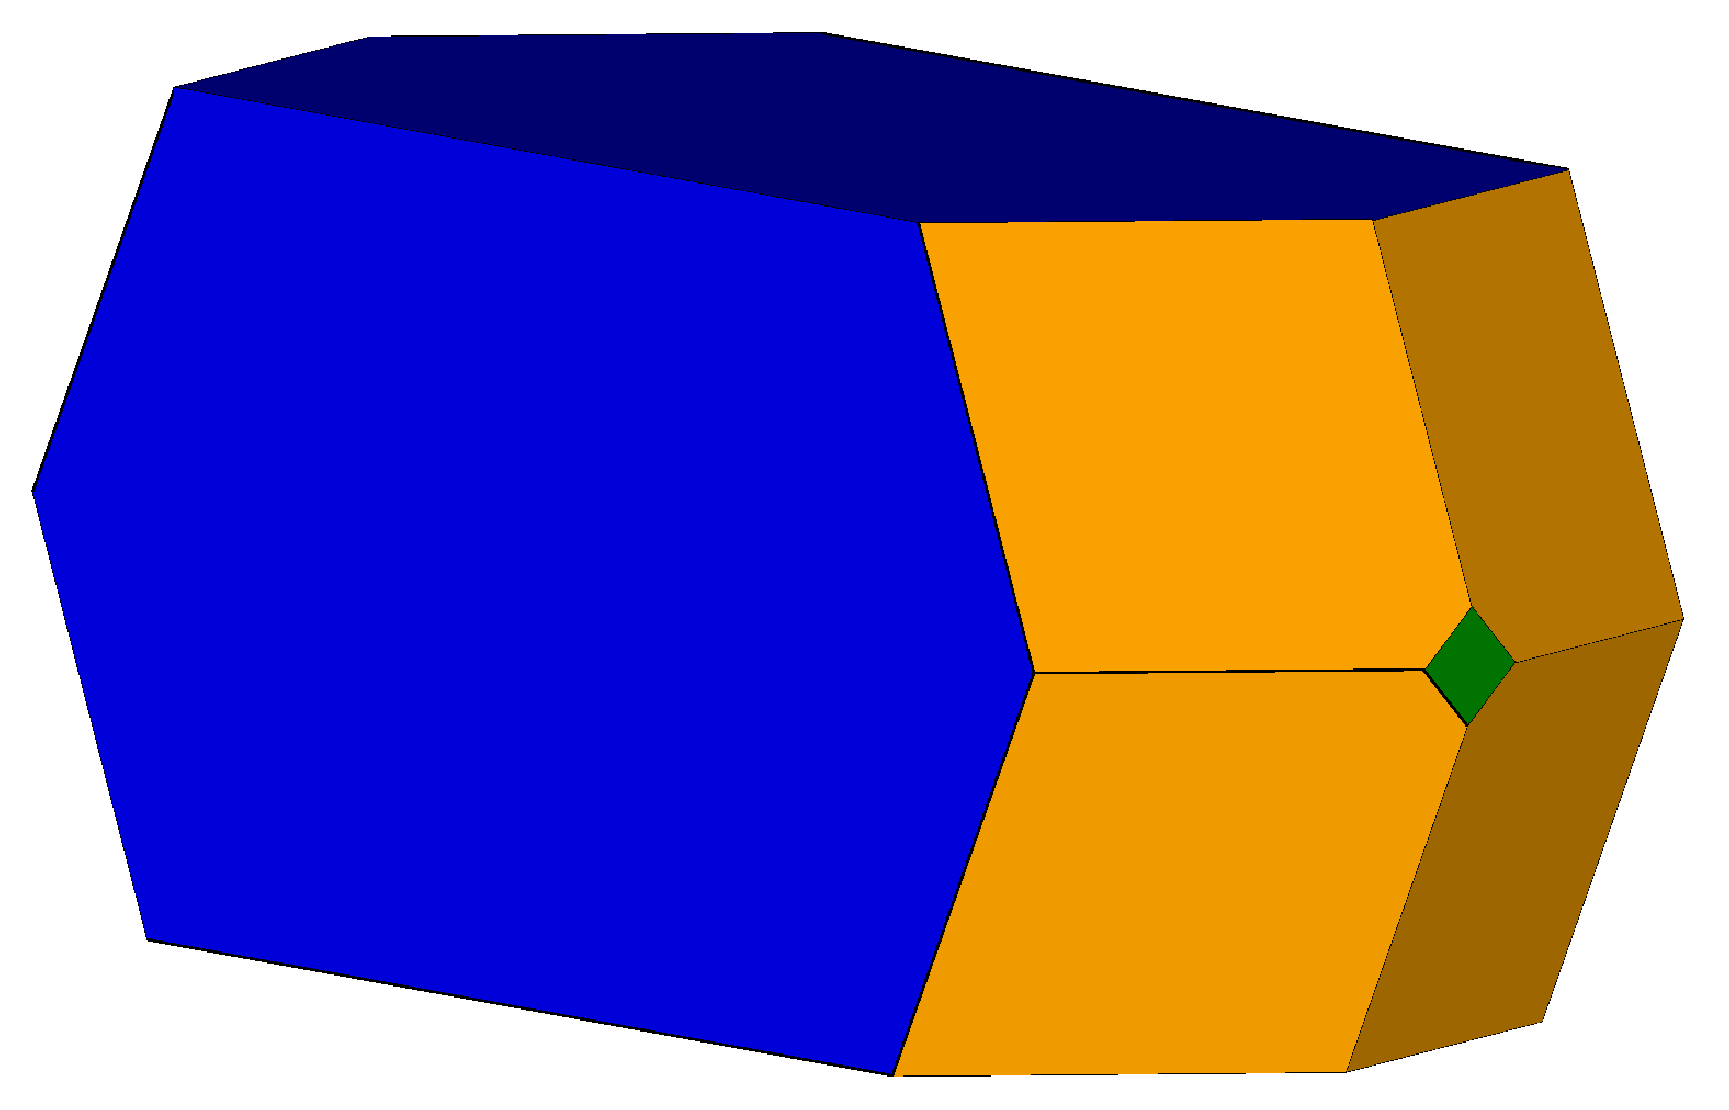
\includegraphics[width=0.4\textwidth]{wulff-pbesol.eps}
	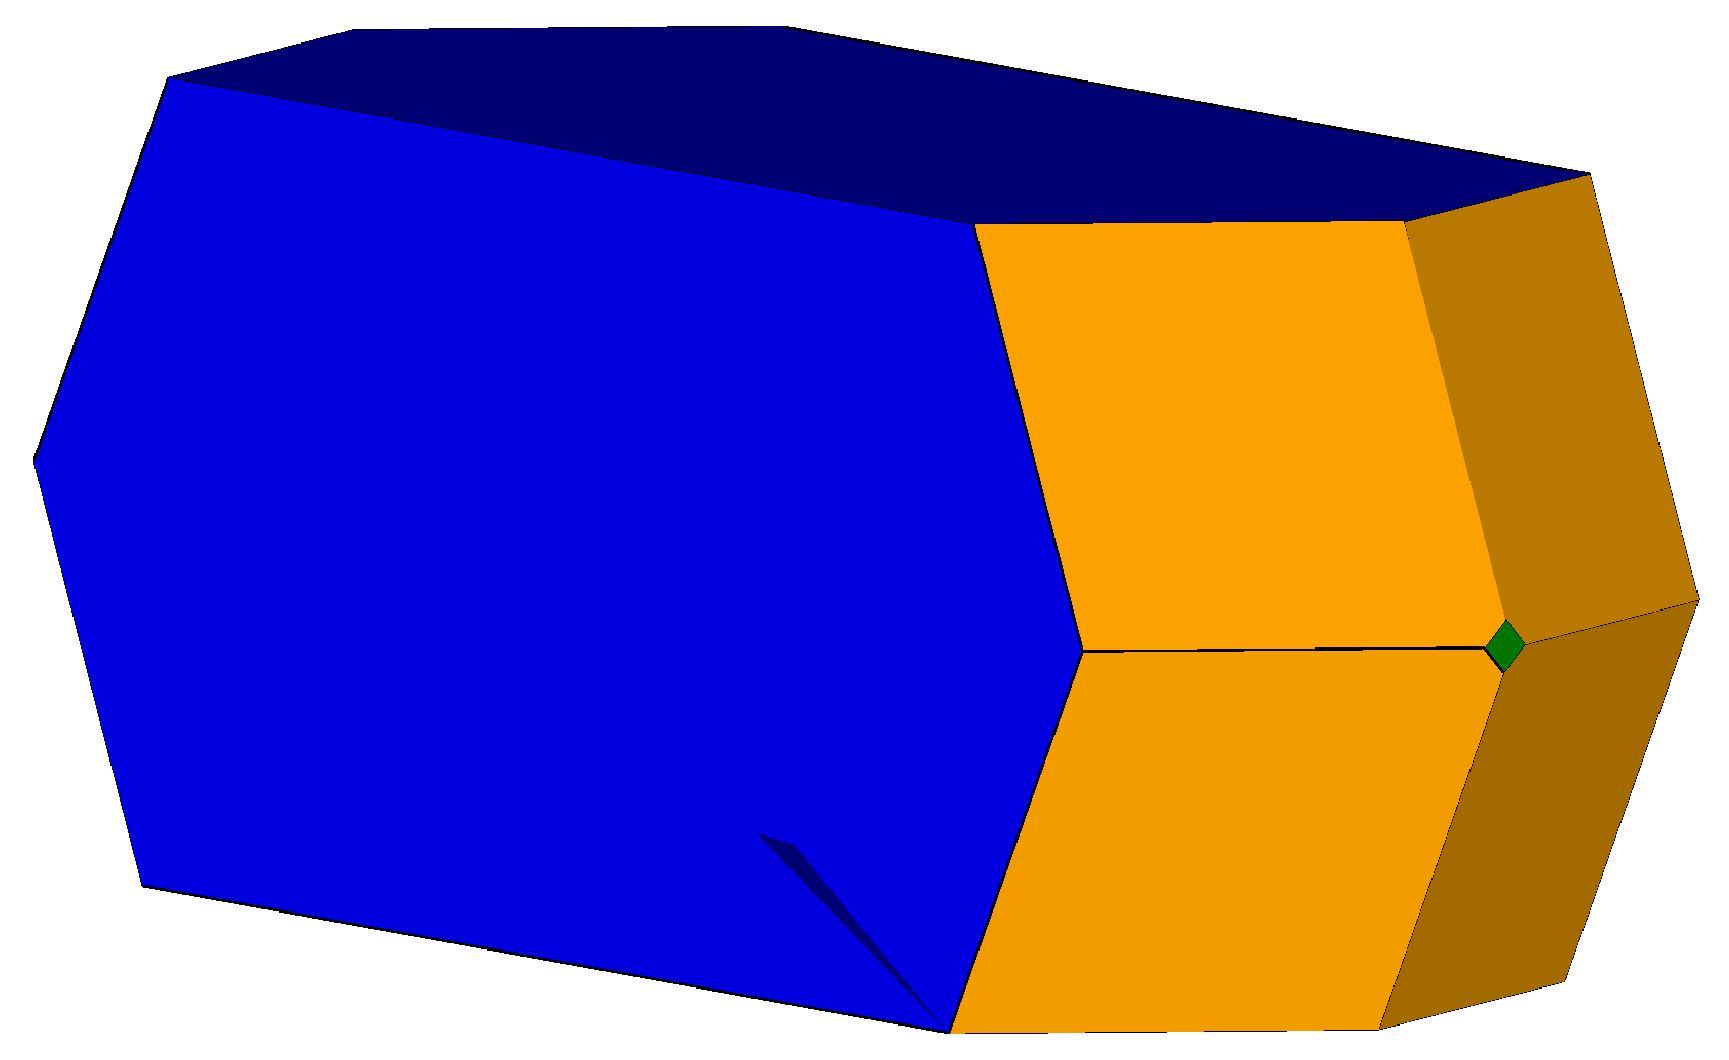
\includegraphics[width=0.4\textwidth]{wulff-pw1pw.eps}
	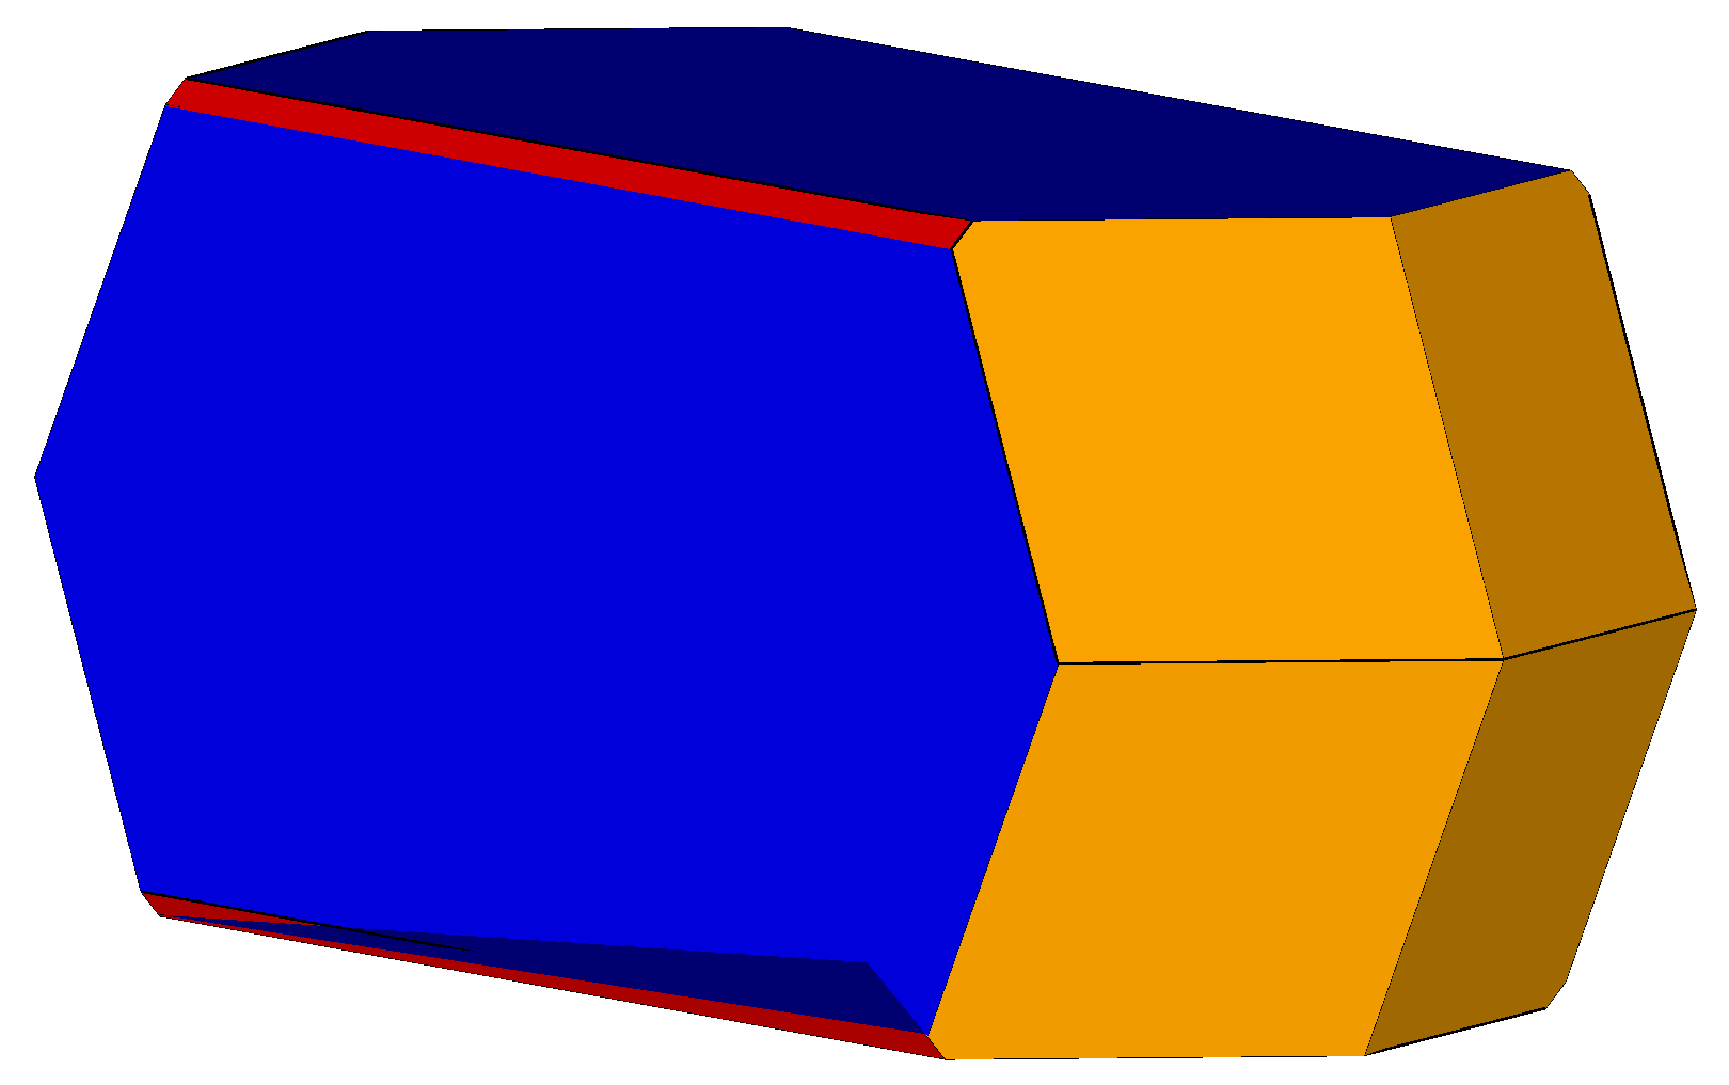
\includegraphics[width=0.4\textwidth]{wulff-theo-lit.eps}
	\includegraphics[width=0.4\textwidth]{rutile_exp.png}
	\caption{Crystal shape of rutile: Wulff construction based on the surface energies calculated with PBESOL (top left), PW1PW (top right), theoretical literature\autocite[]{rutile-surface-energy} (bottom left) and comparison to experimental data\autocite[]{rutile-shape} (bottom right). The surfaces are colored as follows: (110) blue, (101) orange, (001) green, (100) red.}
	\label{fig:wulff}
\end{figure}
%
\newpage
\printbibliography[title={Literature}]
%
\end{document}